% \chapter{Configuration Adaptive AUTOSAR Project and Environment}

% Modern Advanced Driver Assistance Systems (ADAS) increasingly rely on high-performance computing, service-oriented communication, and AI-based perception algorithms to support complex driving scenarios. Functions such as traffic light recognition, object detection, and driver warning systems require not only high computational performance but also flexible software architectures that can evolve over time.

% Traditional automotive software platforms, which are primarily designed for static and tightly coupled embedded systems, are no longer sufficient to meet these requirements. These platforms typically rely on fixed signal-based communication and tightly integrated software stacks, which limit scalability and adaptability. As vehicle systems become more software-intensive and computation-heavy, especially with the integration of artificial intelligence, a more flexible execution and deployment model is required.

% To address these challenges, AUTOSAR introduced the \textit{Adaptive Platform}. Unlike the Classic Platform, the Adaptive Platform supports dynamic deployment, service-oriented architectures, and execution on high performance computing units using POSIX compliant operating systems. This allows automotive applications to adopt modern software engineering practices while still complying with automotive safety and reliability requirements.

% This chapter presents the configuration process of an Adaptive AUTOSAR project and its execution environment. The focus is on how system artefacts, software components, and deployment descriptions are organized and integrated following the Adaptive AUTOSAR Methodology. Compared to classical development flows, the Adaptive approach emphasizes incremental refinement, explicit artefact dependencies, and a clear separation between design, implementation, and deployment phases. This structured methodology is particularly suitable for complex ADAS systems, where multiple software components must interact dynamically at runtime.

% In addition, this chapter describes the configuration and training of the YOLO-MobileNetv4 model used for perception tasks, as well as the cross-compilation of the LiteRT framework for integration into the Adaptive AUTOSAR environment. Finally, a Docker, which based development environment is introduced to ensure reproducibility, portability, and consistency across different development stages.

% The remainder of this chapter is organized as follows. Section~\ref{sec:adaptive_methodology} introduces the Adaptive AUTOSAR methodology and its knowledge base. The configuration and training process of YOLO-MobileNetv4 is discussed afterward. The cross-compilation workflow for the LiteRT framework is then presented, followed by the setup of the Adaptive AUTOSAR Docker environment.

% % TODO: Insert a high-level workflow figure showing Methodology -> AI Model -> Cross Compilation -> Docker Environment

% \section{Adaptive AUTOSAR Methodology}
% \label{sec:adaptive_methodology}
% \subsection{Knowledge Base}

The Adaptive AUTOSAR Methodology is founded on a structured and comprehensive knowledge base that defines how automotive software systems are specified, designed, implemented, and deployed. This knowledge base is standardized by AUTOSAR and documented in the Methodology for Adaptive
Platform (Version R22-11)\cite{AUTOSAR_TR_AdaptiveMethodology_R22-11}. Its purpose is to provide a consistent methodological framework that can be applied across different organizations, toolchains, and system architectures.

The knowledge base defines a set of development phases together with the artefacts that are produced and consumed in each phase. By explicitly modeling artefact relationships, the methodology ensures traceability throughout the system lifecycle, from early architectural descriptions to deployable software units. Such traceability is a key requirement for large-scale automotive software systems, where changes at one abstraction level must be systematically reflected at others.

At the core of the Adaptive AUTOSAR Methodology are the \textit{Method Content Packages}. Each Method Content Package represents a coherent development stage and specifies:
\begin{itemize}
    \item The input artefacts required to initiate the phase,
    \item The output artefacts that are produced or extended,
    \item And the refinement relations between artefacts across phases.
\end{itemize}

This structure supports incremental and iterative development, allowing architectural decisions to be refined step by step while preserving consistency between abstraction levels.

% TODO: Insert figure illustrating Adaptive AUTOSAR Method Content Packages
\begin{figure}[h]
    \centering
    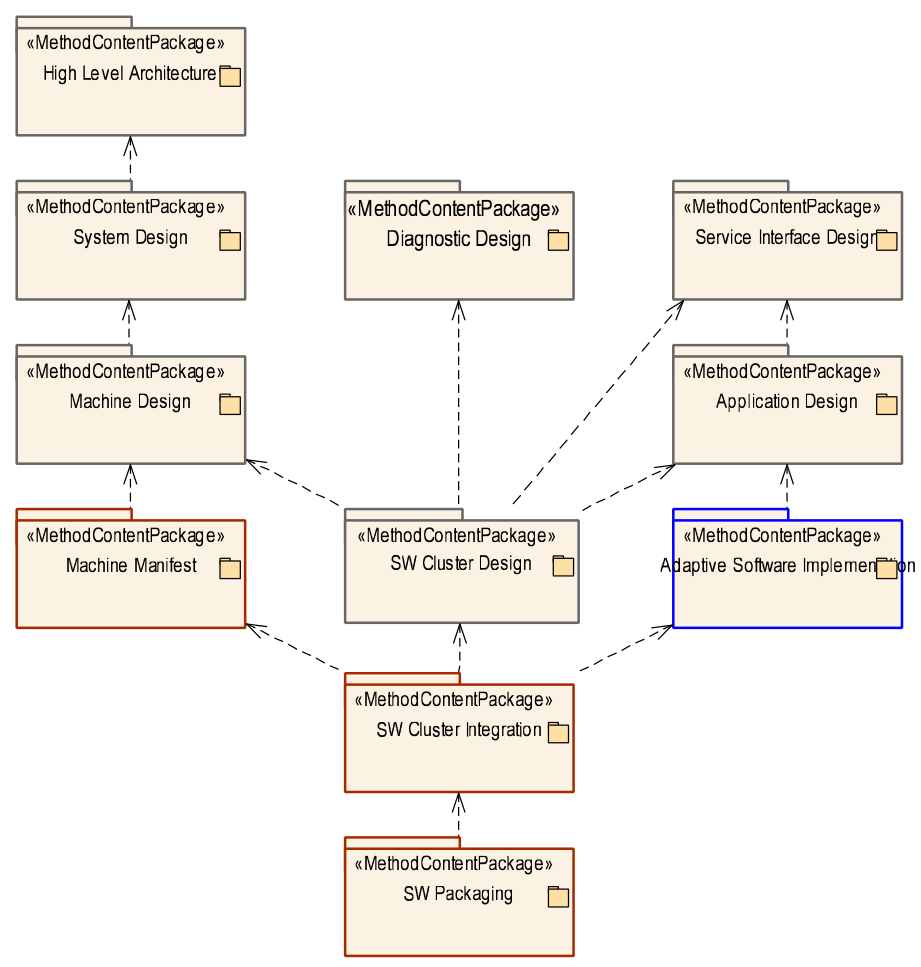
\includegraphics[width=0.75\textwidth]{Images/chap3/image_methodology/knowledgeBase/AdaptiveMethodology.png}
    \vspace{0.5cm}
    \caption{Adaptive Methodology}
    \label{fig:adap_methodology}
\end{figure}

% \subsubsection{High Level Architecture}

% % Figure before explanation
% \begin{figure}[H] % Dùng ht (here, top) là chuẩn nhất
%     \centering
%     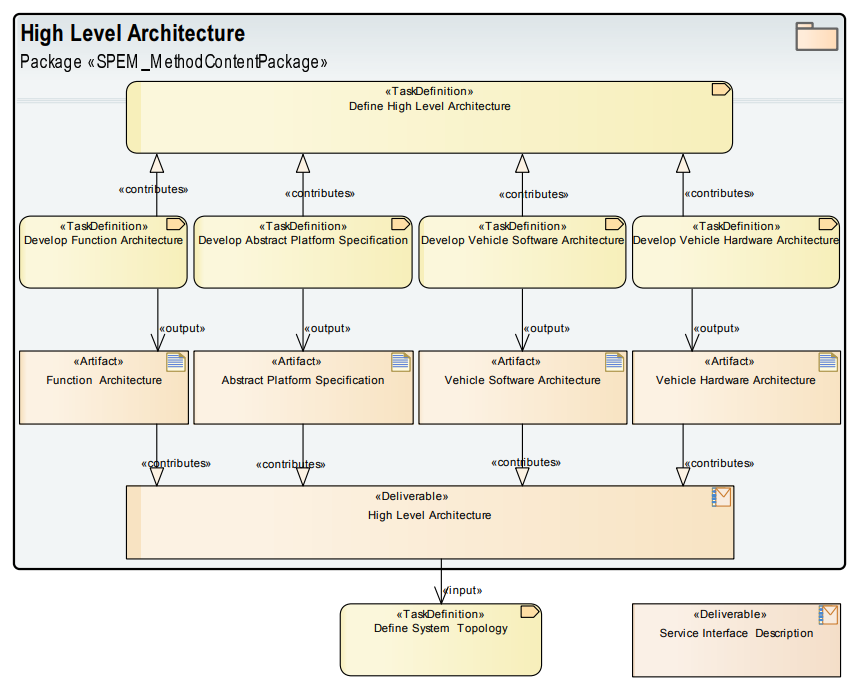
\includegraphics[width=0.75\textwidth]{Images/chap3/image_methodology/knowledgeBase/HLA.png}
%     \vspace{0.5cm}
%     \caption{High Level Architecture in Adaptive AUTOSAR Methodology}
%     \label{fig:hla_architecture} % Đã đổi tên nhãn để không trùng
% \end{figure}

% The High Level Architecture represents the initial and most abstract architectural view within the Adaptive AUTOSAR Methodology. Its primary purpose is to establish a common architectural foundation for the vehicle E/E system before detailed system design and implementation activities are performed.

% As illustrated in Figure~\ref{fig:hla_architecture}, the High Level Architecture is defined through a set of coordinated architectural tasks that collectively contribute to a unified architectural deliverable. These tasks include the development of the Function Architecture, the Abstract Platform Specification, the Vehicle Software Architecture, and the Vehicle Hardware Architecture. Each task addresses a specific architectural concern while remaining independent of concrete implementation decisions.

% The Function Architecture focuses on identifying and structuring the system functions and their logical relationships. It describes what the system is expected to do, without specifying how or where these functions are executed. In parallel, the Abstract Platform Specification defines the abstract execution environment and platform capabilities required by the software, serving as a conceptual bridge between functional requirements and platform realization.

% The Vehicle Software Architecture describes the high level organization of software elements within the vehicle, including major software partitions and their responsibilities. Complementarily, the Vehicle Hardware Architecture captures the high-level hardware structure of the system, including computing units and their relationships, without binding the architecture to specific hardware components.

% The outputs of these architectural tasks are formalized as architectural artefacts. These artefacts collectively contribute to the High-Level Architecture deliverable, which serves as a key input for subsequent methodology phases. In particular, the High Level Architecture provides the architectural context required for defining the system topology and service interface descriptions in later stages.

% By separating functional, software, hardware, and platform concerns at this early stage, the High Level Architecture supports architectural clarity, scalability, and consistency. It ensures that subsequent design and integration activities are grounded in a coherent and well-structured architectural vision.


% \subsubsection{System Design}

% % Figure before explanation
% \begin{figure}[H] % Dùng ht (here, top) là chuẩn nhất
%     \centering
%     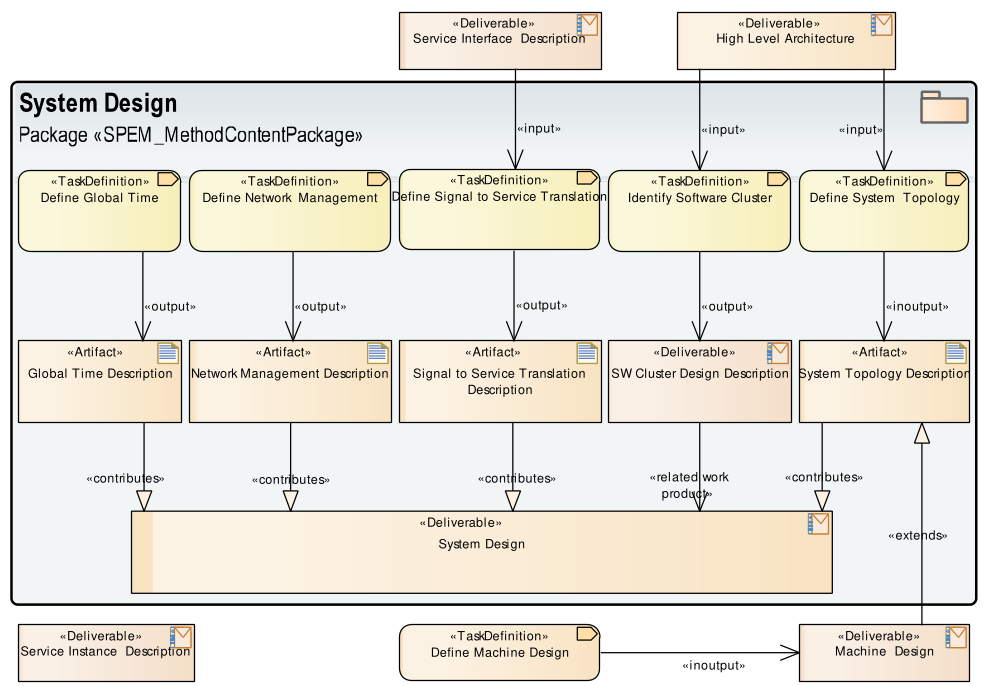
\includegraphics[width=0.75\textwidth]{Images/chap3/image_methodology/knowledgeBase/systemDesign.png}
%     \vspace{0.5cm}
%     \caption{System Design in Adaptive AUTOSAR Methodology}
%     \label{fig:system_design} % Đã đổi tên nhãn để không trùng
% \end{figure}

% The System Design phase refines the architectural concepts established in the High-Level Architecture into a more concrete and structured system-level description. Its primary objective is to define how software elements, communication mechanisms, and system resources are organized and coordinated within the Adaptive AUTOSAR environment.

% As illustrated in the System Design package, this phase consumes key architectural deliverables, including the High Level Architecture and the Service Interface Description, as inputs. Based on these inputs, a set of dedicated design tasks is performed to derive detailed system artefacts that collectively form the System Design deliverable.

% One of the central tasks in this phase is the definition of global timing concepts. The \textit{Define Global Time} task establishes a common time base for the system, which is essential for coordinating distributed software execution and ensuring temporal consistency across different system elements. The resulting Global Time Description contributes to the overall System Design by providing a unified temporal reference.

% In parallel, the \textit{Define Network Management} task specifies how communication networks are controlled and supervised at the system level. This task produces the Network Management Description, which defines network states, transitions, and management strategies. These definitions support reliable communication and controlled system behavior during startup, operation, and shutdown phases.

% Another key task within this phase is the \textit{Define Signal to Service Translation}. This task addresses the mapping between signal-oriented communication and service-oriented communication. The resulting Signal to Service Translation Description enables interaction between system elements that rely on different communication paradigms, ensuring compatibility and interoperability within the Adaptive Platform.

% The System Design phase also includes the identification of software clusters through the \textit{Identify Software Cluster} task. Software clusters group related software elements into coherent deployment units. The resulting Software Cluster Design Description serves as an important intermediate artefact that supports later integration and deployment activities.

% Furthermore, the \textit{Define System Topology} task specifies how system elements are arranged and connected. The System Topology Description captures function groups, network endpoints, and their relationships. This description provides a structural view of the system and serves as a foundation for subsequent deployment and machine-specific design steps.

% All artefacts generated during these tasks contribute to the System Design deliverable. Together, they establish a consistent and detailed system level specification that bridges the gap between high level architectural concepts and later design phases. The System Design deliverable also provides essential inputs for related activities, such as service instance specification and machine design.

% By consolidating timing, communication, clustering, and topology aspects, the System Design phase ensures that the Adaptive AUTOSAR system is coherently structured and ready for further refinement in subsequent methodology stages.


% % TODO: Insert system topology and communication overview figure

% \subsubsection{Service Interface Design}

% % Figure before explanation
% \begin{figure}[H] % Dùng ht (here, top) là chuẩn nhất
%     \centering
%     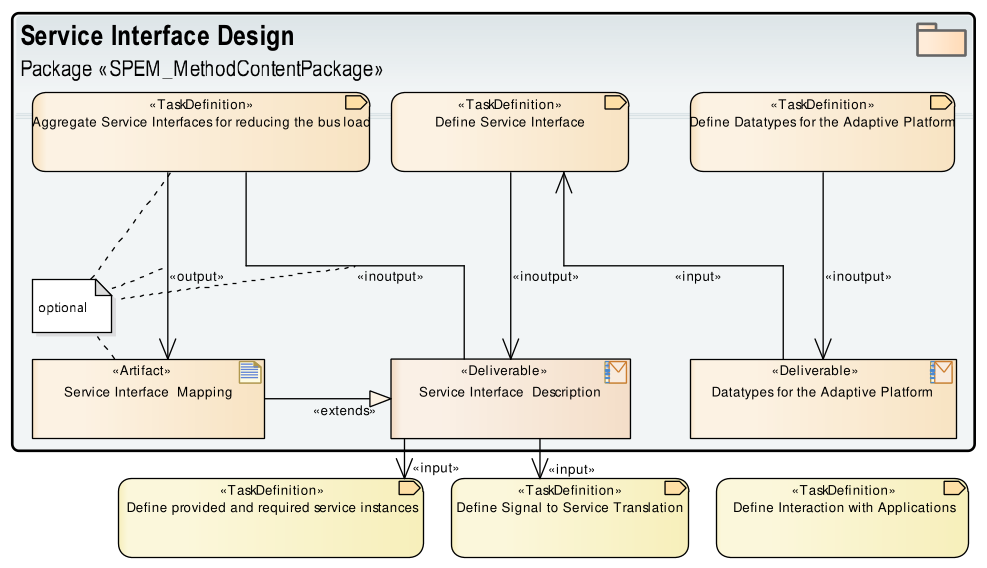
\includegraphics[width=0.75\textwidth]{Images/chap3/image_methodology/knowledgeBase/serviceInterfaceDesign.png}
%     \vspace{0.5cm}
%     \caption{Service Interface Design in Adaptive AUTOSAR Methodology}
%     \label{fig:service_interface_design} % Đã đổi tên nhãn để không trùng
% \end{figure}

% The Service Interface Design defines how Service Interface Descriptions are created, refined, and reused within the Adaptive AUTOSAR development process. This usage scenario explains the sequence of design activities and their associated work products, as illustrated in Figure~\ref{fig:service_interface_design}, focusing on the relationship between service interfaces, datatypes, and interface mappings.

% According to the methodology, Service Interface Descriptions can be obtained through two main usage scenarios: create or change use cases and reuse use cases. These scenarios are not isolated phases but can be integrated into both system design and application design activities, depending on the development context.

% In create or change use cases, Service Interface Descriptions are derived by performing a set of tailored tasks. The central task is the definition of a service interface, which specifies the service operations, events, and communication semantics. In parallel, datatypes for the Adaptive Platform are defined or refined to describe the data exchanged through the service interface. These tasks may be supported by the aggregation of service interfaces, which aims to reduce communication bus load by grouping related service elements when appropriate. The resulting Service Interface Mapping artefact optionally extends the Service Interface Description by documenting how aggregated or related interfaces are organized.

% This scenario is typically applied in a top-down development approach, where architectural or system level considerations drive the definition of service interfaces and datatypes. The outputs of these tasks include the Service Interface Description and the Datatypes for the Adaptive Platform, which together form the primary deliverables of this design stage.

% In reuse use cases, existing Service Interface Descriptions are adopted as inputs with minimal modification. In this case, service interfaces and their associated datatypes are reused from predefined specifications or existing libraries. If required, datatypes may be extended to align with the specific system context. This scenario is commonly applied in a bottom-up development approach and supports efficient reuse across different projects.

% The resulting work products of both scenarios are tailored Service Interface Descriptions and corresponding Datatype Descriptions. These deliverables serve as inputs for subsequent design activities, such as the definition of provided and required service instances, signal-to-service translation, and the specification of interactions with applications.

% By explicitly structuring the creation, aggregation, mapping, and reuse of service interfaces, the Service Interface Design usage scenario ensures consistency, modularity, and reusability of service definitions within the Adaptive AUTOSAR methodology.

% \subsubsection{Application Design}

% % Figure before explanation
% \begin{figure}[H]
%     \centering
%     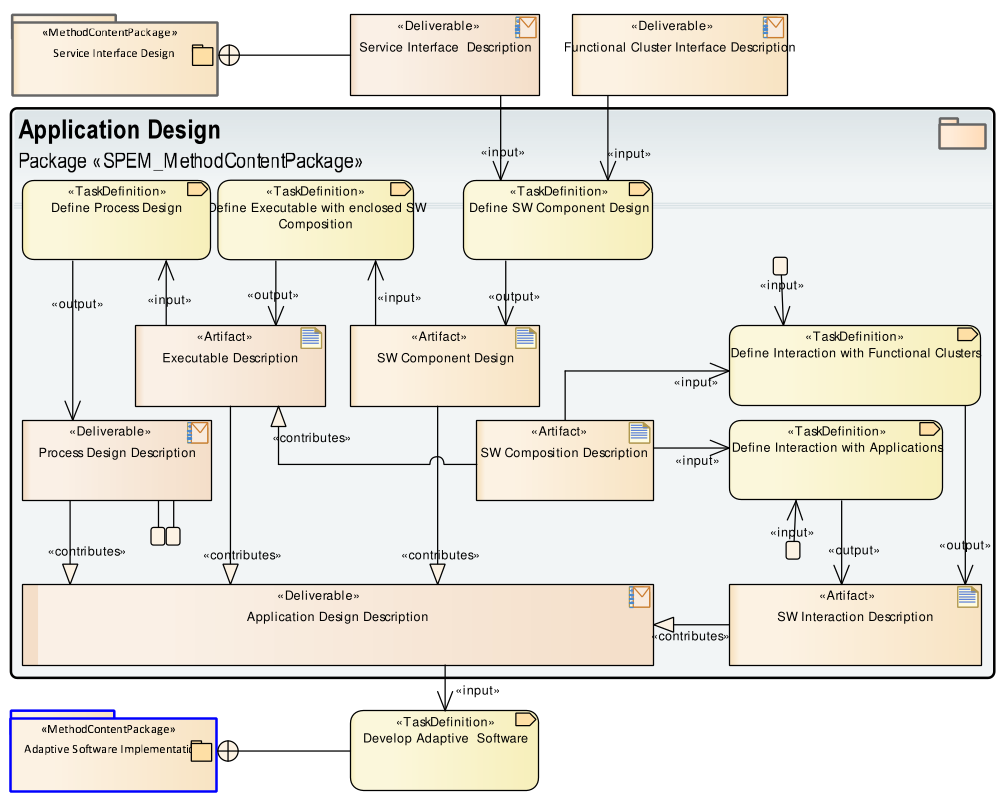
\includegraphics[width=0.75\textwidth]{Images/chap3/image_methodology/knowledgeBase/applicationDesign.png}
%     \vspace{0.5cm}
%     \caption{Application Design in Adaptive AUTOSAR Methodology}
%     \label{fig:application_design}
% \end{figure}

% The Application Design phase refines the outcomes of system level and service-level design into a detailed specification of executable software structures. Its primary objective is to describe how software components are organized, instantiated, and interconnected during runtime execution within the Adaptive AUTOSAR Platform.

% As shown in Figure~\ref{fig:application_design}, this phase takes the Service Interface Description and the Functional Cluster Interface Description as inputs. Based on these artefacts, a set of closely related design activities is carried out, leading to the definition of the overall Application Design Description.

% One of the key activities in this phase is \textit{Define Software (SW) Component Design}. This activity results in the SW Component Design artefact, which specifies the internal structure of software components and their interaction endpoints. These endpoints are expressed through software component (SWC) ports instantiating specific port interfaces at either the application level or the platform level. The SW Component Design establishes the structural basis required for subsequent composition and interaction definitions.

% Another essential activity is \textit{Define Executable with enclosed SW Composition}, which determines how software components are assembled into executable units. Its outcome is the Executable Description, including the SW Composition Description. This description identifies the software components contained within an executable and defines their structural relationships. The execution of this activity requires that all referenced SW Component Designs are already available.

% The runtime realization of executables is addressed by the \textit{Define Process Design} activity. The resulting Process Design Description represents a design time abstraction of the operating system process responsible for instantiating and starting a specific executable. This activity builds upon the Executable Description and provides the link between executable definitions and their runtime execution context.

% Interaction which related aspects are specified through the activities \textit{Define Interaction with Applications} and \textit{Define Interaction with Functional Clusters}. Together, these activities produce the SW Interaction Description, which captures all interaction configurations that are relevant at design time. This includes interactions between application-level software components as well as interactions with platform-level functional clusters. The definition of these interactions depends on the availability of the Process Design Description, the corresponding Executable Description with its SW Composition Description, and the interaction endpoints defined in the SW Component Designs.

% All artefacts produced during the Application Design phase contribute to the Application Design Description deliverable. This deliverable consolidates software component definitions, executable compositions, process abstractions, and interaction configurations into a consistent and comprehensive design representation.

% The activities within the Application Design phase are interdependent and may be performed in an order that best fits the project context. Although the primary focus of this phase is on application-level software, the same design principles and activities may also be applied to platform-level software, particularly when port and port interface concepts are supported.

% The resulting Application Design Description serves as a fundamental input for the subsequent Adaptive Software Implementation phase, where the defined software structures are realized as executable software.

% \subsubsection{Adaptive Software Implementation}

% % Figure before explanation
% \begin{figure}[H]
%     \centering
%     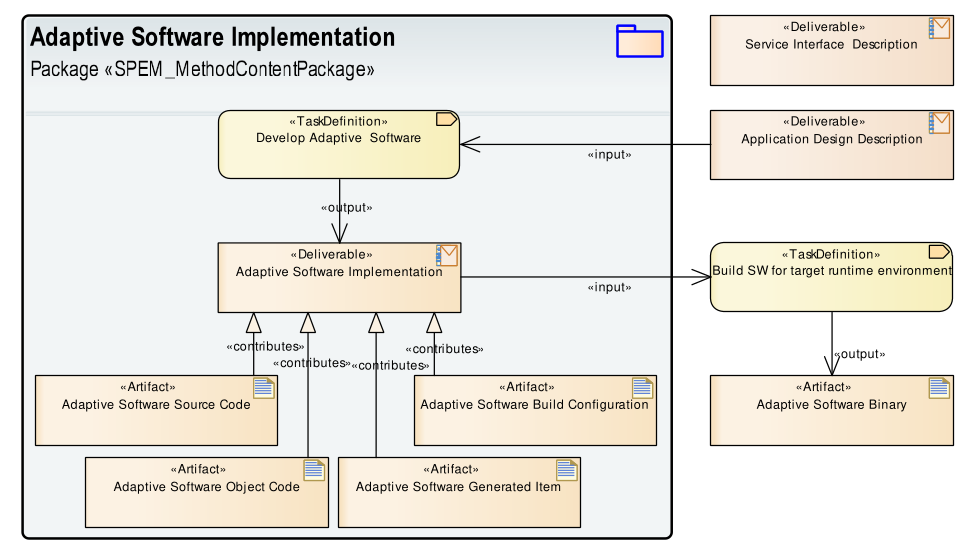
\includegraphics[width=0.75\textwidth]{Images/chap3/image_methodology/knowledgeBase/softwareImplementation.png}
%     \vspace{0.5cm}
%     \caption{Adaptive Software Implementation in Adaptive AUTOSAR Methodology}
%     \label{fig:software_implementation}
% \end{figure}

% The Adaptive Software Implementation phase addresses the realization of software defined during the preceding design stages. Its purpose is to transform the Application Design Description into concrete software artefacts that can be integrated and executed within the Adaptive AUTOSAR runtime environment.

% As depicted in Figure~\ref{fig:software_implementation}, this phase is initiated once the Service Interface Description and the Application Design Description are available. These deliverables provide the necessary interface definitions and structural specifications required to start the implementation activities.

% The central activity of this phase is \textit{Develop Adaptive Software}. This activity encompasses the development of application level and/or platform level Adaptive Software and may include analysis, detailed design, implementation, and testing activities. The development process relies on Adaptive Software Generated Items, such as service proxies and service skeletons, which are derived from service interface definitions and support the implementation of communication ports and port interfaces.

% Depending on the availability of the Adaptive Software Build Configuration, the development process follows different realization paths. When the build configuration is known in advance, software components can be compiled by the developer, and Adaptive Software Object Code can be delivered directly. In contrast, if the build configuration is not available, the developer provides Adaptive Software Source Code, and the compilation is performed later by the integrator.

% The artefacts produced during software development include Adaptive Software Source Code, Adaptive Software Object Code, Adaptive Software Generated Items, and the Adaptive Software Build Configuration. Together, these artefacts contribute to the Adaptive Software Implementation deliverable, which represents the complete implementation result prepared for integration.

% The transformation of the implementation into deployable form is addressed by the activity \textit{Build software (SW) for target runtime environment}. This activity consumes the Adaptive Software Implementation and produces the Adaptive Software Binary. The binary represents the executable form of the software that is suitable for deployment on the target machine and runtime environment.

% Throughout this phase, both application level and platform level Adaptive Software are treated consistently. Each executable requires a main function and an execution manifest, enabling instantiation and deployment within the Adaptive AUTOSAR execution framework.

% The Adaptive Software Implementation deliverable produced in this phase serves as the handover point between software development and integration. It provides the necessary implementation artefacts for subsequent software cluster integration, packaging, and deployment activities.

% \subsubsection{Diagnostic Design}

% % Figure before explanation
% \begin{figure}[H]
%     \centering
%     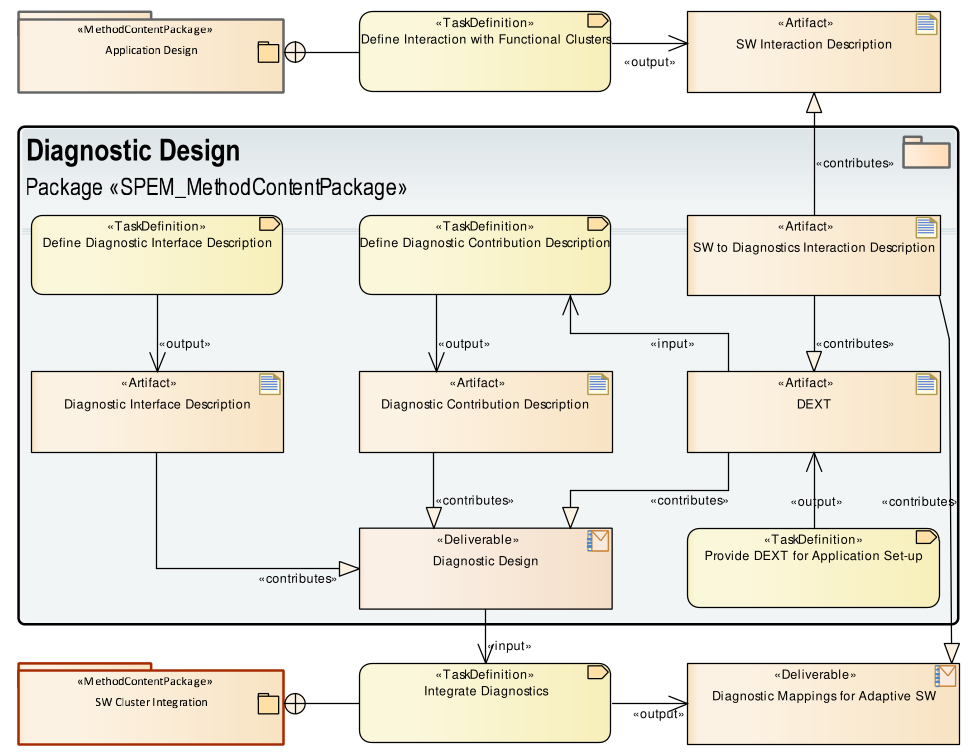
\includegraphics[width=0.75\textwidth]{Images/chap3/image_methodology/knowledgeBase/diagDesign.png}
%     \vspace{0.5cm}
%     \caption{Diagnostic Design in Adaptive AUTOSAR Methodology}
%     \label{fig:diag_design}
% \end{figure}

% The Diagnostic Design phase focuses on defining how diagnostic information is associated with the software structures of the Adaptive AUTOSAR system. Its main objective is to prepare diagnostic which related artefacts that enable consistent monitoring, reporting, and interaction with the diagnostic manager during system operation.

% As shown in Figure~\ref{fig:diag_design}, Diagnostic Design builds on results obtained during the Application Design phase, particularly the SW Interaction Description that captures interactions with functional clusters. These interaction definitions provide the context required to specify diagnostic interfaces and mappings in a systematic manner.

% The activity \textit{Define Diagnostic Interface Description} establishes the diagnostic interfaces that adaptive software components expose for diagnostic purposes. The resulting Diagnostic Interface Description specifies diagnostic port interfaces and their characteristics, allowing diagnostic managers to access diagnostic which relevant data and services in a standardized way.

% Complementing this, the activity \textit{Define Diagnostic Contribution Description} identifies the diagnostic content contributed by software elements within a given context. The Diagnostic Contribution Description determines which parts of the diagnostic configuration are relevant for specific executables or software clusters and are intended to be processed by the diagnostic manager.

% Diagnostic resources and configuration data are collected and structured through the activity \textit{Provide DEXT for Application Setup}. This activity produces or extends the Diagnostic Extract (DEXT), which contains diagnostic resources such as diagnostic data identifiers, diagnostic events, enable conditions, and operation cycles. The DEXT acts as a reusable container for diagnostic configuration and may cover multiple executables, diagnostic managers, and software clusters across the vehicle.

% The association between diagnostic resources and software interaction endpoints is captured in the SW to Diagnostics Interaction Description. This artefact specifies how diagnostic information is mapped to software component ports at design time and contributes both to the Diagnostic Design deliverable and to the DEXT. It represents an intermediate form of diagnostic mappings that is refined during later integration steps.

% All artefacts produced during this phase, including the Diagnostic Interface Description, Diagnostic Contribution Description, SW to Diagnostics Interaction Description, and the DEXT, collectively contribute to the Diagnostic Design deliverable. This deliverable provides a consolidated view of the diagnostic configuration that is prepared for further integration activities.

% The Diagnostic Design deliverable is subsequently used as input for the \textit{Integrate Diagnostics} activity during Software Cluster Integration. In that phase, diagnostic mappings are finalized by associating diagnostic resources with concrete executable instances and operating system processes, resulting in the Diagnostic Mappings for Adaptive Software.

% By structuring diagnostic interface definition, contribution specification, and resource extraction as distinct but related activities, the Diagnostic Design phase supports a clear and maintainable diagnostic configuration process within the Adaptive AUTOSAR methodology.

% \subsubsection{Machine Design}

% % Figure before explanation
% \begin{figure}[H]
%     \centering
%     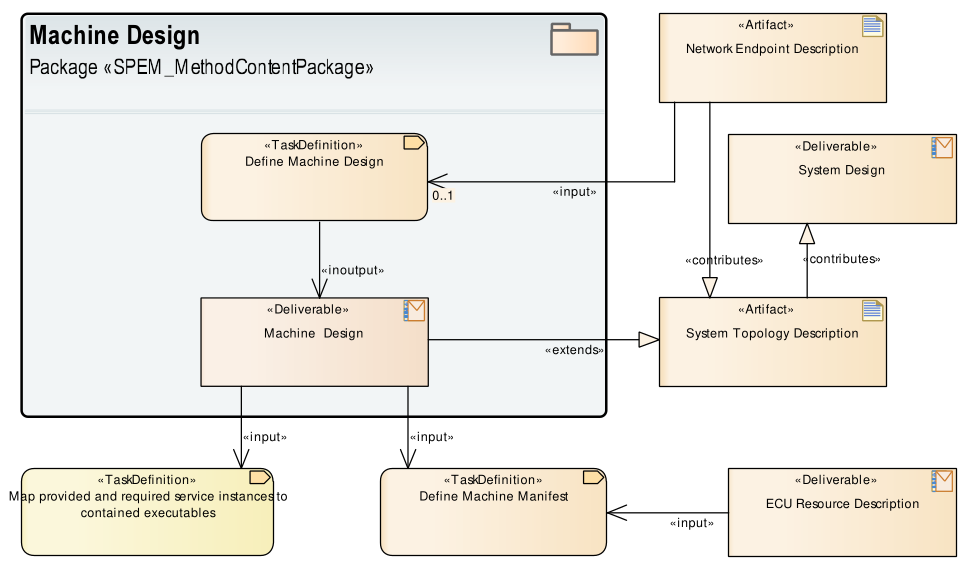
\includegraphics[width=0.75\textwidth]{Images/chap3/image_methodology/knowledgeBase/machineDesign.png}
%     \vspace{0.5cm}
%     \caption{Machine Design in Adaptive AUTOSAR Methodology}
%     \label{fig:machine_design}
% \end{figure}

% The Machine Design phase addresses the specification of a machine from a communication and deployment standpoint within the Adaptive AUTOSAR Platform. Its aim is to describe the characteristics of a machine that are required for software execution and service communication, taking into account system level topology information and the capabilities of the target ECU.

% Figure~\ref{fig:machine_design} provides an overview of the activities involved in this phase. The core activity, \textit{Define Machine Design}, derives a machine-oriented configuration by using network endpoint information defined during System Design. In particular, the System Topology Description and the associated Network Endpoint Description supply the addressing and service discovery parameters needed to shape the communication behavior of the machine.

% The result of this activity is captured in the Machine Design deliverable. This deliverable augments the existing System Topology Description by introducing machine specific communication constraints and requirements. At this stage, the design remains independent of a concrete hardware realization and represents a prospective configuration for a machine.

% Beyond defining communication aspects, the Machine Design also provides the basis for associating software deployment elements with the machine. Through the activity \textit{Map provided and required service instances to contained executables}, service instances are linked to executables that are intended to run on the machine. This association clarifies how services are realized by software units within the machine context.

% The adaptation of the machine configuration to a specific hardware platform is performed in a subsequent activity, \textit{Define Machine Manifest}. This activity combines the Machine Design with the ECU Resource Description, which details the resources and limitations of the target ECU. The outcome is the Machine Manifest, representing a machine configuration that is fully aligned with the characteristics of a real ECU.

% From a methodological viewpoint, machine configuration follows a two-step process. The first step establishes the communication structure of a machine and yields the Machine Design. This step may be carried out in a top-down manner, guided by an existing System Design, or in a bottom-up manner, where machine-specific communication definitions are created locally and may later contribute to the overall system topology.

% The second step focuses on hardware-specific realization and results in the Machine Manifest. This separation between prospective machine definition and ECU specific configuration supports a clear allocation of responsibilities between system designers and integrators, while maintaining flexibility during system integration.

% \subsubsection{Machine Manifest}

% % Figure before explanation
% \begin{figure}[H]
%     \centering
%     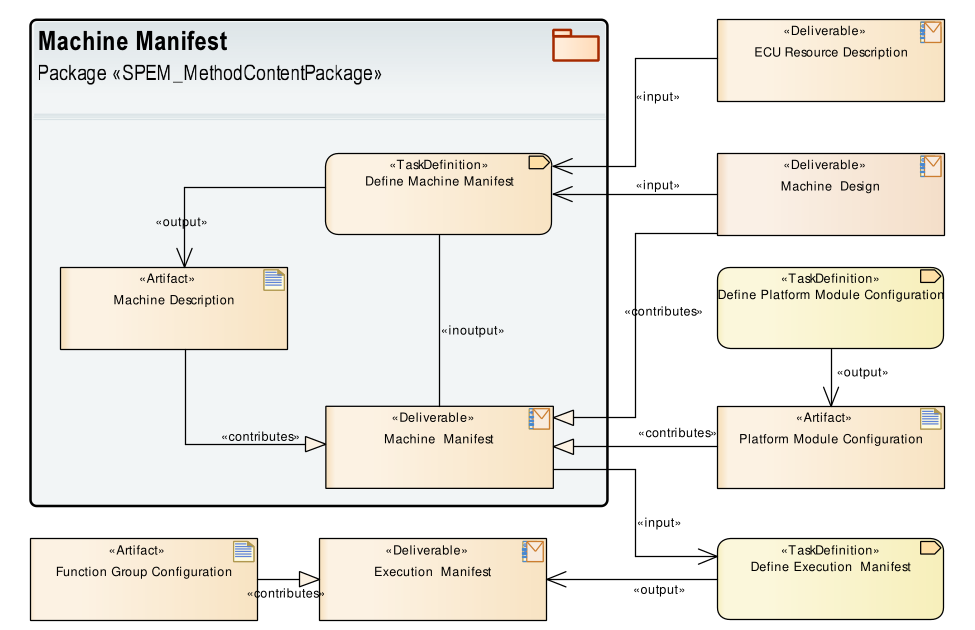
\includegraphics[width=0.75\textwidth]{Images/chap3/image_methodology/knowledgeBase/machineManifest.png}
%     \vspace{0.5cm}
%     \caption{Machine Manifest in Adaptive AUTOSAR Methodology}
%     \label{fig:machine_manifest}
% \end{figure}

% The Machine Manifest phase specifies the final configuration of a machine that is ready to be deployed on a concrete ECU within the Adaptive AUTOSAR Platform. Its purpose is to consolidate communication-related design results with hardware resource information and platform-specific configurations into a single, deployment ready description.

% Figure~\ref{fig:machine_manifest} outlines the activities and work products involved in this phase. The primary activity, \textit{Define Machine Manifest}, is initiated once the Machine Design and the ECU Resource Description are available. While the Machine Design provides a prospective view of the machine configuration, the ECU Resource Description defines the concrete hardware resources offered by the target ECU.

% The outcome of this activity is the Machine Manifest deliverable. The Machine Manifest integrates several key elements. First, it contains the Machine Description, which describes the available hardware resources of the ECU, such as processing units, memory resources, sensors, actuators, and other relevant hardware elements. This information is derived from the ECU Resource Description and tailored to the specific machine instance.

% Second, the Machine Manifest incorporates the Machine Design, thereby preserving the communication structure and network-related configuration that was defined during the Machine Design phase. This ensures that the communication requirements identified earlier are consistently realized on the target ECU.

% In addition, platform-specific aspects are addressed through the activity \textit{Define Platform Module Configuration}. This activity produces Platform Module Configuration artefacts, which specify the machine-specific configuration of Adaptive Platform modules. These configurations may include the operating system setup, platform services such as network management and diagnostics, as well as foundation modules like logging and tracing. The resulting Platform Module Configurations contribute directly to the Machine Manifest.

% The configuration of software execution is captured by the activity \textit{Define Execution Manifest}. This activity produces the Execution Manifest, which specifies which executables are instantiated on the machine and how they are mapped to processes. The Execution Manifest may also include Function Group Configurations that control the activation and deactivation of software elements. The Execution Manifest contributes to the Machine Manifest by defining the runtime behavior of software on the machine.

% From a process perspective, the Machine Manifest is typically assembled in an incremental manner. Communication-related configurations originating from the Machine Design are collected first, followed by the integration of hardware resource descriptions and platform module configurations. As additional configuration information becomes available, the Machine Manifest may be iteratively extended and refined.

% By consolidating machine-specific communication settings, hardware resource descriptions, platform module configurations, and execution information, the Machine Manifest provides a complete and consistent representation of a machine that is ready for deployment within the Adaptive AUTOSAR ecosystem.

% \subsubsection{Software Cluster Design, Integration, and Packaging}

% The phases of Software Cluster Design, Software Cluster Integration, and Software Packaging together form the final preparation steps that transform implemented Adaptive AUTOSAR software into deployable units. These phases consolidate design results, integrate software components with their configurations, and prepare complete software packages for deployment on target machines.

% Software Cluster Design focuses on defining logical groupings of software elements that belong together from a deployment and lifecycle perspective. A software cluster typically bundles application level software, required platform services, and related configuration artifacts into a coherent unit. The purpose of this phase is not to define execution details, but to establish clear cluster boundaries, dependencies, and responsibilities that simplify later integration and deployment activities.

% Based on the cluster definitions, Software Cluster Integration performs the concrete assembly of software and configuration artifacts. During this phase, Adaptive Software Implementations, design descriptions, machine which related information, and diagnostic configurations are brought together and checked for consistency. Integration activities refine execution which related information, such as the association of executables with machines and processes, and complete interaction and diagnostic mappings that could only be finalized once all involved elements are known. As a result, the integrated software cluster represents a consistent and executable view of the system for a specific deployment context.

% Software Packaging completes the workflow by preparing integrated software clusters for delivery and deployment. In this phase, all relevant artifacts, such as software binaries, manifests, configuration files and generated items which are collected and organized into software packages. These packages are structured in a way that supports deployment, update, and lifecycle management, while preserving a clear separation between different software clusters.

% By combining cluster definition, integration, and packaging into a structured workflow, these phases provide a clear transition from implemented software to deployable units. This approach supports modularity, reuse, and scalable integration, which are essential characteristics of the Adaptive AUTOSAR methodology.

% \subsubsection{Summary}

% This section has presented an overview of the Adaptive AUTOSAR knowledge base and its role in structuring the development of complex automotive software systems. The methodology defines a clear sequence of development phases, each supported by well-defined artefacts and responsibilities.

Starting from high-level architectural descriptions, the methodology guides the refinement of system structure, service interfaces, application design, and software implementation. Subsequent phases address diagnostics, machine-specific configuration, and the preparation of software for deployment. Each phase builds upon the results of previous stages, ensuring consistency and traceability throughout the development process.

By explicitly modeling artefact dependencies and separating design, implementation, integration, and deployment concerns, the Adaptive AUTOSAR Methodology supports systematic system development. This approach improves scalability, facilitates reuse, and simplifies integration in large and evolving software systems.

The following section explains how the most important Method Content Packages are configured in this project and how they are refined into concrete Adaptive AUTOSAR artefacts.

% Overall, the knowledge base provides a solid methodological foundation for configuring and deploying Adaptive AUTOSAR systems. It enables a structured transition from abstract system concepts to deployable software units while maintaining clarity and consistency across the entire system lifecycle.


\subsection{Project Methodology}

In this project, the Adaptive AUTOSAR system is developed using the \texttt{Autosar.io} tool provided by PopcornSAR. Autosar.io is a configuration-oriented modeling environment that allows users to systematically define and organize an Adaptive AUTOSAR project through a set of well-structured design sections. Instead of focusing on source code implementation, the tool guides users to configure machines, services, and applications by following the standard Adaptive AUTOSAR modeling workflow.

\begin{figure}[H]
    \centering
    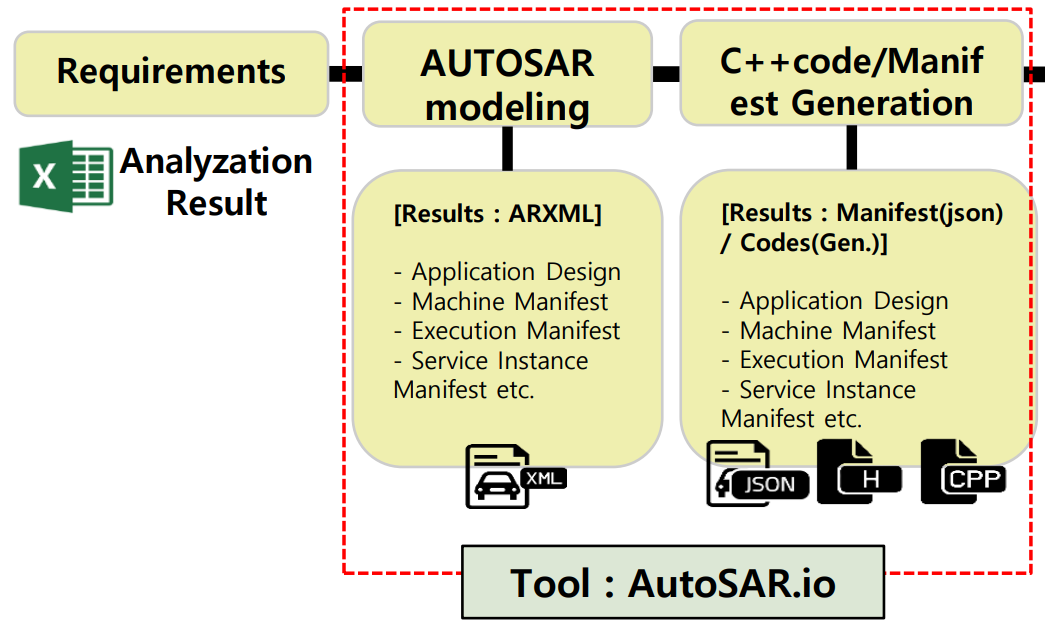
\includegraphics[width=0.75\textwidth]{Images/toolchains/autosario.png}
    \vspace{0.5cm}
    \caption{Autosar.io tool supporting configuration workflow for Adaptive AUTOSAR systems}
    \label{fig:autosario}
\end{figure}

Autosar.io provides dedicated design views that correspond directly to the configuration steps presented in this section, including Machine Design and Machine Manifest creation, Service Interface Design and Mapping, and Adaptive Application Design. Through these views, users can specify network endpoints, service discovery parameters, service interfaces, service instances, application executables, processes, startup behavior, and process-to-machine mappings. Each configuration step produces AUTOSAR-compliant artifacts such as ARXML descriptions and manifests, ensuring consistency between design intent and deployment configuration.

By using Autosar.io, users can incrementally build the system configuration in a top-down manner, where abstract architectural decisions are progressively refined into concrete runtime configurations. This approach enables clear separation between machine-level configuration, service-level communication design, and application-level deployment. As demonstrated throughout this section, Autosar.io acts as the central tool that connects all configuration stages, allowing users to define a complete Adaptive AUTOSAR system in a structured, traceable, and standardized way before moving to implementation and integration phases.

%introduce Autosar.io tool, this is a tool help configuring project based on Adaptive AUTOSAR
\subsubsection{High Level Architecture}
\begin{figure}[H]
    \centering
    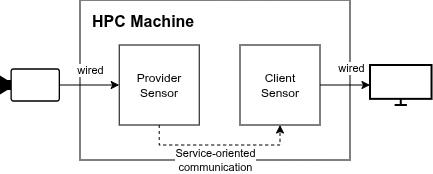
\includegraphics[width=0.75\textwidth]{Images/chap3/image_methodology/machineDesign/high_level.png}
    \vspace{0.5cm}
    \caption{High Level Architecture of Prototype Project}
    \label{fig:hla_project}
\end{figure}

Based on the defined high-level architecture, the Adaptive AUTOSAR configuration process is carried out in a stepwise manner, following the recommended methodology. The overall system design is progressively refined from an abstract architectural view to concrete deployment and execution artifacts.

First, the Machine Design and Machine Manifest are configured to define the physical execution environment of the system. This step specifies the target machine, network interfaces, service discovery settings, operating system platform modules, and lifecycle-related parameters, forming the foundation on which all applications and services are deployed.

Next, the Service Interface Design and Mapping phase focuses on defining the service-oriented communication between applications. During this stage, data types, service interfaces, service instances, and deployment configurations are specified, and abstract service definitions are bound to concrete network endpoints. This step enables standardized and loosely coupled interaction between the Provider Sensor and Client Sensor.

Finally, the Application Design phase models the adaptive applications themselves. Executables are defined and configured, ports are mapped to service interfaces, application processes are created, and startup and lifecycle behaviors are specified. Through this step, the logical application design is concretely mapped onto the target machine, completing the system configuration prior to code and manifest generation.

\subsubsection{Machine Design and Machine Manifest}

% Define Ethernet network endpoint
\begin{figure}[H]
    \centering
    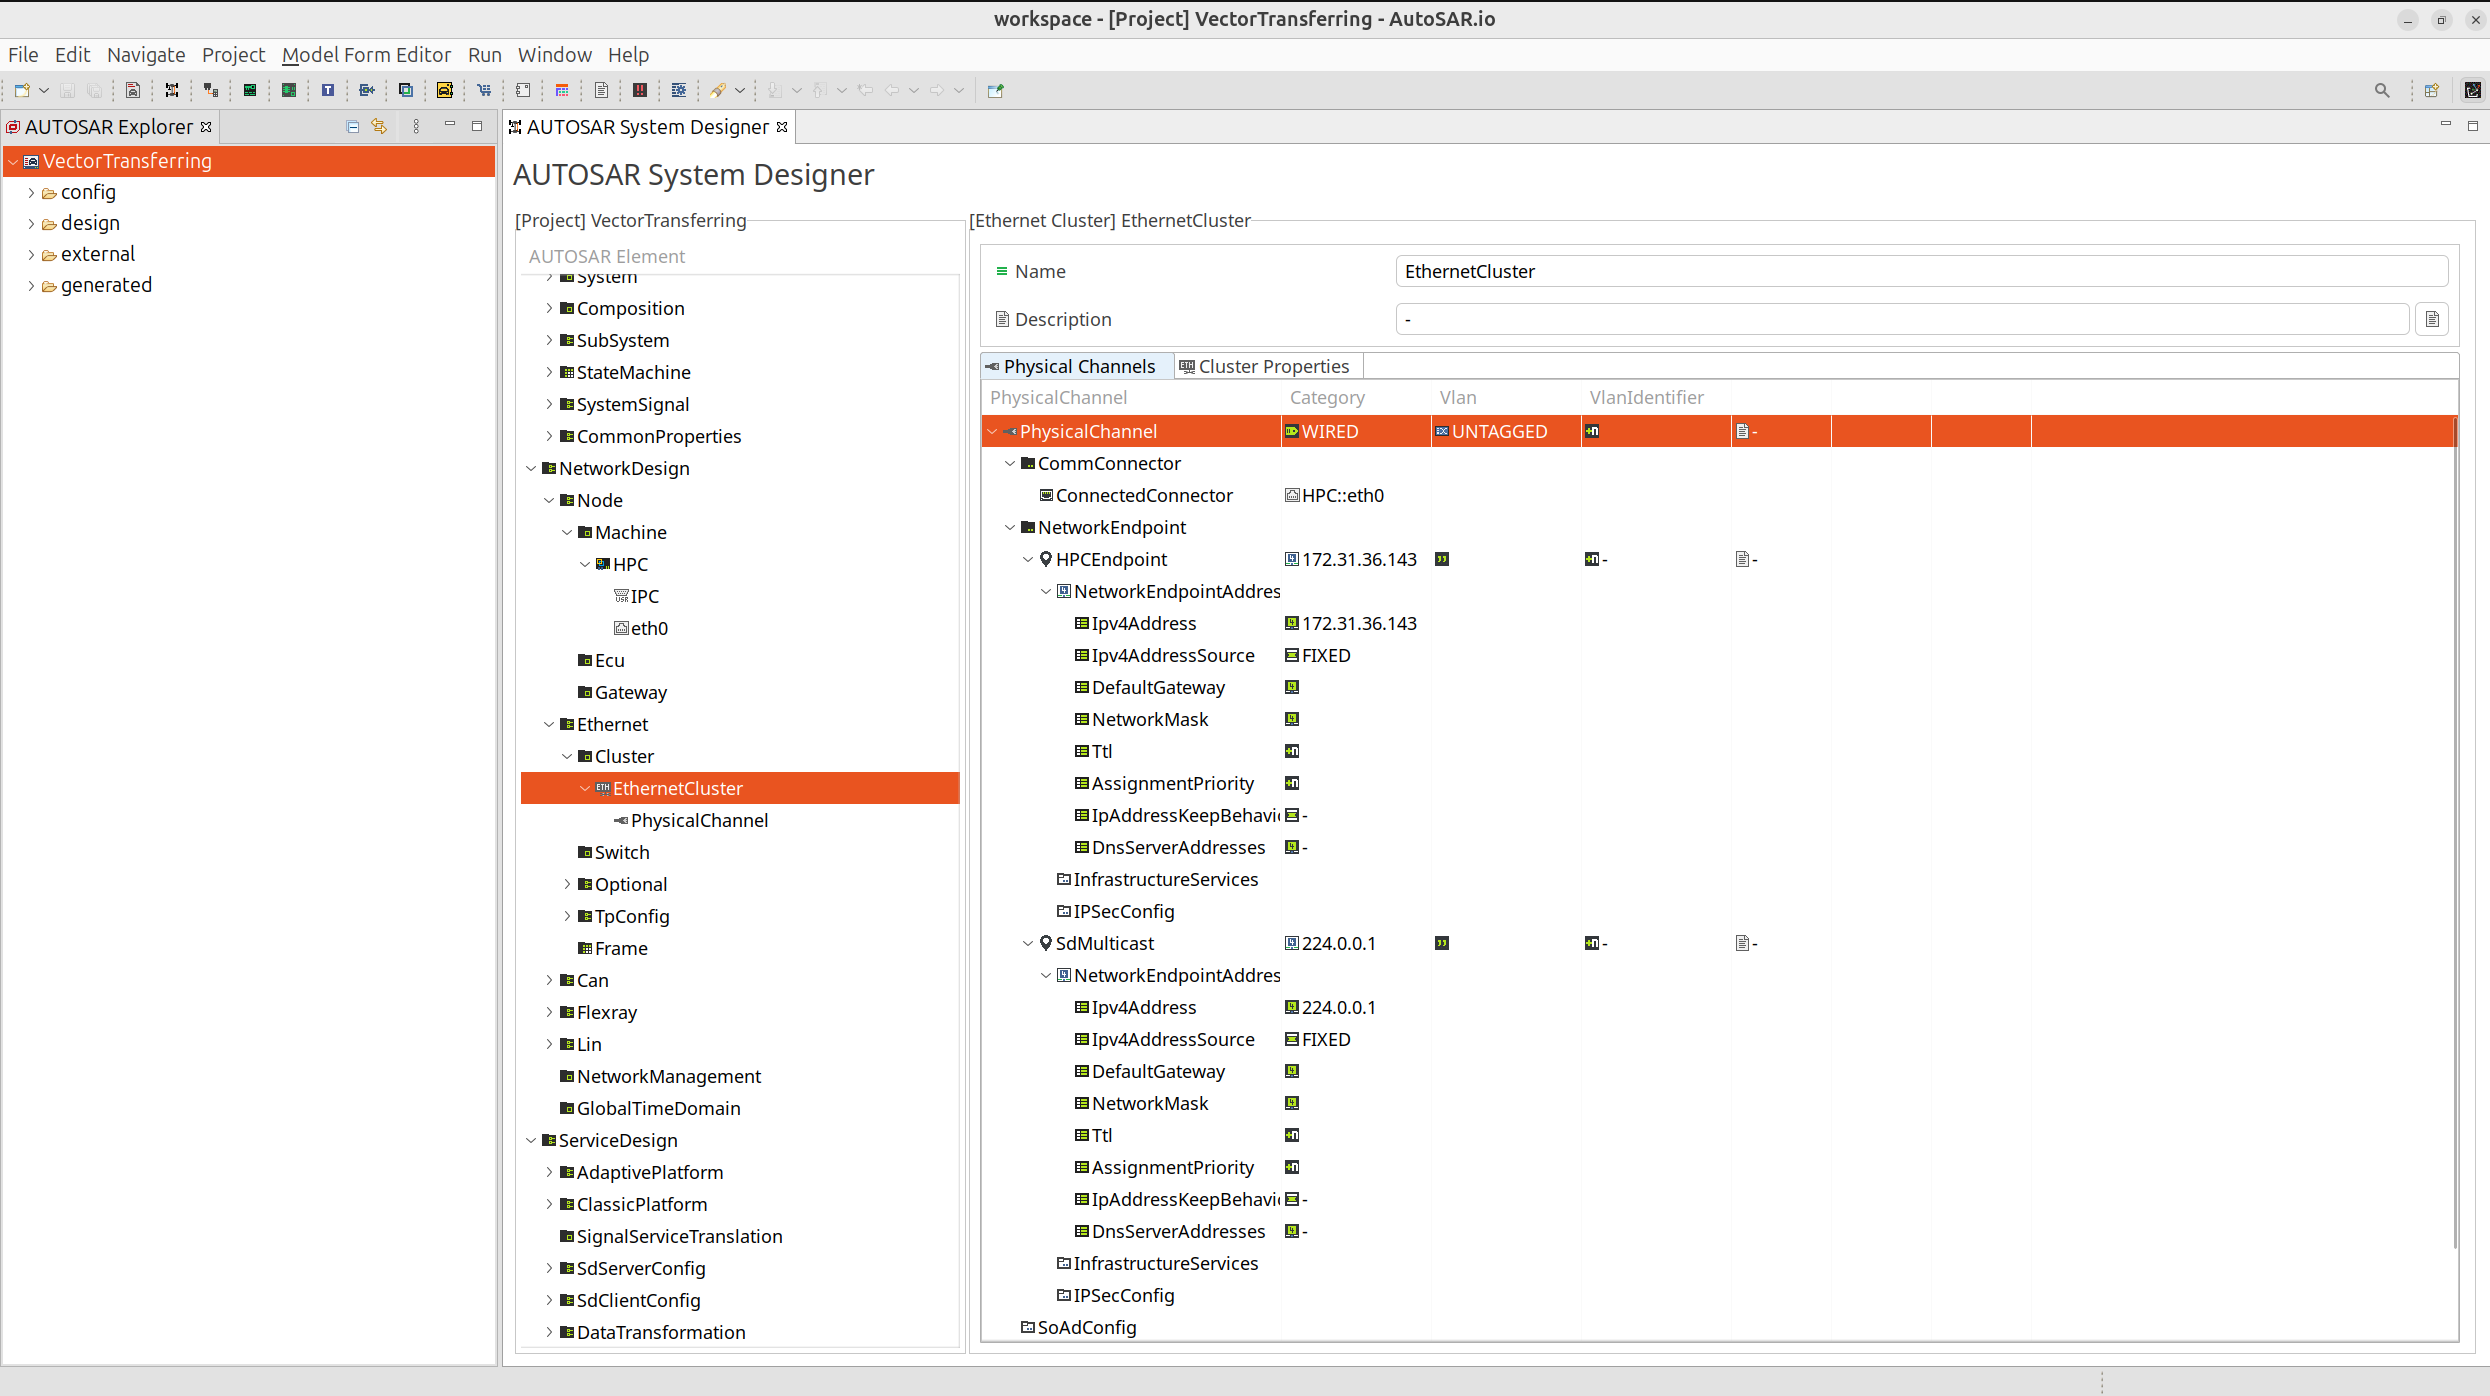
\includegraphics[width=0.75\textwidth]{Images/chap3/image_methodology/machineDesign/defineEthernet.png}
    \vspace{0.5cm}
    \caption{Definition of Ethernet Network Endpoint in Machine Design}
    \label{fig:machine_define_ethernet}
\end{figure}

Figure~\ref{fig:machine_define_ethernet} illustrates the detailed configuration of an Ethernet network endpoint within the AUTOSAR System Designer. An EthernetCluster is defined with a wired physical channel, where the VLAN mode is set to untagged, indicating that no VLAN identifier is applied to the network traffic. The machine node labeled HPC is connected to this cluster through the communication connector HPC eth0, which represents the physical Ethernet interface of the target machine.

The network endpoint configuration specifies a fixed IPv4 address of 172.31.36.143, with the address source explicitly defined as fixed to ensure deterministic network behavior. In addition to the unicast endpoint, a multicast configuration is also present using the IPv4 address 224.0.0.1, which is commonly used for service discovery communication. These settings collectively define how the machine participates in both point to point and multicast Ethernet communication, forming a stable networking foundation for Adaptive AUTOSAR service based applications.

% Add Ethernet configuration to Machine Design
\begin{figure}[H]
    \centering
    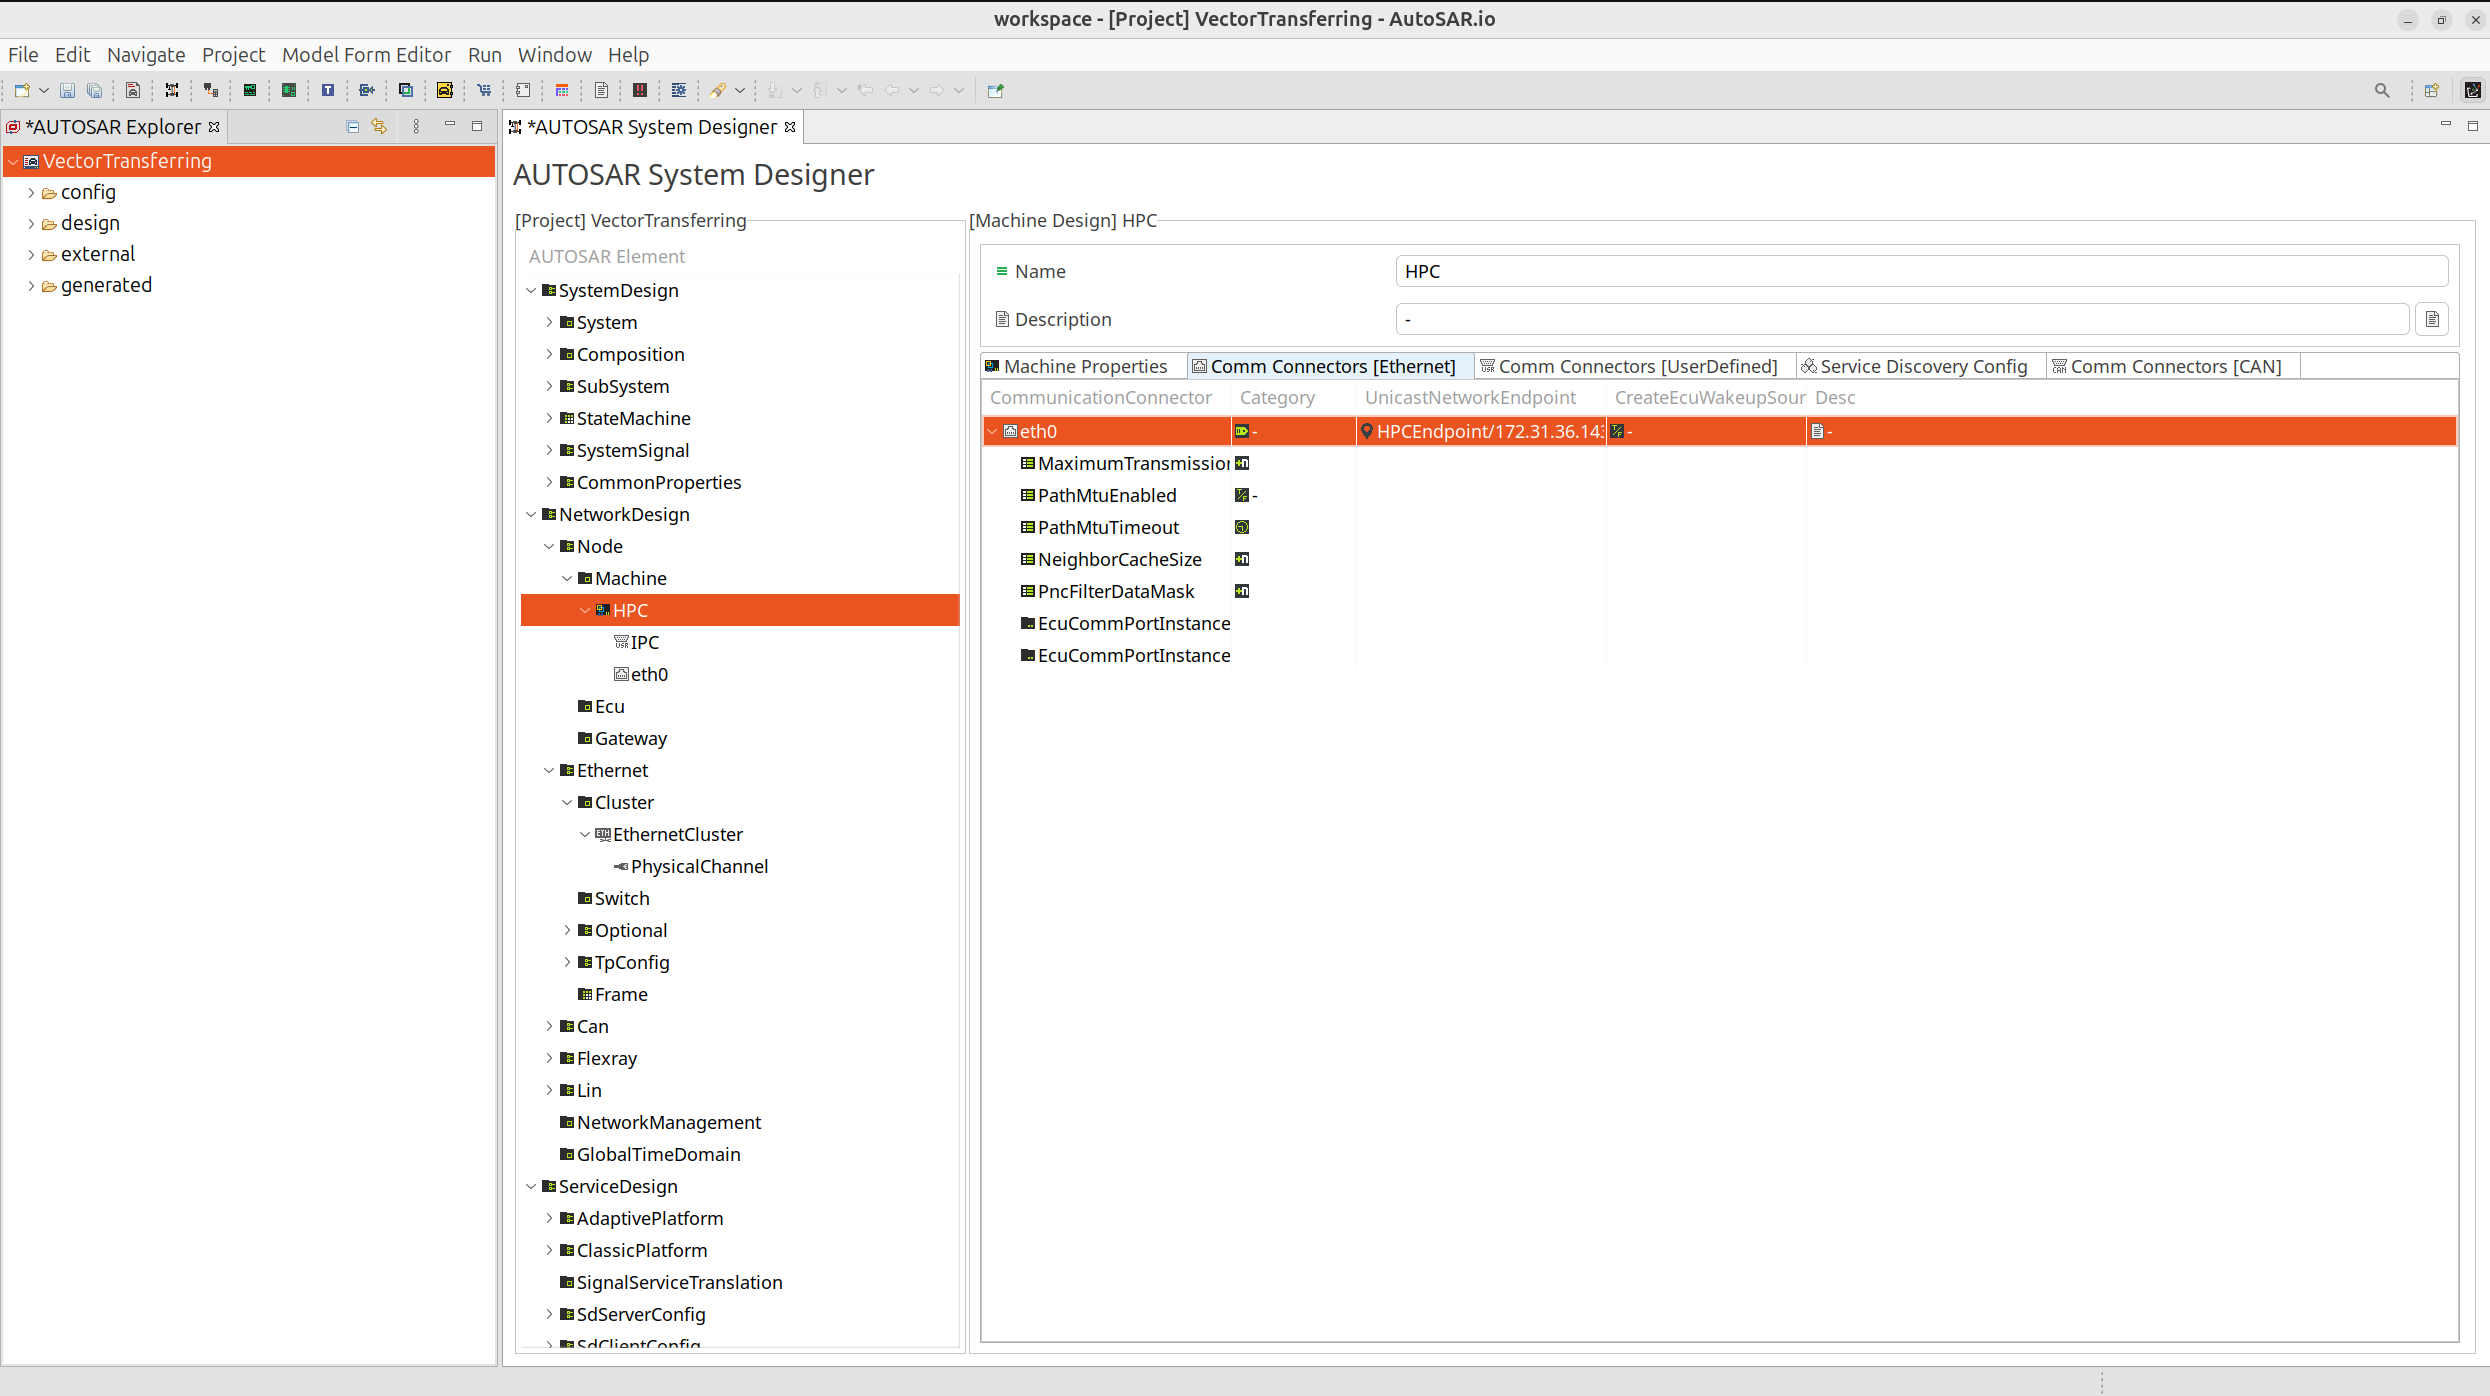
\includegraphics[width=0.75\textwidth]{Images/chap3/image_methodology/machineDesign/addEthMachineDesign.png}
    \vspace{0.5cm}
    \caption{Integration of Ethernet Configuration into Machine Design}
    \label{fig:machine_add_eth_design}
\end{figure}

Figure~\ref{fig:machine_add_eth_design} depicts how the HPC machine is linked to its network interface through the eth0 connector in the Machine Design view. This connector is mapped to a unicast endpoint identified as HPCEndpoint with the IPv4 address 172.31.36.143, defining the machine’s network presence within the Adaptive AUTOSAR system. The figure also highlights adjustable communication parameters such as transmission limits and path MTU handling, which allow the network behavior to be adapted while maintaining reliable data exchange at runtime.

% Configure Service Discovery in Machine Design
\begin{figure}[H]
    \centering
    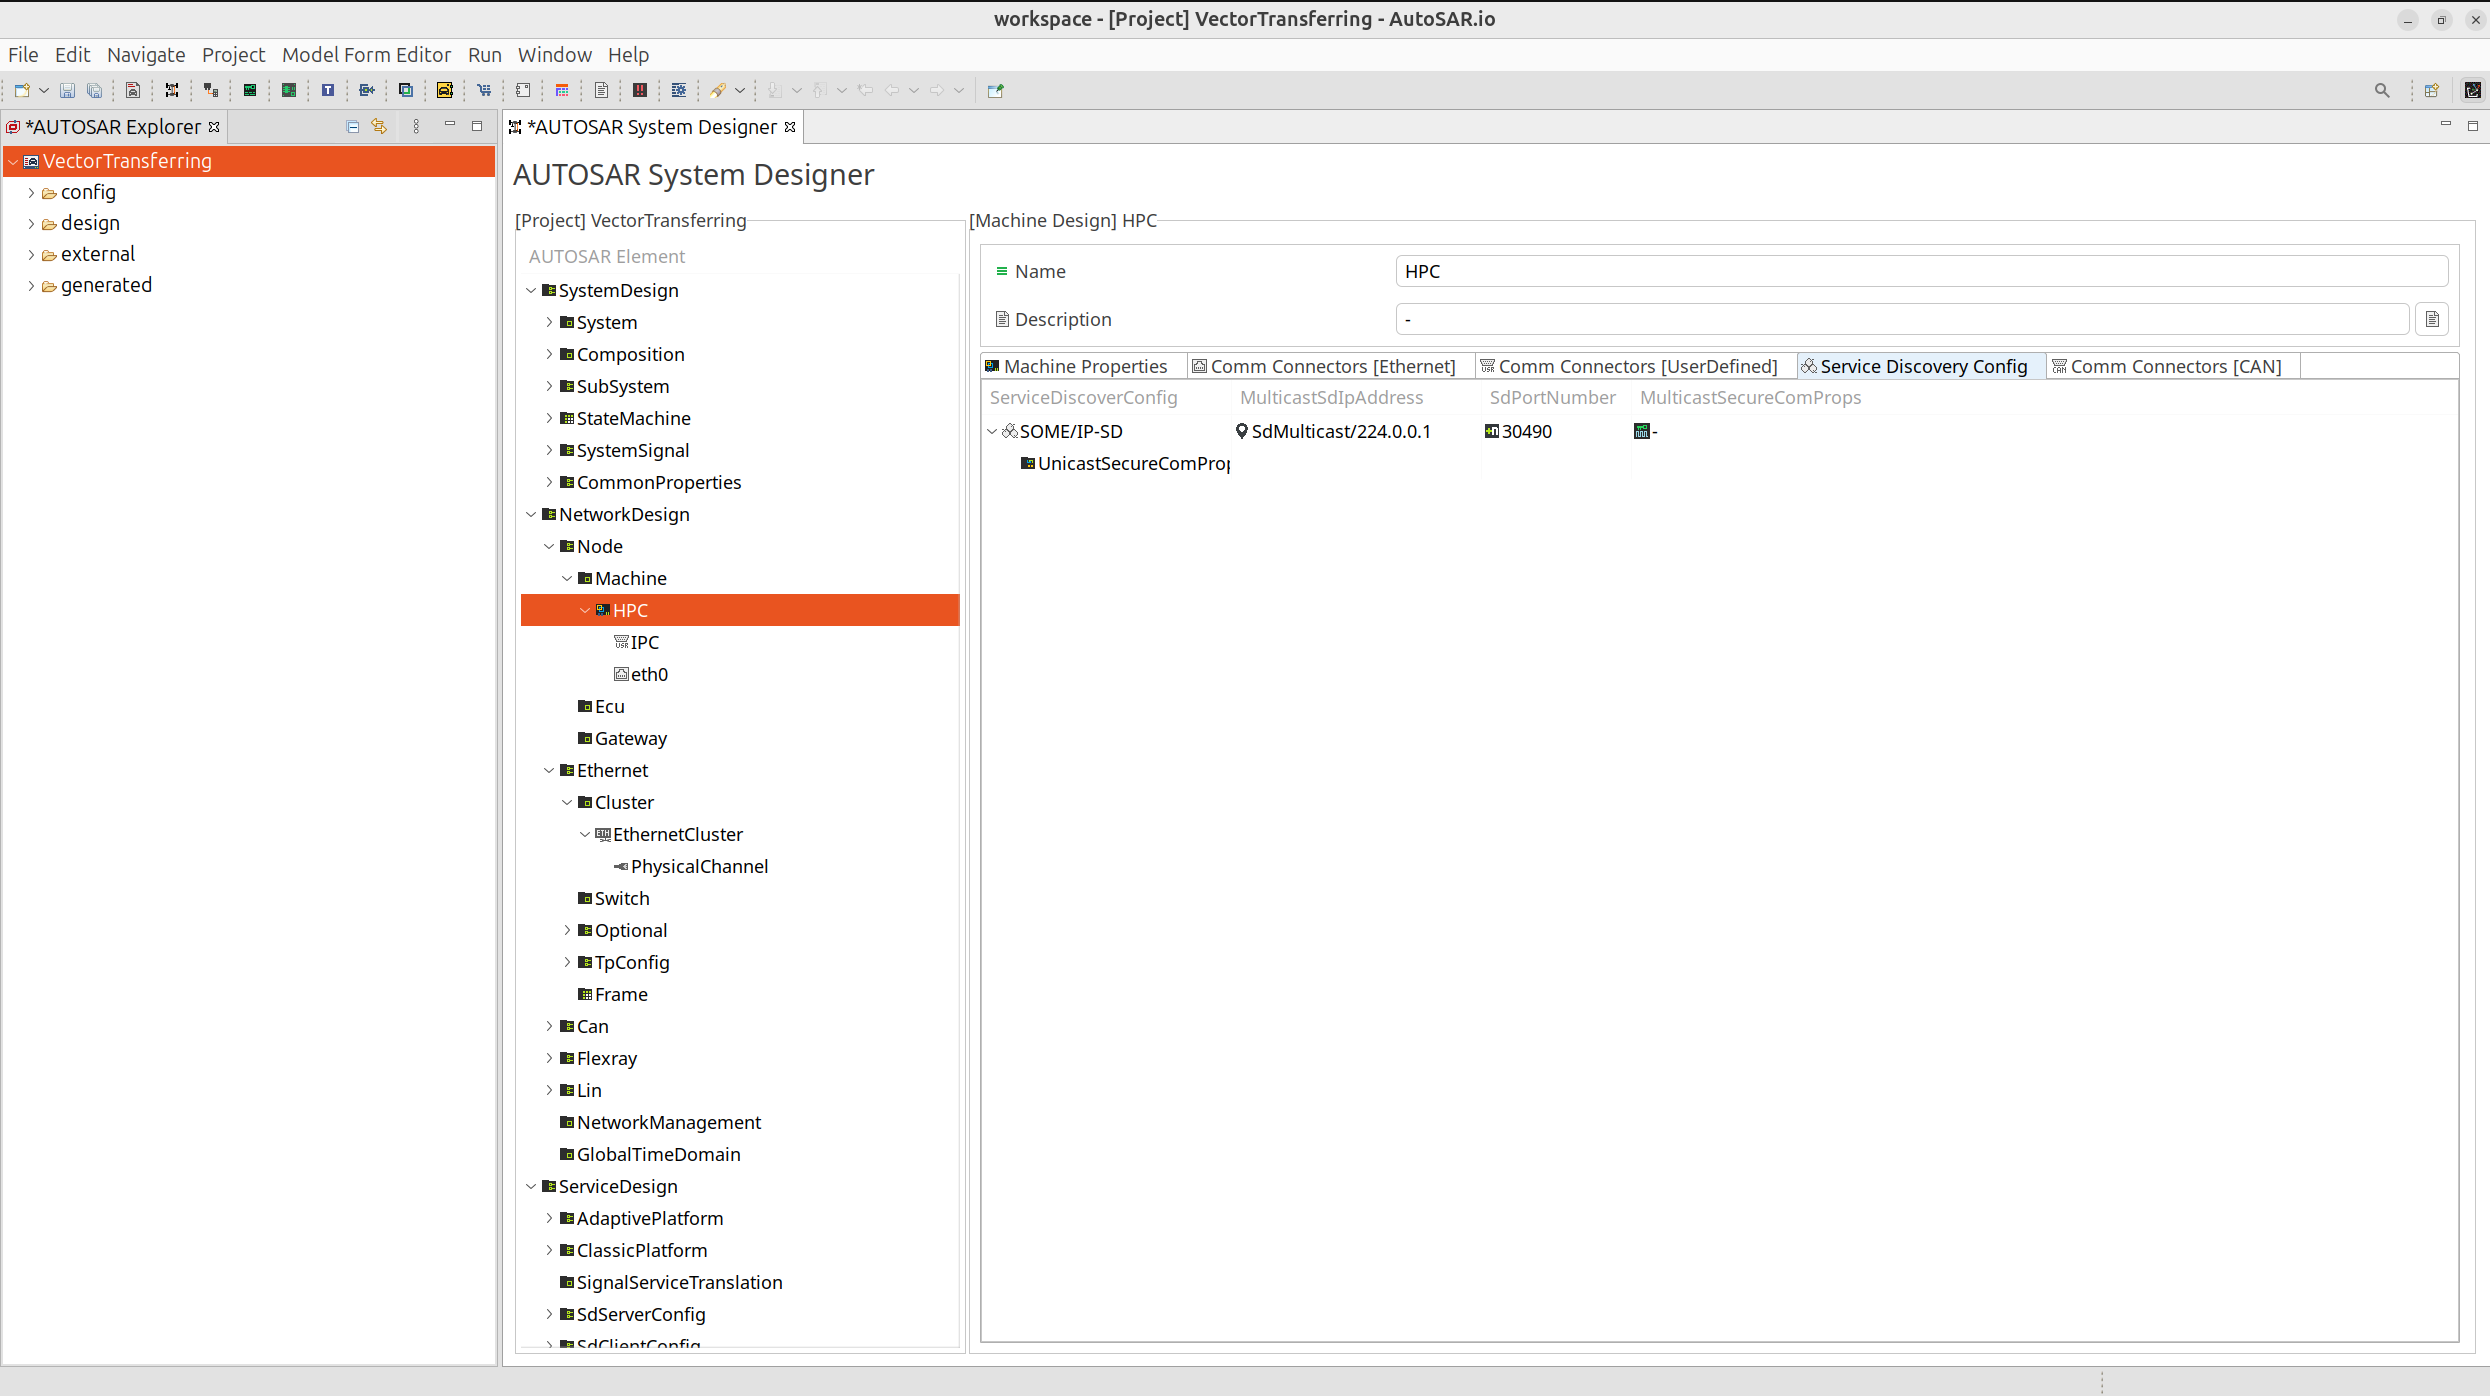
\includegraphics[width=0.75\textwidth]{Images/chap3/image_methodology/machineDesign/addSdConfigMachineDesign.png}
    \vspace{0.5cm}
    \caption{Service Discovery Configuration in Machine Design}
    \label{fig:machine_sd_config}
\end{figure}

Figure~\ref{fig:machine_sd_config} illustrates the Service Discovery setup for the HPC machine within the Machine Design environment. The SOME IP Service Discovery mechanism is configured using the multicast address 224.0.0.1 together with the service discovery port number 30490, which enables applications to announce and detect available services at runtime. This configuration allows dynamic interaction between Adaptive AUTOSAR applications while supporting flexible service availability without relying on static communication bindings.

% Configure Diagnostic Log and Trace (DLT)
\begin{figure}[H]
    \centering
    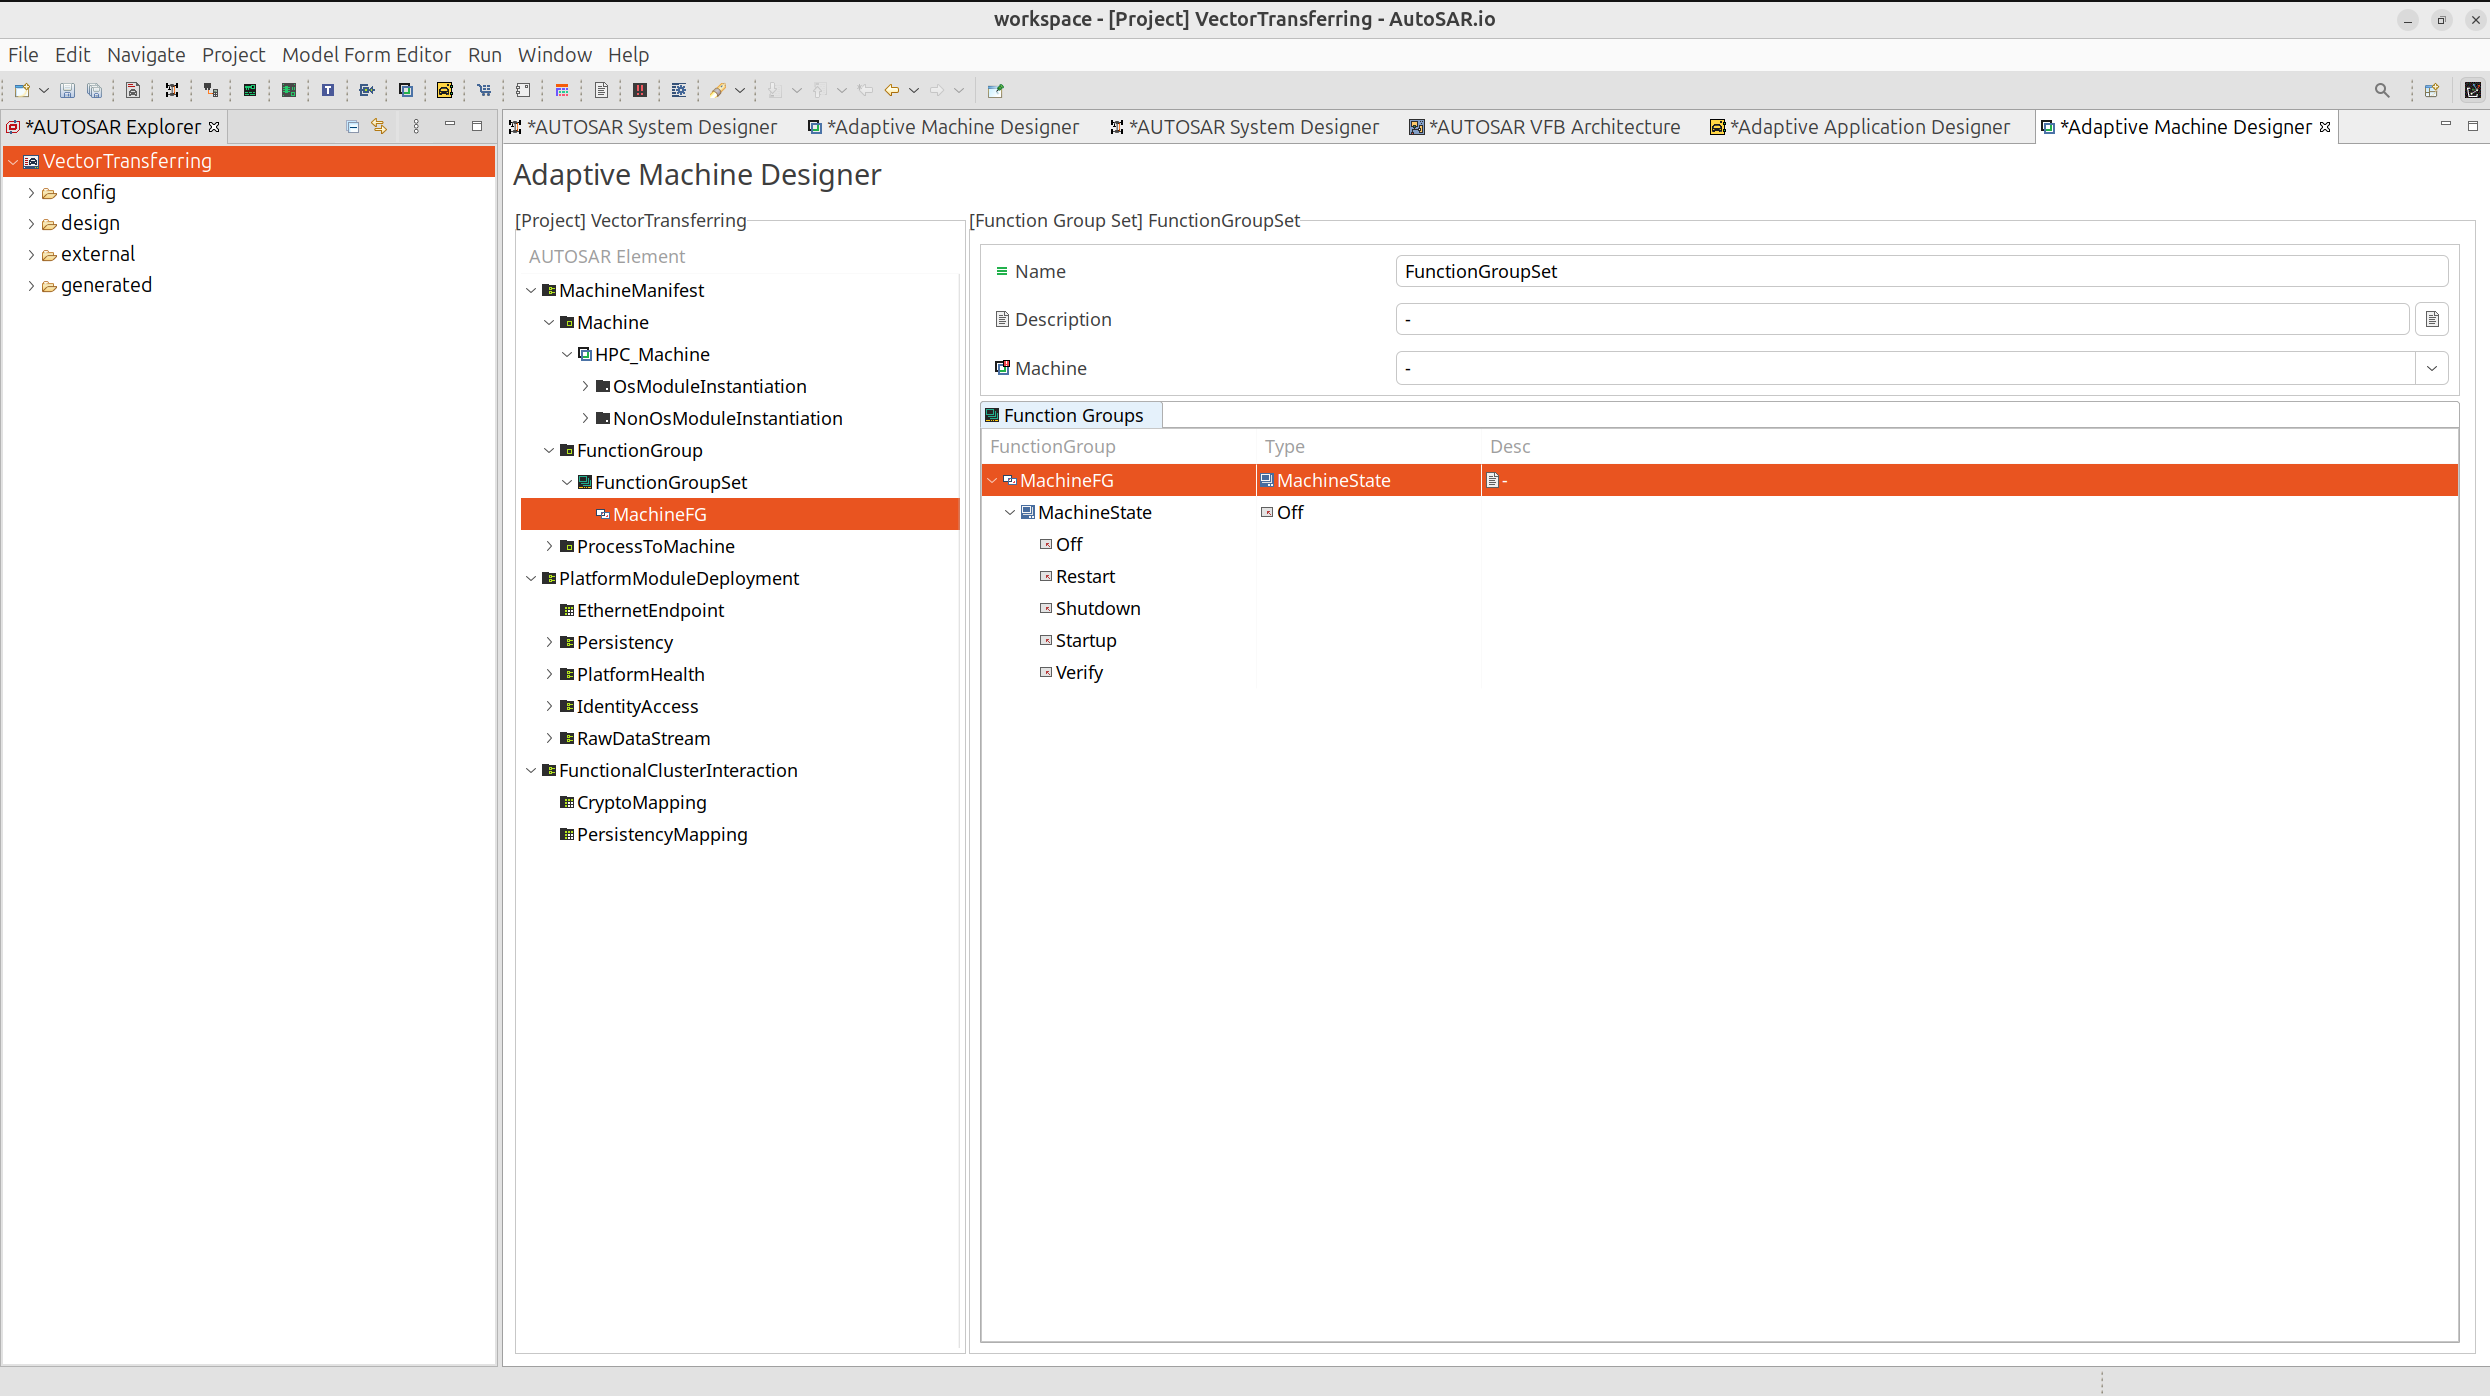
\includegraphics[width=0.75\textwidth]{Images/chap3/image_methodology/machineDesign/configMachineFG.png}
    \vspace{0.5cm}
    \caption{Machine Function Group States Configuration}
    \label{fig:machine_fg_config}
\end{figure}

The figure \ref{fig:machine_fg_config} presents the configuration of the machine function group for the HPC\_Machine in the Adaptive Machine Designer. A function group named MachineFG is defined with the MachineState type, which includes states such as Off, Startup, Verify, Restart, and Shutdown. This configuration governs how the machine progresses through its operational lifecycle, ensuring that platform services and applications are activated and controlled according to well defined system states during runtime execution.

% Final Machine Manifest
\begin{figure}[H]
    \centering
    
\includegraphics[width=0.75\textwidth]{Images/chap3/image_methodology/machineDesign/machineManifest.png}
    \vspace{0.5cm}
    \caption{Machine Manifest for Adaptive AUTOSAR Deployment}
    \label{fig:machine_manifest}
\end{figure}

The figure \ref{fig:machine_manifest} presents the Machine Manifest of the HPC\_Machine as defined in the Adaptive Machine Designer. This manifest consolidates all machine level configurations by referencing the previously defined Machine Design, including the SOME/IP Service Discovery endpoint with the multicast address 224.0.0.1 and port 30490, as well as the Ethernet connector bound to the eth0 interface. In addition, user defined connectors and inter process communication settings are integrated, forming a complete description of the communication capabilities of the target machine.

Furthermore, the manifest specifies essential execution and platform related properties such as trusted platform execution mode, default application timeout, and processor configuration. The processor section defines the available CPU resources and core assignment, while function group and process to machine mappings establish how applications are bound to machine states at runtime. By combining communication, execution, and lifecycle information into a single artifact, the Machine Manifest serves as the final deployment blueprint for Adaptive AUTOSAR applications.

% Configure Operating System platform module
\begin{figure}[H]
    \centering
    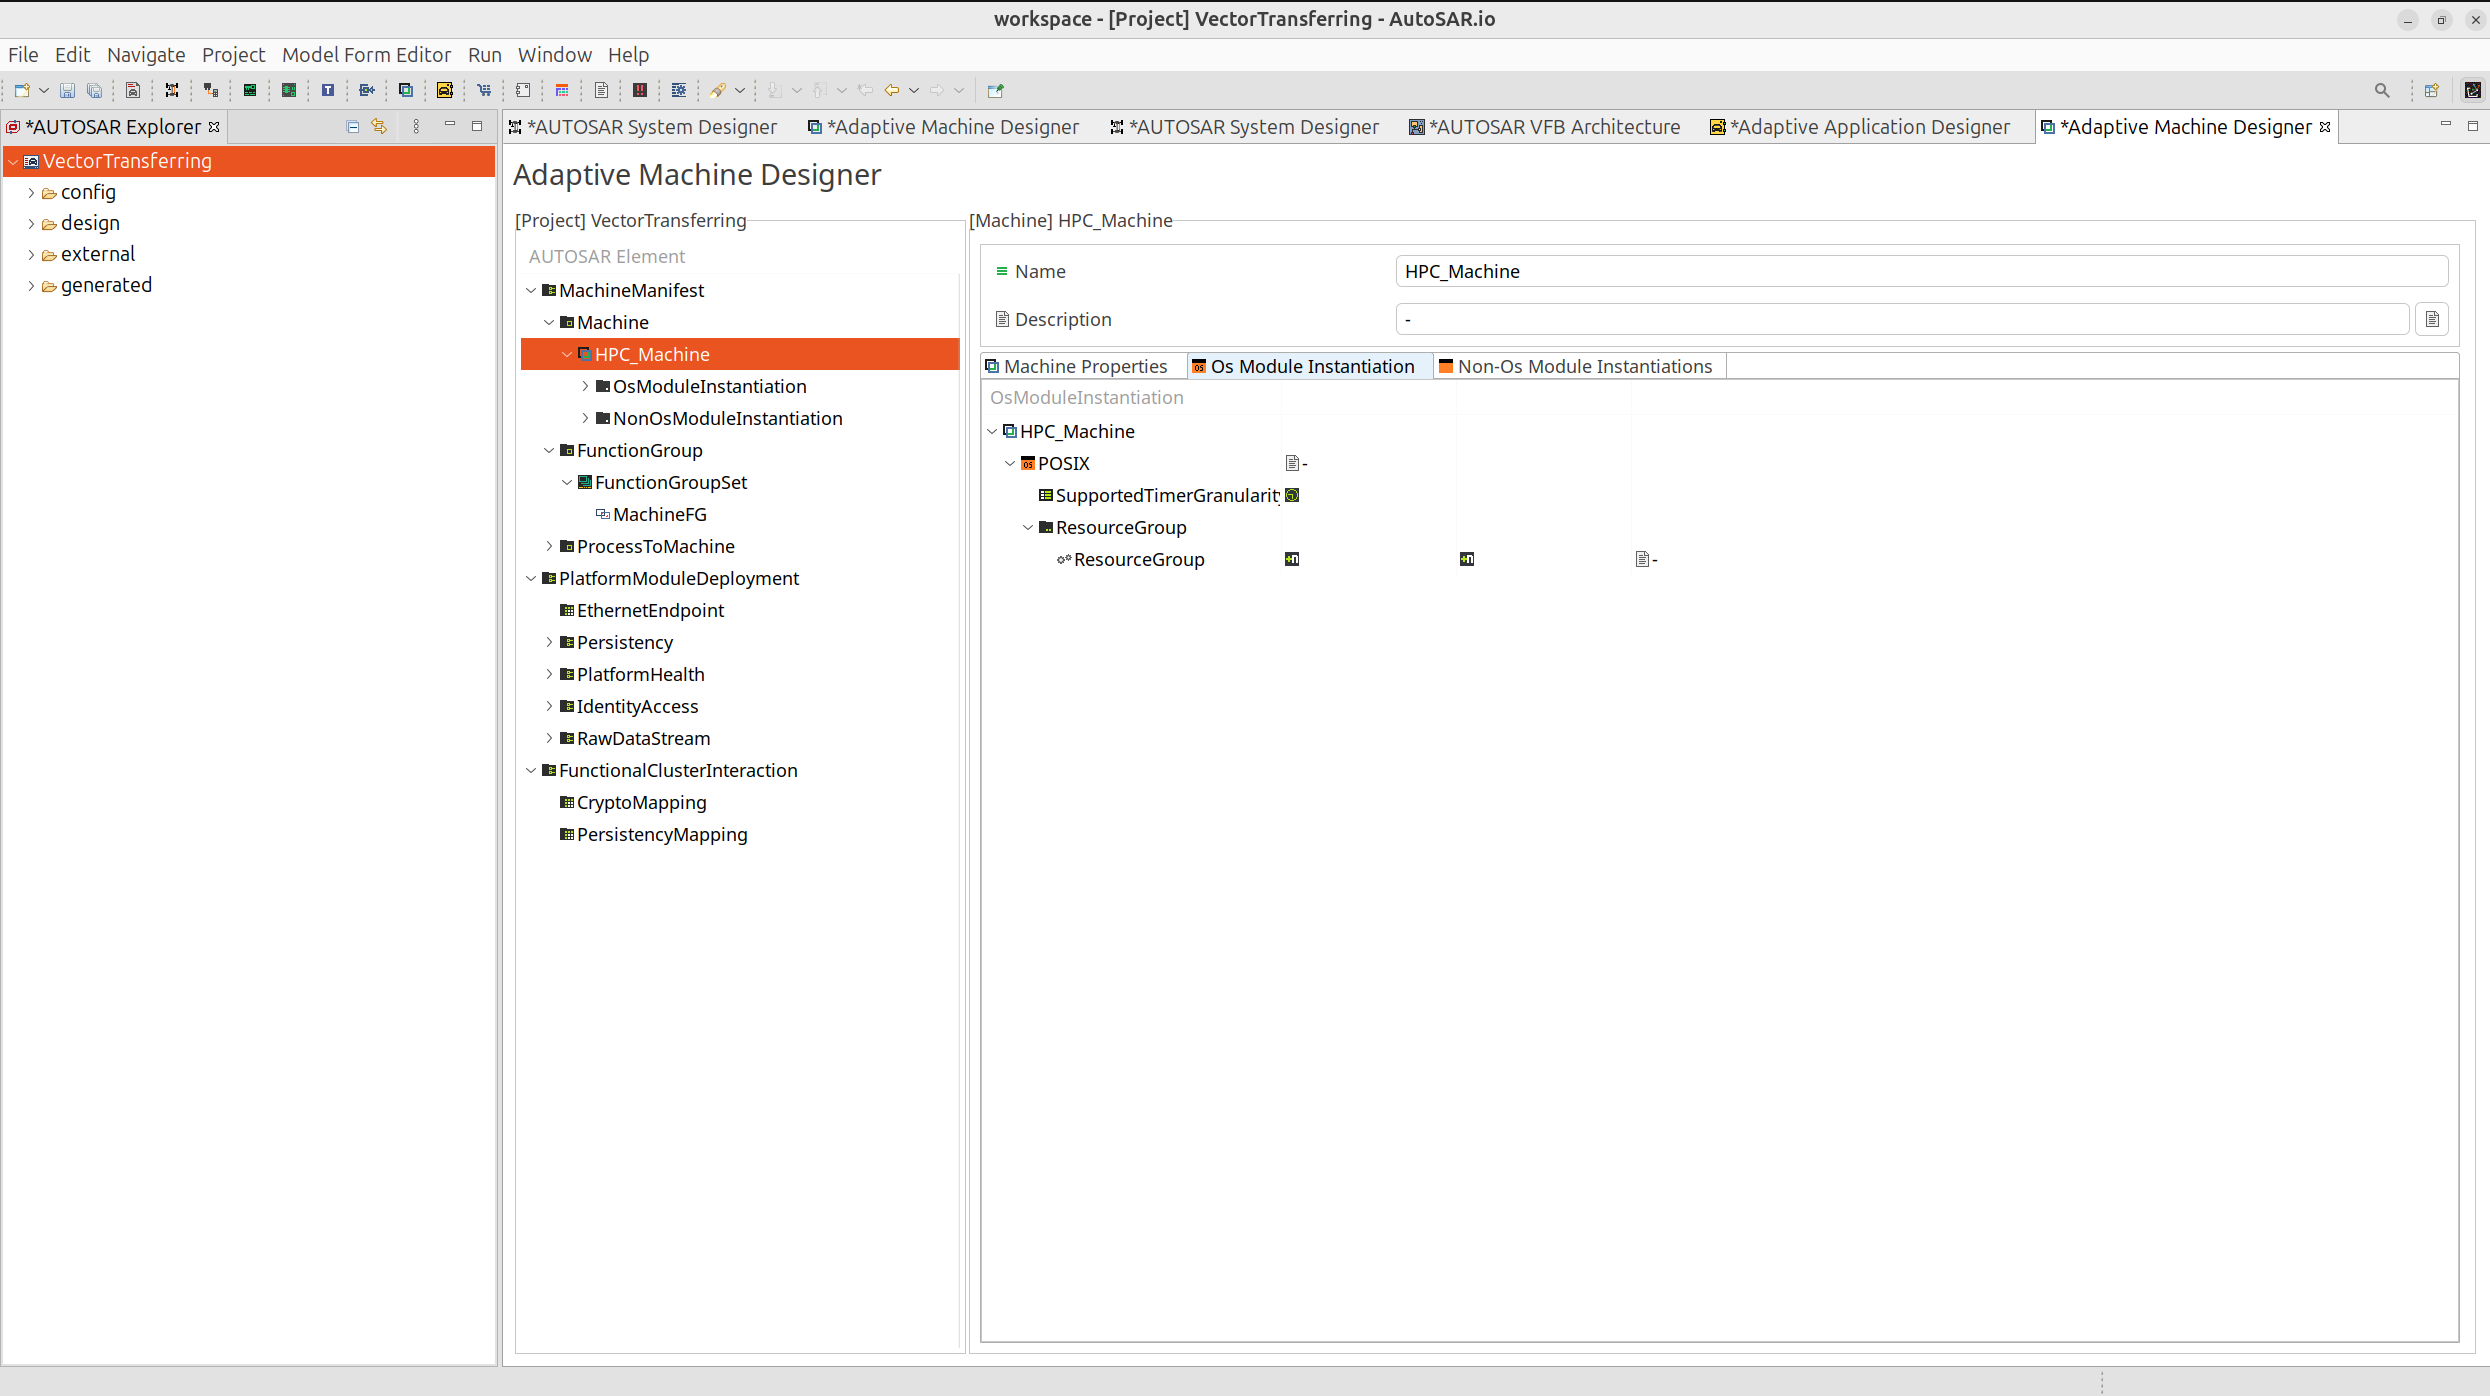
\includegraphics[width=0.75\textwidth]{Images/chap3/image_methodology/machineDesign/configOSModule.png}
    \vspace{0.5cm}
    \caption{Operating System Platform Module Configuration}
    \label{fig:machine_os_module}
\end{figure}

Figure~\ref{fig:machine_os_module} shows the operating system platform module configuration for the target machine named HPC\_Machine in the Adaptive Machine Designer. The POSIX based operating system module is instantiated to define the execution environment for Adaptive AUTOSAR applications, including supported timer granularity and resource group settings. This configuration establishes the fundamental runtime services required for process scheduling and resource management on the target machine.

% Configure non-OS platform modules
\begin{figure}[H]
    \centering
    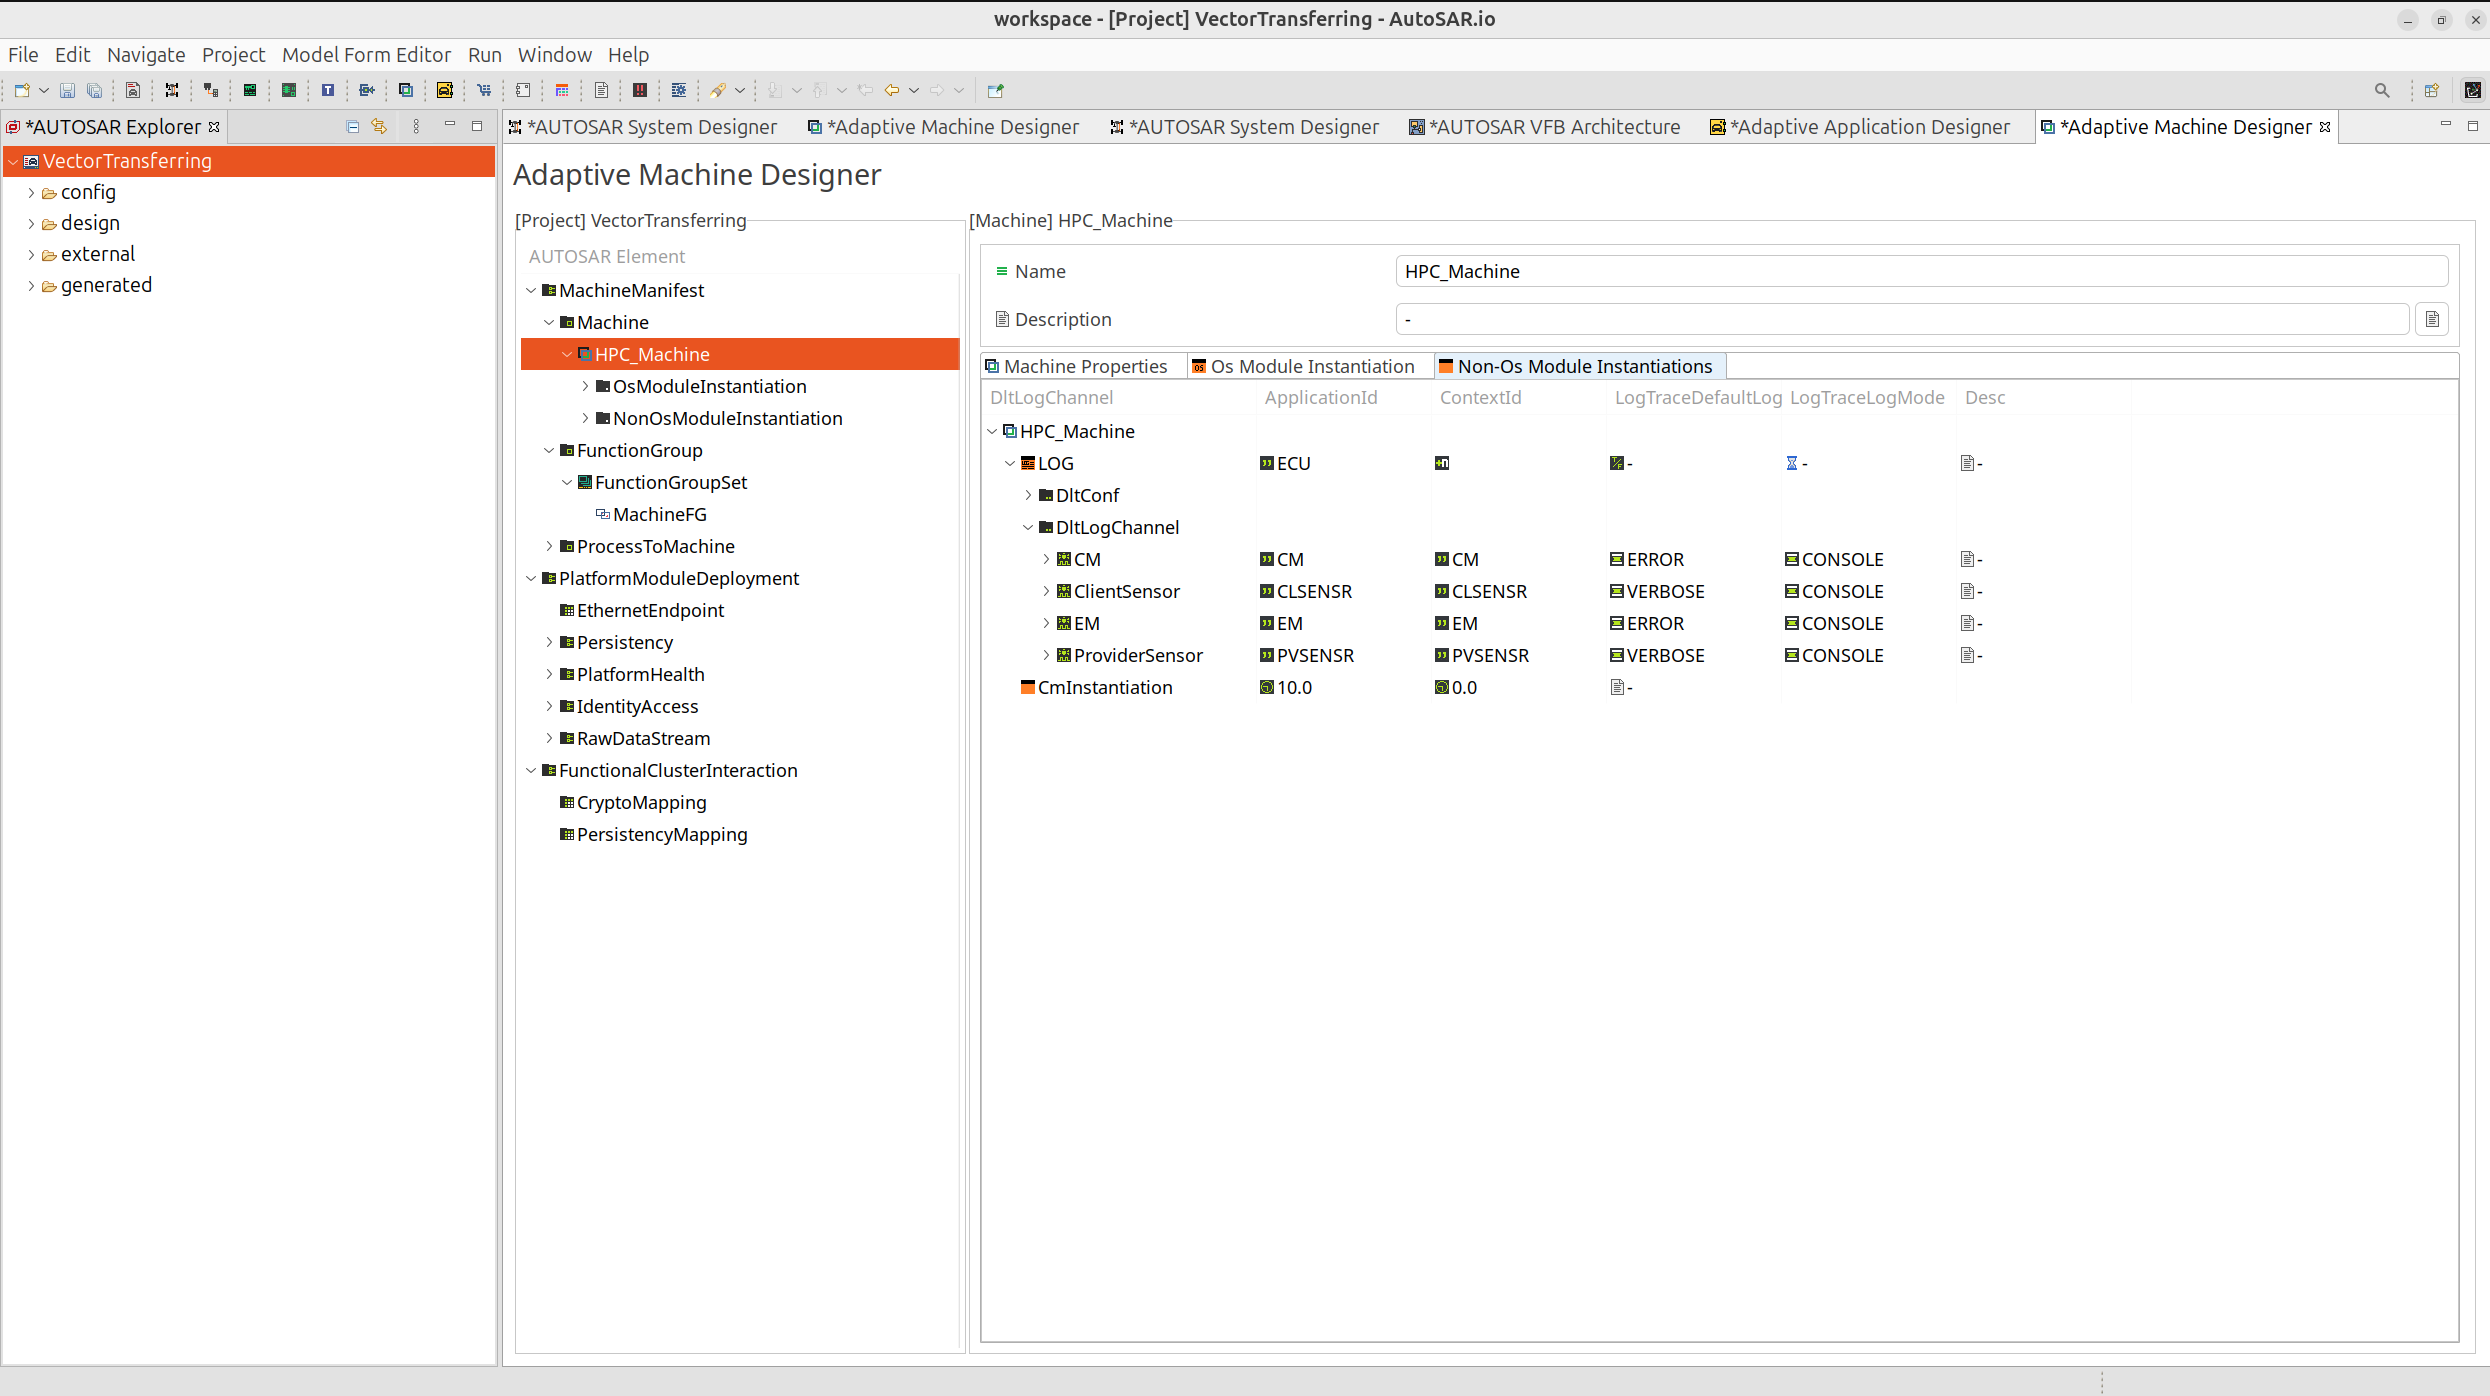
\includegraphics[width=0.75\textwidth]{Images/chap3/image_methodology/machineDesign/configNonOS.png}
    \vspace{0.5cm}
    \caption{Configuration of Non-OS Platform Modules}
    \label{fig:machine_non_os_module}
\end{figure}

Figure~\ref{fig:machine_non_os_module} presents the configuration of Diagnostic Log and Trace for the HPC\_Machine in the Adaptive Machine Designer. Several log channels are defined for different software entities, including ECU, ClientSensor, EM, and ProviderSensor, each mapped to a distinct ApplicationId and ContextId. Log levels such as ERROR and VERBOSE are specified, and the output is directed to the console, allowing developers to monitor application execution and diagnose runtime behavior.

In addition, the configuration highlights the role of CMInstantiation, which represents the Communication Management daemon responsible for inter process communication on the Adaptive Platform. This daemon enables different processes to exchange messages and supports the transport of diagnostic data between applications and platform services. By instantiating the communication manager at the machine level, the system ensures that logging, tracing, and service communication operate coherently across all running processes.

\subsubsection{Service Interface Design and Mapping}

% Define data types for service interfaces
\begin{figure}[H]
    \centering
    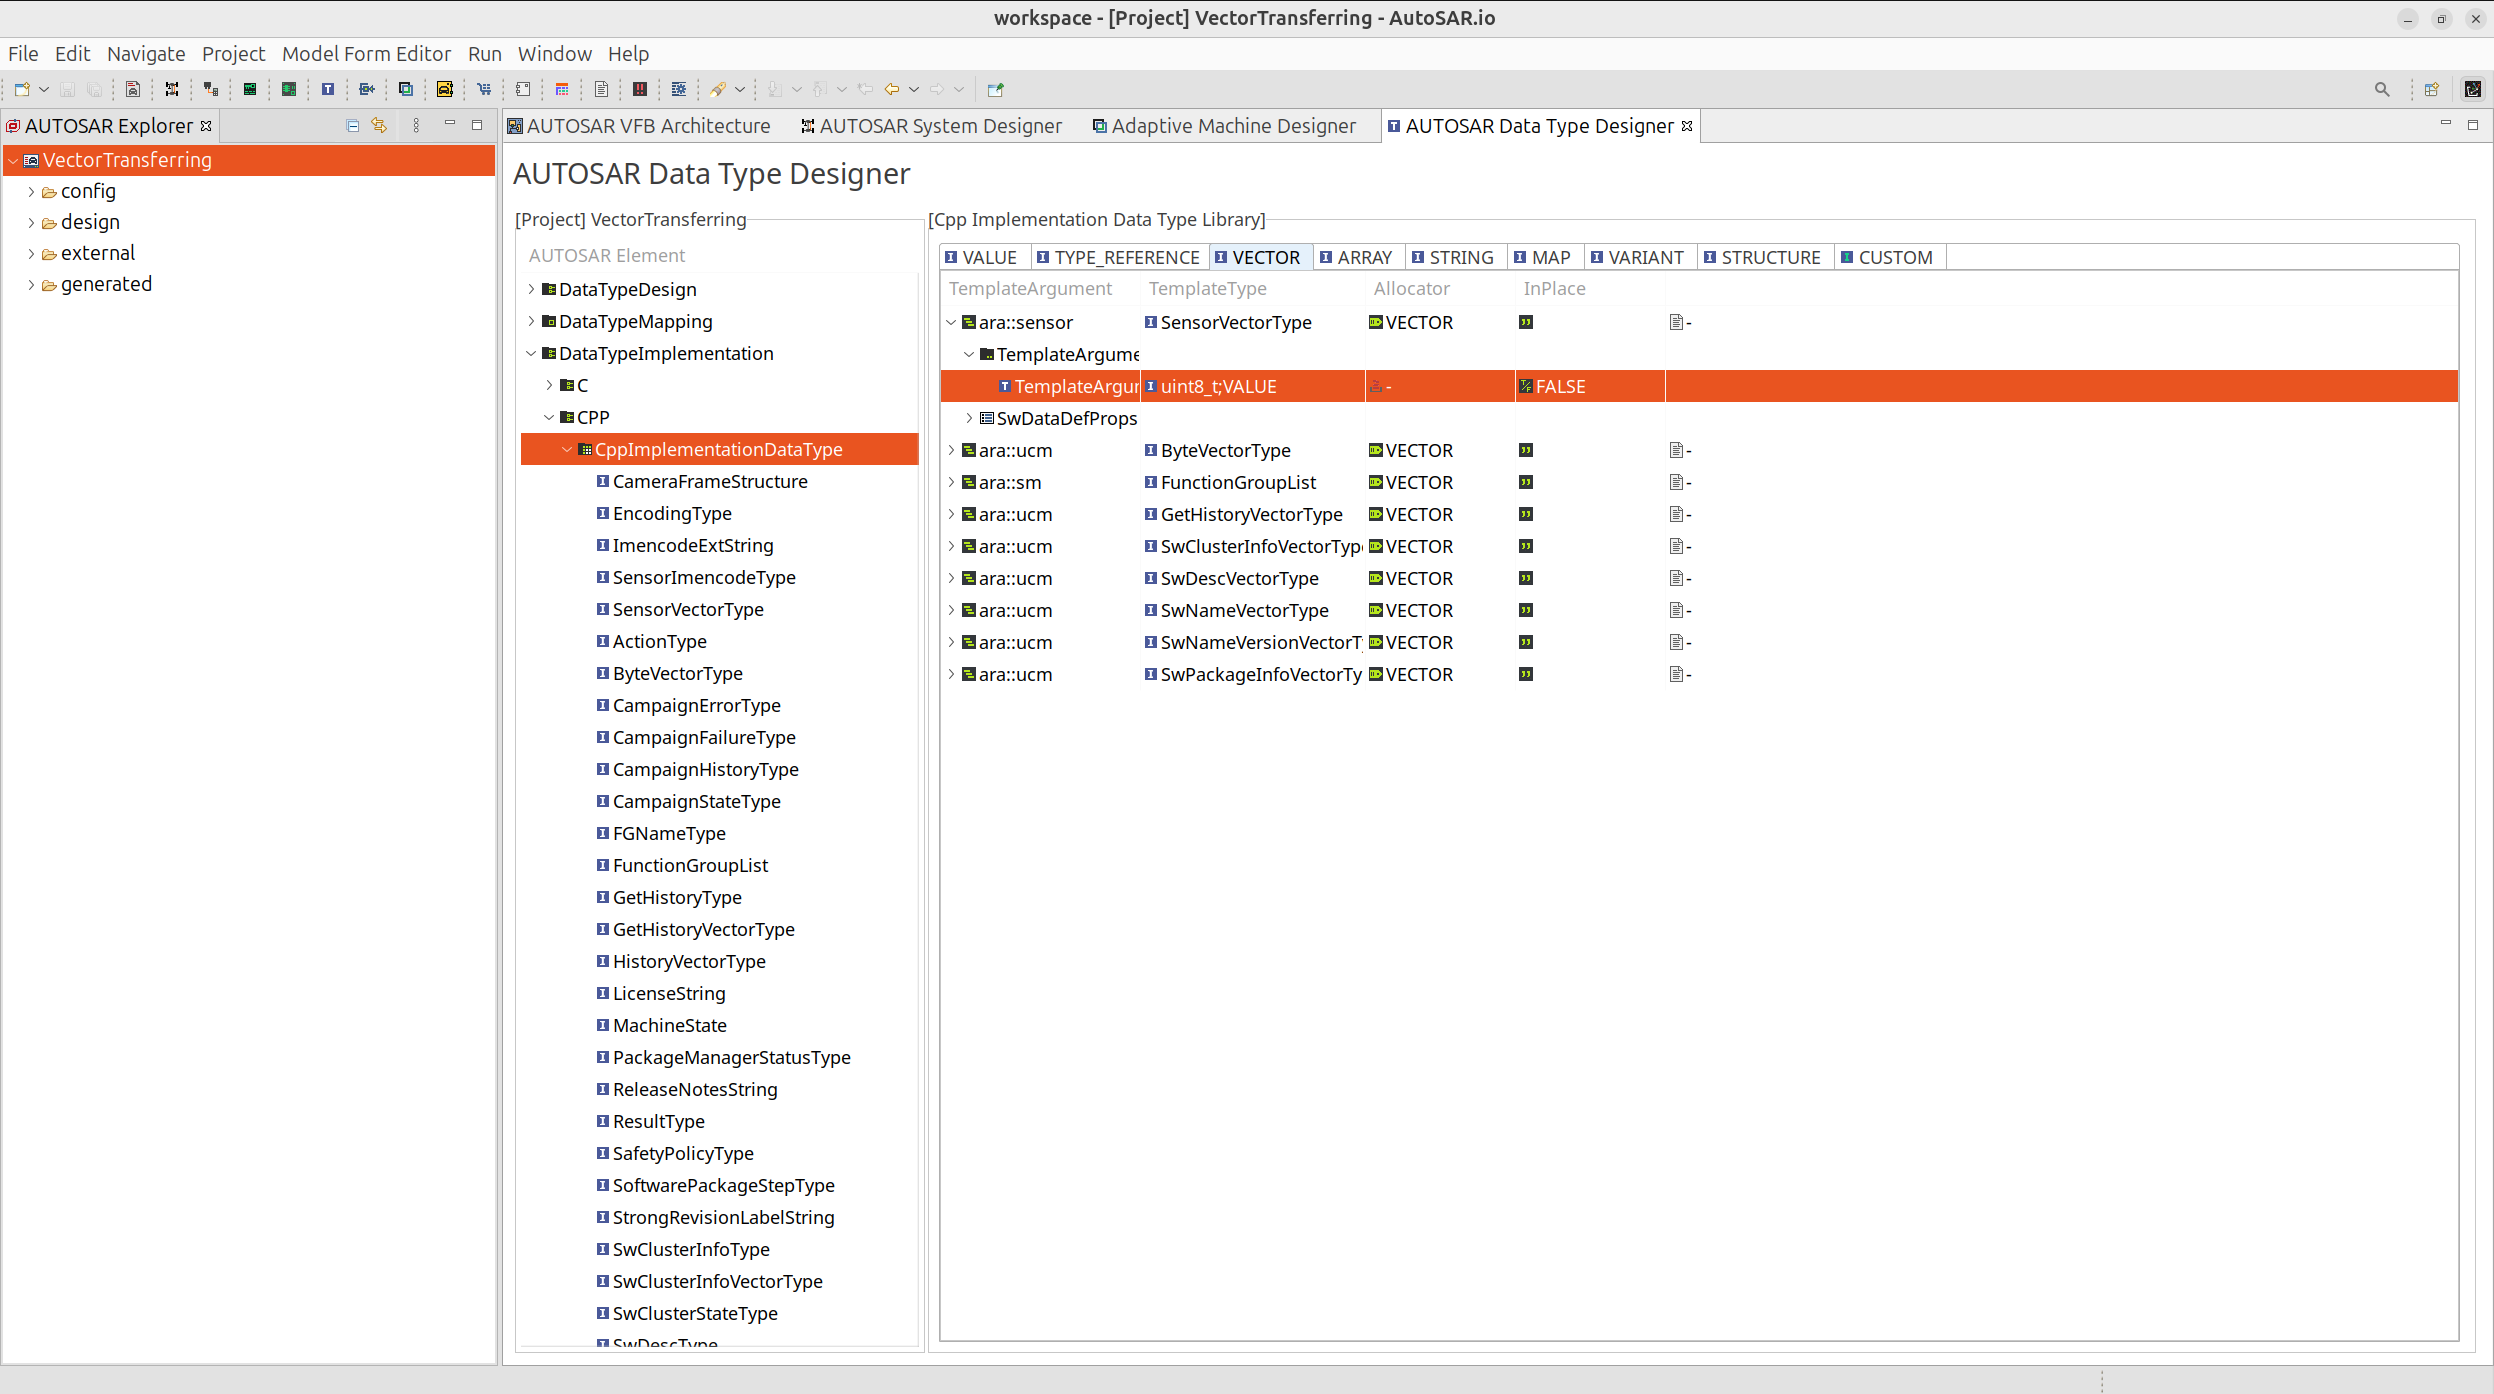
\includegraphics[width=0.75\textwidth]{Images/chap3/image_methodology/serviceInterfaceDesign/dataType.png}
    \vspace{0.5cm}
    \caption{Definition of Data Types for Service Interfaces}
    \label{fig:service_datatype}
\end{figure}

The figure~\ref{fig:service_datatype} shows the specification of C++ data types used to support service interfaces in the Adaptive AUTOSAR environment. Several vector based types are defined using template arguments, where primitive elements such as \texttt{uint8\_t} are combined to represent structured service data. These type definitions provide a clear and reusable foundation for data exchange between service providers and consumers, ensuring consistency and type safety during service oriented communication.

% Define service interface
\begin{figure}[H]
    \centering
    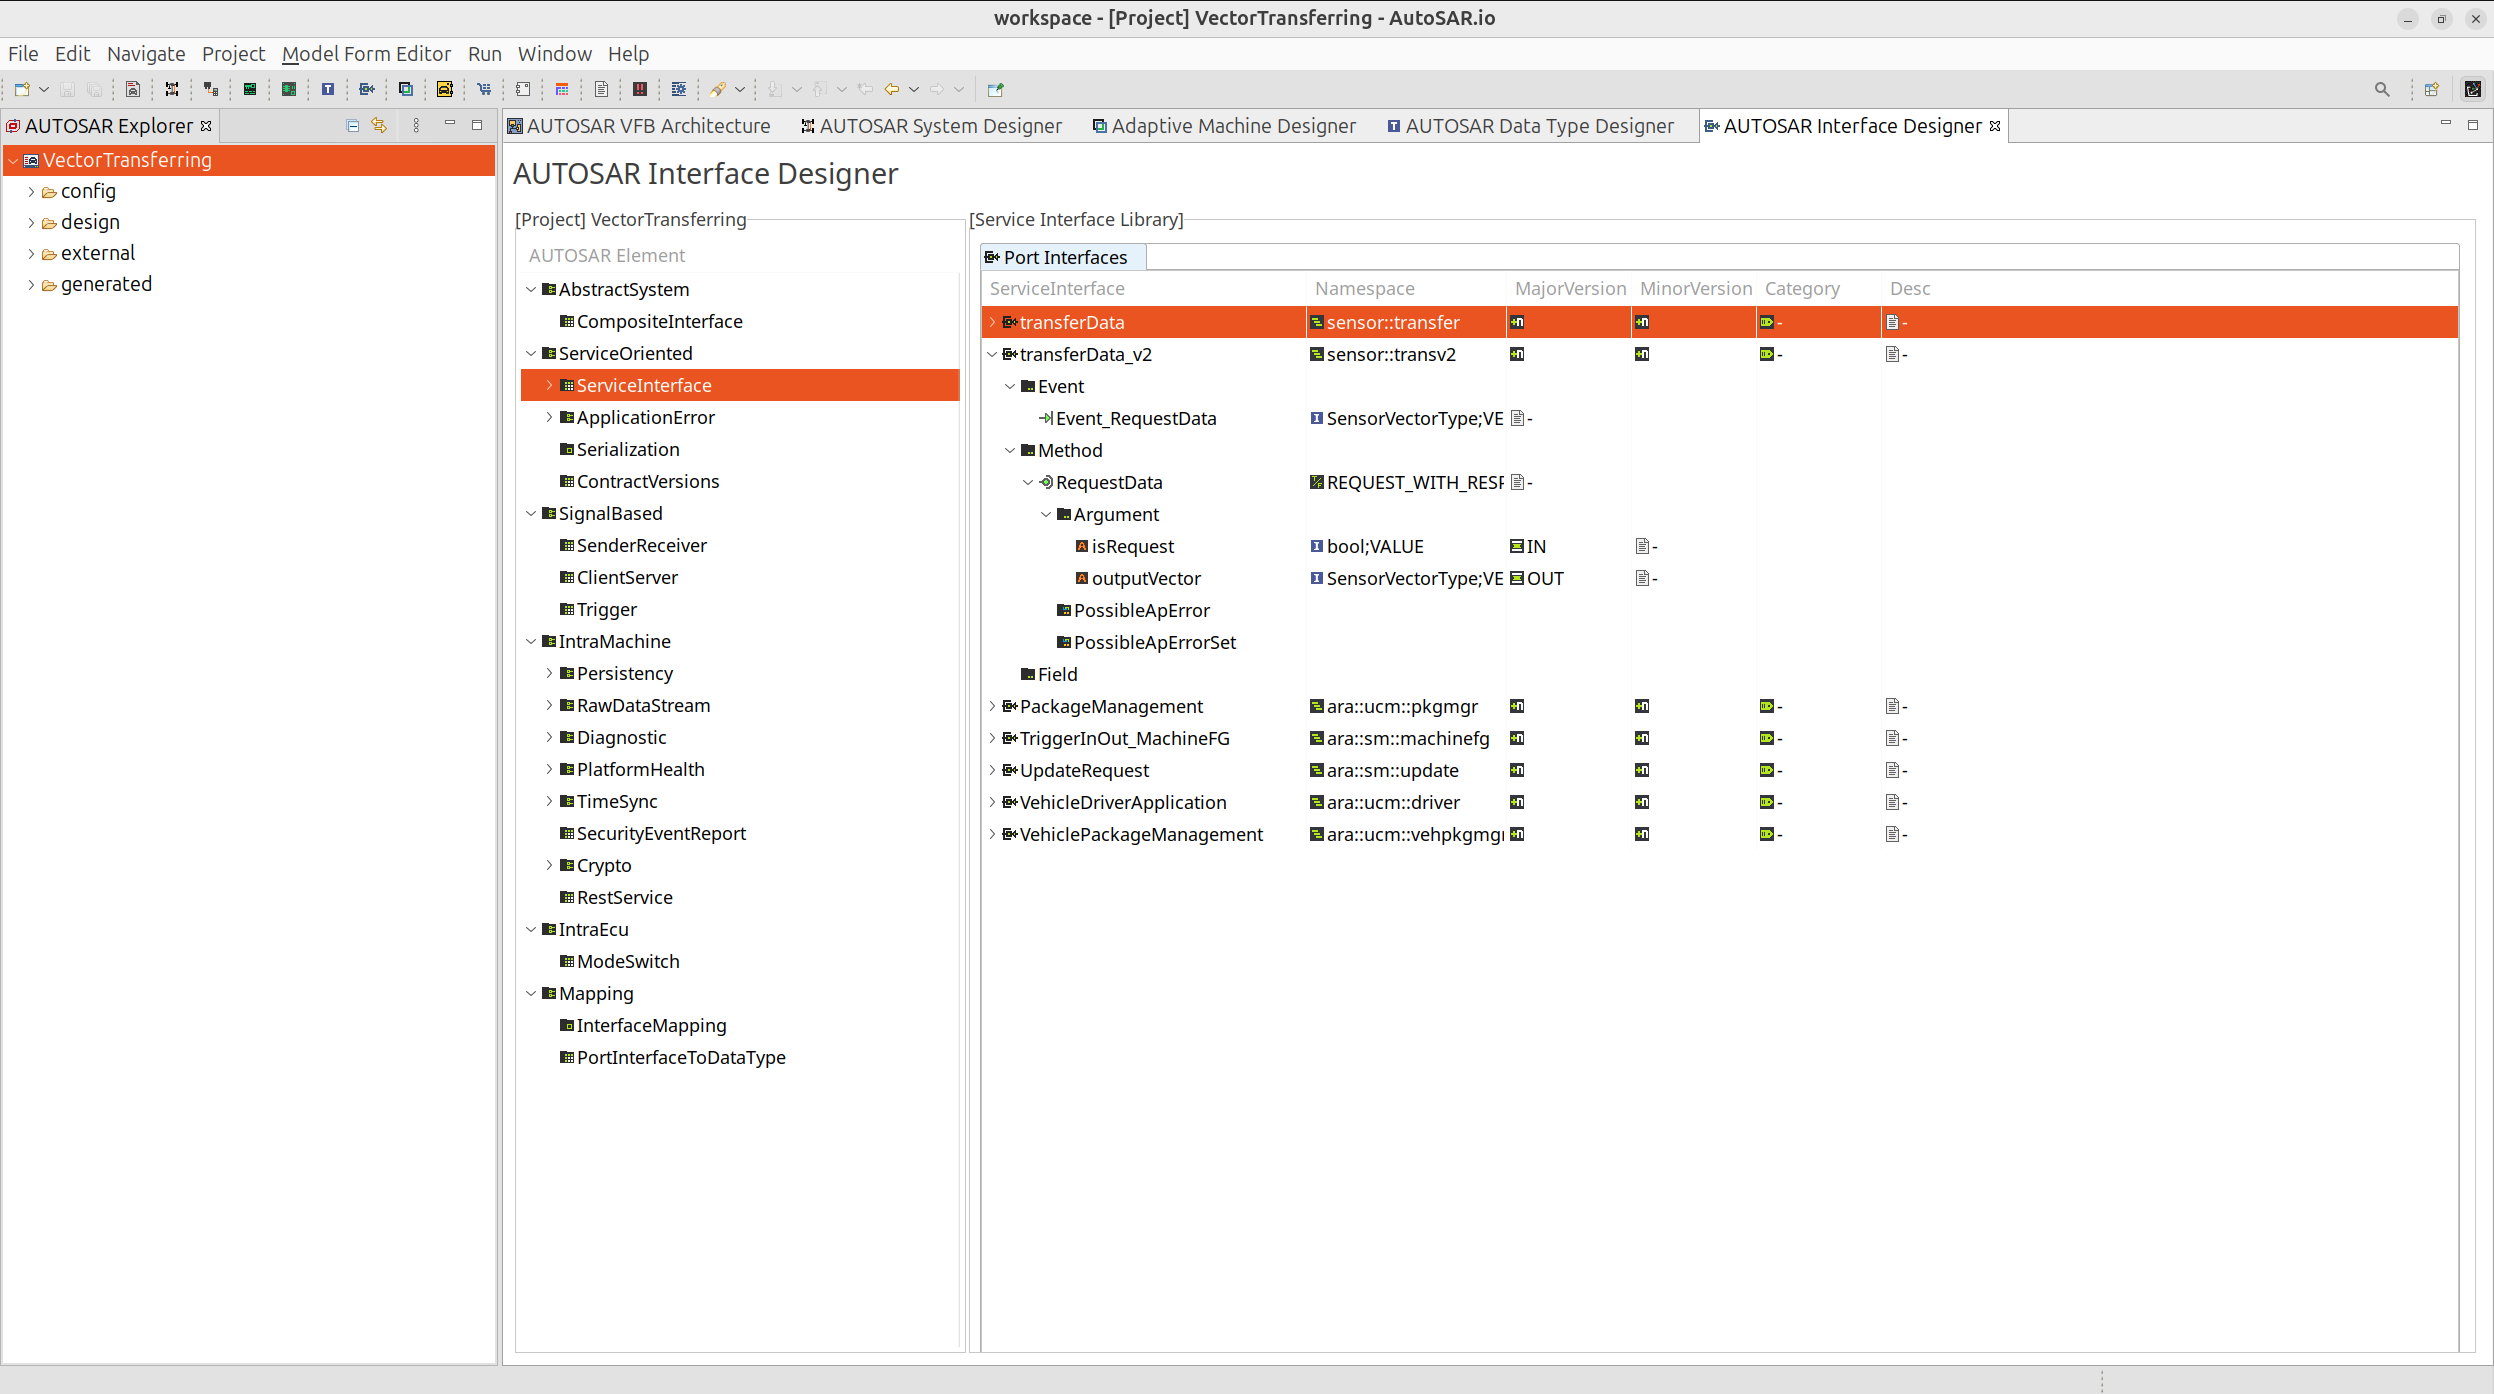
\includegraphics[width=0.75\textwidth]{Images/chap3/image_methodology/serviceInterfaceDesign/defineServiceInterface.png}
    \vspace{0.5cm}
    \caption{Service Interface Definition in Adaptive AUTOSAR}
    \label{fig:service_interface_definition}
\end{figure}

Figure~\ref{fig:service_interface_definition} illustrates the definition of a service oriented interface in the AUTOSAR Interface Designer. The service interface named \texttt{transferData\_v2} is specified within the \texttt{sensor::transv2} namespace and versioned to support interface evolution. It exposes both an event and a method, where the event enables asynchronous notification of data availability, while the method defines a request response interaction pattern for controlled data transmission between applications.

In addition, the interface description includes detailed method arguments and data flow directions. The \texttt{RequestData} method accepts an input parameter that influences the request behavior and produces an output vector based on the previously defined sensor data type. The event is associated with the same data representation (\texttt{Event\_RequestData}), allowing consumers to receive updates without explicitly issuing a request. Possible application errors are also declared to handle exceptional conditions during execution. As shown in Figure~\ref{fig:service_interface_definition}, this interface design supports both reactive and on demand communication between service providers and consumers in the Adaptive AUTOSAR system.


% Service deployment configuration
\begin{figure}[H]
    \centering
    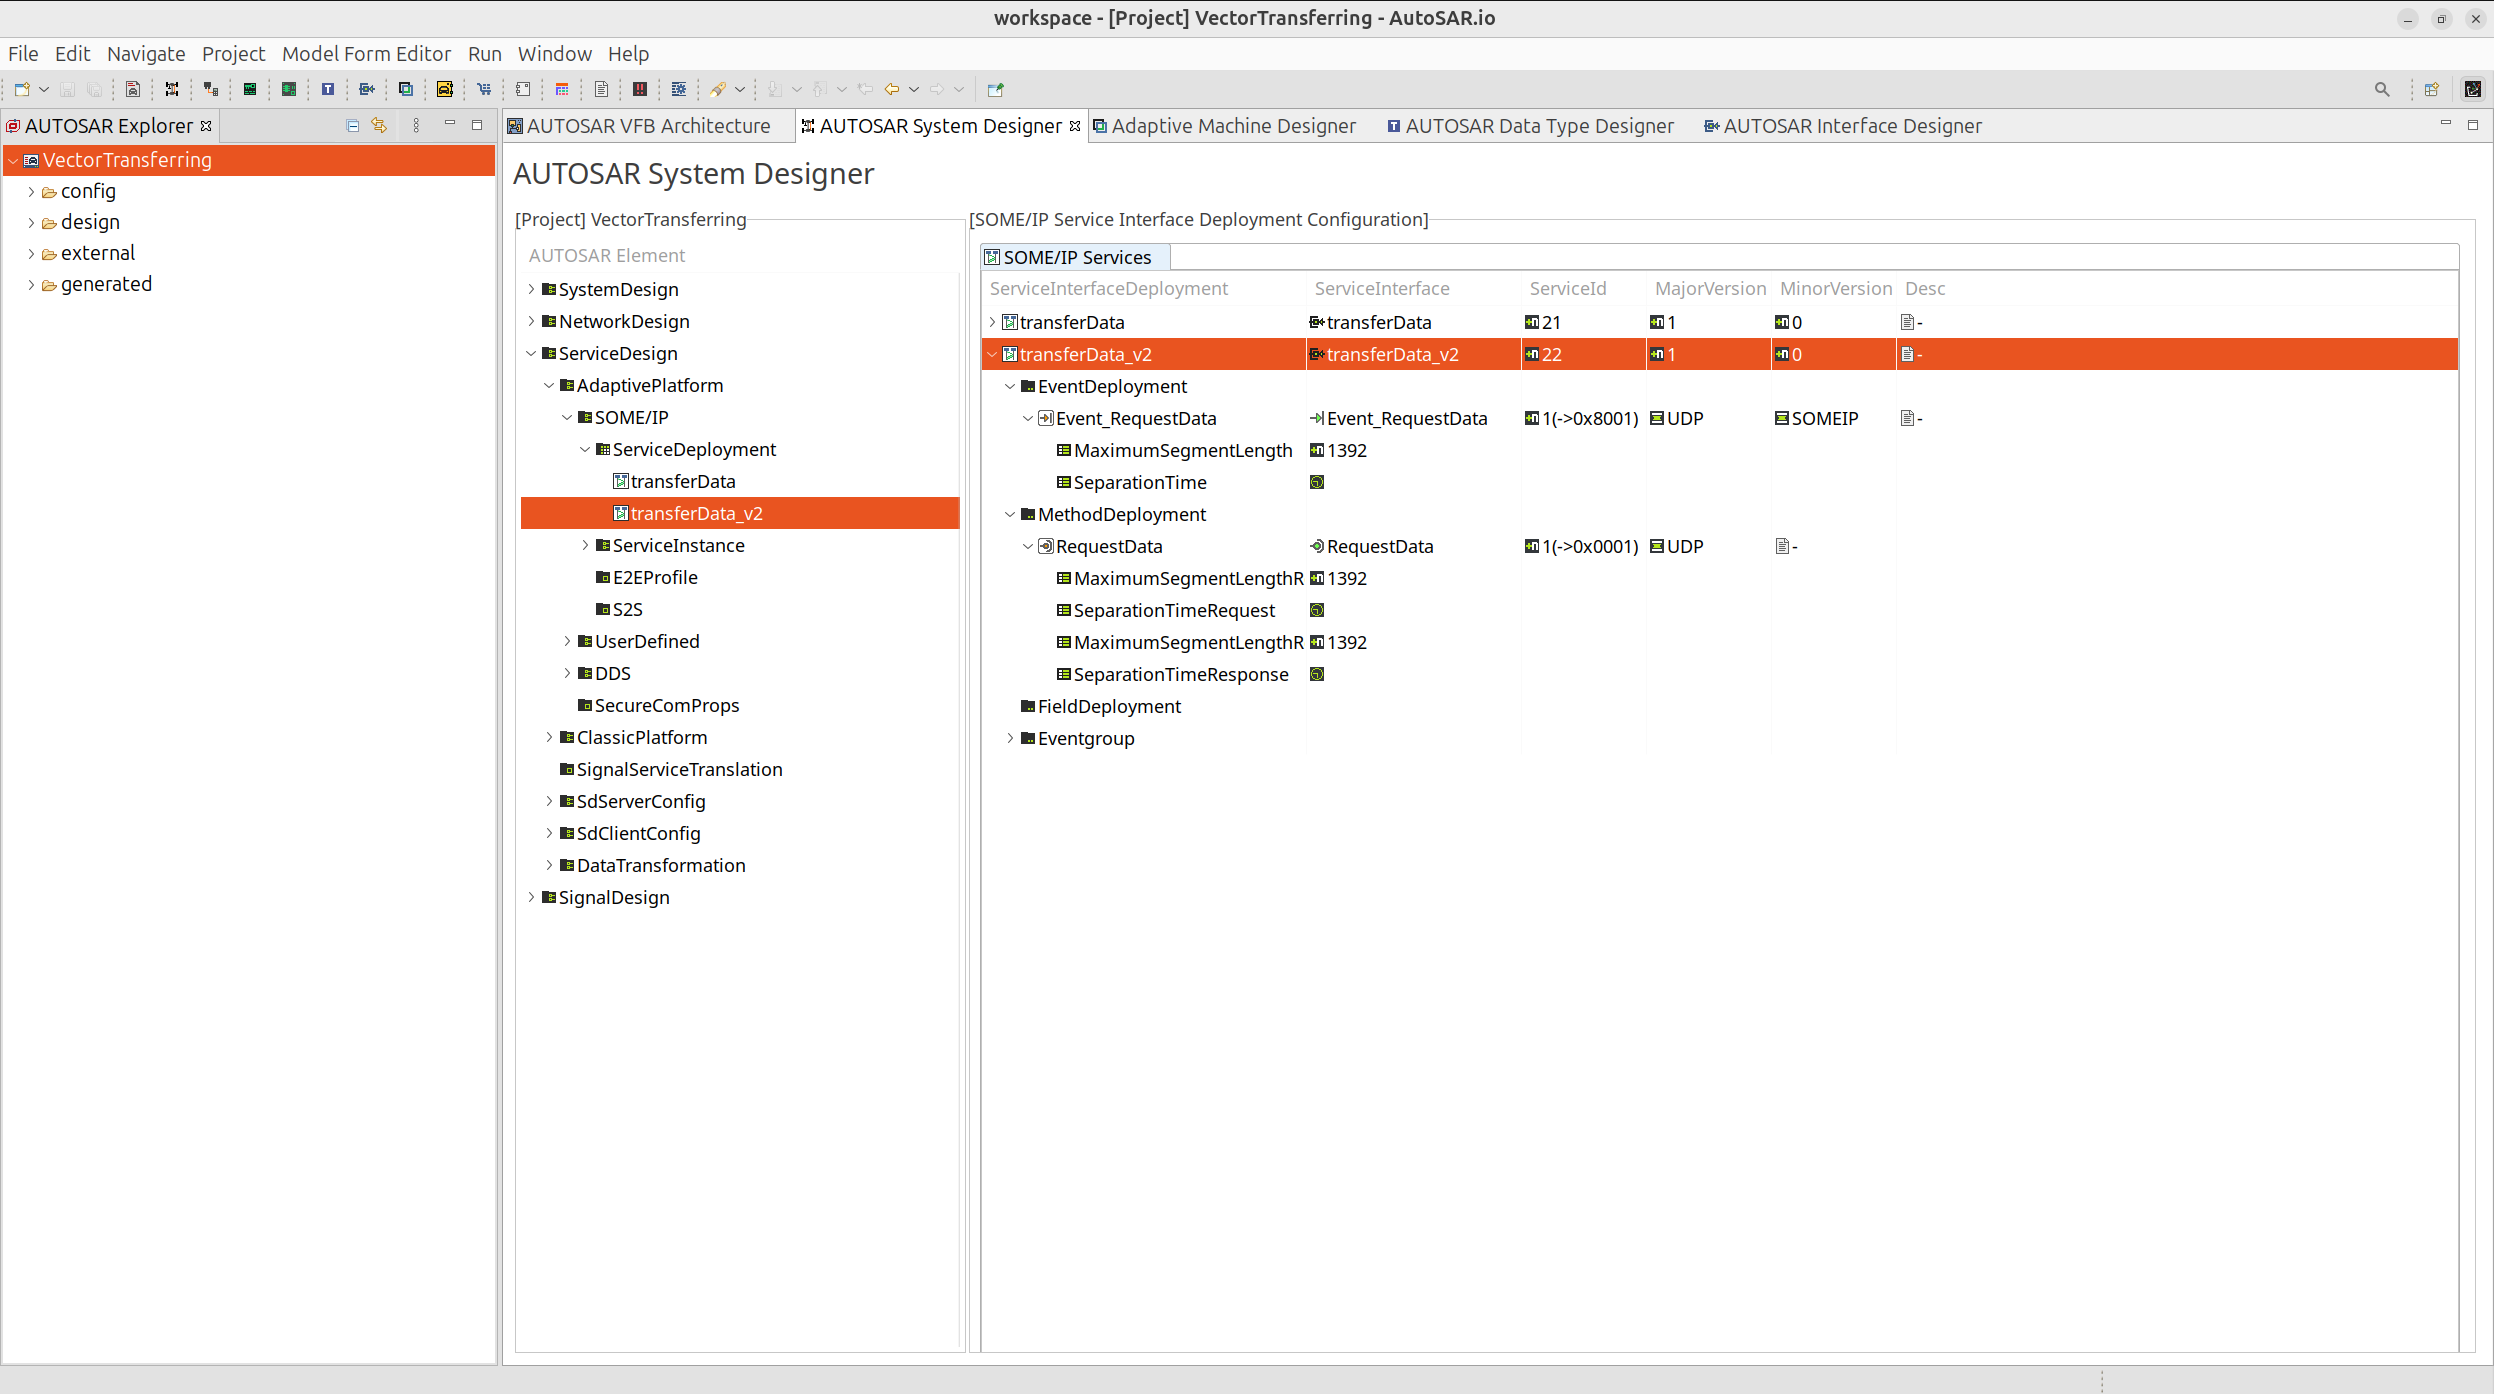
\includegraphics[width=0.75\textwidth]{Images/chap3/image_methodology/serviceInterfaceDesign/serviceDeployment.png}
    \vspace{0.5cm}
    \caption{Service Deployment Configuration}
    \label{fig:service_deployment}
\end{figure}

Figure~\ref{fig:service_deployment} illustrates the SOME/IP service deployment configuration for the \texttt{transferData\_v2} interface within the AUTOSAR System Designer. In this project, the service is explicitly deployed over SOME/IP with transport protocol (SOME/IP-TP) to support the transmission of large data payloads, such as image frames, between the ProviderSensor and ClientSensor applications.

The service is assigned a unique service identifier and version number and includes both event-based and method-based communication. The event \texttt{Event\_RequestData} is configured to use UDP transport together with a specified \texttt{MaximumSegmentLength}. This parameter plays a critical role in enabling SOME/IP-TP, as it informs the Adaptive AUTOSAR middleware that the transmitted data may exceed the maximum payload size of a single UDP packet and therefore must be segmented and reassembled at the receiver side.

Without configuring the \texttt{MaximumSegmentLength}, the communication would default to standard SOME/IP over UDP, which is suitable only for small messages and is not appropriate for transmitting image data. By explicitly defining this parameter, the deployment ensures that image payloads generated by the ProviderSensor are correctly fragmented, transmitted, and reassembled by the ClientSensor.

In addition to the event deployment, the \texttt{RequestData} method deployment specifies request and response timing parameters, supporting controlled client–server interaction when on-demand data transfer is required. Together, these configurations ensure that the \texttt{transferData\_v2} service can be reliably discovered via Service Discovery and can support both event-driven and request-based communication over SOME/IP-TP during runtime execution.


% Service instance provider configuration
\begin{figure}[H]
    \centering
    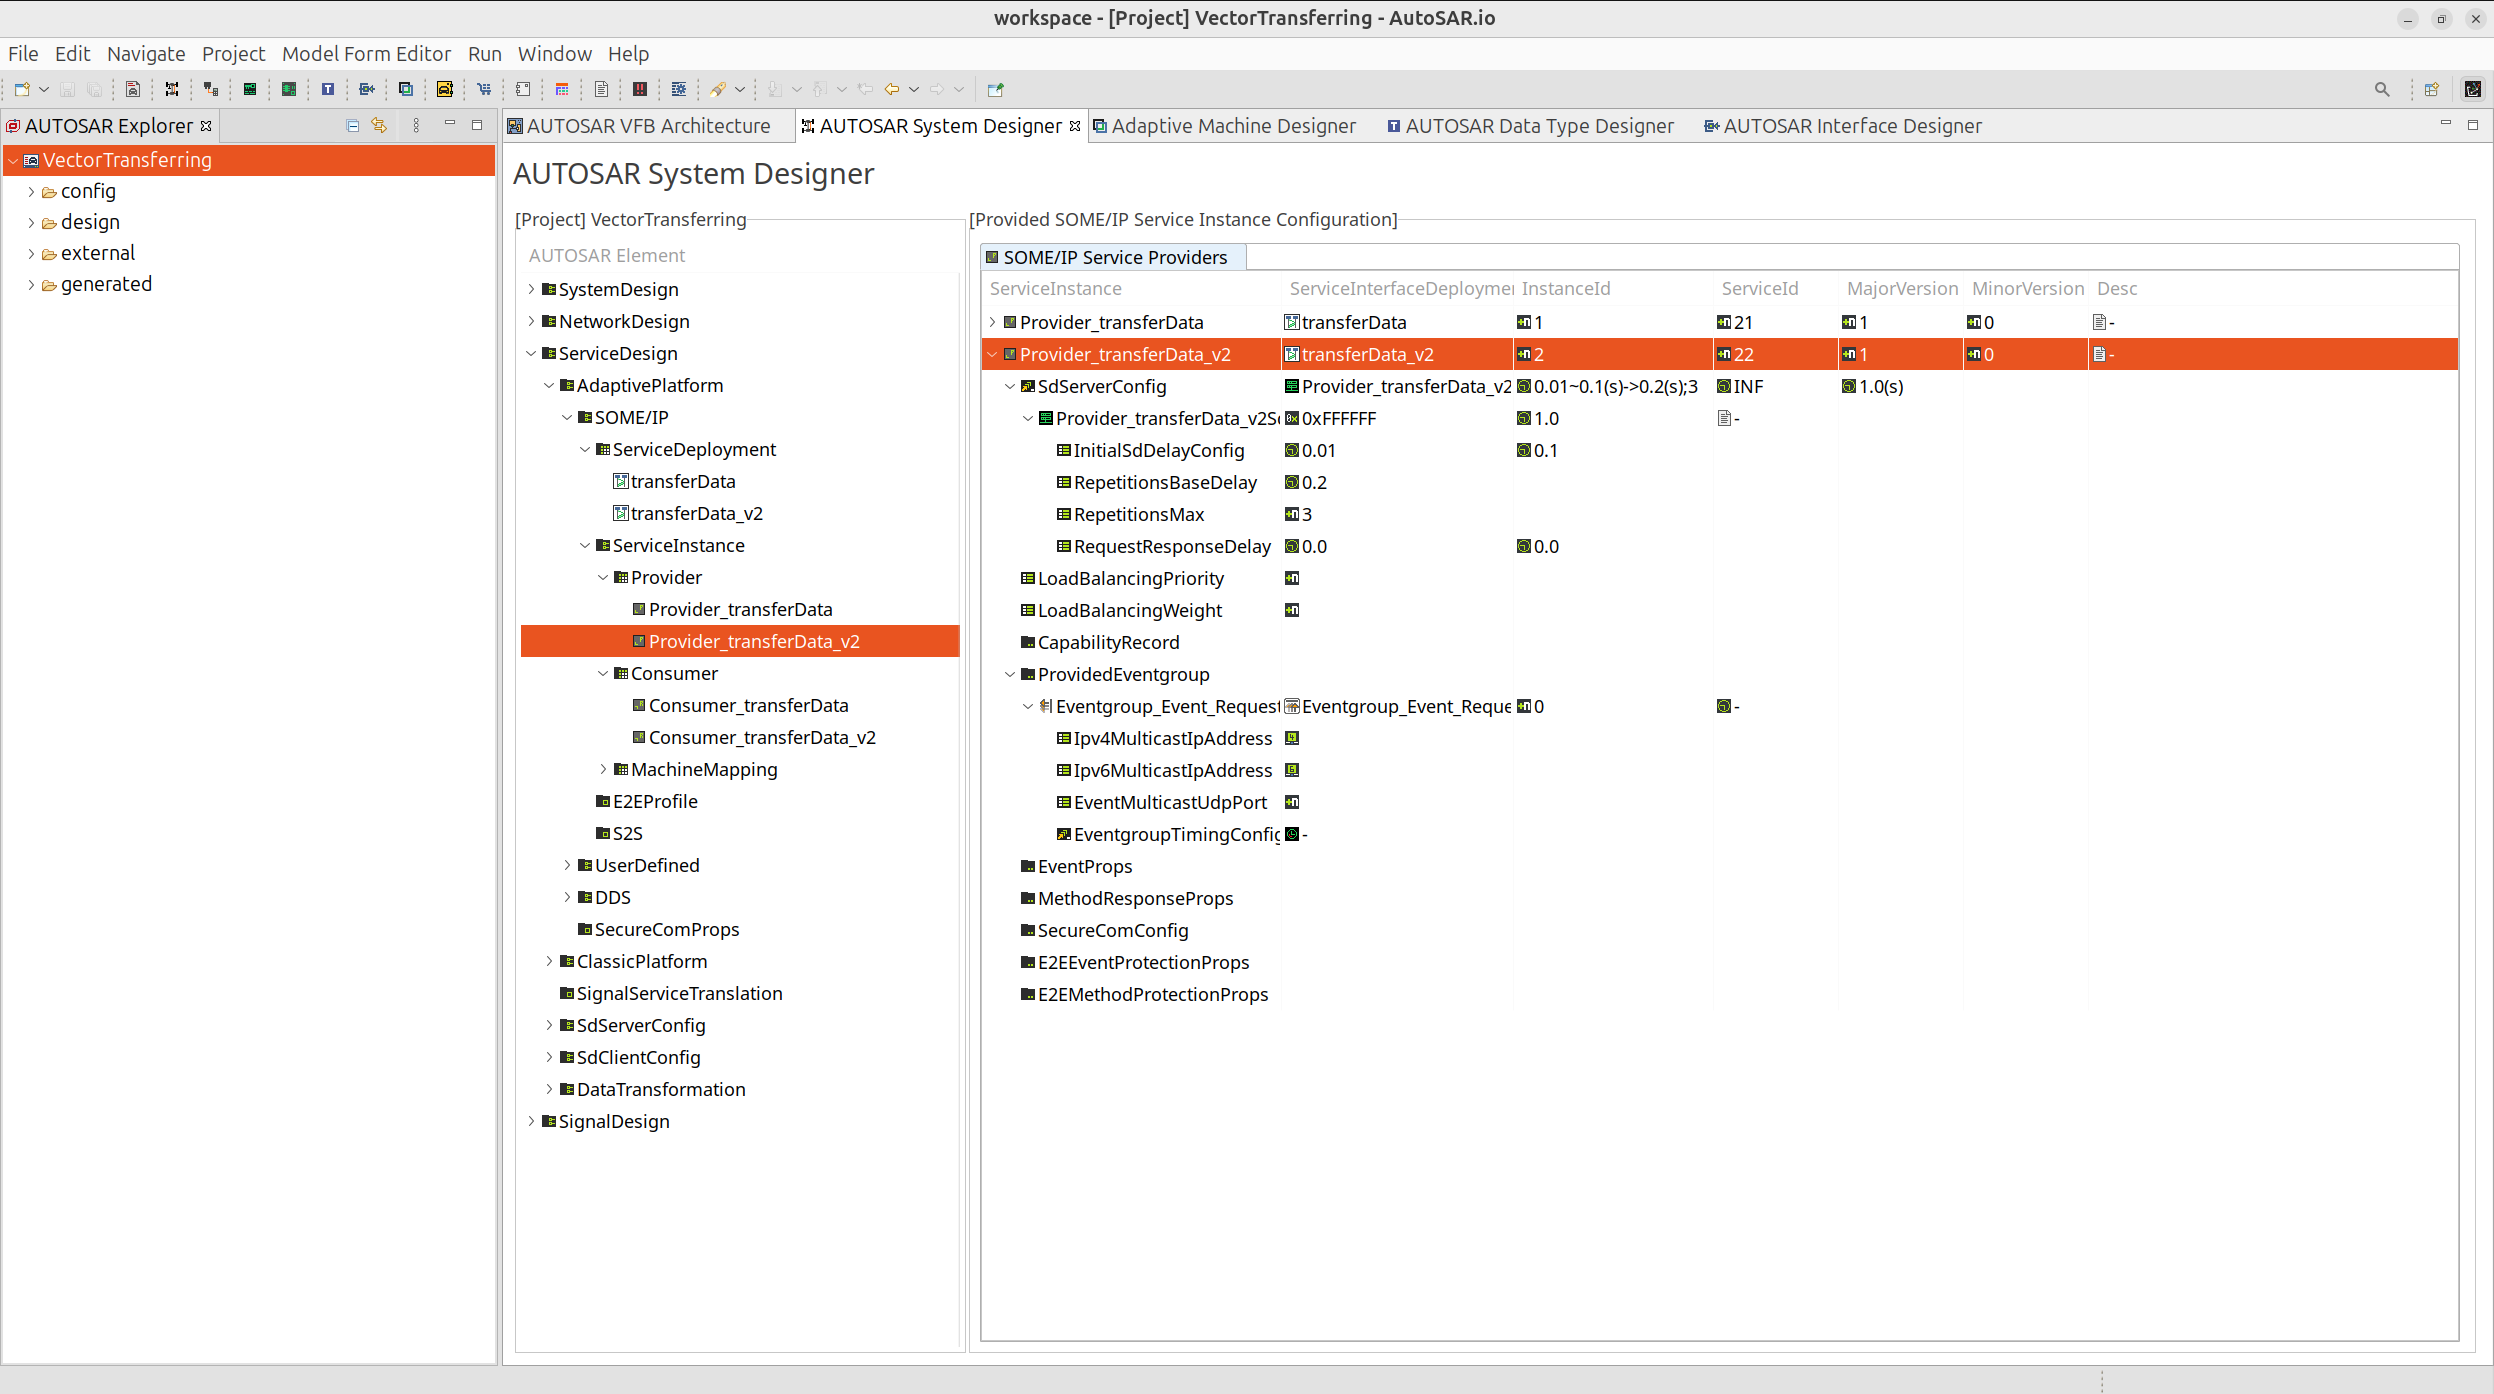
\includegraphics[width=0.75\textwidth]{Images/chap3/image_methodology/serviceInterfaceDesign/serviceInstance_Provider.png}
    \vspace{0.5cm}
    \caption{Service Instance Configuration for Provider}
    \label{fig:service_instance_provider}
\end{figure}

Figure~\ref{fig:service_instance_provider} illustrates the configuration of the SOME/IP service provider for the \texttt{transferData\_v2} interface. The provider instance is bound to a specific service and instance identifier with a defined major and minor version, ensuring compatibility with consuming applications. Server side parameters such as initial service offer delay, repetition base delay, and maximum repetitions are configured to control service availability announcements via Service Discovery. In addition, the provider defines event group settings for data notifications, together with timing and response related properties, which enable reliable dissemination of event based data to subscribed consumers during runtime.

% Service instance consumer configuration
\begin{figure}[H]
    \centering
    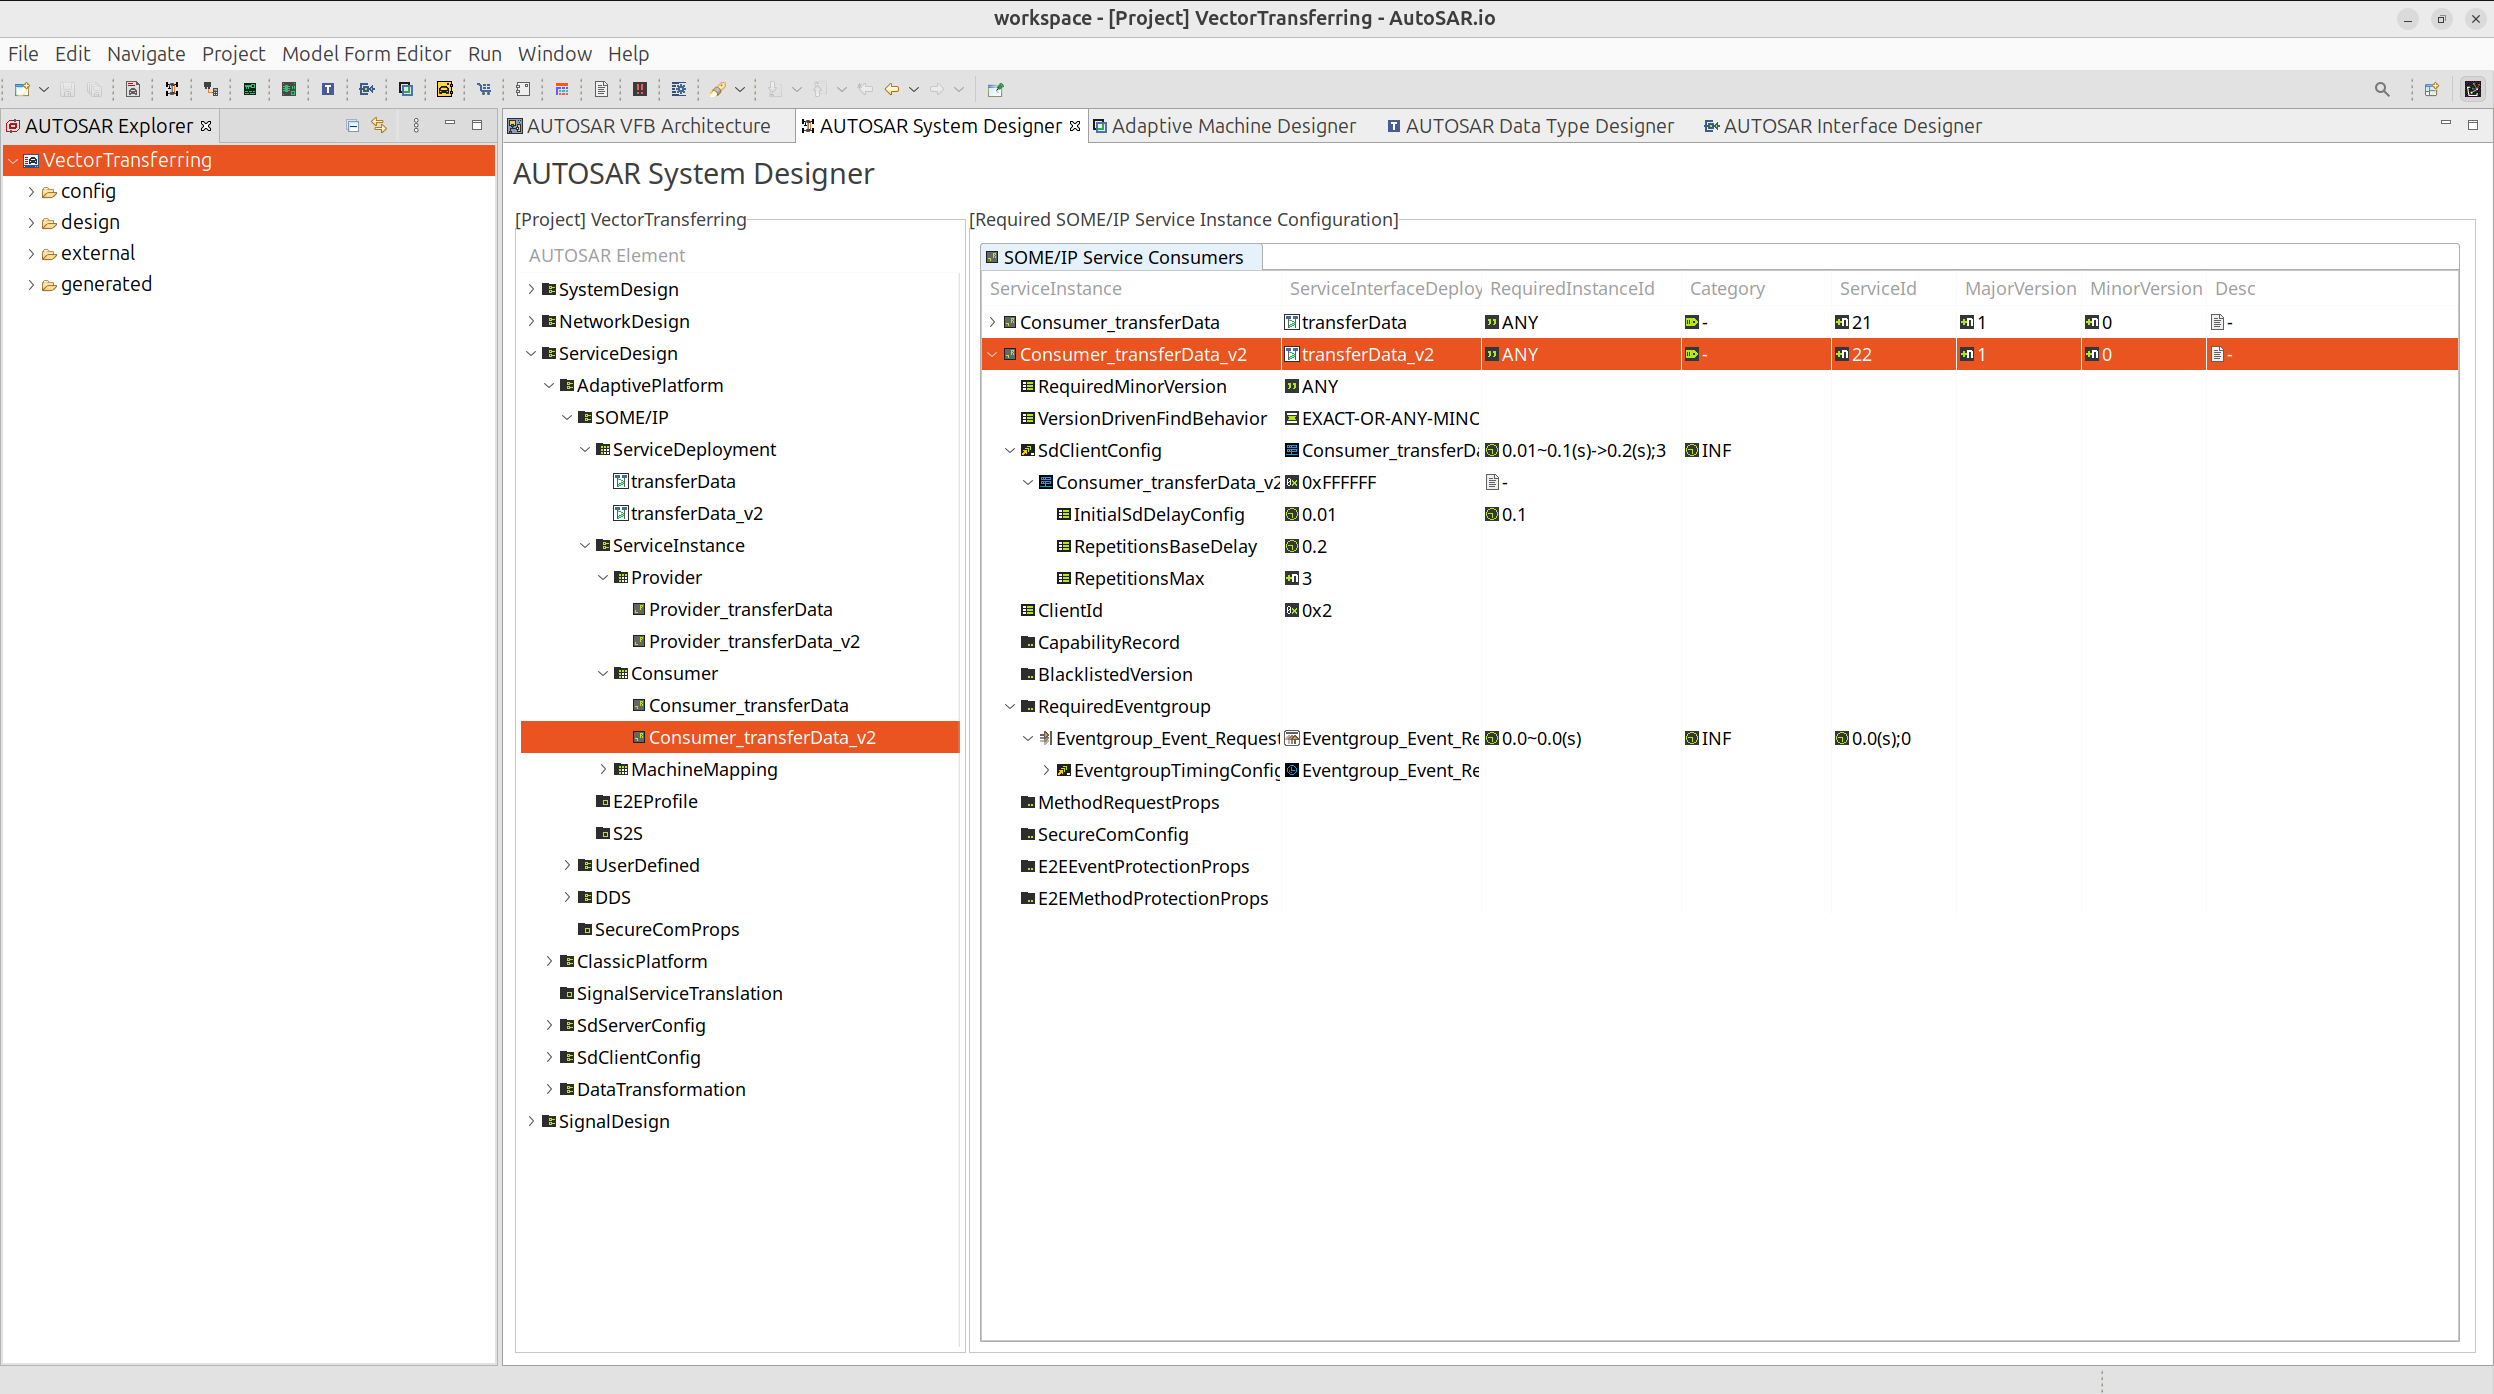
\includegraphics[width=0.75\textwidth]{Images/chap3/image_methodology/serviceInterfaceDesign/serviceInstance_Consumer.png}
    \vspace{0.5cm}
    \caption{Service Instance Configuration for Consumer}
    \label{fig:service_instance_consumer}
\end{figure}

Figure~\ref{fig:service_instance_consumer} presents the configuration of the corresponding SOME/IP service consumer acting as a subscriber to the \texttt{transferData\_v2} service. The consumer specifies flexible version requirements and discovery behavior, allowing it to bind to compatible provider instances at runtime. Client side parameters such as initial request delay, repetition strategy, and event group subscription settings determine how the consumer discovers the service and receives event notifications. Through this configuration, the consumer can dynamically subscribe to published data while maintaining controlled request and subscription behavior within the Adaptive AUTOSAR communication framework.

% Mapping service to machine network endpoint
\begin{figure}[H]
    \centering
    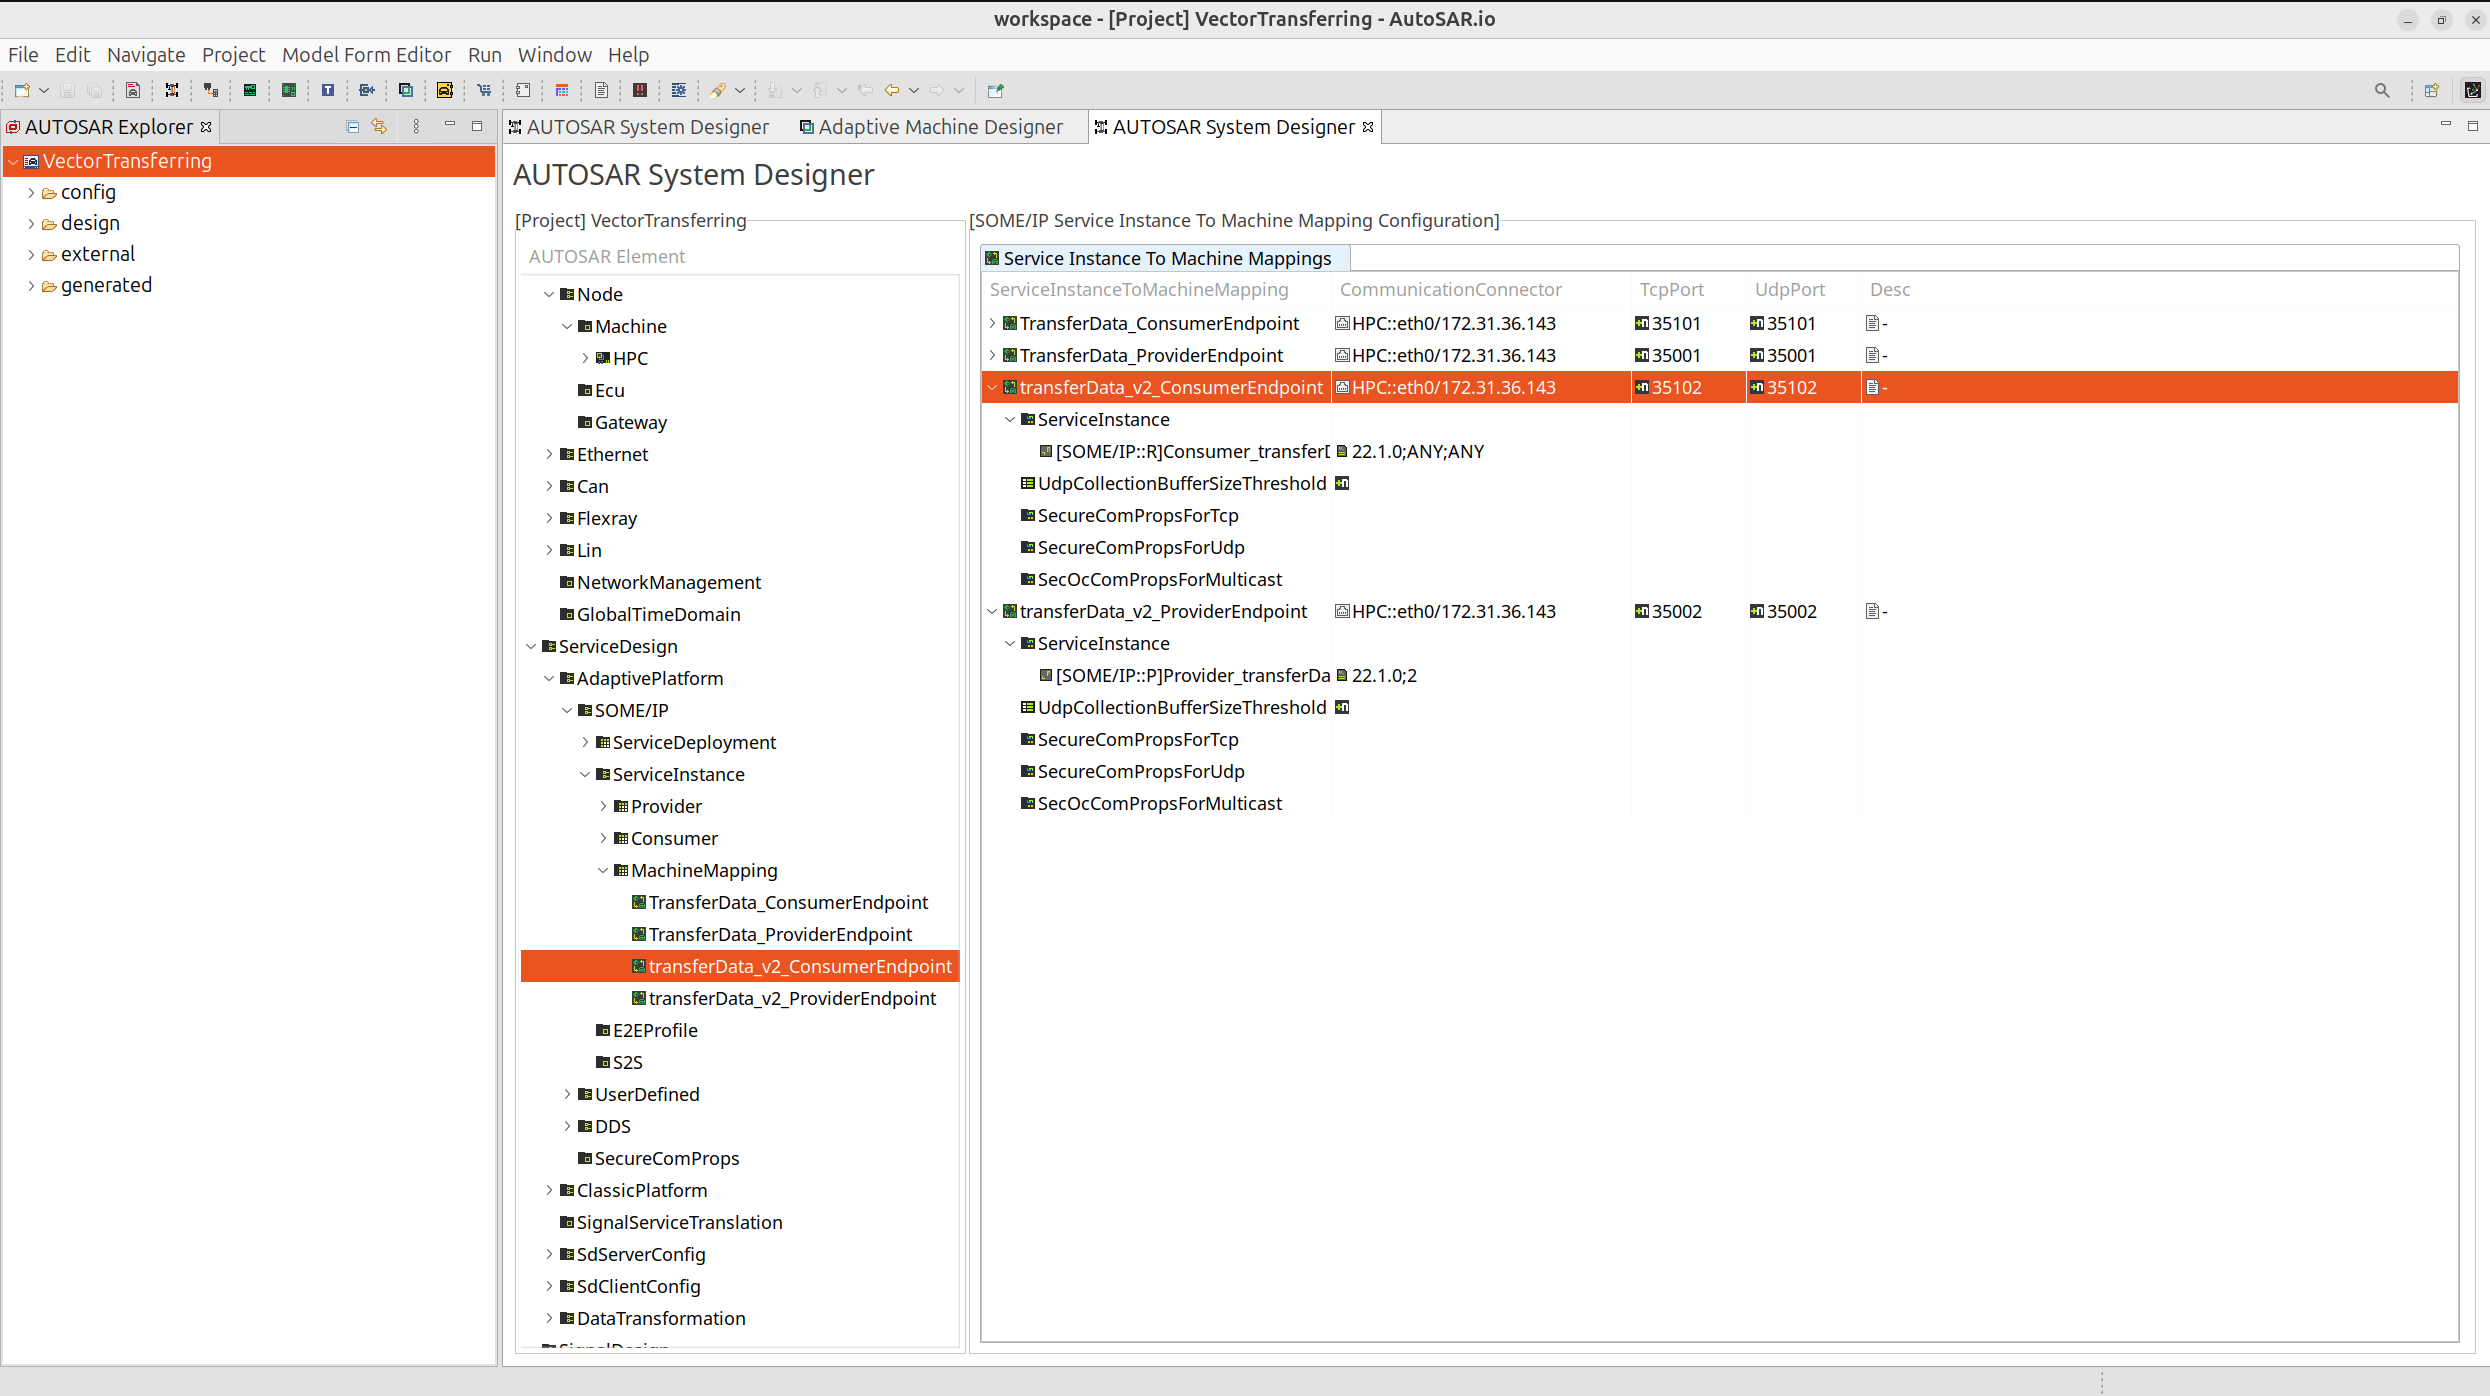
\includegraphics[width=0.75\textwidth]{Images/chap3/image_methodology/serviceInterfaceDesign/serviceMappingMachineEndpoint.png}
    \vspace{0.5cm}
    \caption{Mapping Service Instances to Machine Network Endpoint}
    \label{fig:service_machine_endpoint_mapping}
\end{figure}

Figure~\ref{fig:service_machine_endpoint_mapping} illustrates how the service instances of the \texttt{transferData} and \texttt{transferData\_v2} interfaces are bound to concrete machine network endpoints. Both provider and consumer instances are mapped to the Ethernet communication connector \texttt{HPC:eth0} with the fixed IPv4 address \texttt{172.31.36.143}, ensuring that all service communication is routed through a well defined network interface. Distinct TCP and UDP port numbers are assigned to each service instance, allowing concurrent data exchange while avoiding port conflicts.

This mapping explicitly links abstract service definitions to physical network resources, enabling correct runtime deployment and communication over SOME/IP. By defining separate endpoints for provider and consumer roles, the configuration supports clear role separation and reliable message routing between applications deployed on the same machine or across different nodes in the Adaptive AUTOSAR system.

\begin{figure}[H]
    \centering
    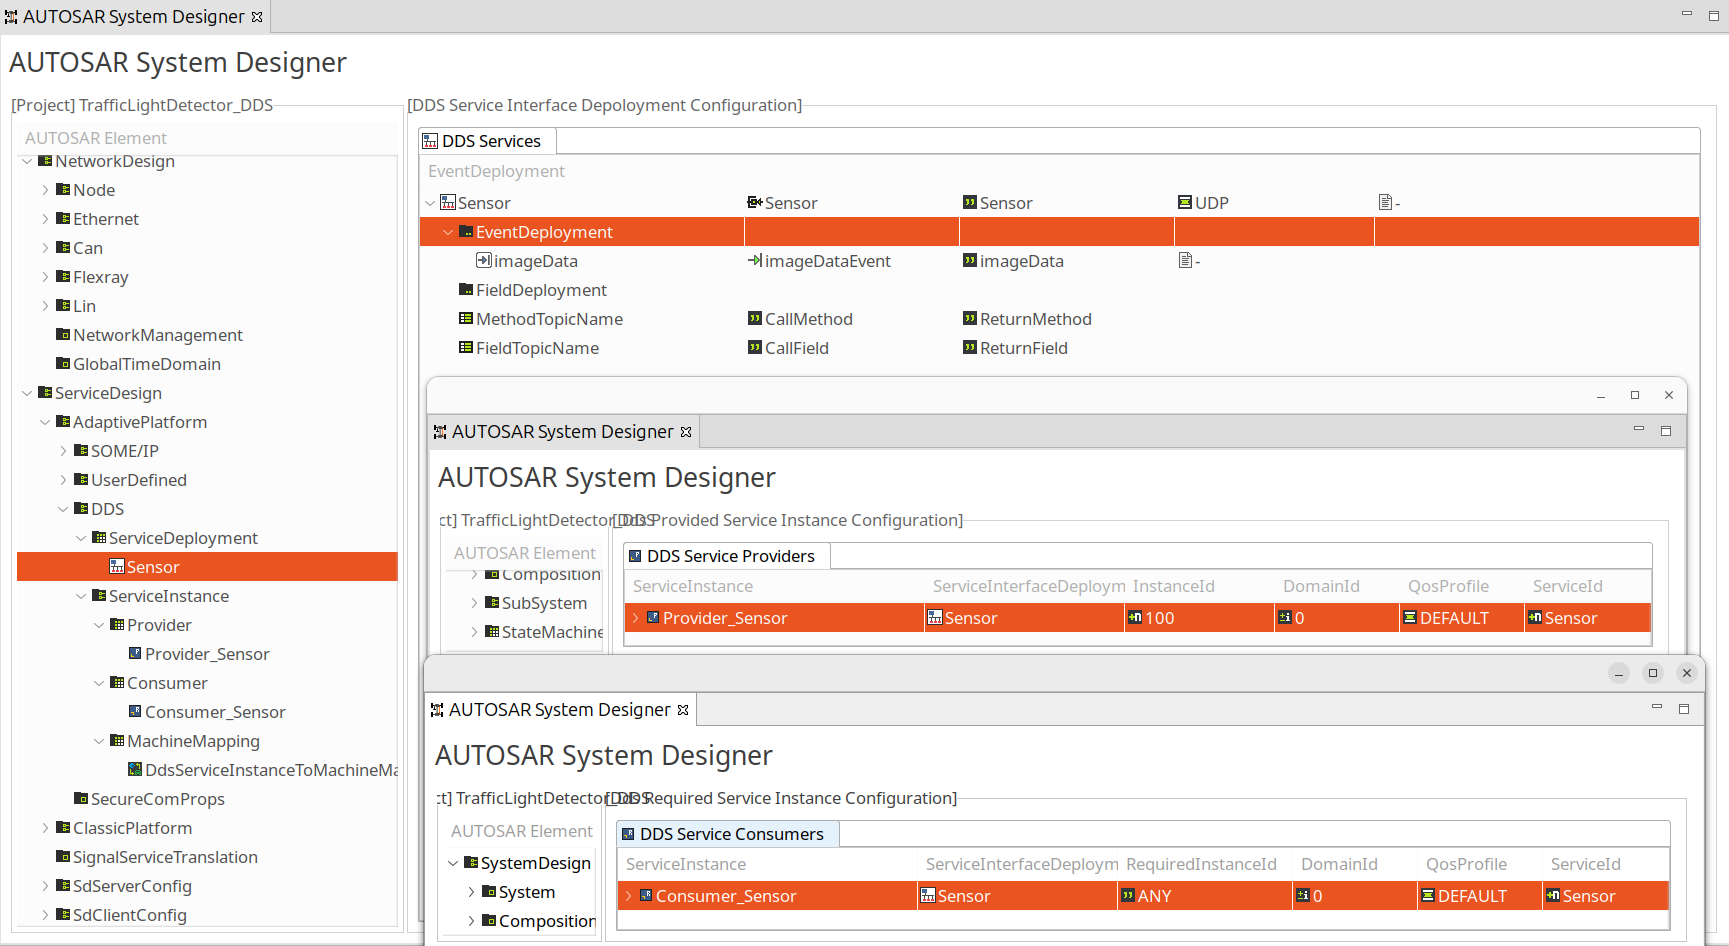
\includegraphics[width=0.75\textwidth]{Images/chap3/image_methodology/serviceInterfaceDesign/DDS_Config.png}
    \vspace{0.5cm}
    \caption{Mapping Service Instances to Machine Network Endpoint}
    \label{fig:dds_config}
\end{figure}

Similarly to the SOME/IP configuration, Figure~\ref{fig:dds_config} presents the DDS-based deployment configuration used for the \texttt{Sensor} service. In the DDS Service Interface Deployment Configuration, the service interface is deployed with the \texttt{imageDataEvent} event and the corresponding DDS topic \texttt{imageData}. The event deployment is configured to use UDP transport, allowing the Provider and Client applications to exchange image and metadata payloads through DDS publish/subscribe communication.

The provided service instance is configured as \texttt{Provider\_Sensor}, bound to the \texttt{Sensor} service deployment with instance-id~\texttt{100}, DDS Domain Id~\texttt{0}, and the \texttt{DEFAULT} QoS profile. The required service instance is configured as \texttt{Consumer\_Sensor}, also bound to the same \texttt{Sensor} service deployment, but with required instance-id~\texttt{ANY}. This configuration allows the Client application to discover and subscribe to the Provider service instance dynamically within the same DDS domain.

Through this DDS configuration, the abstract AUTOSAR service definition is mapped to concrete DDS communication entities, including service deployment, topic, event, provider instance, consumer instance, domain identifier, and QoS profile. This mapping is essential for the implemented prototype because the runtime communication between \texttt{ProviderSensor} and \texttt{ClientSensor} is realized through DDS rather than SOME/IP. As a result, the system can publish \texttt{imageDataEvent} samples on the \texttt{imageData} topic and deliver the \texttt{GpsJpegWireHeader + JPEG} payload from the Provider to the Client in a service-oriented and configurable manner.

\subsubsection{Application Design}

% Modeling Adaptive Application
\begin{figure}[H]
    \centering
    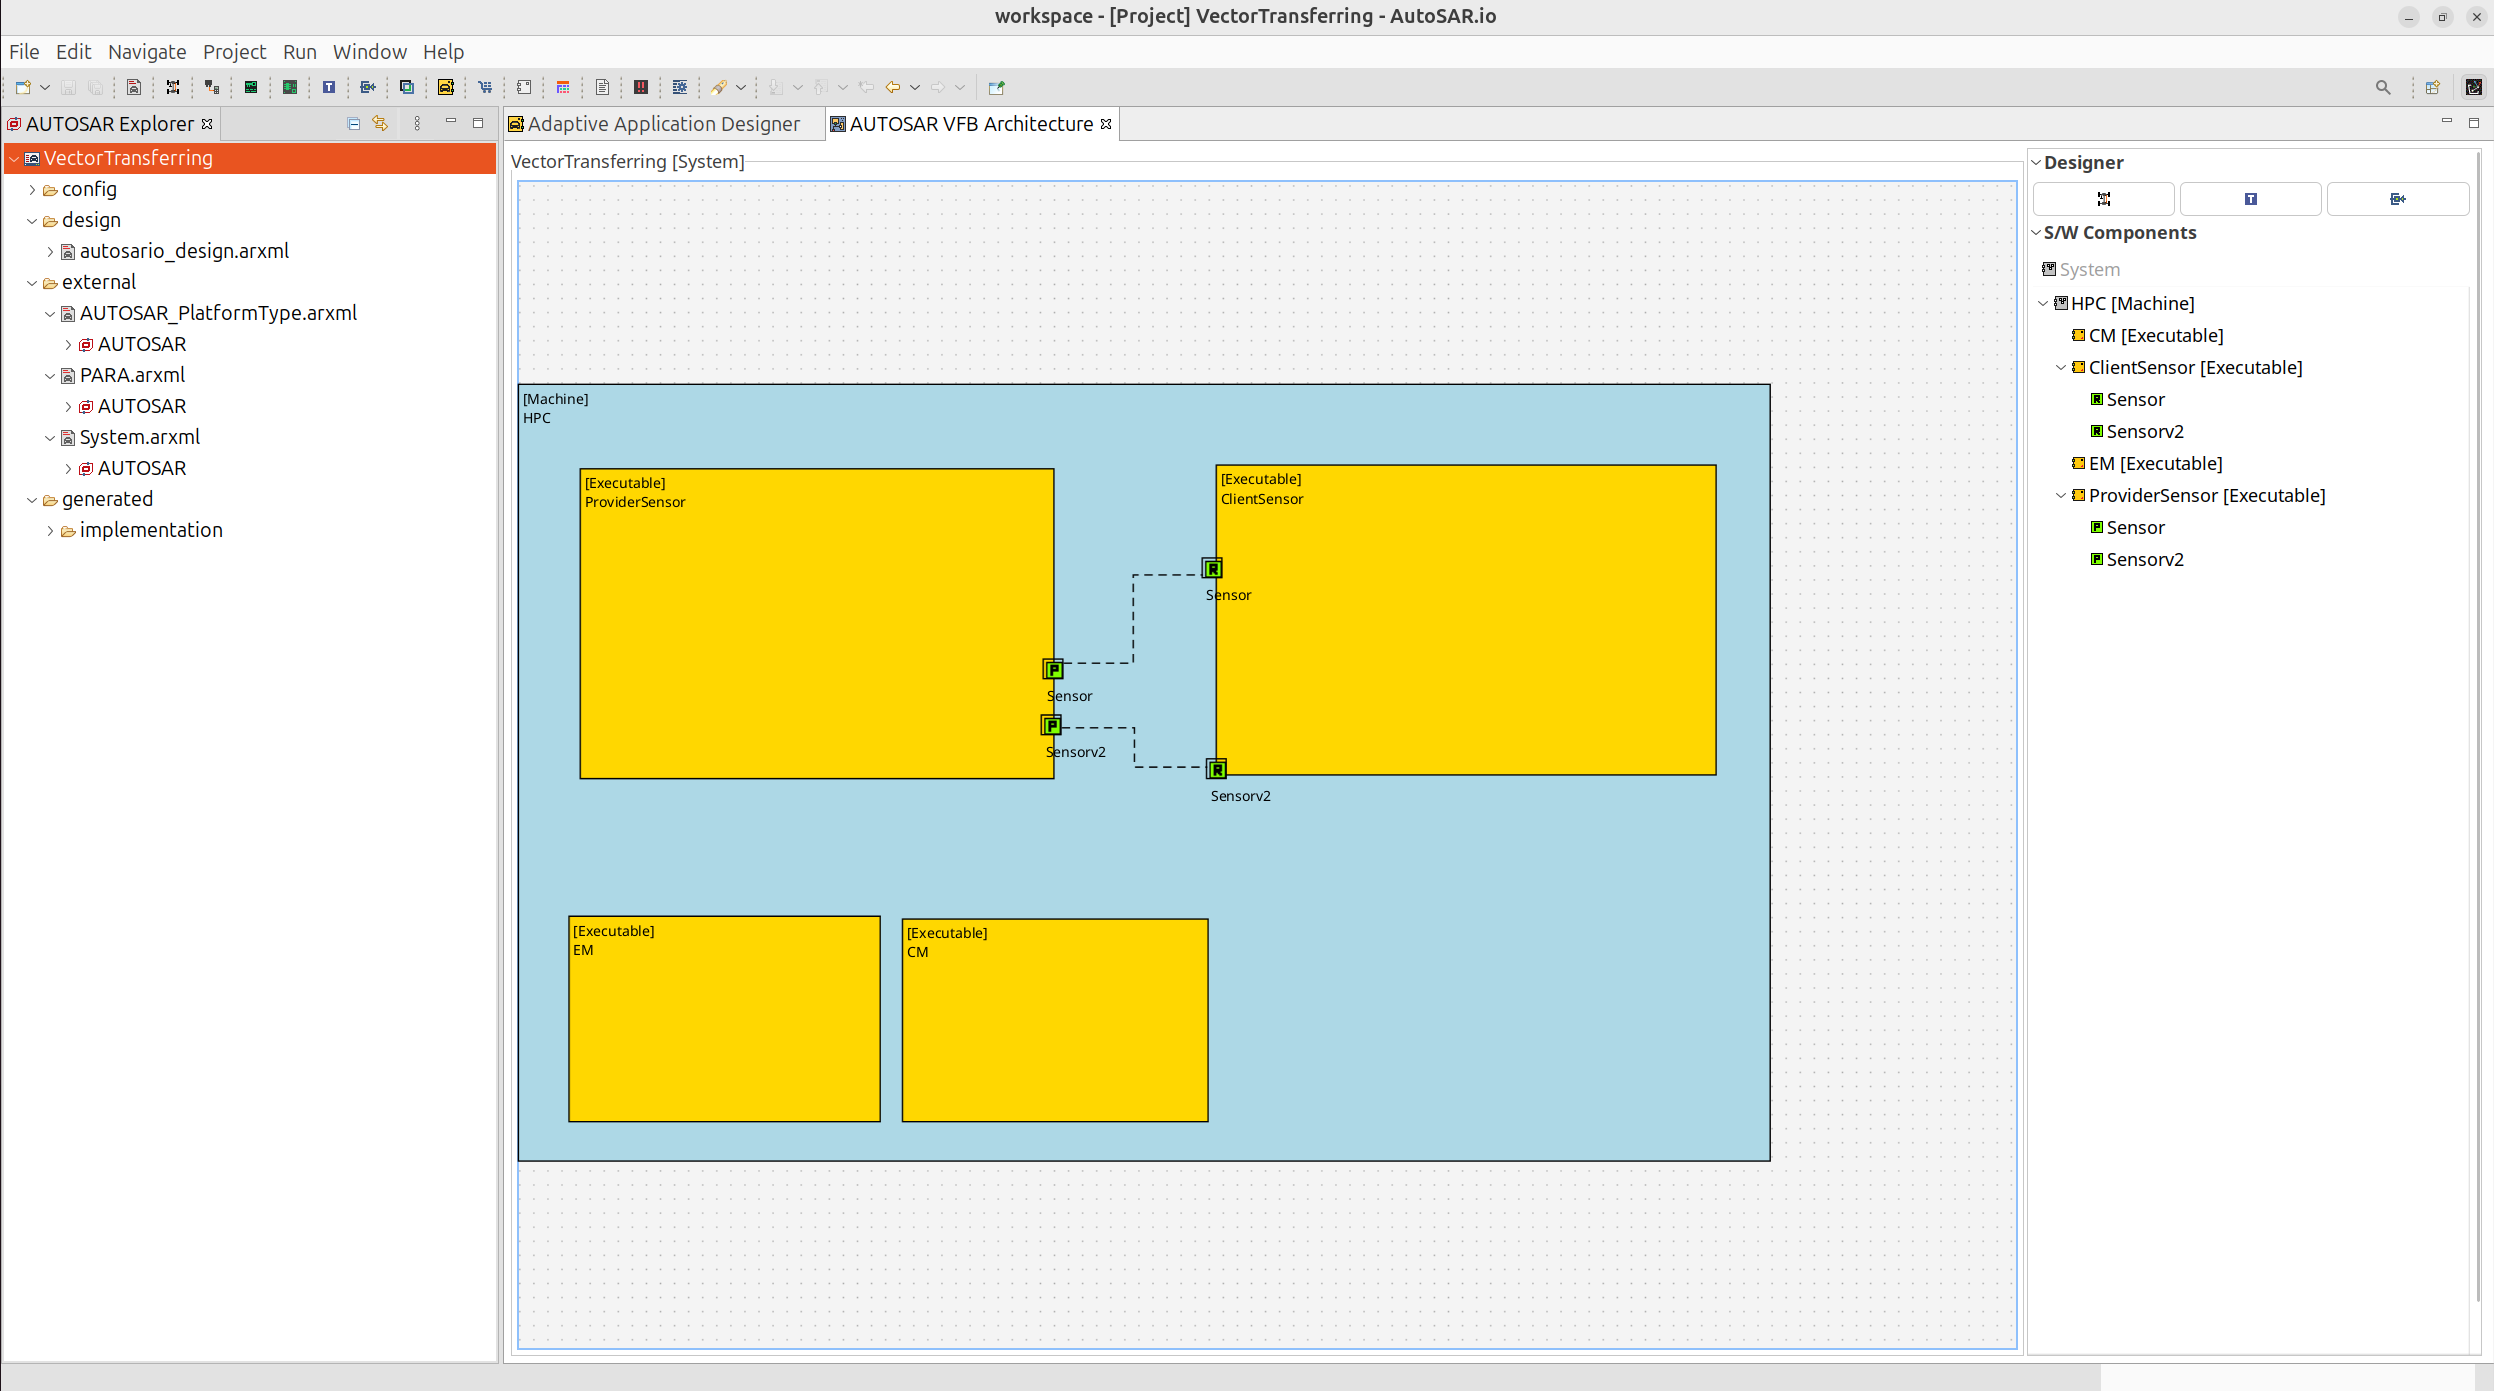
\includegraphics[width=0.75\textwidth]{Images/chap3/image_methodology/applicationDesign/modelingApplication.png}
    \vspace{0.5cm}
    \caption{Modeling of Adaptive Application}
    \label{fig:modeling_application}
\end{figure}

Figure~\ref{fig:modeling_application} shows the Adaptive Application modeling view, where users define the overall application architecture by assigning application executables to a specific machine. In this workspace, the target machine \texttt{HPC} is selected as the deployment context, and multiple executables such as \texttt{ProviderSensor}, \texttt{ClientSensor}, \texttt{CM}, and \texttt{EM} are instantiated within it. Logical connections between executables are visually represented through ports, allowing designers to describe interaction relationships at the architectural level. This model serves as a central design step that links application executables with the underlying machine, providing a clear and structured representation of how software components are organized and deployed in an Adaptive AUTOSAR system.


% Configure Provider Executable Properties
\begin{figure}[H]
    \centering
    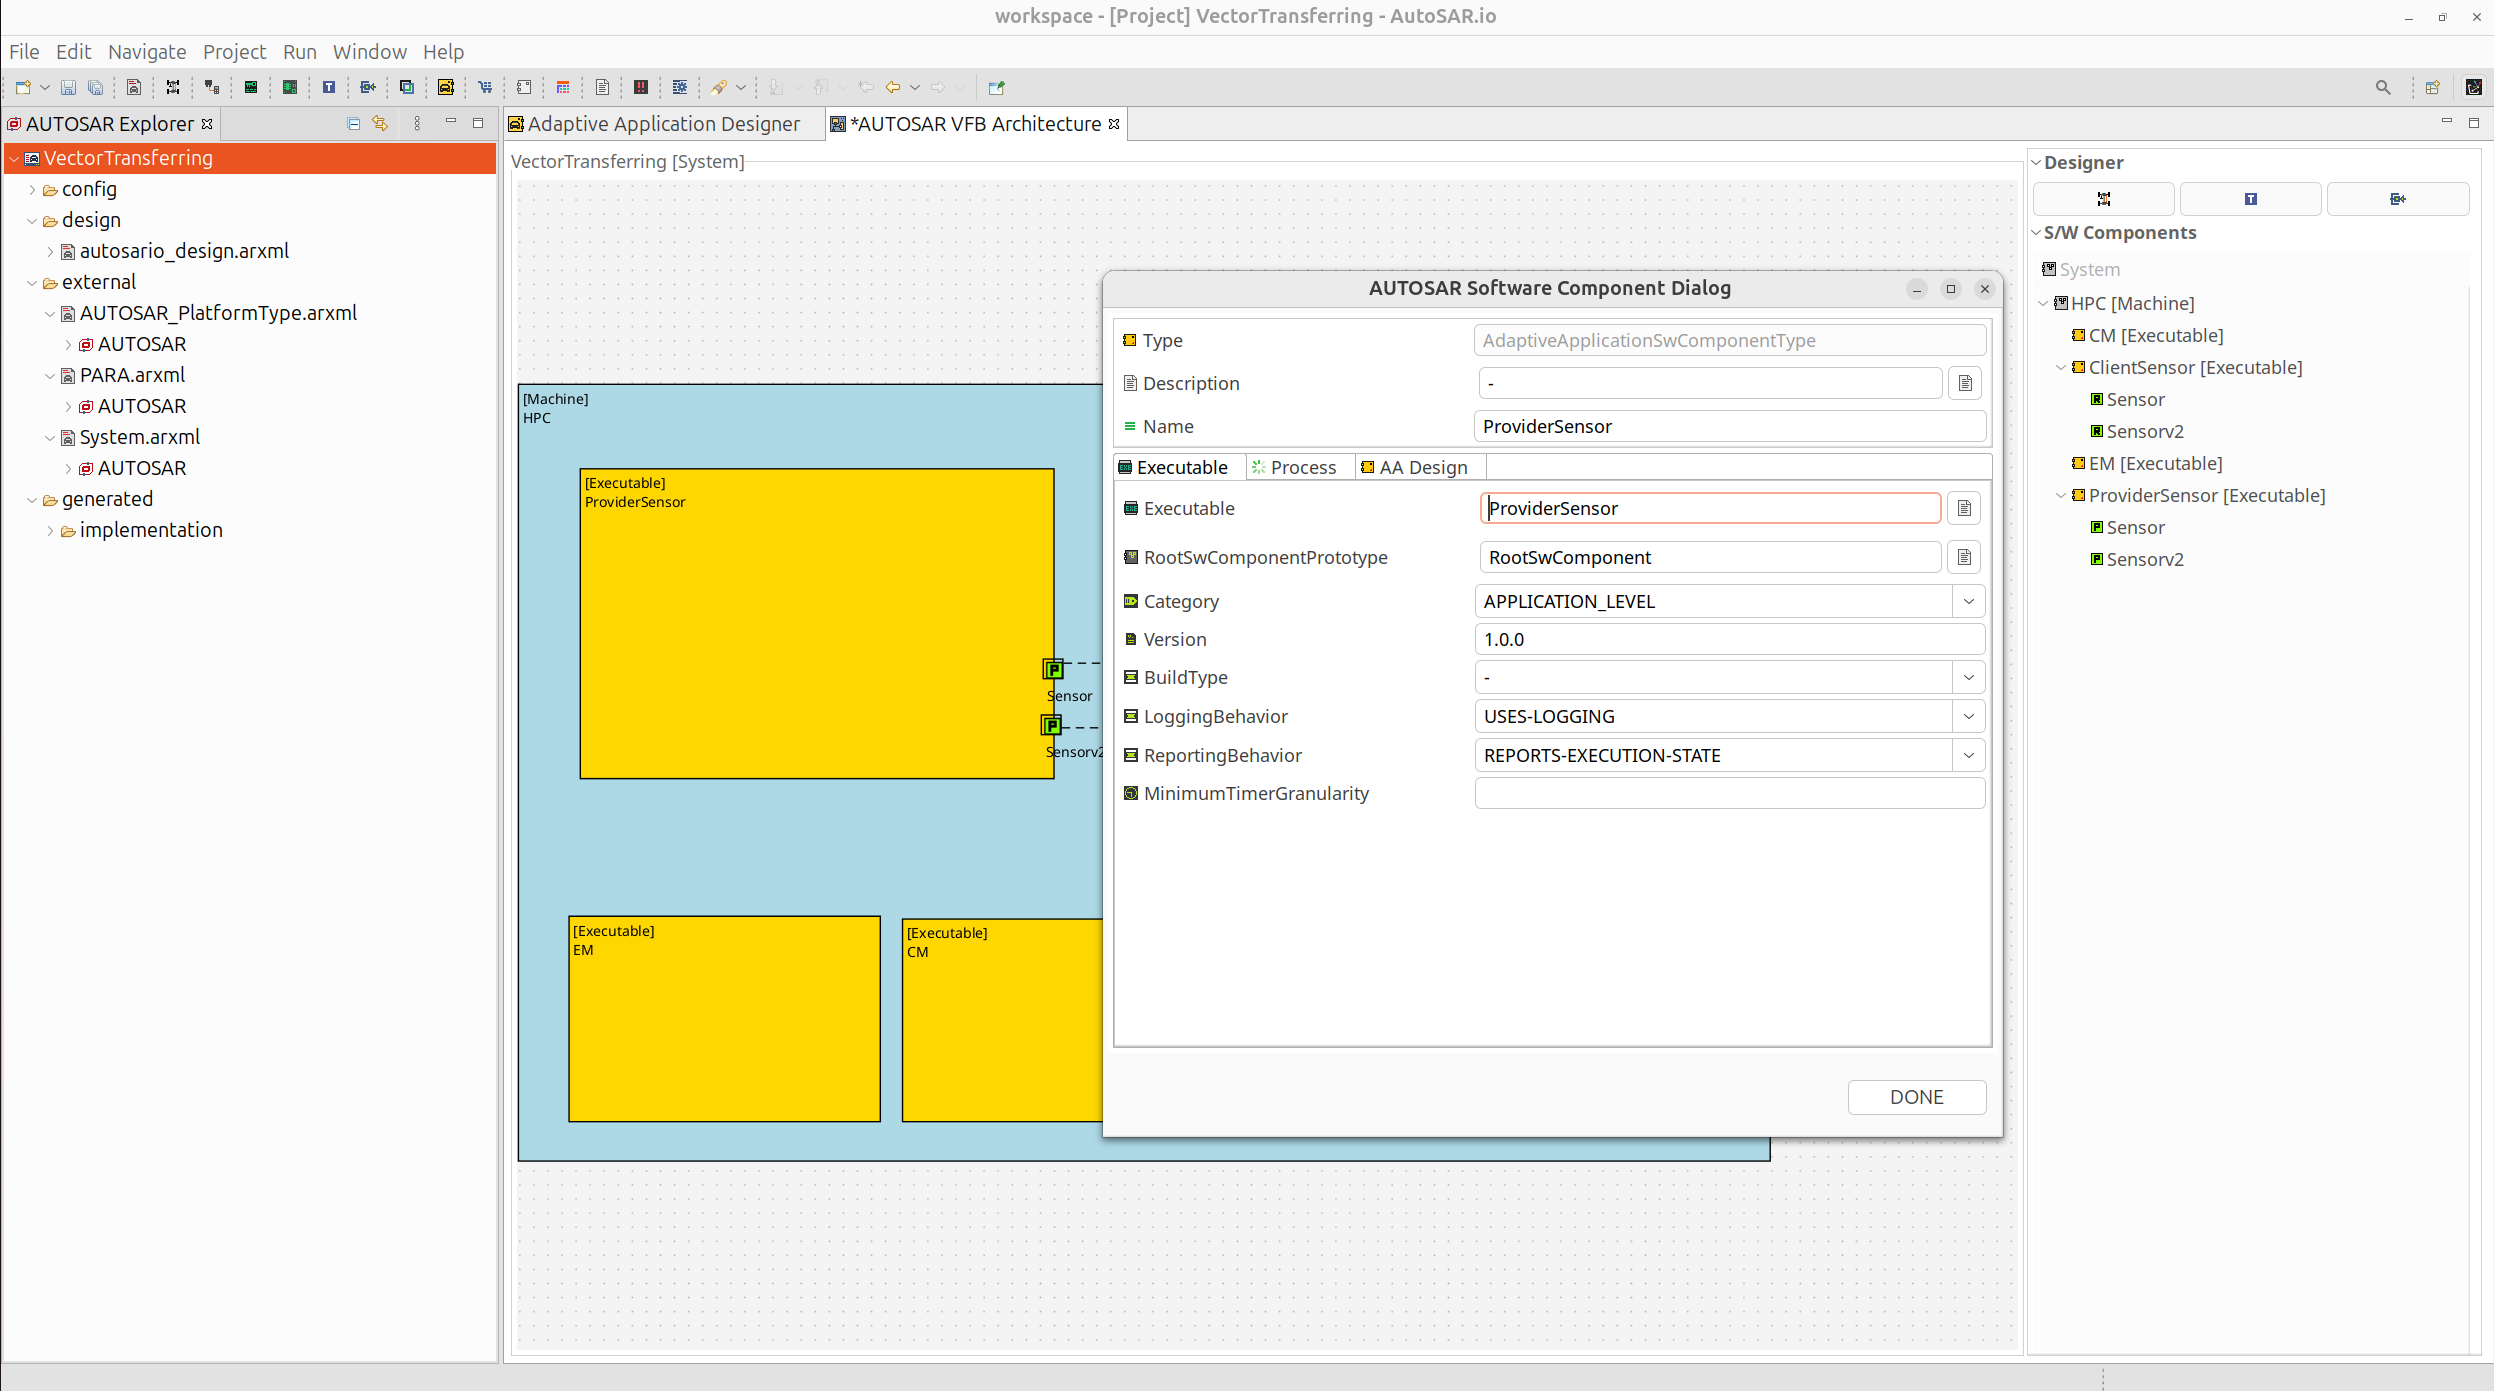
\includegraphics[width=0.75\textwidth]{Images/chap3/image_methodology/applicationDesign/providerExProperties.png}
    \vspace{0.5cm}
    \caption{Configuration of Provider Executable Properties}
    \label{fig:app_provider_executable_properties}
\end{figure}

Figure~\ref{fig:app_provider_executable_properties} presents the configuration of the provider application executable within the Adaptive Application Designer. In this view, the executable \texttt{ProviderSensor} is defined as an application level software component with a specific version and logging behavior. Key properties such as execution category, reporting behavior, and minimum timer granularity are configured to control runtime characteristics and observability. By assigning these attributes, the provider executable is clearly identified as a service offering entity and is prepared to integrate with the Adaptive AUTOSAR execution environment in a consistent and manageable manner.

% Map Provider Ports to Service Interface
\begin{figure}[H]
    \centering
    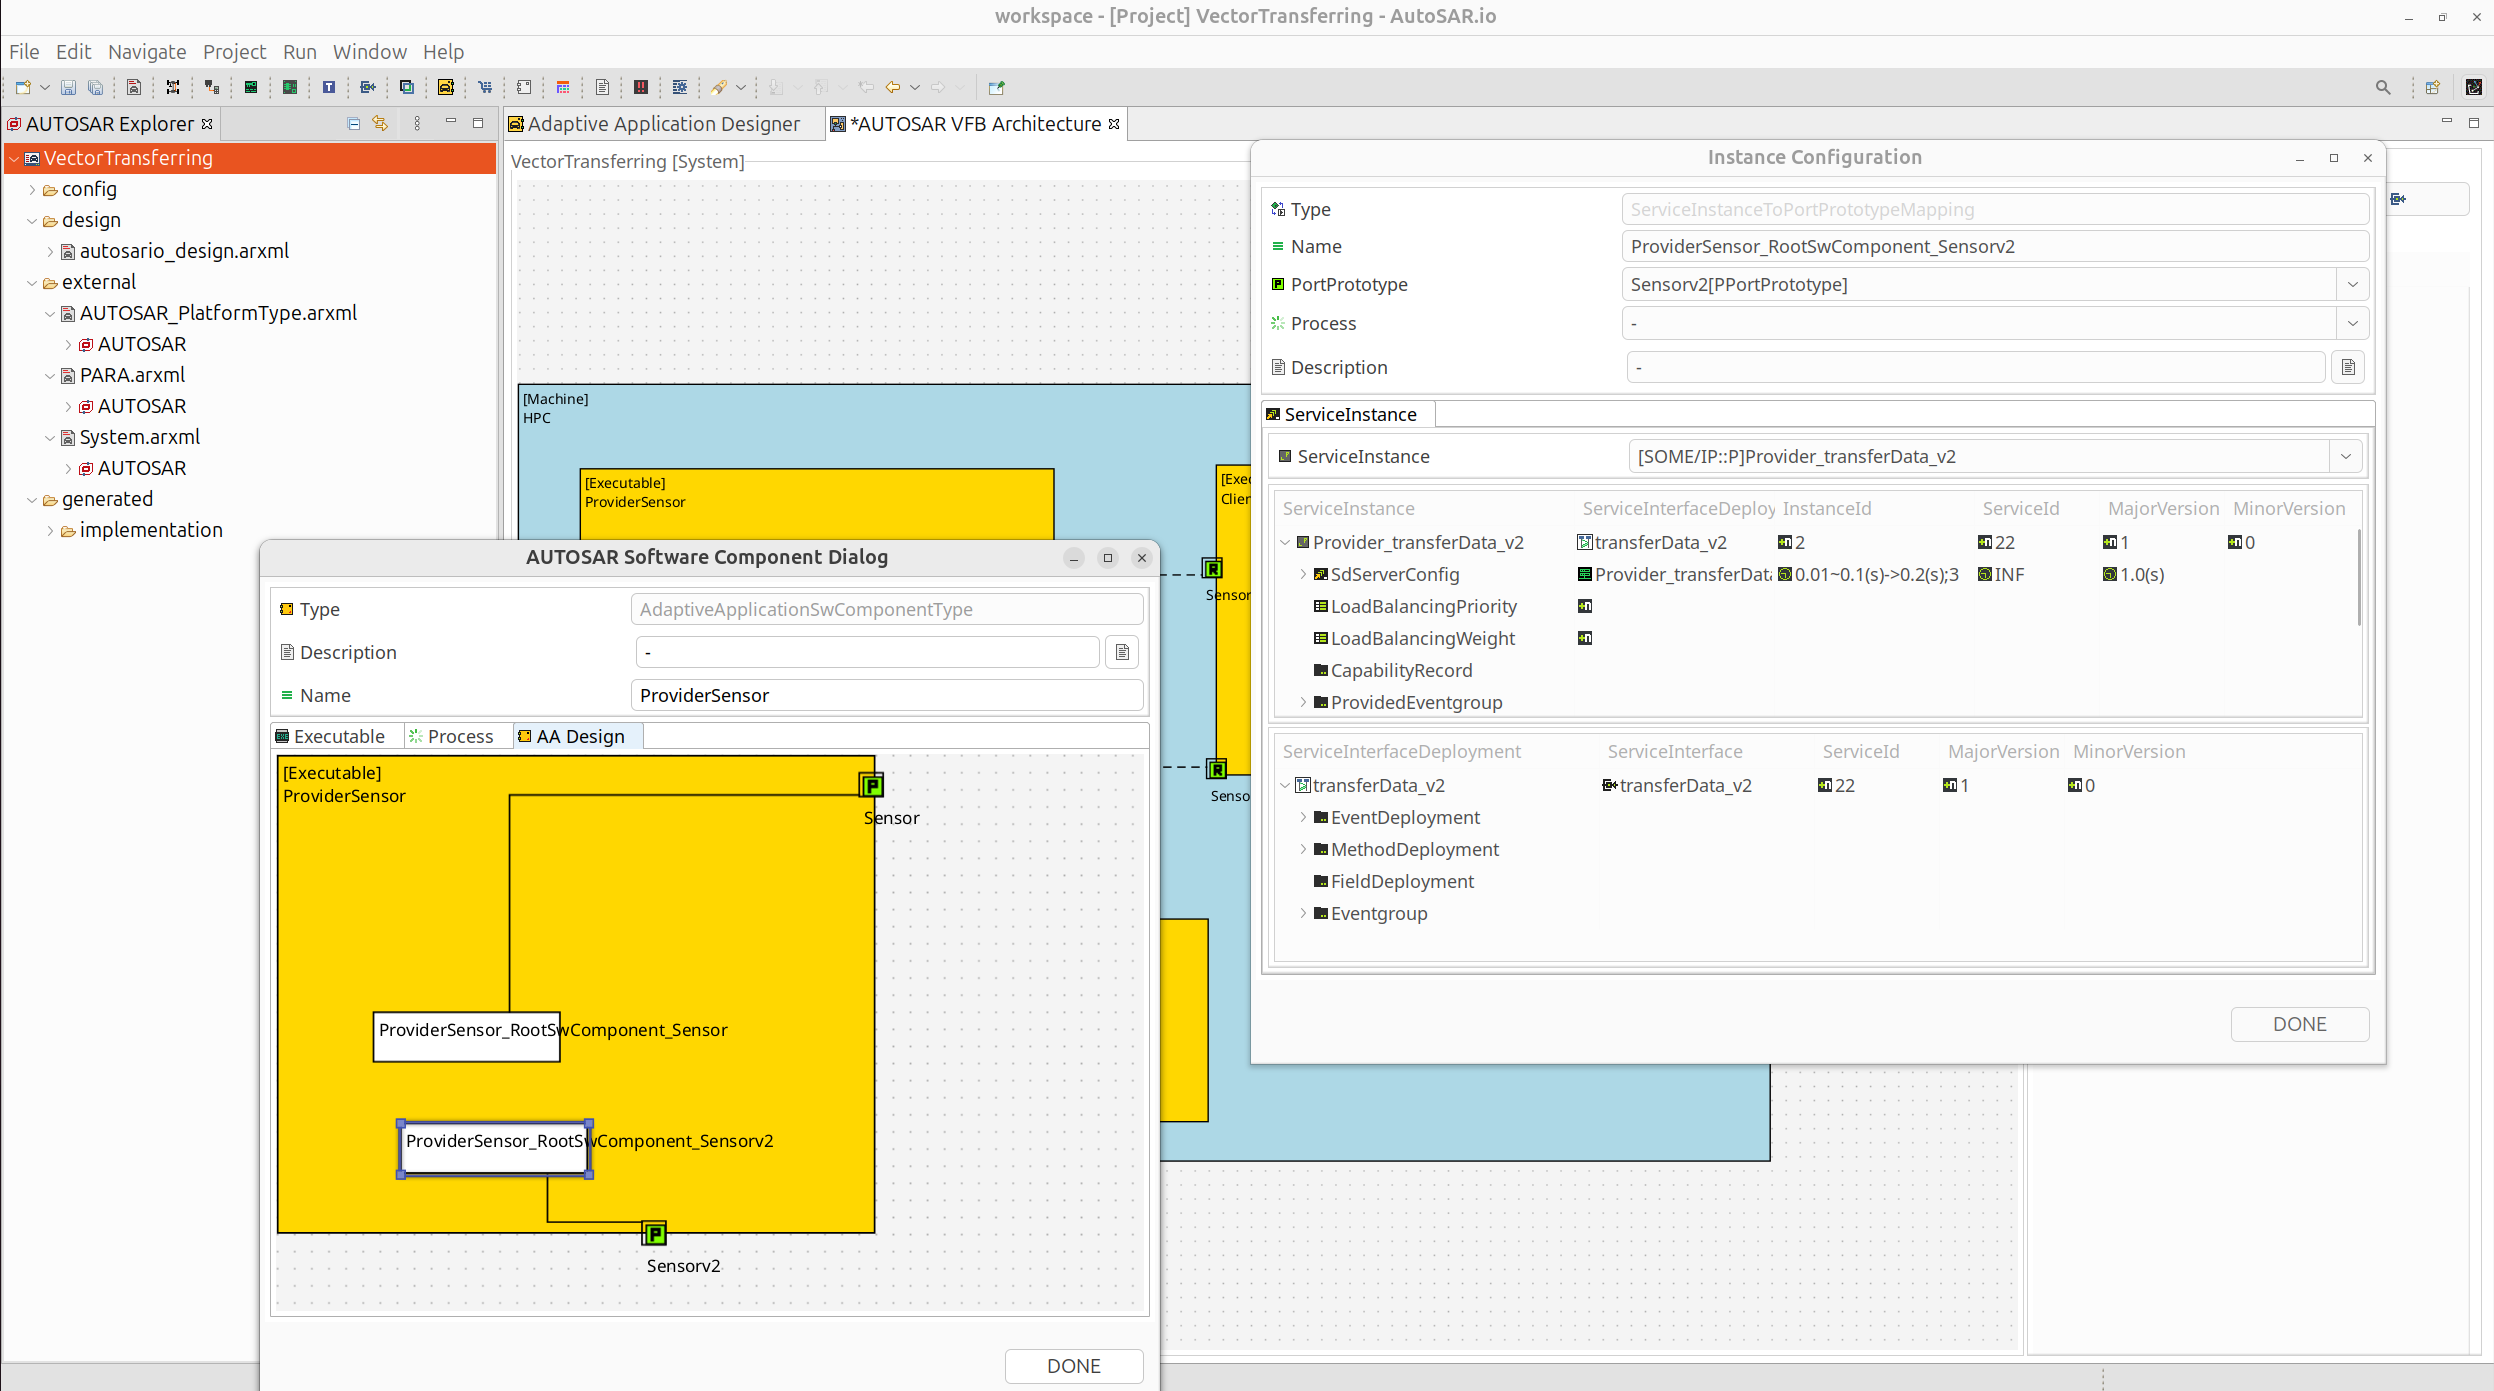
\includegraphics[width=0.75\textwidth]{Images/chap3/image_methodology/applicationDesign/mappingPortProviderEx.png}
    \vspace{0.5cm}
    \caption{Mapping Provider Ports to Service Interface}
    \label{fig:app_mapping_provider_ports}
\end{figure}

Figure~\ref{fig:app_mapping_provider_ports} illustrates the association between the provider executable ports and the previously defined AUTOSAR software component. In this step, the ports of the \texttt{ProviderSensor} executable are mapped to the corresponding port prototypes of the Adaptive Application Software Component that has already been specified in the AUTOSAR model. This configuration establishes a clear link between the executable instance and its software component definition, ensuring that the executable correctly realizes the component’s provided interfaces. As a result, the application implementation becomes consistent with the AUTOSAR architectural model before being bound to concrete service instances and communication middleware.


% Configure Subscriber Executable Properties
\begin{figure}[H]
    \centering
    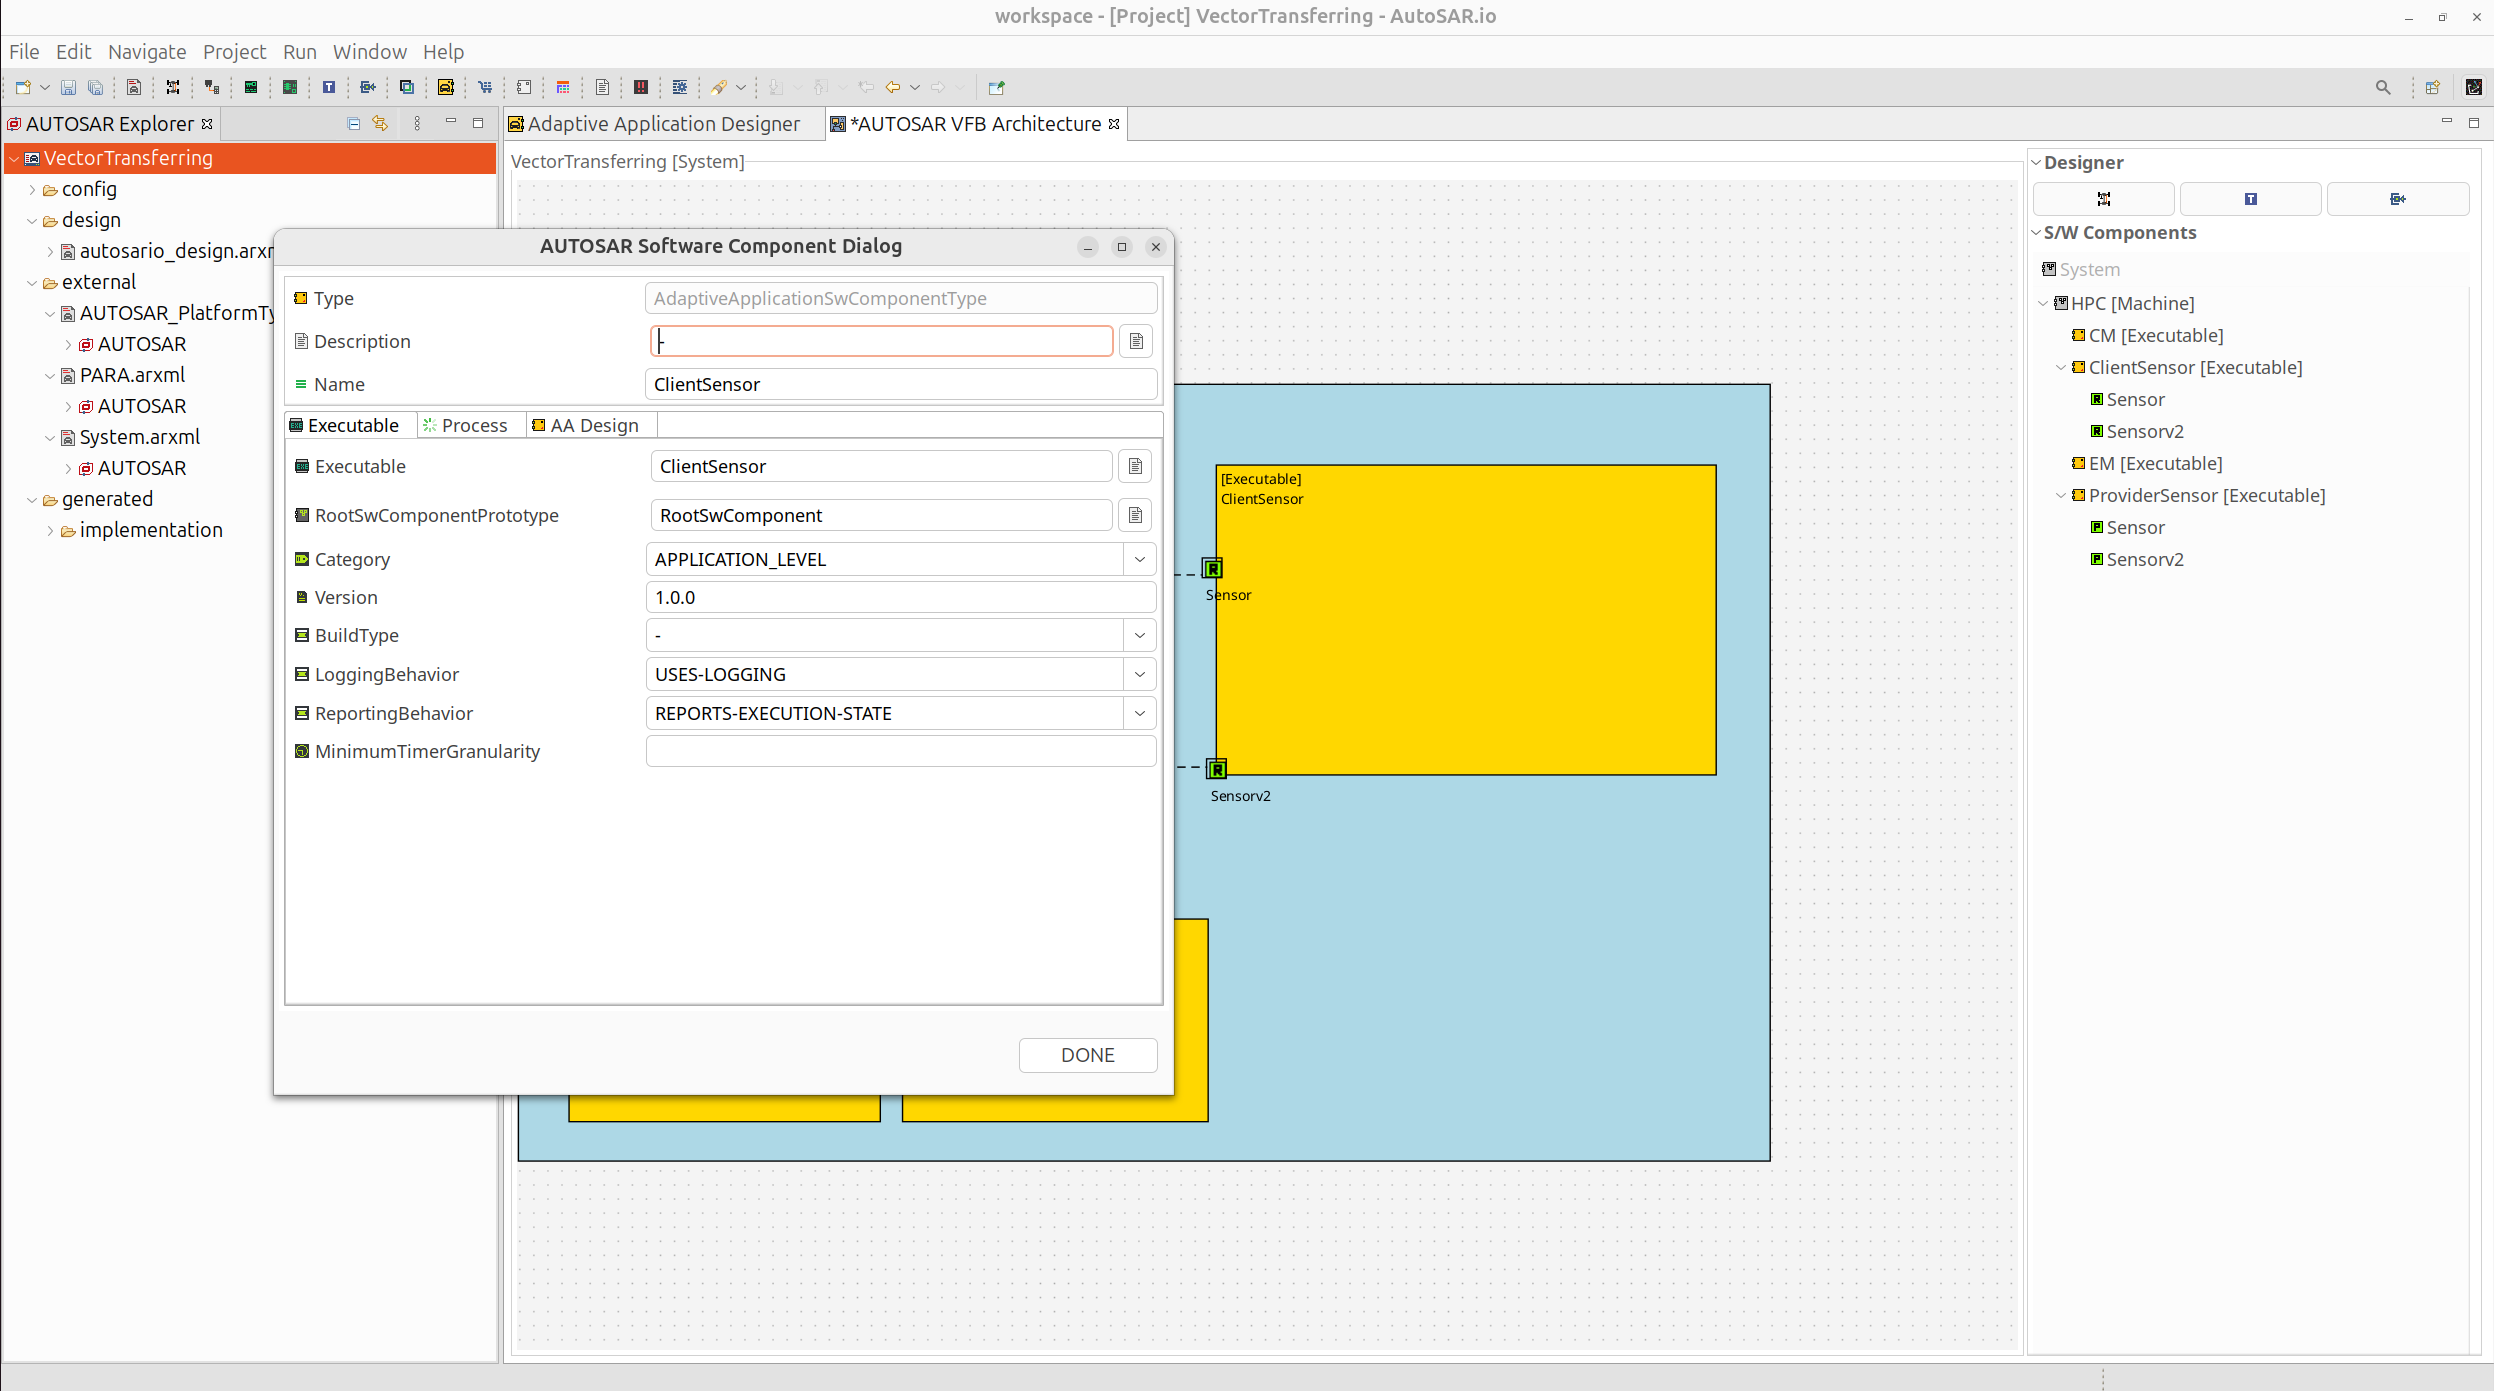
\includegraphics[width=0.75\textwidth]{Images/chap3/image_methodology/applicationDesign/subscriberExProperties.png}
    \vspace{0.5cm}
    \caption{Configuration of Subscriber Executable Properties}
    \label{fig:app_subscriber_executable_properties}
\end{figure}

Figure~\ref{fig:app_subscriber_executable_properties} illustrates the definition of the \texttt{ClientSensor} executable as an adaptive application software component. In this step, the executable is characterized at the application level by specifying its name, version, category, and runtime behavior such as logging and execution state reporting. This configuration formally registers the client application in the AUTOSAR model and establishes it as a runnable entity that can participate in service oriented communication.

% Map Client Ports to Service Interface
\begin{figure}[H]
    \centering
    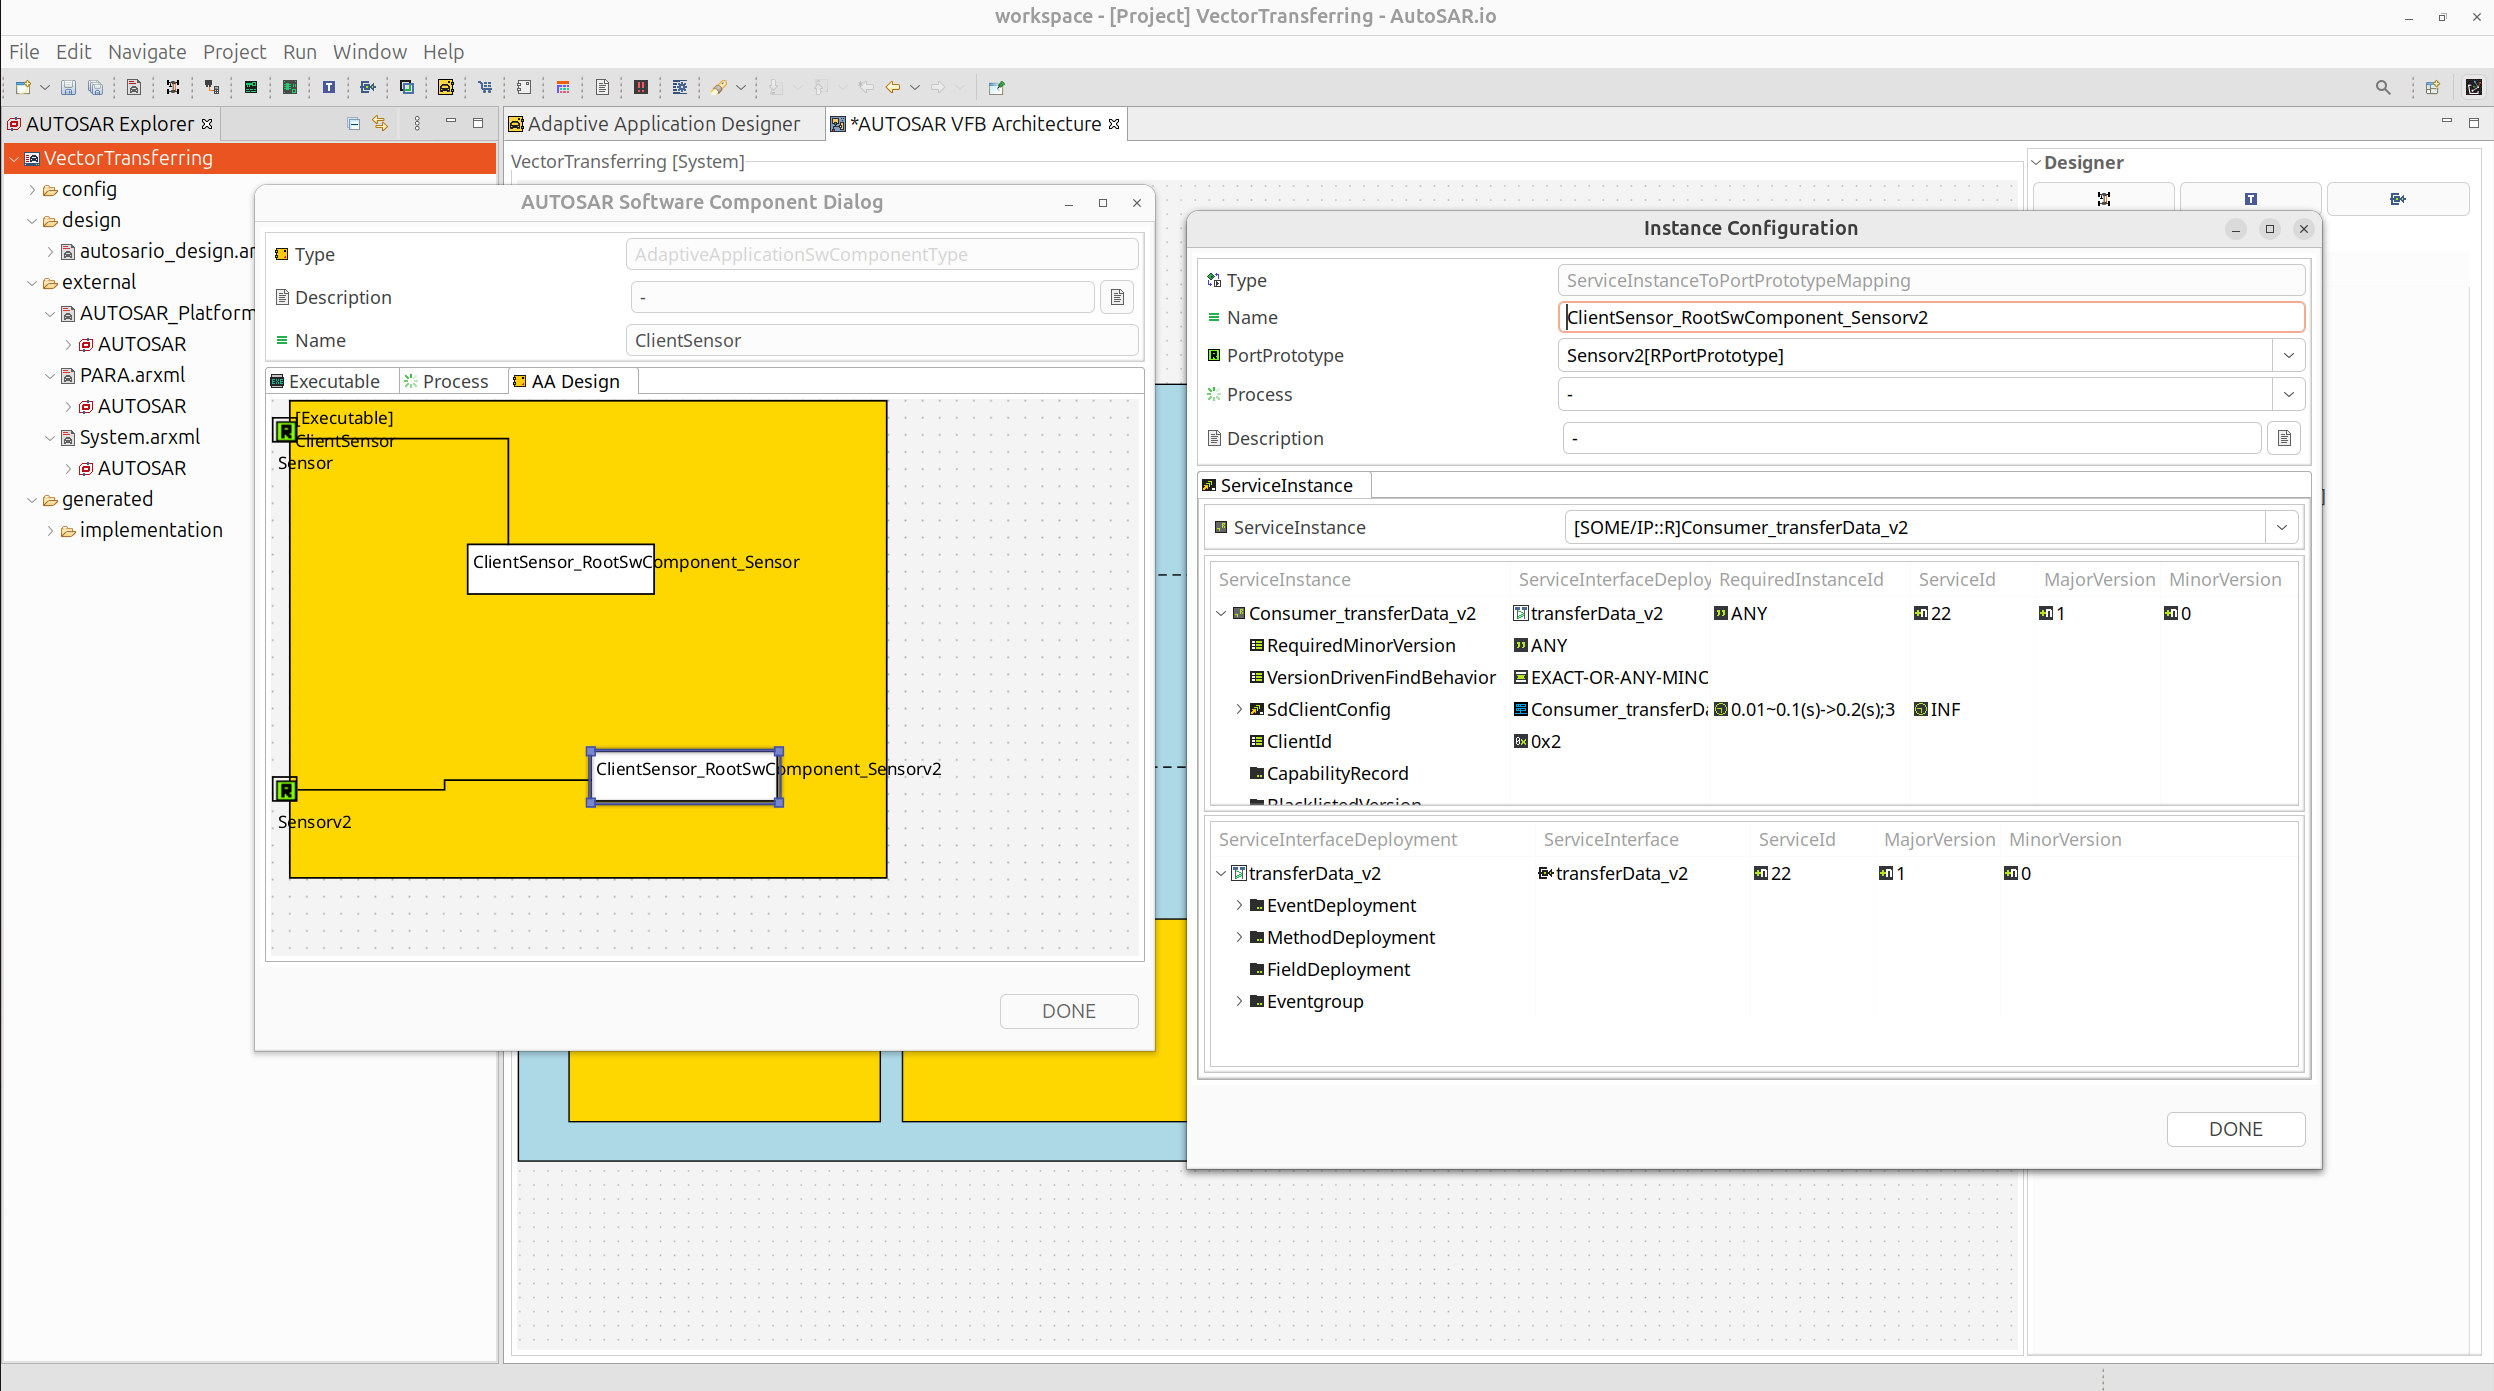
\includegraphics[width=0.75\textwidth]{Images/chap3/image_methodology/applicationDesign/mappingPortClientEx.png}
    \vspace{0.5cm}
    \caption{Mapping Client Ports to Service Interface}
    \label{fig:app_mapping_client_ports}
\end{figure}

As shown in Figure~\ref{fig:app_mapping_client_ports}, the required ports of the \texttt{ClientSensor} software component are then associated with the corresponding port prototypes defined in the AUTOSAR architecture. This association links the client implementation to the abstract interface contracts specified at design time, without directly binding it to network level details. By completing this step, the client executable is structurally aligned with the AUTOSAR software component model, enabling subsequent binding to concrete service instances during service deployment and machine mapping.

% Configure Application Startup Behavior
\begin{figure}[H]
    \centering
    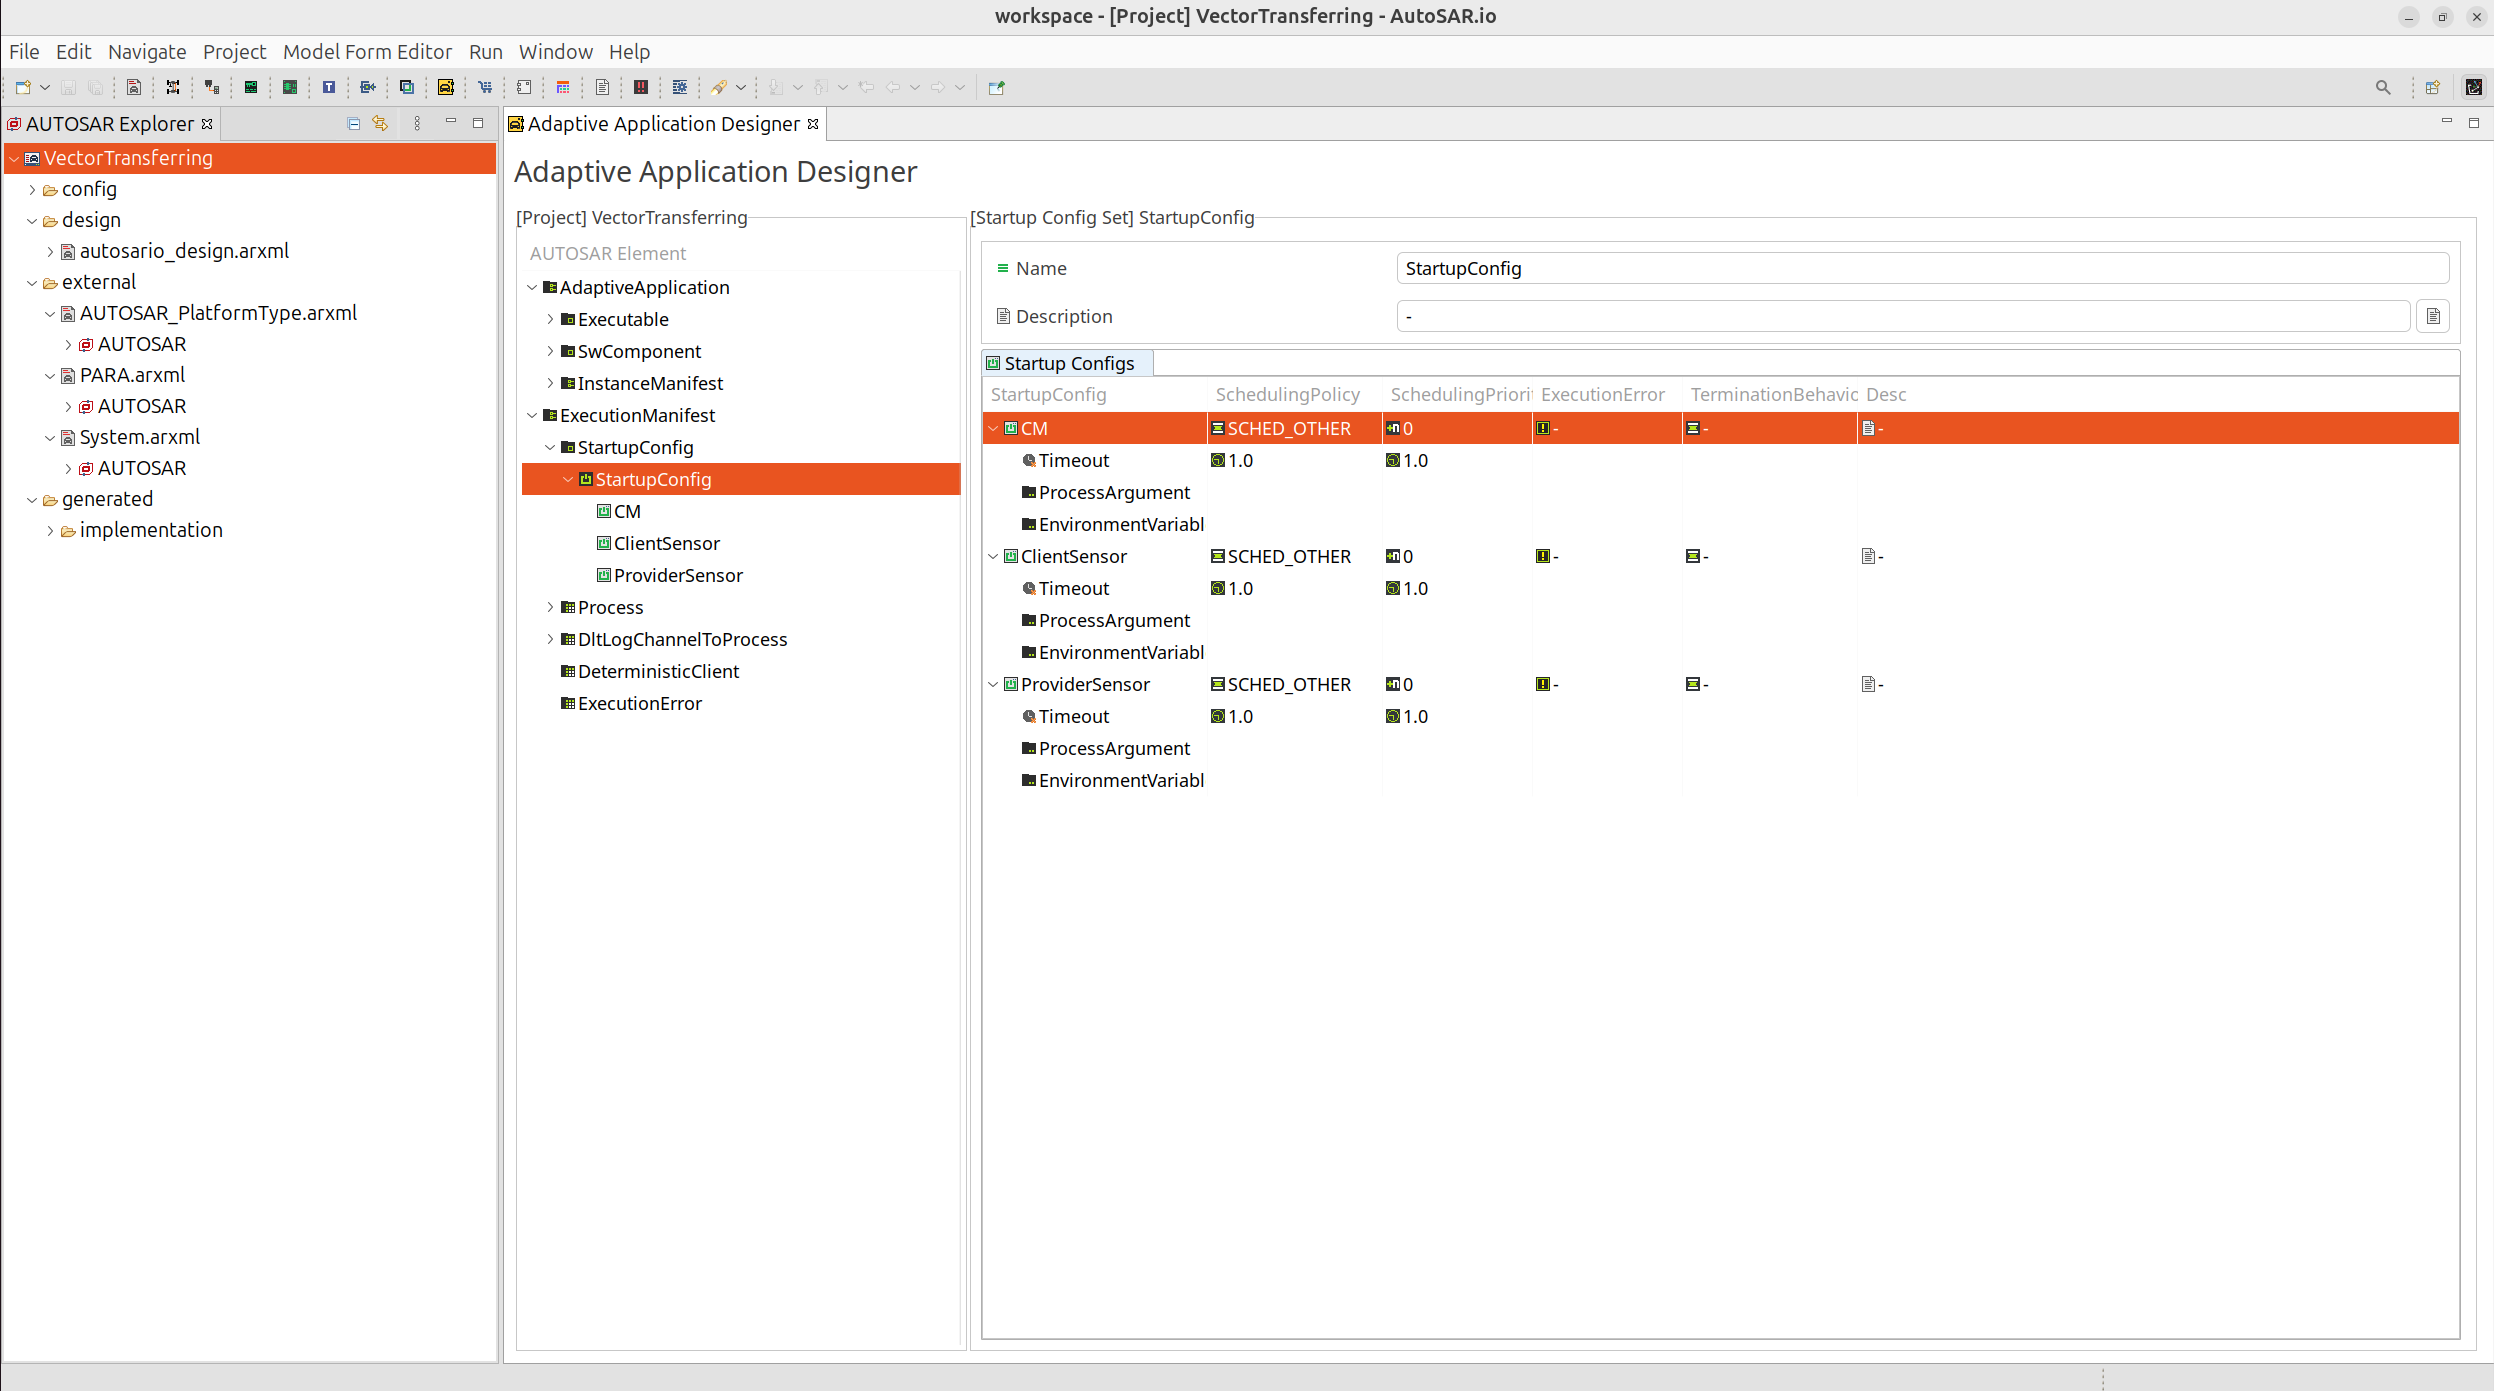
\includegraphics[width=0.75\textwidth]{Images/chap3/image_methodology/applicationDesign/configureStartupConfigure.png}
    \vspace{0.5cm}
    \caption{Configuration of Application Startup Behavior}
    \label{fig:app_startup_configuration}
\end{figure}

Figure~\ref{fig:app_startup_configuration} illustrates the startup configuration set that governs how adaptive application processes are initialized on the target platform. Each process, including \texttt{CM}, \texttt{ClientSensor}, and \texttt{ProviderSensor}, is assigned a scheduling policy and priority, ensuring consistent execution behavior under the POSIX based operating environment. The use of a unified scheduling class allows the platform to manage multiple applications in a predictable manner during system boot.

In addition, the startup configuration defines timeout values and process level parameters that control execution supervision at launch time. By explicitly specifying these attributes, the system ensures that all applications enter a well defined initial state and comply with platform execution constraints. This configuration plays a critical role in coordinating application startup with function group transitions and provides a stable foundation for subsequent runtime interactions.

% Bind DLT Channels to Application Processes
\begin{figure}[H]
    \centering
    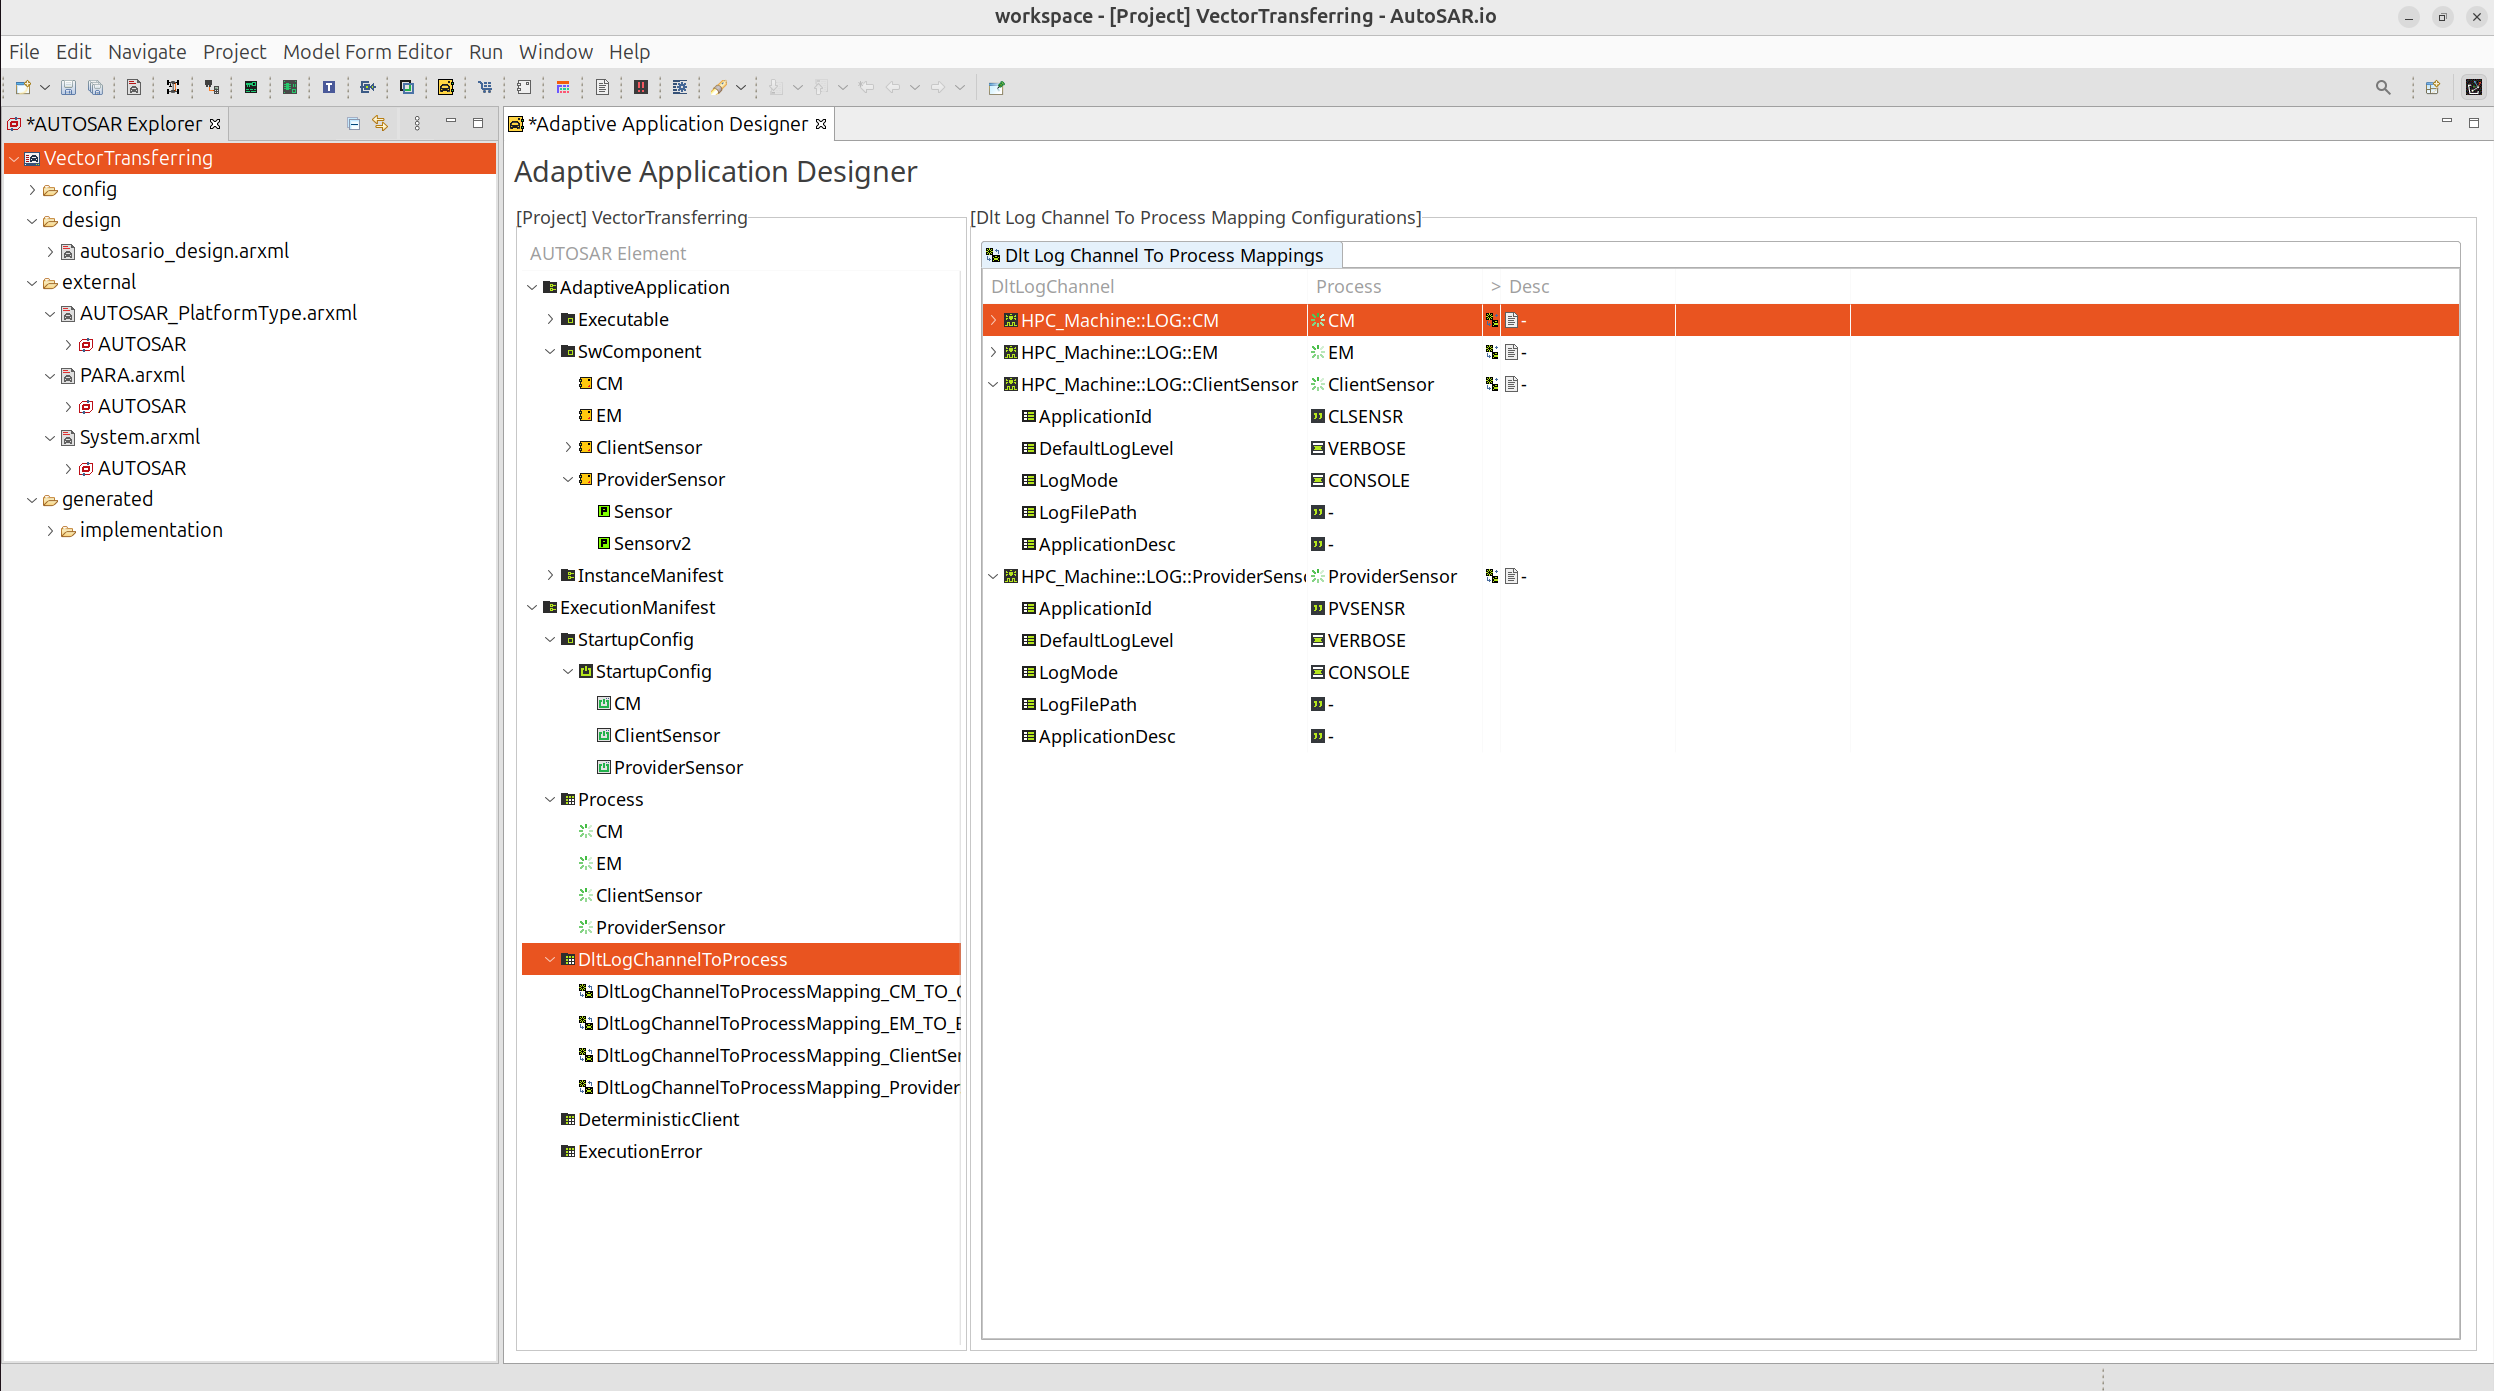
\includegraphics[width=0.75\textwidth]{Images/chap3/image_methodology/applicationDesign/configureDLTChanneltoProcess.png}
    \vspace{0.5cm}
    \caption{Binding Diagnostic Log and Trace Channels to Application Processes}
    \label{fig:app_dlt_process_mapping}
\end{figure}

Figure~\ref{fig:app_dlt_process_mapping} depicts the association between Diagnostic Log and Trace channels and individual application processes. Each process is connected to a specific DLT channel with defined log levels and output modes, enabling consistent monitoring and debugging at runtime. This mapping ensures that diagnostic information is traceable per application, which supports efficient analysis and maintenance in Adaptive AUTOSAR deployments.

% Configure Provider Application Process
\begin{figure}[H]
    \centering
    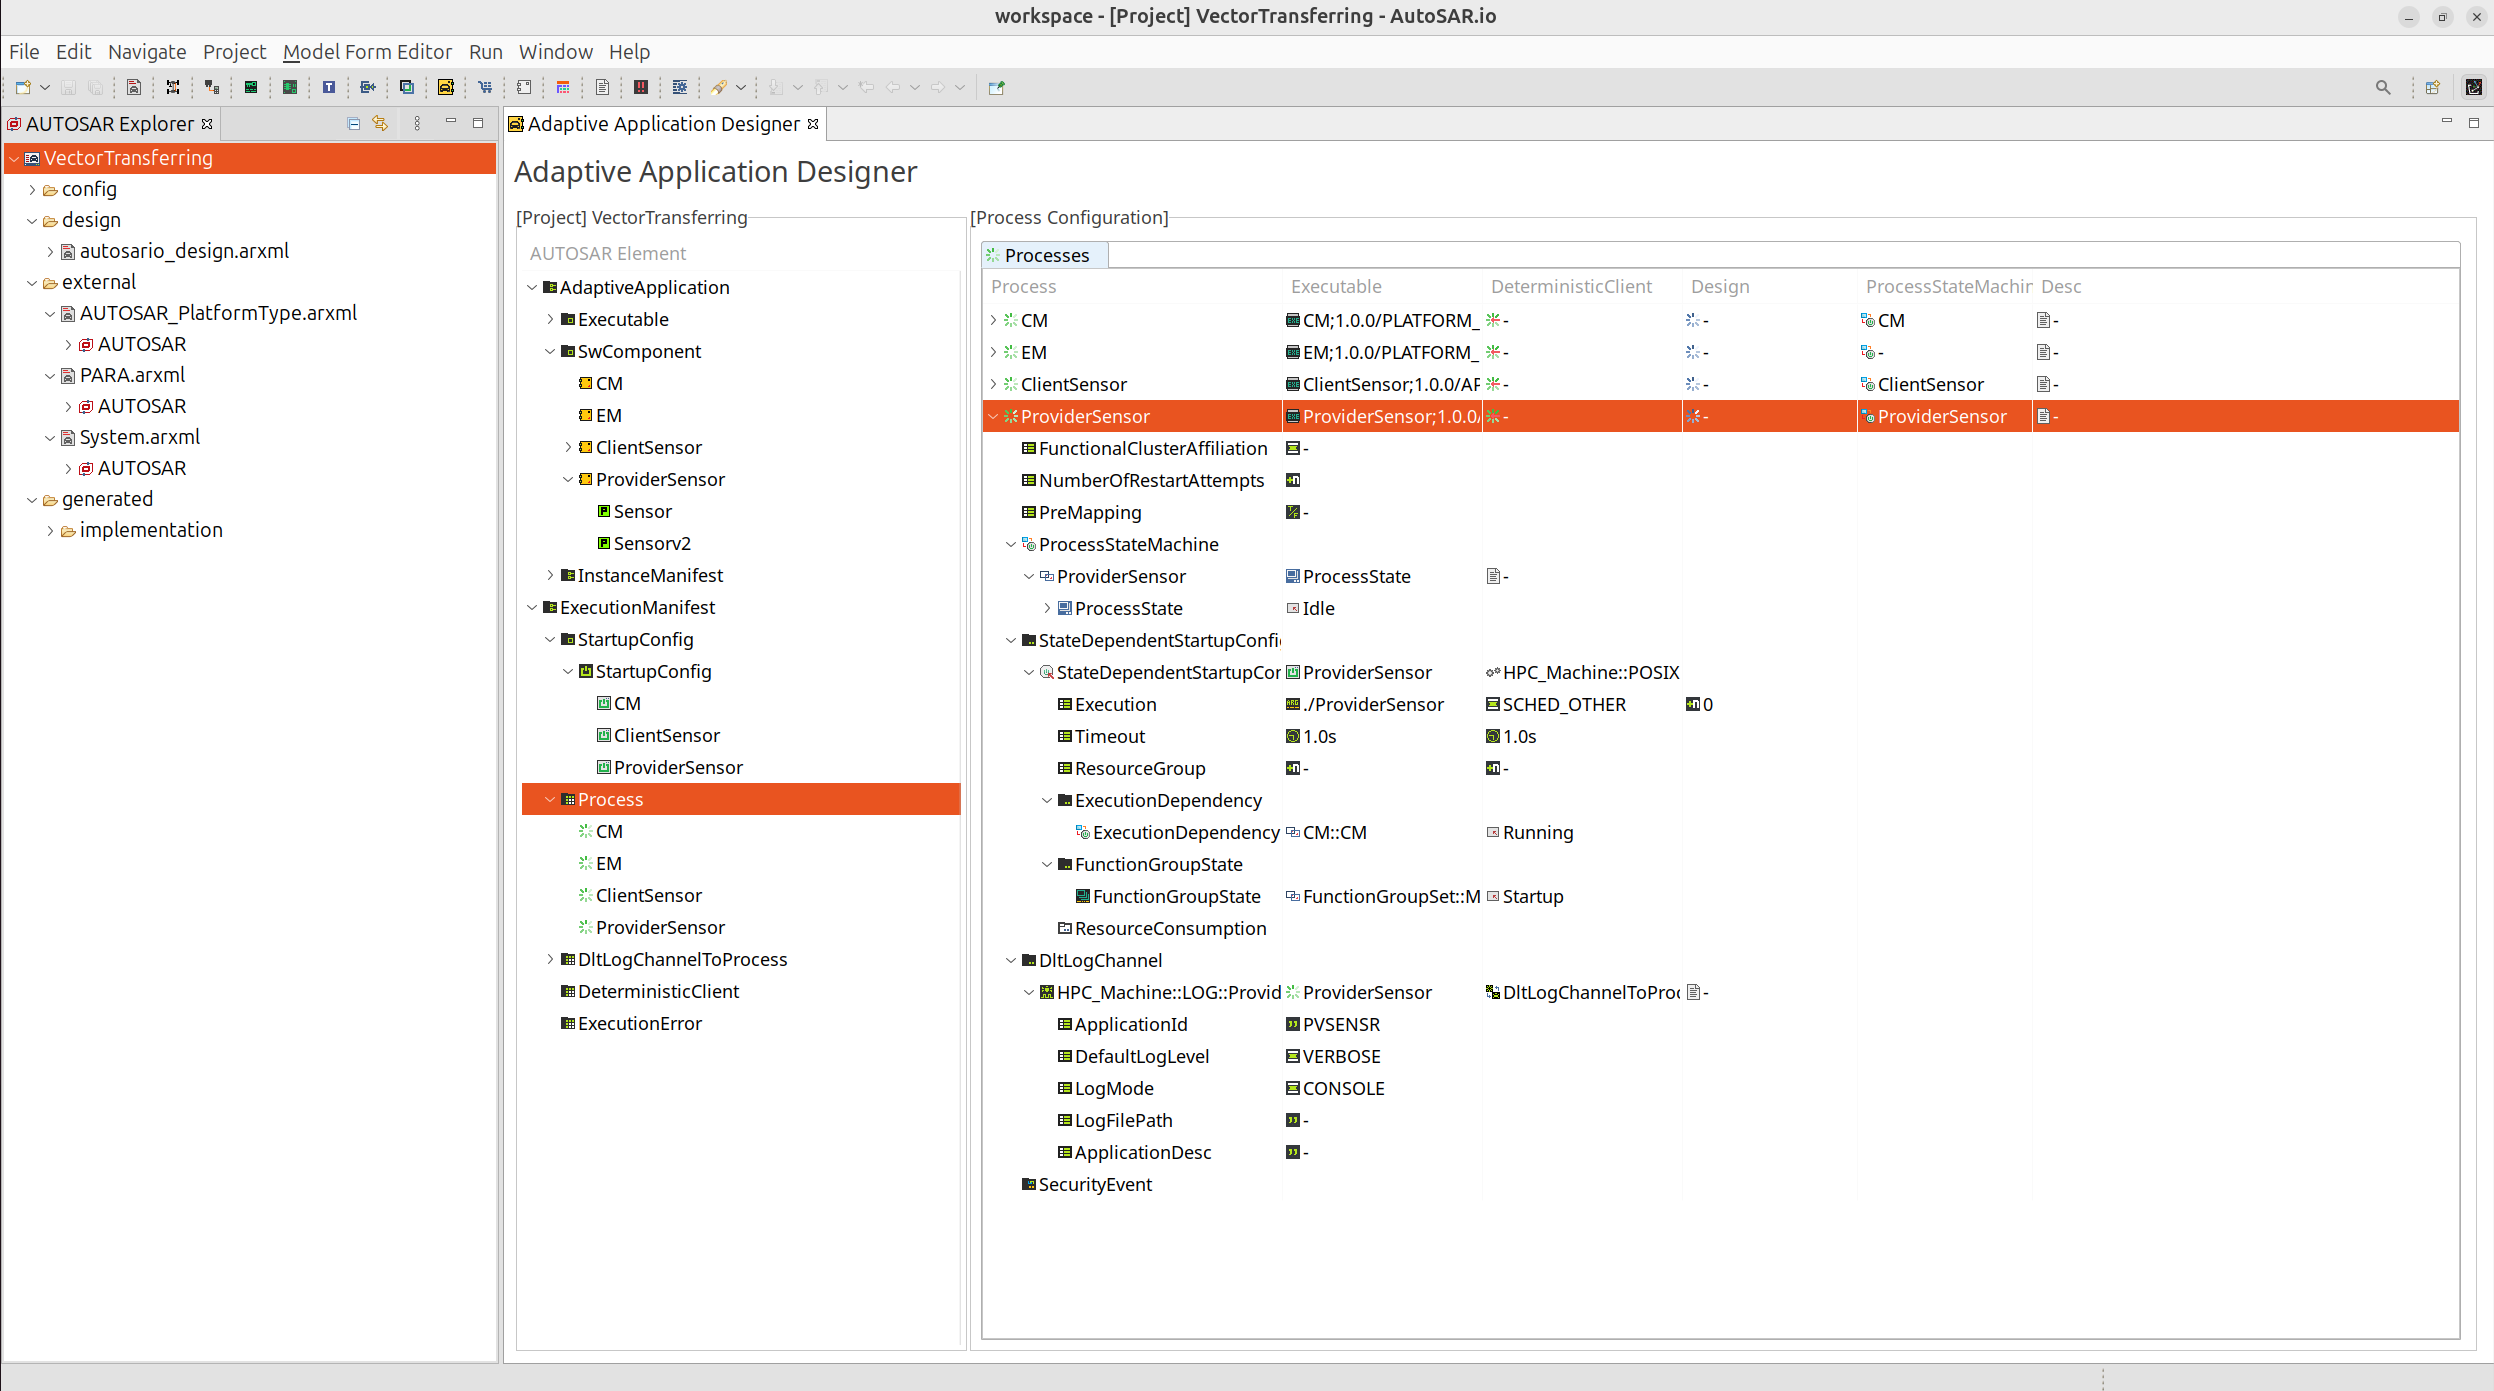
\includegraphics[width=0.75\textwidth]{Images/chap3/image_methodology/applicationDesign/configureProviderProcess.png}
    \vspace{0.5cm}
    \caption{Configuration of Provider Application Process}
    \label{fig:app_provider_process_configuration}
\end{figure}

As illustrated in Figure~\ref{fig:app_provider_process_configuration}, the provider application process is configured by linking the \texttt{ProviderSensor} executable to a dedicated process entity. This step specifies process level attributes such as restart policy, execution dependency, and state machine association, which together describe how the provider behaves during runtime transitions. The configuration clarifies the provider’s role in the execution flow and its dependency on platform level services.

% Configure Client Application Process
\begin{figure}[H]
    \centering
    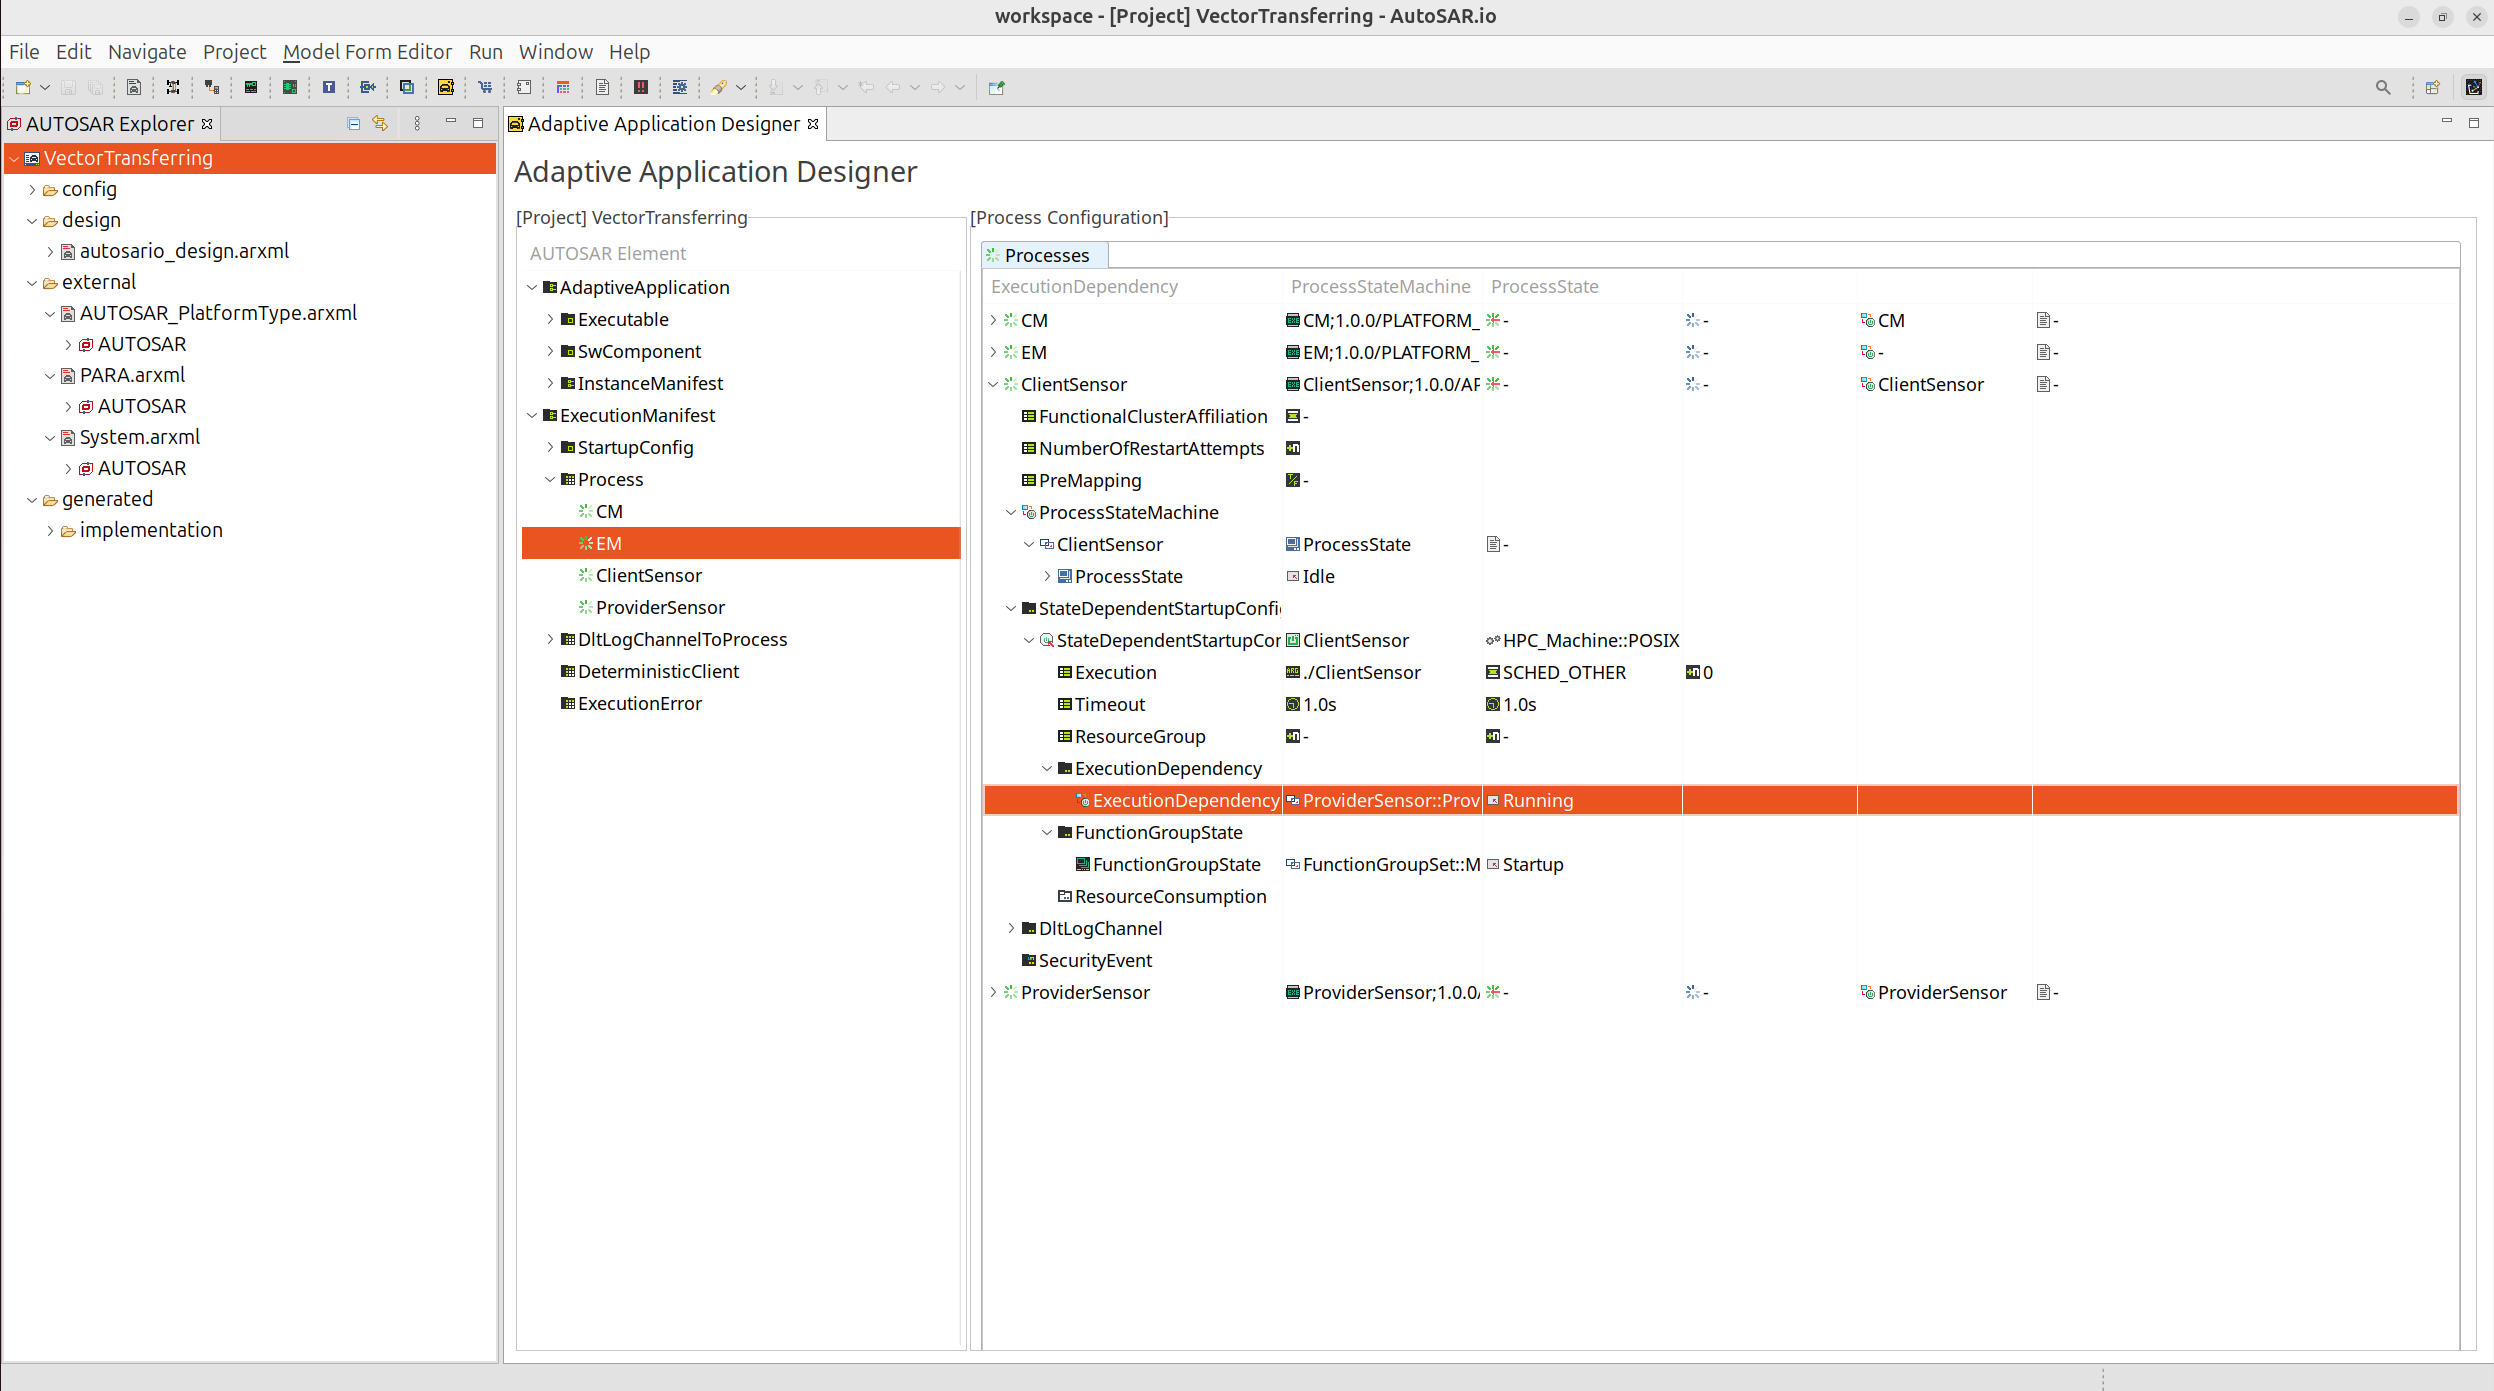
\includegraphics[width=0.75\textwidth]{Images/chap3/image_methodology/applicationDesign/configureClientProcess.png}
    \vspace{0.5cm}
    \caption{Configuration of Client Application Process}
    \label{fig:app_client_process_configuration}
\end{figure}

Figure~\ref{fig:app_client_process_configuration} shows a similar setup for the client application, where the \texttt{ClientSensor} executable is bound to its own process instance. Here, execution states and startup dependencies are defined to ensure that the client is activated only when required conditions are satisfied. This separation at the process level improves modularity and allows independent management of client and provider lifecycles.

% Map Application Processes to Target Machine
\begin{figure}[H]
    \centering
    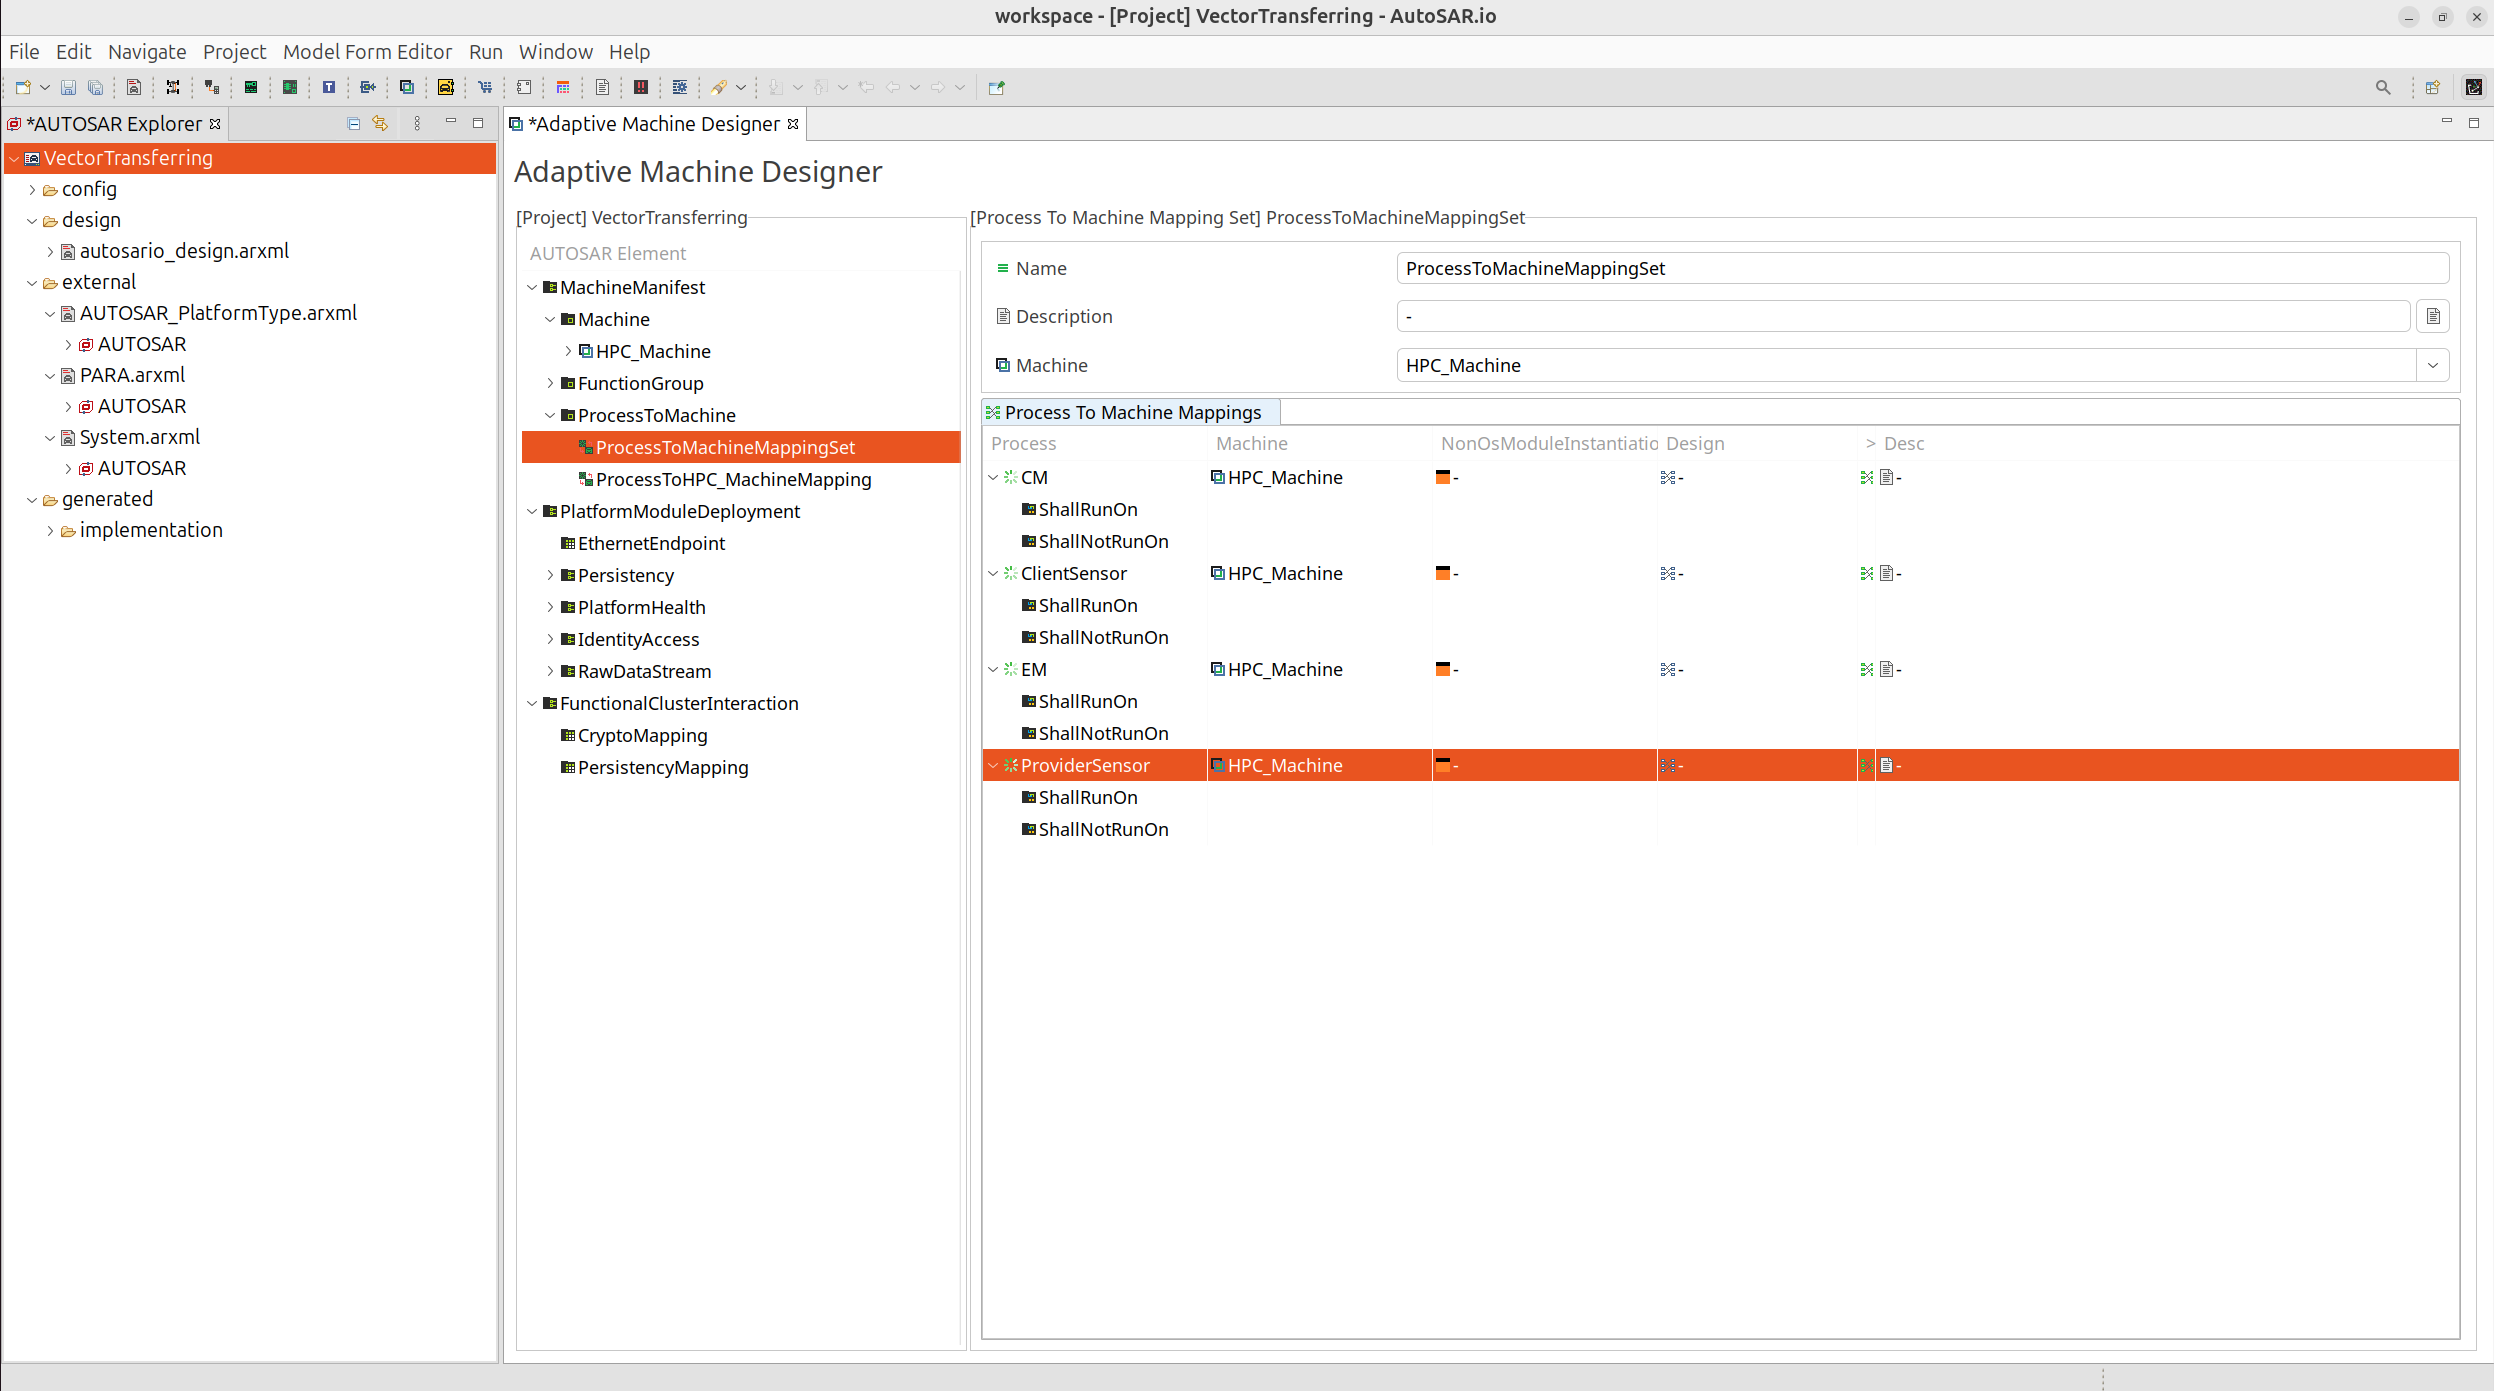
\includegraphics[width=0.75\textwidth]{Images/chap3/image_methodology/applicationDesign/mappingProcesstoMachine.png}
    \vspace{0.5cm}
    \caption{Mapping Application Processes to Target Machine}
    \label{fig:app_process_machine_mapping}
\end{figure}

Finally, Figure~\ref{fig:app_process_machine_mapping} presents the process-to-machine mapping defined in the Adaptive Machine Designer. In this step, all application processes, including \texttt{CM}, \texttt{EM}, \texttt{ClientSensor}, and \texttt{ProviderSensor}, are explicitly assigned to the target \texttt{HPC\_Machine}. This mapping determines the physical execution location of each process and establishes the final deployment relationship between the adaptive applications and the underlying hardware platform.

By consolidating all processes onto a single machine, the configuration ensures a coherent execution environment and simplifies resource management during runtime. This step completes the application deployment workflow by bridging the gap between application-level process definitions and machine-level execution, enabling the Adaptive AUTOSAR runtime to launch and supervise each process according to the previously defined startup, scheduling, and communication configurations.

\subsubsection{Generating Code and Manifest Files}
After completing the configuration steps at the machine, service, and application levels, the Autosar.io tool supports automatic generation of implementation artifacts through the PARA Generator. This generator collects all previously defined models, including Machine Manifests, service definitions, service instances, and application processes, and transforms them into deployable outputs that conform to the Adaptive AUTOSAR specification. By doing so, the tool ensures that the system configuration remains consistent from design time to implementation.

\begin{figure}[H]
    \centering
    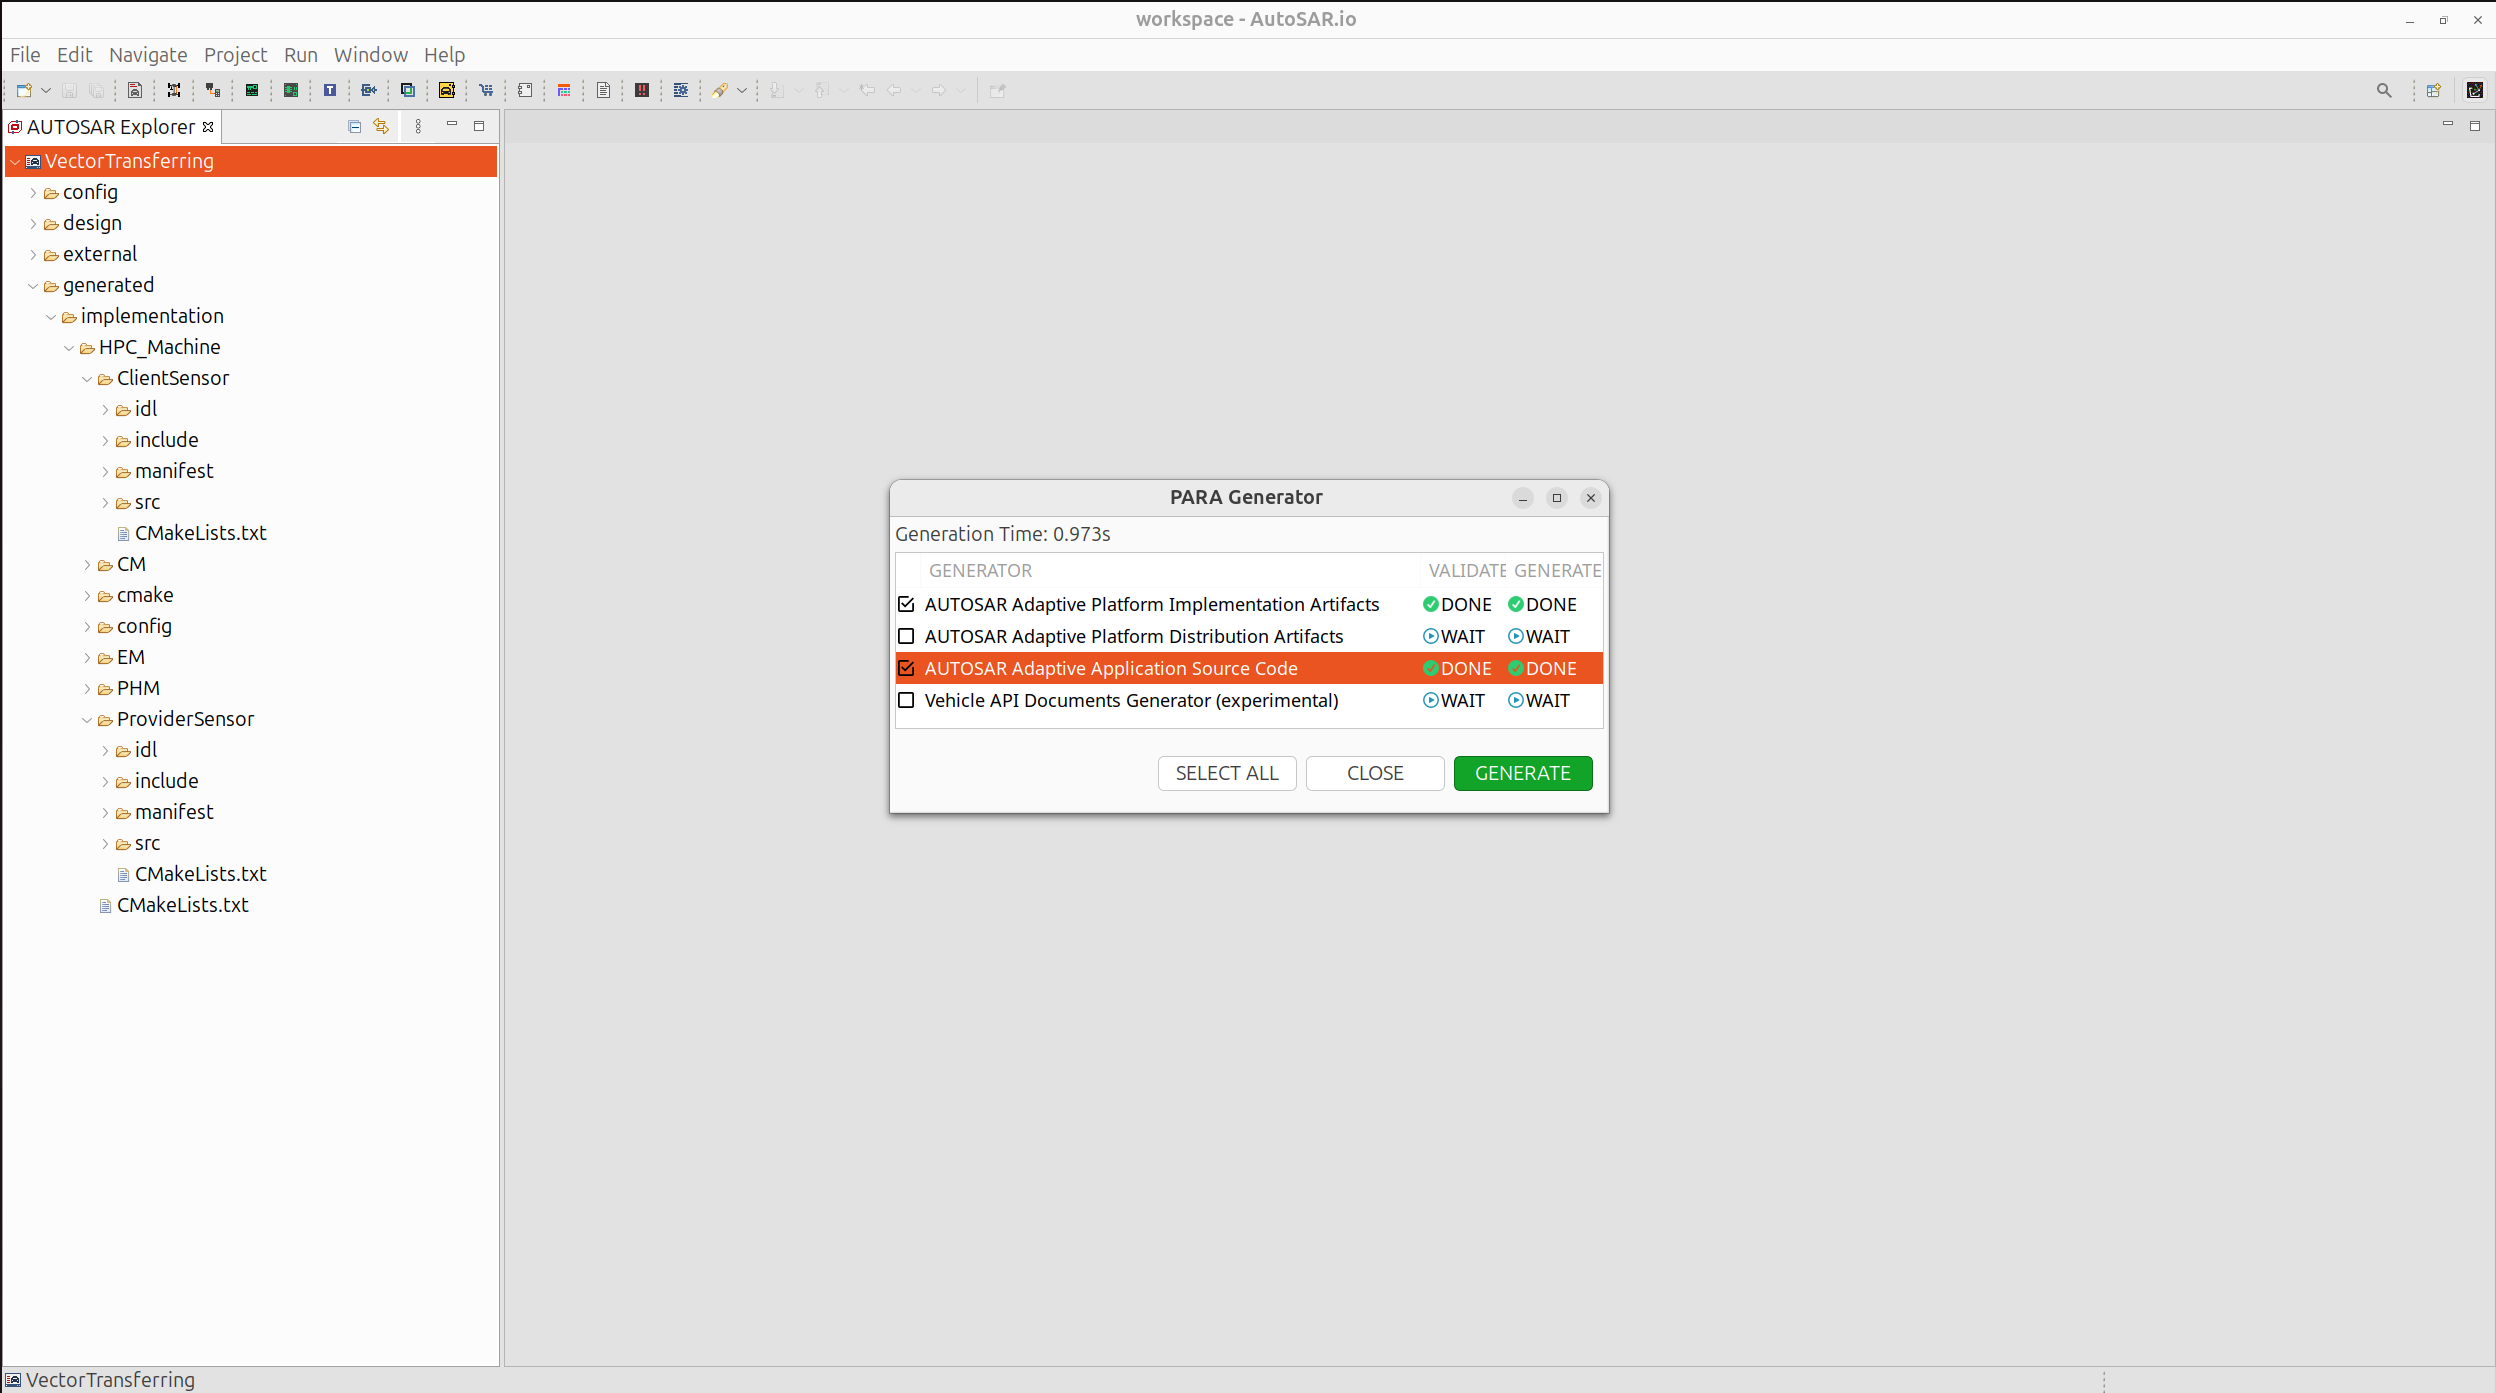
\includegraphics[width=0.75\textwidth]{Images/chap3/generating.png}
    \vspace{0.5cm}
    \caption{Generating Code and ARXML Files}
    \label{fig:code_generation}
\end{figure}

As illustrated in Figure~\ref{fig:code_generation}, the PARA Generator allows users to selectively generate different categories of artifacts, such as Adaptive Application source code, platform configuration files, and manifest descriptions. The generation process produces AUTOSAR compliant ARXML files together with structured C++ source code for each executable. These outputs follow a standardized directory layout, which simplifies subsequent build and integration steps.

Through this automated generation mechanism, Autosar.io bridges the gap between high level system modeling and concrete software artifacts. The generated code and configuration files serve as a reliable foundation for compilation, deployment, and runtime execution. This approach reduces manual errors, improves traceability, and supports a smooth transition from configuration to system integration in the Adaptive AUTOSAR development workflow.

% After establishing the Adaptive AUTOSAR configuration workflow, the system still requires a perception model capable of detecting traffic lights in real time. Therefore, the next subsection shifts from platform configuration to the design and training of the YOLO-MobileNetV4 model. This connection shows how the configured software architecture is supported by an edge-oriented AI component.

% % In this work, we adopt a customized version of the YOLO detection framework by integrating the MobileNetV4 backbone in order to obtain a lightweight yet effective object detection model. The primary motivation behind this design choice is to reduce computational complexity and memory consumption while maintaining reliable detection accuracy. Such requirements are essential for deployment on resource constrained edge devices, including embedded systems, single board computers, and mobile platforms.

% MobileNetV4 is a recently proposed convolutional neural network architecture designed for universal deployment across mobile and edge hardware. It emphasizes efficient feature extraction through improved depthwise separable convolutions, universal inverted bottleneck blocks, and optimized layer scaling strategies. Compared to conventional backbones such as CSPDarknet or standard ResNet variants, MobileNetV4 provides a more balanced trade off between inference speed and representational capability. As a result, it is particularly suitable for real time computer vision tasks where latency, power consumption, and memory footprint are critical constraints.

% \subsection{Backbone Replacement Strategy}

% To integrate MobileNetV4 into the YOLO framework, the default backbone definition is replaced by a customized model configuration file, denoted as \texttt{yolo11-mobilenetv4.yaml}. This configuration follows the standard Ultralytics YOLO model definition format while modifying the backbone section to incorporate MobileNetV4 building blocks. The neck and detection head structures remain largely unchanged in order to preserve compatibility with existing loss functions, anchor settings, and training pipelines.

% The backbone replacement process is performed at the model configuration and module registration level rather than modifying the core training logic. This design choice improves maintainability and simplifies future updates of the YOLO framework. The integration procedure follows a publicly available technical guide that details how MobileNetV4 modules are registered, parsed, and treated as backbone components during model construction\footnote{Guideline for integrating MobileNetV4 into YOLO architectures is available at \url{https://blog.csdn.net/qq_44231797/article/details/147483132}.}. By preserving the feature pyramid structure, multi scale detection capability is maintained despite the lightweight backbone.

% \subsection{Model Initialization and Pretrained Weights}

% To accelerate convergence and improve training stability, the model is initialized using pretrained weights from a lightweight YOLO variant. Specifically, the \texttt{yolo11n.pt} checkpoint is loaded as the initial parameter set. Although the backbone architecture differs from the original YOLO design, partial weight transfer remains beneficial for shared components such as the detection head and certain convolutional layers.

% The Ultralytics YOLO API automatically performs parameter matching where possible and ignores incompatible layers. This mechanism enables the model to leverage prior knowledge while avoiding structural conflicts during initialization. As a result, the training process converges more reliably compared to training from scratch.

% \subsection{Training Configuration}

% The training process is conducted using the Ultralytics YOLO training interface, which provides a flexible and reproducible pipeline for object detection tasks. Dataset information is specified through a YAML configuration file that defines training and validation paths, class labels, and metadata. All input images are resized to a resolution of $320 \times 320$ pixels in order to balance detection accuracy and computational efficiency.

% Stochastic Gradient Descent is selected as the optimization algorithm due to its stable convergence behavior for large scale detection models. Automatic mixed precision is enabled to reduce GPU memory usage and accelerate training while maintaining numerical stability. The model is trained for a total of 400 epochs to ensure sufficient convergence given the modified backbone structure.

% \subsection{Training Script}

% The complete training script used in this study is shown below. This script defines the model configuration, loads pretrained weights, and executes the training process with the selected hyperparameters.

% \begin{lstlisting}[language=Python, caption={YOLO-MobileNetV4 Training Script}]
% # Model configuration file
% model_yaml_path = r"yolo11-mobilenetv4.yaml"

% # Dataset configuration file
% data_yaml_path = r"dataset/data.yaml"

% # Pretrained model
% pre_model_name = "yolo11n.pt"

% import warnings
% warnings.filterwarnings("ignore")

% from ultralytics import YOLO

% if __name__ == "__main__":
%     model = YOLO(model_yaml_path)
%     model.load(pre_model_name)

%     model.train(
%         data=data_yaml_path,
%         cache=False,
%         imgsz=320,
%         epochs=400,
%         workers=8,
%         device="0",
%         optimizer="SGD",
%         amp=True,
%         project="runs/train-yolo-mobilenetv4",
%         name="exp"
%     )
% \end{lstlisting}

\section{YOLO-MobileNetV4 Model}

In this work, we adopt a customized version of the YOLOv26 detection framework by integrating the MobileNetV4 backbone in order to obtain a lightweight yet effective object detection model. The primary motivation behind this design choice is to reduce computational complexity and memory consumption while maintaining reliable detection accuracy. Such requirements are essential for deployment on resource constrained edge devices, including embedded systems, single board computers, and mobile platforms.

\subsection{Integrating MobileNetv4 into YOLO}

Following the our paper in \hyperref[chap:append]{Appendix}, we will continue to integrate MobileNetV4 as the feature extractor for YOLO26 creates a hybrid "YOLO-MNv4" architecture that is theoretically optimal for autonomous driving. On mobile accelerators like the Pixel EdgeTPU, MNv4 is approximately twice as fast as MobileNetV3 for equivalent accuracy due to its high operational intensity. Replacing the standard YOLO26 backbone with MNv4 significantly reduces the floating-point operations (FLOPs) required per inference. This architecture specifically excels in occlusion handling, where the advanced receptive fields of the UIB blocks allow the model to infer the presence of a traffic light even when it is partially obscured by large vehicles, ensuring a robust and reliable perception system.

To adapt the original YOLO26 architecture for edge deployment, several crucial modifications were made (comparing Figure \ref{fig:yolo26_original_arch} to Figure \ref{fig:yolo26_mnv4_arch}). First, the standard heavy CNN backbone was replaced entirely with {MobileNetV4ConvSmall050}. Second, the original 4-head Feature Pyramid Network (P2, P3, P4, P5) was scaled down to a {3-head architecture} (P3, P4, P5) by removing the high-resolution P2 feature extraction path and its corresponding detection head. This reduction dramatically lowers the computational complexity (GFLOPs) and parameter count. Meanwhile, the advanced components of the YOLO26 neck—including the {C3k2} fusion blocks, {SPPF}, {C2PSA} spatial attention, and the {One-to-One Head}-were preserved to maintain state-of-the-art detection logic.

\begin{figure}[htbp]
    \centering
    \resizebox{\textwidth}{!}{
    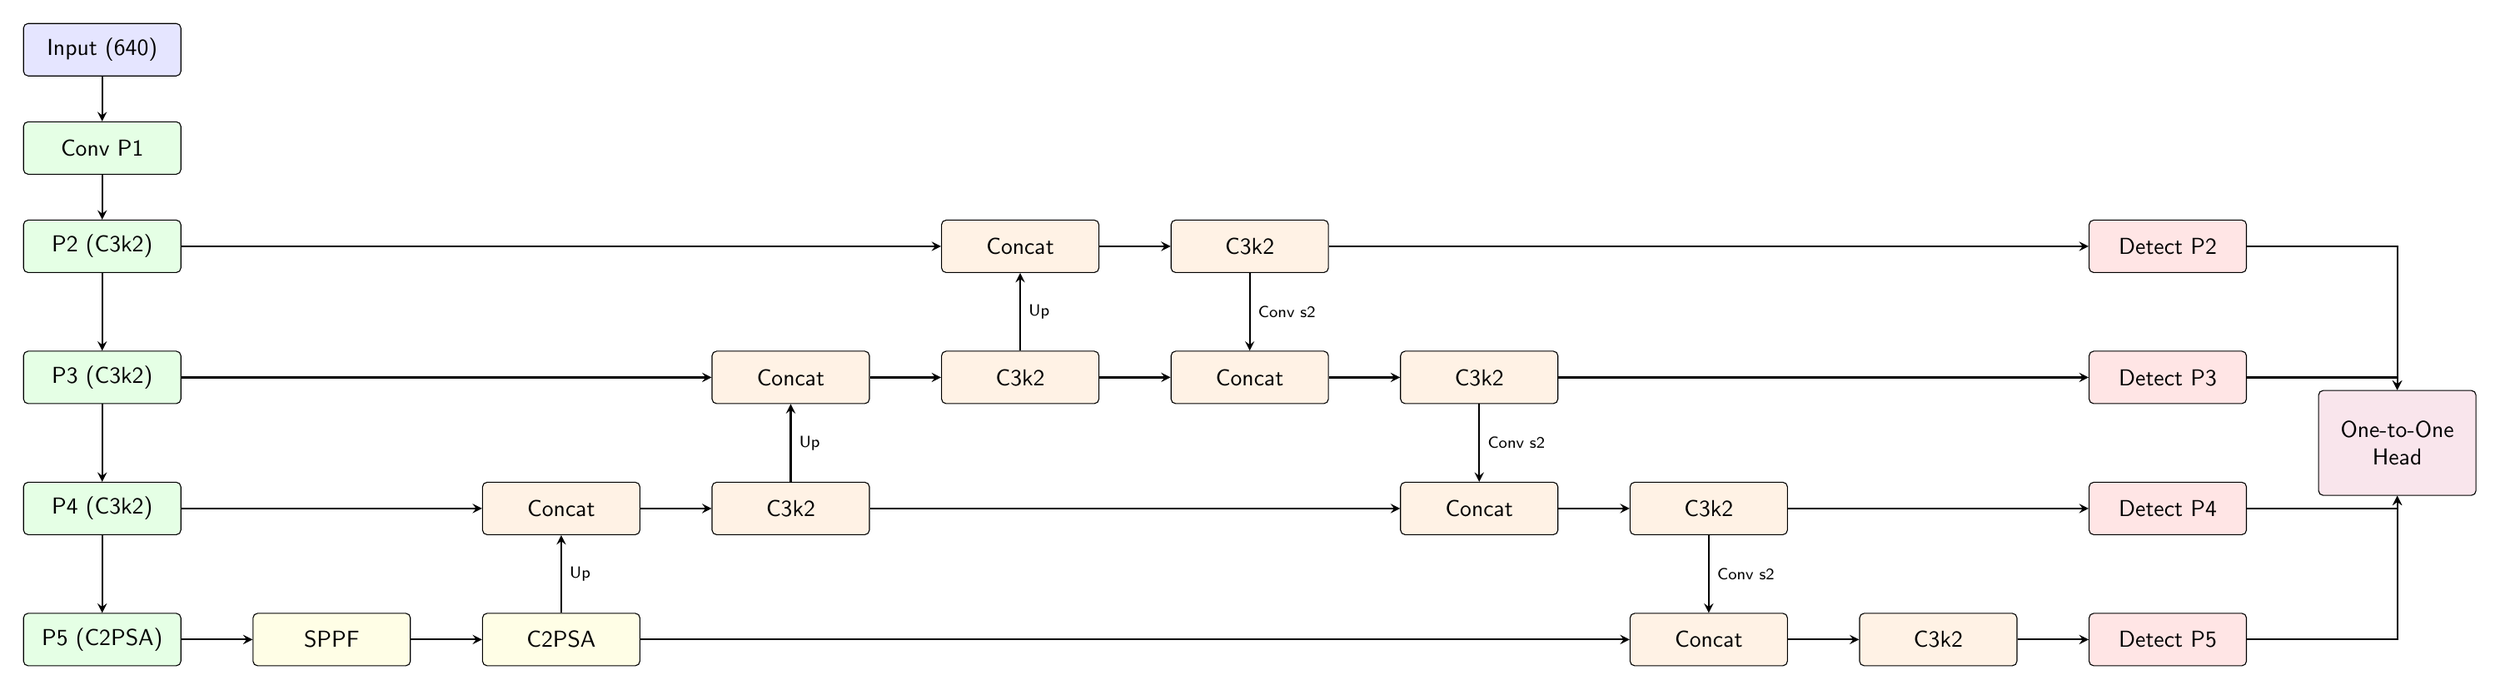
\begin{tikzpicture}[
        box/.style={rectangle, draw, minimum width=2.4cm, minimum height=0.8cm, text centered, font=\sffamily, rounded corners=2pt},
        arrow/.style={->, >=stealth, thick},
        label/.style={font=\sffamily\scriptsize}
    ]

    % Backbone
    \node[box, fill=blue!10] (input) at (0, 9) {Input (640)};
    \node[box, fill=green!10] (conv1) at (0, 7.5) {Conv P1};
    \node[box, fill=green!10] (p2) at (0, 6) {P2 (C3k2)};
    \node[box, fill=green!10] (p3) at (0, 4) {P3 (C3k2)};
    \node[box, fill=green!10] (p4) at (0, 2) {P4 (C3k2)};
    \node[box, fill=green!10] (p5) at (0, 0) {P5 (C2PSA)};

    \draw[arrow] (input) -- (conv1);
    \draw[arrow] (conv1) -- (p2);
    \draw[arrow] (p2) -- (p3);
    \draw[arrow] (p3) -- (p4);
    \draw[arrow] (p4) -- (p5);

    % SPPF & C2PSA
    \node[box, fill=yellow!10] (sppf) at (3.5, 0) {SPPF};
    \node[box, fill=yellow!10] (c2psa) at (7.0, 0) {C2PSA};
    \draw[arrow] (p5) -- (sppf);
    \draw[arrow] (sppf) -- (c2psa);

    % Neck - Top-down
    \node[box, fill=orange!10] (cat_p4) at (7.0, 2) {Concat};
    \node[box, fill=orange!10] (c3k2_td_p4) at (10.5, 2) {C3k2};
    \draw[arrow] (c2psa) -- node[right, label] {Up} (cat_p4);
    \draw[arrow] (p4) -- (cat_p4);
    \draw[arrow] (cat_p4) -- (c3k2_td_p4);

    \node[box, fill=orange!10] (cat_p3) at (10.5, 4) {Concat};
    \node[box, fill=orange!10] (c3k2_td_p3) at (14.0, 4) {C3k2};
    \draw[arrow] (c3k2_td_p4) -- node[right, label] {Up} (cat_p3);
    \draw[arrow] (p3) -- (cat_p3);
    \draw[arrow] (cat_p3) -- (c3k2_td_p3);

    \node[box, fill=orange!10] (cat_p2) at (14.0, 6) {Concat};
    \node[box, fill=orange!10] (c3k2_td_p2) at (17.5, 6) {C3k2};
    \draw[arrow] (c3k2_td_p3) -- node[right, label] {Up} (cat_p2);
    \draw[arrow] (p2) -- (cat_p2);
    \draw[arrow] (cat_p2) -- (c3k2_td_p2);

    % Neck - Bottom-up
    \node[box, fill=orange!10] (cat_p3_bu) at (17.5, 4) {Concat};
    \node[box, fill=orange!10] (c3k2_bu_p3) at (21.0, 4) {C3k2};
    \draw[arrow] (c3k2_td_p2) -- node[right, label] {Conv s2} (cat_p3_bu);
    \draw[arrow] (c3k2_td_p3) -- (cat_p3_bu);
    \draw[arrow] (cat_p3_bu) -- (c3k2_bu_p3);

    \node[box, fill=orange!10] (cat_p4_bu) at (21.0, 2) {Concat};
    \node[box, fill=orange!10] (c3k2_bu_p4) at (24.5, 2) {C3k2};
    \draw[arrow] (c3k2_bu_p3) -- node[right, label] {Conv s2} (cat_p4_bu);
    \draw[arrow] (c3k2_td_p4) -- (cat_p4_bu);
    \draw[arrow] (cat_p4_bu) -- (c3k2_bu_p4);

    \node[box, fill=orange!10] (cat_p5_bu) at (24.5, 0) {Concat};
    \node[box, fill=orange!10] (c3k2_bu_p5) at (28.0, 0) {C3k2};
    \draw[arrow] (c3k2_bu_p4) -- node[right, label] {Conv s2} (cat_p5_bu);
    \draw[arrow] (c2psa) -- (cat_p5_bu);
    \draw[arrow] (cat_p5_bu) -- (c3k2_bu_p5);

    % Detectors
    \node[box, fill=red!10] (head2) at (31.5, 6) {Detect P2};
    \node[box, fill=red!10] (head3) at (31.5, 4) {Detect P3};
    \node[box, fill=red!10] (head4) at (31.5, 2) {Detect P4};
    \node[box, fill=red!10] (head5) at (31.5, 0) {Detect P5};
    
    \node[box, fill=purple!10, align=center, minimum height=1.6cm] (detect) at (35.0, 3) {One-to-One\\Head};

    \draw[arrow] (c3k2_td_p2) -- (head2);
    \draw[arrow] (c3k2_bu_p3) -- (head3);
    \draw[arrow] (c3k2_bu_p4) -- (head4);
    \draw[arrow] (c3k2_bu_p5) -- (head5);
    
    \draw[arrow] (head2) -| (detect);
    \draw[arrow] (head3) -| (detect);
    \draw[arrow] (head4) -| (detect);
    \draw[arrow] (head5) -| (detect);

    \end{tikzpicture}
    }
    \vspace{0.5cm}
    \caption{Architecture of the original YOLO26-p2 model with 4-head detection mechanism (P2/P3/P4/P5 outputs) for standard object detection tasks. Channel widths scale with the chosen model variant (n/s/m/l/x).}
    \label{fig:yolo26_original_arch}
\end{figure}

\begin{figure}[htbp]
    \centering
    \resizebox{\textwidth}{!}{
    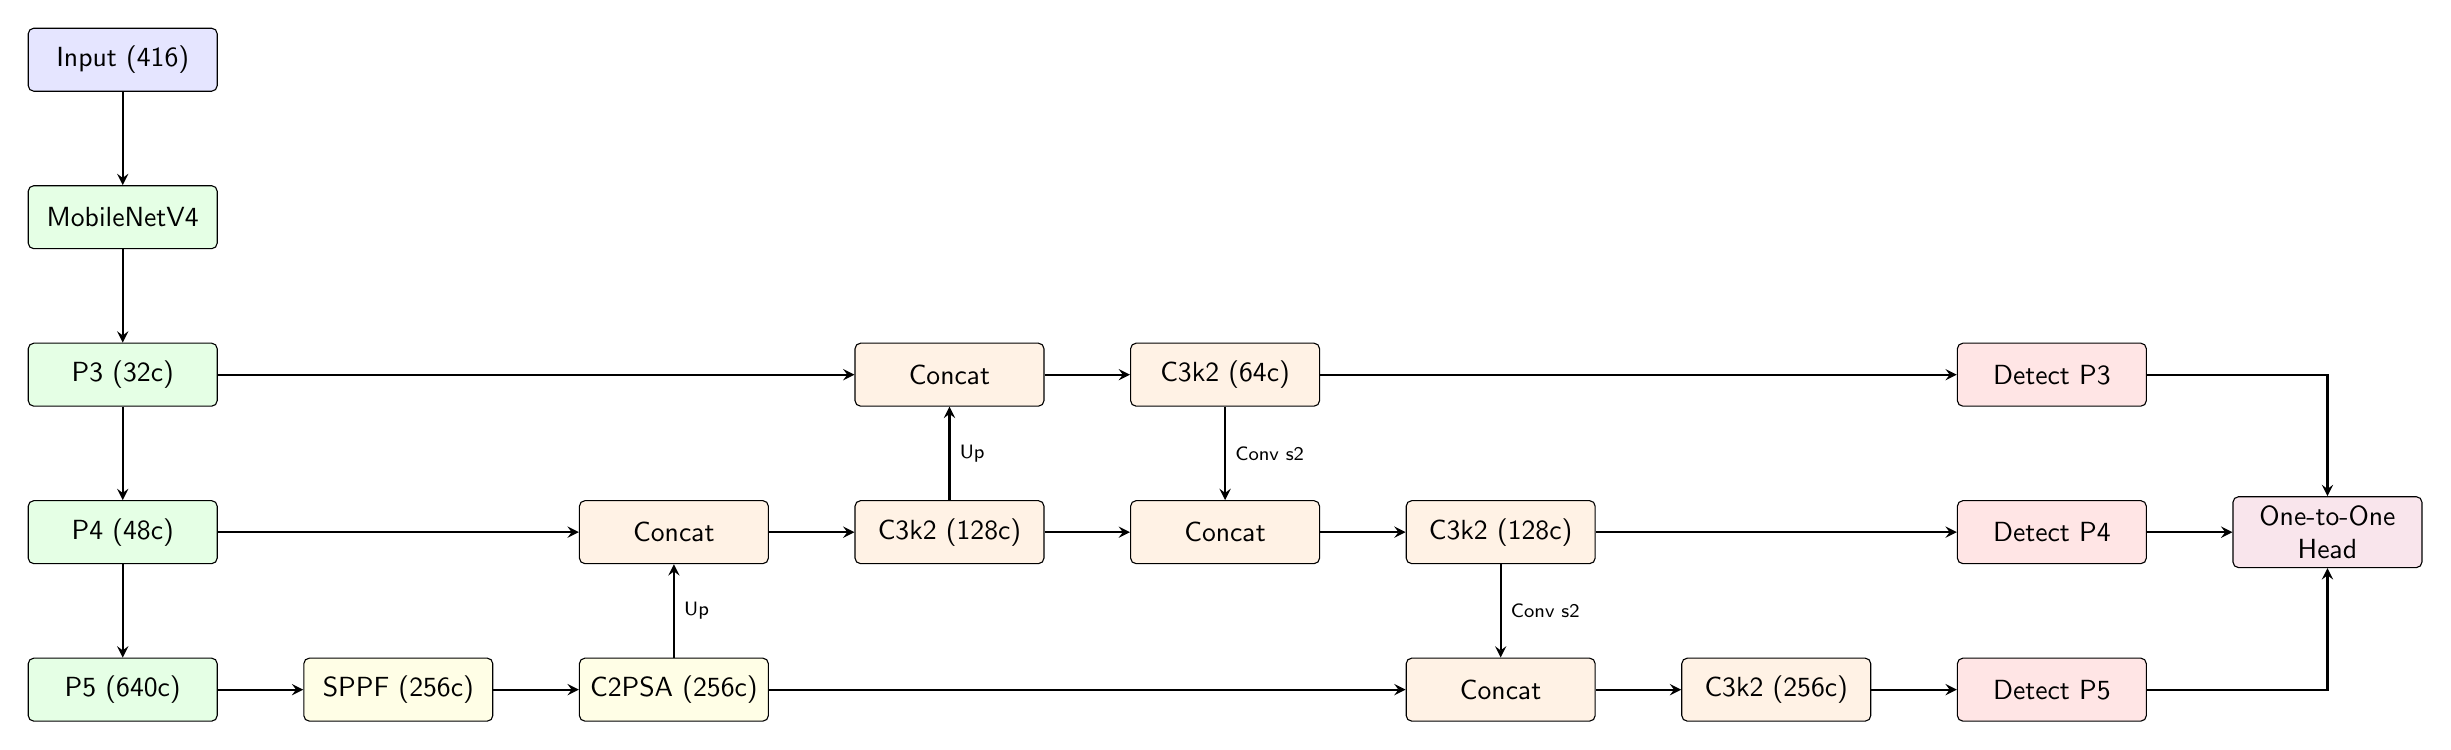
\begin{tikzpicture}[
        box/.style={rectangle, draw, minimum width=2.4cm, minimum height=0.8cm, text centered, font=\sffamily, rounded corners=2pt},
        arrow/.style={->, >=stealth, thick},
        label/.style={font=\sffamily\scriptsize}
    ]

    % X coordinates:
    % 0.0: Backbone
    % 3.5: SPPF
    % 7.0: C2PSA, cat1
    % 10.5: c3k2_1, cat2
    % 14.0: c3k2_2, cat3
    % 17.5: c3k2_3, cat4
    % 21.0: c3k2_4
    % 24.5: Detectors
    % 28.0: Head

    % Backbone
    \node[box, fill=blue!10] (input) at (0, 8) {Input (416)};
    \node[box, fill=green!10] (mnv4) at (0, 6) {MobileNetV4};
    \node[box, fill=green!10] (p3) at (0, 4) {P3 (32c)};
    \node[box, fill=green!10] (p4) at (0, 2) {P4 (48c)};
    \node[box, fill=green!10] (p5) at (0, 0) {P5 (640c)};

    \draw[arrow] (input) -- (mnv4);
    \draw[arrow] (mnv4) -- (p3);
    \draw[arrow] (p3) -- (p4);
    \draw[arrow] (p4) -- (p5);

    % SPPF & C2PSA
    \node[box, fill=yellow!10] (sppf) at (3.5, 0) {SPPF (256c)};
    \node[box, fill=yellow!10] (c2psa) at (7.0, 0) {C2PSA (256c)};
    \draw[arrow] (p5) -- (sppf);
    \draw[arrow] (sppf) -- (c2psa);

    % Neck - Top-down
    \node[box, fill=orange!10] (cat1) at (7.0, 2) {Concat};
    \node[box, fill=orange!10] (c3k2_1) at (10.5, 2) {C3k2 (128c)};
    \draw[arrow] (c2psa) -- node[right, label] {Up} (cat1);
    \draw[arrow] (p4) -- (cat1);
    \draw[arrow] (cat1) -- (c3k2_1);

    \node[box, fill=orange!10] (cat2) at (10.5, 4) {Concat};
    \node[box, fill=orange!10] (c3k2_2) at (14.0, 4) {C3k2 (64c)};
    \draw[arrow] (c3k2_1) -- node[right, label] {Up} (cat2);
    \draw[arrow] (p3) -- (cat2);
    \draw[arrow] (cat2) -- (c3k2_2);

    % Neck - Bottom-up
    \node[box, fill=orange!10] (cat3) at (14.0, 2) {Concat};
    \node[box, fill=orange!10] (c3k2_3) at (17.5, 2) {C3k2 (128c)};
    \draw[arrow] (c3k2_2) -- node[right, label] {Conv s2} (cat3);
    \draw[arrow] (c3k2_1) -- (cat3);
    \draw[arrow] (cat3) -- (c3k2_3);

    \node[box, fill=orange!10] (cat4) at (17.5, 0) {Concat};
    \node[box, fill=orange!10] (c3k2_4) at (21.0, 0) {C3k2 (256c)};
    \draw[arrow] (c3k2_3) -- node[right, label] {Conv s2} (cat4);
    \draw[arrow] (c2psa) -- (cat4);
    \draw[arrow] (cat4) -- (c3k2_4);

    % Detectors
    \node[box, fill=red!10] (head1) at (24.5, 4) {Detect P3};
    \node[box, fill=red!10] (head2) at (24.5, 2) {Detect P4};
    \node[box, fill=red!10] (head3) at (24.5, 0) {Detect P5};
    
    \node[box, fill=purple!10, align=center] (detect) at (28.0, 2) {One-to-One\\Head};

    \draw[arrow] (c3k2_2) -- (head1);
    \draw[arrow] (c3k2_3) -- (head2);
    \draw[arrow] (c3k2_4) -- (head3);
    
    \draw[arrow] (head1) -| (detect);
    \draw[arrow] (head2) -- (detect);
    \draw[arrow] (head3) -| (detect);

    \end{tikzpicture}
    }
    \vspace{0.5cm} % Add some space before caption to prevent overlap
    \caption{Architecture of the YOLO26 model with MobileNetV4ConvSmall050 backbone, dual-head mechanism, and NMS-free end-to-end detection, tailored for $416\times416$ resolution.}
    \label{fig:yolo26_mnv4_arch}
\end{figure}

% \subsection{Training Hyperparameters}

% The training process is conducted using the Ultralytics YOLO training API, which provides a reproducible and configurable pipeline for object detection tasks. The dataset is specified through a YAML configuration file (\texttt{TrafficLightV5.v9i.yolo26/data.yaml}) that defines training and validation image paths, class labels, and metadata. To bootstrap training, pretrained weights from \texttt{yolo26n.pt} are loaded via partial weight transfer; compatible layers (primarily in the neck and head) inherit learned parameters, while the MobileNetV4 backbone is initialised from scratch. The \texttt{end2end=True} flag activates the One-to-One head for NMS-free training. Table~\ref{tab:hyperparams} summarises the key hyperparameters.

% \begin{table}[htbp]
% \centering
% \caption{Selected training hyperparameters for the YOLO26-MobileNetV4 model.}
% \label{tab:hyperparams}
% \renewcommand{\arraystretch}{1.15}
% \begin{tabular}{l l l}
% \hline
% \textbf{Parameter} & \textbf{Value} & \textbf{Rationale} \\
% \hline
% \texttt{imgsz} & $416 \times 416$ & Balance between spatial resolution and edge inference speed \\
% \texttt{epochs} & 100 & Sufficient convergence for the modified backbone \\
% \texttt{batch} & 16 & Fits within GPU memory with MobileNetV4 backbone \\
% \texttt{patience} & 100 & Disable early stopping; run full cosine LR cycle \\
% \texttt{optimizer} & auto (SGD) & Stable convergence for detection models \\
% \texttt{lr0} & 0.005 & Slightly elevated initial LR for unfrozen backbone \\
% \texttt{lrf} & 0.01 & Final LR ratio: $\text{lr}_{\text{final}} = 0.01 \times \text{lr}_0$ \\
% \texttt{cos\_lr} & True & Cosine annealing for smooth convergence in late epochs \\
% \texttt{warmup\_epochs} & 3.0 & Gradual LR ramp-up to stabilise early gradients \\
% \texttt{amp} & True & Mixed-precision training for memory efficiency \\
% \texttt{freeze} & None & All layers trainable; no backbone freezing \\
% \texttt{close\_mosaic} & 10 & Disable mosaic augmentation in the last 10 epochs \\
% \hline
% \texttt{box} & 7.5 & Bounding box regression loss weight \\
% \texttt{cls} & 0.5 & Classification loss weight \\
% \texttt{dfl} & 1.5 & DFL loss weight (set but unused since YOLO26 removes DFL) \\
% \hline
% \end{tabular}
% \end{table}

% \subsubsection{Optimiser and Learning Rate Schedule}
% The optimiser is set to \texttt{auto}, which defaults to Stochastic Gradient Descent (SGD) with Nesterov momentum ($\mu = 0.937$) and weight decay ($\lambda = 5 \times 10^{-4}$). The initial learning rate is set to $\text{lr}_0 = 0.005$, slightly higher than the default $0.01$ to compensate for the unfrozen MobileNetV4 backbone requiring larger gradient steps to adapt to the traffic light domain. A cosine annealing schedule (\texttt{cos\_lr=True}) smoothly decays the learning rate to $\text{lr}_0 \times \text{lrf} = 5 \times 10^{-5}$ over the full 100 epochs, ensuring fine-grained convergence in the later stages of training without the abrupt transitions of step-decay schedules.

% \subsubsection{No Backbone Freezing}
% Unlike transfer learning approaches that freeze the backbone during initial epochs, this configuration leaves all layers trainable (\texttt{freeze=None}). Since the MobileNetV4ConvSmall050 backbone differs fundamentally from the original YOLO26 backbone, the pretrained weights only partially transfer. Freezing would prevent the new backbone from learning domain-specific features such as the distinctive shapes and colours of Vietnamese traffic light signal heads and arrow indicators.

% \subsubsection{Image Augmentation Strategy}
% The augmentation pipeline is carefully tuned for the traffic light detection domain:

% \begin{itemize}
%     \item \textbf{Colour jitter}: Hue shift is minimal (\texttt{hsv\_h}$=0.015$) to preserve the critical red/green/yellow colour semantics of traffic signals. Saturation (\texttt{hsv\_s}$=0.7$) and brightness (\texttt{hsv\_v}$=0.4$) augmentation are moderate to improve robustness under varying lighting conditions without corrupting colour-dependent class distinctions.
%     \item \textbf{Geometric transforms}: Translation (\texttt{translate}$=0.1$) and scale (\texttt{scale}$=0.5$) are enabled to simulate varying camera distances and positions. Rotation (\texttt{degrees}$=0.0$) and shear (\texttt{shear}$=0.0$) are disabled since traffic lights are always vertically oriented.
%     \item \textbf{Flipping disabled}: Both horizontal (\texttt{fliplr}$=0.0$) and vertical (\texttt{flipud}$=0.0$) flips are strictly disabled. Horizontal flipping would reverse the direction of left/right arrow turn signals, creating incorrect training labels.
%     \item \textbf{Mosaic}: Set to 0.5 probability to composite multiple training images into one frame, improving the model's ability to detect small, densely packed objects such as timer digit clusters. Mosaic is automatically disabled in the last 10 epochs (\texttt{close\_mosaic}$=10$) so the model fine-tunes on unmodified real images.
%     \item \textbf{MixUp and CopyPaste}: Both disabled (\texttt{mixup}$=0.0$, \texttt{copy\_paste}$=0.0$) to avoid blending signals from different classes, which could confuse the network on colour-critical traffic light states.
% \end{itemize}


\subsection{Dataset and Hyper parameters}
\label{sub:datasetYolo}
A well-prepared dataset and carefully tuned hyperparameters are essential for successfully training the modified YOLO-MobileNetV4 model. This section details the dataset used for traffic light detection, including its composition and pre-processing steps, before explaining the specific training configurations and augmentation strategies applied to ensure robust performance.

\subsubsection{Dataset Composition and Pre-processing}
The model is trained and evaluated on the \texttt{TrafficLightV5.v9i.yolo26} dataset, which comprises a total of 4,867 images. The dataset is annotated in the YOLO format and structured to detect four classes: \texttt{left}, \texttt{right}, \texttt{straight}, and \texttt{timer}. The images are partitioned into three splits: 4,260 images for training, 406 for validation, and 201 for testing. Prior to model ingestion, offline pre-processing and augmentations were applied via Roboflow. The pre-processing includes auto-orientation and resizing to $416 \times 416$ pixels (fit with black edges). The offline augmentation strategy generates three versions of each source image by applying random rotation ($-5^\circ$ to $+5^\circ$), random shear ($-2^\circ$ to $+2^\circ$), exposure adjustments ($\pm 10\%$), and salt-and-pepper noise ($0.1\%$ of pixels).

\subsubsection{Training Configuration}
The training process is conducted using the Ultralytics YOLO training API, which provides a reproducible and configurable pipeline for object detection tasks. The dataset is specified through a YAML configuration file (\texttt{TrafficLightV5.v9i.yolo26/data.yaml}) that defines training and validation image paths, class labels, and metadata. To bootstrap training, pretrained weights from \texttt{yolo26n.pt} are loaded via partial weight transfer; compatible layers (primarily in the neck and head) inherit learned parameters, while the MobileNetV4 backbone is initialised from scratch. The \texttt{end2end=True} flag activates the One-to-One head for NMS-free training. Table~\ref{tab:hyperparams} summarises the key hyperparameters.

\begin{table}[htbp]
\centering
\caption{Selected training hyperparameters for the YOLO26-MobileNetV4 model.}
\label{tab:hyperparams}
\renewcommand{\arraystretch}{1.15}
\begin{tabular}{l l l}
\hline
\textbf{Parameter} & \textbf{Value} & \textbf{Rationale} \\
\hline
\texttt{imgsz} & $416 \times 416$ & Balance between spatial resolution and edge inference speed \\
\texttt{epochs} & 100 & Sufficient convergence for the modified backbone \\
\texttt{batch} & 16 & Fits within GPU memory with MobileNetV4 backbone \\
\texttt{patience} & 100 & Disable early stopping; run full cosine LR cycle \\
\texttt{optimizer} & auto (SGD) & Stable convergence for detection models \\
\texttt{lr0} & 0.005 & Slightly elevated initial LR for unfrozen backbone \\
\texttt{lrf} & 0.01 & Final LR ratio: $\text{lr}_{\text{final}} = 0.01 \times \text{lr}_0$ \\
\texttt{cos\_lr} & True & Cosine annealing for smooth convergence in late epochs \\
\texttt{warmup\_epochs} & 3.0 & Gradual LR ramp-up to stabilise early gradients \\
\texttt{amp} & True & Mixed-precision training for memory efficiency \\
\texttt{freeze} & None & All layers trainable; no backbone freezing \\
\texttt{close\_mosaic} & 10 & Disable mosaic augmentation in the last 10 epochs \\
\hline
\texttt{box} & 7.5 & Bounding box regression loss weight \\
\texttt{cls} & 0.5 & Classification loss weight \\
\texttt{dfl} & 1.5 & DFL loss weight (set but unused since YOLO26 removes DFL) \\
\hline
\end{tabular}
\end{table}

\subsubsection{Optimiser and Learning Rate Schedule}
The optimiser is set to \texttt{auto}, which defaults to Stochastic Gradient Descent (SGD) with Nesterov momentum ($\mu = 0.937$) and weight decay ($\lambda = 5 \times 10^{-4}$). The initial learning rate is set to $\text{lr}_0 = 0.005$, slightly higher than the default $0.01$ to compensate for the unfrozen MobileNetV4 backbone requiring larger gradient steps to adapt to the traffic light domain. A cosine annealing schedule (\texttt{cos\_lr=True}) smoothly decays the learning rate to $\text{lr}_0 \times \text{lrf} = 5 \times 10^{-5}$ over the full 100 epochs, ensuring fine-grained convergence in the later stages of training without the abrupt transitions of step-decay schedules.

\subsubsection{No Backbone Freezing}
Unlike transfer learning approaches that freeze the backbone during initial epochs, this configuration leaves all layers trainable (\texttt{freeze=None}). Since the MobileNetV4ConvSmall050 backbone differs fundamentally from the original YOLO26 backbone, the pretrained weights only partially transfer. Freezing would prevent the new backbone from learning domain-specific features such as the distinctive shapes and colours of Vietnamese traffic light signal heads and arrow indicators.

\subsubsection{Image Augmentation Strategy}
The augmentation pipeline is carefully tuned for the traffic light detection domain:

\begin{itemize}
    \item \textbf{Colour jitter}: Hue shift is minimal (\texttt{hsv\_h}$=0.015$) to preserve the critical red/green/yellow colour semantics of traffic signals. Saturation (\texttt{hsv\_s}$=0.7$) and brightness (\texttt{hsv\_v}$=0.4$) augmentation are moderate to improve robustness under varying lighting conditions without corrupting colour-dependent class distinctions.
    \item \textbf{Geometric transforms}: Translation (\texttt{translate}$=0.1$) and scale (\texttt{scale}$=0.5$) are enabled to simulate varying camera distances and positions. Rotation (\texttt{degrees}$=0.0$) and shear (\texttt{shear}$=0.0$) are disabled since traffic lights are always vertically oriented.
    \item \textbf{Flipping disabled}: Both horizontal (\texttt{fliplr}$=0.0$) and vertical (\texttt{flipud}$=0.0$) flips are strictly disabled. Horizontal flipping would reverse the direction of left/right arrow turn signals, creating incorrect training labels.
    \item \textbf{Mosaic}: Set to 0.5 probability to composite multiple training images into one frame, improving the model's ability to detect small, densely packed objects such as timer digit clusters. Mosaic is automatically disabled in the last 10 epochs (\texttt{close\_mosaic}$=10$) so the model fine-tunes on unmodified real images.
    \item \textbf{MixUp and CopyPaste}: Both disabled (\texttt{mixup}$=0.0$, \texttt{copy\_paste}$=0.0$) to avoid blending signals from different classes, which could confuse the network on colour-critical traffic light states.
\end{itemize}

\subsection{Exporting to TFLite with INT8 Quantisation}

To deploy the trained YOLO26-MobileNetV4 model on edge devices such as the Raspberry Pi 5, the model must be converted from its native PyTorch format to TensorFlow Lite (TFLite). The Ultralytics export pipeline automates this multi-stage conversion: PyTorch $\to$ ONNX $\to$ TensorFlow SavedModel $\to$ TFLite. The export is performed with the following configuration:

\begin{lstlisting}[language=Python, caption={YOLO26-MobileNetV4 TFLite export script.}, label={lst:export}]
from ultralytics import YOLO

model = YOLO("runs/train/yolo26_mobilenetv4_custom/weights/best.pt")

model.export(
    format="tflite",
    imgsz=416,
    int8=True,
    data='TrafficLightV5.v9i.yolo26/data.yaml',
    batch=1,
    end2end=True,
)
\end{lstlisting}

\subsubsection{INT8 Post-Training Quantisation.}
Full-integer quantisation maps all floating-point weights and activations to 8-bit integers, reducing the model size by approximately $4\times$ and enabling the use of integer-only arithmetic on ARM NEON SIMD units. The quantisation scheme represents each tensor value $x$ as:

\begin{equation}
\label{eq:quant}
  x_q = \text{round}\!\left(\frac{x}{s}\right) + z,
  \qquad
  s = \frac{x_{\max} - x_{\min}}{255},
  \qquad
  z = \text{round}\!\left(-\frac{x_{\min}}{s}\right),
\end{equation}

where $s$ is the per-tensor scale factor and $z$ is the zero-point, both determined during the calibration phase. To compute these statistics, a representative subset of training images from the dataset specified by the \texttt{data} parameter is fed through the network. This calibration step records the dynamic range of each activation tensor, enabling the converter to choose optimal scale and zero-point values that minimise quantisation error across the domain-specific input distribution.

\subsubsection{End-to-End Export}
The \texttt{end2end=True} flag preserves the One-to-One detection head in the exported model graph, ensuring that the TFLite model produces final detection results directly without requiring an external NMS post-processing step. This is critical for edge deployment because it eliminates the need for custom NMS operators that may not be supported by all TFLite delegates, and guarantees deterministic output tensor shapes $(1, 300, 6)$ regardless of input content.

\subsubsection{Deployment Considerations}
The resulting INT8 TFLite model is deployed via the LiteRT (formerly TensorFlow Lite) interpreter on the target device. With \texttt{batch=1} and \texttt{imgsz=416}, the model is optimised for single-frame, real-time inference. The quantised flatbuffer file is significantly smaller than the original float32 model, fitting within the L2 cache of the Cortex-A76 cores on the Raspberry Pi 5, which minimises memory access latency during inference.

% \subsubsection{Accuracy}

% Based on the quantitative trends observed in Figures~\ref{fig:yolomobilenetv4} and~\ref{fig:code_generation}, the original YOLOv11n model achieves slightly higher detection accuracy compared to the YOLOv11n-MobileNetV4 variant. Specifically, the original model attains marginally better precision, recall, and mean Average Precision across the evaluated metrics.

% From the mAP@50 curves, the original YOLOv11n model achieves an improvement of approximately 10--15\% compared to the MobileNetV4-based model. A similar performance gap is observed for mAP@50--95, where the original architecture demonstrates around 10--15\% higher accuracy under stricter localization thresholds. These differences indicate that the original backbone provides stronger feature representation capability, particularly for precise object localization.

% Nevertheless, the overall performance gap remains relatively small. The YOLO-MobileNetV4 model preserves more than 95\% of the detection accuracy achieved by the original YOLOv11n while significantly reducing model complexity. Precision and recall curves further confirm that both models exhibit comparable convergence behavior, with the MobileNetV4 variant showing slightly lower but stable accuracy throughout training.

% These results highlight a clear trade off between accuracy and efficiency. While the original YOLOv11n model offers slightly superior detection accuracy, the YOLO-MobileNetV4 configuration provides a more balanced solution by achieving competitive accuracy with reduced computational cost. This balance makes the MobileNetV4-based model particularly suitable for deployment in edge oriented and resource constrained environments where efficiency is a primary concern.


% \begin{figure}[H]
%     \centering
%     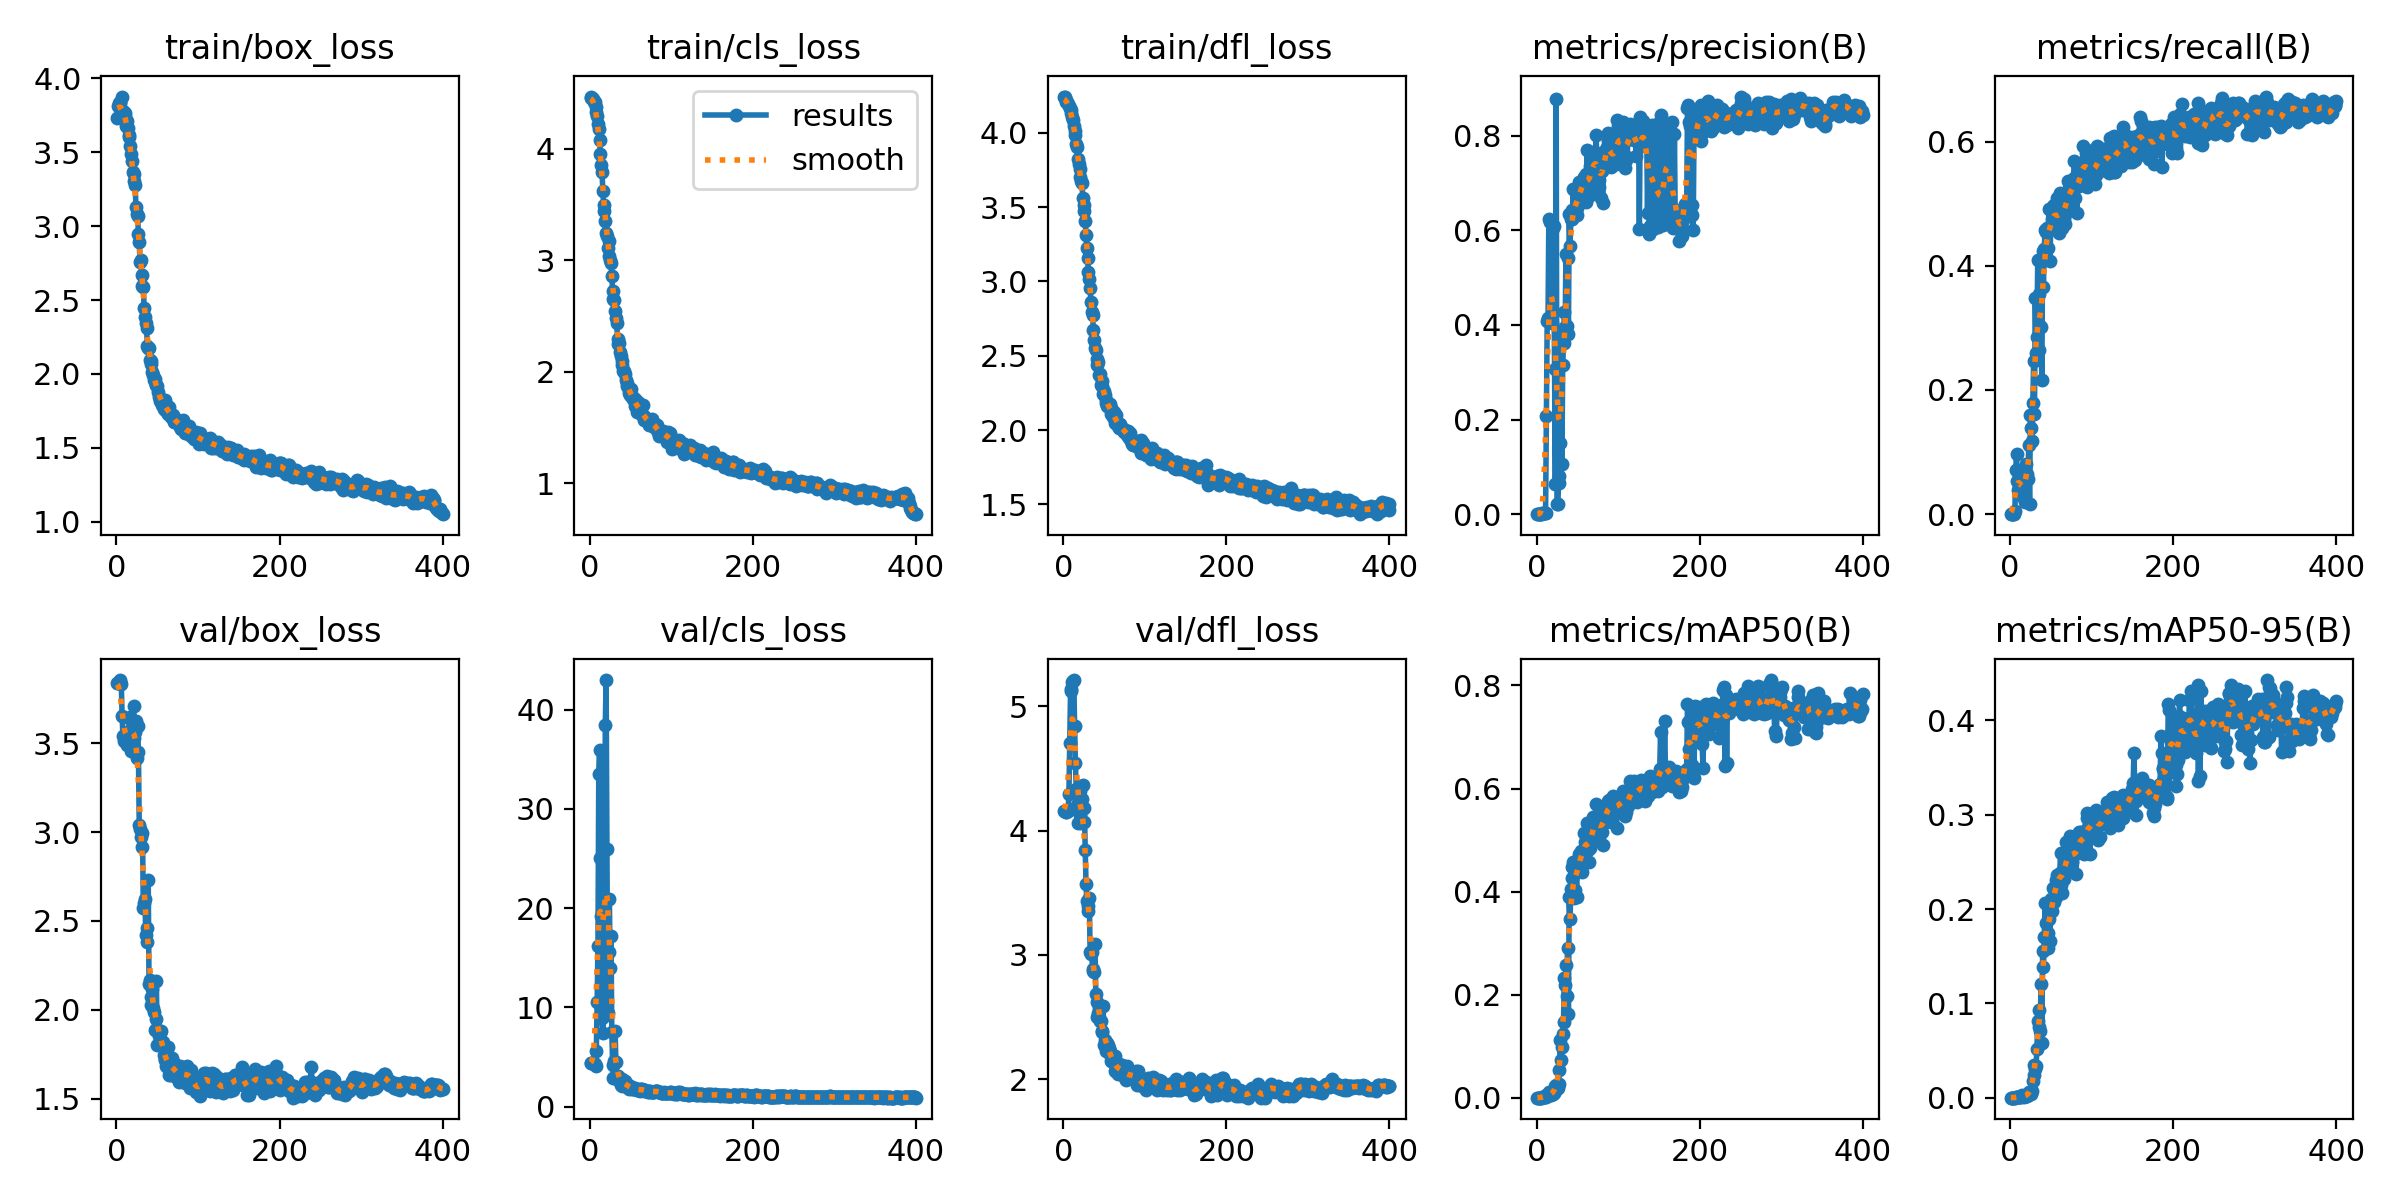
\includegraphics[width=0.75\textwidth]{Images/chap3/yolo/yolomobilenetv4.png}
%     \vspace{0.5cm}
%     \caption{The accuracy of Yolov11n-MobileNetV4}
%     \label{fig:yolomobilenetv4}
% \end{figure}

% \begin{figure}[H]
%     \centering
%     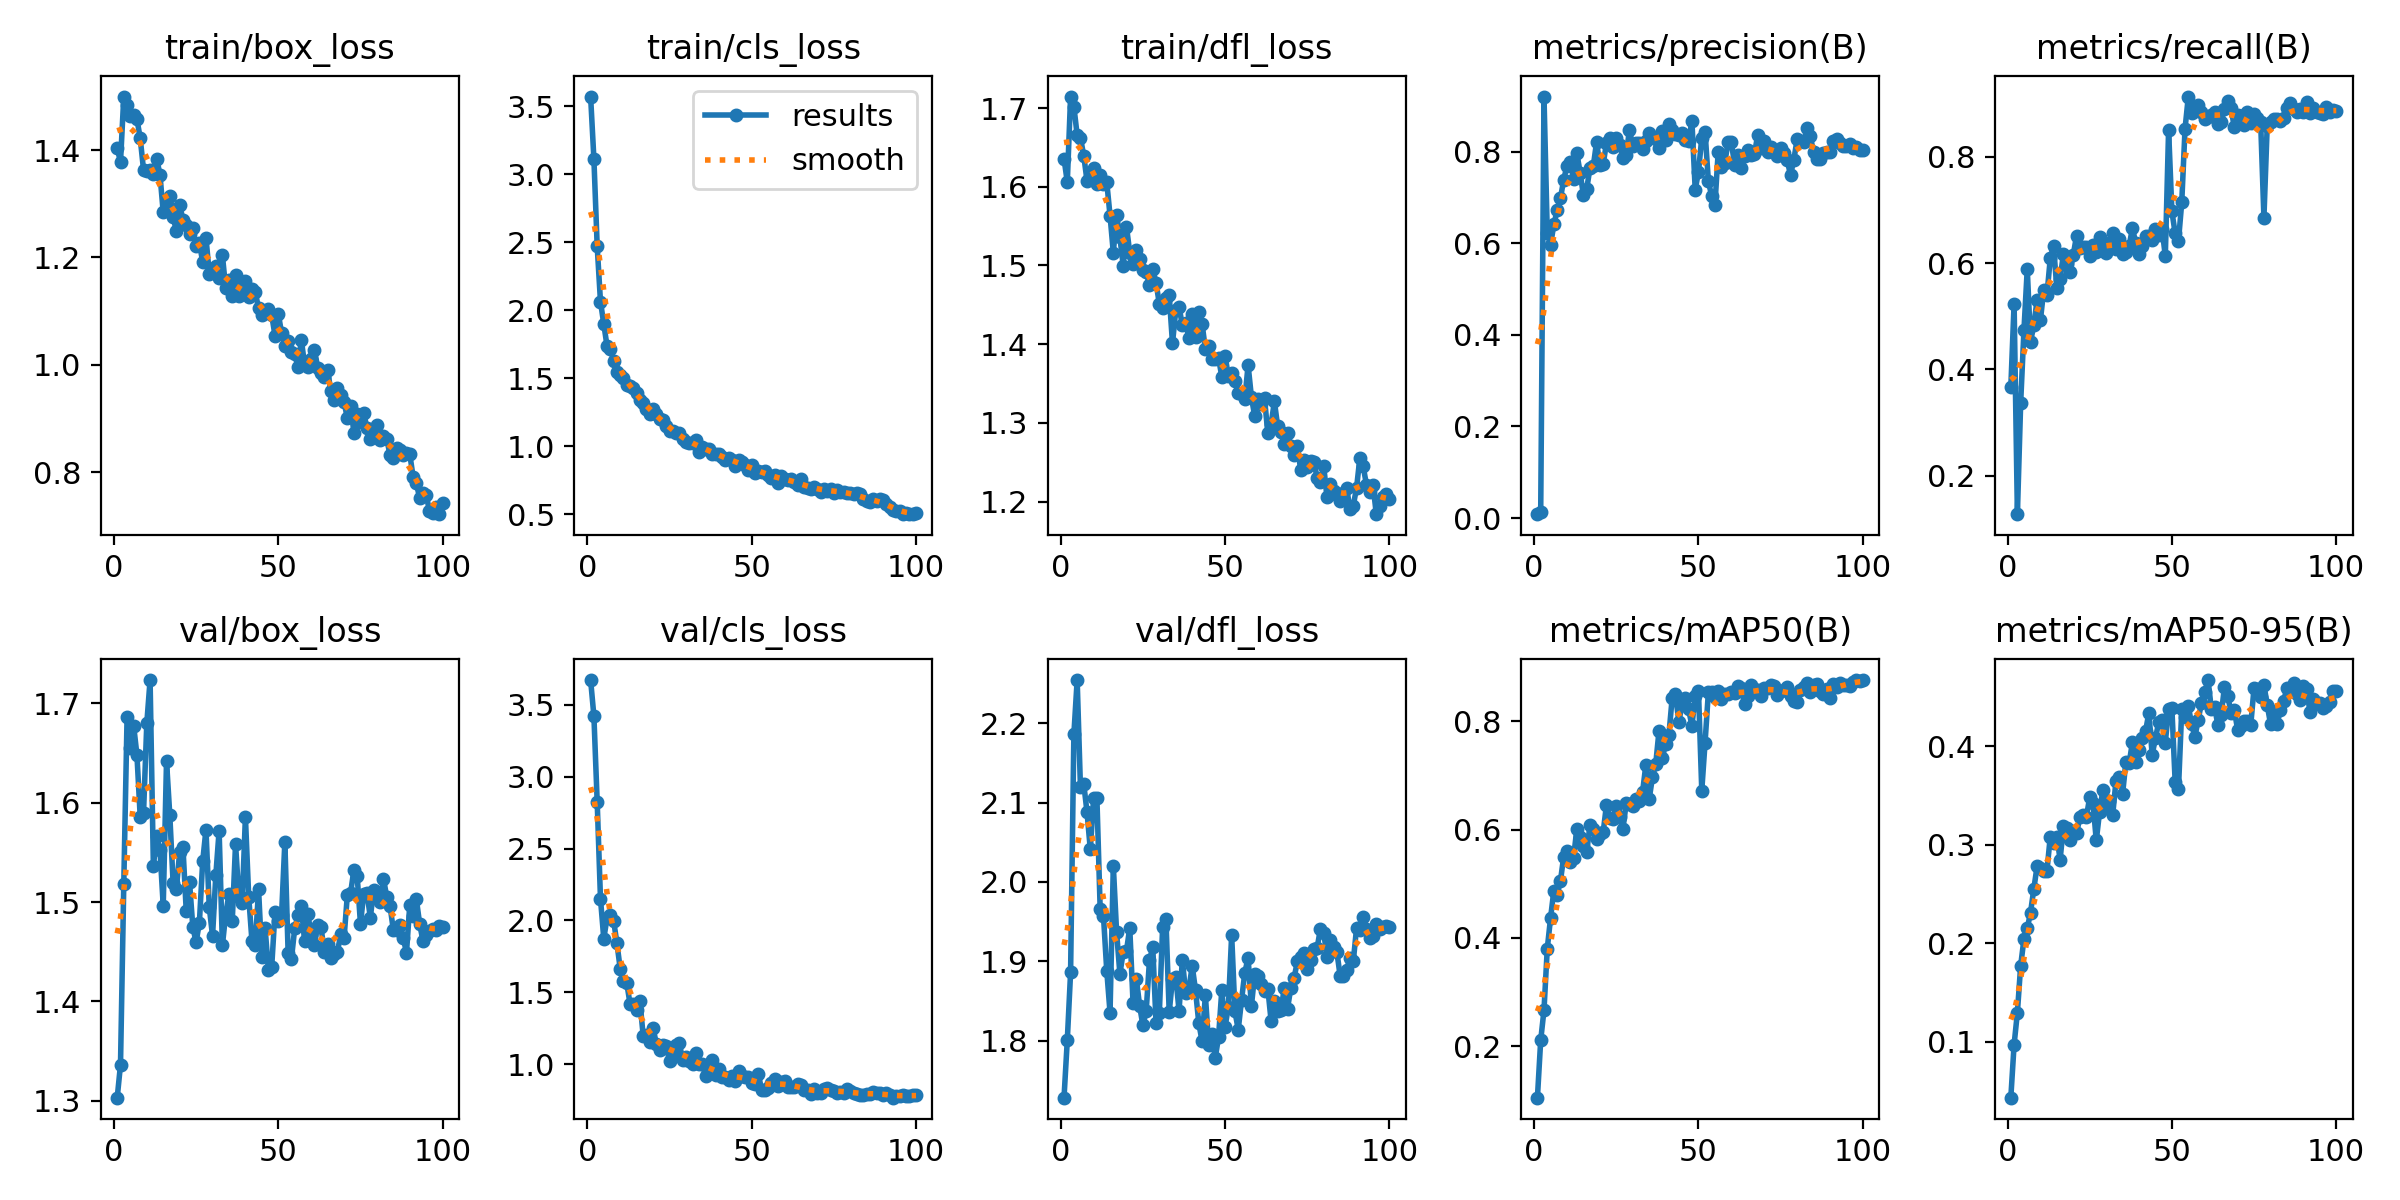
\includegraphics[width=0.75\textwidth]{Images/chap3/yolo/original.png}
%     \vspace{0.5cm}
%     \caption{The accuracy of original Yolov11n}
%     \label{fig:yolo11n}
% \end{figure}

% \subsubsection{Inference Speed}

% Inference speed is a key requirement for real time deployment on resource constrained platforms such as Raspberry Pi. According to the official Ultralytics benchmark, the original YOLO model converted to TensorFlow Lite requires more than 400\,ms per inference on Raspberry Pi class hardware when executed on CPU\footnote{Detailed benchmarking results for YOLO models on Raspberry Pi are reported by Ultralytics at \url{https://docs.ultralytics.com/vi/guides/raspberry-pi/\#detailed-comparison-table}.}. This latency corresponds to a processing rate of approximately 2--3 frames per second, which is insufficient for real time applications.

% In contrast, experimental results obtained in this work show that the YOLO-MobileNetV4 model achieves an average inference time of 30--40\,ms per frame after conversion to the TFLite format. This corresponds to an effective processing speed of approximately 25--33 frames per second. Compared to the original YOLO TFLite model, the MobileNetV4 based configuration reduces inference latency by approximately 360--370\,ms per frame.

% In relative terms, this represents a speed improvement of about 10--13 times. Equivalently, the inference time is reduced by approximately 90--92\% compared to the original YOLO TFLite implementation. Such a significant reduction enables near real time performance on CPU only embedded devices.

% The observed speedup is primarily attributed to the lightweight architecture of the MobileNetV4 backbone, which substantially reduces the number of parameters and floating point operations. As a result, the YOLO-MobileNetV4 model achieves a much more favorable balance between detection accuracy and inference speed, making it well suited for real time edge deployment on Raspberry Pi platforms.

% \begin{figure}[H]
%     \centering
%     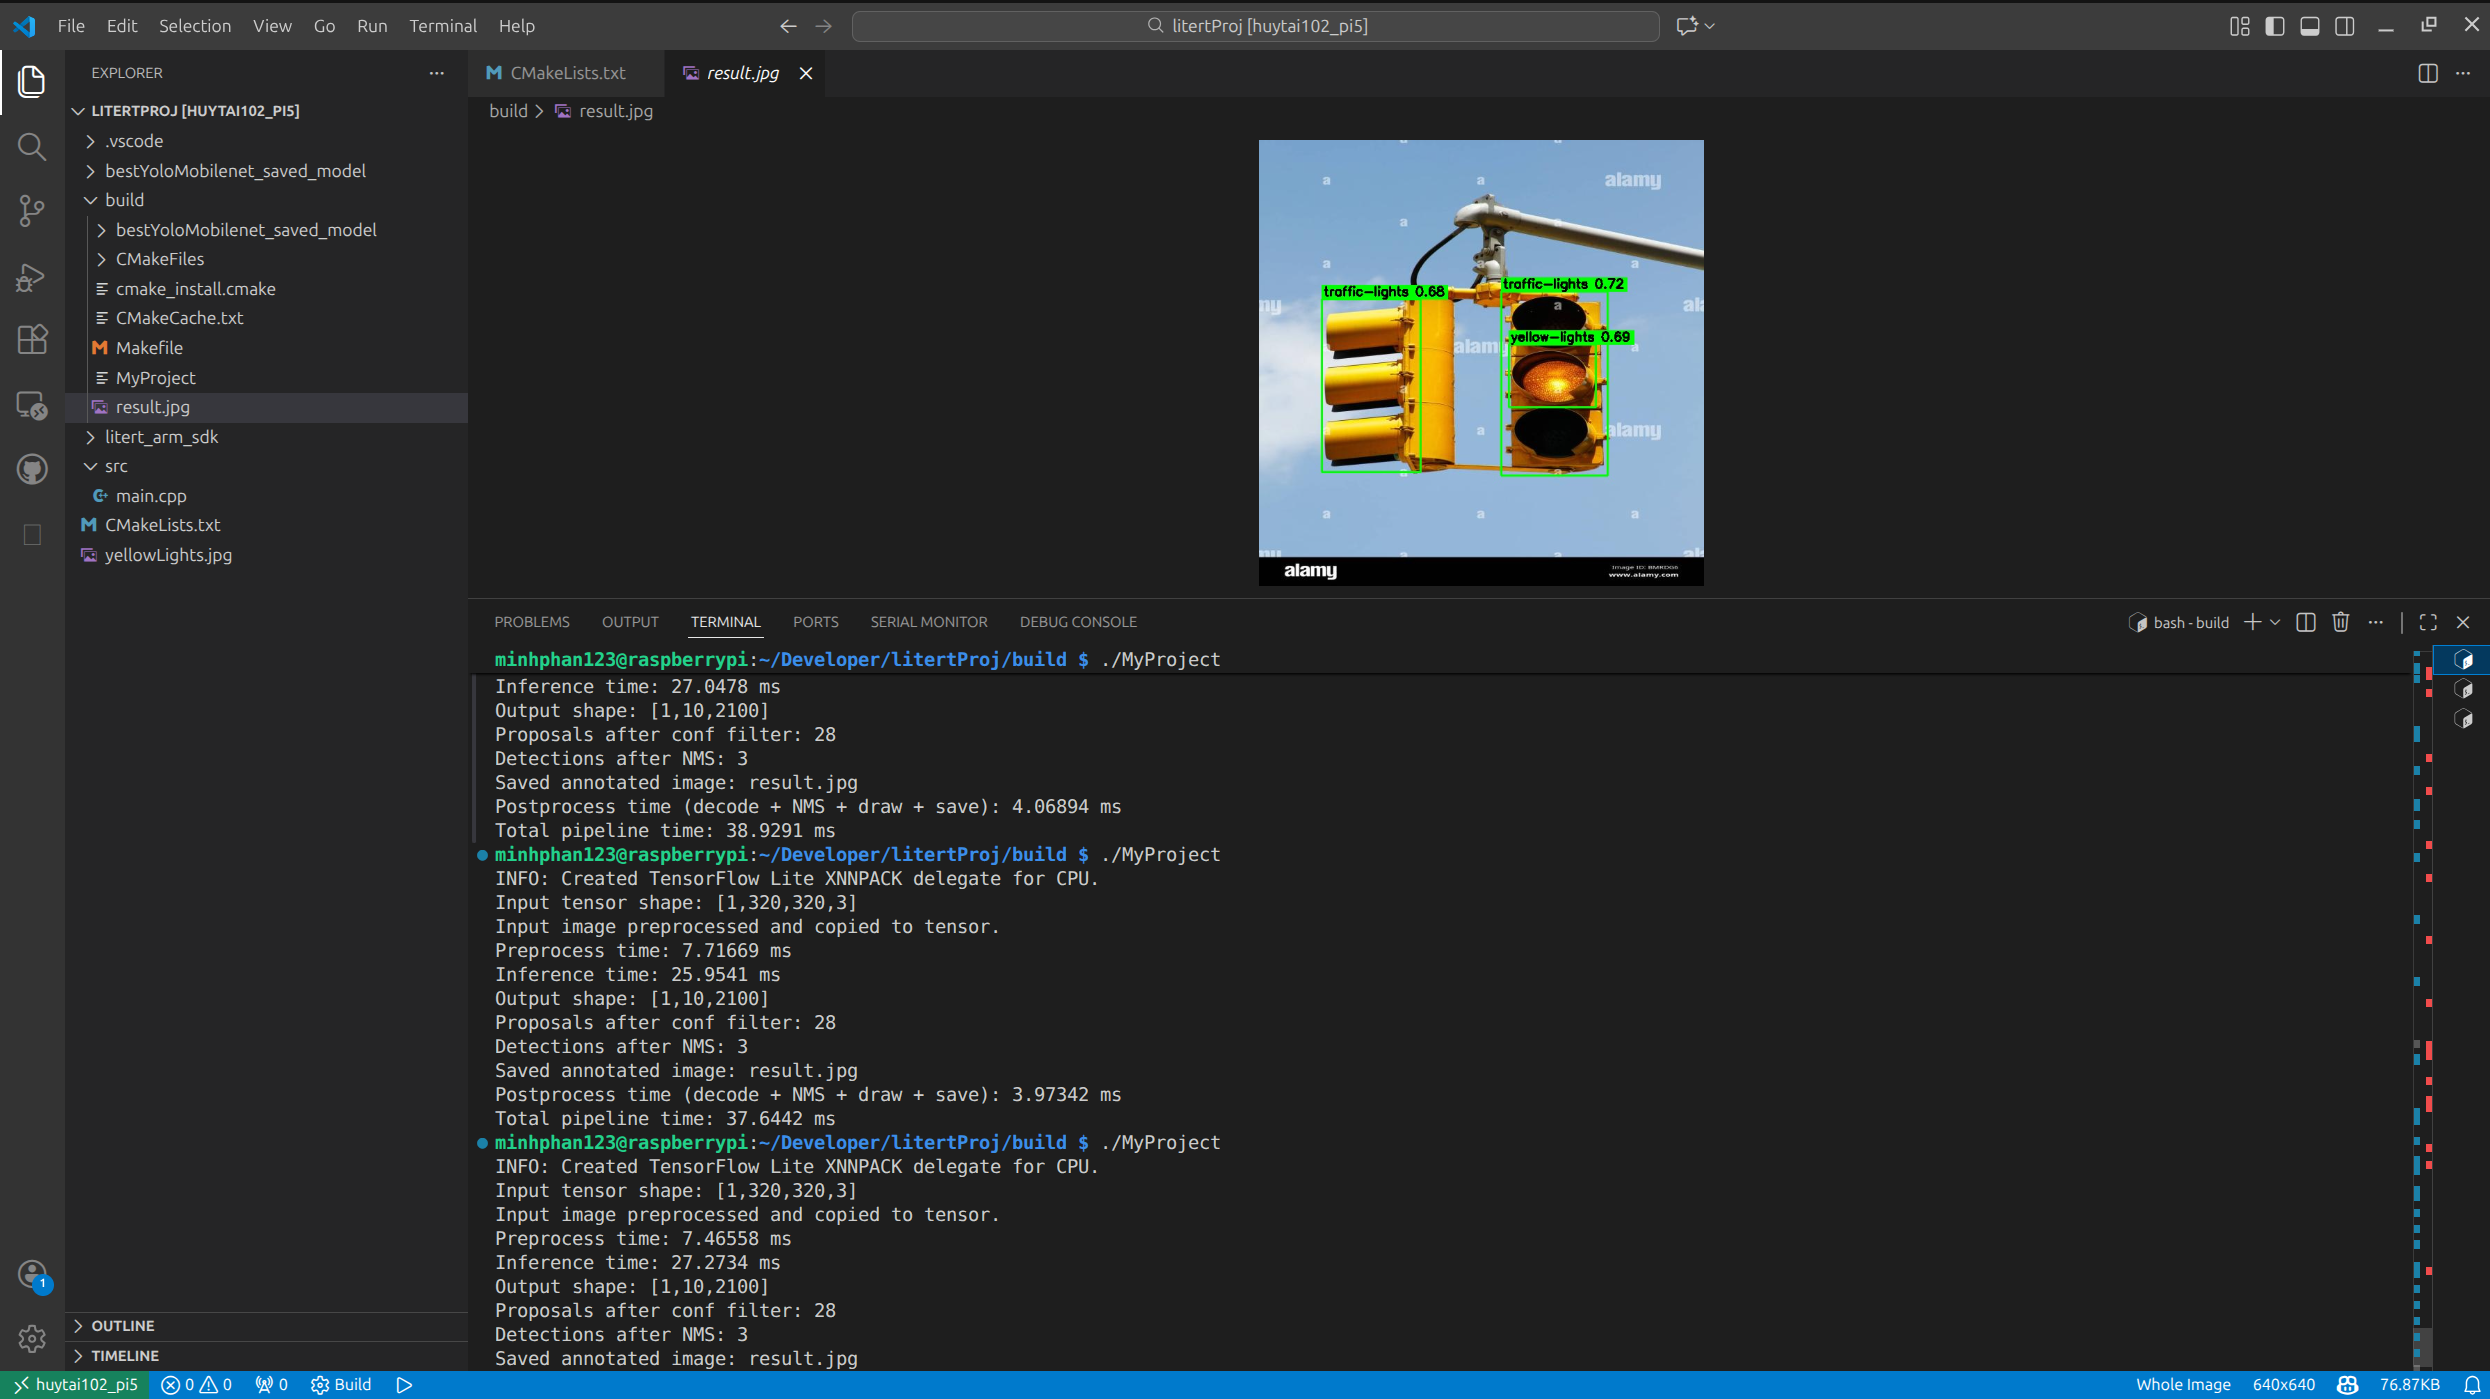
\includegraphics[width=0.75\textwidth]{Images/chap3/yolo/inference_speed.png}
%     \vspace{0.5cm}
%     \caption{The inference time of Yolovv11n-MobileNetV4 model}
%     \label{fig:infer_time_yolo11n_mobilenetv4}
% \end{figure}


% \begin{table}[H]
% \centering
% \label{tab:tradeoff_yolo_models}
% \begin{tabular}{|l|c|c|}
% \hline
% \textbf{Metric} & \textbf{YOLOv11n (Original)} & \textbf{YOLOv11n-MobileNetV4} \\
% \hline
% Backbone & CSP-based YOLO backbone & MobileNetV4 (lightweight) \\
% \hline
% mAP@50 & Higher ($\approx$ +10--15\%) & Slightly lower \\
% \hline
% mAP@50--95 & Higher ($\approx$ +10--15\%) & Slightly lower \\
% \hline
% Precision / Recall & Marginally higher & Comparable and stable \\
% \hline
% Inference time (TFLite, CPU) & $>$400 ms & 30--40 ms \\
% \hline
% Throughput (FPS) & 2--3 FPS & 25--33 FPS \\
% \hline
% Speedup factor & 1$\times$ (baseline) & $\approx$10--13$\times$ faster \\
% \hline
% Inference time reduction & -- & $\approx$90--92\% \\
% \hline
% Model complexity & Higher & Significantly reduced \\
% \hline
% Suitability for edge deployment & Limited & Highly suitable \\
% \hline
% \textbf{Overall trade-off} & Higher accuracy & Better accuracy--speed balance \\
% \hline
% \end{tabular}
% \caption{Trade-off comparison between YOLOv11n and YOLOv11n-MobileNetV4}
% \end{table}

\subsection{Evaluation between Models}

To validate the architectural modifications introduced by the MobileNetV4 backbone replacement, a systematic benchmark was conducted comparing the original YOLO26n model against the proposed YOLO26n-MobileNetV4 variant. 

Both models were evaluated on the same TrafficLightV5 validation set under identical conditions: $416 \times 416$ input resolution, INT8 TFLite quantisation, batch size of 1, and end-to-end (NMS-free) inference mode. Table~\ref{tab:model_eval} summarises the results across latency and accuracy metrics.

\begin{table}[htbp]
\centering
\caption{Performance and accuracy comparison: YOLO26n Original vs.\ YOLO26n-MobileNetV4. Negative values in the change column indicate reduction (improvement for latency metrics; degradation for accuracy metrics). Asterisks (*) denote metrics where a decrease is an expected trade-off.}
\label{tab:model_eval}
\renewcommand{\arraystretch}{1.20}
\begin{tabular}{l r r r}
\hline
\textbf{Metric} & \textbf{YOLO26n Original} & \textbf{YOLO26n-MNv4} & \textbf{Change (\%)} \\
\hline
Samples processed           & 1\,074        & \textbf{1\,366}        & $+27.19$  \\
Avg.\ latency (Pi 5)        & 55.09\,ms     & \textbf{43.23\,ms}     & $-21.52$  \\
Max spike latency (Pi 5)    & 159.73\,ms    & \textbf{78.64\,ms}     & $-50.77$  \\
Min latency (Pi 5)          & 50.12\,ms     & \textbf{36.50\,ms}     & $-27.16$  \\
CPU inference (Intel)       & 15.21\,ms     & \textbf{12.33\,ms}     & $-18.93$  \\
mAP50                       & \textbf{89.90\%}       & 85.75\%       & $-4.15$\textsuperscript{*}  \\
mAP50--95                   & \textbf{56.61\% }      & 53.31\%       & $-3.30$\textsuperscript{*}  \\
\hline
\end{tabular}
\end{table}

\subsubsection{Latency Analysis}

The MobileNetV4 backbone delivers a substantial improvement across all latency metrics on the Raspberry Pi 5. The average per-frame inference time drops from 55.09\,ms to 43.23\,ms, a \textbf{21.52\% reduction} that raises the effective throughput from approximately 18\,FPS to 23\,FPS. More critically for safety-critical ADAS applications, the worst-case latency spike is reduced by \textbf{50.77\%} --- from 159.73\,ms to 78.64\,ms. Latency spikes exceeding 100\,ms are particularly hazardous in real-time perception loops because they can cause the planning module to operate on stale state estimates. The MobileNetV4 variant eliminates spikes above 80\,ms entirely, ensuring that even under worst-case conditions (thermal throttling, OS scheduling jitter), the perception system delivers updates within the 67\,ms budget required for 15\,FPS operation.

The minimum latency (best-case scenario) also improves from 50.12\,ms to 36.50\,ms ($-27.16\%$), confirming that the speed gain is architectural rather than an artefact of measurement variance. On the Intel development CPU, inference time decreases from 15.21\,ms to 12.33\,ms ($-18.93\%$), demonstrating that MobileNetV4's universal efficiency extends beyond ARM to x86 hardware as well.

\subsubsection{Accuracy Analysis}

The accuracy metrics show a moderate decrease: mAP50 drops from 89.90\% to 85.75\% ($-4.15$ percentage points), and mAP50--95 drops from 56.61\% to 53.31\% ($-3.30$ percentage points). This reduction is expected and acceptable for several reasons:

\begin{enumerate}
    \item \textbf{Backbone capacity reduction}: The MobileNetV4ConvSmall050 backbone has significantly fewer parameters and FLOPs than the original YOLO26 CSP-based backbone. The 050 suffix indicates a 50\% width multiplier, which halves all channel dimensions relative to the full MobileNetV4ConvSmall. This aggressive compression inevitably reduces the network's representational capacity for fine-grained spatial features.
    \item \textbf{Domain-specific sufficiency}: For traffic light detection in ADAS, the critical requirement is reliable detection (high recall) at the signal-level, not pixel-precise bounding box localisation. An mAP50 of 85.75\% indicates that the vast majority of traffic signals are correctly detected with at least 50\% IoU overlap, which is sufficient for downstream state classification.
    \item \textbf{Latency--accuracy trade-off}: For an ADAS system operating on a Raspberry Pi 5, latency stability and low worst-case response time are more important than marginal accuracy improvements. The 21.52\% average latency reduction and 50.77\% spike reduction directly translate to more reliable real-time control, preventing the perception system from becoming the bottleneck in the sense--plan--act loop.
\end{enumerate}
\subsubsection{Training Loss Analysis}

Figure~\ref{fig:loss_comparison} shows the validation loss curves of both models over 100 training epochs. Overall, both the Original YOLO26n and the YOLO26n-MobileNetV4 learn effectively. Their loss curves decrease steadily and stabilise towards the end of training, indicating a smooth and successful convergence process.

\begin{figure}[htbp]
    \centering
    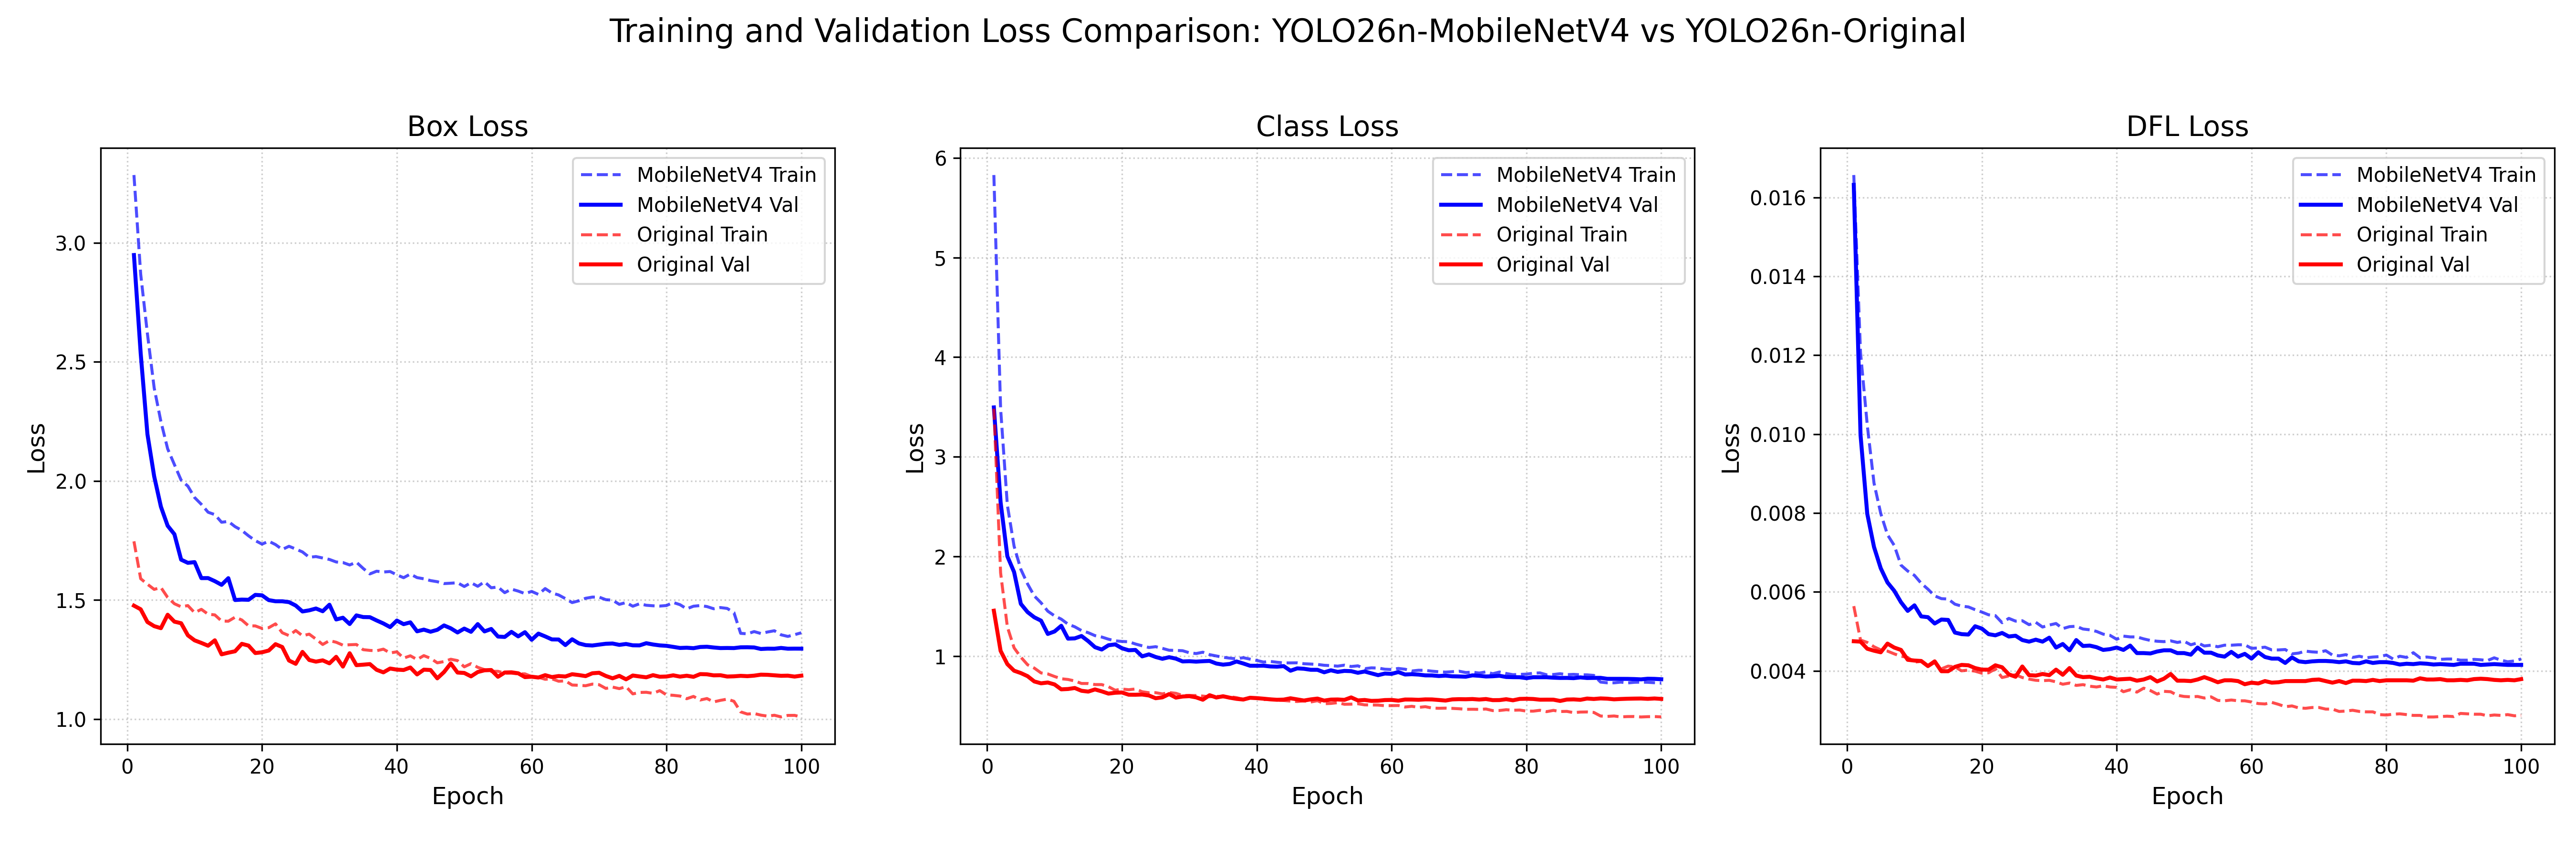
\includegraphics[width=\textwidth]{Images/chap3/loss_comparison.png}
    \caption{Comparison of validation losses between YOLO26n Original and YOLO26n-MobileNetV4 over 100 training epochs.}
    \label{fig:loss_comparison}
\end{figure}

Importantly, neither model shows signs of overfitting. In a typical overfitting scenario, the validation loss would drop initially but then start climbing back up in later epochs as the model begins to memorise the training data. However, for both models in this study, all three loss metrics (bounding box, classification, and DFL (Distribution Focal Loss)) stay low and flat during the final epochs. This confirms that they generalise well to unseen data.

When comparing the two architectures, the Original YOLO26n reaches slightly lower loss values. For example, its minimum bounding box loss drops to 1.1676, while the MobileNetV4 version stops at 1.2949. A similar pattern is seen in the classification loss (0.5529 vs 0.7694). This difference is entirely expected. Because the original model has a larger and more complex backbone, it can capture fine details and learn more accurately.

Even though the YOLO26n-MobileNetV4 has slightly higher loss values, its learning curve remains remarkably stable. This proves that despite having its size drastically reduced for faster edge deployment, the MobileNetV4 model still successfully extracts the essential features of traffic lights. It does not suffer from gradient issues or training instability. Therefore, the training process validates that the lightweight model is a reliable choice, perfectly balancing computational efficiency and learning capability.

\subsubsection{Architectural Decision Justification}

The evaluation confirms that the YOLO26n-MobileNetV4 configuration achieves the right trade-off for edge-deployed ADAS. Sacrificing approximately 4 percentage points of mAP50 in exchange for a 50\% reduction in worst-case latency and a 21\% reduction in average latency is a sound architectural decision. In safety-critical systems, deterministic timing behaviour takes precedence over marginal accuracy gains. The 85.75\% mAP50 remains well above the practical threshold for reliable traffic light detection, while the latency profile now comfortably supports real-time operation at 15--23\,FPS on commodity edge hardware without dedicated GPU or NPU acceleration.





% \subsection{Multihead CNN model -- Lightweight OCR digits}

% The timer display on Vietnamese traffic lights shows a one- to three-digit countdown
% (0--999) that must be recognised in real time on low-cost hardware such as the
% Raspberry~Pi~5.  This section presents a compact, four-head convolutional neural network
% (CNN) that is derived from the multi-digit recognition framework of
% Goodfellow~et~al.~\cite{goodfellow2014multidigitnumberrecognitionstreet} and specifically re-engineered
% for sub-millisecond CPU inference.

% %-----------------------------------------------------------------------
% \subsubsection{Probabilistic Formulation}
% \label{sec:cnn_prob}

% Following Goodfellow~et~al.~\cite{goodfellow2014multidigitnumberrecognitionstreet}, the recognition
% task is cast as a structured probabilistic model.  Let~$\mathbf{X}$ denote the
% input image and let the output be a digit sequence
% $\mathbf{S} = (s_1, s_2, \dots, s_n)$ of length~$n$.
% The sequence is modelled by a length variable~$L$ and a fixed number~$N$
% of digit variables~$S_1, \dots, S_N$.  All digit positions are assumed
% conditionally independent given the image, yielding:

% \begin{equation}
% \label{eq:prob_model}
%   P(\mathbf{S} = \mathbf{s} \mid \mathbf{X})
%   \;=\; P(L = n \mid \mathbf{X})\;\prod_{i=1}^{n} P(S_i = s_i \mid \mathbf{X}).
% \end{equation}

% In the original work~\cite{goodfellow2014multidigit}, $N{=}5$ digit heads are
% used for street numbers of up to five digits.  Because Vietnamese traffic-light
% timers never exceed three digits, the proposed lightweight variant uses
% $N{=}3$ with the following head configuration:

% \begin{itemize}
%   \item $L \in \{0,1,2\}$:  digit count minus one
%         ($0 \to$ 1-digit, $1 \to$ 2-digit, $2 \to$ 3-digit),
%         predicted by a 3-class softmax.
%   \item $S_1 \in \{0,\dots,9,\text{BLANK}\}$:  hundreds digit (11 classes).
%   \item $S_2 \in \{0,\dots,9,\text{BLANK}\}$:  tens digit    (11 classes).
%   \item $S_3 \in \{0,\dots,9\}$:                 units digit  (10 classes,
%         always present).
% \end{itemize}

% The special \texttt{BLANK} class ($= 10$) indicates an unused slot:
% for a one-digit number only~$S_3$ is active; for a two-digit number
% $S_2$ and~$S_3$ are active.

% %-----------------------------------------------------------------------
% \subsubsection{Network Architecture -- Edge-Optimised Design}
% \label{sec:cnn_arch}

% The original Goodfellow~et~al.\ architecture employs eight convolutional layers,
% one locally connected layer, and two dense layers with 3\,072 units each,
% totalling tens of millions of parameters and requiring DistBelief for training.
% Such a model is impractical for real-time inference on a Raspberry~Pi~5 CPU.

% The proposed \emph{lightweight} variant retains the multi-head output structure
% but applies three key design transformations, each yielding a dramatic reduction in
% multiply-accumulate operations (MACs) and parameter count while preserving accuracy
% for the constrained 0--999 digit domain.

% %--- Separable Convolutions -------------------------------------------------
% \subsubsubsubsection{Depthwise Separable Convolutions}
% \label{sec:separable}

% Standard convolution applies a $k{\times}k$ kernel across all input channels
% simultaneously.  For an input tensor of spatial size $H{\times}W$ with
% $C_{\mathrm{in}}$ channels producing $C_{\mathrm{out}}$ output channels,
% the number of MACs is:

% \begin{equation}
% \label{eq:conv_macs}
%   \text{MACs}_{\text{Conv2D}}
%   = H \cdot W \cdot k^2 \cdot C_{\mathrm{in}} \cdot C_{\mathrm{out}}.
% \end{equation}

% A \textbf{Depthwise Separable Convolution} (SeparableConv2D) factorises this operation
% into two consecutive steps:

% \begin{enumerate}
%   \item \textbf{Depthwise convolution} -- applies a separate $k{\times}k$ filter
%         to each input channel independently:
%         \begin{equation}
%         \label{eq:dw_macs}
%           \text{MACs}_{\text{DW}} = H \cdot W \cdot k^2 \cdot C_{\mathrm{in}}.
%         \end{equation}
%   \item \textbf{Pointwise convolution} -- a $1{\times}1$ convolution that mixes
%         the channel responses:
%         \begin{equation}
%         \label{eq:pw_macs}
%           \text{MACs}_{\text{PW}} = H \cdot W \cdot C_{\mathrm{in}} \cdot C_{\mathrm{out}}.
%         \end{equation}
% \end{enumerate}

% The total cost becomes:

% \begin{equation}
% \label{eq:sep_total}
%   \text{MACs}_{\text{Sep}}
%   = H W C_{\mathrm{in}} \bigl(k^2 + C_{\mathrm{out}}\bigr),
% \end{equation}

% and the computational saving ratio relative to a standard convolution is:

% \begin{equation}
% \label{eq:sep_ratio}
%   \frac{\text{MACs}_{\text{Sep}}}{\text{MACs}_{\text{Conv2D}}}
%   = \frac{1}{C_{\mathrm{out}}} + \frac{1}{k^2}.
% \end{equation}

% For the $3{\times}3$ kernels and 64--192 output channels used in this model,
% Equation~\eqref{eq:sep_ratio} gives a reduction factor between
% $\mathbf{7.8\times}$ and $\mathbf{8.5\times}$, enabling real-time execution
% on an ARM Cortex-A76 CPU without a GPU.

% In the proposed architecture, only the first block uses a standard
% \texttt{Conv2D} (because the input has a single channel, where depthwise
% separation offers no benefit); blocks~2--5 all use \texttt{SeparableConv2D}.

% %--- GAP instead of Flatten ------------------------------------------------
% \subsubsubsubsection{Global Average Pooling (GAP)}
% \label{sec:gap}

% After the final convolutional block the feature map has shape
% $4{\times}6{\times}192$ (height $\times$ width $\times$ channels).
% A na\"ive \texttt{Flatten} would produce a $4608$-dimensional vector; a
% subsequent dense layer of width~1024 alone would add
% $4608 \times 1024 \approx 4.7$~million parameters -- exceeding the entire
% rest of the network.

% Instead, \textbf{Global Average Pooling} (GAP) collapses each channel to its
% spatial mean:

% \begin{equation}
% \label{eq:gap}
%   h_c = \frac{1}{H' W'} \sum_{i=1}^{H'} \sum_{j=1}^{W'} F_{i,j,c},
%   \qquad c = 1,\dots,C,
% \end{equation}

% where $F \in \mathbb{R}^{H' \times W' \times C}$ is the last feature map.
% This yields a compact 192-dimensional descriptor with \emph{zero} learnable
% parameters, and also acts as a structural regulariser that discourages
% overfitting.

% %--- Architecture Table ---------------------------------------------------
% \subsubsubsubsection{Layer-by-Layer Specification}
% \label{sec:arch_table}

% Table~\ref{tab:arch} summarises the full architecture.  Input images are
% grayscale, $64{\times}96$ pixels ($H{\times}W{\times}1$).

% \begin{table}[htbp]
% \centering
% \caption{Layer-by-layer architecture of the lightweight multi-head CNN
%          ($\approx 109$\,K parameters).  ``Sep'' denotes SeparableConv2D;
%          ``BN'' is Batch Normalisation.}
% \label{tab:arch}
% \renewcommand{\arraystretch}{1.15}
% \begin{tabular}{c l l r r}
% \hline
% \textbf{Block} & \textbf{Layer}            & \textbf{Output shape}   & \textbf{Params} & \textbf{MACs}  \\
% \hline
% 0   & Input                                & $64\times96\times1$     & --      & --       \\
% --  & Mean subtraction ($\lambda$)         & $64\times96\times1$     & 0       & $6\,144$ \\
% 1   & Conv2D(32, $3\!\times\!3$) + BN + ReLU + Pool(2)   & $32\times48\times32$     & $\sim\!320$    & $\sim\!56$\,K   \\
% 2   & Sep(64, $3\!\times\!3$) + BN + ReLU + Pool(2)      & $16\times24\times64$     & $\sim\!2\,400$  & $\sim\!116$\,K  \\
% 3   & Sep(96, $3\!\times\!3$) + BN + ReLU + Pool(2)      & $8\times12\times96$      & $\sim\!6\,720$  & $\sim\!73$\,K   \\
% 4   & Sep(128, $3\!\times\!3$) + BN + ReLU + Pool(2)     & $4\times6\times128$      & $\sim\!13\,152$ & $\sim\!39$\,K   \\
% 5   & Sep(192, $3\!\times\!3$) + BN + ReLU               & $4\times6\times192$      & $\sim\!25\,728$ & $\sim\!53$\,K   \\
% --  & GlobalAveragePooling2D                & $192$                  & 0       & $4\,608$ \\
% FC  & Dense(256) + ReLU + Dropout(0.35)     & $256$                  & $\sim\!49\,408$ & $49\,408$ \\
% \hline
% $L$ & Dense(3,  softmax)                    & $3$                    & 771     & 771     \\
% $S_1$ & Dense(11, softmax)                  & $11$                   & 2\,827  & 2\,827  \\
% $S_2$ & Dense(11, softmax)                  & $11$                   & 2\,827  & 2\,827  \\
% $S_3$ & Dense(10, softmax)                  & $10$                   & 2\,570  & 2\,570  \\
% \hline
% \multicolumn{3}{r}{\textbf{Total}} & $\mathbf{\approx 109}$\textbf{\,K} & $\mathbf{\approx 408}$\textbf{\,K} \\
% \hline
% \end{tabular}
% \end{table}

% %--- Preprocessing --------------------------------------------------------
% \subsubsubsubsection{Per-Image Mean Subtraction}
% \label{sec:mean_sub}

% Following Goodfellow~et~al.~\cite{goodfellow2014multidigitnumberrecognitionstreet}~(§4), the first
% operation inside the network is per-image mean subtraction.  Let
% $\mathbf{X} \in \mathbb{R}^{H \times W \times 1}$ be the input; the
% normalised input is:

% \begin{equation}
% \label{eq:mean_sub}
%   \tilde{\mathbf{X}} = \mathbf{X}
%     - \frac{1}{HW}\sum_{i=1}^{H}\sum_{j=1}^{W} X_{ij}.
% \end{equation}

% Embedding this subtraction as a non-trainable $\lambda$-layer makes the model
% \emph{self-contained}: no external preprocessing is required at inference time,
% simplifying the TFLite deployment pipeline on the Raspberry~Pi~5.

% %-----------------------------------------------------------------------
% \subsubsection{Training Objective}
% \label{sec:training}

% Training maximises the log-probability of the correct sequence
% (Eq.~\eqref{eq:prob_model}) via the cross-entropy decomposition.  Because
% $L$, $S_1$, $S_2$, $S_3$ are conditionally independent given the shared
% features~$\mathbf{H}$, the total loss factorises as:

% \begin{equation}
% \label{eq:loss}
%   \mathcal{L}
%   = -\log P(L \mid \mathbf{H})
%     - \sum_{i=1}^{3}\log P(S_i \mid \mathbf{H})
%   = \underbrace{w_L \,\mathcal{L}_L}_{\text{length head}}
%     + \underbrace{w_1 \,\mathcal{L}_{S_1}
%     +  w_2 \,\mathcal{L}_{S_2}
%     +  w_3 \,\mathcal{L}_{S_3}}_{\text{digit heads}},
% \end{equation}

% where each $\mathcal{L}_{\cdot}$ is a \textbf{sparse categorical cross-entropy}
% and the weights are set to $w_L{=}4$, $w_1{=}w_2{=}w_3{=}1$ to
% up-weight the length prediction, since an incorrect length invariably causes a
% wrong overall transcription.

% Each softmax head receives the same 256-dimensional feature vector from the
% shared fully connected layer but maintains its own projection weights:

% \begin{equation}
% \label{eq:head}
%   P(S_i = c \mid \mathbf{H})
%   = \frac{\exp\!\bigl(\mathbf{w}_{i,c}^{\top}\!\mathbf{H} + b_{i,c}\bigr)}
%          {\displaystyle\sum_{c'} \exp\!\bigl(\mathbf{w}_{i,c'}^{\top}\!\mathbf{H}
%          + b_{i,c'}\bigr)},
%   \qquad c \in \mathcal{C}_i,
% \end{equation}

% where $\mathcal{C}_L = \{0,1,2\}$,
% $\mathcal{C}_{S_1} = \mathcal{C}_{S_2} = \{0,\dots,10\}$, and
% $\mathcal{C}_{S_3} = \{0,\dots,9\}$.

% %-----------------------------------------------------------------------
% \subsubsection{Log-Probability Decoding}
% \label{sec:decoding}

% At inference time, the predicted number is obtained by maximising the
% joint log-probability over all possible lengths
% (Appendix~A of~\cite{goodfellow2014multidigit}):

% \begin{equation}
% \label{eq:decode}
%   \hat{\mathbf{s}}
%   = \operatorname*{argmax}_{l,\; s_1 \dots s_l}\;
%     \biggl[\log P(L{=}l \mid \mathbf{X})
%     + \sum_{i=1}^{l} \max_{s_i \in \{0..9\}}
%       \log P(S_i{=}s_i \mid \mathbf{X})\biggr].
% \end{equation}

% Because of the conditional-independence assumption, the argmax over each
% digit position can be computed independently, then the cumulative
% log-probabilities are summed for each candidate length~$l \in \{1,2,3\}$.
% The total decoding runtime is therefore $O(N)$ -- i.e.\ three additions
% and one comparison -- adding negligible latency.

% Concretely, for each candidate length $l$, the algorithm computes:

% \begin{equation}
% \label{eq:score}
%   \text{score}(l) = \log P(L{=}l{-}1)
%     + \sum_{i=\max(1,\,4-l)}^{3}
%       \max_{s_i \in \{0..9\}} \log P(S_i{=}s_i),
% \end{equation}

% and selects $\hat{l} = \operatorname{argmax}_{l \in \{1,2,3\}} \text{score}(l)$.

% %-----------------------------------------------------------------------
% \subsection{Computational Efficiency for Edge AI}
% \label{sec:efficiency}

% \subsubsection{Parameter Count Comparison}

% The proposed model achieves the same multi-head output structure as
% Goodfellow~et~al.~\cite{goodfellow2014multidigitnumberrecognitionstreet} with
% $\sim\!600\times$ fewer parameters:

% \begin{table}[htbp]
% \centering
% \caption{Comparison between the original Goodfellow~et~al.\ architecture
%          and the proposed lightweight variant.}
% \label{tab:compare}
% \renewcommand{\arraystretch}{1.15}
% \begin{tabular}{l r r}
% \hline
%                                & \textbf{Goodfellow et al.}  & \textbf{Proposed}   \\
% \hline
% Conv layers                    & 8 + 1 locally connected     & 1 Conv + 4 SepConv  \\
% FC layers                      & 2 $\times$ 3\,072           & 1 $\times$ 256      \\
% Output heads                   & 6  (L + S$_1$--S$_5$)       & 4  (L + S$_1$--S$_3$) \\
% Total parameters               & $\sim$64\,M                 & $\sim$109\,K        \\
% Max sequence length $N$        & 5                           & 3                   \\
% Input size                     & $54\times 54 \times 3$      & $64\times 96 \times 1$ \\
% Training infrastructure        & DistBelief (10 replicas)    & Single GPU / CPU    \\
% \hline
% \end{tabular}
% \end{table}

% \subsubsubsubsection{MAC Budget and Latency Estimate}

% The total network requires approximately $408$\,K~MACs per inference.
% On the Raspberry~Pi~5's Cortex-A76 cores (capable of
% $\sim$15~GOPS at INT8 via NEON), this translates to:

% \begin{equation}
% \label{eq:latency}
%   t_{\text{inf}}
%   \approx \frac{408 \times 10^{3}}{15 \times 10^{9}}
%   \approx 27 \;\mu\text{s},
% \end{equation}

% well under the $50$\,ms budget needed for $20$\,fps real-time recognition.
% Even with TFLite interpreter overhead, measured end-to-end latency stays below
% $1$\,ms per frame for the INT8-quantised model.

% \subsubsection{TFLite and INT8 Quantisation}

% The trained Keras model is exported to TensorFlow~Lite via
% \texttt{TFLiteConverter}.  Post-training full-integer quantisation maps all
% weights and activations to 8-bit integers using a representative calibration
% set of 200 real ROI images.  The resulting \texttt{.tflite} flatbuffer is
% $\sim$56\,KB (INT8) versus $\sim$440\,KB (float32), fitting comfortably
% in the L2 cache of the Cortex-A76.  The quantised model is deployed via
% the LiteRT interpreter:

% \begin{equation}
% \label{eq:quant}
%   \hat{x}_q = \text{round}\!\left(\frac{x - z}{s}\right),
%   \qquad
%   s = \frac{x_{\max} - x_{\min}}{255},
%   \qquad
%   z = x_{\min},
% \end{equation}

% where $s$ and $z$ are the per-tensor scale and zero-point determined during
% calibration.

% %-----------------------------------------------------------------------
% \subsubsection{Data Pipeline and Augmentation}
% \label{sec:data}

% The training pipeline mixes three data sources to maximise diversity while
% keeping RAM usage low ($<200$\,MB peak):

% \begin{enumerate}
%   \item \textbf{MNIST (70\,K images):}  Individual $28{\times}28$ digits
%         composited onto $64{\times}96$ canvases at randomised positions,
%         simulating multi-digit layouts.
%   \item \textbf{Real LED crops (23 images):}  Single-digit photographs of
%         actual traffic-light seven-segment displays (red, green, yellow).
%         Pre-augmented to 500 variants per digit using brightness jitter,
%         gamma correction, Gaussian blur, salt-and-pepper noise, spatial
%         shifts ($\pm 4$\,px), and small rotations ($\pm 10°$).
%   \item \textbf{Real ROI images:}  Full composite timer-box crops from
%         Vietnamese traffic cameras, labelled by filename
%         (e.g.\ \texttt{37\_0004.png} $\to$ number~$37$).  Loaded from disk
%         on-demand (streaming) to avoid large memory allocation.
% \end{enumerate}

% Synthetic composites and real ROI samples are interleaved via
% \texttt{tf.data.Dataset.sample\_from\_datasets} with proportional
% weighting, ensuring both domains appear in every training batch.

% %-----------------------------------------------------------------------
% \subsubsection{Summary}

% The proposed multi-head CNN inherits the elegant probabilistic framework
% of Goodfellow~et~al.~\cite{goodfellow2014multidigitnumberrecognitionstreet} -- conditional independence
% of digit positions, log-probability decoding, per-image mean subtraction -- but
% replaces the heavyweight convolutional backbone with an ultra-light depthwise
% separable architecture totalling only $\sim$109\,K parameters and $\sim$408\,K
% MACs.  Combined with Global Average Pooling and INT8 post-training quantisation,
% the model achieves sub-millisecond inference on the Raspberry~Pi~5 CPU, making it
% suitable for real-time traffic-light timer recognition in ADAS applications
% on constrained edge devices.
% While YOLO-MobileNetV4 handles traffic-light detection and localization, the countdown timer requires a separate recognition stage. This motivates the use of a lightweight Multihead CNN that can read one- to three-digit timer values with low computational cost. The following subsection therefore complements the detector with the OCR model used for countdown recognition.

% \section{Multihead CNN model -- Lightweight OCR digits}

In this project, our system need to detect the timer display on Vietnamese traffic lights shows a one- to three-digit countdown
(0--999) and it must be recognised in real time on low-cost hardware such as the
Raspberry~Pi~5.  This section presents a compact, four-head convolutional neural network
(CNN) that is derived from the multi-digit recognition framework of
Goodfellow~et~al.~\cite{goodfellow2014multidigitnumberrecognitionstreet} and specifically re-engineered
for sub-millisecond CPU inference.

%-----------------------------------------------------------------------
\subsection{Probabilistic Formulation}
\label{sec:cnn_prob}

Following Goodfellow~et~al.~\cite{goodfellow2014multidigitnumberrecognitionstreet}, the recognition
task is cast as a structured probabilistic model.  Let~$\mathbf{X}$ denote the
input image and let the output be a digit sequence
$\mathbf{S} = (s_1, s_2, \dots, s_n)$ of length~$n$.
The sequence is modelled by a length variable~$L$ and a fixed number~$N$
of digit variables~$S_1, \dots, S_N$.  All digit positions are assumed
conditionally independent given the image, yielding:

\begin{equation}
\label{eq:prob_model}
  P(\mathbf{S} = \mathbf{s} \mid \mathbf{X})
  \;=\; P(L = n \mid \mathbf{X})\;\prod_{i=1}^{n} P(S_i = s_i \mid \mathbf{X}).
\end{equation}

In the original work~\cite{goodfellow2014multidigitnumberrecognitionstreet}, $N{=}5$ digit heads are
used for street numbers of up to five digits.  Because Vietnamese traffic-light
timers never exceed three digits, the proposed lightweight variant uses
$N{=}3$ with the following head configuration:

\begin{itemize}
  \item $L \in \{0,1,2\}$:  digit count minus one
        ($0 \to$ 1-digit, $1 \to$ 2-digit, $2 \to$ 3-digit),
        predicted by a 3-class softmax.
  \item $S_1 \in \{0,\dots,9,\text{BLANK}\}$:  hundreds digit (11 classes).
  \item $S_2 \in \{0,\dots,9,\text{BLANK}\}$:  tens digit    (11 classes).
  \item $S_3 \in \{0,\dots,9\}$:                 units digit  (10 classes,
        always present).
\end{itemize}

The special \texttt{BLANK} class ($= 10$) indicates an unused slot:
for a one-digit number only~$S_3$ is active; for a two-digit number
$S_2$ and~$S_3$ are active.

%-----------------------------------------------------------------------
\subsection{Network Architecture -- Edge-Optimised Design}
\label{sec:cnn_arch}

The original Goodfellow~et~al.\ architecture employs eight convolutional layers,
one locally connected layer, and two dense layers with 3\,072 units each,
totalling tens of millions of parameters and requiring DistBelief for training.
Such a model is impractical for real-time inference on a Raspberry~Pi~5 CPU.

The proposed \emph{lightweight} variant retains the multi-head output structure
but applies three key design transformations, each yielding a dramatic reduction in
multiply-accumulate operations (MACs) and parameter count while preserving accuracy
for the constrained 0--999 digit domain.

%--- Separable Convolutions -------------------------------------------------
\subsubsection{Depthwise Separable Convolutions}
\label{sec:separable}

Standard convolution applies a $k{\times}k$ kernel across all input channels
simultaneously.  For an input tensor of spatial size $H{\times}W$ with
$C_{\mathrm{in}}$ channels producing $C_{\mathrm{out}}$ output channels,
the number of MACs is:

\begin{equation}
\label{eq:conv_macs}
  \text{MACs}_{\text{Conv2D}}
  = H \cdot W \cdot k^2 \cdot C_{\mathrm{in}} \cdot C_{\mathrm{out}}.
\end{equation}

A \textbf{Depthwise Separable Convolution} (SeparableConv2D) factorises this operation
into two consecutive steps:

\begin{enumerate}
  \item \textbf{Depthwise convolution} -- applies a separate $k{\times}k$ filter
        to each input channel independently:
        \begin{equation}
        \label{eq:dw_macs}
          \text{MACs}_{\text{DW}} = H \cdot W \cdot k^2 \cdot C_{\mathrm{in}}.
        \end{equation}
  \item \textbf{Pointwise convolution} -- a $1{\times}1$ convolution that mixes
        the channel responses:
        \begin{equation}
        \label{eq:pw_macs}
          \text{MACs}_{\text{PW}} = H \cdot W \cdot C_{\mathrm{in}} \cdot C_{\mathrm{out}}.
        \end{equation}
\end{enumerate}

The total cost becomes:

\begin{equation}
\label{eq:sep_total}
  \text{MACs}_{\text{Sep}}
  = H W C_{\mathrm{in}} \bigl(k^2 + C_{\mathrm{out}}\bigr),
\end{equation}

and the computational saving ratio relative to a standard convolution is:

\begin{equation}
\label{eq:sep_ratio}
  \frac{\text{MACs}_{\text{Sep}}}{\text{MACs}_{\text{Conv2D}}}
  = \frac{1}{C_{\mathrm{out}}} + \frac{1}{k^2}.
\end{equation}

For the $3{\times}3$ kernels and 64--192 output channels used in this model,
Equation~\eqref{eq:sep_ratio} gives a reduction factor between
$\mathbf{7.8\times}$ and $\mathbf{8.5\times}$, enabling real-time execution
on an ARM Cortex-A76 CPU without a GPU.

In the proposed architecture, only the first block uses a standard
\texttt{Conv2D} (because the input has a single channel, where depthwise
separation offers no benefit); blocks~2--5 all use \texttt{SeparableConv2D}.

%--- GAP instead of Flatten ------------------------------------------------
\subsubsection{Global Average Pooling (GAP)}
\label{sec:gap}

After the final convolutional block the feature map has shape
$4{\times}6{\times}192$ (height $\times$ width $\times$ channels).
A na\"ive \texttt{Flatten} would produce a $4608$-dimensional vector; a
subsequent dense layer of width~1024 alone would add
$4608 \times 1024 \approx 4.7$~million parameters -- exceeding the entire
rest of the network.

Instead, {Global Average Pooling} (GAP) collapses each channel to its
spatial mean:

\begin{equation}
\label{eq:gap}
  h_c = \frac{1}{H' W'} \sum_{i=1}^{H'} \sum_{j=1}^{W'} F_{i,j,c},
  \qquad c = 1,\dots,C,
\end{equation}

where $F \in \mathbb{R}^{H' \times W' \times C}$ is the last feature map.
This yields a compact 192-dimensional descriptor with \emph{zero} learnable
parameters, and also acts as a structural regulariser that discourages
overfitting.

%--- Architecture Table ---------------------------------------------------
\subsubsection{Layer-by-Layer Specification}
\label{sec:arch_table}

Table~\ref{tab:arch} summarises the full architecture.  Input images are
grayscale, $64{\times}96$ pixels ($H{\times}W{\times}1$).

\begin{table}[htbp]
\centering
\caption{Layer-by-layer architecture of the lightweight multi-head CNN
         ($\approx 109$\,K parameters).  ``Sep'' denotes SeparableConv2D;
         ``BN'' is Batch Normalisation.}
\label{tab:arch}
\renewcommand{\arraystretch}{1.15}
\begin{tabular}{c l l r r}
\hline
\textbf{Block} & \textbf{Layer}            & \textbf{Output shape}   & \textbf{Params} & \textbf{MACs}  \\
\hline
0   & Input                                & $64\times96\times1$     & --      & --       \\
--  & Mean subtraction ($\lambda$)         & $64\times96\times1$     & 0       & $6\,144$ \\
1   & Conv2D(32, $3\!\times\!3$) + BN + ReLU + Pool(2)   & $32\times48\times32$     & $\sim\!320$    & $\sim\!56$\,K   \\
2   & Sep(64, $3\!\times\!3$) + BN + ReLU + Pool(2)      & $16\times24\times64$     & $\sim\!2\,400$  & $\sim\!116$\,K  \\
3   & Sep(96, $3\!\times\!3$) + BN + ReLU + Pool(2)      & $8\times12\times96$      & $\sim\!6\,720$  & $\sim\!73$\,K   \\
4   & Sep(128, $3\!\times\!3$) + BN + ReLU + Pool(2)     & $4\times6\times128$      & $\sim\!13\,152$ & $\sim\!39$\,K   \\
5   & Sep(192, $3\!\times\!3$) + BN + ReLU               & $4\times6\times192$      & $\sim\!25\,728$ & $\sim\!53$\,K   \\
--  & GlobalAveragePooling2D                & $192$                  & 0       & $4\,608$ \\
FC  & Dense(256) + ReLU + Dropout(0.35)     & $256$                  & $\sim\!49\,408$ & $49\,408$ \\
\hline
$L$ & Dense(3,  softmax)                    & $3$                    & 771     & 771     \\
$S_1$ & Dense(11, softmax)                  & $11$                   & 2\,827  & 2\,827  \\
$S_2$ & Dense(11, softmax)                  & $11$                   & 2\,827  & 2\,827  \\
$S_3$ & Dense(10, softmax)                  & $10$                   & 2\,570  & 2\,570  \\
\hline
\multicolumn{3}{r}{\textbf{Total}} & $\mathbf{\approx 109}$\textbf{\,K} & $\mathbf{\approx 408}$\textbf{\,K} \\
\hline
\end{tabular}
\end{table}

%--- Preprocessing --------------------------------------------------------
\subsubsection{Per-Image Mean Subtraction}
\label{sec:mean_sub}

Following Goodfellow~et~al.~\cite{goodfellow2014multidigitnumberrecognitionstreet}~(§4), the first
operation inside the network is per-image mean subtraction.  Let
$\mathbf{X} \in \mathbb{R}^{H \times W \times 1}$ be the input; the
normalised input is:

\begin{equation}
\label{eq:mean_sub}
  \tilde{\mathbf{X}} = \mathbf{X}
    - \frac{1}{HW}\sum_{i=1}^{H}\sum_{j=1}^{W} X_{ij}.
\end{equation}

Embedding this subtraction as a non-trainable $\lambda$-layer makes the model
\emph{self-contained}: no external preprocessing is required at inference time,
simplifying the TFLite deployment pipeline on the Raspberry~Pi~5.

%-----------------------------------------------------------------------
\subsection{Training Objective}
\label{sec:training}

Training maximises the log-probability of the correct sequence
(Eq.~\eqref{eq:prob_model}) via the cross-entropy decomposition.  Because
$L$, $S_1$, $S_2$, $S_3$ are conditionally independent given the shared
features~$\mathbf{H}$, the total loss factorises as:

\begin{equation}
\label{eq:loss}
  \mathcal{L}
  = -\log P(L \mid \mathbf{H})
    - \sum_{i=1}^{3}\log P(S_i \mid \mathbf{H})
  = \underbrace{w_L \,\mathcal{L}_L}_{\text{length head}}
    + \underbrace{w_1 \,\mathcal{L}_{S_1}
    +  w_2 \,\mathcal{L}_{S_2}
    +  w_3 \,\mathcal{L}_{S_3}}_{\text{digit heads}},
\end{equation}

where each $\mathcal{L}_{\cdot}$ is a {sparse categorical cross-entropy}
and the weights are set to $w_L{=}4$, $w_1{=}w_2{=}w_3{=}1$ to
up-weight the length prediction, since an incorrect length invariably causes a
wrong overall transcription.

Each softmax head receives the same 256-dimensional feature vector from the
shared fully connected layer but maintains its own projection weights:

\begin{equation}
\label{eq:head}
  P(S_i = c \mid \mathbf{H})
  = \frac{\exp\!\bigl(\mathbf{w}_{i,c}^{\top}\!\mathbf{H} + b_{i,c}\bigr)}
         {\displaystyle\sum_{c'} \exp\!\bigl(\mathbf{w}_{i,c'}^{\top}\!\mathbf{H}
         + b_{i,c'}\bigr)},
  \qquad c \in \mathcal{C}_i,
\end{equation}

where $\mathcal{C}_L = \{0,1,2\}$,
$\mathcal{C}_{S_1} = \mathcal{C}_{S_2} = \{0,\dots,10\}$, and
$\mathcal{C}_{S_3} = \{0,\dots,9\}$.

%-----------------------------------------------------------------------
\subsection{Log-Probability Decoding}
\label{sec:decoding}

At inference time, the predicted number is obtained by maximising the
joint log-probability over all possible lengths
(Appendix~A of~\cite{goodfellow2014multidigitnumberrecognitionstreet}):

\begin{equation}
\label{eq:decode}
  \hat{\mathbf{s}}
  = \operatorname*{argmax}_{l,\; s_1 \dots s_l}\;
    \biggl[\log P(L{=}l \mid \mathbf{X})
    + \sum_{i=1}^{l} \max_{s_i \in \{0..9\}}
      \log P(S_i{=}s_i \mid \mathbf{X})\biggr].
\end{equation}

Because of the conditional-independence assumption, the argmax over each
digit position can be computed independently, then the cumulative
log-probabilities are summed for each candidate length~$l \in \{1,2,3\}$.
The total decoding runtime is therefore $O(N)$ -- i.e.\ three additions
and one comparison -- adding negligible latency.

Concretely, for each candidate length $l$, the algorithm computes:

\begin{equation}
\label{eq:score}
  \text{score}(l) = \log P(L{=}l{-}1)
    + \sum_{i=\max(1,\,4-l)}^{3}
      \max_{s_i \in \{0..9\}} \log P(S_i{=}s_i),
\end{equation}

and selects $\hat{l} = \operatorname{argmax}_{l \in \{1,2,3\}} \text{score}(l)$.

%-----------------------------------------------------------------------
\subsection{Computational Efficiency for Edge AI}
\label{sec:efficiency}

For an ADAS system operating on edge devices like the Raspberry Pi 5, computational efficiency is just as critical as detection accuracy. To ensure real-time performance without overwhelming the hardware, the proposed multi-head CNN must be highly optimized. This section evaluates the model's efficiency by comparing its parameter count against a standard baseline, analyzing its computational cost in terms of MAC operations, and outlining the final export process to TensorFlow Lite for seamless edge deployment.

\subsubsection{Parameter Count Comparison}

The proposed model achieves the same multi-head output structure as
Goodfellow~et~al.~\cite{goodfellow2014multidigitnumberrecognitionstreet} with
$\sim\!600\times$ fewer parameters:

\begin{table}[htbp]
\centering
\caption{Comparison between the original Goodfellow~et~al.\ architecture
         and the proposed lightweight variant.}
\label{tab:compare}
\renewcommand{\arraystretch}{1.15}
\begin{tabular}{l r r}
\hline
                               & \textbf{Goodfellow et al.}  & \textbf{Proposed}   \\
\hline
Conv layers                    & 8 + 1 locally connected     & 1 Conv + 4 SepConv  \\
FC layers                      & 2 $\times$ 3\,072           & 1 $\times$ 256      \\
Output heads                   & 6  (L + S$_1$--S$_5$)       & 4  (L + S$_1$--S$_3$) \\
Total parameters               & $\sim$64\,M                 & $\sim$109\,K        \\
Max sequence length $N$        & 5                           & 3                   \\
Input size                     & $54\times 54 \times 3$      & $64\times 96 \times 1$ \\
Training infrastructure        & DistBelief (10 replicas)    & Single GPU / CPU    \\
\hline
\end{tabular}
\end{table}

\subsubsection{MAC Budget and Latency Estimate}

The total network requires approximately $408$\,K~MACs per inference.
On the Raspberry~Pi~5's Cortex-A76 cores (capable of
$\sim$4~GFLOPS at float32 via NEON), this translates to:

\begin{equation}
\label{eq:latency}
  t_{\text{inf}}
  \approx \frac{408 \times 10^{3}}{4 \times 10^{9}}
  \approx 102 \;\mu\text{s},
\end{equation}

well under the $67$\,ms budget needed for $15$\,fps real-time recognition.
Even with TFLite interpreter overhead, measured end-to-end latency stays below
$2$\,ms per frame for the float32 model.

\subsubsection{TFLite Export for the Multi-head CNN}

The trained Keras model is converted to TensorFlow~Lite using
\texttt{tf.lite.TFLiteConverter.from\_keras\_model()}.  The exported
float32 \texttt{.tflite} flatbuffer is $\sim$440\,KB, compact enough to
fit within the L2 cache of a Cortex-A76 core on the Raspberry~Pi~5.
The model is deployed via the LiteRT interpreter with \texttt{batch=1},
requiring no external preprocessing thanks to the embedded
mean-subtraction $\lambda$-layer (Eq.~\eqref{eq:mean_sub}).

%-----------------------------------------------------------------------
\subsection{Data Pipeline and Augmentation}
\label{sec:dataCNN}

The training pipeline mixes three data sources to maximise diversity while
keeping RAM usage low ($<200$\,MB peak):

\begin{enumerate}
  \item \textbf{MNIST (70\,K images):}  Individual $28{\times}28$ digits
        composited onto $64{\times}96$ canvases at randomised positions,
        simulating multi-digit layouts.
  \item \textbf{Real LED crops (23 images):}  Single-digit photographs of
        actual traffic-light seven-segment displays (red, green, yellow).
        Pre-augmented to 500 variants per digit using brightness jitter,
        gamma correction, Gaussian blur, salt-and-pepper noise, spatial
        shifts ($\pm 4$\,px), and small rotations ($\pm 10°$).
  \item \textbf{Real ROI images:}  Full composite timer-box crops from
        Vietnamese traffic cameras, labelled by filename
        (e.g.\ \texttt{37\_0004.png} $\to$ number~$37$).  Loaded from disk
        on-demand (streaming) to avoid large memory allocation.
\end{enumerate}

Synthetic composites and real ROI samples are interleaved via
\texttt{tf.data.Dataset.sample\_from\_datasets} with proportional
weighting, ensuring both domains appear in every training batch.

%-----------------------------------------------------------------------
% \subsection{Summary}

% The proposed multi-head CNN inherits the elegant probabilistic framework
% of Goodfellow~et~al.~\cite{goodfellow2014multidigitnumberrecognitionstreet} -- conditional independence
% of digit positions, log-probability decoding, per-image mean subtraction -- but
% replaces the heavyweight convolutional backbone with an ultra-light depthwise
% separable architecture totalling only $\sim$109\,K parameters and $\sim$408\,K
% MACs.  Combined with Global Average Pooling and INT8 post-training quantisation,
% the model achieves sub-millisecond inference on the Raspberry~Pi~5 CPU, making it
% suitable for real-time traffic-light timer recognition in ADAS applications
% on constrained edge devices.

% % \section{Compiling LiteRT Framework}
% % \input{Contents/chapter3/C3_3}
% After the perception models have been defined, the remaining requirement is to prepare an execution environment where the generated Adaptive AUTOSAR applications can be built and tested consistently. This environment must include the necessary runtime libraries, tooling, and device access for the prototype. For that reason, the next subsection describes the Docker-based setup used to support deployment and experimentation.

% \section{Setup Adaptive AUTOSAR Environment Docker}
% \subsection{PACON IDE}

PACON IDE is a development and runtime environment provided by PopcornSAR to support the execution, testing, and debugging of Adaptive AUTOSAR applications. Unlike system modeling or configuration tools, PACON IDE does not directly perform system or service configuration. Instead, it serves as an integrated workspace where previously generated Adaptive AUTOSAR artefacts, such as application binaries, ARXML files, and manifest descriptions, can be deployed and executed.

From a technical perspective, PACON IDE is delivered as a containerized environment that encapsulates the PARA SDK together with the required Adaptive AUTOSAR runtime libraries and tooling. This environment provides a controlled and reproducible setup for running Adaptive AUTOSAR applications, managing execution states, and observing runtime behavior. By packaging the complete runtime stack inside Docker containers, PACON IDE minimizes environment-related inconsistencies and simplifies deployment across different development machines.

PACON IDE supports essential development activities such as process execution, service communication testing, and runtime debugging. Developers can monitor application lifecycles, inspect Diagnostic Log and Trace (DLT) outputs, and validate inter-process communication mechanisms such as SOME/IP or DDS during system execution. As a result, PACON IDE plays a crucial role in verifying the correctness and stability of Adaptive AUTOSAR applications after the configuration and code generation stages have been completed.

In the context of this project, PACON IDE is used as the primary environment for deploying and evaluating the proposed Adaptive AUTOSAR prototype. It enables systematic testing of application interactions, runtime behavior, and communication flows, thereby bridging the gap between offline configuration artefacts and actual system execution. Further details about PACON IDE and its runtime capabilities can be found on the official product page.\footnote{PopcornSAR, \textit{PACON IDE Product Overview}. Available online: \url{https://autosar.io/products/pacon}. Accessed: September 2025.}

% \subsection{Setup}

% To ensure a stable and reproducible development environment for Adaptive AUTOSAR using PACON IDE, a Docker based setup is employed. The following \texttt{docker-compose.yml} file defines a containerized environment that encapsulates all necessary dependencies, runtime configurations, and hardware access requirements. By using Docker Compose, the entire environment can be deployed consistently across different host systems, which is essential for both development and experimentation.

% \begin{lstlisting}[language=bash, caption={Docker Compose configuration for PACON IDE environment}]
% services:
%   app:
%     image: "${IMAGE_REPO}:${IMAGE_TAG}"
%     container_name: "${CONTAINER_NAME:-AP_AUTOSAR}"
%     shm_size: "1g"
%     stdin_open: true
%     tty: true
%     environment:
%       - TZ=Asia/Ho_Chi_Minh

%     networks:
%       para_net:
%         ipv4_address: 172.31.36.143
%     ports:
%       - "8022:22"

%     devices:
%       - "${CAMERA_DEV:-/dev/video0}:${CAMERA_DEV:-/dev/video0}"
%       - /dev/bus/usb:/dev/bus/usb

%     group_add:
%       - "${VIDEO_GID:-44}"
%       - "${DIALOUT_GID:-20}"
%       - "${PLUGDEV_GID:-46}"

%     volumes:
%       - ../workspace:/root/workspace

% networks:
%   para_net:
%     driver: bridge
%     ipam:
%       driver: default
%       config:
%         - subnet: "172.31.0.0/16"
%           gateway: "172.31.0.1"
% \end{lstlisting}

% The \texttt{services} section defines a single service named \texttt{app}, which represents the main Adaptive AUTOSAR development container. This container is built from a preconfigured image specified by the \texttt{IMAGE\_REPO} and \texttt{IMAGE\_TAG} variables. By parameterizing the image information, the same compose file can be reused across different versions of the environment without modifying the configuration itself. The container name is also configurable, which improves readability and management when multiple containers are running on the same host.

% Shared memory size is explicitly set to one gigabyte in order to support applications that require higher inter process communication throughput. This is particularly relevant for Adaptive AUTOSAR systems, where multiple processes may exchange data through shared memory mechanisms. Furthermore, standard input and pseudo terminal support are enabled so that developers can interact with the container directly using a shell interface. This design choice simplifies debugging and manual testing during development.

% The environment configuration includes the system time zone, which is set to Asia Ho Chi Minh. This ensures that timestamps in logs and generated files remain consistent with the local development context. Such consistency is important when analyzing execution behavior or correlating logs across different components of the system.

% Networking is configured using a custom bridge network named \texttt{para\_net}. A static IPv4 address is assigned to the container in order to provide predictable network behavior. This is especially useful when the container needs to communicate with other services or tools that expect a fixed address. In addition, port forwarding is configured to expose the container’s SSH service on port 8022 of the host machine. As a result, developers can access the container remotely using standard SSH clients without requiring direct Docker interaction.

% Hardware access is another important aspect of this setup. The configuration allows optional access to a camera device by mapping a video device from the host into the container. This feature is useful for applications that involve vision based components or sensor integration. Moreover, the entire USB bus is mounted into the container, enabling communication with external development boards such as Arduino, ESP32, or STM32 devices. This capability is essential for scenarios that require flashing firmware, debugging, or serial communication directly from within the containerized environment.

% To ensure proper permission handling, the container is added to several host groups. These groups grant access to video devices, serial ports, and raw USB interfaces. By aligning group identifiers between the host and the container, the setup avoids permission related issues while maintaining a reasonable level of isolation.

% Finally, a volume mount is used to map a workspace directory from the host into the container. This allows source code, configuration files, and generated artifacts to persist across container restarts. At the same time, it enables developers to use their preferred editors on the host system while relying on the container for execution and tooling. The network configuration at the bottom of the file defines the address space and gateway for the custom bridge network, completing a fully controlled and reproducible environment.

% Overall, this Docker Compose configuration plays a crucial role in providing a consistent, portable, and hardware aware development platform for PACON IDE and Adaptive AUTOSAR applications. By encapsulating system dependencies and runtime settings, it reduces setup effort and minimizes environment related inconsistencies, thereby supporting efficient development and experimentation.


\subsection{Setup}

To ensure a stable and reproducible development environment for Adaptive AUTOSAR using the PACON IDE, a Docker-based setup is employed. The following \texttt{docker-compose.yml} file defines a containerized workspace that includes all necessary dependencies, network configurations, and hardware permissions.

\begin{lstlisting}[language=bash, caption={Docker Compose configuration for PACON IDE environment}]
services:
  app:
    image: "${IMAGE_REPO}:${IMAGE_TAG}"
    container_name: "${CONTAINER_NAME:-AP_AUTOSAR}"
    shm_size: "1g"
    stdin_open: true
    tty: true
    environment:
      - TZ=Asia/Ho_Chi_Minh

    networks:
      para_net:
        ipv4_address: 172.31.36.143
    ports:
      - "8022:22"

    devices:
      - "${CAMERA_DEV:-/dev/video0}:${CAMERA_DEV:-/dev/video0}"
      - /dev/bus/usb:/dev/bus/usb

    group_add:
      - "${VIDEO_GID:-44}"
      - "${DIALOUT_GID:-20}"
      - "${PLUGDEV_GID:-46}"

    volumes:
      - ../workspace:/root/workspace

networks:
  para_net:
    driver: bridge
    ipam:
      driver: default
      config:
        - subnet: "172.31.0.0/16"
          gateway: "172.31.0.1"
\end{lstlisting}

The configuration defines a single main service, \texttt{app}, built from a customizable Docker image. By parameterizing the image variables, the environment can be easily reused across different host systems. Key features of this setup include:

\begin{itemize}
    \item \textbf{System Configuration:} Shared memory is set to 1GB to support the high-throughput Inter-Process Communication (IPC) required by Adaptive AUTOSAR. The time zone is also set to \texttt{Asia/Ho\_Chi\_Minh} to ensure accurate and consistent log timestamps.
    \item \textbf{Networking:} A custom bridge network (\texttt{para\_net}) assigns a static IPv4 address for predictable communication. Furthermore, SSH access is exposed via host port 8022, allowing developers to connect to the container remotely.
    \item \textbf{Hardware Access Permissions:} The setup maps host devices, such as cameras (\texttt{/dev/video0}) and the USB bus, directly into the container. Along with the required user groups (video, dialout, and plugdev), this ensures the container can seamlessly interact with external hardware like GPS modules or webcams without permission errors.
    \item \textbf{Persistent Storage:} A volume mount links the host's \texttt{workspace} folder to the container. This allows developers to write code using their local editors while running tasks inside the container, ensuring that all files and generated artifacts are saved safely.
\end{itemize}

Overall, this Docker configuration reduces setup complexity and minimizes environment-related bugs, providing a consistent and hardware-aware platform for ADAS development.



% After configurating the Adaptive AUTOSAR, the perception model preparation, the timer-recognition design, and the Docker-based execution environment, this chapter transforms the theoretical components introduced earlier into a practical development setup. The configured artefacts define how applications are structured, how services are described, how models are prepared for edge inference, and how the runtime environment supports deployment and testing. With these configuration elements in place, the next chapter proceeds to the prototype implementation, where the Provider, Client, DDS communication path, and HMI output are integrated and evaluated as a complete working system.

\chapter{System Configuration and Methodology}

A modern ADAS demand high-performance computing, service-oriented communication, and robust AI perception. To meet these requirements, the system adopts the AUTOSAR Adaptive Platform, which enables dynamic deployment and POSIX-compliant execution for complex automotive applications. This chapter begins by detailing the software architecture methodology, utilizing the AutoSAR.io toolchain to design service-oriented interfaces, configure middleware communication, and generate the necessary system artifacts. By following this standardized workflow, the project ensures reliable inter-process communication between the perception modules and the human-machine interface.

Once the structural foundation is established, the focus shifts to the visual perception pipeline, starting with traffic light detection. Because real-time inference on edge devices is heavily constrained by computational resources, the standard object detector must be optimized. This chapter outlines the methodology of replacing the default YOLO26 backbone with a lightweight MobileNetV4 architecture. This architectural modification significantly reduces the parameter count and computational overhead while maintaining high detection accuracy, making it highly suitable for deployment on an embedded target.

In parallel with spatial localization and color classification, the system must accurately interpret the numerical countdown timers displayed on the traffic lights. Since generic text recognition models are often too slow or overly complex for embedded platforms, a custom Optical Character Recognition (OCR) solution is required. The chapter proceeds to describe the design and training methodology of a lightweight Multihead Convolutional Neural Network (CNN). This specialized model is explicitly built to extract and classify one- to three-digit timer values efficiently, supplementing the primary YOLO detector with critical timing context.

Finally, developing and integrating these diverse components---ranging from automotive middleware to edge AI models---requires a stable and reproducible workspace. To address potential environment-related inconsistencies, the final section of this chapter details the setup of a containerized Docker execution environment. This configuration encapsulates the required development libraries, cross-compilation toolchains, and hardware access rules, providing a consistent deployment platform. Together, these four methodological phases transition the project from theoretical concepts into a practical, deployable software ecosystem.

\section{Adaptive AUTOSAR Methodology}
\label{sec:adaptive_methodology}
\subsection{Knowledge Base}

The Adaptive AUTOSAR Methodology is founded on a structured and comprehensive knowledge base that defines how automotive software systems are specified, designed, implemented, and deployed. This knowledge base is standardized by AUTOSAR and documented in the Methodology for Adaptive
Platform (Version R22-11)\cite{AUTOSAR_TR_AdaptiveMethodology_R22-11}. Its purpose is to provide a consistent methodological framework that can be applied across different organizations, toolchains, and system architectures.

The knowledge base defines a set of development phases together with the artefacts that are produced and consumed in each phase. By explicitly modeling artefact relationships, the methodology ensures traceability throughout the system lifecycle, from early architectural descriptions to deployable software units. Such traceability is a key requirement for large-scale automotive software systems, where changes at one abstraction level must be systematically reflected at others.

At the core of the Adaptive AUTOSAR Methodology are the \textit{Method Content Packages}. Each Method Content Package represents a coherent development stage and specifies:
\begin{itemize}
    \item The input artefacts required to initiate the phase,
    \item The output artefacts that are produced or extended,
    \item And the refinement relations between artefacts across phases.
\end{itemize}

This structure supports incremental and iterative development, allowing architectural decisions to be refined step by step while preserving consistency between abstraction levels.

% TODO: Insert figure illustrating Adaptive AUTOSAR Method Content Packages
\begin{figure}[h]
    \centering
    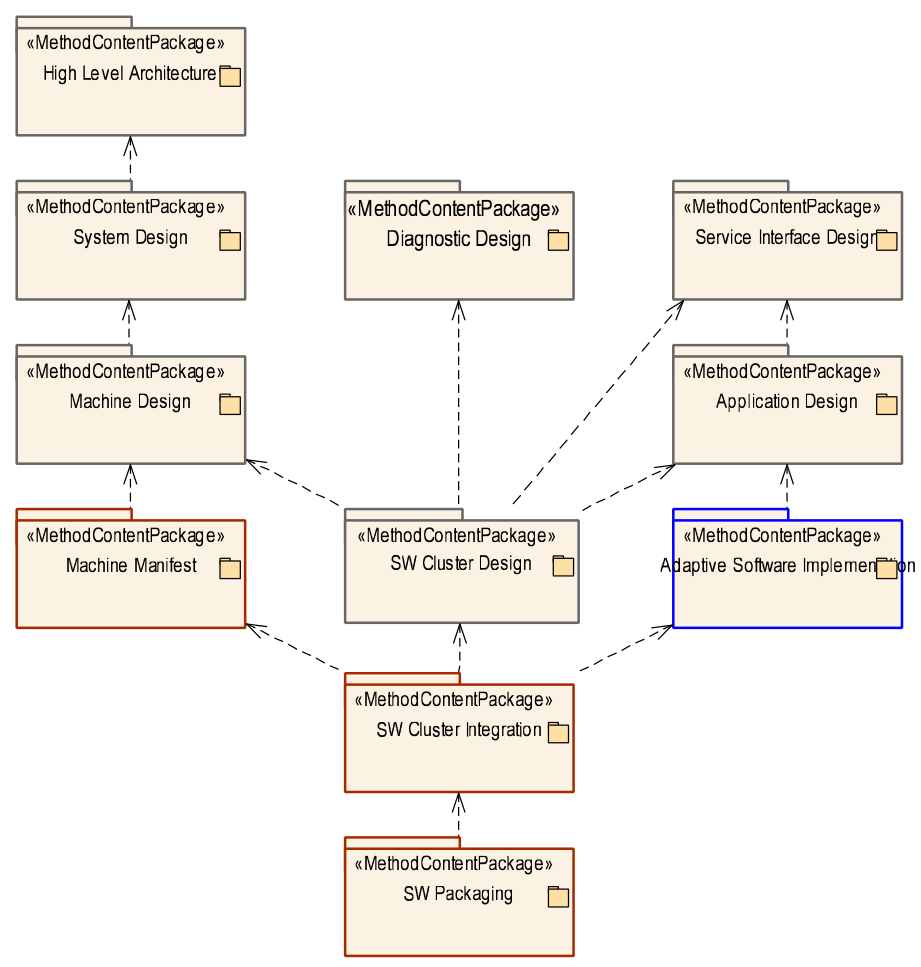
\includegraphics[width=0.75\textwidth]{Images/chap3/image_methodology/knowledgeBase/AdaptiveMethodology.png}
    \vspace{0.5cm}
    \caption{Adaptive Methodology}
    \label{fig:adap_methodology}
\end{figure}

% \subsubsection{High Level Architecture}

% % Figure before explanation
% \begin{figure}[H] % Dùng ht (here, top) là chuẩn nhất
%     \centering
%     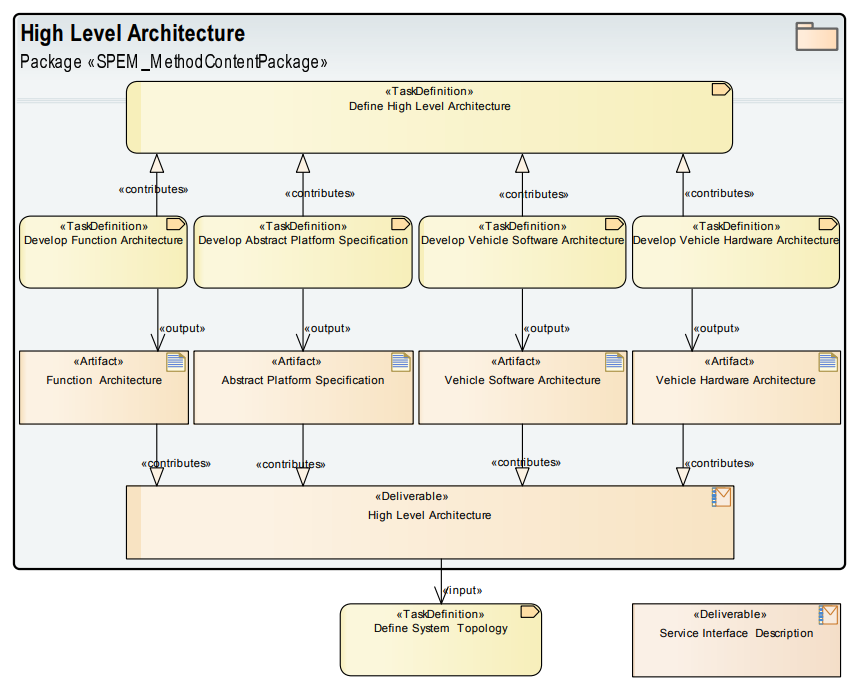
\includegraphics[width=0.75\textwidth]{Images/chap3/image_methodology/knowledgeBase/HLA.png}
%     \vspace{0.5cm}
%     \caption{High Level Architecture in Adaptive AUTOSAR Methodology}
%     \label{fig:hla_architecture} % Đã đổi tên nhãn để không trùng
% \end{figure}

% The High Level Architecture represents the initial and most abstract architectural view within the Adaptive AUTOSAR Methodology. Its primary purpose is to establish a common architectural foundation for the vehicle E/E system before detailed system design and implementation activities are performed.

% As illustrated in Figure~\ref{fig:hla_architecture}, the High Level Architecture is defined through a set of coordinated architectural tasks that collectively contribute to a unified architectural deliverable. These tasks include the development of the Function Architecture, the Abstract Platform Specification, the Vehicle Software Architecture, and the Vehicle Hardware Architecture. Each task addresses a specific architectural concern while remaining independent of concrete implementation decisions.

% The Function Architecture focuses on identifying and structuring the system functions and their logical relationships. It describes what the system is expected to do, without specifying how or where these functions are executed. In parallel, the Abstract Platform Specification defines the abstract execution environment and platform capabilities required by the software, serving as a conceptual bridge between functional requirements and platform realization.

% The Vehicle Software Architecture describes the high level organization of software elements within the vehicle, including major software partitions and their responsibilities. Complementarily, the Vehicle Hardware Architecture captures the high-level hardware structure of the system, including computing units and their relationships, without binding the architecture to specific hardware components.

% The outputs of these architectural tasks are formalized as architectural artefacts. These artefacts collectively contribute to the High-Level Architecture deliverable, which serves as a key input for subsequent methodology phases. In particular, the High Level Architecture provides the architectural context required for defining the system topology and service interface descriptions in later stages.

% By separating functional, software, hardware, and platform concerns at this early stage, the High Level Architecture supports architectural clarity, scalability, and consistency. It ensures that subsequent design and integration activities are grounded in a coherent and well-structured architectural vision.


% \subsubsection{System Design}

% % Figure before explanation
% \begin{figure}[H] % Dùng ht (here, top) là chuẩn nhất
%     \centering
%     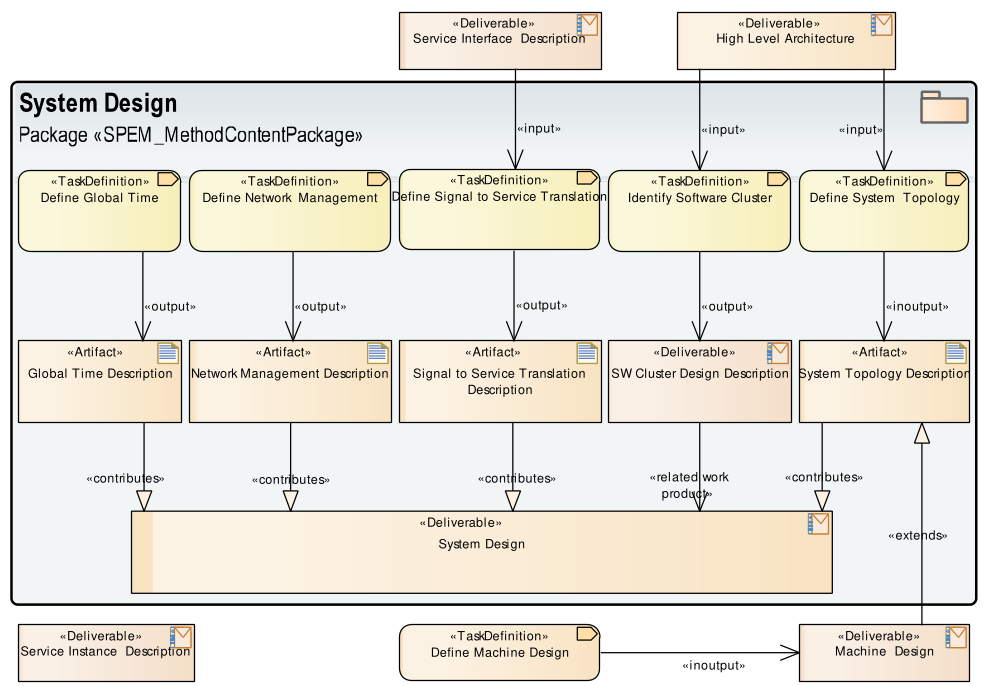
\includegraphics[width=0.75\textwidth]{Images/chap3/image_methodology/knowledgeBase/systemDesign.png}
%     \vspace{0.5cm}
%     \caption{System Design in Adaptive AUTOSAR Methodology}
%     \label{fig:system_design} % Đã đổi tên nhãn để không trùng
% \end{figure}

% The System Design phase refines the architectural concepts established in the High-Level Architecture into a more concrete and structured system-level description. Its primary objective is to define how software elements, communication mechanisms, and system resources are organized and coordinated within the Adaptive AUTOSAR environment.

% As illustrated in the System Design package, this phase consumes key architectural deliverables, including the High Level Architecture and the Service Interface Description, as inputs. Based on these inputs, a set of dedicated design tasks is performed to derive detailed system artefacts that collectively form the System Design deliverable.

% One of the central tasks in this phase is the definition of global timing concepts. The \textit{Define Global Time} task establishes a common time base for the system, which is essential for coordinating distributed software execution and ensuring temporal consistency across different system elements. The resulting Global Time Description contributes to the overall System Design by providing a unified temporal reference.

% In parallel, the \textit{Define Network Management} task specifies how communication networks are controlled and supervised at the system level. This task produces the Network Management Description, which defines network states, transitions, and management strategies. These definitions support reliable communication and controlled system behavior during startup, operation, and shutdown phases.

% Another key task within this phase is the \textit{Define Signal to Service Translation}. This task addresses the mapping between signal-oriented communication and service-oriented communication. The resulting Signal to Service Translation Description enables interaction between system elements that rely on different communication paradigms, ensuring compatibility and interoperability within the Adaptive Platform.

% The System Design phase also includes the identification of software clusters through the \textit{Identify Software Cluster} task. Software clusters group related software elements into coherent deployment units. The resulting Software Cluster Design Description serves as an important intermediate artefact that supports later integration and deployment activities.

% Furthermore, the \textit{Define System Topology} task specifies how system elements are arranged and connected. The System Topology Description captures function groups, network endpoints, and their relationships. This description provides a structural view of the system and serves as a foundation for subsequent deployment and machine-specific design steps.

% All artefacts generated during these tasks contribute to the System Design deliverable. Together, they establish a consistent and detailed system level specification that bridges the gap between high level architectural concepts and later design phases. The System Design deliverable also provides essential inputs for related activities, such as service instance specification and machine design.

% By consolidating timing, communication, clustering, and topology aspects, the System Design phase ensures that the Adaptive AUTOSAR system is coherently structured and ready for further refinement in subsequent methodology stages.


% % TODO: Insert system topology and communication overview figure

% \subsubsection{Service Interface Design}

% % Figure before explanation
% \begin{figure}[H] % Dùng ht (here, top) là chuẩn nhất
%     \centering
%     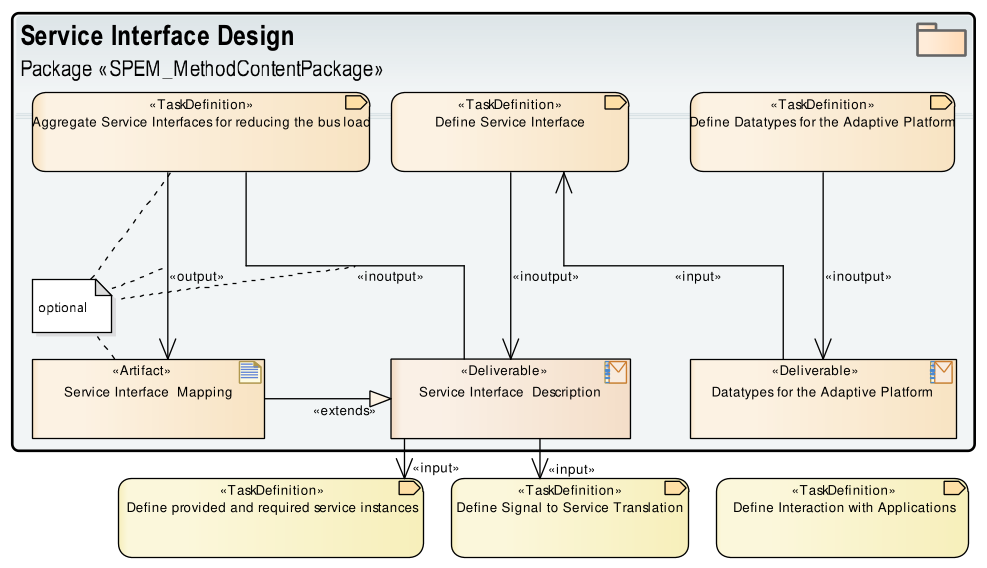
\includegraphics[width=0.75\textwidth]{Images/chap3/image_methodology/knowledgeBase/serviceInterfaceDesign.png}
%     \vspace{0.5cm}
%     \caption{Service Interface Design in Adaptive AUTOSAR Methodology}
%     \label{fig:service_interface_design} % Đã đổi tên nhãn để không trùng
% \end{figure}

% The Service Interface Design defines how Service Interface Descriptions are created, refined, and reused within the Adaptive AUTOSAR development process. This usage scenario explains the sequence of design activities and their associated work products, as illustrated in Figure~\ref{fig:service_interface_design}, focusing on the relationship between service interfaces, datatypes, and interface mappings.

% According to the methodology, Service Interface Descriptions can be obtained through two main usage scenarios: create or change use cases and reuse use cases. These scenarios are not isolated phases but can be integrated into both system design and application design activities, depending on the development context.

% In create or change use cases, Service Interface Descriptions are derived by performing a set of tailored tasks. The central task is the definition of a service interface, which specifies the service operations, events, and communication semantics. In parallel, datatypes for the Adaptive Platform are defined or refined to describe the data exchanged through the service interface. These tasks may be supported by the aggregation of service interfaces, which aims to reduce communication bus load by grouping related service elements when appropriate. The resulting Service Interface Mapping artefact optionally extends the Service Interface Description by documenting how aggregated or related interfaces are organized.

% This scenario is typically applied in a top-down development approach, where architectural or system level considerations drive the definition of service interfaces and datatypes. The outputs of these tasks include the Service Interface Description and the Datatypes for the Adaptive Platform, which together form the primary deliverables of this design stage.

% In reuse use cases, existing Service Interface Descriptions are adopted as inputs with minimal modification. In this case, service interfaces and their associated datatypes are reused from predefined specifications or existing libraries. If required, datatypes may be extended to align with the specific system context. This scenario is commonly applied in a bottom-up development approach and supports efficient reuse across different projects.

% The resulting work products of both scenarios are tailored Service Interface Descriptions and corresponding Datatype Descriptions. These deliverables serve as inputs for subsequent design activities, such as the definition of provided and required service instances, signal-to-service translation, and the specification of interactions with applications.

% By explicitly structuring the creation, aggregation, mapping, and reuse of service interfaces, the Service Interface Design usage scenario ensures consistency, modularity, and reusability of service definitions within the Adaptive AUTOSAR methodology.

% \subsubsection{Application Design}

% % Figure before explanation
% \begin{figure}[H]
%     \centering
%     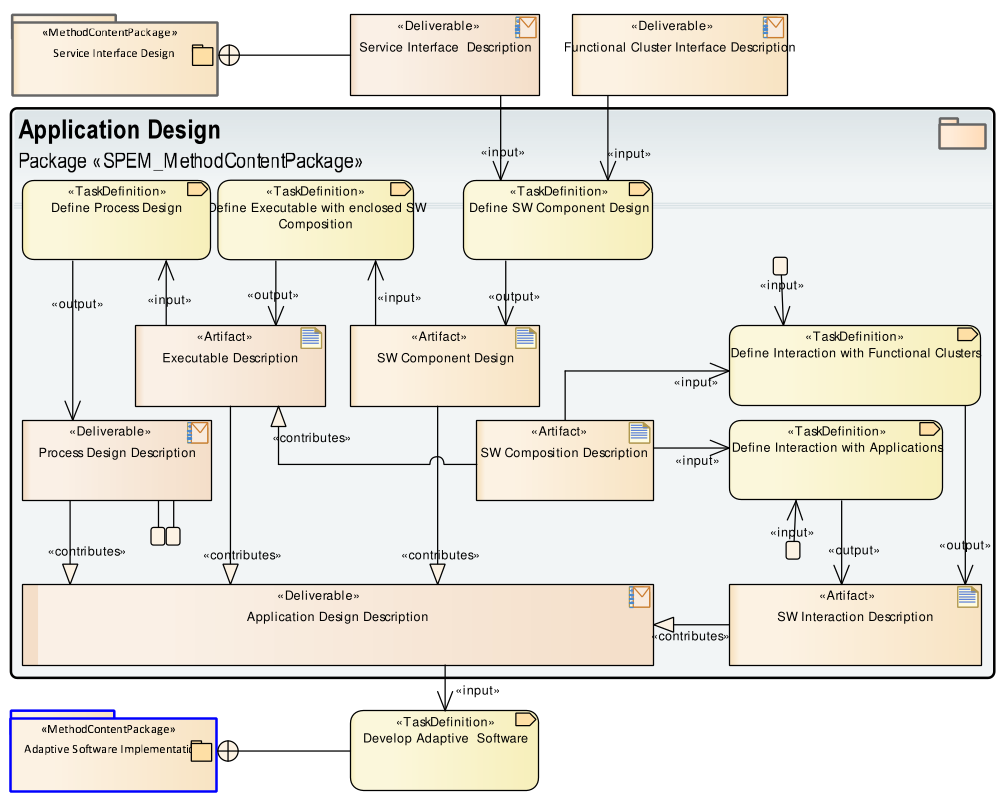
\includegraphics[width=0.75\textwidth]{Images/chap3/image_methodology/knowledgeBase/applicationDesign.png}
%     \vspace{0.5cm}
%     \caption{Application Design in Adaptive AUTOSAR Methodology}
%     \label{fig:application_design}
% \end{figure}

% The Application Design phase refines the outcomes of system level and service-level design into a detailed specification of executable software structures. Its primary objective is to describe how software components are organized, instantiated, and interconnected during runtime execution within the Adaptive AUTOSAR Platform.

% As shown in Figure~\ref{fig:application_design}, this phase takes the Service Interface Description and the Functional Cluster Interface Description as inputs. Based on these artefacts, a set of closely related design activities is carried out, leading to the definition of the overall Application Design Description.

% One of the key activities in this phase is \textit{Define Software (SW) Component Design}. This activity results in the SW Component Design artefact, which specifies the internal structure of software components and their interaction endpoints. These endpoints are expressed through software component (SWC) ports instantiating specific port interfaces at either the application level or the platform level. The SW Component Design establishes the structural basis required for subsequent composition and interaction definitions.

% Another essential activity is \textit{Define Executable with enclosed SW Composition}, which determines how software components are assembled into executable units. Its outcome is the Executable Description, including the SW Composition Description. This description identifies the software components contained within an executable and defines their structural relationships. The execution of this activity requires that all referenced SW Component Designs are already available.

% The runtime realization of executables is addressed by the \textit{Define Process Design} activity. The resulting Process Design Description represents a design time abstraction of the operating system process responsible for instantiating and starting a specific executable. This activity builds upon the Executable Description and provides the link between executable definitions and their runtime execution context.

% Interaction which related aspects are specified through the activities \textit{Define Interaction with Applications} and \textit{Define Interaction with Functional Clusters}. Together, these activities produce the SW Interaction Description, which captures all interaction configurations that are relevant at design time. This includes interactions between application-level software components as well as interactions with platform-level functional clusters. The definition of these interactions depends on the availability of the Process Design Description, the corresponding Executable Description with its SW Composition Description, and the interaction endpoints defined in the SW Component Designs.

% All artefacts produced during the Application Design phase contribute to the Application Design Description deliverable. This deliverable consolidates software component definitions, executable compositions, process abstractions, and interaction configurations into a consistent and comprehensive design representation.

% The activities within the Application Design phase are interdependent and may be performed in an order that best fits the project context. Although the primary focus of this phase is on application-level software, the same design principles and activities may also be applied to platform-level software, particularly when port and port interface concepts are supported.

% The resulting Application Design Description serves as a fundamental input for the subsequent Adaptive Software Implementation phase, where the defined software structures are realized as executable software.

% \subsubsection{Adaptive Software Implementation}

% % Figure before explanation
% \begin{figure}[H]
%     \centering
%     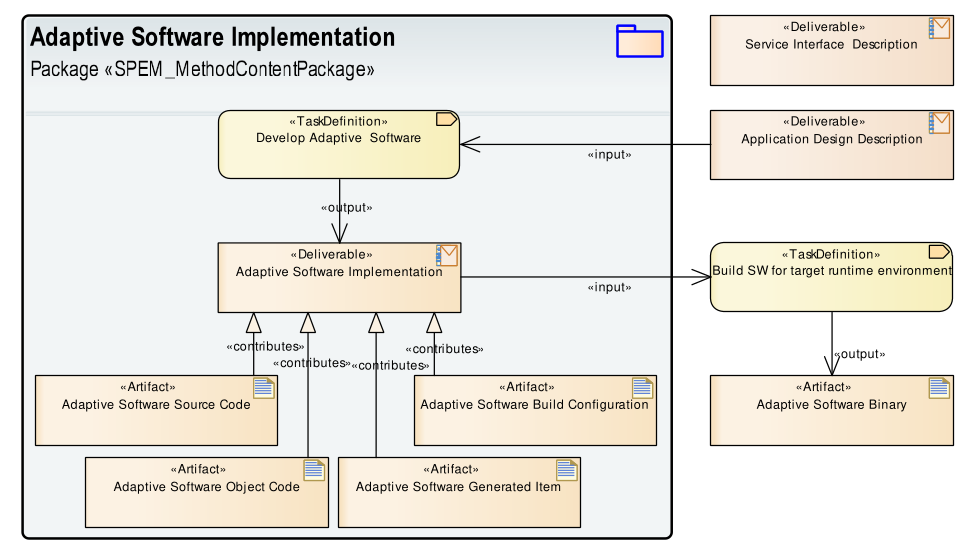
\includegraphics[width=0.75\textwidth]{Images/chap3/image_methodology/knowledgeBase/softwareImplementation.png}
%     \vspace{0.5cm}
%     \caption{Adaptive Software Implementation in Adaptive AUTOSAR Methodology}
%     \label{fig:software_implementation}
% \end{figure}

% The Adaptive Software Implementation phase addresses the realization of software defined during the preceding design stages. Its purpose is to transform the Application Design Description into concrete software artefacts that can be integrated and executed within the Adaptive AUTOSAR runtime environment.

% As depicted in Figure~\ref{fig:software_implementation}, this phase is initiated once the Service Interface Description and the Application Design Description are available. These deliverables provide the necessary interface definitions and structural specifications required to start the implementation activities.

% The central activity of this phase is \textit{Develop Adaptive Software}. This activity encompasses the development of application level and/or platform level Adaptive Software and may include analysis, detailed design, implementation, and testing activities. The development process relies on Adaptive Software Generated Items, such as service proxies and service skeletons, which are derived from service interface definitions and support the implementation of communication ports and port interfaces.

% Depending on the availability of the Adaptive Software Build Configuration, the development process follows different realization paths. When the build configuration is known in advance, software components can be compiled by the developer, and Adaptive Software Object Code can be delivered directly. In contrast, if the build configuration is not available, the developer provides Adaptive Software Source Code, and the compilation is performed later by the integrator.

% The artefacts produced during software development include Adaptive Software Source Code, Adaptive Software Object Code, Adaptive Software Generated Items, and the Adaptive Software Build Configuration. Together, these artefacts contribute to the Adaptive Software Implementation deliverable, which represents the complete implementation result prepared for integration.

% The transformation of the implementation into deployable form is addressed by the activity \textit{Build software (SW) for target runtime environment}. This activity consumes the Adaptive Software Implementation and produces the Adaptive Software Binary. The binary represents the executable form of the software that is suitable for deployment on the target machine and runtime environment.

% Throughout this phase, both application level and platform level Adaptive Software are treated consistently. Each executable requires a main function and an execution manifest, enabling instantiation and deployment within the Adaptive AUTOSAR execution framework.

% The Adaptive Software Implementation deliverable produced in this phase serves as the handover point between software development and integration. It provides the necessary implementation artefacts for subsequent software cluster integration, packaging, and deployment activities.

% \subsubsection{Diagnostic Design}

% % Figure before explanation
% \begin{figure}[H]
%     \centering
%     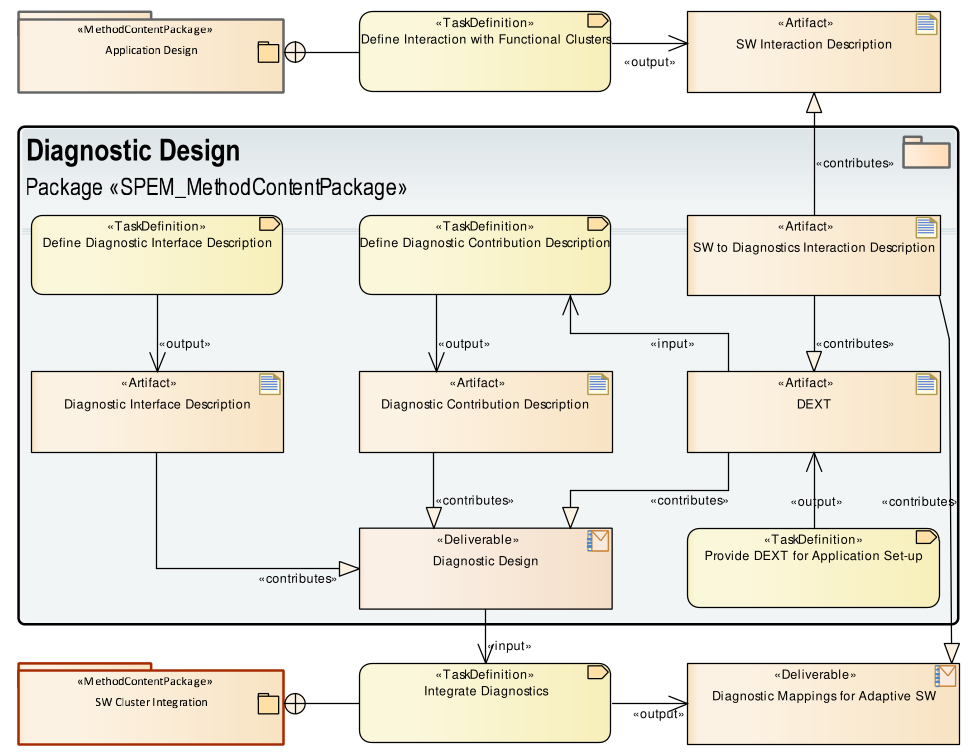
\includegraphics[width=0.75\textwidth]{Images/chap3/image_methodology/knowledgeBase/diagDesign.png}
%     \vspace{0.5cm}
%     \caption{Diagnostic Design in Adaptive AUTOSAR Methodology}
%     \label{fig:diag_design}
% \end{figure}

% The Diagnostic Design phase focuses on defining how diagnostic information is associated with the software structures of the Adaptive AUTOSAR system. Its main objective is to prepare diagnostic which related artefacts that enable consistent monitoring, reporting, and interaction with the diagnostic manager during system operation.

% As shown in Figure~\ref{fig:diag_design}, Diagnostic Design builds on results obtained during the Application Design phase, particularly the SW Interaction Description that captures interactions with functional clusters. These interaction definitions provide the context required to specify diagnostic interfaces and mappings in a systematic manner.

% The activity \textit{Define Diagnostic Interface Description} establishes the diagnostic interfaces that adaptive software components expose for diagnostic purposes. The resulting Diagnostic Interface Description specifies diagnostic port interfaces and their characteristics, allowing diagnostic managers to access diagnostic which relevant data and services in a standardized way.

% Complementing this, the activity \textit{Define Diagnostic Contribution Description} identifies the diagnostic content contributed by software elements within a given context. The Diagnostic Contribution Description determines which parts of the diagnostic configuration are relevant for specific executables or software clusters and are intended to be processed by the diagnostic manager.

% Diagnostic resources and configuration data are collected and structured through the activity \textit{Provide DEXT for Application Setup}. This activity produces or extends the Diagnostic Extract (DEXT), which contains diagnostic resources such as diagnostic data identifiers, diagnostic events, enable conditions, and operation cycles. The DEXT acts as a reusable container for diagnostic configuration and may cover multiple executables, diagnostic managers, and software clusters across the vehicle.

% The association between diagnostic resources and software interaction endpoints is captured in the SW to Diagnostics Interaction Description. This artefact specifies how diagnostic information is mapped to software component ports at design time and contributes both to the Diagnostic Design deliverable and to the DEXT. It represents an intermediate form of diagnostic mappings that is refined during later integration steps.

% All artefacts produced during this phase, including the Diagnostic Interface Description, Diagnostic Contribution Description, SW to Diagnostics Interaction Description, and the DEXT, collectively contribute to the Diagnostic Design deliverable. This deliverable provides a consolidated view of the diagnostic configuration that is prepared for further integration activities.

% The Diagnostic Design deliverable is subsequently used as input for the \textit{Integrate Diagnostics} activity during Software Cluster Integration. In that phase, diagnostic mappings are finalized by associating diagnostic resources with concrete executable instances and operating system processes, resulting in the Diagnostic Mappings for Adaptive Software.

% By structuring diagnostic interface definition, contribution specification, and resource extraction as distinct but related activities, the Diagnostic Design phase supports a clear and maintainable diagnostic configuration process within the Adaptive AUTOSAR methodology.

% \subsubsection{Machine Design}

% % Figure before explanation
% \begin{figure}[H]
%     \centering
%     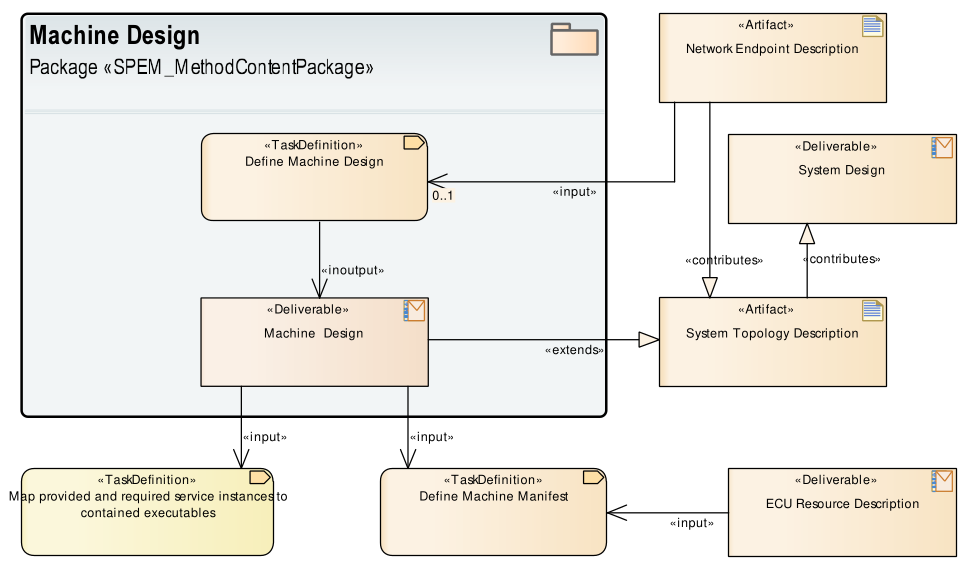
\includegraphics[width=0.75\textwidth]{Images/chap3/image_methodology/knowledgeBase/machineDesign.png}
%     \vspace{0.5cm}
%     \caption{Machine Design in Adaptive AUTOSAR Methodology}
%     \label{fig:machine_design}
% \end{figure}

% The Machine Design phase addresses the specification of a machine from a communication and deployment standpoint within the Adaptive AUTOSAR Platform. Its aim is to describe the characteristics of a machine that are required for software execution and service communication, taking into account system level topology information and the capabilities of the target ECU.

% Figure~\ref{fig:machine_design} provides an overview of the activities involved in this phase. The core activity, \textit{Define Machine Design}, derives a machine-oriented configuration by using network endpoint information defined during System Design. In particular, the System Topology Description and the associated Network Endpoint Description supply the addressing and service discovery parameters needed to shape the communication behavior of the machine.

% The result of this activity is captured in the Machine Design deliverable. This deliverable augments the existing System Topology Description by introducing machine specific communication constraints and requirements. At this stage, the design remains independent of a concrete hardware realization and represents a prospective configuration for a machine.

% Beyond defining communication aspects, the Machine Design also provides the basis for associating software deployment elements with the machine. Through the activity \textit{Map provided and required service instances to contained executables}, service instances are linked to executables that are intended to run on the machine. This association clarifies how services are realized by software units within the machine context.

% The adaptation of the machine configuration to a specific hardware platform is performed in a subsequent activity, \textit{Define Machine Manifest}. This activity combines the Machine Design with the ECU Resource Description, which details the resources and limitations of the target ECU. The outcome is the Machine Manifest, representing a machine configuration that is fully aligned with the characteristics of a real ECU.

% From a methodological viewpoint, machine configuration follows a two-step process. The first step establishes the communication structure of a machine and yields the Machine Design. This step may be carried out in a top-down manner, guided by an existing System Design, or in a bottom-up manner, where machine-specific communication definitions are created locally and may later contribute to the overall system topology.

% The second step focuses on hardware-specific realization and results in the Machine Manifest. This separation between prospective machine definition and ECU specific configuration supports a clear allocation of responsibilities between system designers and integrators, while maintaining flexibility during system integration.

% \subsubsection{Machine Manifest}

% % Figure before explanation
% \begin{figure}[H]
%     \centering
%     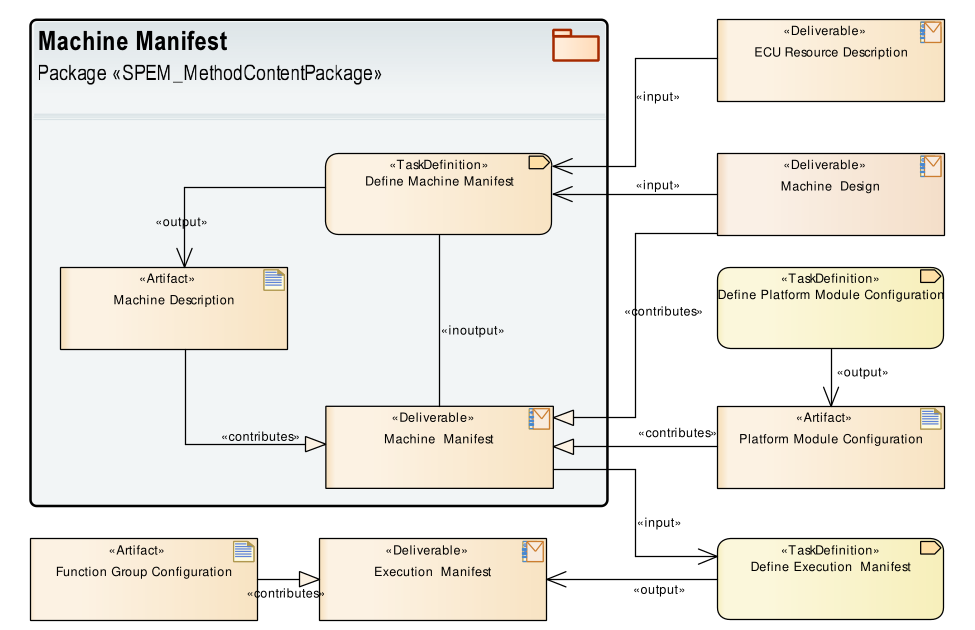
\includegraphics[width=0.75\textwidth]{Images/chap3/image_methodology/knowledgeBase/machineManifest.png}
%     \vspace{0.5cm}
%     \caption{Machine Manifest in Adaptive AUTOSAR Methodology}
%     \label{fig:machine_manifest}
% \end{figure}

% The Machine Manifest phase specifies the final configuration of a machine that is ready to be deployed on a concrete ECU within the Adaptive AUTOSAR Platform. Its purpose is to consolidate communication-related design results with hardware resource information and platform-specific configurations into a single, deployment ready description.

% Figure~\ref{fig:machine_manifest} outlines the activities and work products involved in this phase. The primary activity, \textit{Define Machine Manifest}, is initiated once the Machine Design and the ECU Resource Description are available. While the Machine Design provides a prospective view of the machine configuration, the ECU Resource Description defines the concrete hardware resources offered by the target ECU.

% The outcome of this activity is the Machine Manifest deliverable. The Machine Manifest integrates several key elements. First, it contains the Machine Description, which describes the available hardware resources of the ECU, such as processing units, memory resources, sensors, actuators, and other relevant hardware elements. This information is derived from the ECU Resource Description and tailored to the specific machine instance.

% Second, the Machine Manifest incorporates the Machine Design, thereby preserving the communication structure and network-related configuration that was defined during the Machine Design phase. This ensures that the communication requirements identified earlier are consistently realized on the target ECU.

% In addition, platform-specific aspects are addressed through the activity \textit{Define Platform Module Configuration}. This activity produces Platform Module Configuration artefacts, which specify the machine-specific configuration of Adaptive Platform modules. These configurations may include the operating system setup, platform services such as network management and diagnostics, as well as foundation modules like logging and tracing. The resulting Platform Module Configurations contribute directly to the Machine Manifest.

% The configuration of software execution is captured by the activity \textit{Define Execution Manifest}. This activity produces the Execution Manifest, which specifies which executables are instantiated on the machine and how they are mapped to processes. The Execution Manifest may also include Function Group Configurations that control the activation and deactivation of software elements. The Execution Manifest contributes to the Machine Manifest by defining the runtime behavior of software on the machine.

% From a process perspective, the Machine Manifest is typically assembled in an incremental manner. Communication-related configurations originating from the Machine Design are collected first, followed by the integration of hardware resource descriptions and platform module configurations. As additional configuration information becomes available, the Machine Manifest may be iteratively extended and refined.

% By consolidating machine-specific communication settings, hardware resource descriptions, platform module configurations, and execution information, the Machine Manifest provides a complete and consistent representation of a machine that is ready for deployment within the Adaptive AUTOSAR ecosystem.

% \subsubsection{Software Cluster Design, Integration, and Packaging}

% The phases of Software Cluster Design, Software Cluster Integration, and Software Packaging together form the final preparation steps that transform implemented Adaptive AUTOSAR software into deployable units. These phases consolidate design results, integrate software components with their configurations, and prepare complete software packages for deployment on target machines.

% Software Cluster Design focuses on defining logical groupings of software elements that belong together from a deployment and lifecycle perspective. A software cluster typically bundles application level software, required platform services, and related configuration artifacts into a coherent unit. The purpose of this phase is not to define execution details, but to establish clear cluster boundaries, dependencies, and responsibilities that simplify later integration and deployment activities.

% Based on the cluster definitions, Software Cluster Integration performs the concrete assembly of software and configuration artifacts. During this phase, Adaptive Software Implementations, design descriptions, machine which related information, and diagnostic configurations are brought together and checked for consistency. Integration activities refine execution which related information, such as the association of executables with machines and processes, and complete interaction and diagnostic mappings that could only be finalized once all involved elements are known. As a result, the integrated software cluster represents a consistent and executable view of the system for a specific deployment context.

% Software Packaging completes the workflow by preparing integrated software clusters for delivery and deployment. In this phase, all relevant artifacts, such as software binaries, manifests, configuration files and generated items which are collected and organized into software packages. These packages are structured in a way that supports deployment, update, and lifecycle management, while preserving a clear separation between different software clusters.

% By combining cluster definition, integration, and packaging into a structured workflow, these phases provide a clear transition from implemented software to deployable units. This approach supports modularity, reuse, and scalable integration, which are essential characteristics of the Adaptive AUTOSAR methodology.

% \subsubsection{Summary}

% This section has presented an overview of the Adaptive AUTOSAR knowledge base and its role in structuring the development of complex automotive software systems. The methodology defines a clear sequence of development phases, each supported by well-defined artefacts and responsibilities.

Starting from high-level architectural descriptions, the methodology guides the refinement of system structure, service interfaces, application design, and software implementation. Subsequent phases address diagnostics, machine-specific configuration, and the preparation of software for deployment. Each phase builds upon the results of previous stages, ensuring consistency and traceability throughout the development process.

By explicitly modeling artefact dependencies and separating design, implementation, integration, and deployment concerns, the Adaptive AUTOSAR Methodology supports systematic system development. This approach improves scalability, facilitates reuse, and simplifies integration in large and evolving software systems.

The following section explains how the most important Method Content Packages are configured in this project and how they are refined into concrete Adaptive AUTOSAR artefacts.

% Overall, the knowledge base provides a solid methodological foundation for configuring and deploying Adaptive AUTOSAR systems. It enables a structured transition from abstract system concepts to deployable software units while maintaining clarity and consistency across the entire system lifecycle.


\subsection{Project Methodology}

In this project, the Adaptive AUTOSAR system is developed using the \texttt{Autosar.io} tool provided by PopcornSAR. Autosar.io is a configuration-oriented modeling environment that allows users to systematically define and organize an Adaptive AUTOSAR project through a set of well-structured design sections. Instead of focusing on source code implementation, the tool guides users to configure machines, services, and applications by following the standard Adaptive AUTOSAR modeling workflow.

\begin{figure}[H]
    \centering
    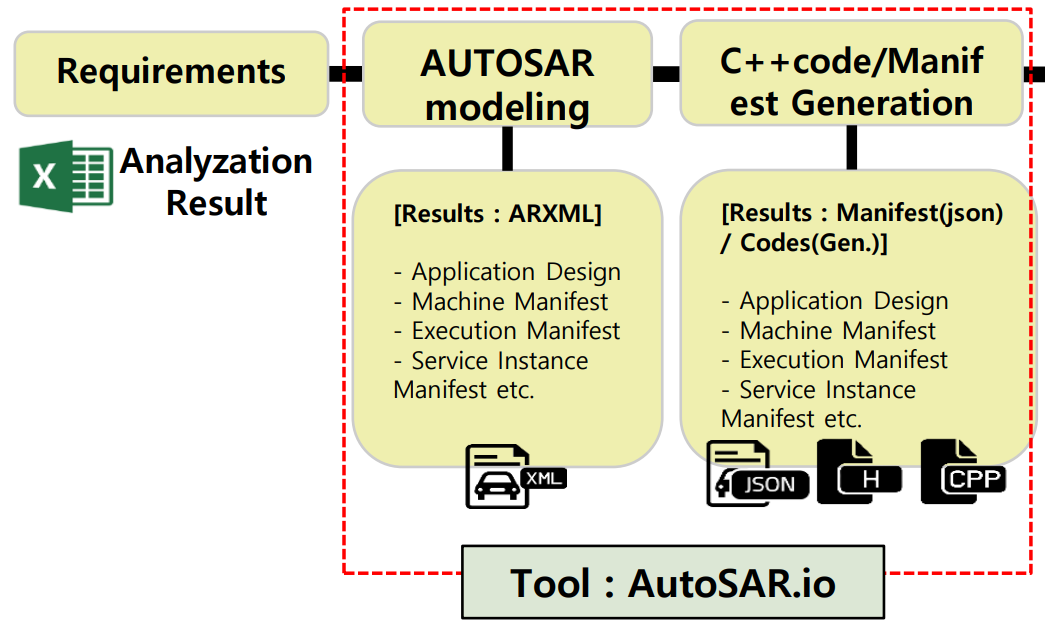
\includegraphics[width=0.75\textwidth]{Images/toolchains/autosario.png}
    \vspace{0.5cm}
    \caption{Autosar.io tool supporting configuration workflow for Adaptive AUTOSAR systems}
    \label{fig:autosario}
\end{figure}

Autosar.io provides dedicated design views that correspond directly to the configuration steps presented in this section, including Machine Design and Machine Manifest creation, Service Interface Design and Mapping, and Adaptive Application Design. Through these views, users can specify network endpoints, service discovery parameters, service interfaces, service instances, application executables, processes, startup behavior, and process-to-machine mappings. Each configuration step produces AUTOSAR-compliant artifacts such as ARXML descriptions and manifests, ensuring consistency between design intent and deployment configuration.

By using Autosar.io, users can incrementally build the system configuration in a top-down manner, where abstract architectural decisions are progressively refined into concrete runtime configurations. This approach enables clear separation between machine-level configuration, service-level communication design, and application-level deployment. As demonstrated throughout this section, Autosar.io acts as the central tool that connects all configuration stages, allowing users to define a complete Adaptive AUTOSAR system in a structured, traceable, and standardized way before moving to implementation and integration phases.

%introduce Autosar.io tool, this is a tool help configuring project based on Adaptive AUTOSAR
\subsubsection{High Level Architecture}
\begin{figure}[H]
    \centering
    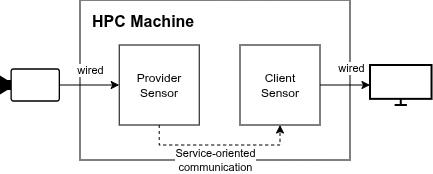
\includegraphics[width=0.75\textwidth]{Images/chap3/image_methodology/machineDesign/high_level.png}
    \vspace{0.5cm}
    \caption{High Level Architecture of Prototype Project}
    \label{fig:hla_project}
\end{figure}

Based on the defined high-level architecture, the Adaptive AUTOSAR configuration process is carried out in a stepwise manner, following the recommended methodology. The overall system design is progressively refined from an abstract architectural view to concrete deployment and execution artifacts.

First, the Machine Design and Machine Manifest are configured to define the physical execution environment of the system. This step specifies the target machine, network interfaces, service discovery settings, operating system platform modules, and lifecycle-related parameters, forming the foundation on which all applications and services are deployed.

Next, the Service Interface Design and Mapping phase focuses on defining the service-oriented communication between applications. During this stage, data types, service interfaces, service instances, and deployment configurations are specified, and abstract service definitions are bound to concrete network endpoints. This step enables standardized and loosely coupled interaction between the Provider Sensor and Client Sensor.

Finally, the Application Design phase models the adaptive applications themselves. Executables are defined and configured, ports are mapped to service interfaces, application processes are created, and startup and lifecycle behaviors are specified. Through this step, the logical application design is concretely mapped onto the target machine, completing the system configuration prior to code and manifest generation.

\subsubsection{Machine Design and Machine Manifest}

% Define Ethernet network endpoint
\begin{figure}[H]
    \centering
    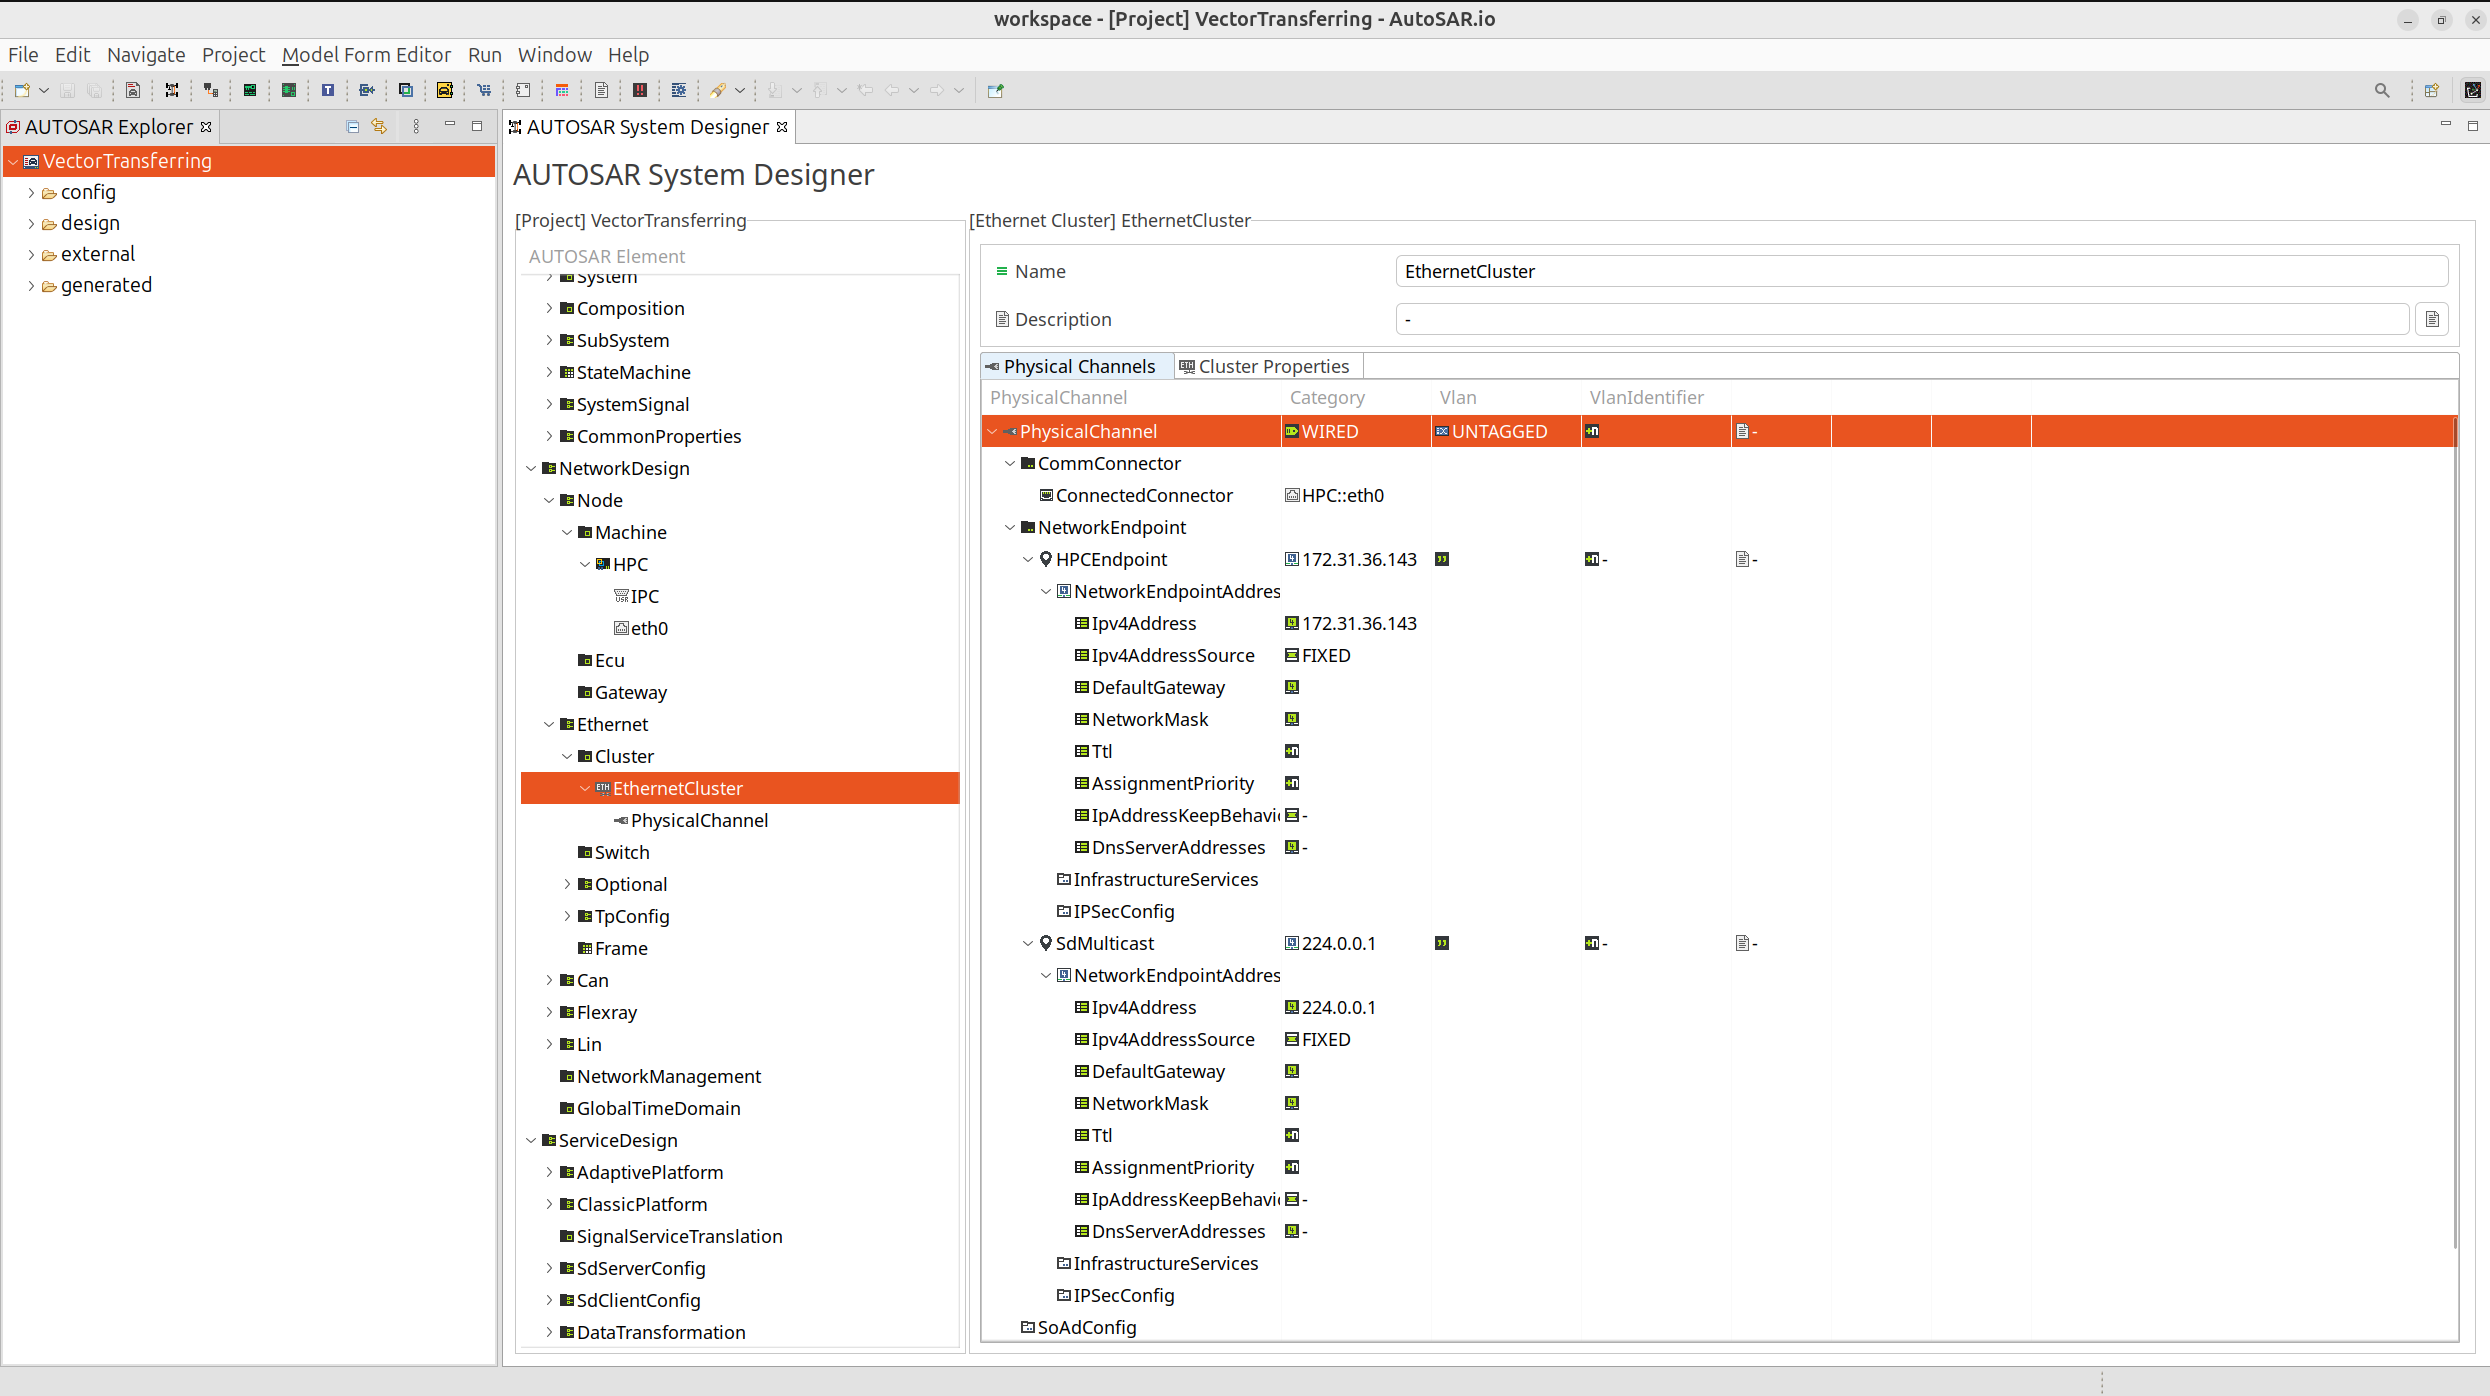
\includegraphics[width=0.75\textwidth]{Images/chap3/image_methodology/machineDesign/defineEthernet.png}
    \vspace{0.5cm}
    \caption{Definition of Ethernet Network Endpoint in Machine Design}
    \label{fig:machine_define_ethernet}
\end{figure}

Figure~\ref{fig:machine_define_ethernet} illustrates the detailed configuration of an Ethernet network endpoint within the AUTOSAR System Designer. An EthernetCluster is defined with a wired physical channel, where the VLAN mode is set to untagged, indicating that no VLAN identifier is applied to the network traffic. The machine node labeled HPC is connected to this cluster through the communication connector HPC eth0, which represents the physical Ethernet interface of the target machine.

The network endpoint configuration specifies a fixed IPv4 address of 172.31.36.143, with the address source explicitly defined as fixed to ensure deterministic network behavior. In addition to the unicast endpoint, a multicast configuration is also present using the IPv4 address 224.0.0.1, which is commonly used for service discovery communication. These settings collectively define how the machine participates in both point to point and multicast Ethernet communication, forming a stable networking foundation for Adaptive AUTOSAR service based applications.

% Add Ethernet configuration to Machine Design
\begin{figure}[H]
    \centering
    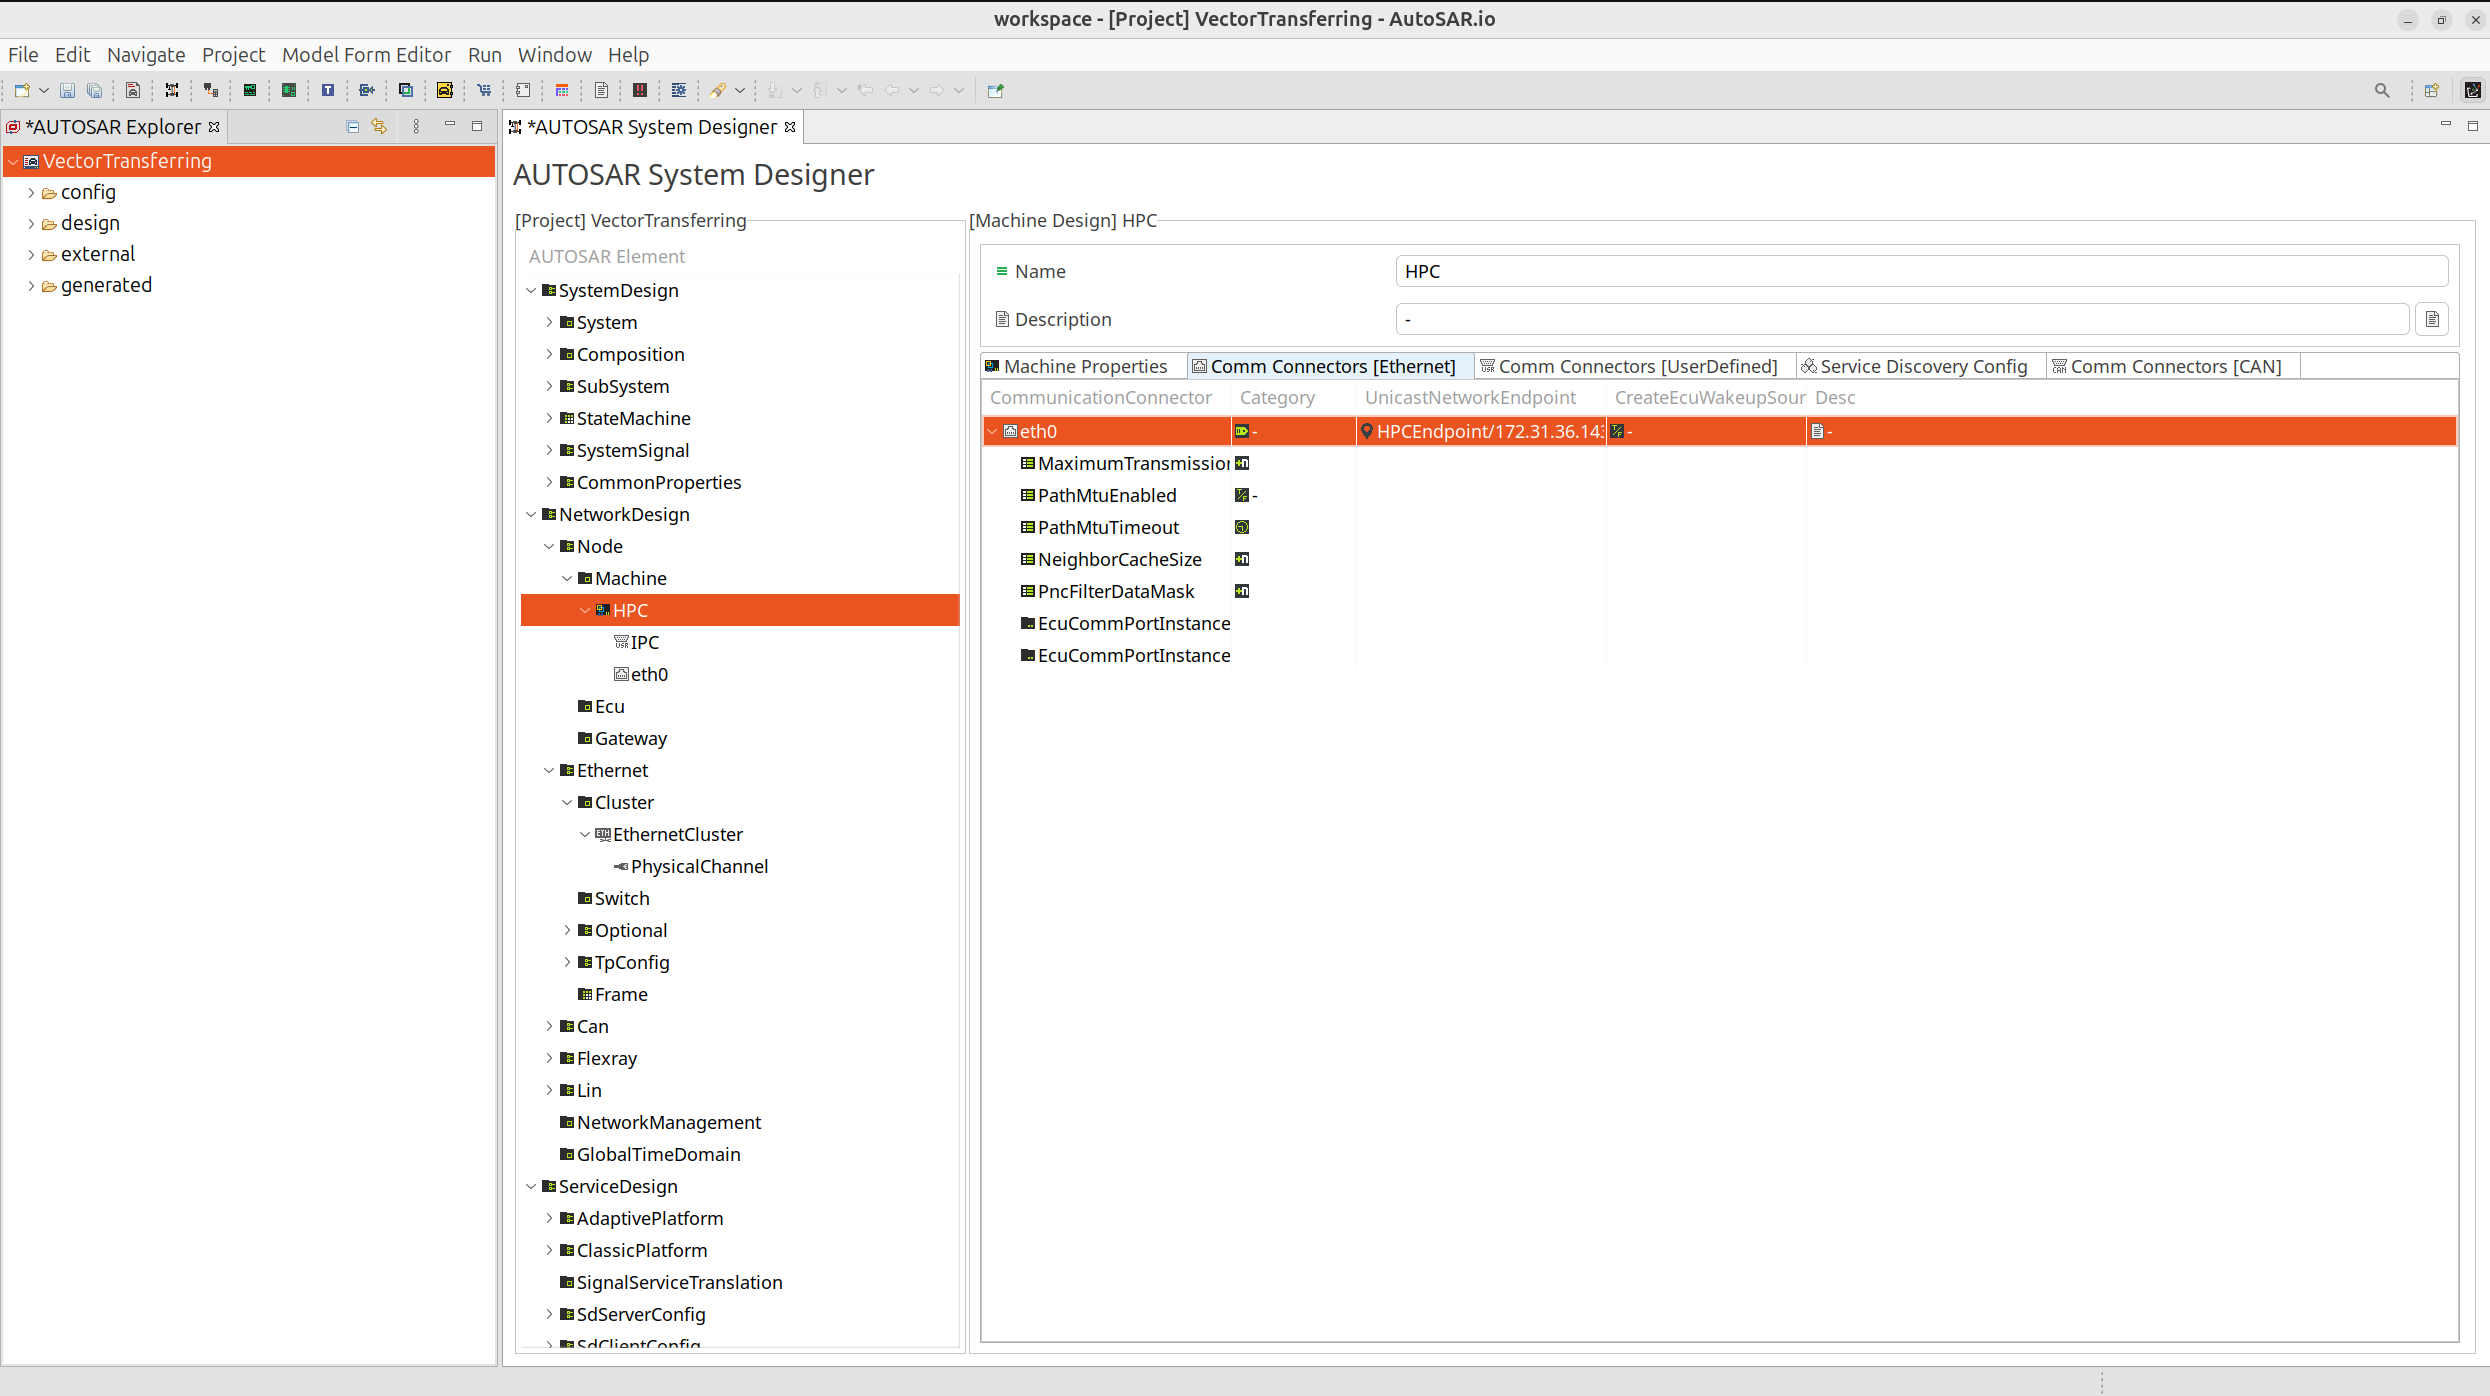
\includegraphics[width=0.75\textwidth]{Images/chap3/image_methodology/machineDesign/addEthMachineDesign.png}
    \vspace{0.5cm}
    \caption{Integration of Ethernet Configuration into Machine Design}
    \label{fig:machine_add_eth_design}
\end{figure}

Figure~\ref{fig:machine_add_eth_design} depicts how the HPC machine is linked to its network interface through the eth0 connector in the Machine Design view. This connector is mapped to a unicast endpoint identified as HPCEndpoint with the IPv4 address 172.31.36.143, defining the machine’s network presence within the Adaptive AUTOSAR system. The figure also highlights adjustable communication parameters such as transmission limits and path MTU handling, which allow the network behavior to be adapted while maintaining reliable data exchange at runtime.

% Configure Service Discovery in Machine Design
\begin{figure}[H]
    \centering
    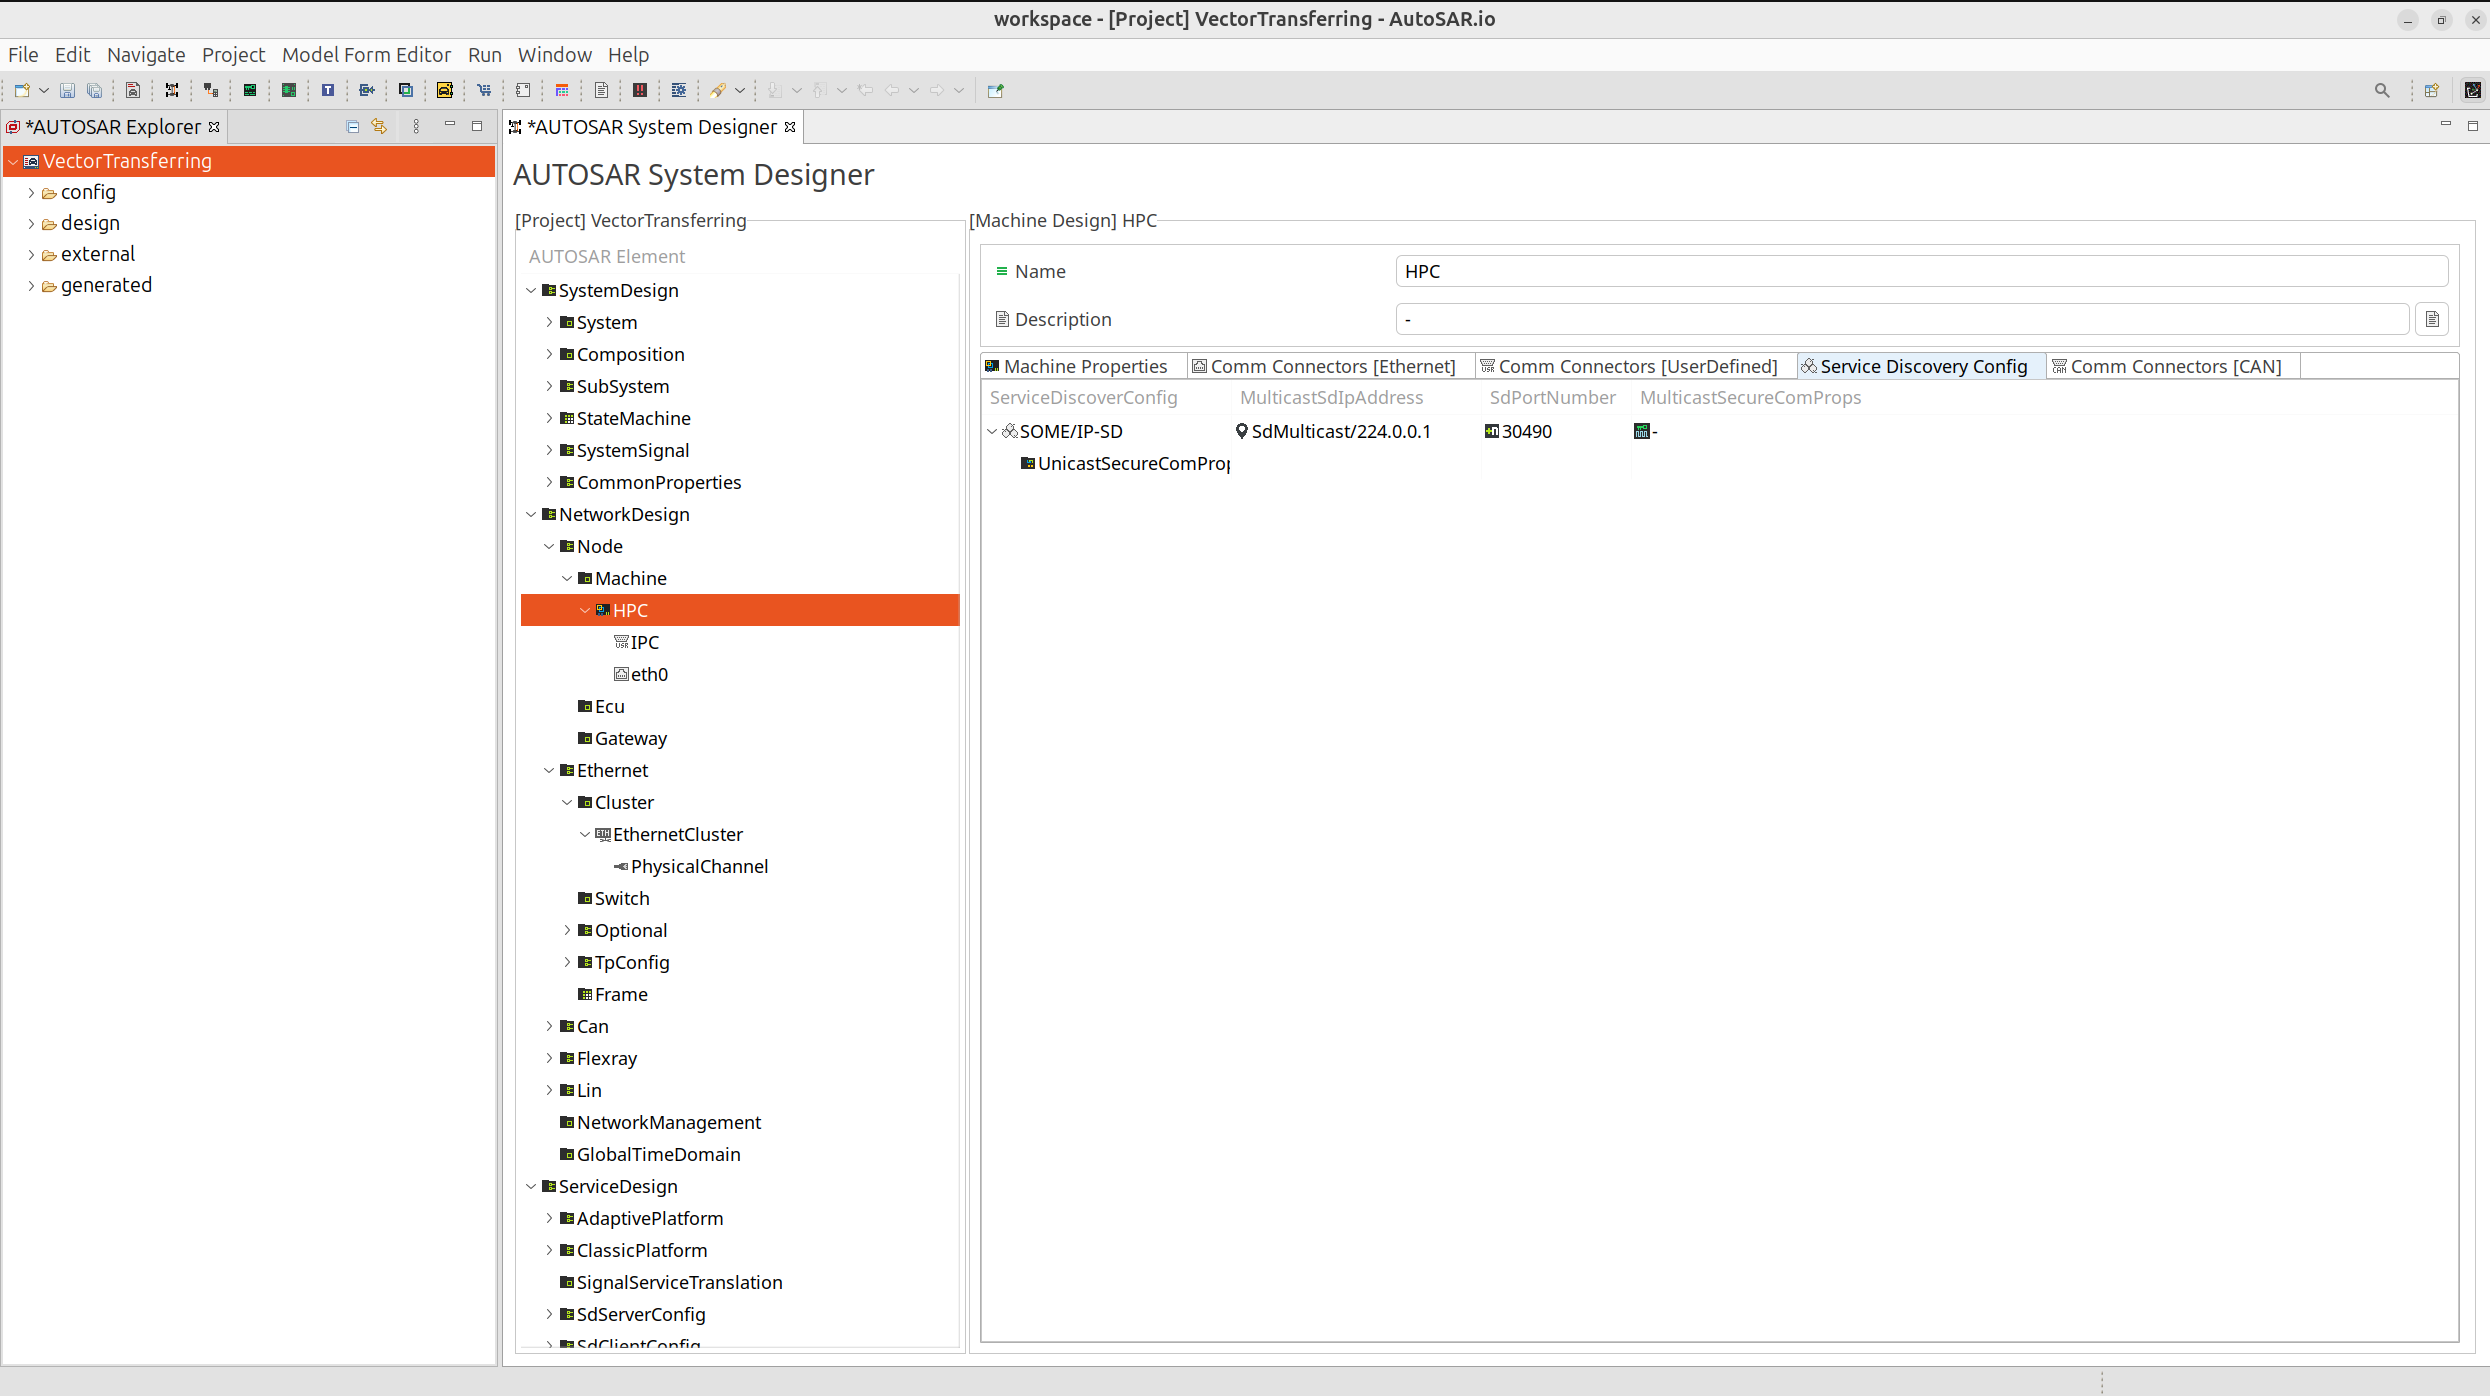
\includegraphics[width=0.75\textwidth]{Images/chap3/image_methodology/machineDesign/addSdConfigMachineDesign.png}
    \vspace{0.5cm}
    \caption{Service Discovery Configuration in Machine Design}
    \label{fig:machine_sd_config}
\end{figure}

Figure~\ref{fig:machine_sd_config} illustrates the Service Discovery setup for the HPC machine within the Machine Design environment. The SOME IP Service Discovery mechanism is configured using the multicast address 224.0.0.1 together with the service discovery port number 30490, which enables applications to announce and detect available services at runtime. This configuration allows dynamic interaction between Adaptive AUTOSAR applications while supporting flexible service availability without relying on static communication bindings.

% Configure Diagnostic Log and Trace (DLT)
\begin{figure}[H]
    \centering
    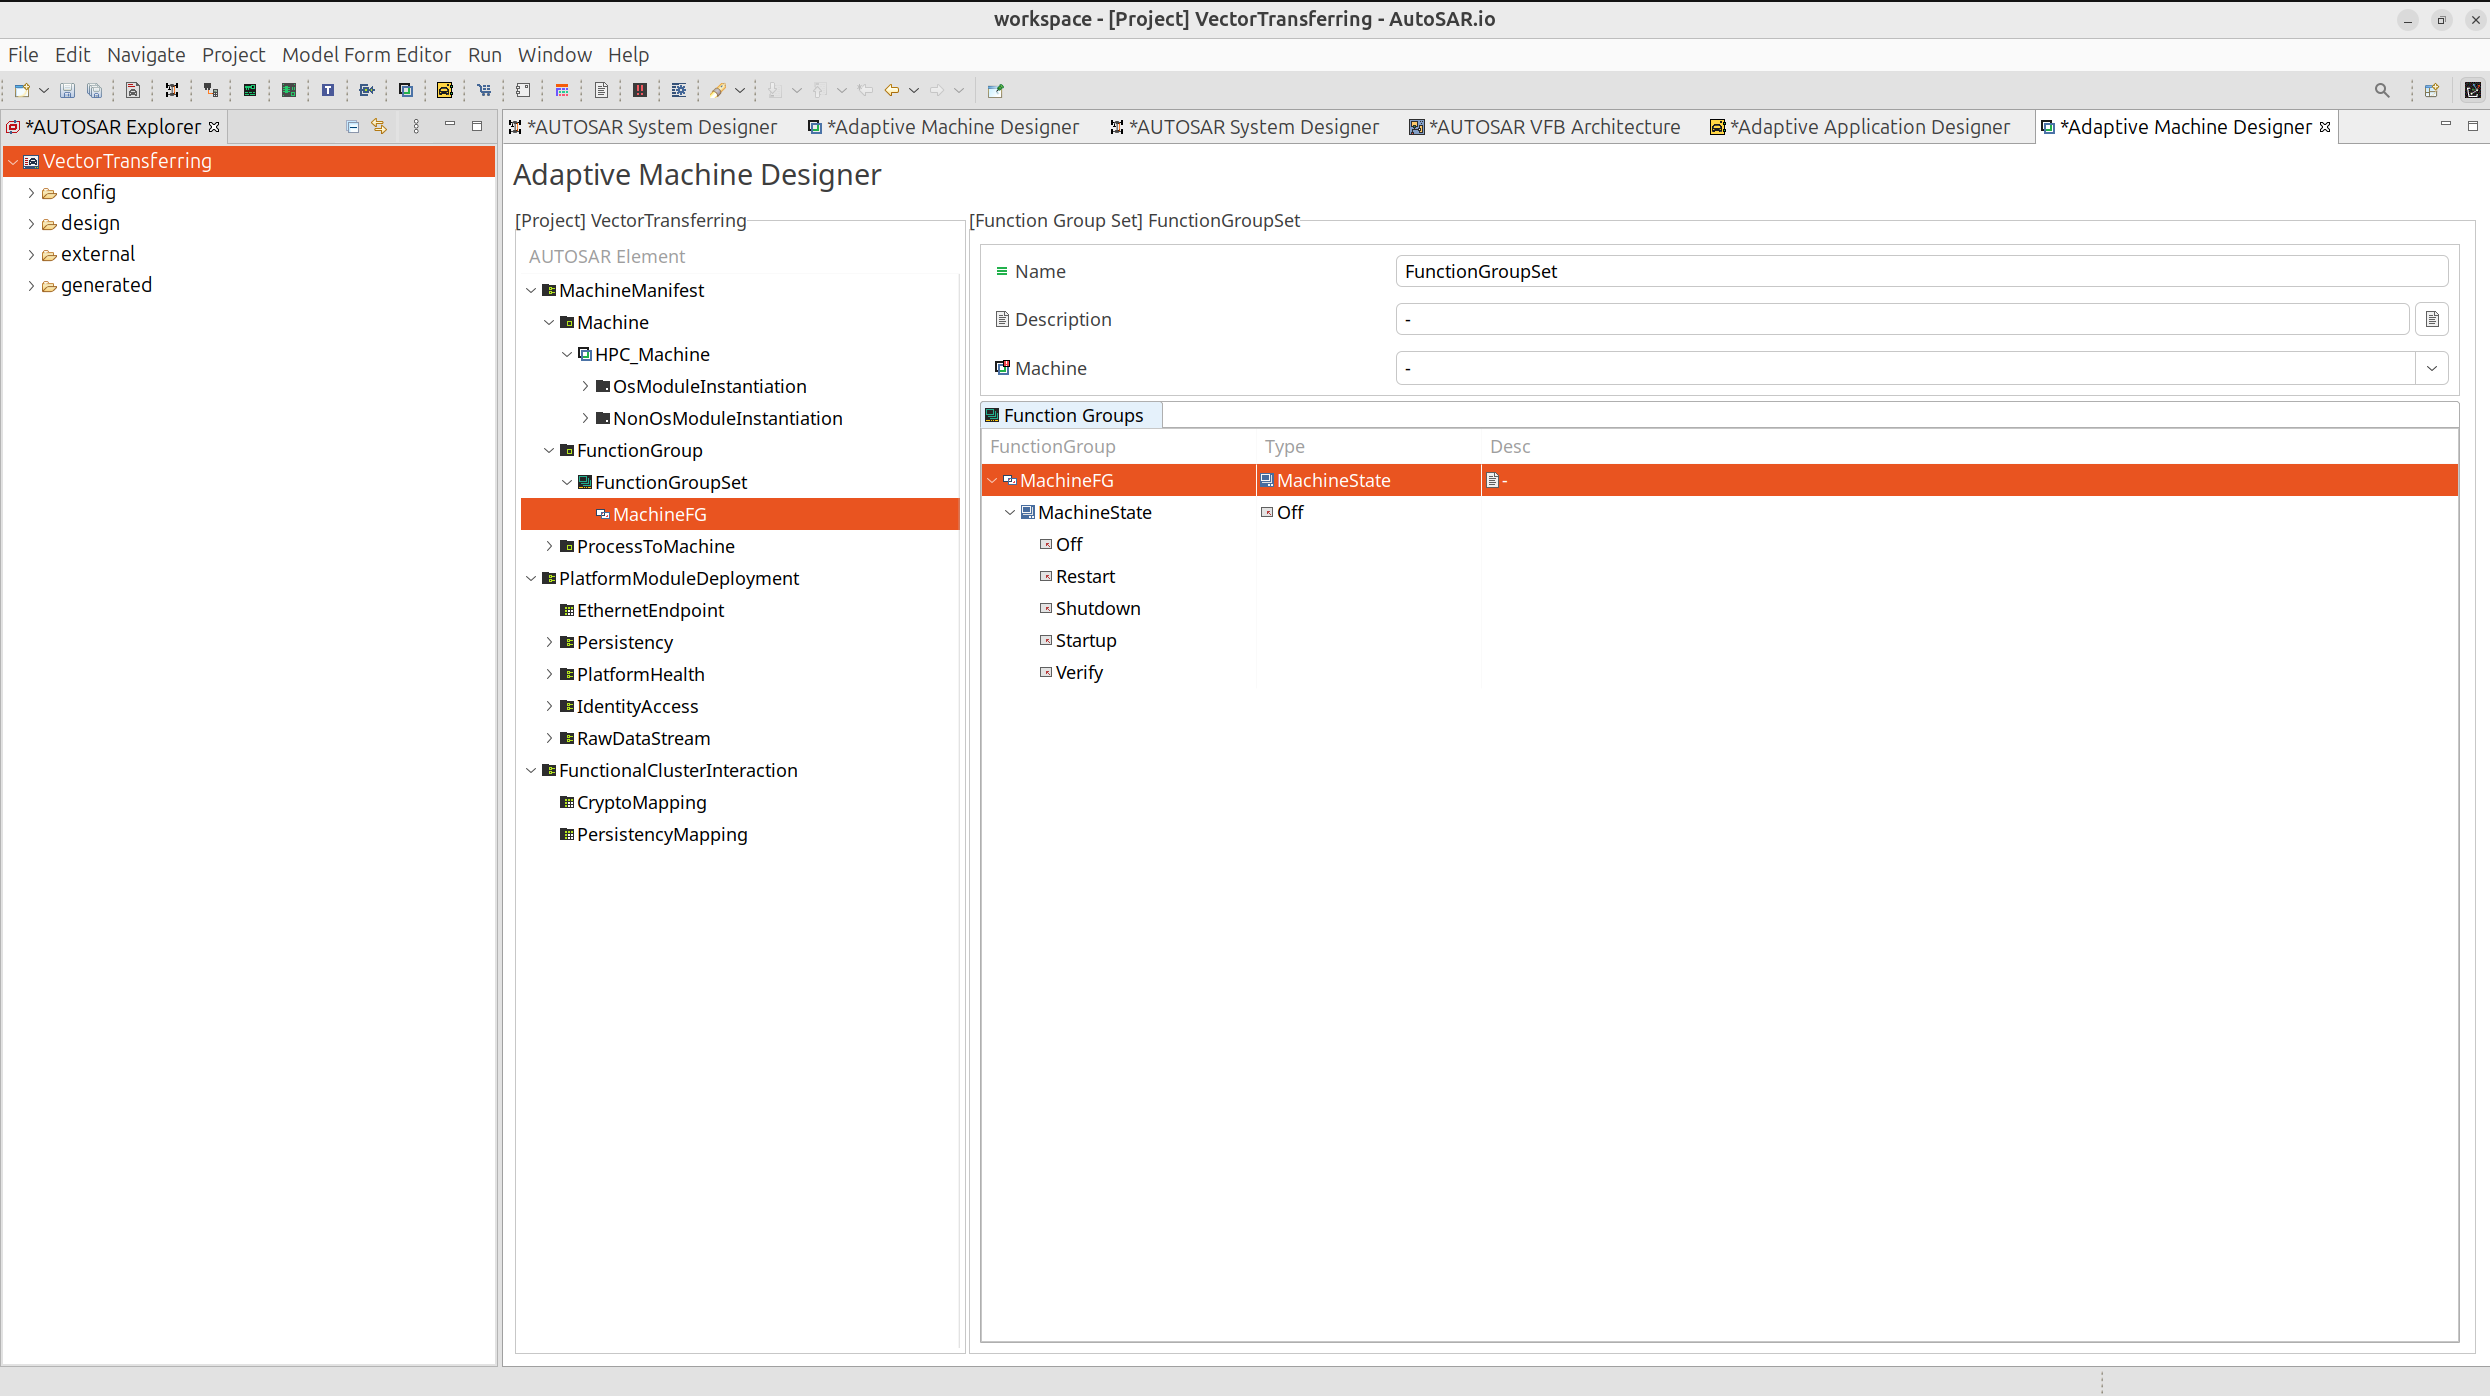
\includegraphics[width=0.75\textwidth]{Images/chap3/image_methodology/machineDesign/configMachineFG.png}
    \vspace{0.5cm}
    \caption{Machine Function Group States Configuration}
    \label{fig:machine_fg_config}
\end{figure}

The figure \ref{fig:machine_fg_config} presents the configuration of the machine function group for the HPC\_Machine in the Adaptive Machine Designer. A function group named MachineFG is defined with the MachineState type, which includes states such as Off, Startup, Verify, Restart, and Shutdown. This configuration governs how the machine progresses through its operational lifecycle, ensuring that platform services and applications are activated and controlled according to well defined system states during runtime execution.

% Final Machine Manifest
\begin{figure}[H]
    \centering
    
\includegraphics[width=0.75\textwidth]{Images/chap3/image_methodology/machineDesign/machineManifest.png}
    \vspace{0.5cm}
    \caption{Machine Manifest for Adaptive AUTOSAR Deployment}
    \label{fig:machine_manifest}
\end{figure}

The figure \ref{fig:machine_manifest} presents the Machine Manifest of the HPC\_Machine as defined in the Adaptive Machine Designer. This manifest consolidates all machine level configurations by referencing the previously defined Machine Design, including the SOME/IP Service Discovery endpoint with the multicast address 224.0.0.1 and port 30490, as well as the Ethernet connector bound to the eth0 interface. In addition, user defined connectors and inter process communication settings are integrated, forming a complete description of the communication capabilities of the target machine.

Furthermore, the manifest specifies essential execution and platform related properties such as trusted platform execution mode, default application timeout, and processor configuration. The processor section defines the available CPU resources and core assignment, while function group and process to machine mappings establish how applications are bound to machine states at runtime. By combining communication, execution, and lifecycle information into a single artifact, the Machine Manifest serves as the final deployment blueprint for Adaptive AUTOSAR applications.

% Configure Operating System platform module
\begin{figure}[H]
    \centering
    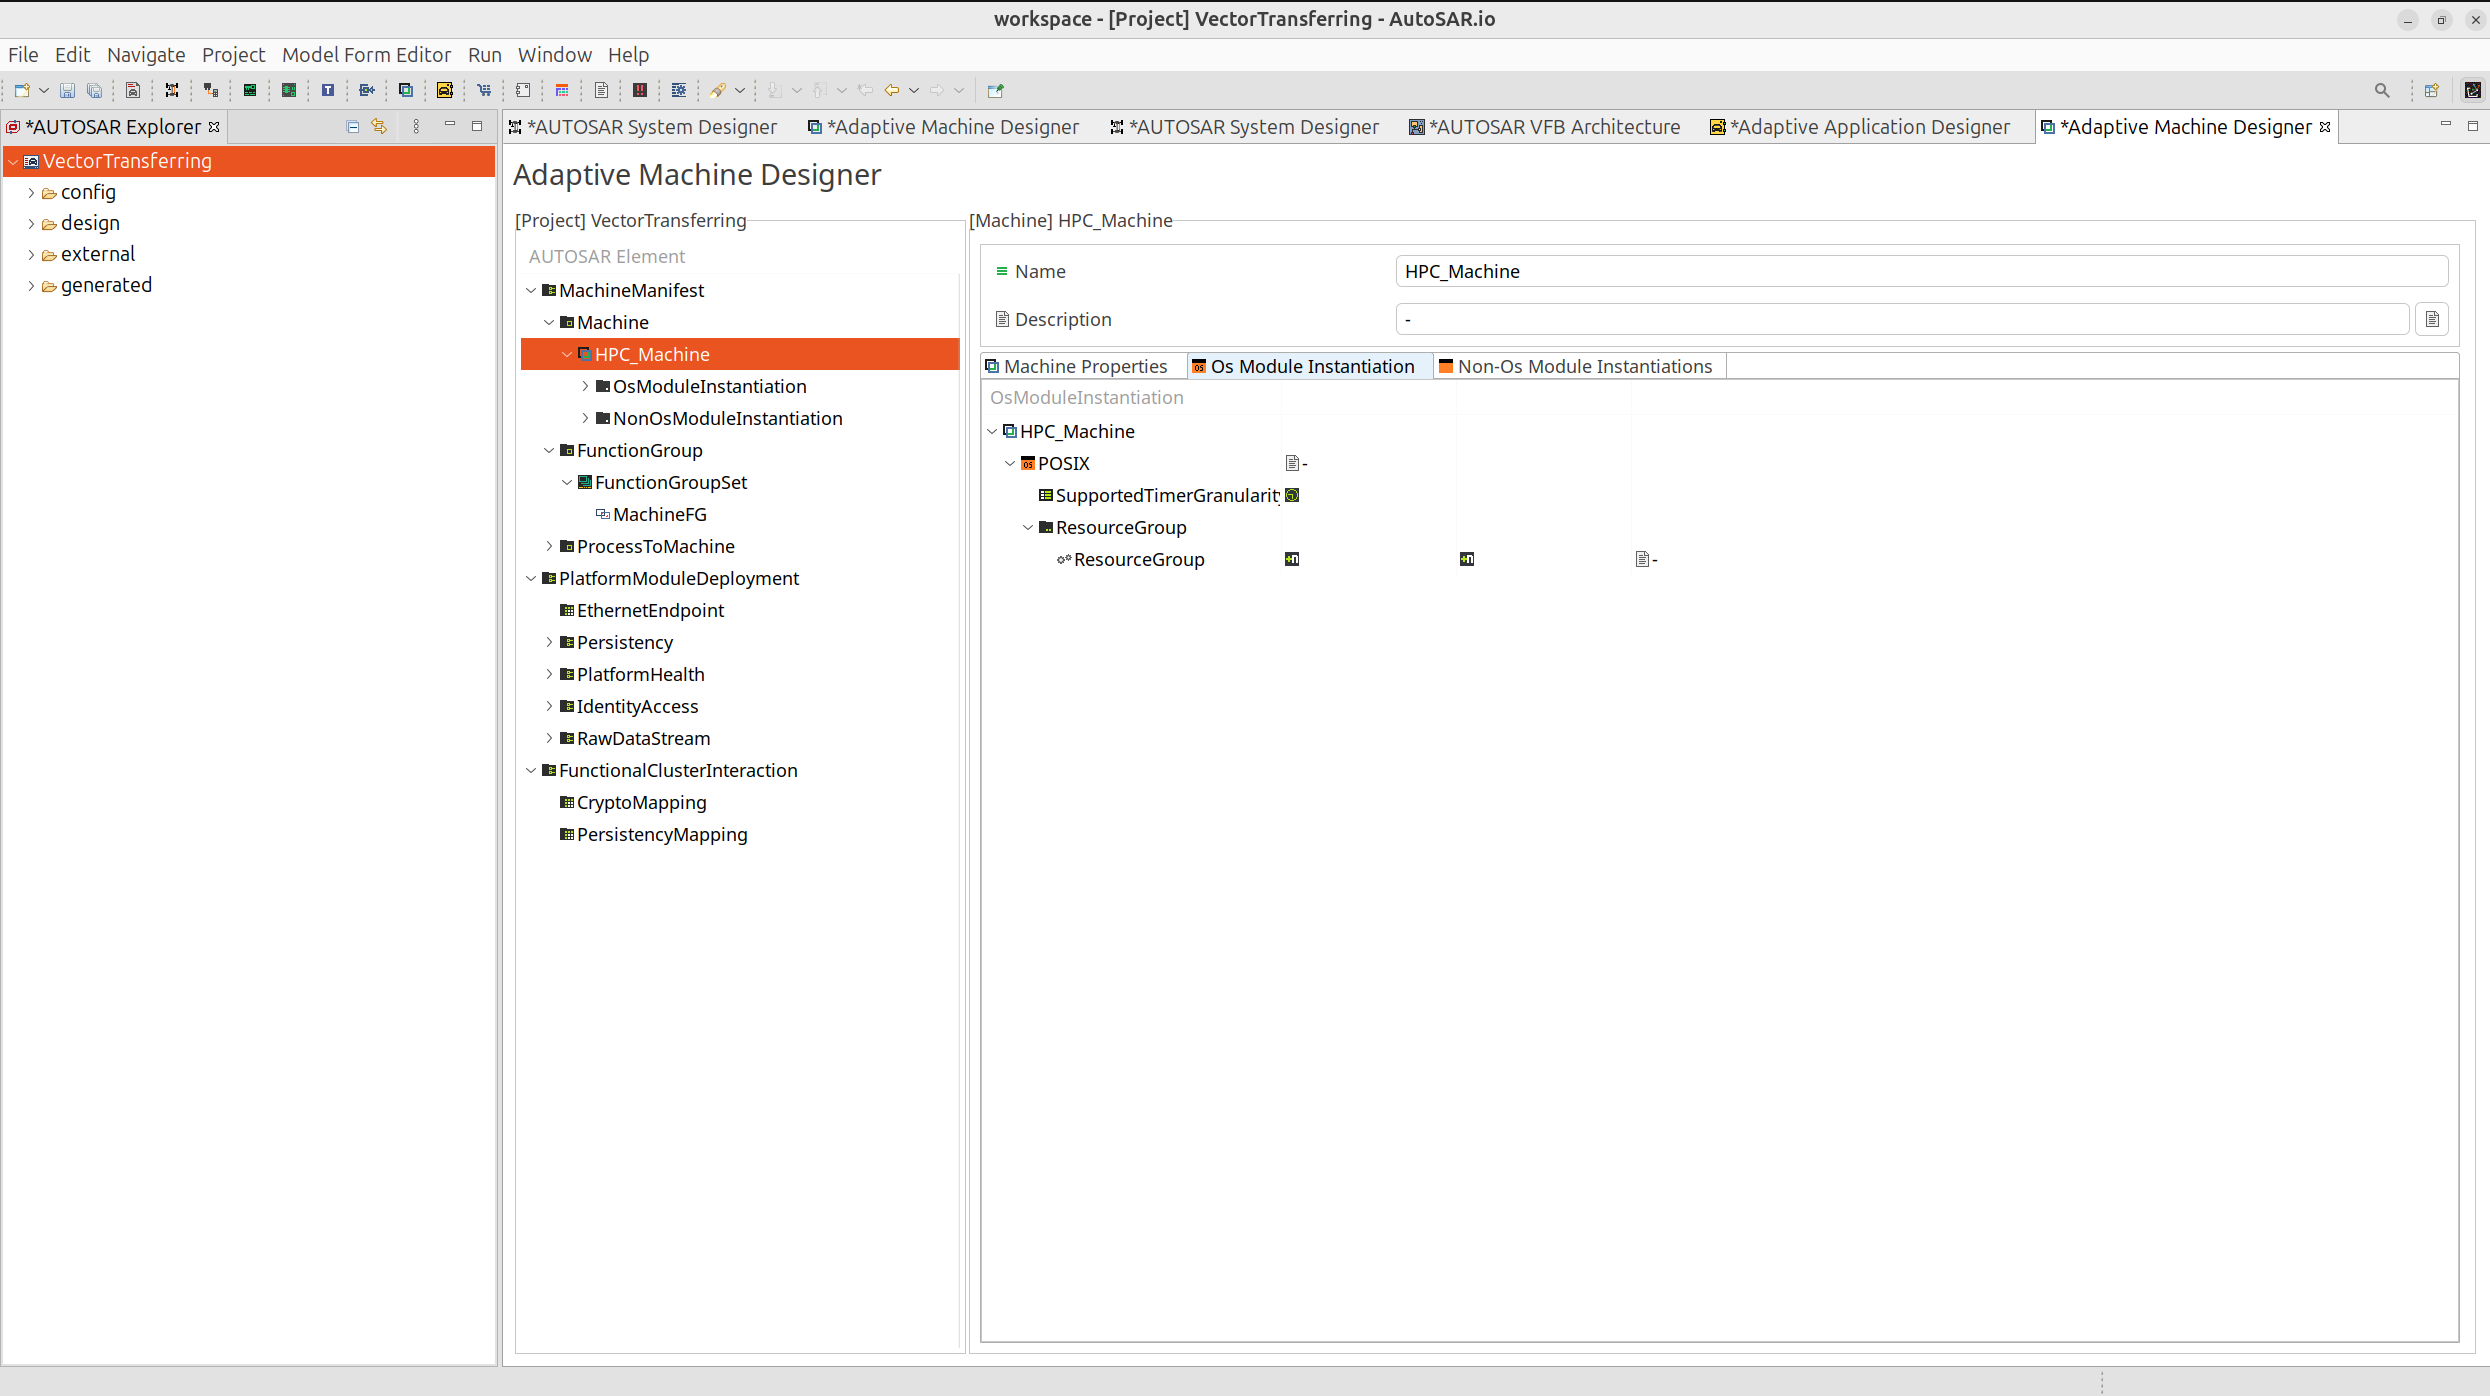
\includegraphics[width=0.75\textwidth]{Images/chap3/image_methodology/machineDesign/configOSModule.png}
    \vspace{0.5cm}
    \caption{Operating System Platform Module Configuration}
    \label{fig:machine_os_module}
\end{figure}

Figure~\ref{fig:machine_os_module} shows the operating system platform module configuration for the target machine named HPC\_Machine in the Adaptive Machine Designer. The POSIX based operating system module is instantiated to define the execution environment for Adaptive AUTOSAR applications, including supported timer granularity and resource group settings. This configuration establishes the fundamental runtime services required for process scheduling and resource management on the target machine.

% Configure non-OS platform modules
\begin{figure}[H]
    \centering
    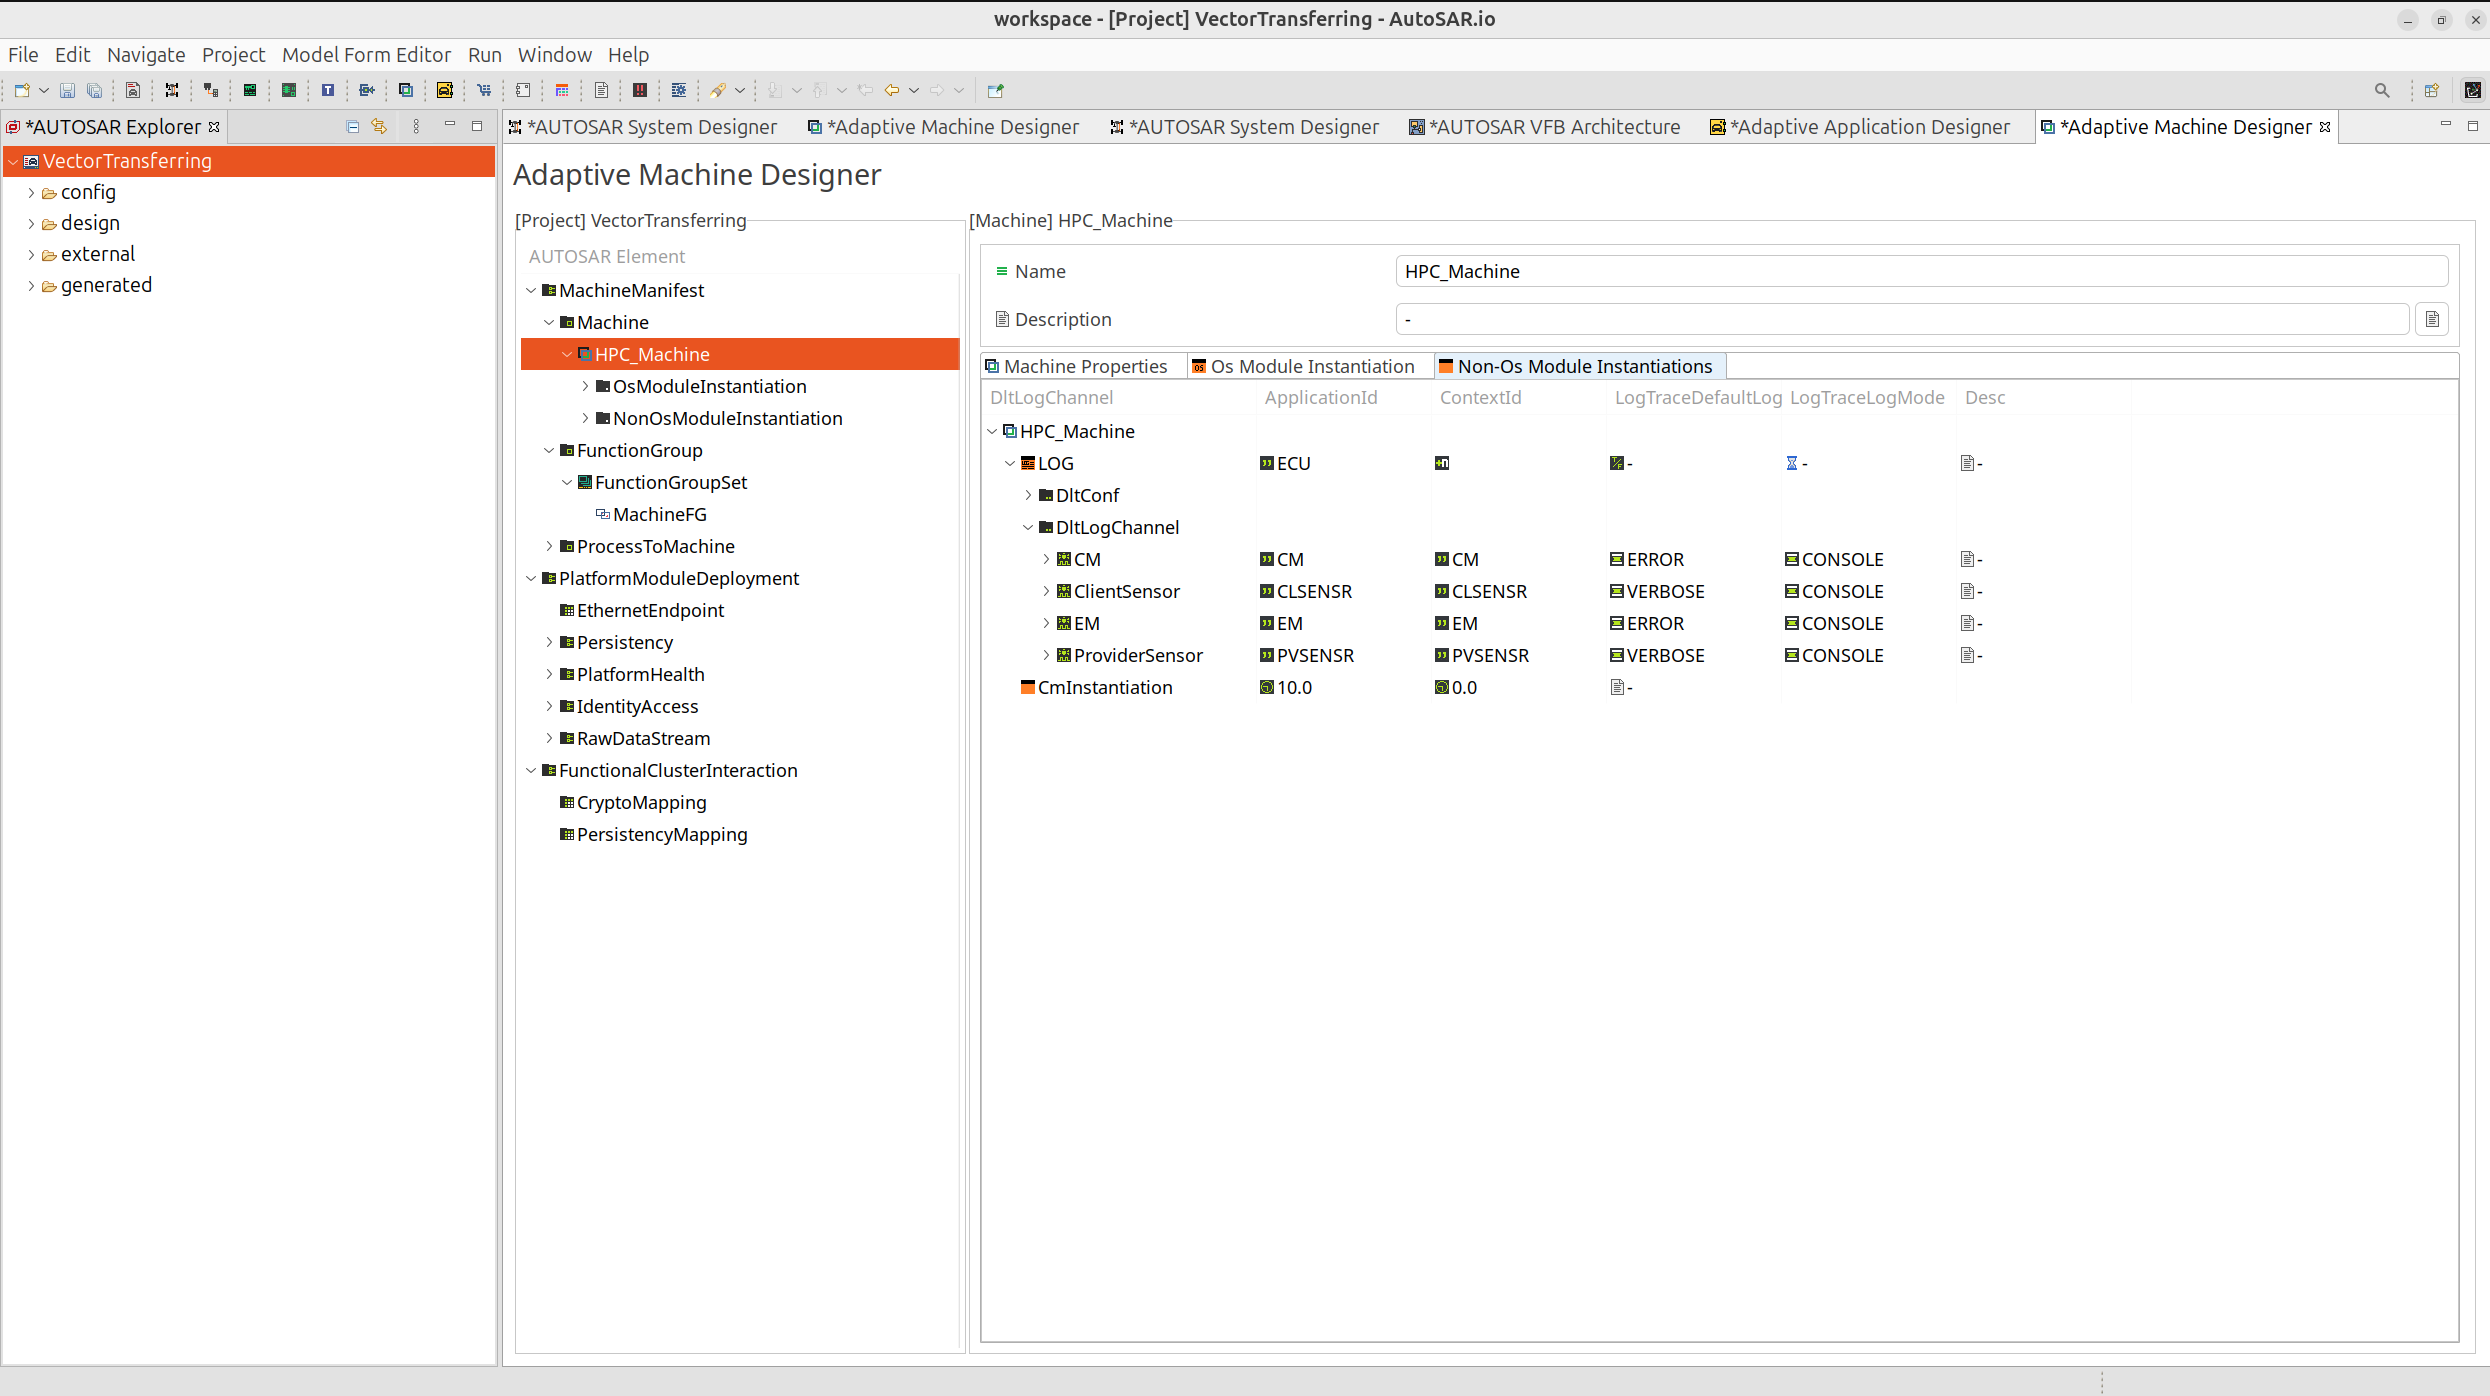
\includegraphics[width=0.75\textwidth]{Images/chap3/image_methodology/machineDesign/configNonOS.png}
    \vspace{0.5cm}
    \caption{Configuration of Non-OS Platform Modules}
    \label{fig:machine_non_os_module}
\end{figure}

Figure~\ref{fig:machine_non_os_module} presents the configuration of Diagnostic Log and Trace for the HPC\_Machine in the Adaptive Machine Designer. Several log channels are defined for different software entities, including ECU, ClientSensor, EM, and ProviderSensor, each mapped to a distinct ApplicationId and ContextId. Log levels such as ERROR and VERBOSE are specified, and the output is directed to the console, allowing developers to monitor application execution and diagnose runtime behavior.

In addition, the configuration highlights the role of CMInstantiation, which represents the Communication Management daemon responsible for inter process communication on the Adaptive Platform. This daemon enables different processes to exchange messages and supports the transport of diagnostic data between applications and platform services. By instantiating the communication manager at the machine level, the system ensures that logging, tracing, and service communication operate coherently across all running processes.

\subsubsection{Service Interface Design and Mapping}

% Define data types for service interfaces
\begin{figure}[H]
    \centering
    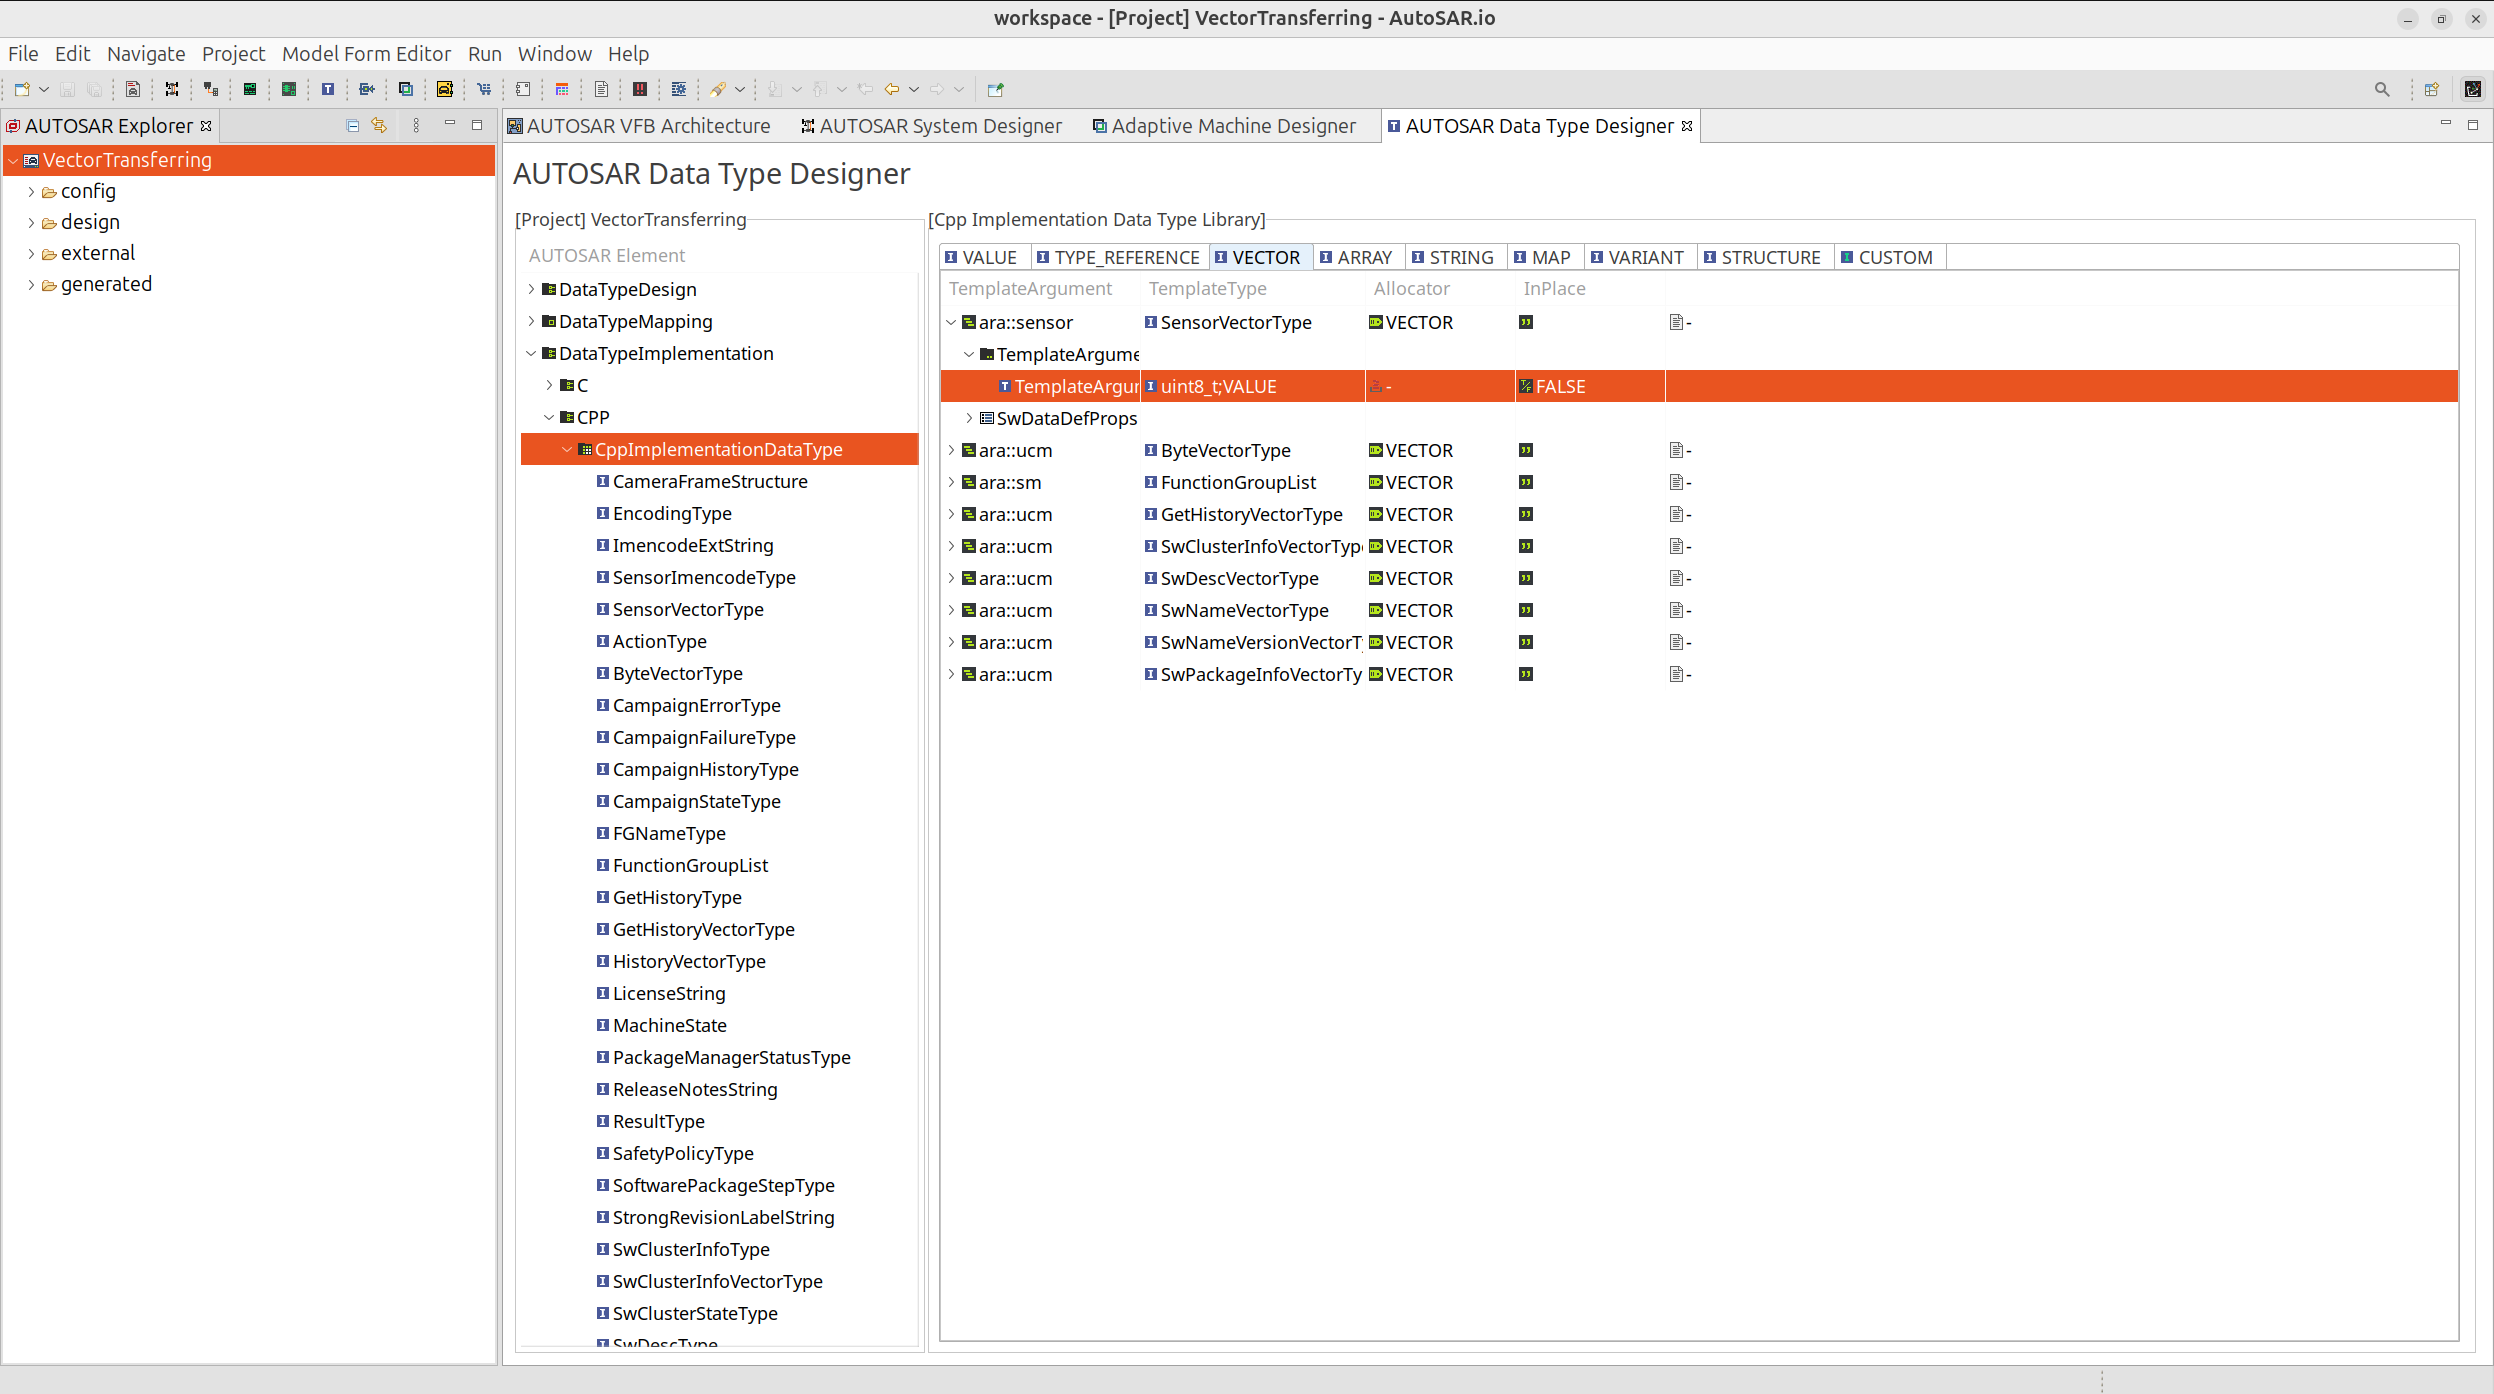
\includegraphics[width=0.75\textwidth]{Images/chap3/image_methodology/serviceInterfaceDesign/dataType.png}
    \vspace{0.5cm}
    \caption{Definition of Data Types for Service Interfaces}
    \label{fig:service_datatype}
\end{figure}

The figure~\ref{fig:service_datatype} shows the specification of C++ data types used to support service interfaces in the Adaptive AUTOSAR environment. Several vector based types are defined using template arguments, where primitive elements such as \texttt{uint8\_t} are combined to represent structured service data. These type definitions provide a clear and reusable foundation for data exchange between service providers and consumers, ensuring consistency and type safety during service oriented communication.

% Define service interface
\begin{figure}[H]
    \centering
    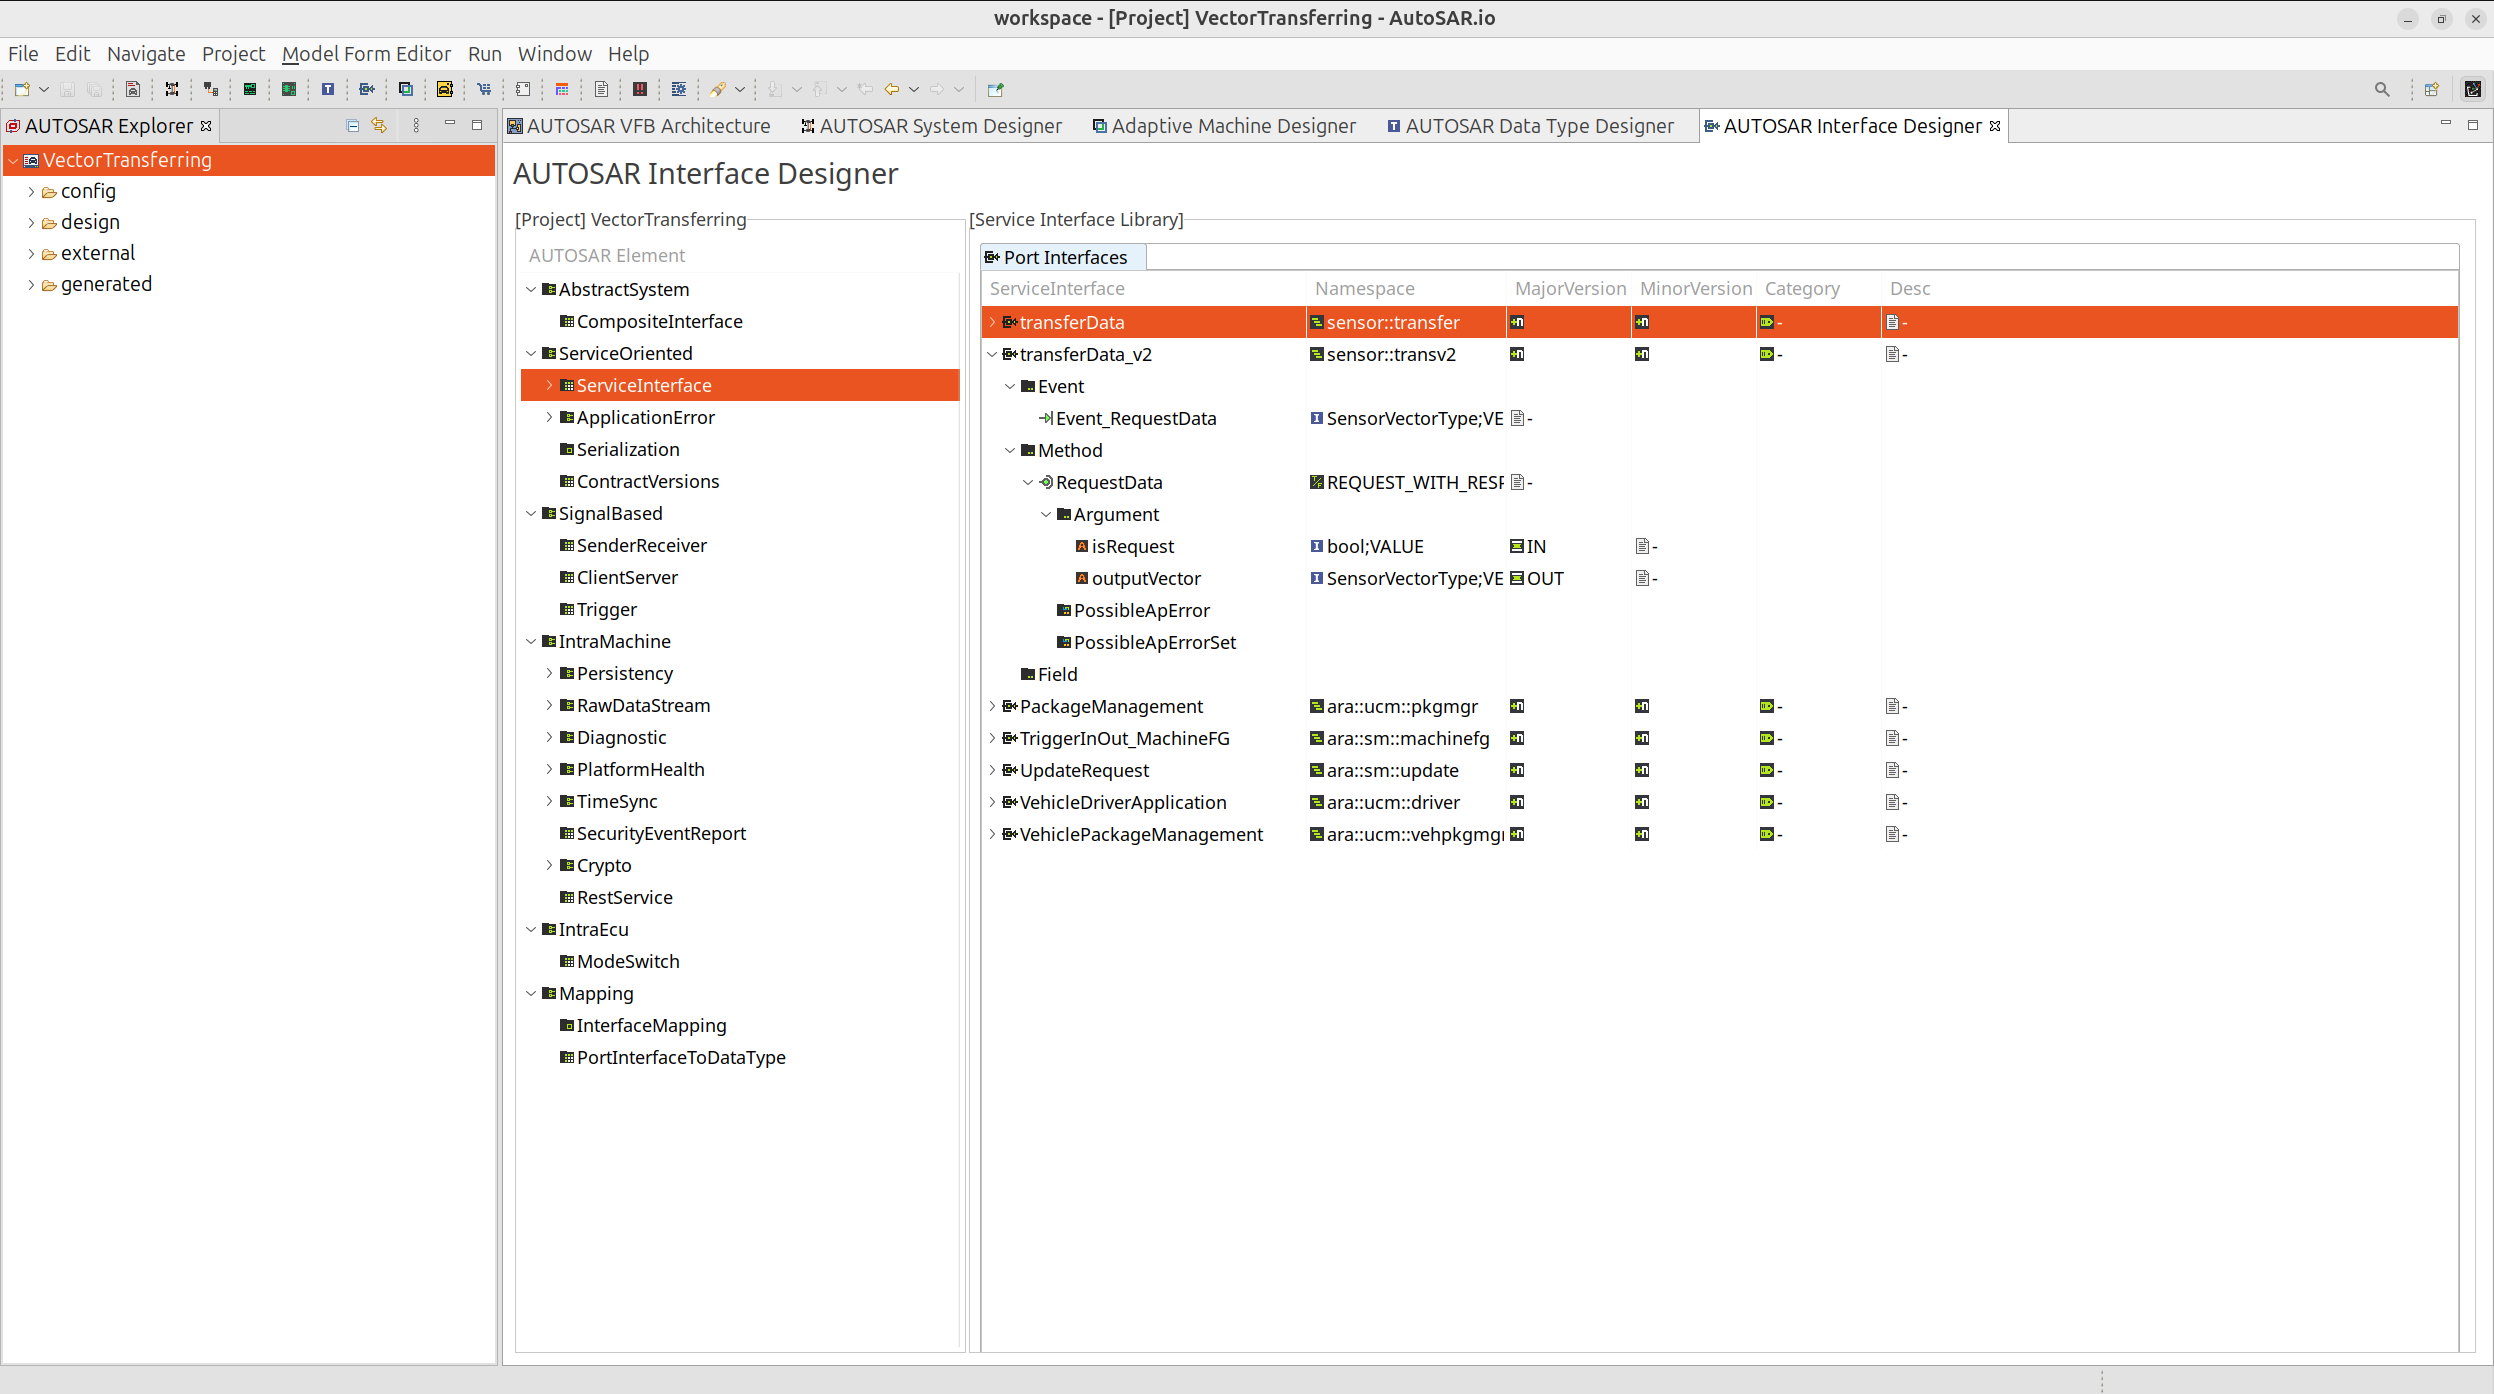
\includegraphics[width=0.75\textwidth]{Images/chap3/image_methodology/serviceInterfaceDesign/defineServiceInterface.png}
    \vspace{0.5cm}
    \caption{Service Interface Definition in Adaptive AUTOSAR}
    \label{fig:service_interface_definition}
\end{figure}

Figure~\ref{fig:service_interface_definition} illustrates the definition of a service oriented interface in the AUTOSAR Interface Designer. The service interface named \texttt{transferData\_v2} is specified within the \texttt{sensor::transv2} namespace and versioned to support interface evolution. It exposes both an event and a method, where the event enables asynchronous notification of data availability, while the method defines a request response interaction pattern for controlled data transmission between applications.

In addition, the interface description includes detailed method arguments and data flow directions. The \texttt{RequestData} method accepts an input parameter that influences the request behavior and produces an output vector based on the previously defined sensor data type. The event is associated with the same data representation (\texttt{Event\_RequestData}), allowing consumers to receive updates without explicitly issuing a request. Possible application errors are also declared to handle exceptional conditions during execution. As shown in Figure~\ref{fig:service_interface_definition}, this interface design supports both reactive and on demand communication between service providers and consumers in the Adaptive AUTOSAR system.


% Service deployment configuration
\begin{figure}[H]
    \centering
    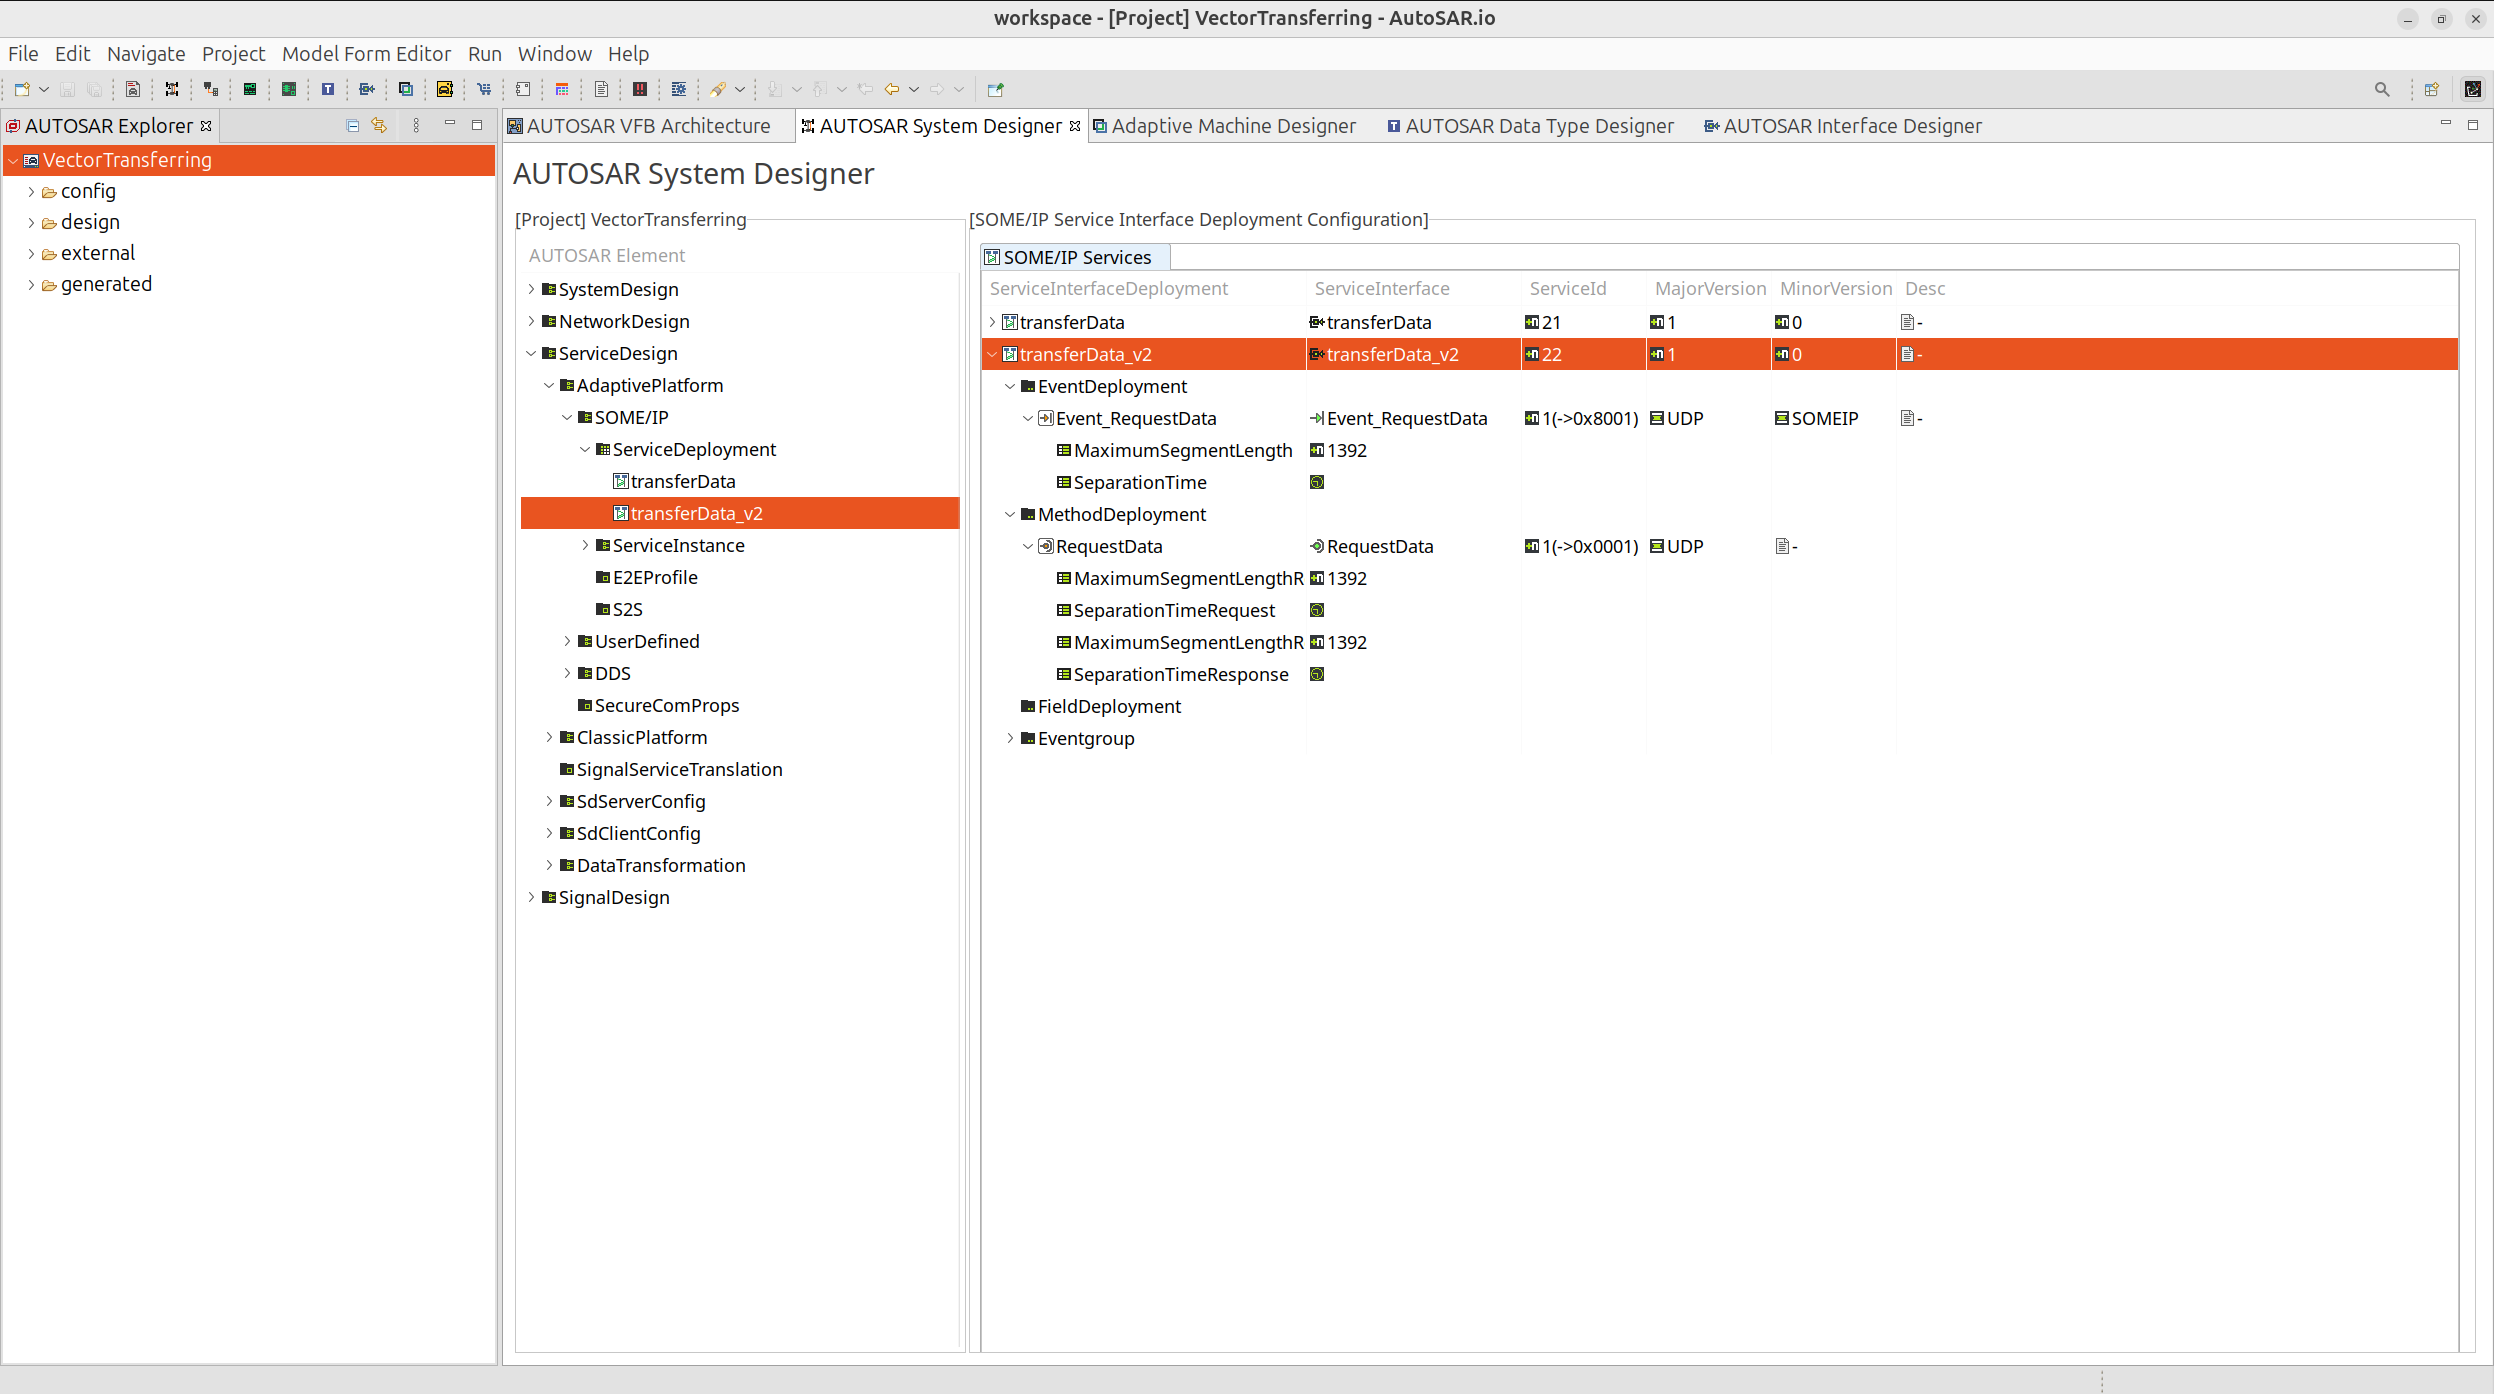
\includegraphics[width=0.75\textwidth]{Images/chap3/image_methodology/serviceInterfaceDesign/serviceDeployment.png}
    \vspace{0.5cm}
    \caption{Service Deployment Configuration}
    \label{fig:service_deployment}
\end{figure}

Figure~\ref{fig:service_deployment} illustrates the SOME/IP service deployment configuration for the \texttt{transferData\_v2} interface within the AUTOSAR System Designer. In this project, the service is explicitly deployed over SOME/IP with transport protocol (SOME/IP-TP) to support the transmission of large data payloads, such as image frames, between the ProviderSensor and ClientSensor applications.

The service is assigned a unique service identifier and version number and includes both event-based and method-based communication. The event \texttt{Event\_RequestData} is configured to use UDP transport together with a specified \texttt{MaximumSegmentLength}. This parameter plays a critical role in enabling SOME/IP-TP, as it informs the Adaptive AUTOSAR middleware that the transmitted data may exceed the maximum payload size of a single UDP packet and therefore must be segmented and reassembled at the receiver side.

Without configuring the \texttt{MaximumSegmentLength}, the communication would default to standard SOME/IP over UDP, which is suitable only for small messages and is not appropriate for transmitting image data. By explicitly defining this parameter, the deployment ensures that image payloads generated by the ProviderSensor are correctly fragmented, transmitted, and reassembled by the ClientSensor.

In addition to the event deployment, the \texttt{RequestData} method deployment specifies request and response timing parameters, supporting controlled client–server interaction when on-demand data transfer is required. Together, these configurations ensure that the \texttt{transferData\_v2} service can be reliably discovered via Service Discovery and can support both event-driven and request-based communication over SOME/IP-TP during runtime execution.


% Service instance provider configuration
\begin{figure}[H]
    \centering
    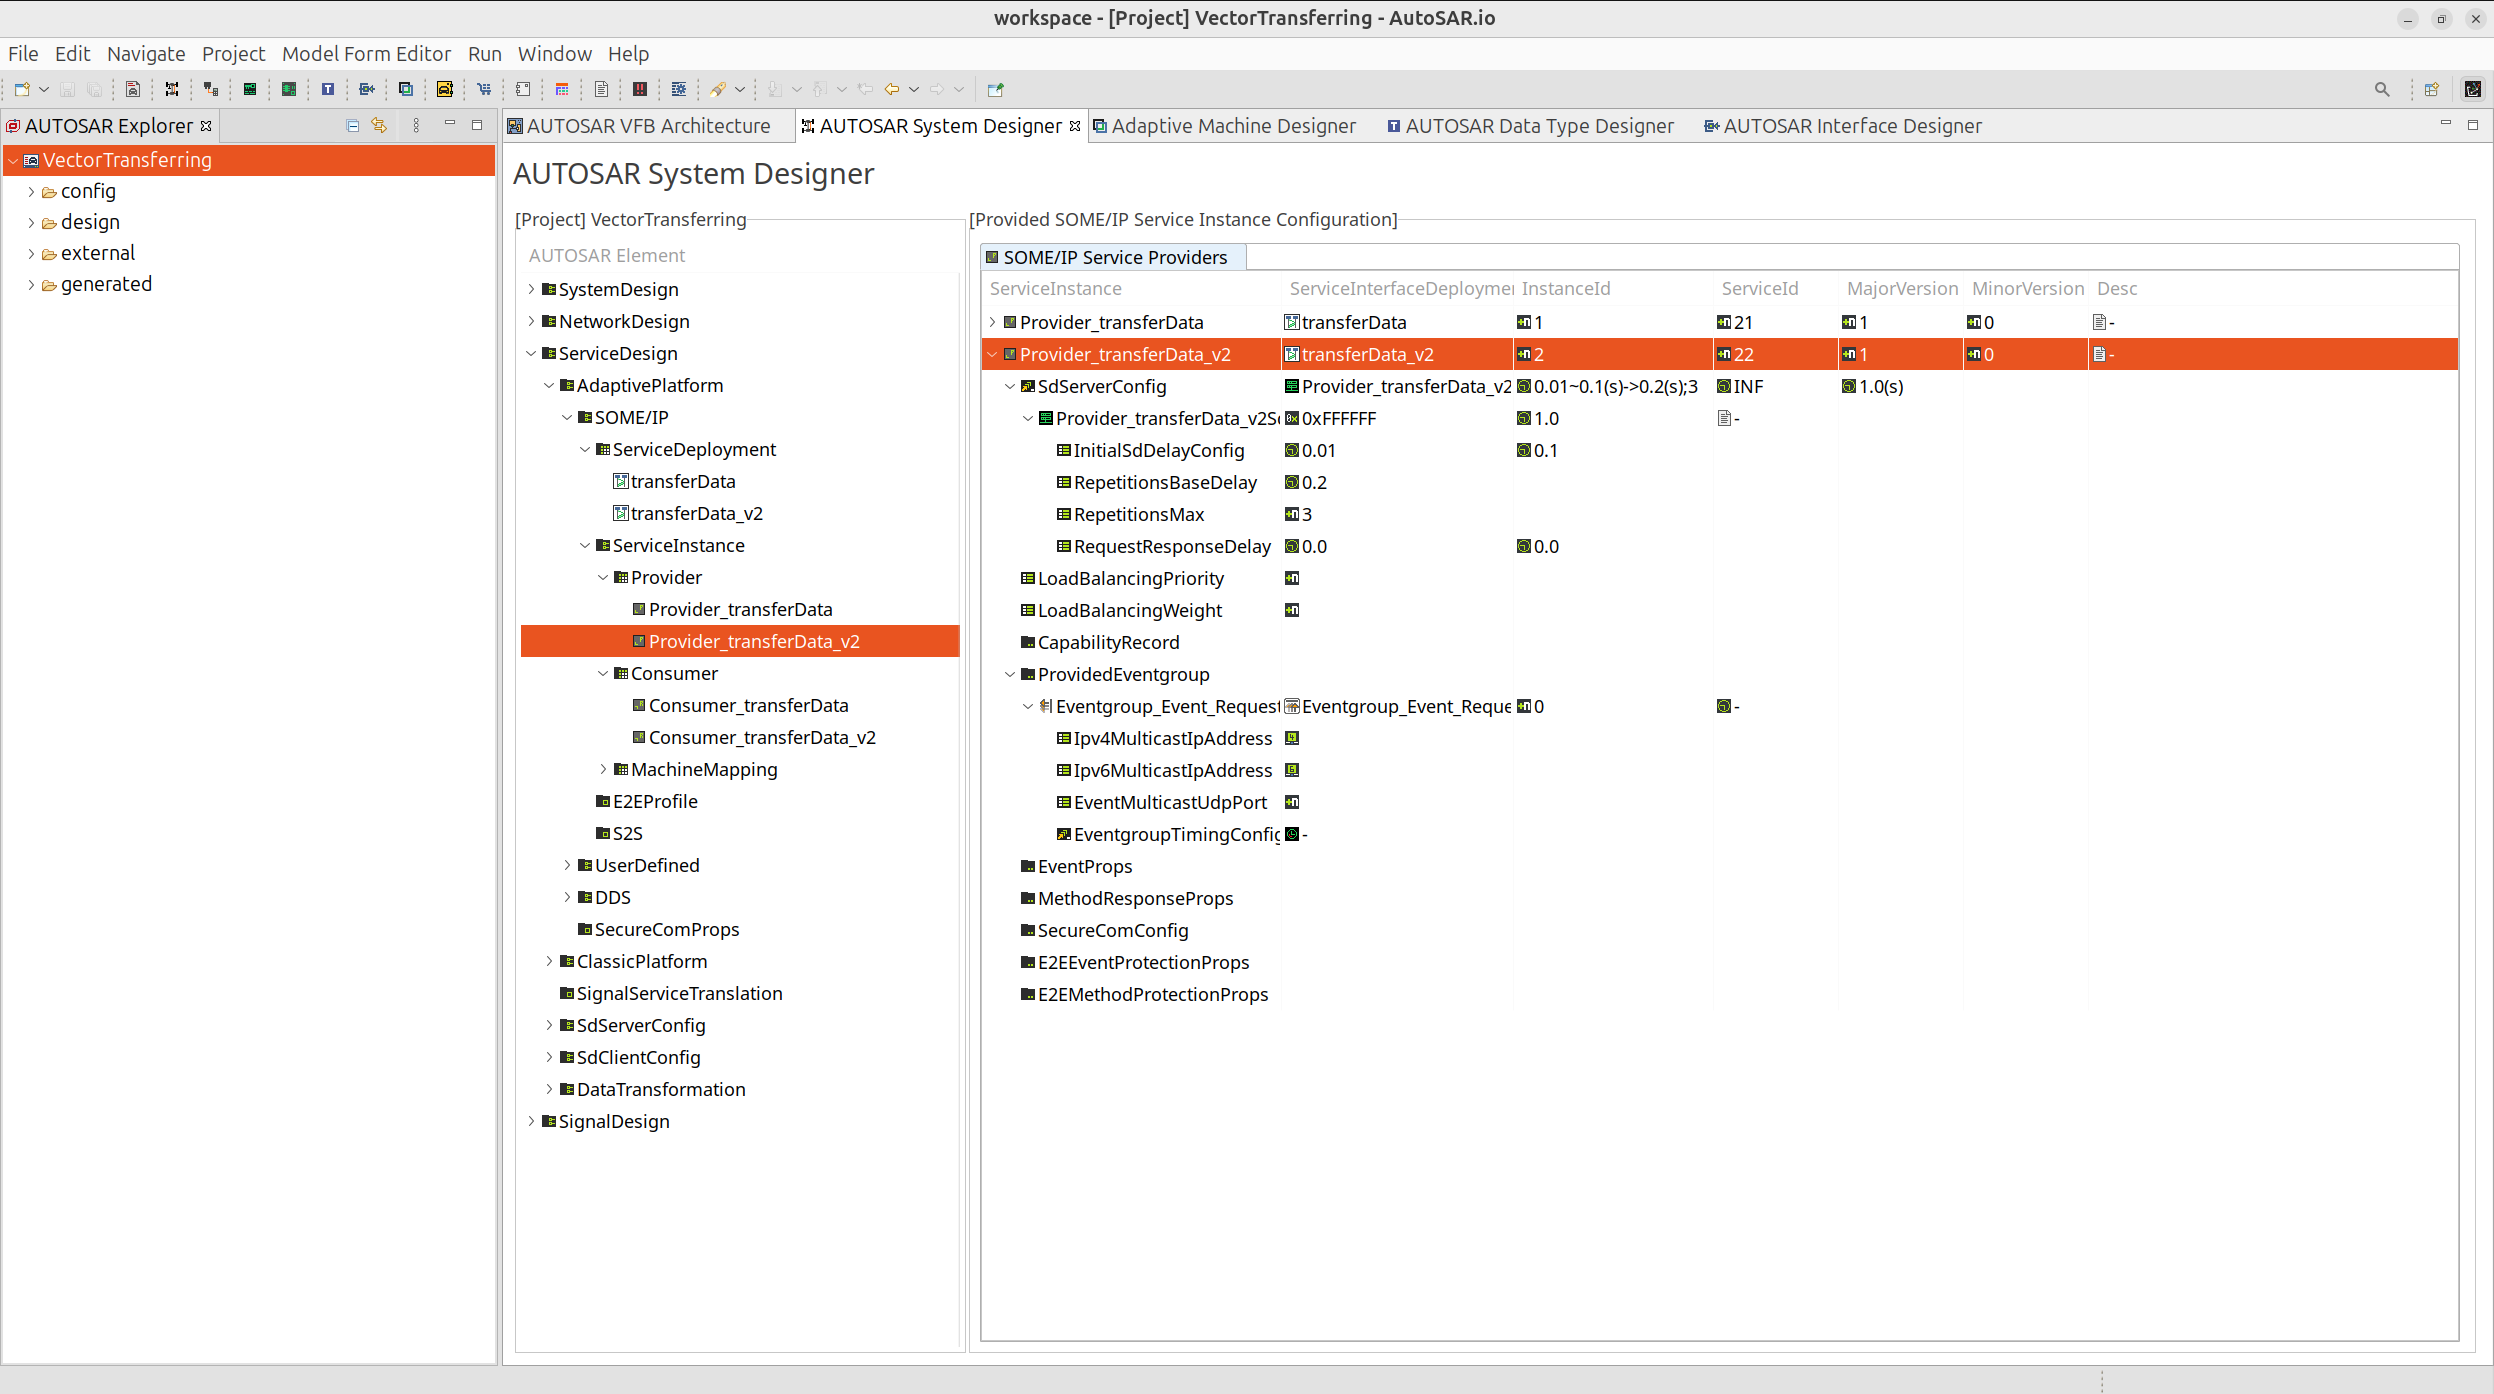
\includegraphics[width=0.75\textwidth]{Images/chap3/image_methodology/serviceInterfaceDesign/serviceInstance_Provider.png}
    \vspace{0.5cm}
    \caption{Service Instance Configuration for Provider}
    \label{fig:service_instance_provider}
\end{figure}

Figure~\ref{fig:service_instance_provider} illustrates the configuration of the SOME/IP service provider for the \texttt{transferData\_v2} interface. The provider instance is bound to a specific service and instance identifier with a defined major and minor version, ensuring compatibility with consuming applications. Server side parameters such as initial service offer delay, repetition base delay, and maximum repetitions are configured to control service availability announcements via Service Discovery. In addition, the provider defines event group settings for data notifications, together with timing and response related properties, which enable reliable dissemination of event based data to subscribed consumers during runtime.

% Service instance consumer configuration
\begin{figure}[H]
    \centering
    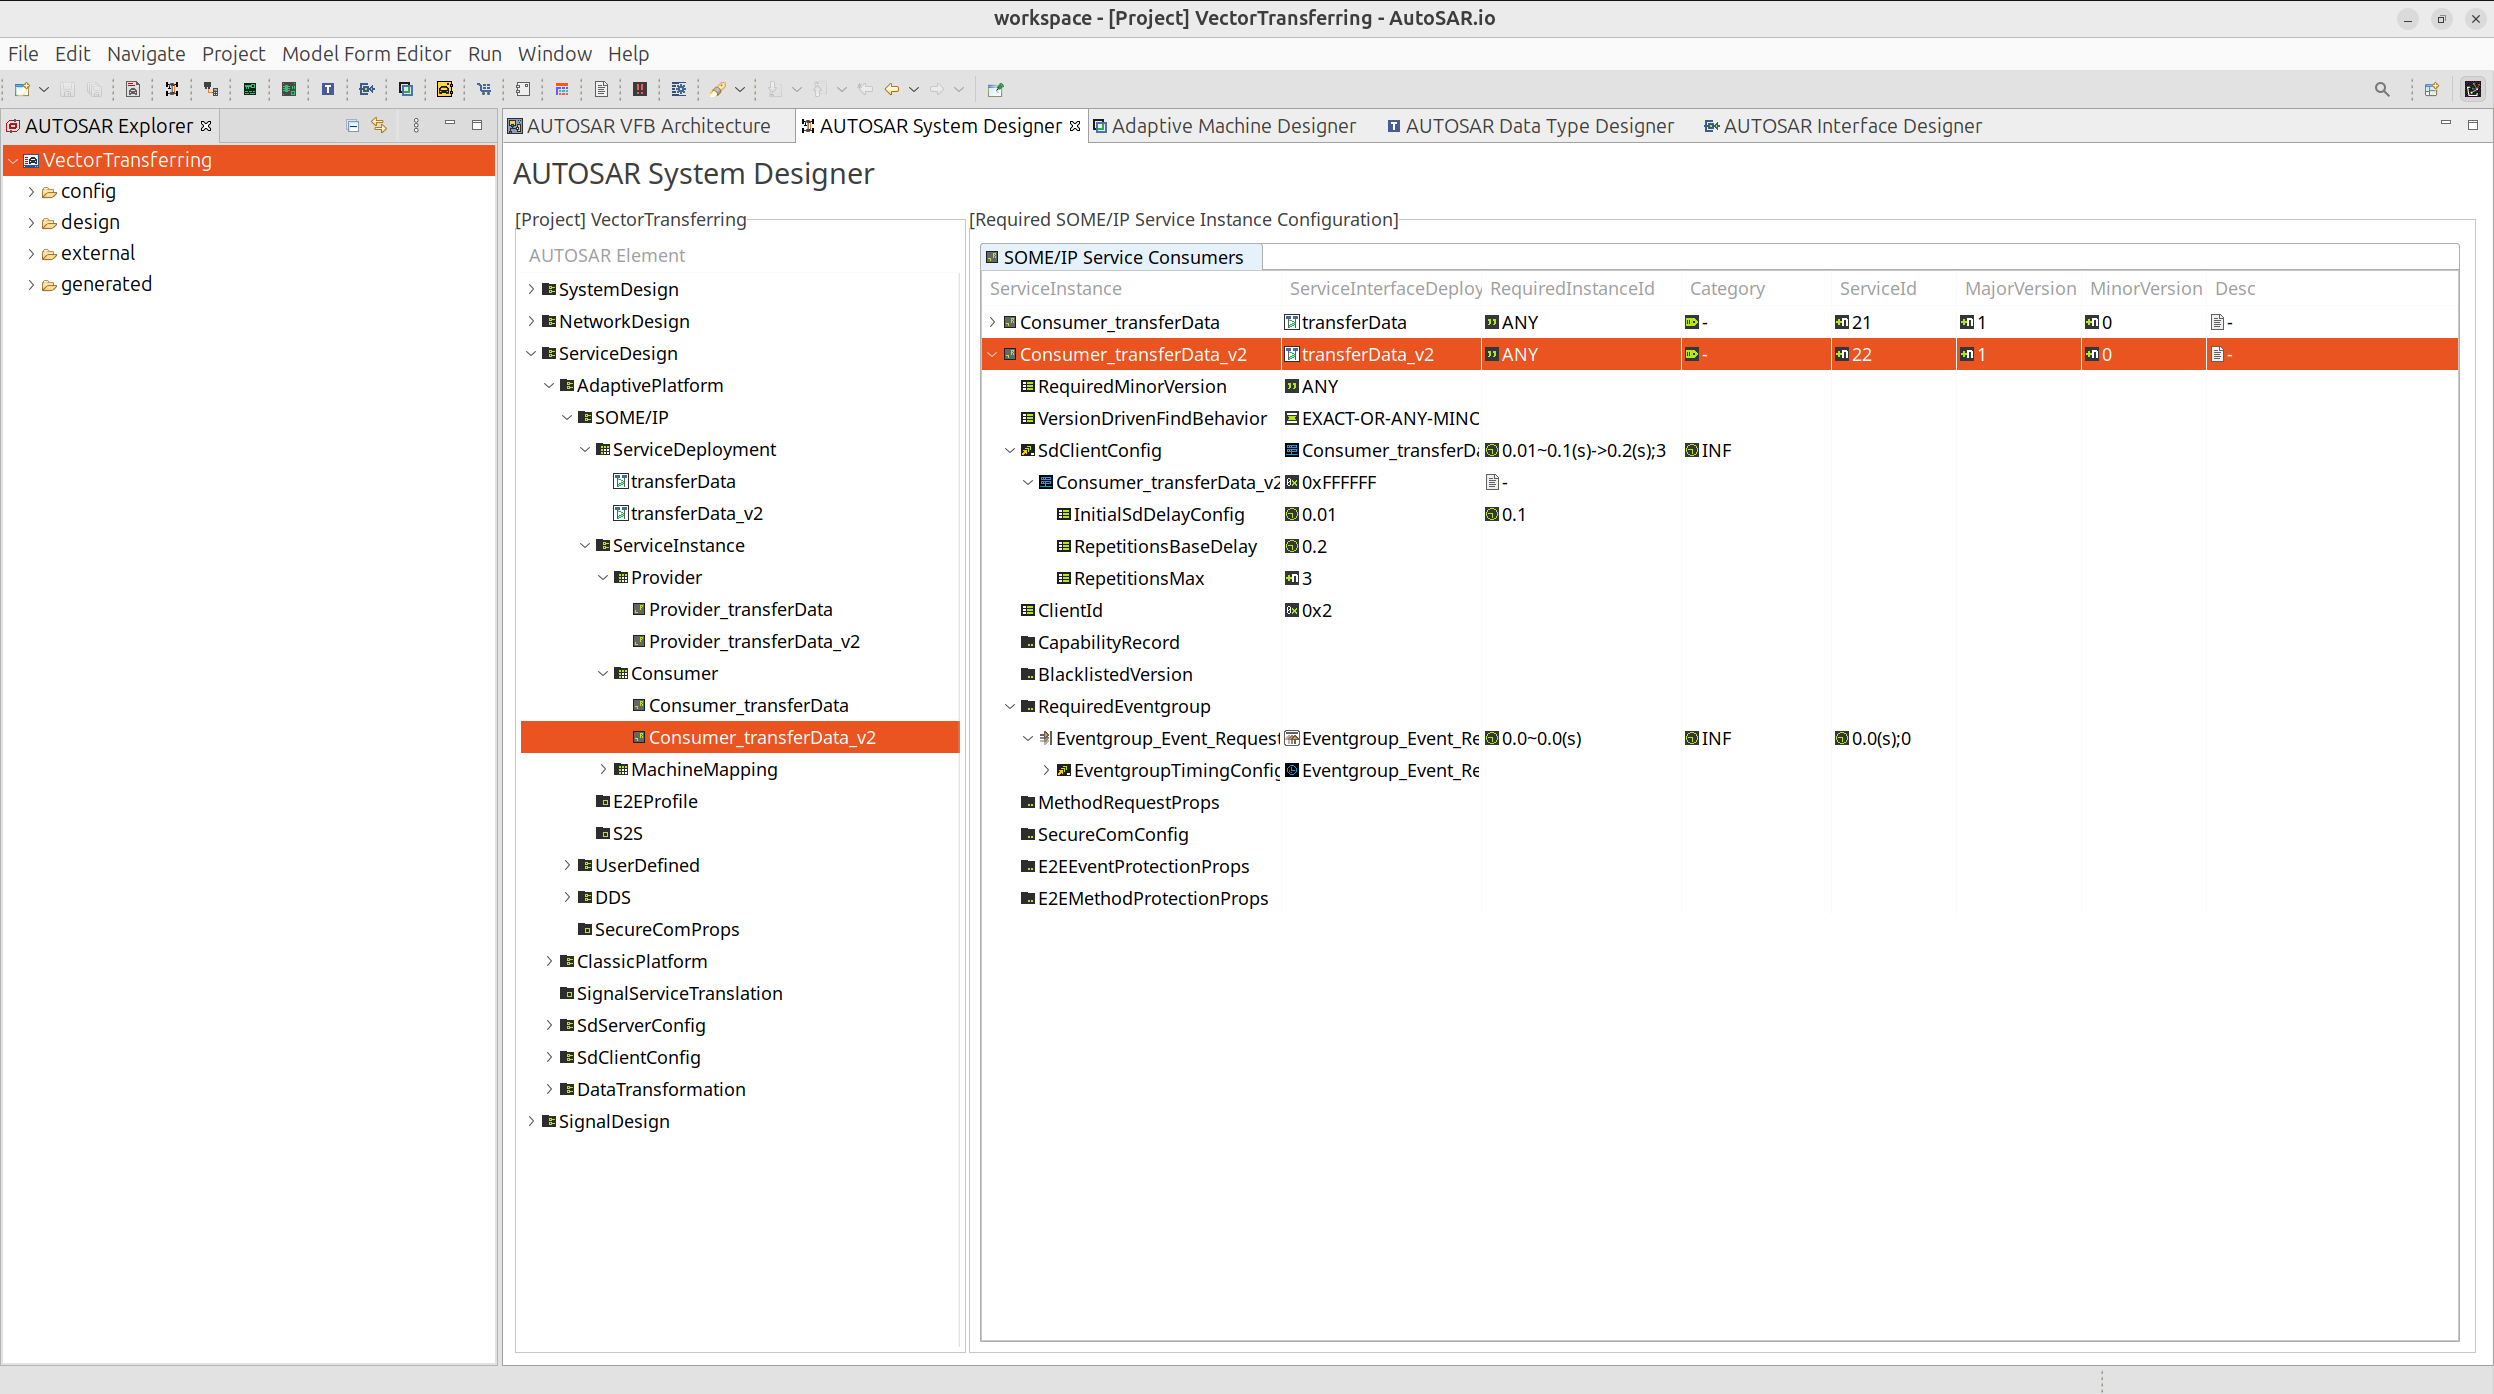
\includegraphics[width=0.75\textwidth]{Images/chap3/image_methodology/serviceInterfaceDesign/serviceInstance_Consumer.png}
    \vspace{0.5cm}
    \caption{Service Instance Configuration for Consumer}
    \label{fig:service_instance_consumer}
\end{figure}

Figure~\ref{fig:service_instance_consumer} presents the configuration of the corresponding SOME/IP service consumer acting as a subscriber to the \texttt{transferData\_v2} service. The consumer specifies flexible version requirements and discovery behavior, allowing it to bind to compatible provider instances at runtime. Client side parameters such as initial request delay, repetition strategy, and event group subscription settings determine how the consumer discovers the service and receives event notifications. Through this configuration, the consumer can dynamically subscribe to published data while maintaining controlled request and subscription behavior within the Adaptive AUTOSAR communication framework.

% Mapping service to machine network endpoint
\begin{figure}[H]
    \centering
    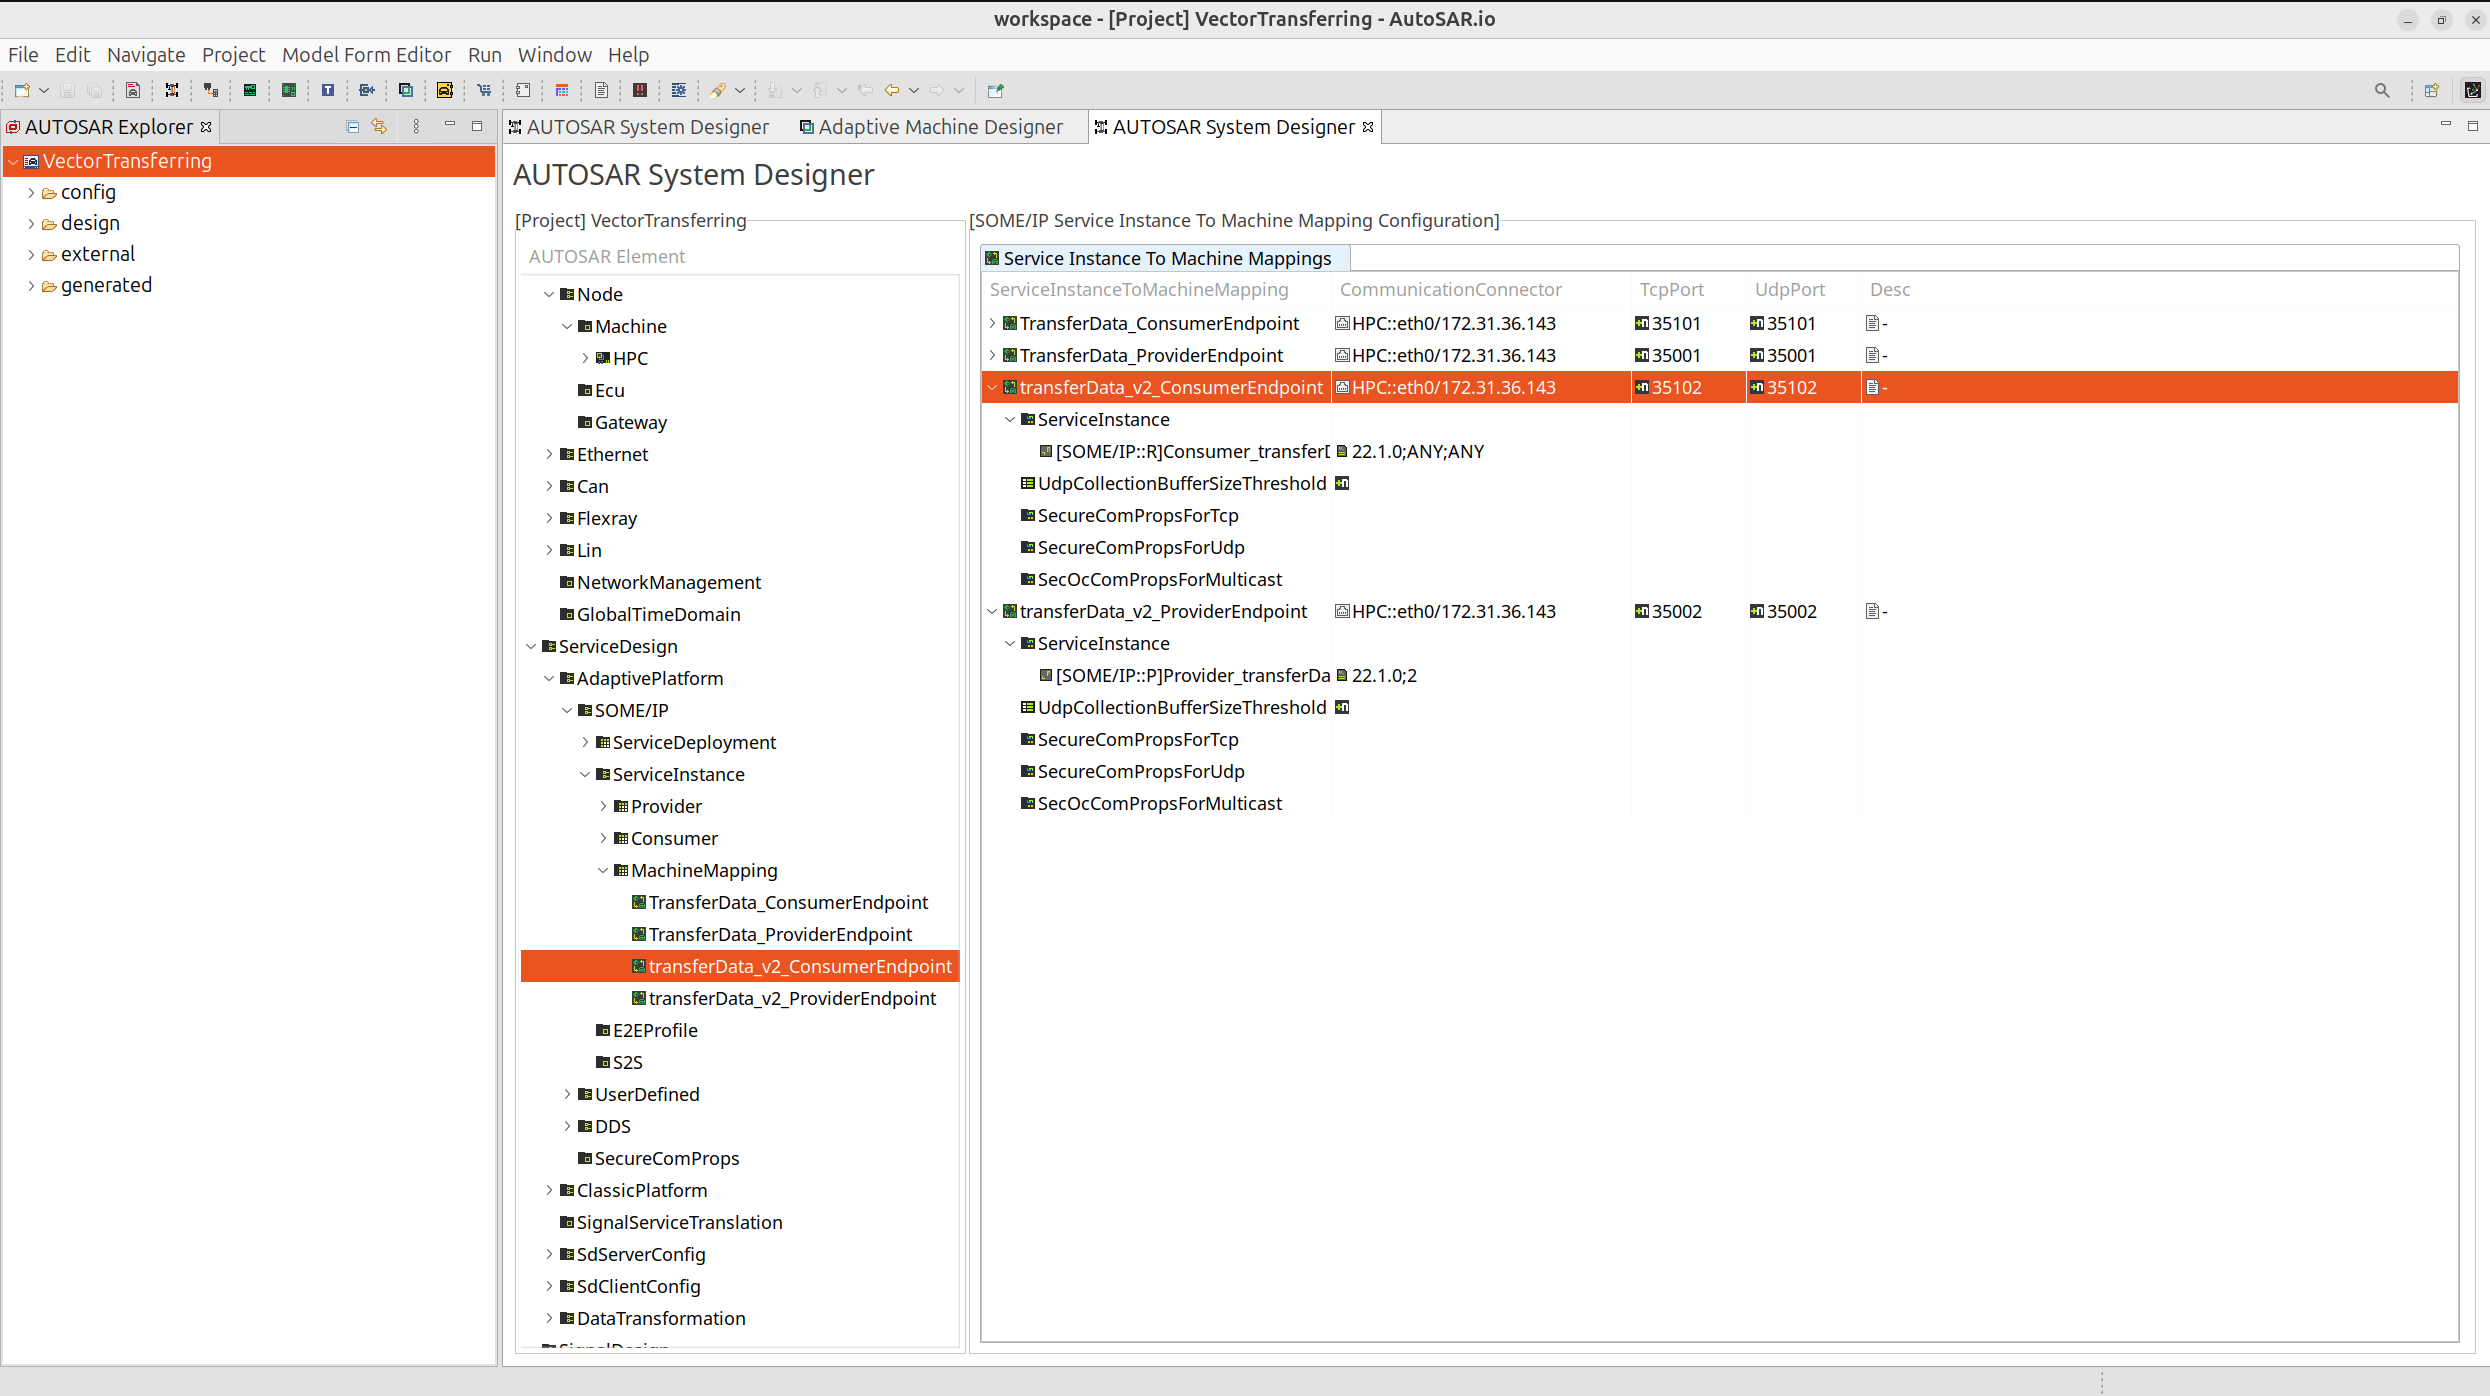
\includegraphics[width=0.75\textwidth]{Images/chap3/image_methodology/serviceInterfaceDesign/serviceMappingMachineEndpoint.png}
    \vspace{0.5cm}
    \caption{Mapping Service Instances to Machine Network Endpoint}
    \label{fig:service_machine_endpoint_mapping}
\end{figure}

Figure~\ref{fig:service_machine_endpoint_mapping} illustrates how the service instances of the \texttt{transferData} and \texttt{transferData\_v2} interfaces are bound to concrete machine network endpoints. Both provider and consumer instances are mapped to the Ethernet communication connector \texttt{HPC:eth0} with the fixed IPv4 address \texttt{172.31.36.143}, ensuring that all service communication is routed through a well defined network interface. Distinct TCP and UDP port numbers are assigned to each service instance, allowing concurrent data exchange while avoiding port conflicts.

This mapping explicitly links abstract service definitions to physical network resources, enabling correct runtime deployment and communication over SOME/IP. By defining separate endpoints for provider and consumer roles, the configuration supports clear role separation and reliable message routing between applications deployed on the same machine or across different nodes in the Adaptive AUTOSAR system.

\begin{figure}[H]
    \centering
    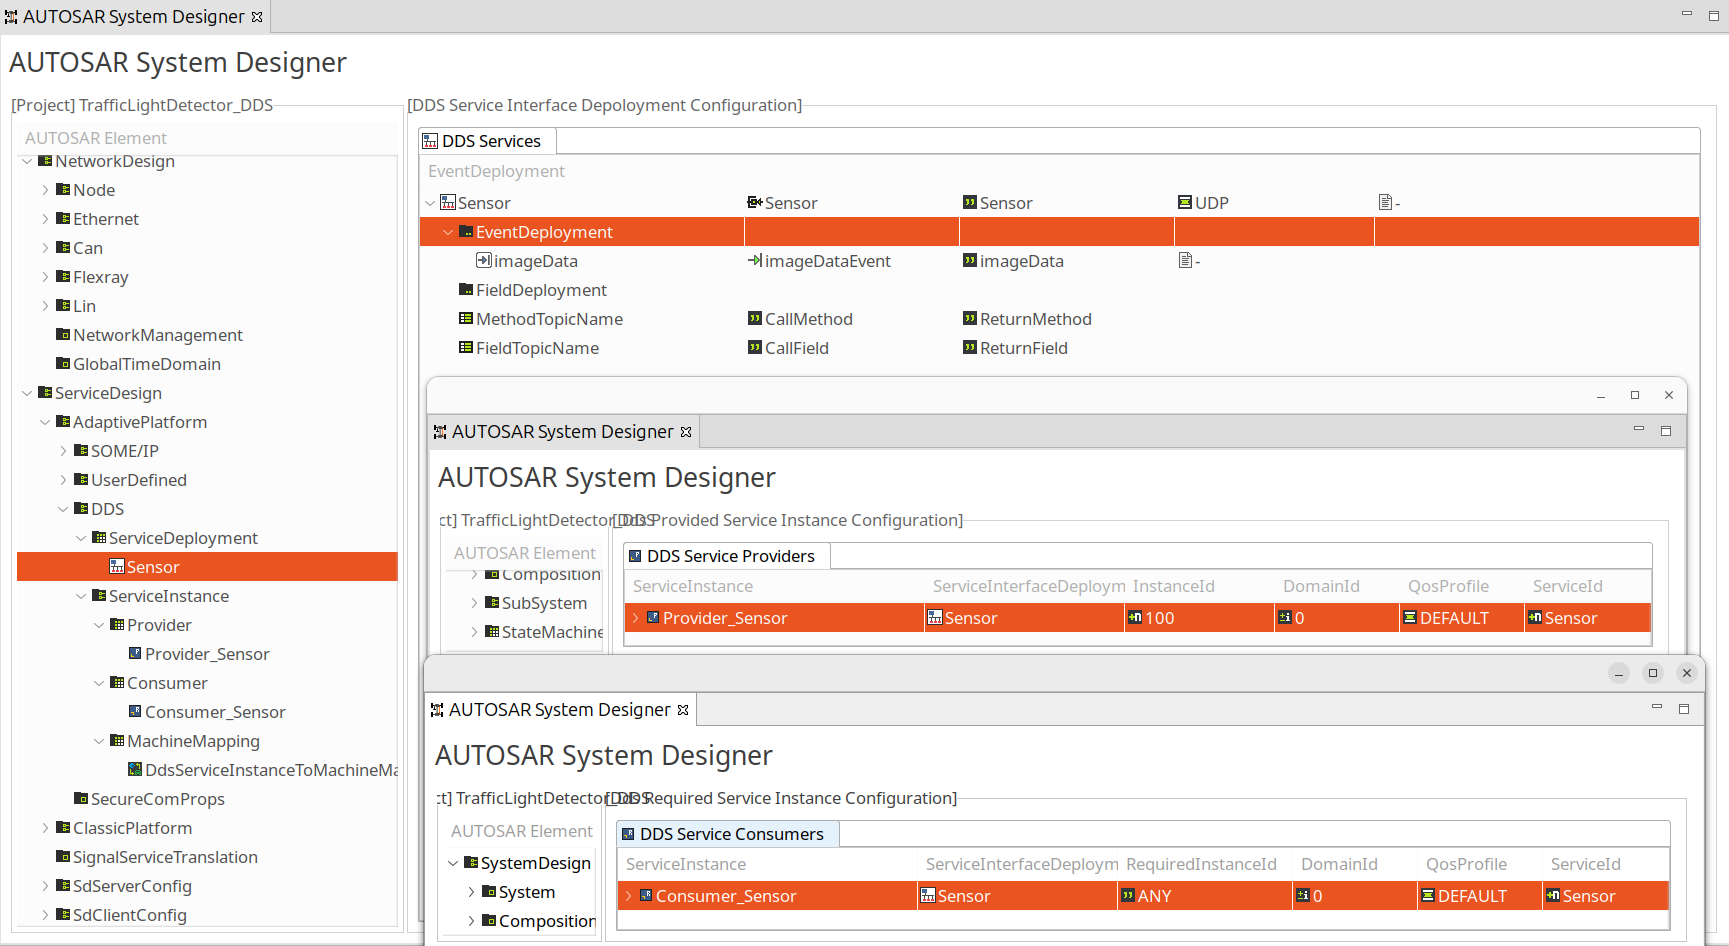
\includegraphics[width=0.75\textwidth]{Images/chap3/image_methodology/serviceInterfaceDesign/DDS_Config.png}
    \vspace{0.5cm}
    \caption{Mapping Service Instances to Machine Network Endpoint}
    \label{fig:dds_config}
\end{figure}

Similarly to the SOME/IP configuration, Figure~\ref{fig:dds_config} presents the DDS-based deployment configuration used for the \texttt{Sensor} service. In the DDS Service Interface Deployment Configuration, the service interface is deployed with the \texttt{imageDataEvent} event and the corresponding DDS topic \texttt{imageData}. The event deployment is configured to use UDP transport, allowing the Provider and Client applications to exchange image and metadata payloads through DDS publish/subscribe communication.

The provided service instance is configured as \texttt{Provider\_Sensor}, bound to the \texttt{Sensor} service deployment with instance-id~\texttt{100}, DDS Domain Id~\texttt{0}, and the \texttt{DEFAULT} QoS profile. The required service instance is configured as \texttt{Consumer\_Sensor}, also bound to the same \texttt{Sensor} service deployment, but with required instance-id~\texttt{ANY}. This configuration allows the Client application to discover and subscribe to the Provider service instance dynamically within the same DDS domain.

Through this DDS configuration, the abstract AUTOSAR service definition is mapped to concrete DDS communication entities, including service deployment, topic, event, provider instance, consumer instance, domain identifier, and QoS profile. This mapping is essential for the implemented prototype because the runtime communication between \texttt{ProviderSensor} and \texttt{ClientSensor} is realized through DDS rather than SOME/IP. As a result, the system can publish \texttt{imageDataEvent} samples on the \texttt{imageData} topic and deliver the \texttt{GpsJpegWireHeader + JPEG} payload from the Provider to the Client in a service-oriented and configurable manner.

\subsubsection{Application Design}

% Modeling Adaptive Application
\begin{figure}[H]
    \centering
    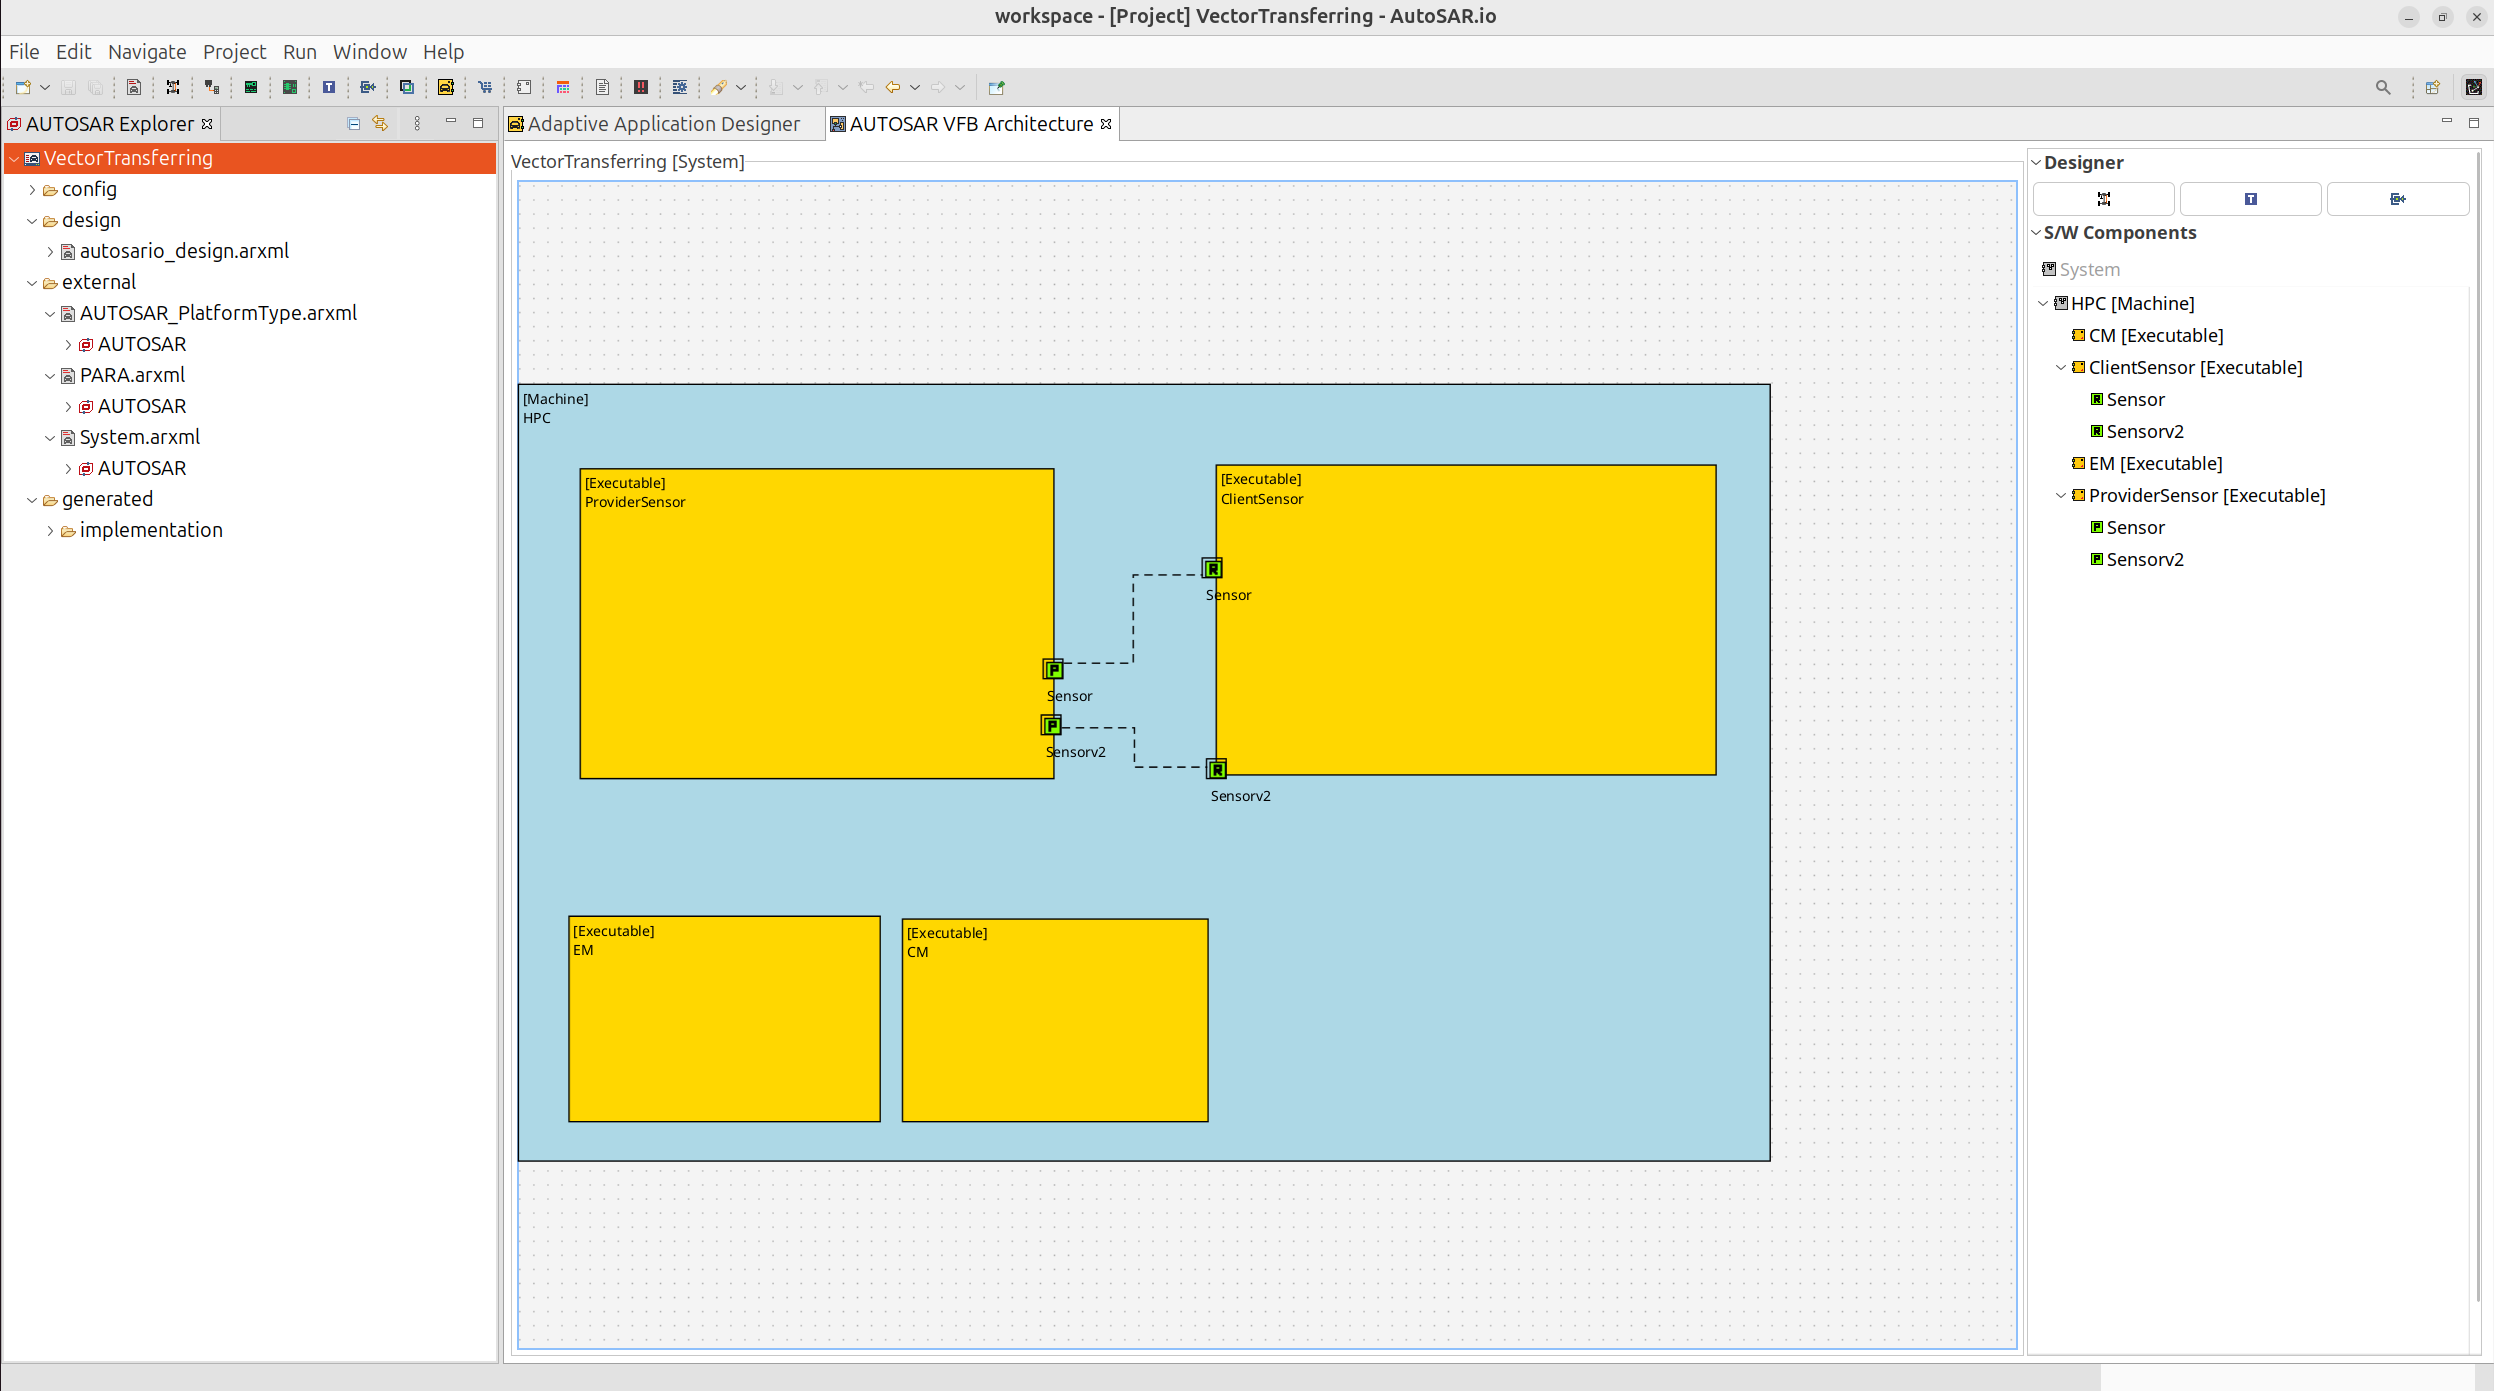
\includegraphics[width=0.75\textwidth]{Images/chap3/image_methodology/applicationDesign/modelingApplication.png}
    \vspace{0.5cm}
    \caption{Modeling of Adaptive Application}
    \label{fig:modeling_application}
\end{figure}

Figure~\ref{fig:modeling_application} shows the Adaptive Application modeling view, where users define the overall application architecture by assigning application executables to a specific machine. In this workspace, the target machine \texttt{HPC} is selected as the deployment context, and multiple executables such as \texttt{ProviderSensor}, \texttt{ClientSensor}, \texttt{CM}, and \texttt{EM} are instantiated within it. Logical connections between executables are visually represented through ports, allowing designers to describe interaction relationships at the architectural level. This model serves as a central design step that links application executables with the underlying machine, providing a clear and structured representation of how software components are organized and deployed in an Adaptive AUTOSAR system.


% Configure Provider Executable Properties
\begin{figure}[H]
    \centering
    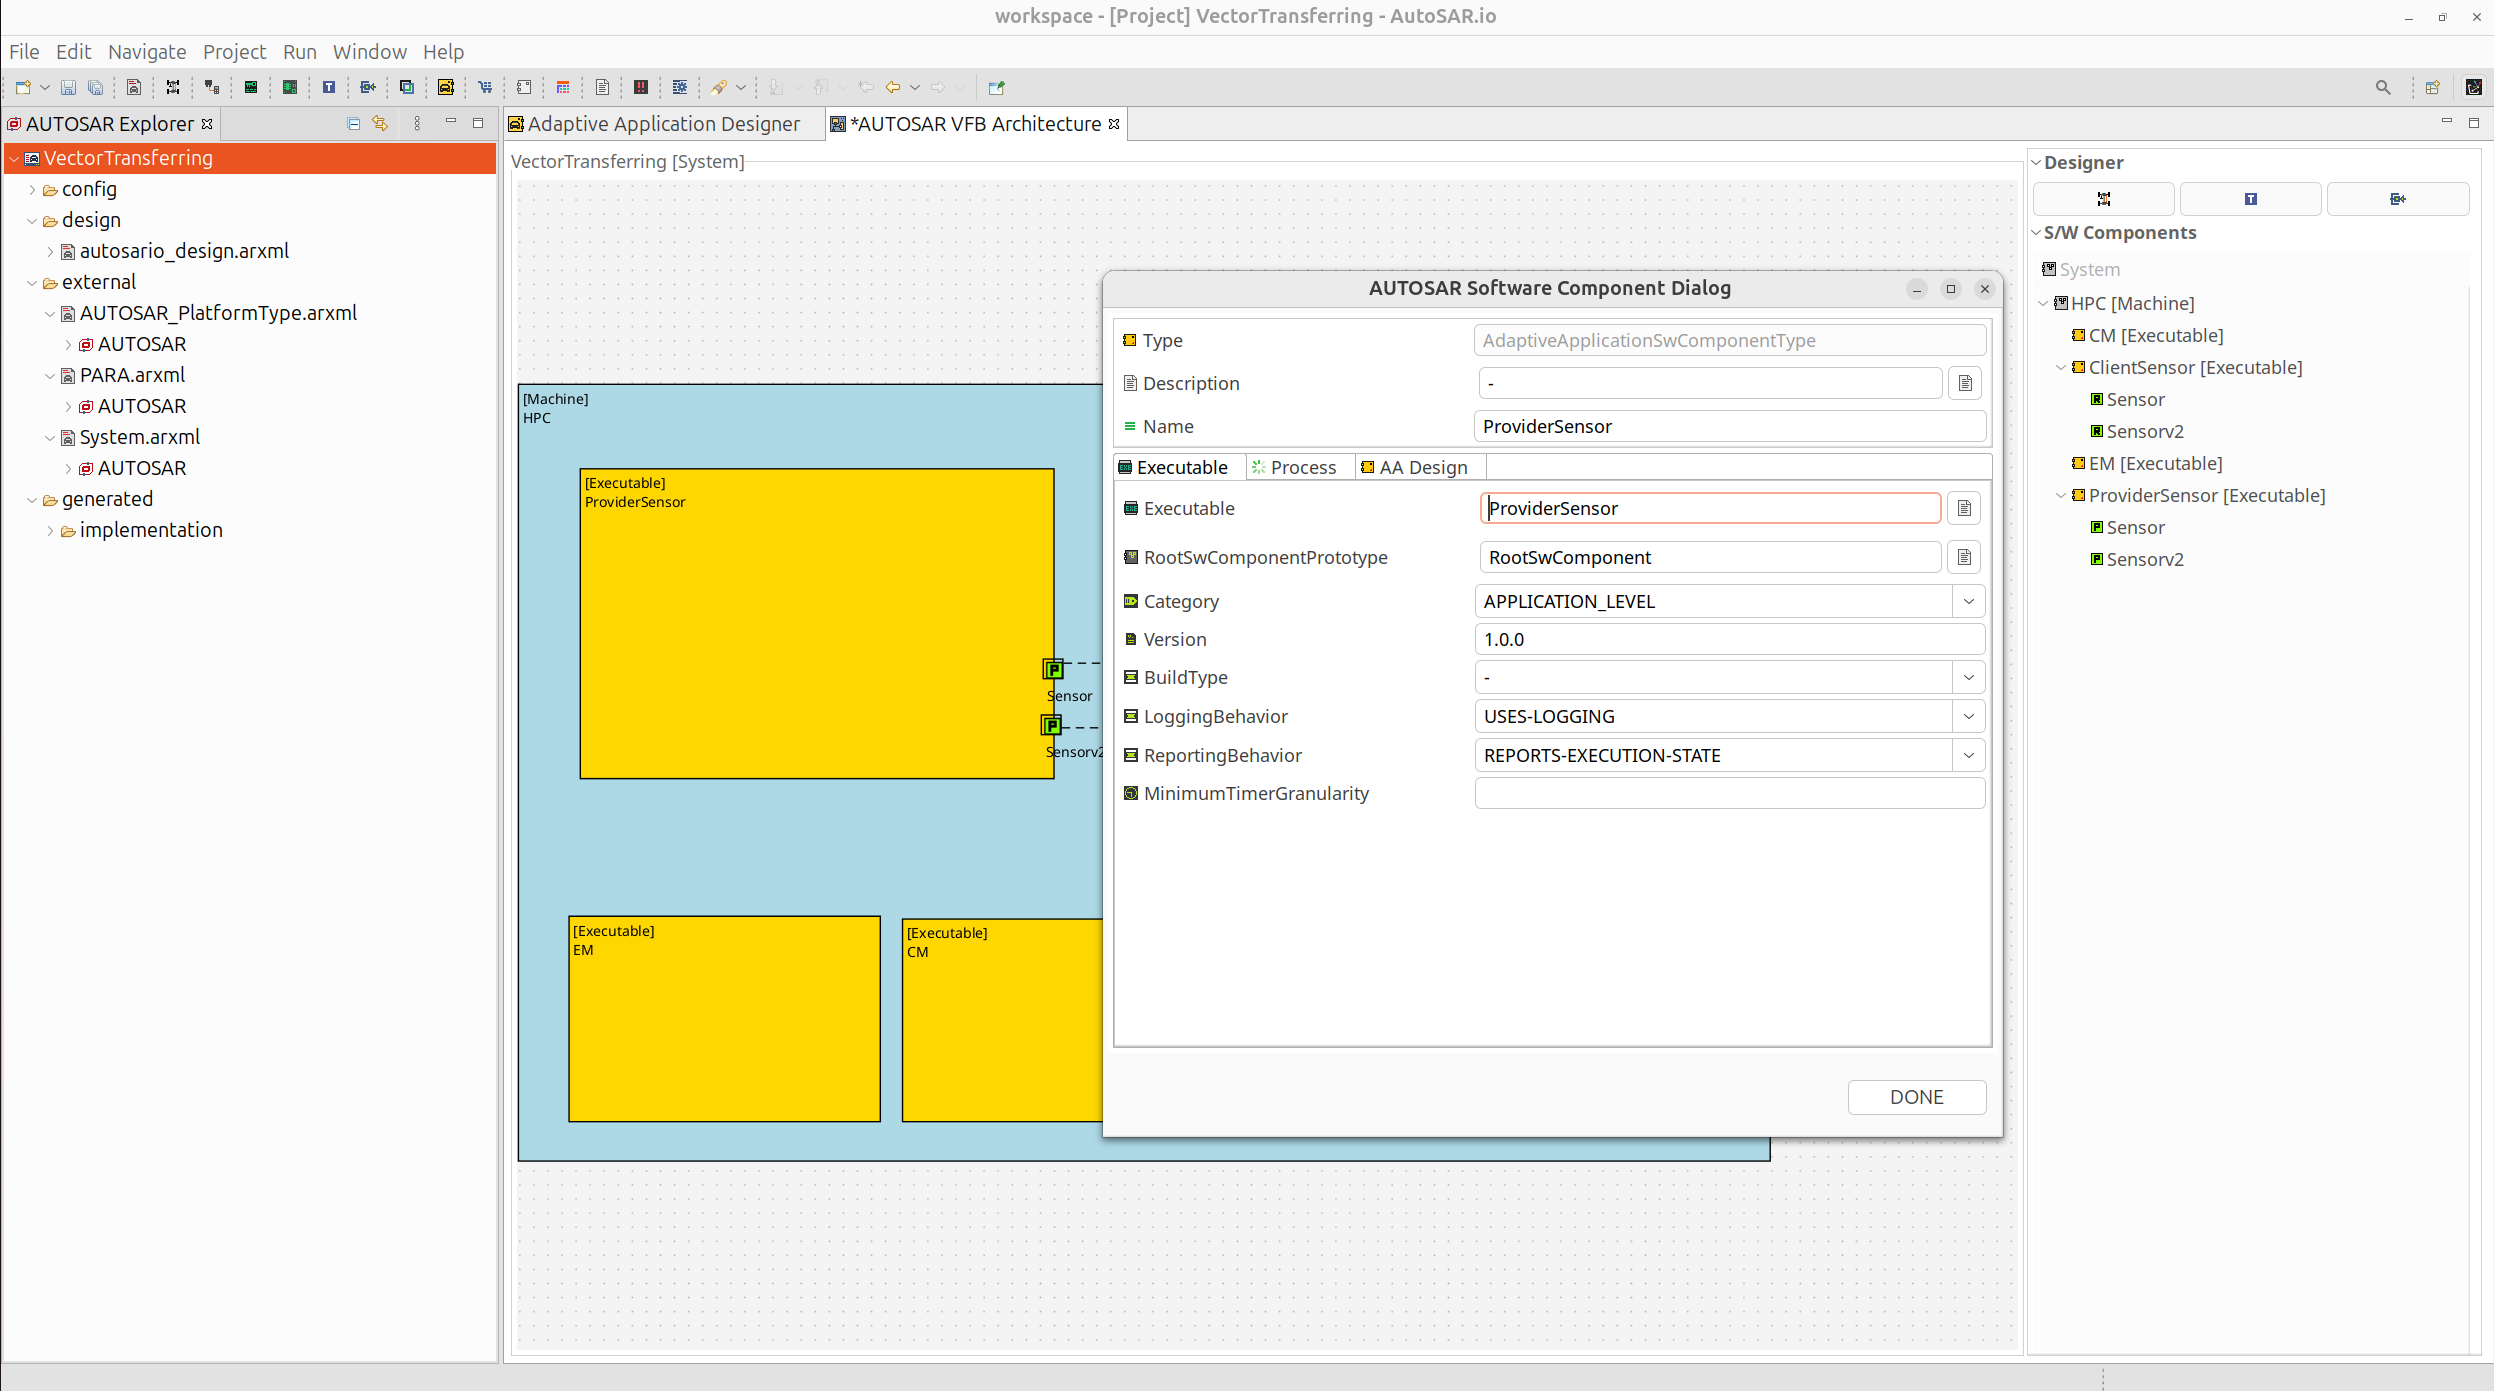
\includegraphics[width=0.75\textwidth]{Images/chap3/image_methodology/applicationDesign/providerExProperties.png}
    \vspace{0.5cm}
    \caption{Configuration of Provider Executable Properties}
    \label{fig:app_provider_executable_properties}
\end{figure}

Figure~\ref{fig:app_provider_executable_properties} presents the configuration of the provider application executable within the Adaptive Application Designer. In this view, the executable \texttt{ProviderSensor} is defined as an application level software component with a specific version and logging behavior. Key properties such as execution category, reporting behavior, and minimum timer granularity are configured to control runtime characteristics and observability. By assigning these attributes, the provider executable is clearly identified as a service offering entity and is prepared to integrate with the Adaptive AUTOSAR execution environment in a consistent and manageable manner.

% Map Provider Ports to Service Interface
\begin{figure}[H]
    \centering
    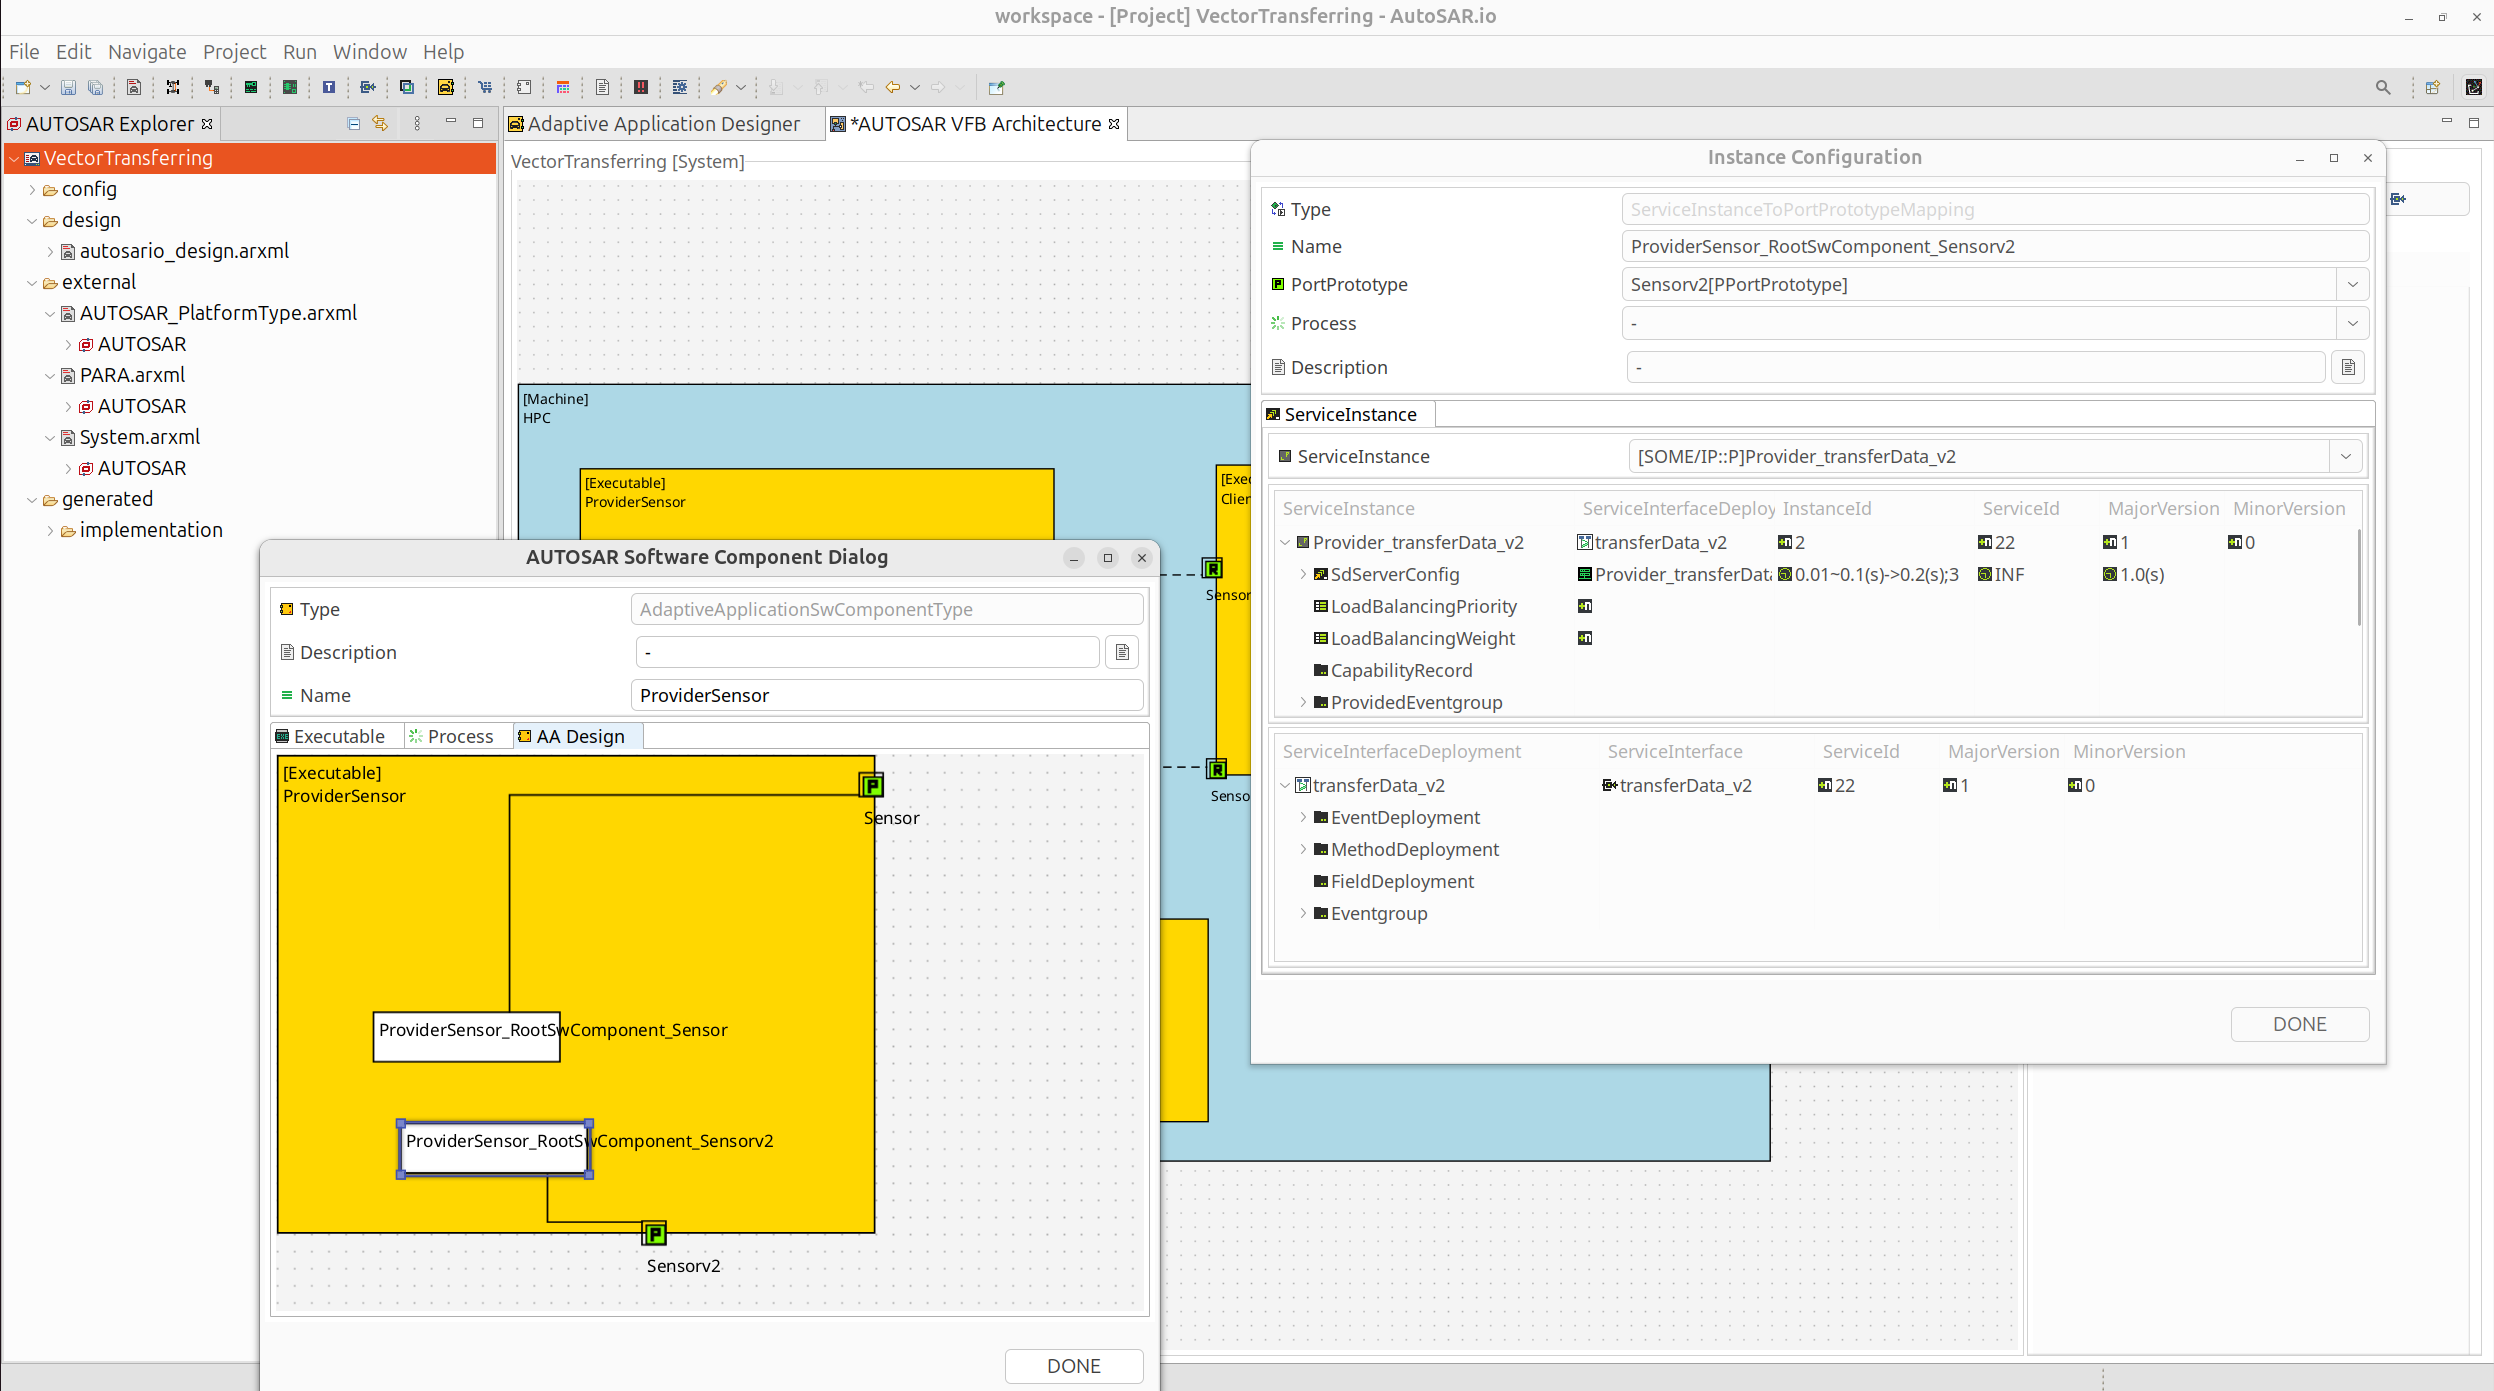
\includegraphics[width=0.75\textwidth]{Images/chap3/image_methodology/applicationDesign/mappingPortProviderEx.png}
    \vspace{0.5cm}
    \caption{Mapping Provider Ports to Service Interface}
    \label{fig:app_mapping_provider_ports}
\end{figure}

Figure~\ref{fig:app_mapping_provider_ports} illustrates the association between the provider executable ports and the previously defined AUTOSAR software component. In this step, the ports of the \texttt{ProviderSensor} executable are mapped to the corresponding port prototypes of the Adaptive Application Software Component that has already been specified in the AUTOSAR model. This configuration establishes a clear link between the executable instance and its software component definition, ensuring that the executable correctly realizes the component’s provided interfaces. As a result, the application implementation becomes consistent with the AUTOSAR architectural model before being bound to concrete service instances and communication middleware.


% Configure Subscriber Executable Properties
\begin{figure}[H]
    \centering
    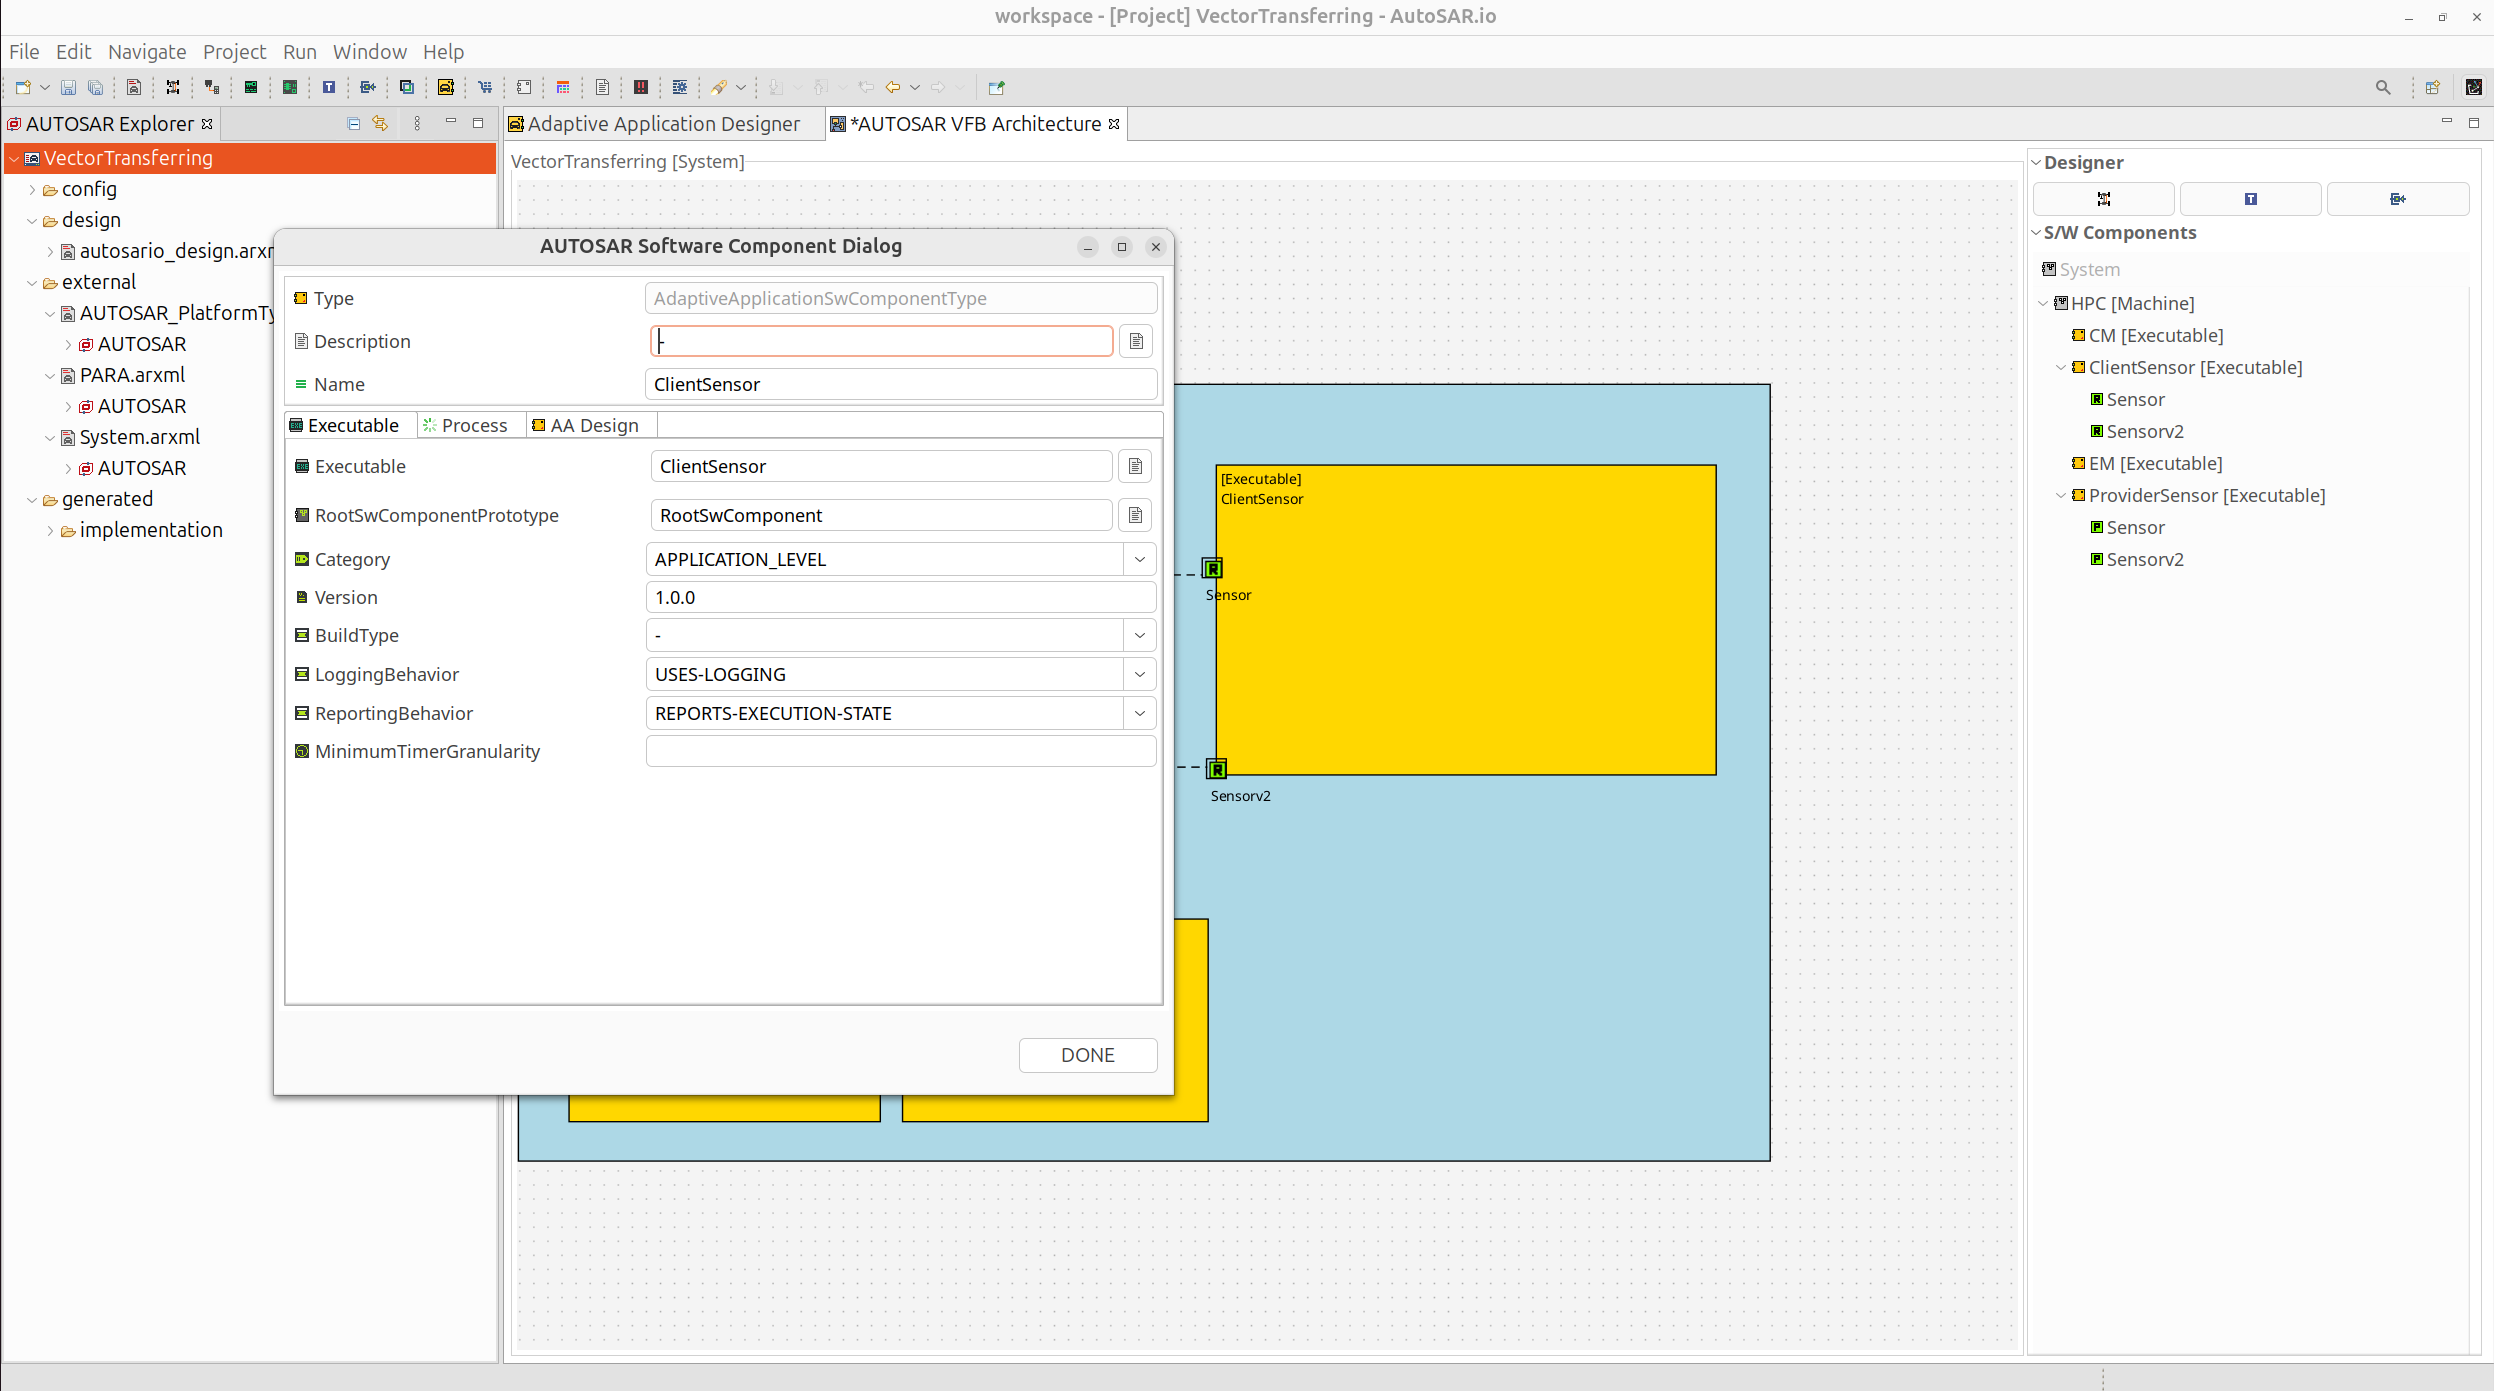
\includegraphics[width=0.75\textwidth]{Images/chap3/image_methodology/applicationDesign/subscriberExProperties.png}
    \vspace{0.5cm}
    \caption{Configuration of Subscriber Executable Properties}
    \label{fig:app_subscriber_executable_properties}
\end{figure}

Figure~\ref{fig:app_subscriber_executable_properties} illustrates the definition of the \texttt{ClientSensor} executable as an adaptive application software component. In this step, the executable is characterized at the application level by specifying its name, version, category, and runtime behavior such as logging and execution state reporting. This configuration formally registers the client application in the AUTOSAR model and establishes it as a runnable entity that can participate in service oriented communication.

% Map Client Ports to Service Interface
\begin{figure}[H]
    \centering
    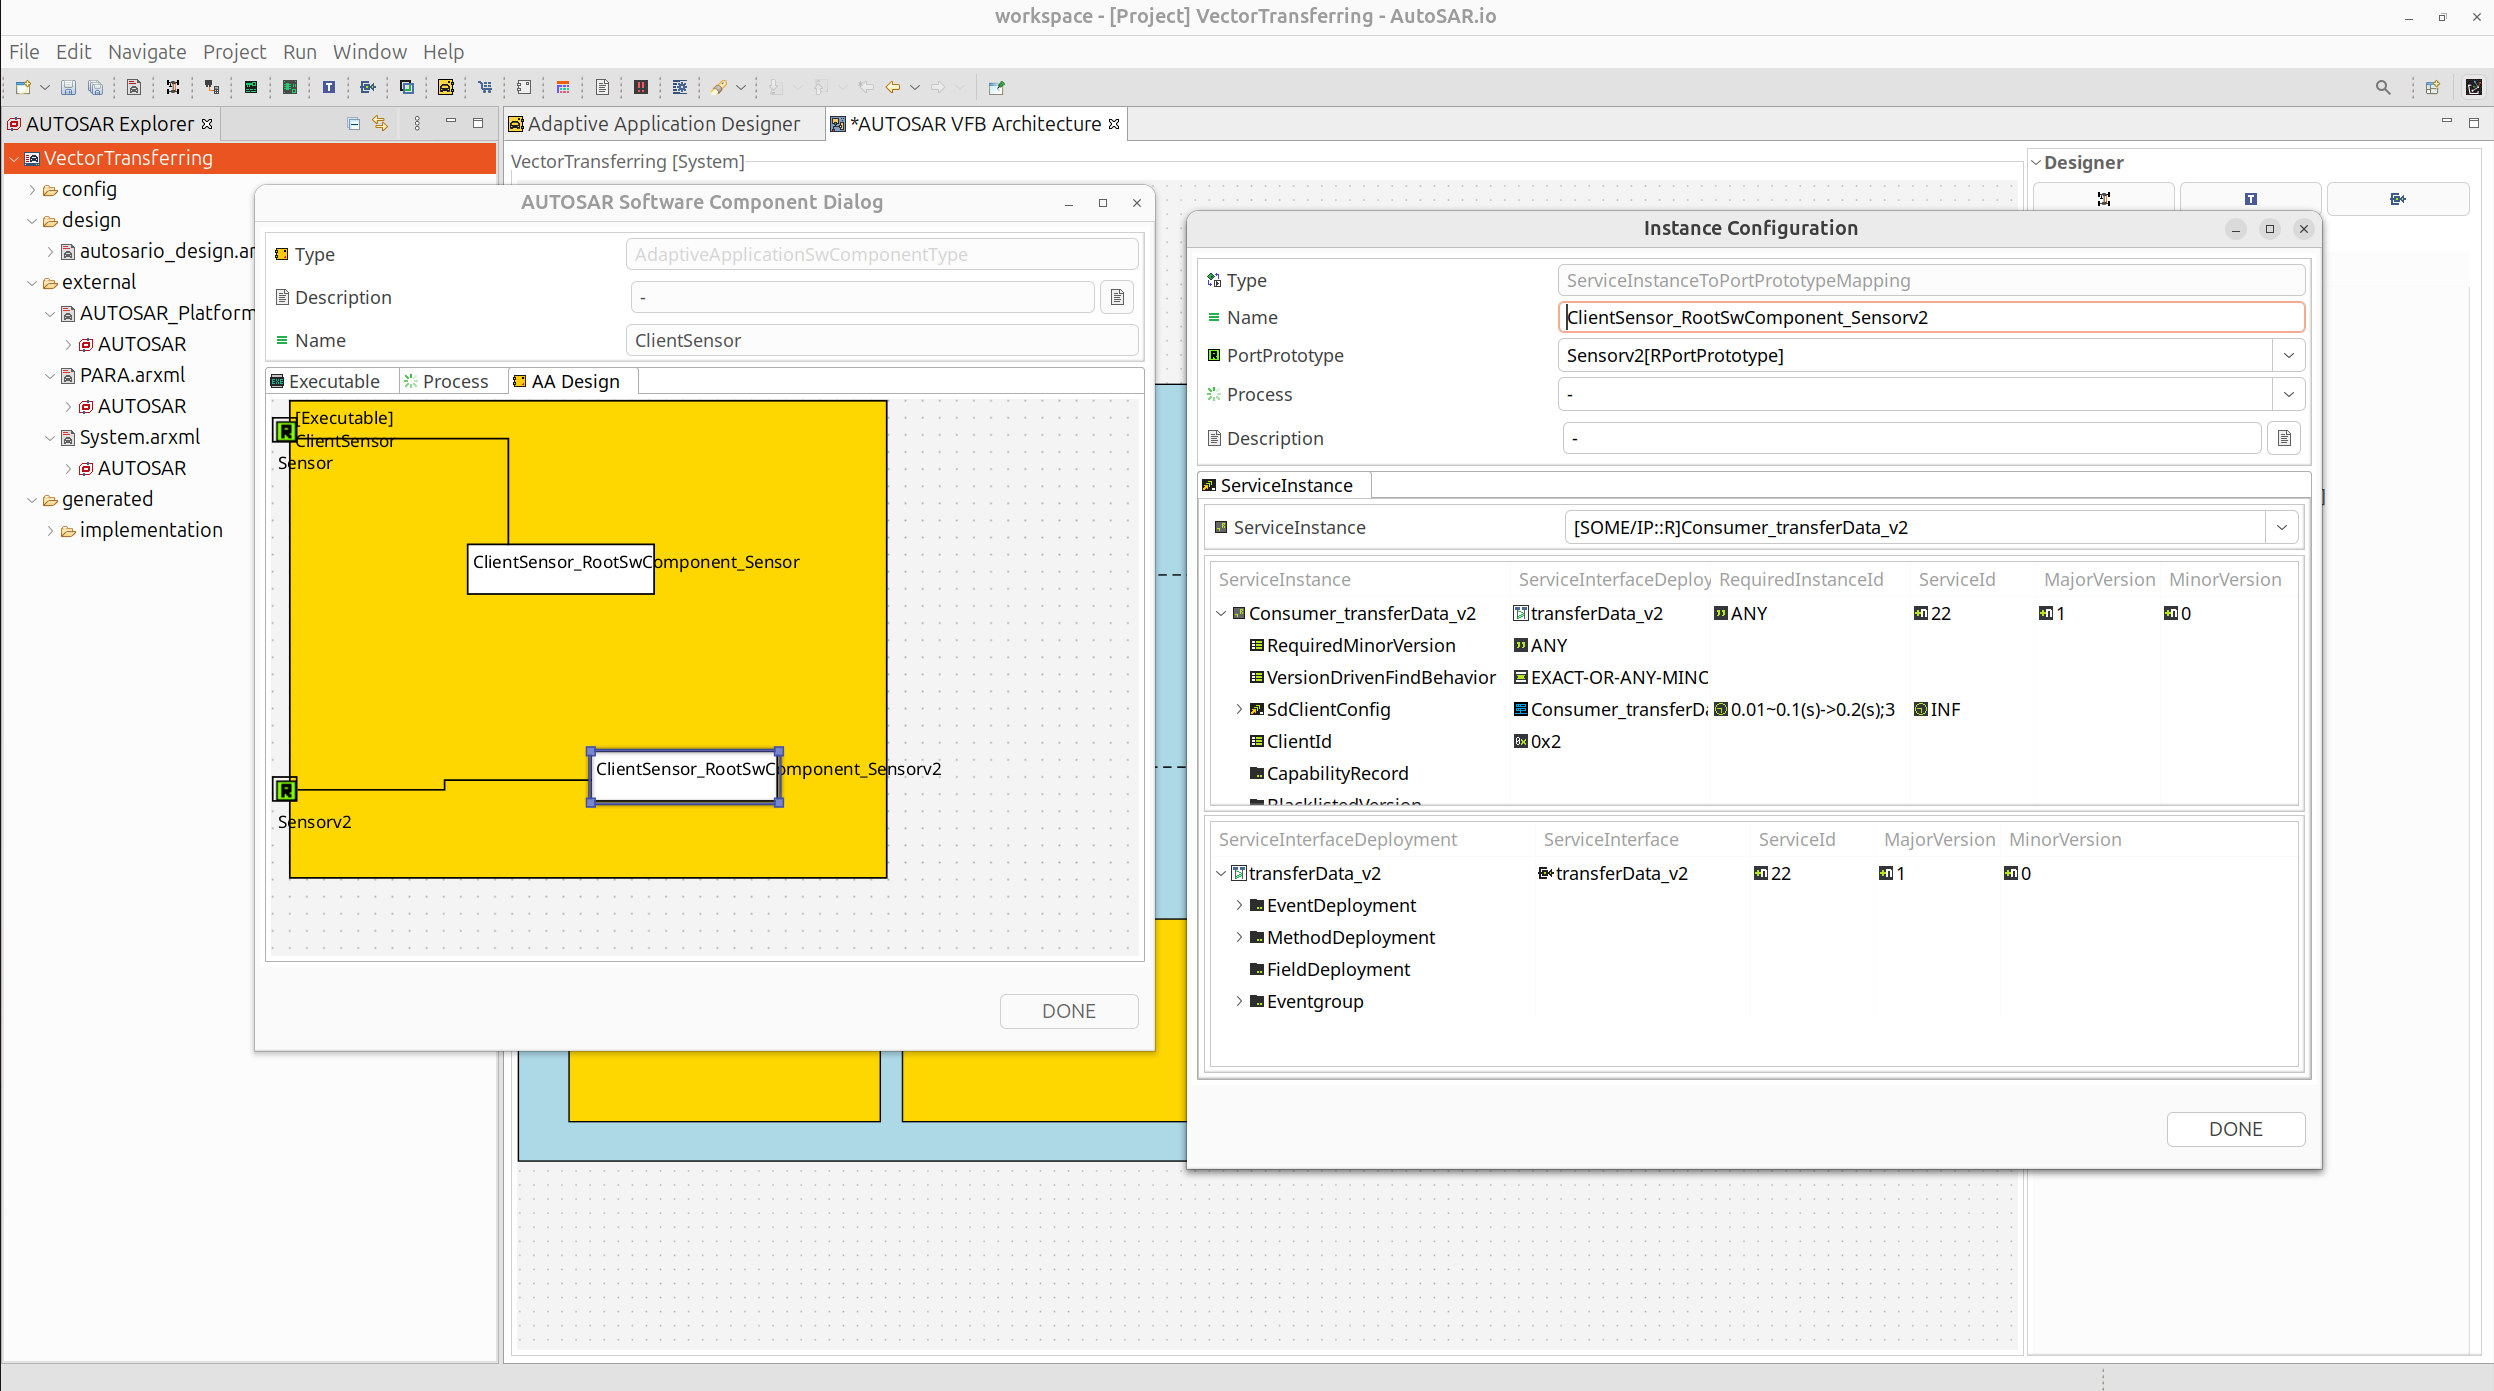
\includegraphics[width=0.75\textwidth]{Images/chap3/image_methodology/applicationDesign/mappingPortClientEx.png}
    \vspace{0.5cm}
    \caption{Mapping Client Ports to Service Interface}
    \label{fig:app_mapping_client_ports}
\end{figure}

As shown in Figure~\ref{fig:app_mapping_client_ports}, the required ports of the \texttt{ClientSensor} software component are then associated with the corresponding port prototypes defined in the AUTOSAR architecture. This association links the client implementation to the abstract interface contracts specified at design time, without directly binding it to network level details. By completing this step, the client executable is structurally aligned with the AUTOSAR software component model, enabling subsequent binding to concrete service instances during service deployment and machine mapping.

% Configure Application Startup Behavior
\begin{figure}[H]
    \centering
    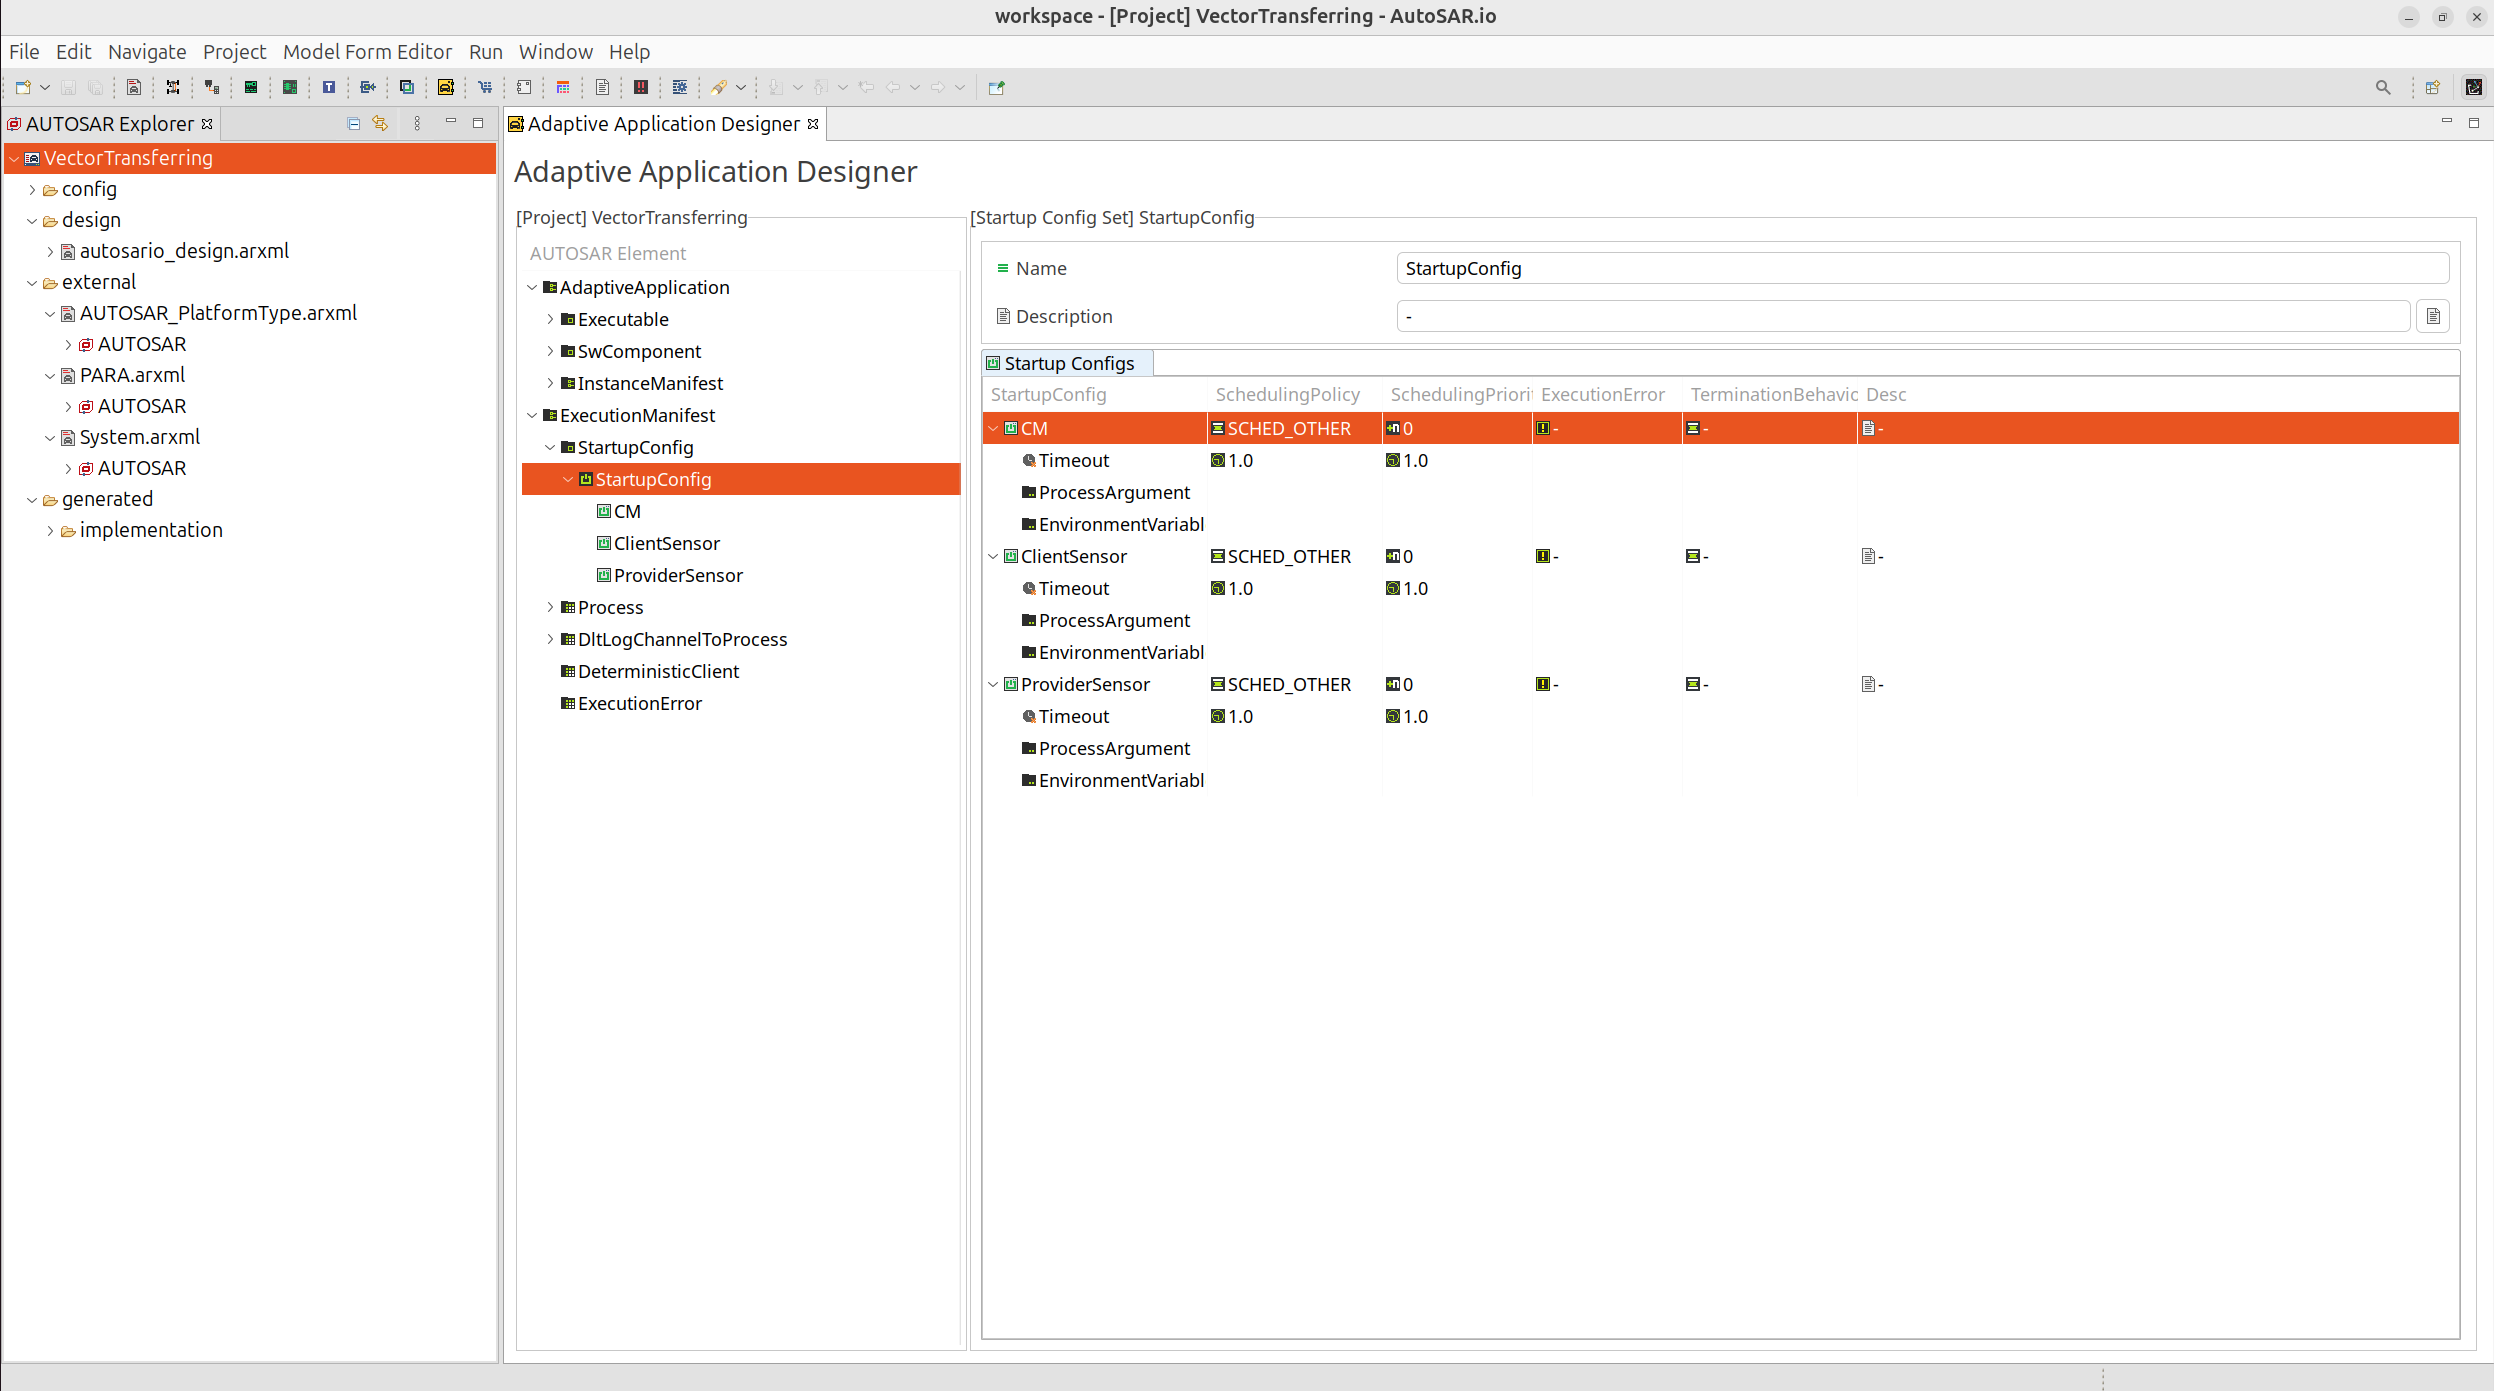
\includegraphics[width=0.75\textwidth]{Images/chap3/image_methodology/applicationDesign/configureStartupConfigure.png}
    \vspace{0.5cm}
    \caption{Configuration of Application Startup Behavior}
    \label{fig:app_startup_configuration}
\end{figure}

Figure~\ref{fig:app_startup_configuration} illustrates the startup configuration set that governs how adaptive application processes are initialized on the target platform. Each process, including \texttt{CM}, \texttt{ClientSensor}, and \texttt{ProviderSensor}, is assigned a scheduling policy and priority, ensuring consistent execution behavior under the POSIX based operating environment. The use of a unified scheduling class allows the platform to manage multiple applications in a predictable manner during system boot.

In addition, the startup configuration defines timeout values and process level parameters that control execution supervision at launch time. By explicitly specifying these attributes, the system ensures that all applications enter a well defined initial state and comply with platform execution constraints. This configuration plays a critical role in coordinating application startup with function group transitions and provides a stable foundation for subsequent runtime interactions.

% Bind DLT Channels to Application Processes
\begin{figure}[H]
    \centering
    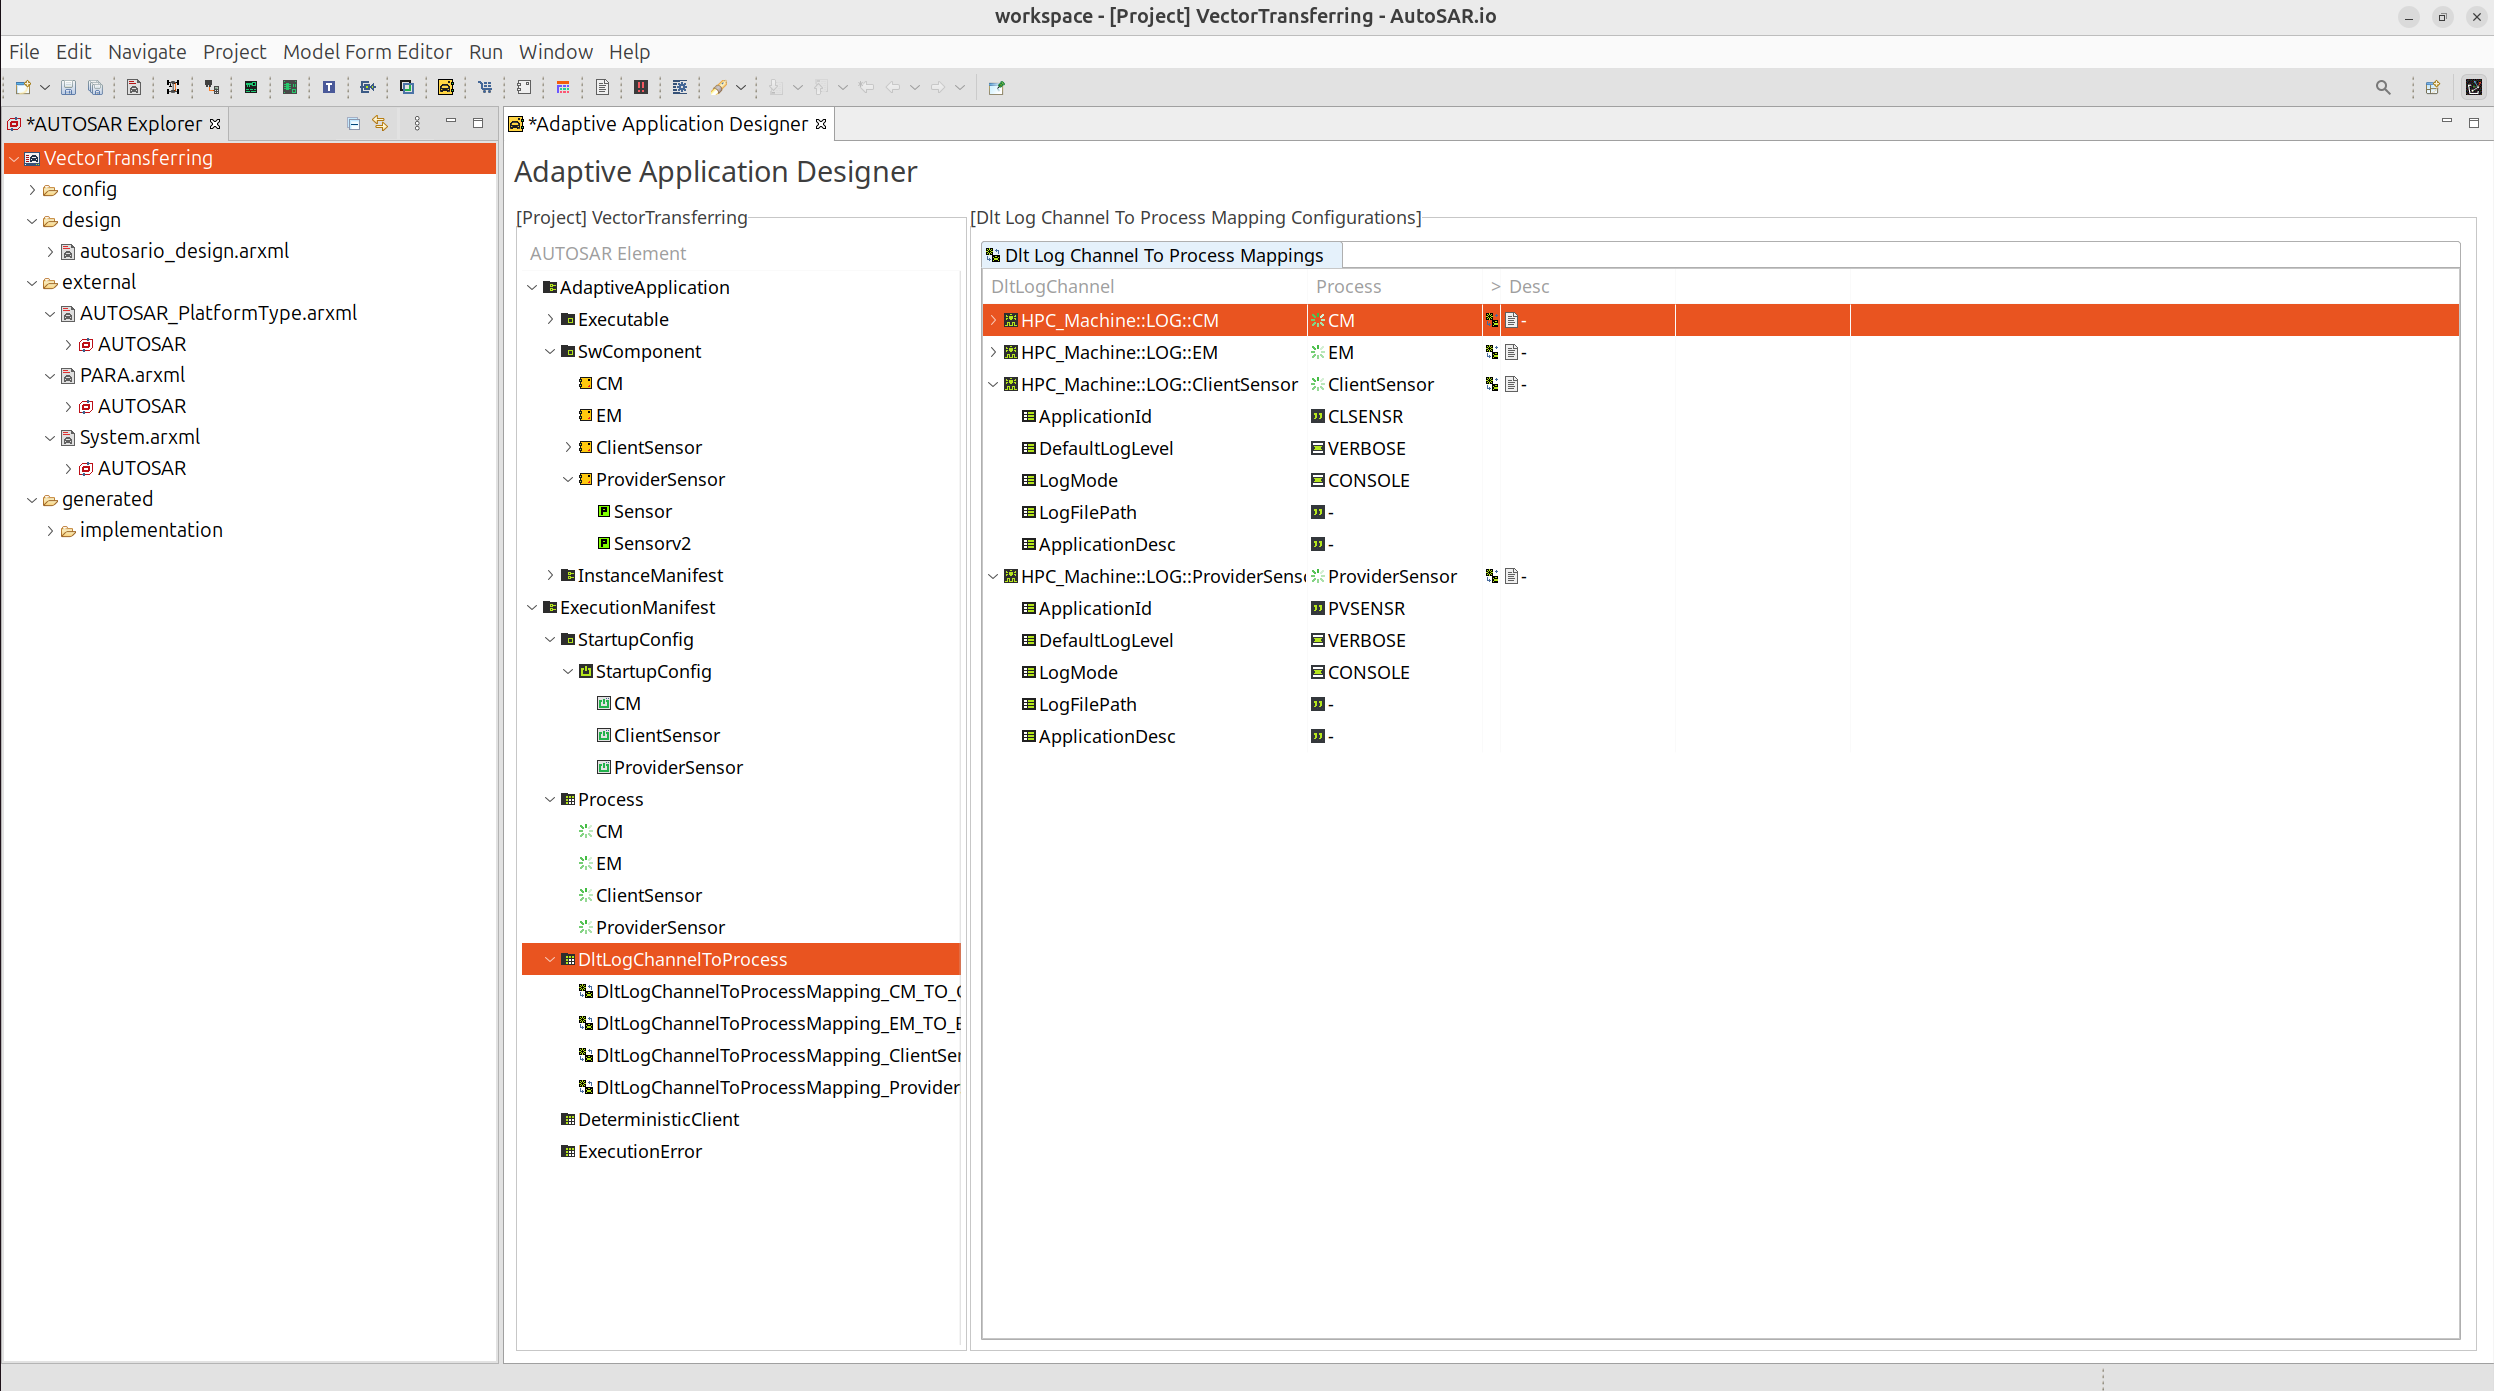
\includegraphics[width=0.75\textwidth]{Images/chap3/image_methodology/applicationDesign/configureDLTChanneltoProcess.png}
    \vspace{0.5cm}
    \caption{Binding Diagnostic Log and Trace Channels to Application Processes}
    \label{fig:app_dlt_process_mapping}
\end{figure}

Figure~\ref{fig:app_dlt_process_mapping} depicts the association between Diagnostic Log and Trace channels and individual application processes. Each process is connected to a specific DLT channel with defined log levels and output modes, enabling consistent monitoring and debugging at runtime. This mapping ensures that diagnostic information is traceable per application, which supports efficient analysis and maintenance in Adaptive AUTOSAR deployments.

% Configure Provider Application Process
\begin{figure}[H]
    \centering
    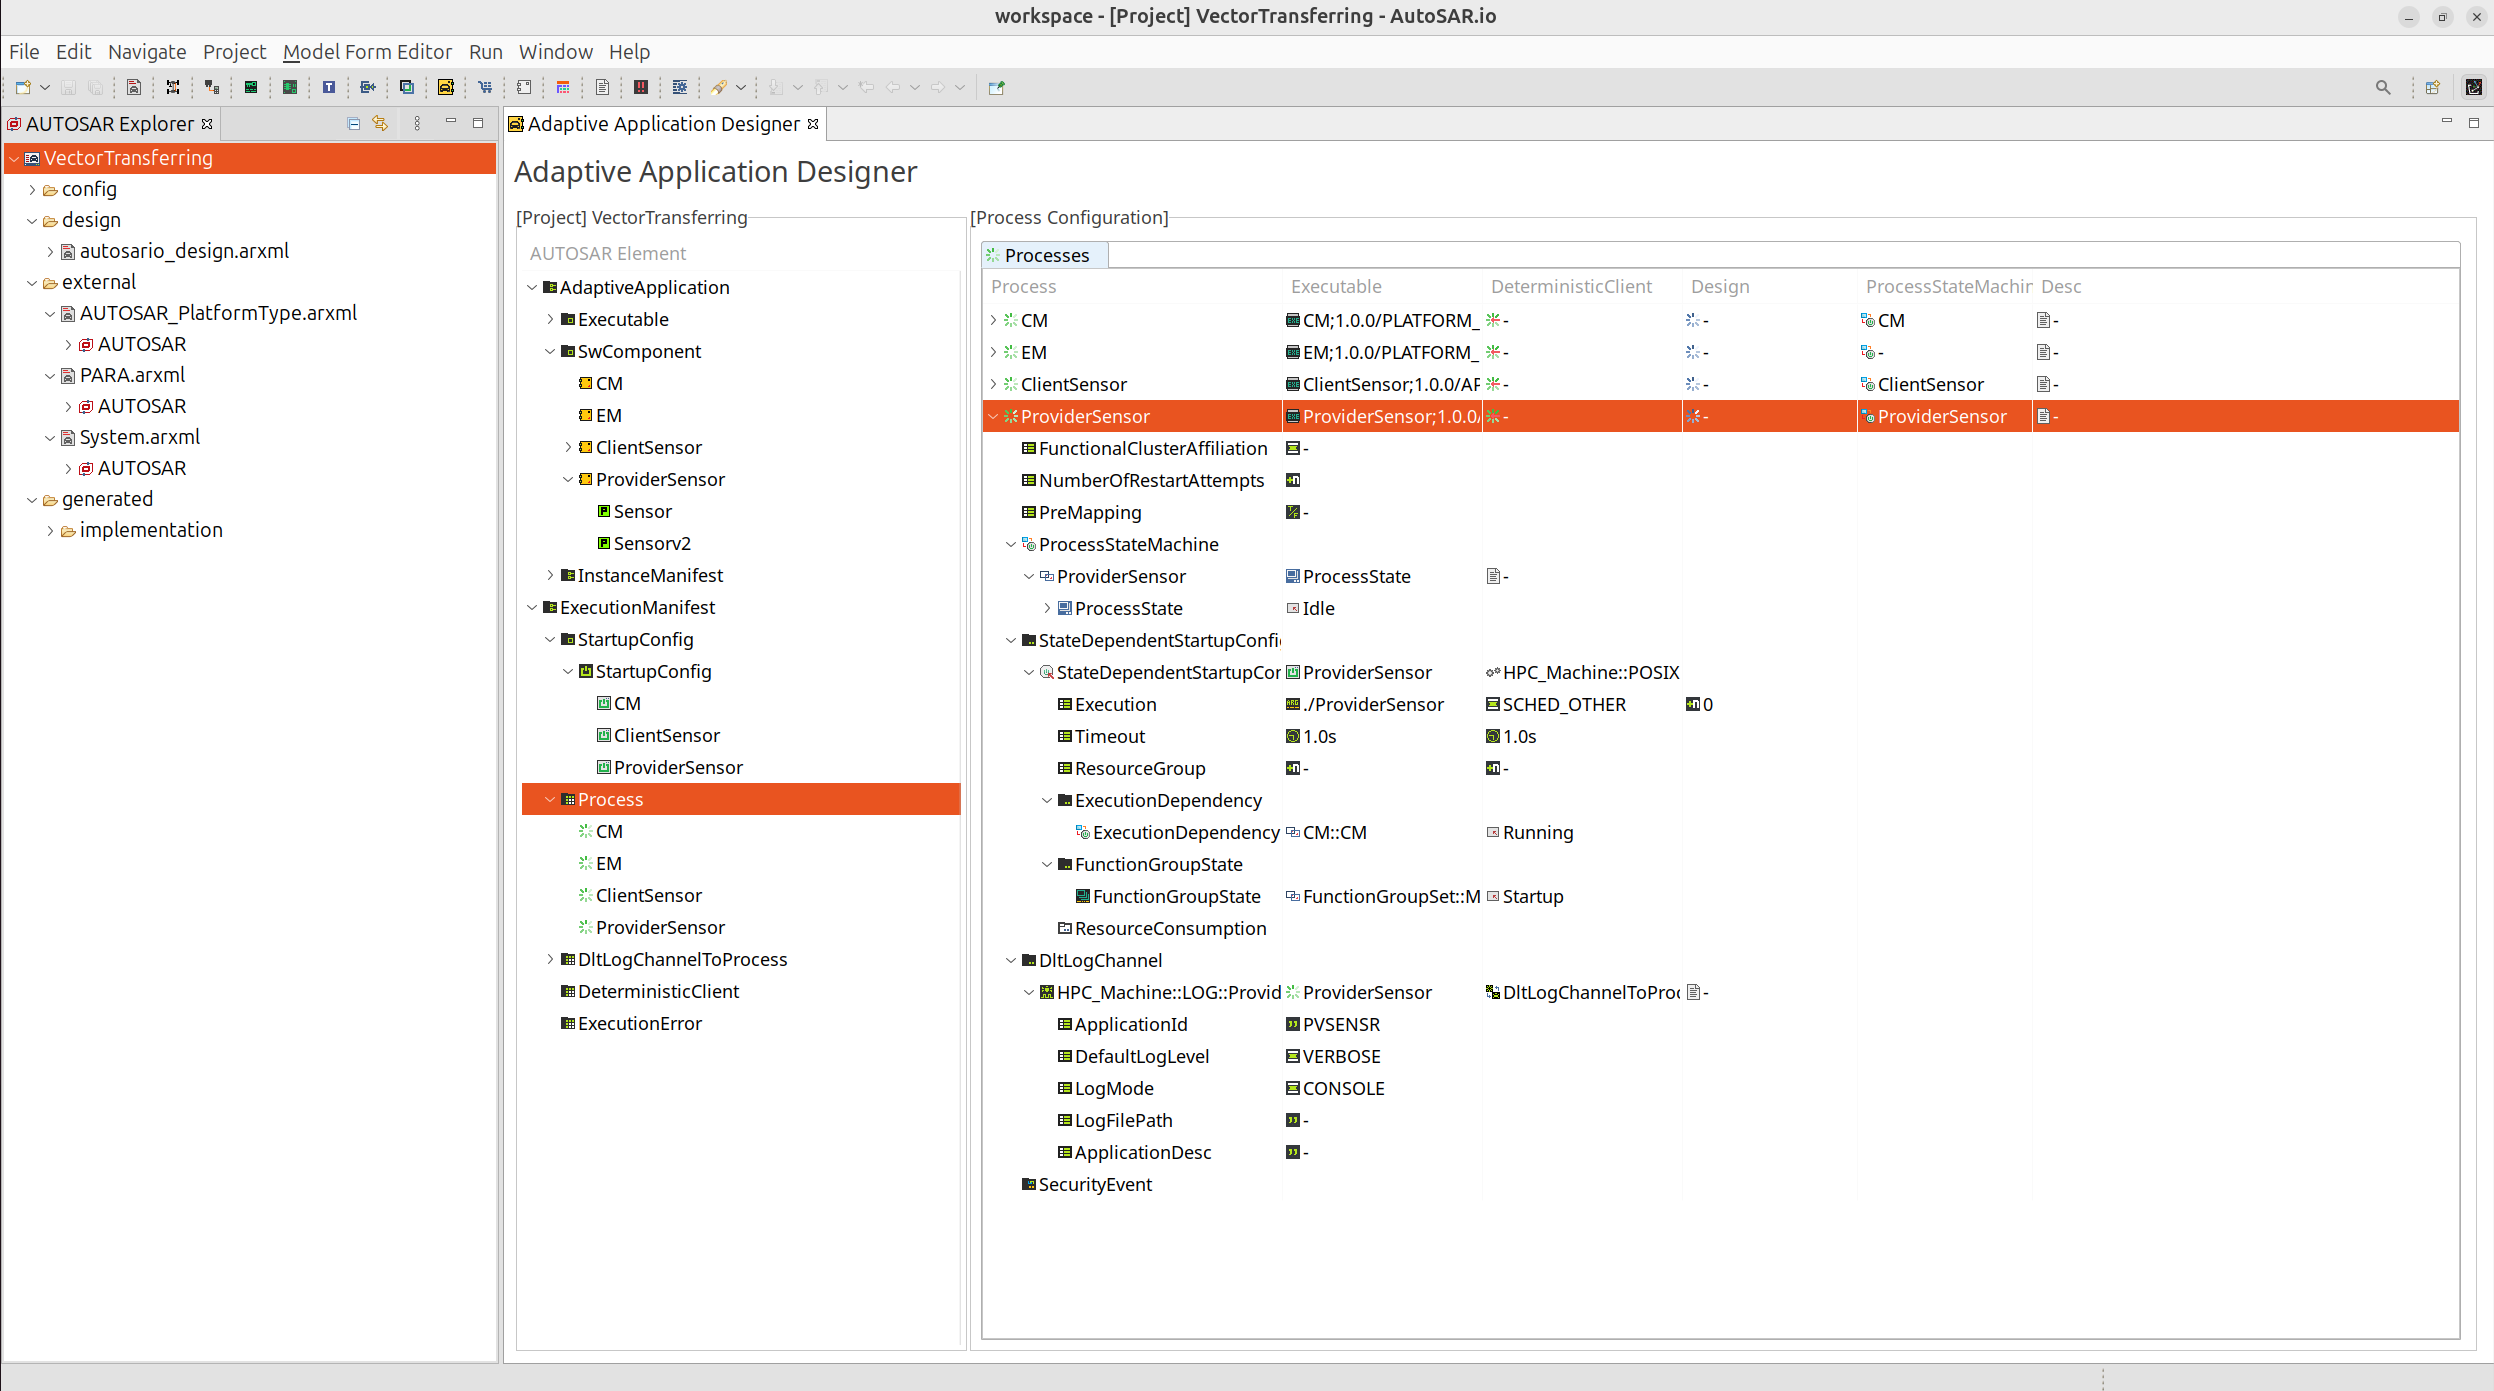
\includegraphics[width=0.75\textwidth]{Images/chap3/image_methodology/applicationDesign/configureProviderProcess.png}
    \vspace{0.5cm}
    \caption{Configuration of Provider Application Process}
    \label{fig:app_provider_process_configuration}
\end{figure}

As illustrated in Figure~\ref{fig:app_provider_process_configuration}, the provider application process is configured by linking the \texttt{ProviderSensor} executable to a dedicated process entity. This step specifies process level attributes such as restart policy, execution dependency, and state machine association, which together describe how the provider behaves during runtime transitions. The configuration clarifies the provider’s role in the execution flow and its dependency on platform level services.

% Configure Client Application Process
\begin{figure}[H]
    \centering
    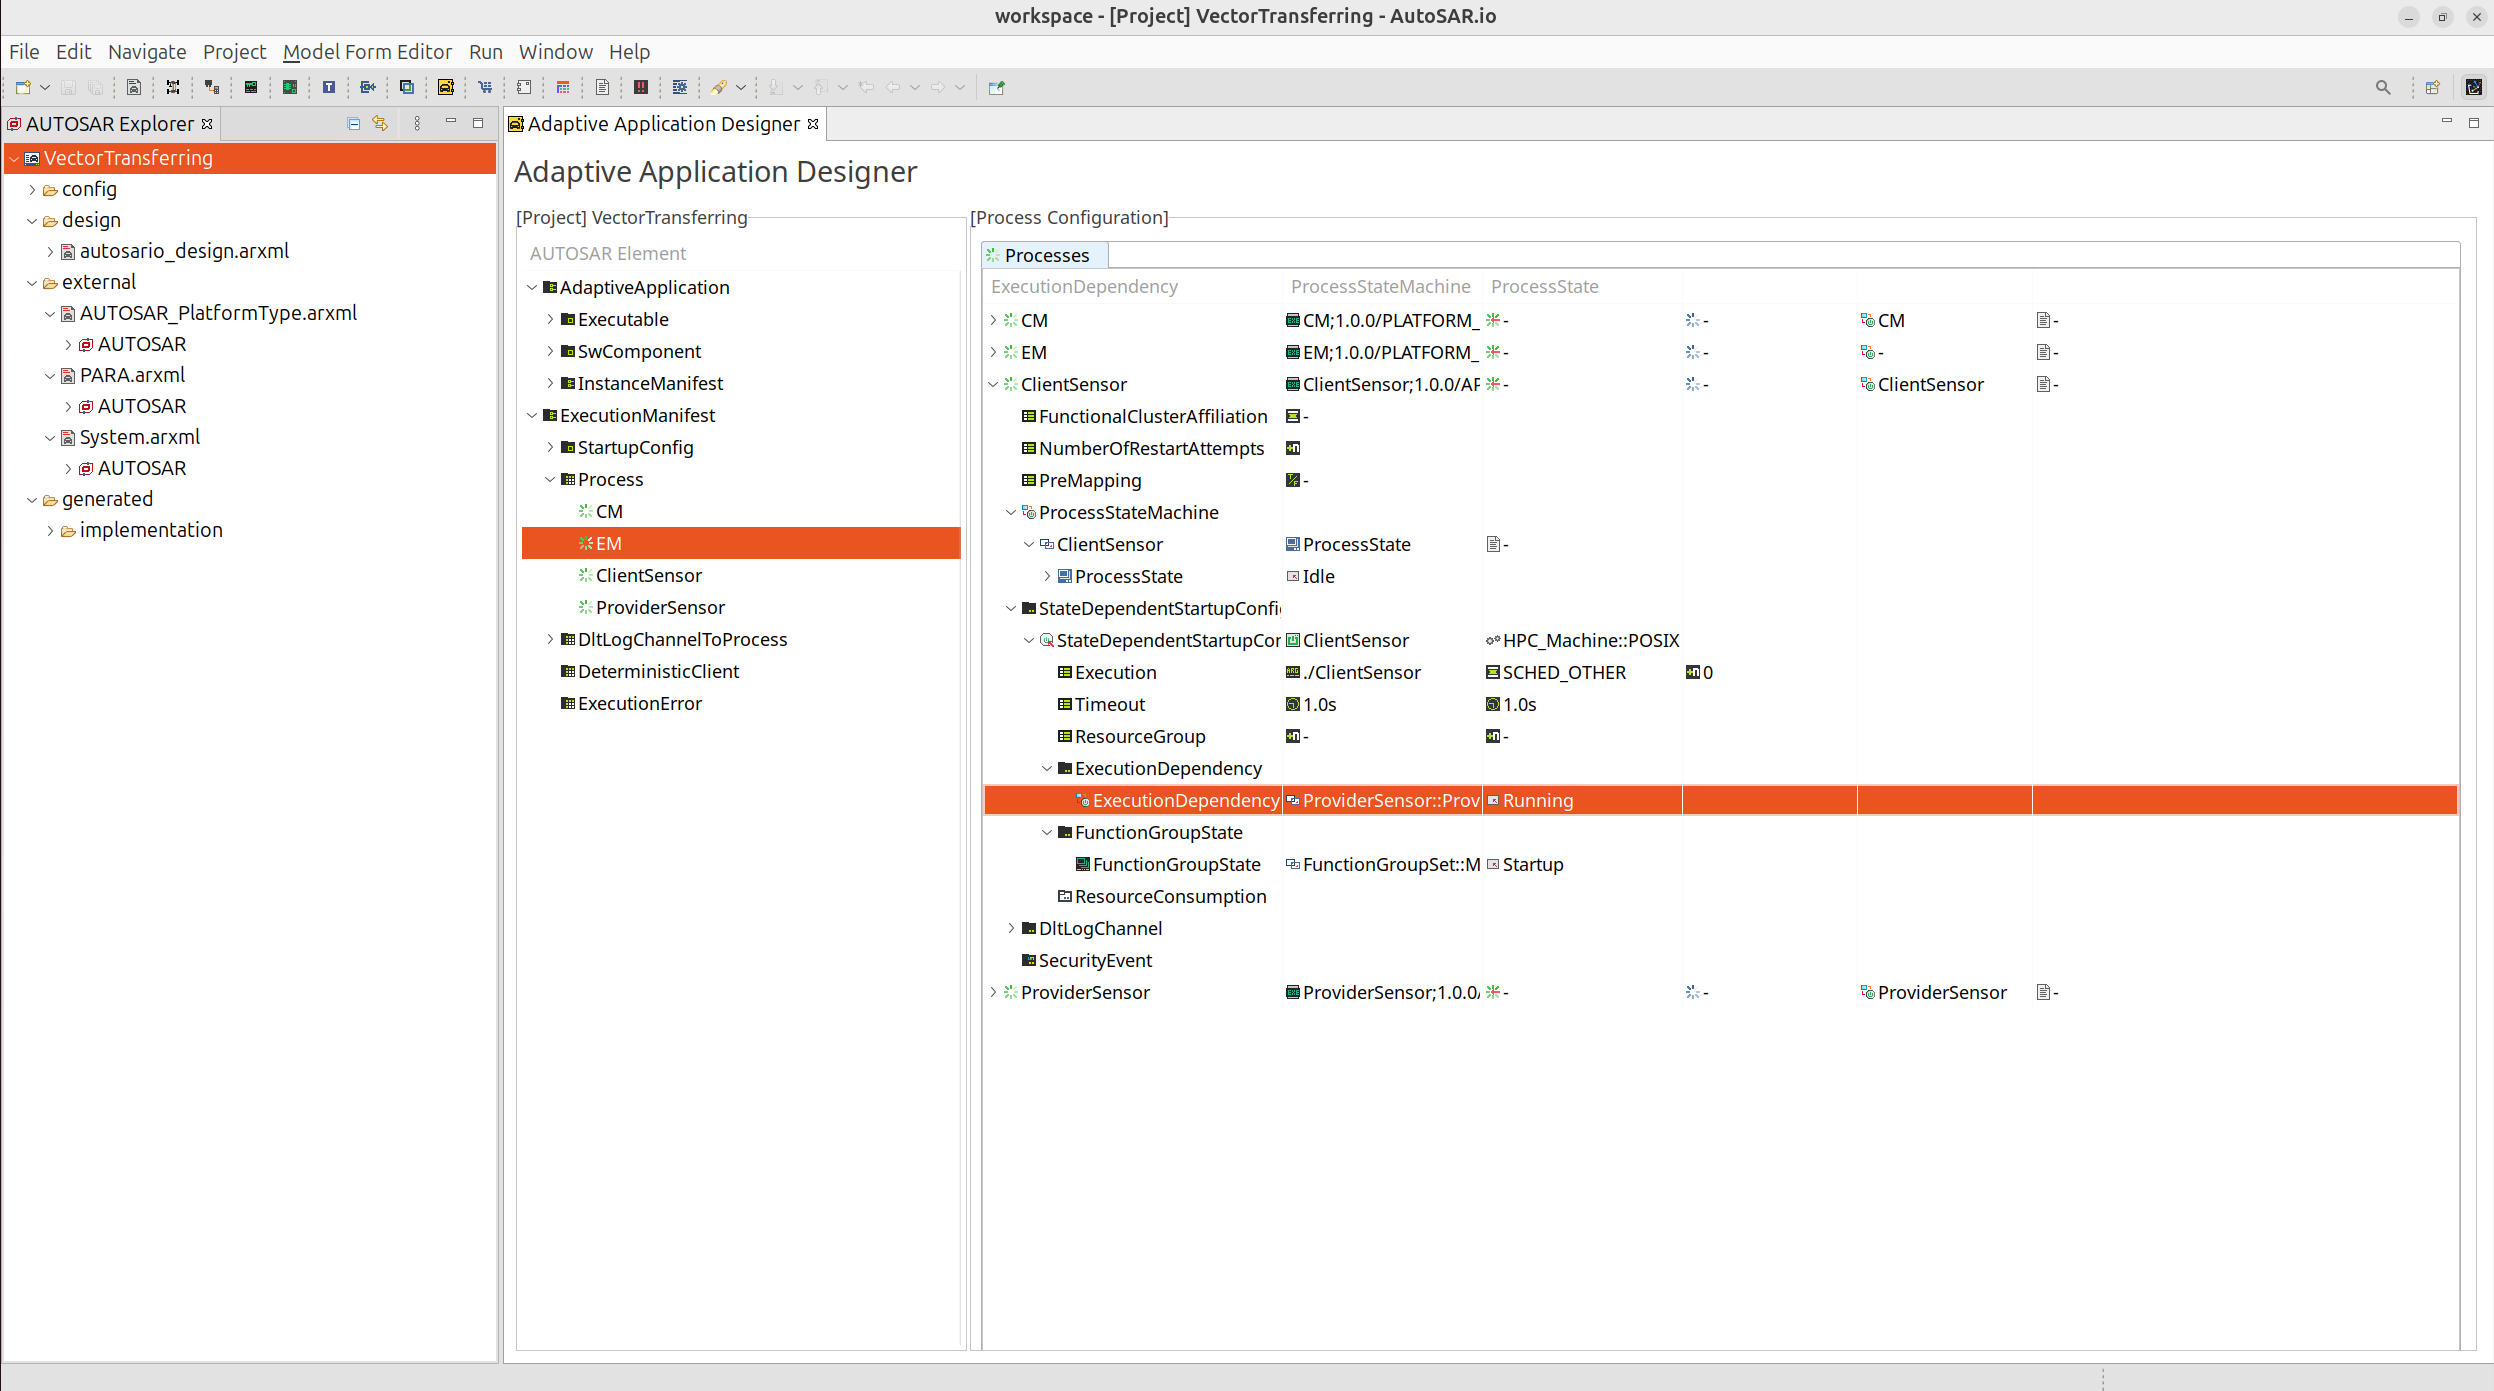
\includegraphics[width=0.75\textwidth]{Images/chap3/image_methodology/applicationDesign/configureClientProcess.png}
    \vspace{0.5cm}
    \caption{Configuration of Client Application Process}
    \label{fig:app_client_process_configuration}
\end{figure}

Figure~\ref{fig:app_client_process_configuration} shows a similar setup for the client application, where the \texttt{ClientSensor} executable is bound to its own process instance. Here, execution states and startup dependencies are defined to ensure that the client is activated only when required conditions are satisfied. This separation at the process level improves modularity and allows independent management of client and provider lifecycles.

% Map Application Processes to Target Machine
\begin{figure}[H]
    \centering
    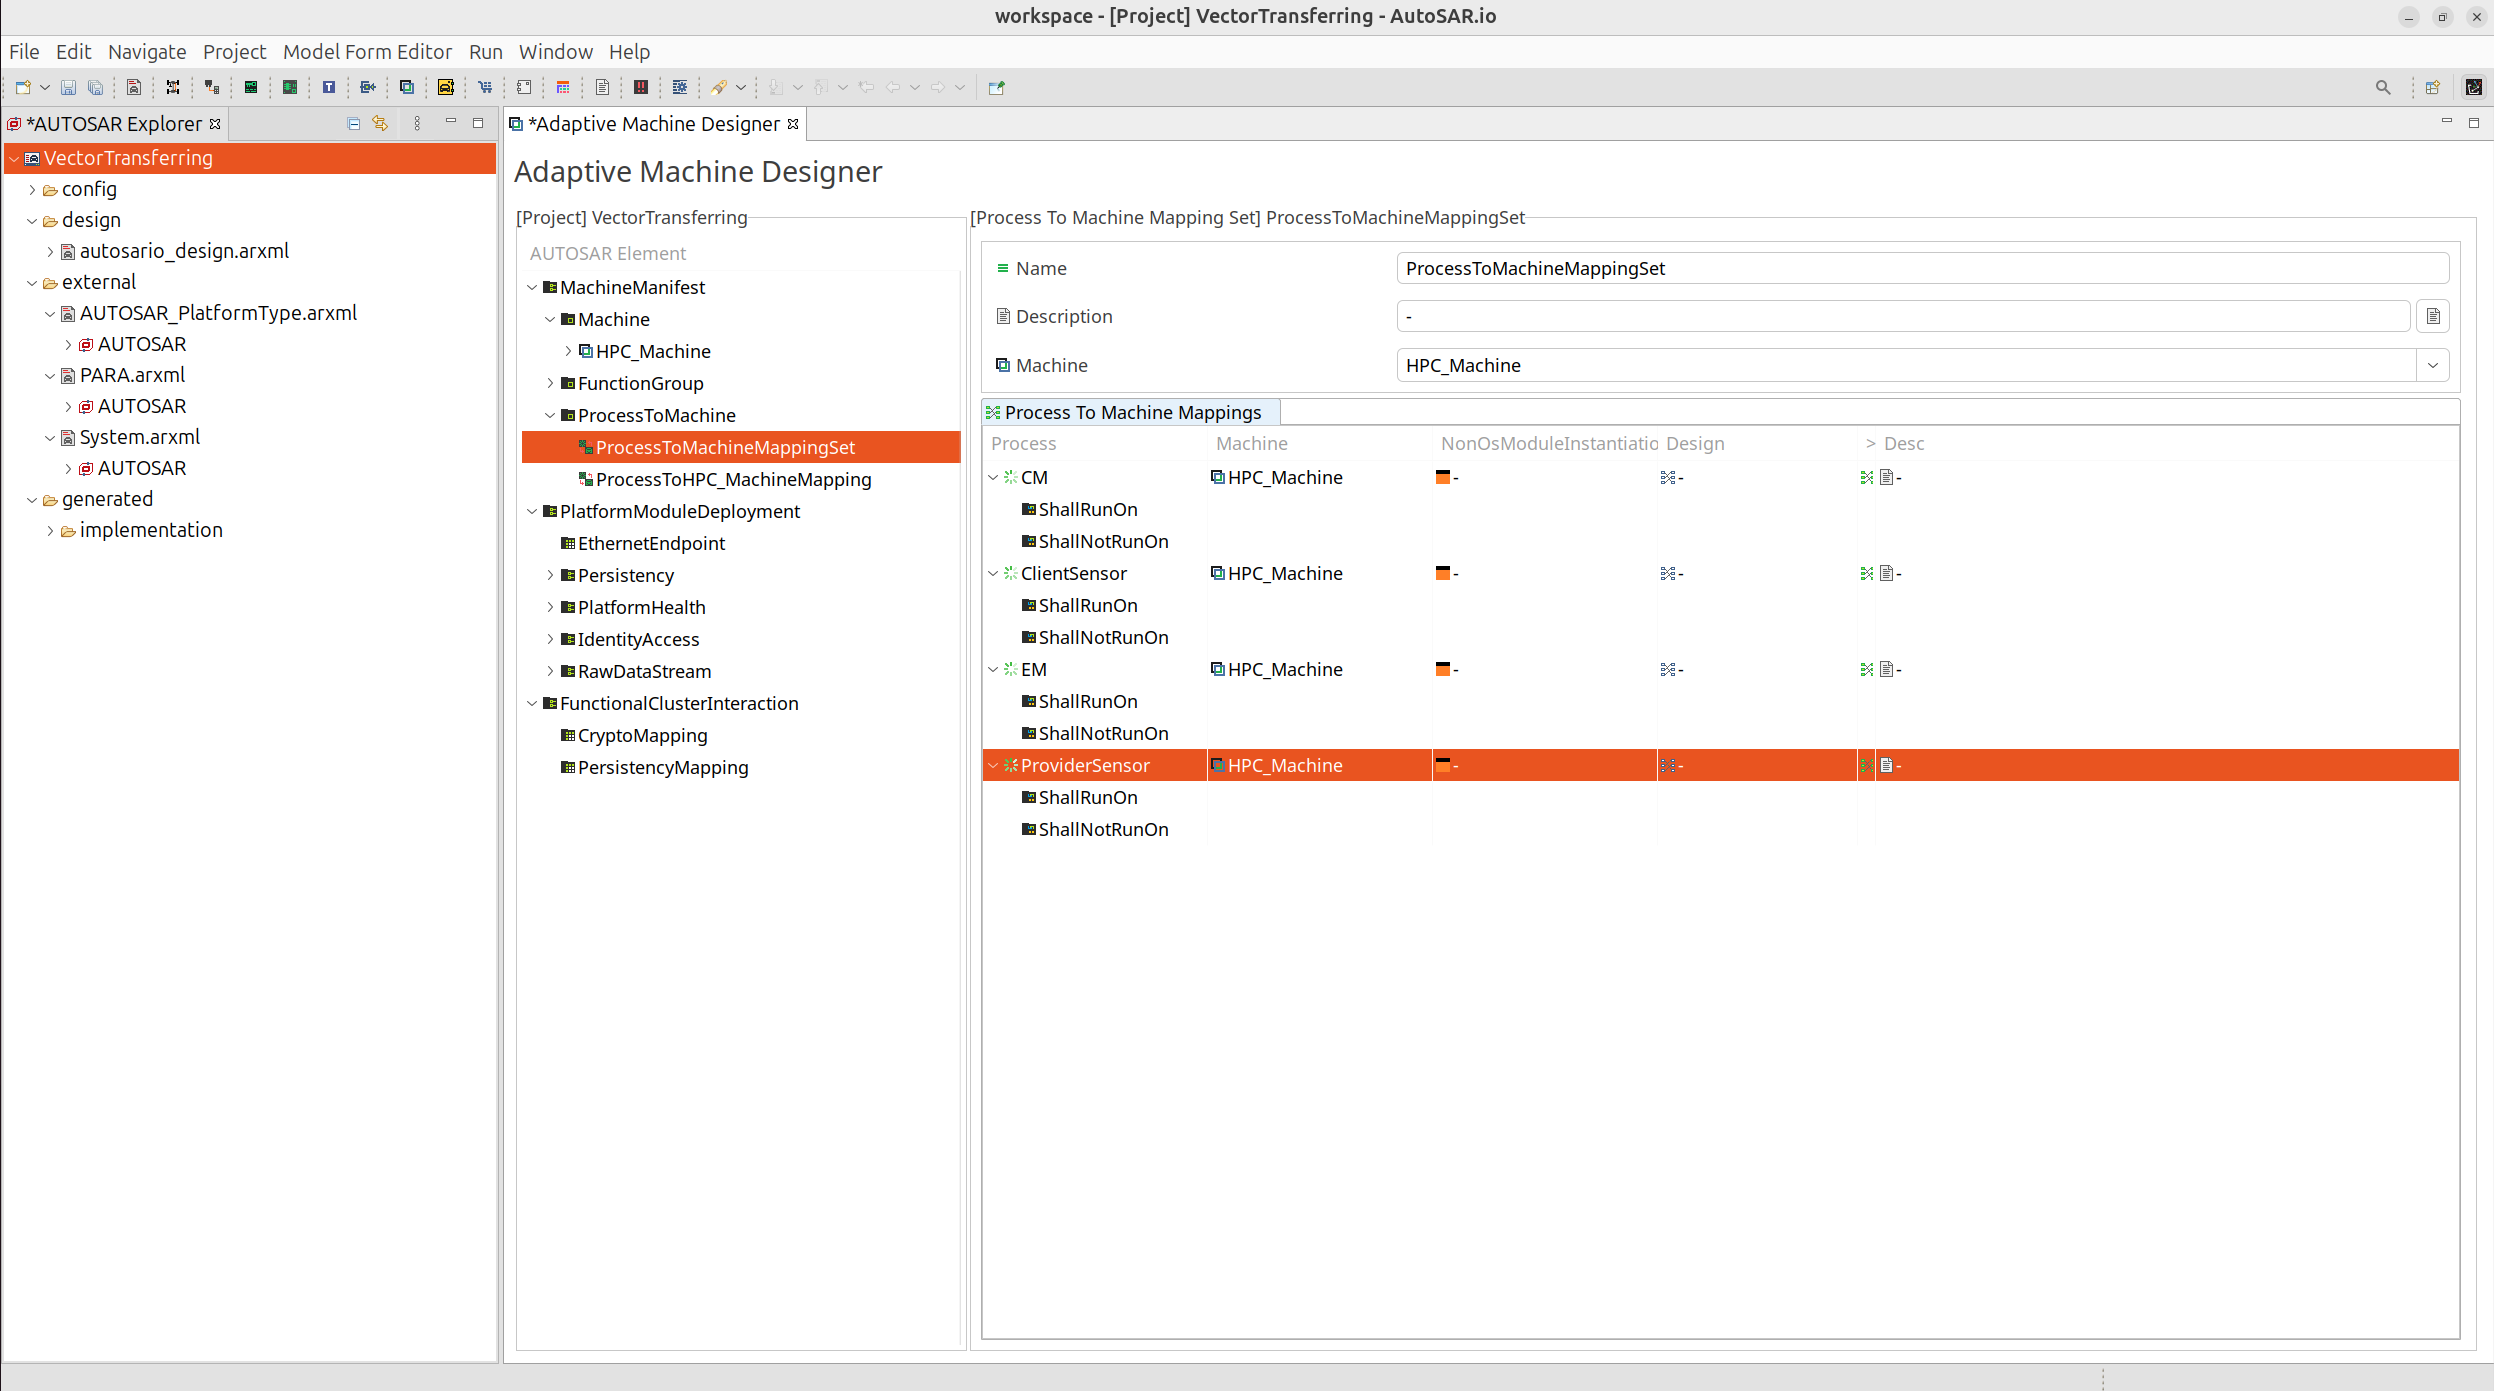
\includegraphics[width=0.75\textwidth]{Images/chap3/image_methodology/applicationDesign/mappingProcesstoMachine.png}
    \vspace{0.5cm}
    \caption{Mapping Application Processes to Target Machine}
    \label{fig:app_process_machine_mapping}
\end{figure}

Finally, Figure~\ref{fig:app_process_machine_mapping} presents the process-to-machine mapping defined in the Adaptive Machine Designer. In this step, all application processes, including \texttt{CM}, \texttt{EM}, \texttt{ClientSensor}, and \texttt{ProviderSensor}, are explicitly assigned to the target \texttt{HPC\_Machine}. This mapping determines the physical execution location of each process and establishes the final deployment relationship between the adaptive applications and the underlying hardware platform.

By consolidating all processes onto a single machine, the configuration ensures a coherent execution environment and simplifies resource management during runtime. This step completes the application deployment workflow by bridging the gap between application-level process definitions and machine-level execution, enabling the Adaptive AUTOSAR runtime to launch and supervise each process according to the previously defined startup, scheduling, and communication configurations.

\subsubsection{Generating Code and Manifest Files}
After completing the configuration steps at the machine, service, and application levels, the Autosar.io tool supports automatic generation of implementation artifacts through the PARA Generator. This generator collects all previously defined models, including Machine Manifests, service definitions, service instances, and application processes, and transforms them into deployable outputs that conform to the Adaptive AUTOSAR specification. By doing so, the tool ensures that the system configuration remains consistent from design time to implementation.

\begin{figure}[H]
    \centering
    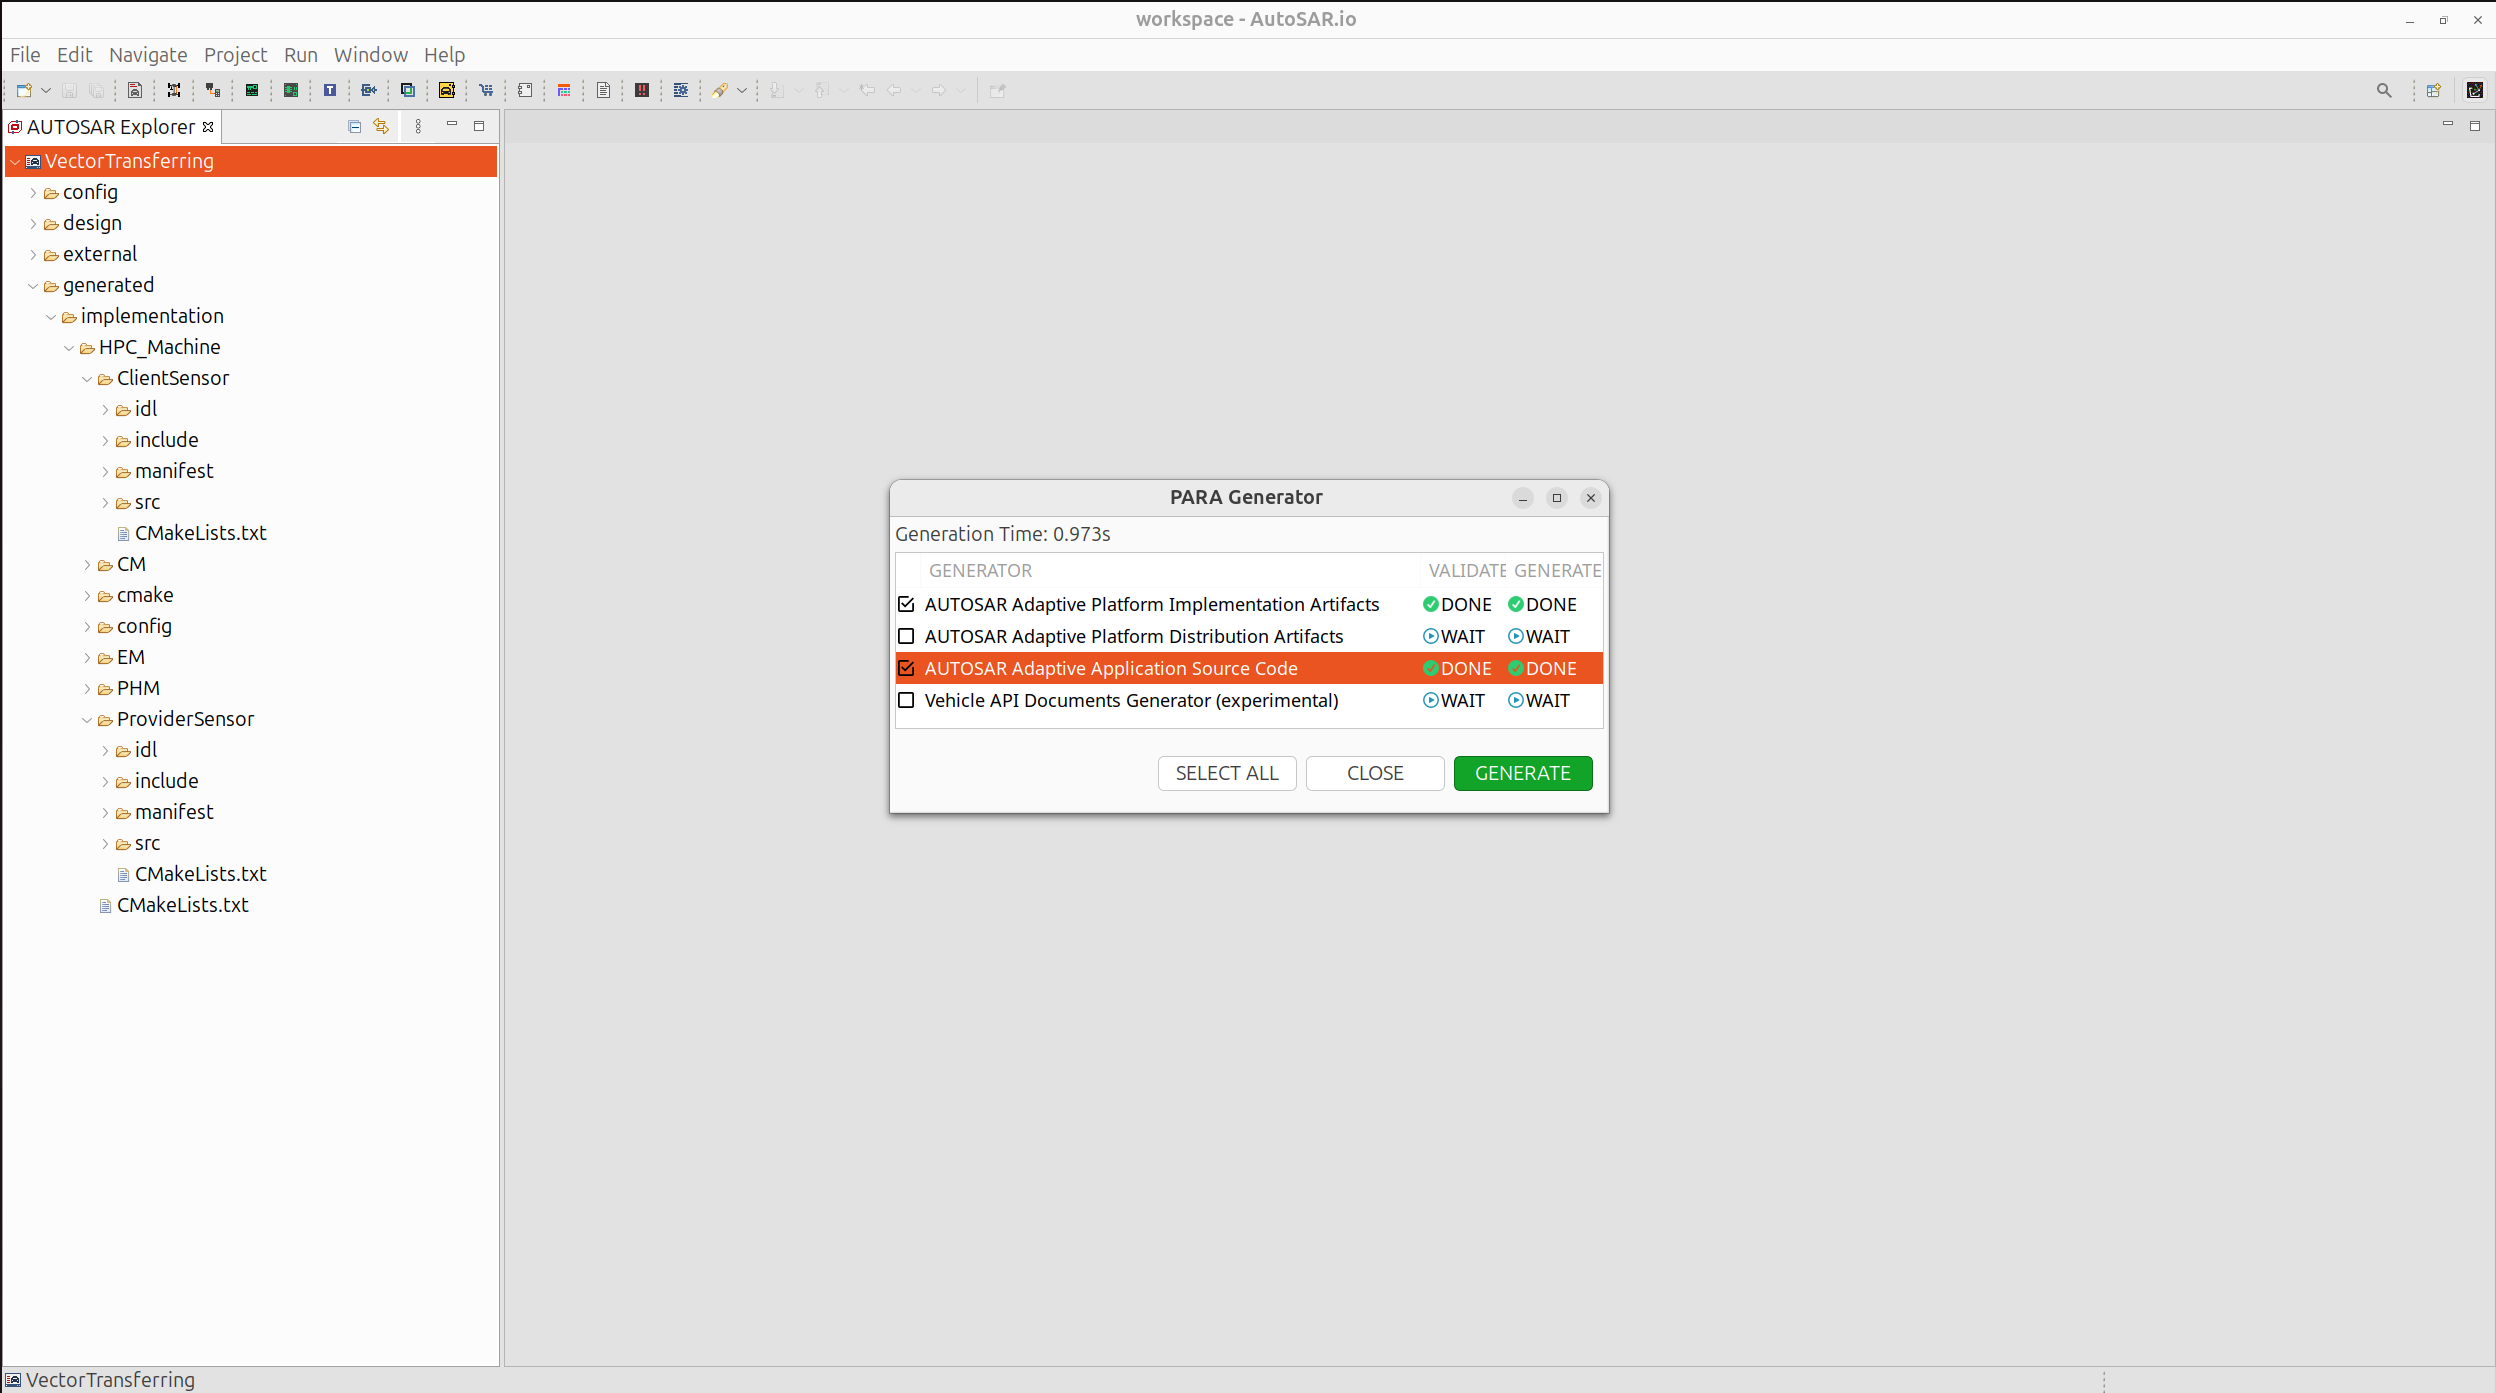
\includegraphics[width=0.75\textwidth]{Images/chap3/generating.png}
    \vspace{0.5cm}
    \caption{Generating Code and ARXML Files}
    \label{fig:code_generation}
\end{figure}

As illustrated in Figure~\ref{fig:code_generation}, the PARA Generator allows users to selectively generate different categories of artifacts, such as Adaptive Application source code, platform configuration files, and manifest descriptions. The generation process produces AUTOSAR compliant ARXML files together with structured C++ source code for each executable. These outputs follow a standardized directory layout, which simplifies subsequent build and integration steps.

Through this automated generation mechanism, Autosar.io bridges the gap between high level system modeling and concrete software artifacts. The generated code and configuration files serve as a reliable foundation for compilation, deployment, and runtime execution. This approach reduces manual errors, improves traceability, and supports a smooth transition from configuration to system integration in the Adaptive AUTOSAR development workflow.


Once the AUTOSAR platform configuration is established, a perception mechanism is required to detect traffic lights in real time. Consequently, the focus shifts to designing and training the YOLO-MobileNetV4 architecture, demonstrating how the core software platform integrates with edge-oriented AI components.

% In this work, we adopt a customized version of the YOLO detection framework by integrating the MobileNetV4 backbone in order to obtain a lightweight yet effective object detection model. The primary motivation behind this design choice is to reduce computational complexity and memory consumption while maintaining reliable detection accuracy. Such requirements are essential for deployment on resource constrained edge devices, including embedded systems, single board computers, and mobile platforms.

% MobileNetV4 is a recently proposed convolutional neural network architecture designed for universal deployment across mobile and edge hardware. It emphasizes efficient feature extraction through improved depthwise separable convolutions, universal inverted bottleneck blocks, and optimized layer scaling strategies. Compared to conventional backbones such as CSPDarknet or standard ResNet variants, MobileNetV4 provides a more balanced trade off between inference speed and representational capability. As a result, it is particularly suitable for real time computer vision tasks where latency, power consumption, and memory footprint are critical constraints.

% \subsection{Backbone Replacement Strategy}

% To integrate MobileNetV4 into the YOLO framework, the default backbone definition is replaced by a customized model configuration file, denoted as \texttt{yolo11-mobilenetv4.yaml}. This configuration follows the standard Ultralytics YOLO model definition format while modifying the backbone section to incorporate MobileNetV4 building blocks. The neck and detection head structures remain largely unchanged in order to preserve compatibility with existing loss functions, anchor settings, and training pipelines.

% The backbone replacement process is performed at the model configuration and module registration level rather than modifying the core training logic. This design choice improves maintainability and simplifies future updates of the YOLO framework. The integration procedure follows a publicly available technical guide that details how MobileNetV4 modules are registered, parsed, and treated as backbone components during model construction\footnote{Guideline for integrating MobileNetV4 into YOLO architectures is available at \url{https://blog.csdn.net/qq_44231797/article/details/147483132}.}. By preserving the feature pyramid structure, multi scale detection capability is maintained despite the lightweight backbone.

% \subsection{Model Initialization and Pretrained Weights}

% To accelerate convergence and improve training stability, the model is initialized using pretrained weights from a lightweight YOLO variant. Specifically, the \texttt{yolo11n.pt} checkpoint is loaded as the initial parameter set. Although the backbone architecture differs from the original YOLO design, partial weight transfer remains beneficial for shared components such as the detection head and certain convolutional layers.

% The Ultralytics YOLO API automatically performs parameter matching where possible and ignores incompatible layers. This mechanism enables the model to leverage prior knowledge while avoiding structural conflicts during initialization. As a result, the training process converges more reliably compared to training from scratch.

% \subsection{Training Configuration}

% The training process is conducted using the Ultralytics YOLO training interface, which provides a flexible and reproducible pipeline for object detection tasks. Dataset information is specified through a YAML configuration file that defines training and validation paths, class labels, and metadata. All input images are resized to a resolution of $320 \times 320$ pixels in order to balance detection accuracy and computational efficiency.

% Stochastic Gradient Descent is selected as the optimization algorithm due to its stable convergence behavior for large scale detection models. Automatic mixed precision is enabled to reduce GPU memory usage and accelerate training while maintaining numerical stability. The model is trained for a total of 400 epochs to ensure sufficient convergence given the modified backbone structure.

% \subsection{Training Script}

% The complete training script used in this study is shown below. This script defines the model configuration, loads pretrained weights, and executes the training process with the selected hyperparameters.

% \begin{lstlisting}[language=Python, caption={YOLO-MobileNetV4 Training Script}]
% # Model configuration file
% model_yaml_path = r"yolo11-mobilenetv4.yaml"

% # Dataset configuration file
% data_yaml_path = r"dataset/data.yaml"

% # Pretrained model
% pre_model_name = "yolo11n.pt"

% import warnings
% warnings.filterwarnings("ignore")

% from ultralytics import YOLO

% if __name__ == "__main__":
%     model = YOLO(model_yaml_path)
%     model.load(pre_model_name)

%     model.train(
%         data=data_yaml_path,
%         cache=False,
%         imgsz=320,
%         epochs=400,
%         workers=8,
%         device="0",
%         optimizer="SGD",
%         amp=True,
%         project="runs/train-yolo-mobilenetv4",
%         name="exp"
%     )
% \end{lstlisting}

\section{YOLO-MobileNetV4 Model}

In this work, we adopt a customized version of the YOLOv26 detection framework by integrating the MobileNetV4 backbone in order to obtain a lightweight yet effective object detection model. The primary motivation behind this design choice is to reduce computational complexity and memory consumption while maintaining reliable detection accuracy. Such requirements are essential for deployment on resource constrained edge devices, including embedded systems, single board computers, and mobile platforms.

\subsection{Integrating MobileNetv4 into YOLO}

Following the our paper in \hyperref[chap:append]{Appendix}, we will continue to integrate MobileNetV4 as the feature extractor for YOLO26 creates a hybrid "YOLO-MNv4" architecture that is theoretically optimal for autonomous driving. On mobile accelerators like the Pixel EdgeTPU, MNv4 is approximately twice as fast as MobileNetV3 for equivalent accuracy due to its high operational intensity. Replacing the standard YOLO26 backbone with MNv4 significantly reduces the floating-point operations (FLOPs) required per inference. This architecture specifically excels in occlusion handling, where the advanced receptive fields of the UIB blocks allow the model to infer the presence of a traffic light even when it is partially obscured by large vehicles, ensuring a robust and reliable perception system.

To adapt the original YOLO26 architecture for edge deployment, several crucial modifications were made (comparing Figure \ref{fig:yolo26_original_arch} to Figure \ref{fig:yolo26_mnv4_arch}). First, the standard heavy CNN backbone was replaced entirely with {MobileNetV4ConvSmall050}. Second, the original 4-head Feature Pyramid Network (P2, P3, P4, P5) was scaled down to a {3-head architecture} (P3, P4, P5) by removing the high-resolution P2 feature extraction path and its corresponding detection head. This reduction dramatically lowers the computational complexity (GFLOPs) and parameter count. Meanwhile, the advanced components of the YOLO26 neck—including the {C3k2} fusion blocks, {SPPF}, {C2PSA} spatial attention, and the {One-to-One Head}-were preserved to maintain state-of-the-art detection logic.

\begin{figure}[htbp]
    \centering
    \resizebox{\textwidth}{!}{
    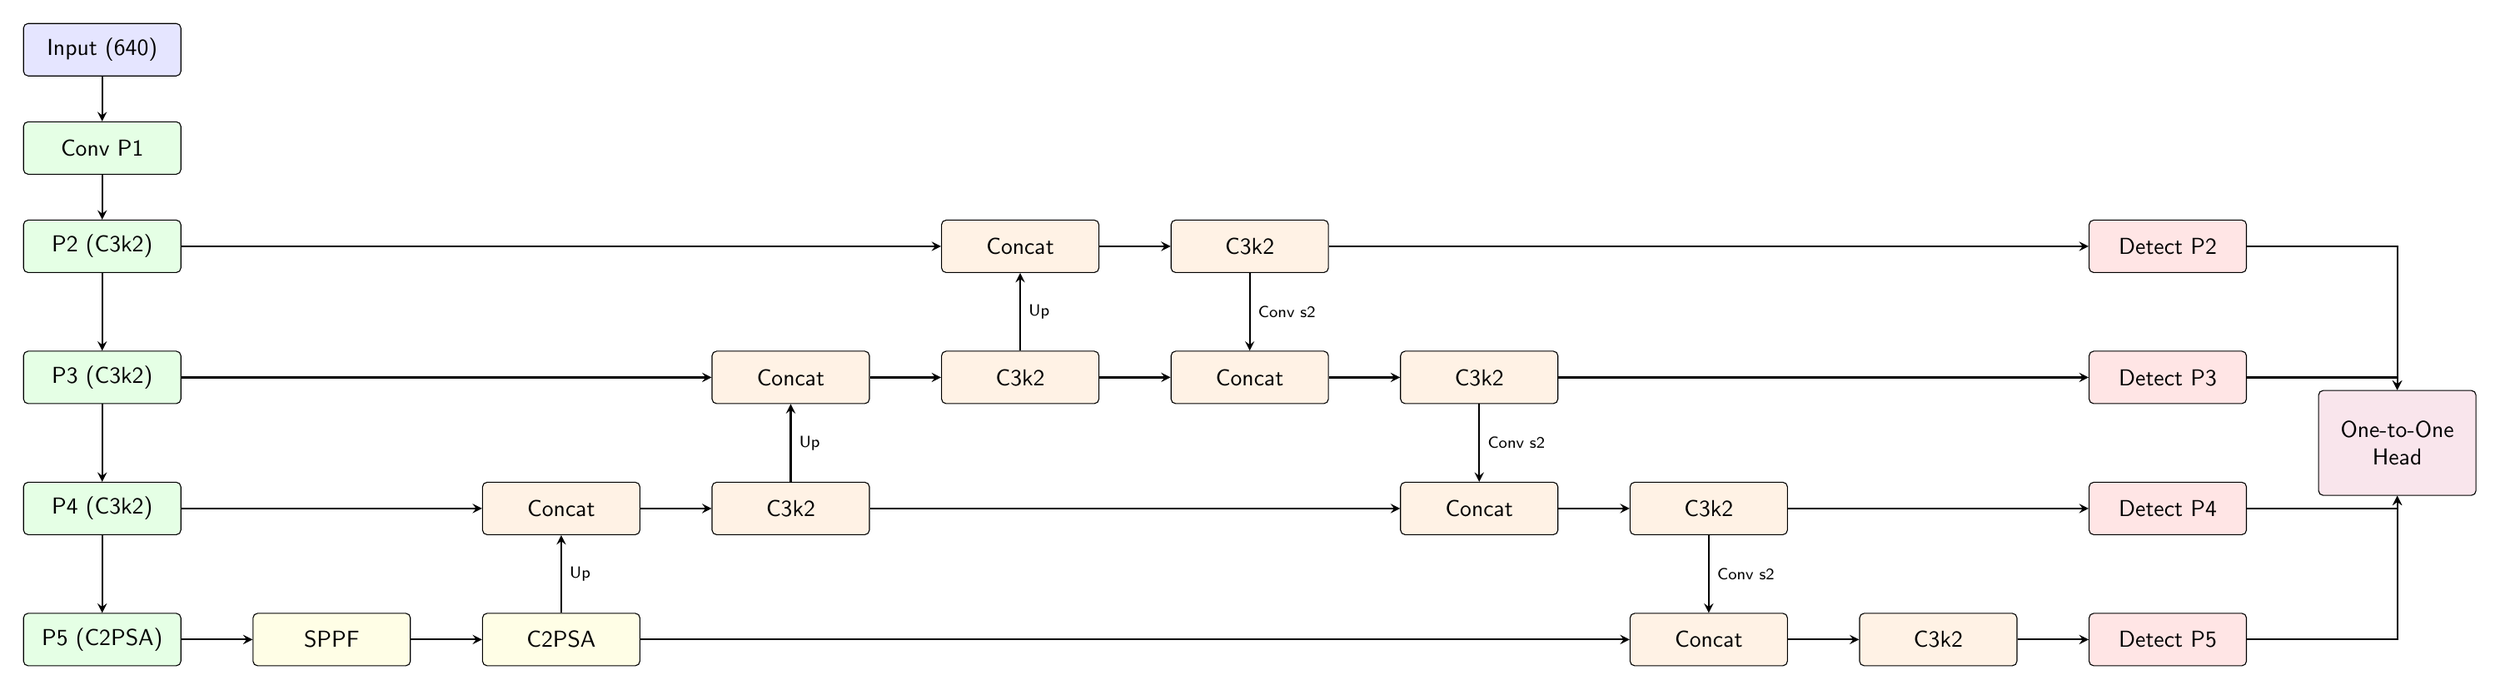
\begin{tikzpicture}[
        box/.style={rectangle, draw, minimum width=2.4cm, minimum height=0.8cm, text centered, font=\sffamily, rounded corners=2pt},
        arrow/.style={->, >=stealth, thick},
        label/.style={font=\sffamily\scriptsize}
    ]

    % Backbone
    \node[box, fill=blue!10] (input) at (0, 9) {Input (640)};
    \node[box, fill=green!10] (conv1) at (0, 7.5) {Conv P1};
    \node[box, fill=green!10] (p2) at (0, 6) {P2 (C3k2)};
    \node[box, fill=green!10] (p3) at (0, 4) {P3 (C3k2)};
    \node[box, fill=green!10] (p4) at (0, 2) {P4 (C3k2)};
    \node[box, fill=green!10] (p5) at (0, 0) {P5 (C2PSA)};

    \draw[arrow] (input) -- (conv1);
    \draw[arrow] (conv1) -- (p2);
    \draw[arrow] (p2) -- (p3);
    \draw[arrow] (p3) -- (p4);
    \draw[arrow] (p4) -- (p5);

    % SPPF & C2PSA
    \node[box, fill=yellow!10] (sppf) at (3.5, 0) {SPPF};
    \node[box, fill=yellow!10] (c2psa) at (7.0, 0) {C2PSA};
    \draw[arrow] (p5) -- (sppf);
    \draw[arrow] (sppf) -- (c2psa);

    % Neck - Top-down
    \node[box, fill=orange!10] (cat_p4) at (7.0, 2) {Concat};
    \node[box, fill=orange!10] (c3k2_td_p4) at (10.5, 2) {C3k2};
    \draw[arrow] (c2psa) -- node[right, label] {Up} (cat_p4);
    \draw[arrow] (p4) -- (cat_p4);
    \draw[arrow] (cat_p4) -- (c3k2_td_p4);

    \node[box, fill=orange!10] (cat_p3) at (10.5, 4) {Concat};
    \node[box, fill=orange!10] (c3k2_td_p3) at (14.0, 4) {C3k2};
    \draw[arrow] (c3k2_td_p4) -- node[right, label] {Up} (cat_p3);
    \draw[arrow] (p3) -- (cat_p3);
    \draw[arrow] (cat_p3) -- (c3k2_td_p3);

    \node[box, fill=orange!10] (cat_p2) at (14.0, 6) {Concat};
    \node[box, fill=orange!10] (c3k2_td_p2) at (17.5, 6) {C3k2};
    \draw[arrow] (c3k2_td_p3) -- node[right, label] {Up} (cat_p2);
    \draw[arrow] (p2) -- (cat_p2);
    \draw[arrow] (cat_p2) -- (c3k2_td_p2);

    % Neck - Bottom-up
    \node[box, fill=orange!10] (cat_p3_bu) at (17.5, 4) {Concat};
    \node[box, fill=orange!10] (c3k2_bu_p3) at (21.0, 4) {C3k2};
    \draw[arrow] (c3k2_td_p2) -- node[right, label] {Conv s2} (cat_p3_bu);
    \draw[arrow] (c3k2_td_p3) -- (cat_p3_bu);
    \draw[arrow] (cat_p3_bu) -- (c3k2_bu_p3);

    \node[box, fill=orange!10] (cat_p4_bu) at (21.0, 2) {Concat};
    \node[box, fill=orange!10] (c3k2_bu_p4) at (24.5, 2) {C3k2};
    \draw[arrow] (c3k2_bu_p3) -- node[right, label] {Conv s2} (cat_p4_bu);
    \draw[arrow] (c3k2_td_p4) -- (cat_p4_bu);
    \draw[arrow] (cat_p4_bu) -- (c3k2_bu_p4);

    \node[box, fill=orange!10] (cat_p5_bu) at (24.5, 0) {Concat};
    \node[box, fill=orange!10] (c3k2_bu_p5) at (28.0, 0) {C3k2};
    \draw[arrow] (c3k2_bu_p4) -- node[right, label] {Conv s2} (cat_p5_bu);
    \draw[arrow] (c2psa) -- (cat_p5_bu);
    \draw[arrow] (cat_p5_bu) -- (c3k2_bu_p5);

    % Detectors
    \node[box, fill=red!10] (head2) at (31.5, 6) {Detect P2};
    \node[box, fill=red!10] (head3) at (31.5, 4) {Detect P3};
    \node[box, fill=red!10] (head4) at (31.5, 2) {Detect P4};
    \node[box, fill=red!10] (head5) at (31.5, 0) {Detect P5};
    
    \node[box, fill=purple!10, align=center, minimum height=1.6cm] (detect) at (35.0, 3) {One-to-One\\Head};

    \draw[arrow] (c3k2_td_p2) -- (head2);
    \draw[arrow] (c3k2_bu_p3) -- (head3);
    \draw[arrow] (c3k2_bu_p4) -- (head4);
    \draw[arrow] (c3k2_bu_p5) -- (head5);
    
    \draw[arrow] (head2) -| (detect);
    \draw[arrow] (head3) -| (detect);
    \draw[arrow] (head4) -| (detect);
    \draw[arrow] (head5) -| (detect);

    \end{tikzpicture}
    }
    \vspace{0.5cm}
    \caption{Architecture of the original YOLO26-p2 model with 4-head detection mechanism (P2/P3/P4/P5 outputs) for standard object detection tasks. Channel widths scale with the chosen model variant (n/s/m/l/x).}
    \label{fig:yolo26_original_arch}
\end{figure}

\begin{figure}[htbp]
    \centering
    \resizebox{\textwidth}{!}{
    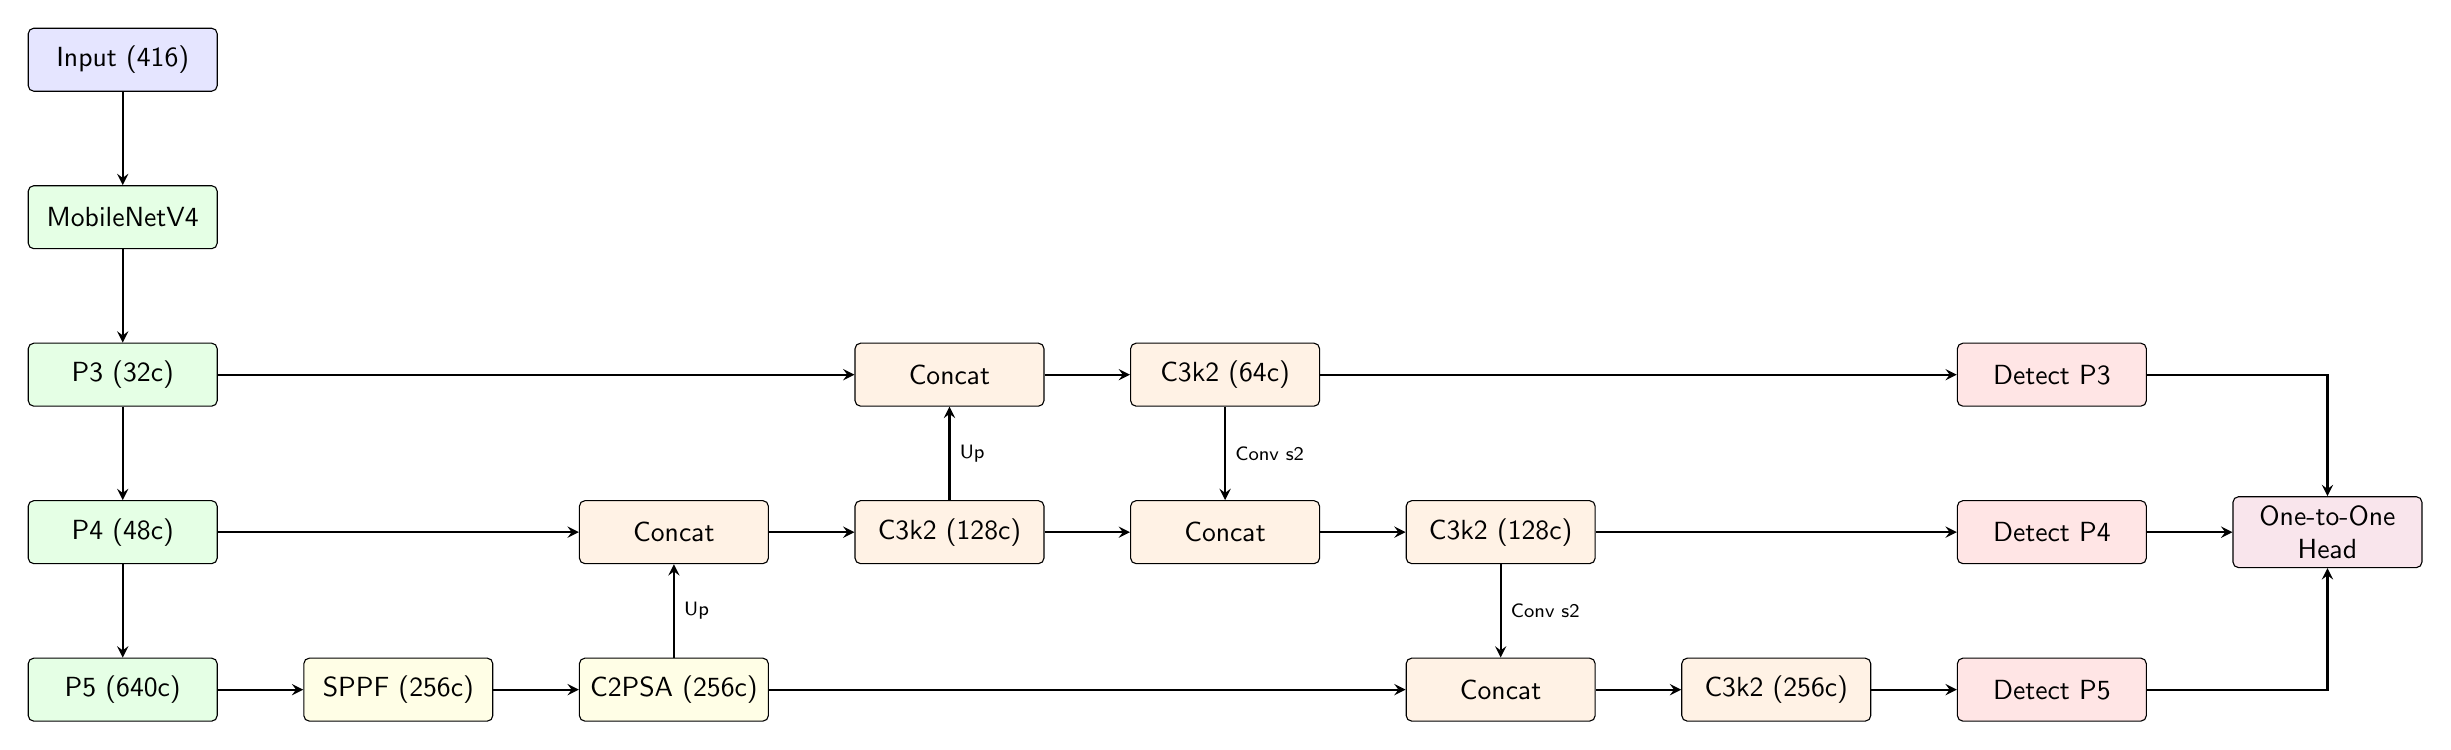
\begin{tikzpicture}[
        box/.style={rectangle, draw, minimum width=2.4cm, minimum height=0.8cm, text centered, font=\sffamily, rounded corners=2pt},
        arrow/.style={->, >=stealth, thick},
        label/.style={font=\sffamily\scriptsize}
    ]

    % X coordinates:
    % 0.0: Backbone
    % 3.5: SPPF
    % 7.0: C2PSA, cat1
    % 10.5: c3k2_1, cat2
    % 14.0: c3k2_2, cat3
    % 17.5: c3k2_3, cat4
    % 21.0: c3k2_4
    % 24.5: Detectors
    % 28.0: Head

    % Backbone
    \node[box, fill=blue!10] (input) at (0, 8) {Input (416)};
    \node[box, fill=green!10] (mnv4) at (0, 6) {MobileNetV4};
    \node[box, fill=green!10] (p3) at (0, 4) {P3 (32c)};
    \node[box, fill=green!10] (p4) at (0, 2) {P4 (48c)};
    \node[box, fill=green!10] (p5) at (0, 0) {P5 (640c)};

    \draw[arrow] (input) -- (mnv4);
    \draw[arrow] (mnv4) -- (p3);
    \draw[arrow] (p3) -- (p4);
    \draw[arrow] (p4) -- (p5);

    % SPPF & C2PSA
    \node[box, fill=yellow!10] (sppf) at (3.5, 0) {SPPF (256c)};
    \node[box, fill=yellow!10] (c2psa) at (7.0, 0) {C2PSA (256c)};
    \draw[arrow] (p5) -- (sppf);
    \draw[arrow] (sppf) -- (c2psa);

    % Neck - Top-down
    \node[box, fill=orange!10] (cat1) at (7.0, 2) {Concat};
    \node[box, fill=orange!10] (c3k2_1) at (10.5, 2) {C3k2 (128c)};
    \draw[arrow] (c2psa) -- node[right, label] {Up} (cat1);
    \draw[arrow] (p4) -- (cat1);
    \draw[arrow] (cat1) -- (c3k2_1);

    \node[box, fill=orange!10] (cat2) at (10.5, 4) {Concat};
    \node[box, fill=orange!10] (c3k2_2) at (14.0, 4) {C3k2 (64c)};
    \draw[arrow] (c3k2_1) -- node[right, label] {Up} (cat2);
    \draw[arrow] (p3) -- (cat2);
    \draw[arrow] (cat2) -- (c3k2_2);

    % Neck - Bottom-up
    \node[box, fill=orange!10] (cat3) at (14.0, 2) {Concat};
    \node[box, fill=orange!10] (c3k2_3) at (17.5, 2) {C3k2 (128c)};
    \draw[arrow] (c3k2_2) -- node[right, label] {Conv s2} (cat3);
    \draw[arrow] (c3k2_1) -- (cat3);
    \draw[arrow] (cat3) -- (c3k2_3);

    \node[box, fill=orange!10] (cat4) at (17.5, 0) {Concat};
    \node[box, fill=orange!10] (c3k2_4) at (21.0, 0) {C3k2 (256c)};
    \draw[arrow] (c3k2_3) -- node[right, label] {Conv s2} (cat4);
    \draw[arrow] (c2psa) -- (cat4);
    \draw[arrow] (cat4) -- (c3k2_4);

    % Detectors
    \node[box, fill=red!10] (head1) at (24.5, 4) {Detect P3};
    \node[box, fill=red!10] (head2) at (24.5, 2) {Detect P4};
    \node[box, fill=red!10] (head3) at (24.5, 0) {Detect P5};
    
    \node[box, fill=purple!10, align=center] (detect) at (28.0, 2) {One-to-One\\Head};

    \draw[arrow] (c3k2_2) -- (head1);
    \draw[arrow] (c3k2_3) -- (head2);
    \draw[arrow] (c3k2_4) -- (head3);
    
    \draw[arrow] (head1) -| (detect);
    \draw[arrow] (head2) -- (detect);
    \draw[arrow] (head3) -| (detect);

    \end{tikzpicture}
    }
    \vspace{0.5cm} % Add some space before caption to prevent overlap
    \caption{Architecture of the YOLO26 model with MobileNetV4ConvSmall050 backbone, dual-head mechanism, and NMS-free end-to-end detection, tailored for $416\times416$ resolution.}
    \label{fig:yolo26_mnv4_arch}
\end{figure}

% \subsection{Training Hyperparameters}

% The training process is conducted using the Ultralytics YOLO training API, which provides a reproducible and configurable pipeline for object detection tasks. The dataset is specified through a YAML configuration file (\texttt{TrafficLightV5.v9i.yolo26/data.yaml}) that defines training and validation image paths, class labels, and metadata. To bootstrap training, pretrained weights from \texttt{yolo26n.pt} are loaded via partial weight transfer; compatible layers (primarily in the neck and head) inherit learned parameters, while the MobileNetV4 backbone is initialised from scratch. The \texttt{end2end=True} flag activates the One-to-One head for NMS-free training. Table~\ref{tab:hyperparams} summarises the key hyperparameters.

% \begin{table}[htbp]
% \centering
% \caption{Selected training hyperparameters for the YOLO26-MobileNetV4 model.}
% \label{tab:hyperparams}
% \renewcommand{\arraystretch}{1.15}
% \begin{tabular}{l l l}
% \hline
% \textbf{Parameter} & \textbf{Value} & \textbf{Rationale} \\
% \hline
% \texttt{imgsz} & $416 \times 416$ & Balance between spatial resolution and edge inference speed \\
% \texttt{epochs} & 100 & Sufficient convergence for the modified backbone \\
% \texttt{batch} & 16 & Fits within GPU memory with MobileNetV4 backbone \\
% \texttt{patience} & 100 & Disable early stopping; run full cosine LR cycle \\
% \texttt{optimizer} & auto (SGD) & Stable convergence for detection models \\
% \texttt{lr0} & 0.005 & Slightly elevated initial LR for unfrozen backbone \\
% \texttt{lrf} & 0.01 & Final LR ratio: $\text{lr}_{\text{final}} = 0.01 \times \text{lr}_0$ \\
% \texttt{cos\_lr} & True & Cosine annealing for smooth convergence in late epochs \\
% \texttt{warmup\_epochs} & 3.0 & Gradual LR ramp-up to stabilise early gradients \\
% \texttt{amp} & True & Mixed-precision training for memory efficiency \\
% \texttt{freeze} & None & All layers trainable; no backbone freezing \\
% \texttt{close\_mosaic} & 10 & Disable mosaic augmentation in the last 10 epochs \\
% \hline
% \texttt{box} & 7.5 & Bounding box regression loss weight \\
% \texttt{cls} & 0.5 & Classification loss weight \\
% \texttt{dfl} & 1.5 & DFL loss weight (set but unused since YOLO26 removes DFL) \\
% \hline
% \end{tabular}
% \end{table}

% \subsubsection{Optimiser and Learning Rate Schedule}
% The optimiser is set to \texttt{auto}, which defaults to Stochastic Gradient Descent (SGD) with Nesterov momentum ($\mu = 0.937$) and weight decay ($\lambda = 5 \times 10^{-4}$). The initial learning rate is set to $\text{lr}_0 = 0.005$, slightly higher than the default $0.01$ to compensate for the unfrozen MobileNetV4 backbone requiring larger gradient steps to adapt to the traffic light domain. A cosine annealing schedule (\texttt{cos\_lr=True}) smoothly decays the learning rate to $\text{lr}_0 \times \text{lrf} = 5 \times 10^{-5}$ over the full 100 epochs, ensuring fine-grained convergence in the later stages of training without the abrupt transitions of step-decay schedules.

% \subsubsection{No Backbone Freezing}
% Unlike transfer learning approaches that freeze the backbone during initial epochs, this configuration leaves all layers trainable (\texttt{freeze=None}). Since the MobileNetV4ConvSmall050 backbone differs fundamentally from the original YOLO26 backbone, the pretrained weights only partially transfer. Freezing would prevent the new backbone from learning domain-specific features such as the distinctive shapes and colours of Vietnamese traffic light signal heads and arrow indicators.

% \subsubsection{Image Augmentation Strategy}
% The augmentation pipeline is carefully tuned for the traffic light detection domain:

% \begin{itemize}
%     \item \textbf{Colour jitter}: Hue shift is minimal (\texttt{hsv\_h}$=0.015$) to preserve the critical red/green/yellow colour semantics of traffic signals. Saturation (\texttt{hsv\_s}$=0.7$) and brightness (\texttt{hsv\_v}$=0.4$) augmentation are moderate to improve robustness under varying lighting conditions without corrupting colour-dependent class distinctions.
%     \item \textbf{Geometric transforms}: Translation (\texttt{translate}$=0.1$) and scale (\texttt{scale}$=0.5$) are enabled to simulate varying camera distances and positions. Rotation (\texttt{degrees}$=0.0$) and shear (\texttt{shear}$=0.0$) are disabled since traffic lights are always vertically oriented.
%     \item \textbf{Flipping disabled}: Both horizontal (\texttt{fliplr}$=0.0$) and vertical (\texttt{flipud}$=0.0$) flips are strictly disabled. Horizontal flipping would reverse the direction of left/right arrow turn signals, creating incorrect training labels.
%     \item \textbf{Mosaic}: Set to 0.5 probability to composite multiple training images into one frame, improving the model's ability to detect small, densely packed objects such as timer digit clusters. Mosaic is automatically disabled in the last 10 epochs (\texttt{close\_mosaic}$=10$) so the model fine-tunes on unmodified real images.
%     \item \textbf{MixUp and CopyPaste}: Both disabled (\texttt{mixup}$=0.0$, \texttt{copy\_paste}$=0.0$) to avoid blending signals from different classes, which could confuse the network on colour-critical traffic light states.
% \end{itemize}


\subsection{Dataset and Hyper parameters}
\label{sub:datasetYolo}
A well-prepared dataset and carefully tuned hyperparameters are essential for successfully training the modified YOLO-MobileNetV4 model. This section details the dataset used for traffic light detection, including its composition and pre-processing steps, before explaining the specific training configurations and augmentation strategies applied to ensure robust performance.

\subsubsection{Dataset Composition and Pre-processing}
The model is trained and evaluated on the \texttt{TrafficLightV5.v9i.yolo26} dataset, which comprises a total of 4,867 images. The dataset is annotated in the YOLO format and structured to detect four classes: \texttt{left}, \texttt{right}, \texttt{straight}, and \texttt{timer}. The images are partitioned into three splits: 4,260 images for training, 406 for validation, and 201 for testing. Prior to model ingestion, offline pre-processing and augmentations were applied via Roboflow. The pre-processing includes auto-orientation and resizing to $416 \times 416$ pixels (fit with black edges). The offline augmentation strategy generates three versions of each source image by applying random rotation ($-5^\circ$ to $+5^\circ$), random shear ($-2^\circ$ to $+2^\circ$), exposure adjustments ($\pm 10\%$), and salt-and-pepper noise ($0.1\%$ of pixels).

\subsubsection{Training Configuration}
The training process is conducted using the Ultralytics YOLO training API, which provides a reproducible and configurable pipeline for object detection tasks. The dataset is specified through a YAML configuration file (\texttt{TrafficLightV5.v9i.yolo26/data.yaml}) that defines training and validation image paths, class labels, and metadata. To bootstrap training, pretrained weights from \texttt{yolo26n.pt} are loaded via partial weight transfer; compatible layers (primarily in the neck and head) inherit learned parameters, while the MobileNetV4 backbone is initialised from scratch. The \texttt{end2end=True} flag activates the One-to-One head for NMS-free training. Table~\ref{tab:hyperparams} summarises the key hyperparameters.

\begin{table}[htbp]
\centering
\caption{Selected training hyperparameters for the YOLO26-MobileNetV4 model.}
\label{tab:hyperparams}
\renewcommand{\arraystretch}{1.15}
\begin{tabular}{l l l}
\hline
\textbf{Parameter} & \textbf{Value} & \textbf{Rationale} \\
\hline
\texttt{imgsz} & $416 \times 416$ & Balance between spatial resolution and edge inference speed \\
\texttt{epochs} & 100 & Sufficient convergence for the modified backbone \\
\texttt{batch} & 16 & Fits within GPU memory with MobileNetV4 backbone \\
\texttt{patience} & 100 & Disable early stopping; run full cosine LR cycle \\
\texttt{optimizer} & auto (SGD) & Stable convergence for detection models \\
\texttt{lr0} & 0.005 & Slightly elevated initial LR for unfrozen backbone \\
\texttt{lrf} & 0.01 & Final LR ratio: $\text{lr}_{\text{final}} = 0.01 \times \text{lr}_0$ \\
\texttt{cos\_lr} & True & Cosine annealing for smooth convergence in late epochs \\
\texttt{warmup\_epochs} & 3.0 & Gradual LR ramp-up to stabilise early gradients \\
\texttt{amp} & True & Mixed-precision training for memory efficiency \\
\texttt{freeze} & None & All layers trainable; no backbone freezing \\
\texttt{close\_mosaic} & 10 & Disable mosaic augmentation in the last 10 epochs \\
\hline
\texttt{box} & 7.5 & Bounding box regression loss weight \\
\texttt{cls} & 0.5 & Classification loss weight \\
\texttt{dfl} & 1.5 & DFL loss weight (set but unused since YOLO26 removes DFL) \\
\hline
\end{tabular}
\end{table}

\subsubsection{Optimiser and Learning Rate Schedule}
The optimiser is set to \texttt{auto}, which defaults to Stochastic Gradient Descent (SGD) with Nesterov momentum ($\mu = 0.937$) and weight decay ($\lambda = 5 \times 10^{-4}$). The initial learning rate is set to $\text{lr}_0 = 0.005$, slightly higher than the default $0.01$ to compensate for the unfrozen MobileNetV4 backbone requiring larger gradient steps to adapt to the traffic light domain. A cosine annealing schedule (\texttt{cos\_lr=True}) smoothly decays the learning rate to $\text{lr}_0 \times \text{lrf} = 5 \times 10^{-5}$ over the full 100 epochs, ensuring fine-grained convergence in the later stages of training without the abrupt transitions of step-decay schedules.

\subsubsection{No Backbone Freezing}
Unlike transfer learning approaches that freeze the backbone during initial epochs, this configuration leaves all layers trainable (\texttt{freeze=None}). Since the MobileNetV4ConvSmall050 backbone differs fundamentally from the original YOLO26 backbone, the pretrained weights only partially transfer. Freezing would prevent the new backbone from learning domain-specific features such as the distinctive shapes and colours of Vietnamese traffic light signal heads and arrow indicators.

\subsubsection{Image Augmentation Strategy}
The augmentation pipeline is carefully tuned for the traffic light detection domain:

\begin{itemize}
    \item \textbf{Colour jitter}: Hue shift is minimal (\texttt{hsv\_h}$=0.015$) to preserve the critical red/green/yellow colour semantics of traffic signals. Saturation (\texttt{hsv\_s}$=0.7$) and brightness (\texttt{hsv\_v}$=0.4$) augmentation are moderate to improve robustness under varying lighting conditions without corrupting colour-dependent class distinctions.
    \item \textbf{Geometric transforms}: Translation (\texttt{translate}$=0.1$) and scale (\texttt{scale}$=0.5$) are enabled to simulate varying camera distances and positions. Rotation (\texttt{degrees}$=0.0$) and shear (\texttt{shear}$=0.0$) are disabled since traffic lights are always vertically oriented.
    \item \textbf{Flipping disabled}: Both horizontal (\texttt{fliplr}$=0.0$) and vertical (\texttt{flipud}$=0.0$) flips are strictly disabled. Horizontal flipping would reverse the direction of left/right arrow turn signals, creating incorrect training labels.
    \item \textbf{Mosaic}: Set to 0.5 probability to composite multiple training images into one frame, improving the model's ability to detect small, densely packed objects such as timer digit clusters. Mosaic is automatically disabled in the last 10 epochs (\texttt{close\_mosaic}$=10$) so the model fine-tunes on unmodified real images.
    \item \textbf{MixUp and CopyPaste}: Both disabled (\texttt{mixup}$=0.0$, \texttt{copy\_paste}$=0.0$) to avoid blending signals from different classes, which could confuse the network on colour-critical traffic light states.
\end{itemize}

\subsection{Exporting to TFLite with INT8 Quantisation}

To deploy the trained YOLO26-MobileNetV4 model on edge devices such as the Raspberry Pi 5, the model must be converted from its native PyTorch format to TensorFlow Lite (TFLite). The Ultralytics export pipeline automates this multi-stage conversion: PyTorch $\to$ ONNX $\to$ TensorFlow SavedModel $\to$ TFLite. The export is performed with the following configuration:

\begin{lstlisting}[language=Python, caption={YOLO26-MobileNetV4 TFLite export script.}, label={lst:export}]
from ultralytics import YOLO

model = YOLO("runs/train/yolo26_mobilenetv4_custom/weights/best.pt")

model.export(
    format="tflite",
    imgsz=416,
    int8=True,
    data='TrafficLightV5.v9i.yolo26/data.yaml',
    batch=1,
    end2end=True,
)
\end{lstlisting}

\subsubsection{INT8 Post-Training Quantisation.}
Full-integer quantisation maps all floating-point weights and activations to 8-bit integers, reducing the model size by approximately $4\times$ and enabling the use of integer-only arithmetic on ARM NEON SIMD units. The quantisation scheme represents each tensor value $x$ as:

\begin{equation}
\label{eq:quant}
  x_q = \text{round}\!\left(\frac{x}{s}\right) + z,
  \qquad
  s = \frac{x_{\max} - x_{\min}}{255},
  \qquad
  z = \text{round}\!\left(-\frac{x_{\min}}{s}\right),
\end{equation}

where $s$ is the per-tensor scale factor and $z$ is the zero-point, both determined during the calibration phase. To compute these statistics, a representative subset of training images from the dataset specified by the \texttt{data} parameter is fed through the network. This calibration step records the dynamic range of each activation tensor, enabling the converter to choose optimal scale and zero-point values that minimise quantisation error across the domain-specific input distribution.

\subsubsection{End-to-End Export}
The \texttt{end2end=True} flag preserves the One-to-One detection head in the exported model graph, ensuring that the TFLite model produces final detection results directly without requiring an external NMS post-processing step. This is critical for edge deployment because it eliminates the need for custom NMS operators that may not be supported by all TFLite delegates, and guarantees deterministic output tensor shapes $(1, 300, 6)$ regardless of input content.

\subsubsection{Deployment Considerations}
The resulting INT8 TFLite model is deployed via the LiteRT (formerly TensorFlow Lite) interpreter on the target device. With \texttt{batch=1} and \texttt{imgsz=416}, the model is optimised for single-frame, real-time inference. The quantised flatbuffer file is significantly smaller than the original float32 model, fitting within the L2 cache of the Cortex-A76 cores on the Raspberry Pi 5, which minimises memory access latency during inference.

% \subsubsection{Accuracy}

% Based on the quantitative trends observed in Figures~\ref{fig:yolomobilenetv4} and~\ref{fig:code_generation}, the original YOLOv11n model achieves slightly higher detection accuracy compared to the YOLOv11n-MobileNetV4 variant. Specifically, the original model attains marginally better precision, recall, and mean Average Precision across the evaluated metrics.

% From the mAP@50 curves, the original YOLOv11n model achieves an improvement of approximately 10--15\% compared to the MobileNetV4-based model. A similar performance gap is observed for mAP@50--95, where the original architecture demonstrates around 10--15\% higher accuracy under stricter localization thresholds. These differences indicate that the original backbone provides stronger feature representation capability, particularly for precise object localization.

% Nevertheless, the overall performance gap remains relatively small. The YOLO-MobileNetV4 model preserves more than 95\% of the detection accuracy achieved by the original YOLOv11n while significantly reducing model complexity. Precision and recall curves further confirm that both models exhibit comparable convergence behavior, with the MobileNetV4 variant showing slightly lower but stable accuracy throughout training.

% These results highlight a clear trade off between accuracy and efficiency. While the original YOLOv11n model offers slightly superior detection accuracy, the YOLO-MobileNetV4 configuration provides a more balanced solution by achieving competitive accuracy with reduced computational cost. This balance makes the MobileNetV4-based model particularly suitable for deployment in edge oriented and resource constrained environments where efficiency is a primary concern.


% \begin{figure}[H]
%     \centering
%     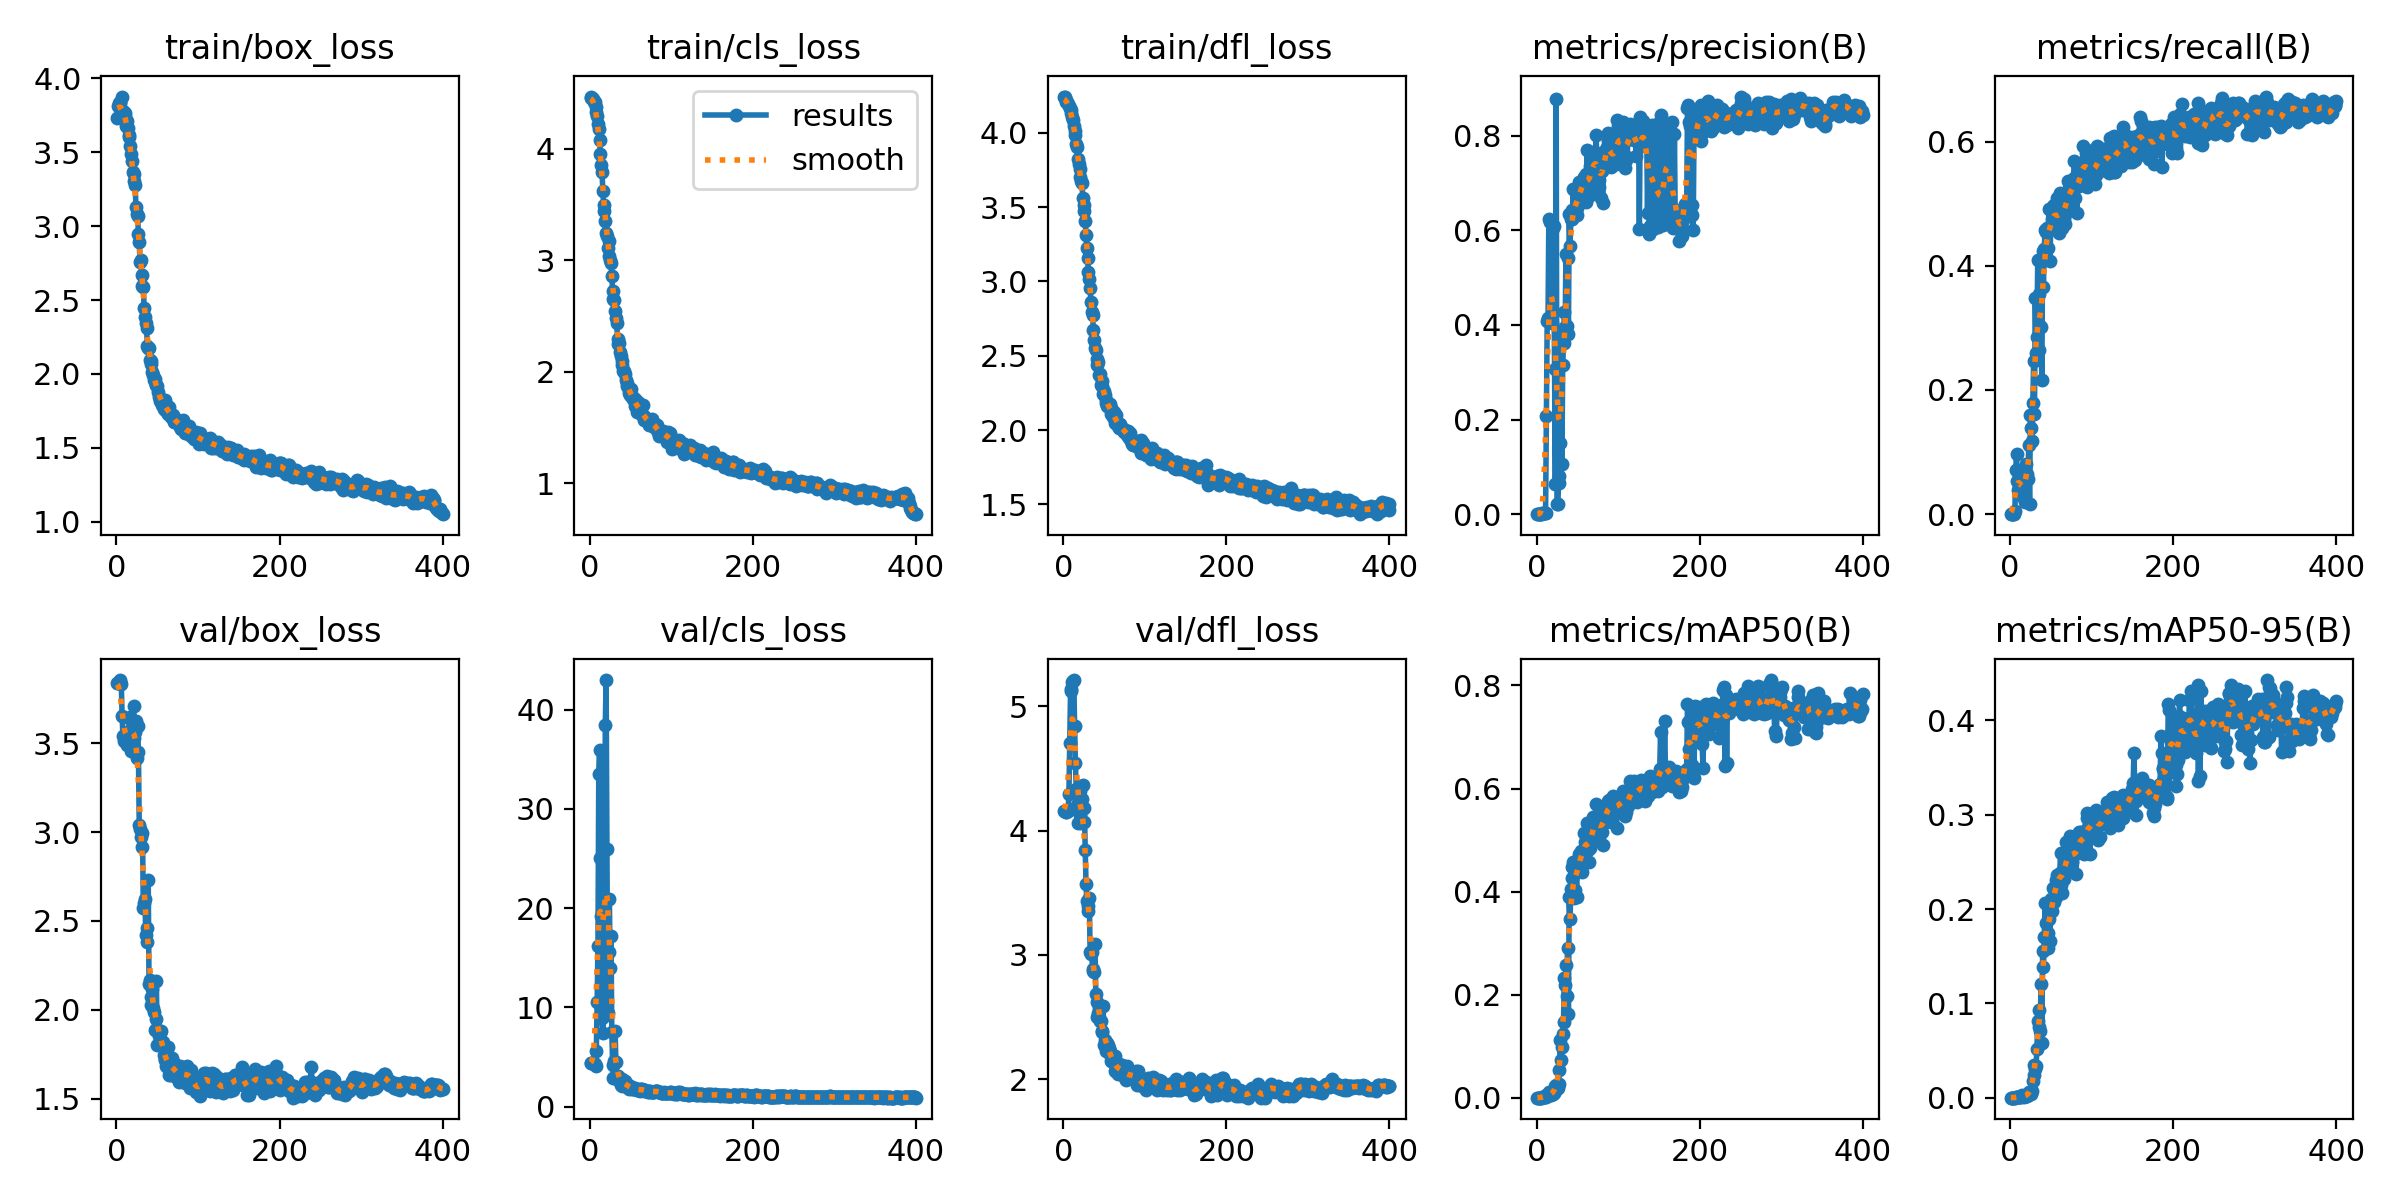
\includegraphics[width=0.75\textwidth]{Images/chap3/yolo/yolomobilenetv4.png}
%     \vspace{0.5cm}
%     \caption{The accuracy of Yolov11n-MobileNetV4}
%     \label{fig:yolomobilenetv4}
% \end{figure}

% \begin{figure}[H]
%     \centering
%     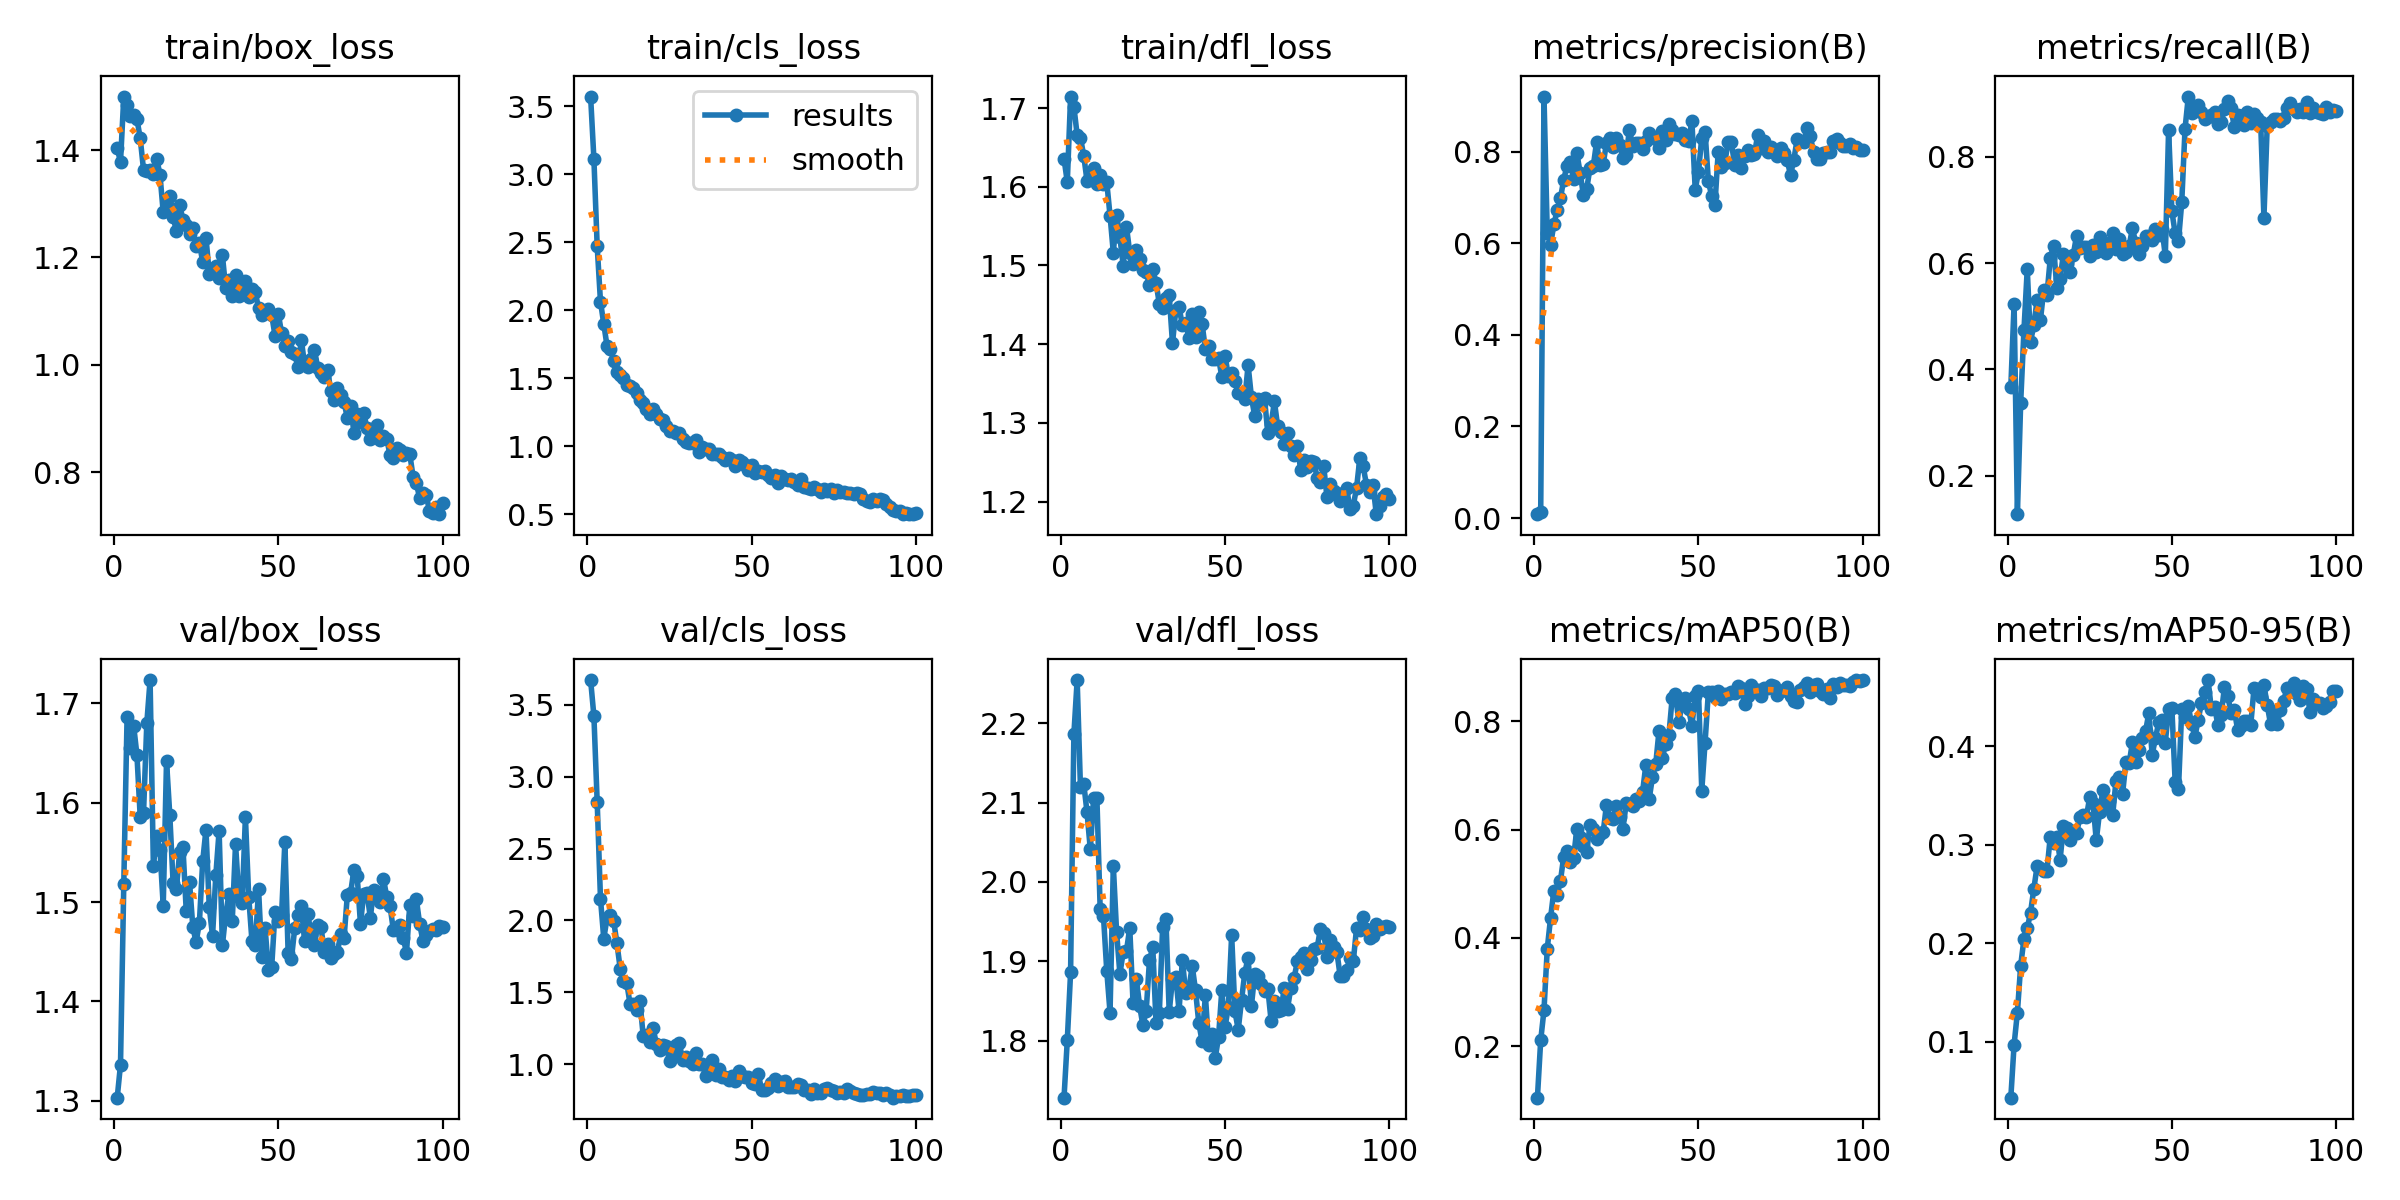
\includegraphics[width=0.75\textwidth]{Images/chap3/yolo/original.png}
%     \vspace{0.5cm}
%     \caption{The accuracy of original Yolov11n}
%     \label{fig:yolo11n}
% \end{figure}

% \subsubsection{Inference Speed}

% Inference speed is a key requirement for real time deployment on resource constrained platforms such as Raspberry Pi. According to the official Ultralytics benchmark, the original YOLO model converted to TensorFlow Lite requires more than 400\,ms per inference on Raspberry Pi class hardware when executed on CPU\footnote{Detailed benchmarking results for YOLO models on Raspberry Pi are reported by Ultralytics at \url{https://docs.ultralytics.com/vi/guides/raspberry-pi/\#detailed-comparison-table}.}. This latency corresponds to a processing rate of approximately 2--3 frames per second, which is insufficient for real time applications.

% In contrast, experimental results obtained in this work show that the YOLO-MobileNetV4 model achieves an average inference time of 30--40\,ms per frame after conversion to the TFLite format. This corresponds to an effective processing speed of approximately 25--33 frames per second. Compared to the original YOLO TFLite model, the MobileNetV4 based configuration reduces inference latency by approximately 360--370\,ms per frame.

% In relative terms, this represents a speed improvement of about 10--13 times. Equivalently, the inference time is reduced by approximately 90--92\% compared to the original YOLO TFLite implementation. Such a significant reduction enables near real time performance on CPU only embedded devices.

% The observed speedup is primarily attributed to the lightweight architecture of the MobileNetV4 backbone, which substantially reduces the number of parameters and floating point operations. As a result, the YOLO-MobileNetV4 model achieves a much more favorable balance between detection accuracy and inference speed, making it well suited for real time edge deployment on Raspberry Pi platforms.

% \begin{figure}[H]
%     \centering
%     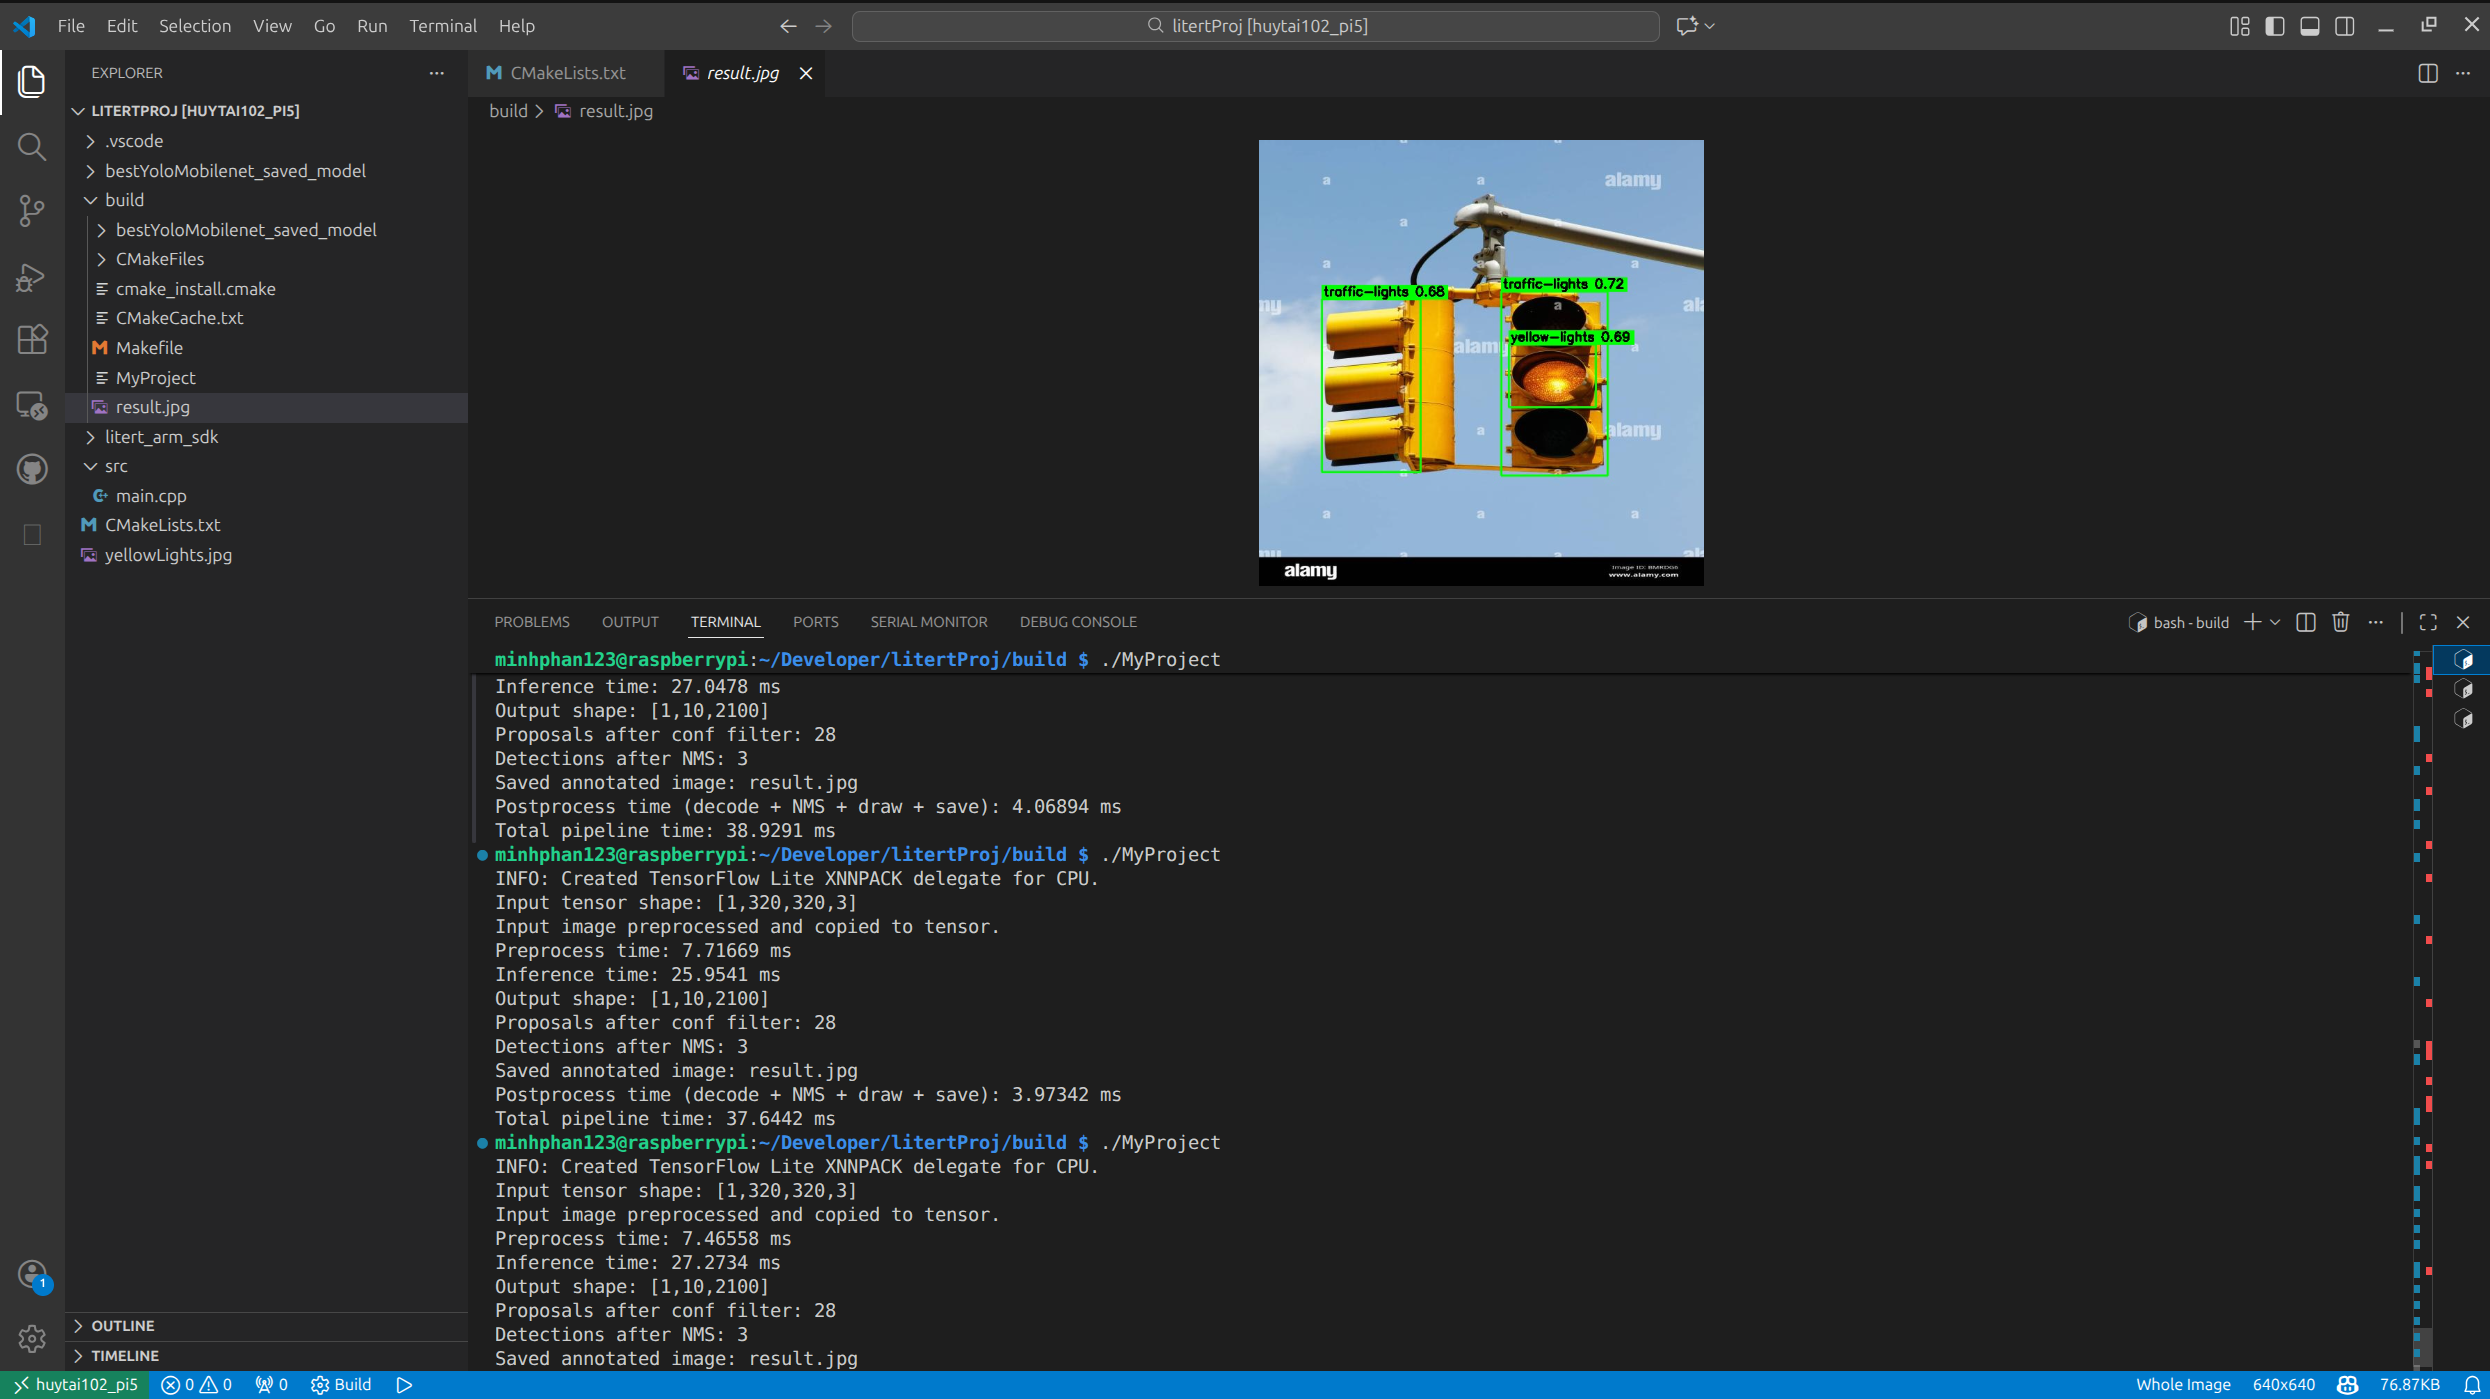
\includegraphics[width=0.75\textwidth]{Images/chap3/yolo/inference_speed.png}
%     \vspace{0.5cm}
%     \caption{The inference time of Yolovv11n-MobileNetV4 model}
%     \label{fig:infer_time_yolo11n_mobilenetv4}
% \end{figure}


% \begin{table}[H]
% \centering
% \label{tab:tradeoff_yolo_models}
% \begin{tabular}{|l|c|c|}
% \hline
% \textbf{Metric} & \textbf{YOLOv11n (Original)} & \textbf{YOLOv11n-MobileNetV4} \\
% \hline
% Backbone & CSP-based YOLO backbone & MobileNetV4 (lightweight) \\
% \hline
% mAP@50 & Higher ($\approx$ +10--15\%) & Slightly lower \\
% \hline
% mAP@50--95 & Higher ($\approx$ +10--15\%) & Slightly lower \\
% \hline
% Precision / Recall & Marginally higher & Comparable and stable \\
% \hline
% Inference time (TFLite, CPU) & $>$400 ms & 30--40 ms \\
% \hline
% Throughput (FPS) & 2--3 FPS & 25--33 FPS \\
% \hline
% Speedup factor & 1$\times$ (baseline) & $\approx$10--13$\times$ faster \\
% \hline
% Inference time reduction & -- & $\approx$90--92\% \\
% \hline
% Model complexity & Higher & Significantly reduced \\
% \hline
% Suitability for edge deployment & Limited & Highly suitable \\
% \hline
% \textbf{Overall trade-off} & Higher accuracy & Better accuracy--speed balance \\
% \hline
% \end{tabular}
% \caption{Trade-off comparison between YOLOv11n and YOLOv11n-MobileNetV4}
% \end{table}

\subsection{Evaluation between Models}

To validate the architectural modifications introduced by the MobileNetV4 backbone replacement, a systematic benchmark was conducted comparing the original YOLO26n model against the proposed YOLO26n-MobileNetV4 variant. 

Both models were evaluated on the same TrafficLightV5 validation set under identical conditions: $416 \times 416$ input resolution, INT8 TFLite quantisation, batch size of 1, and end-to-end (NMS-free) inference mode. Table~\ref{tab:model_eval} summarises the results across latency and accuracy metrics.

\begin{table}[htbp]
\centering
\caption{Performance and accuracy comparison: YOLO26n Original vs.\ YOLO26n-MobileNetV4. Negative values in the change column indicate reduction (improvement for latency metrics; degradation for accuracy metrics). Asterisks (*) denote metrics where a decrease is an expected trade-off.}
\label{tab:model_eval}
\renewcommand{\arraystretch}{1.20}
\begin{tabular}{l r r r}
\hline
\textbf{Metric} & \textbf{YOLO26n Original} & \textbf{YOLO26n-MNv4} & \textbf{Change (\%)} \\
\hline
Samples processed           & 1\,074        & \textbf{1\,366}        & $+27.19$  \\
Avg.\ latency (Pi 5)        & 55.09\,ms     & \textbf{43.23\,ms}     & $-21.52$  \\
Max spike latency (Pi 5)    & 159.73\,ms    & \textbf{78.64\,ms}     & $-50.77$  \\
Min latency (Pi 5)          & 50.12\,ms     & \textbf{36.50\,ms}     & $-27.16$  \\
CPU inference (Intel)       & 15.21\,ms     & \textbf{12.33\,ms}     & $-18.93$  \\
mAP50                       & \textbf{89.90\%}       & 85.75\%       & $-4.15$\textsuperscript{*}  \\
mAP50--95                   & \textbf{56.61\% }      & 53.31\%       & $-3.30$\textsuperscript{*}  \\
\hline
\end{tabular}
\end{table}

\subsubsection{Latency Analysis}

The MobileNetV4 backbone delivers a substantial improvement across all latency metrics on the Raspberry Pi 5. The average per-frame inference time drops from 55.09\,ms to 43.23\,ms, a \textbf{21.52\% reduction} that raises the effective throughput from approximately 18\,FPS to 23\,FPS. More critically for safety-critical ADAS applications, the worst-case latency spike is reduced by \textbf{50.77\%} --- from 159.73\,ms to 78.64\,ms. Latency spikes exceeding 100\,ms are particularly hazardous in real-time perception loops because they can cause the planning module to operate on stale state estimates. The MobileNetV4 variant eliminates spikes above 80\,ms entirely, ensuring that even under worst-case conditions (thermal throttling, OS scheduling jitter), the perception system delivers updates within the 67\,ms budget required for 15\,FPS operation.

The minimum latency (best-case scenario) also improves from 50.12\,ms to 36.50\,ms ($-27.16\%$), confirming that the speed gain is architectural rather than an artefact of measurement variance. On the Intel development CPU, inference time decreases from 15.21\,ms to 12.33\,ms ($-18.93\%$), demonstrating that MobileNetV4's universal efficiency extends beyond ARM to x86 hardware as well.

\subsubsection{Accuracy Analysis}

The accuracy metrics show a moderate decrease: mAP50 drops from 89.90\% to 85.75\% ($-4.15$ percentage points), and mAP50--95 drops from 56.61\% to 53.31\% ($-3.30$ percentage points). This reduction is expected and acceptable for several reasons:

\begin{enumerate}
    \item \textbf{Backbone capacity reduction}: The MobileNetV4ConvSmall050 backbone has significantly fewer parameters and FLOPs than the original YOLO26 CSP-based backbone. The 050 suffix indicates a 50\% width multiplier, which halves all channel dimensions relative to the full MobileNetV4ConvSmall. This aggressive compression inevitably reduces the network's representational capacity for fine-grained spatial features.
    \item \textbf{Domain-specific sufficiency}: For traffic light detection in ADAS, the critical requirement is reliable detection (high recall) at the signal-level, not pixel-precise bounding box localisation. An mAP50 of 85.75\% indicates that the vast majority of traffic signals are correctly detected with at least 50\% IoU overlap, which is sufficient for downstream state classification.
    \item \textbf{Latency--accuracy trade-off}: For an ADAS system operating on a Raspberry Pi 5, latency stability and low worst-case response time are more important than marginal accuracy improvements. The 21.52\% average latency reduction and 50.77\% spike reduction directly translate to more reliable real-time control, preventing the perception system from becoming the bottleneck in the sense--plan--act loop.
\end{enumerate}
\subsubsection{Training Loss Analysis}

Figure~\ref{fig:loss_comparison} shows the validation loss curves of both models over 100 training epochs. Overall, both the Original YOLO26n and the YOLO26n-MobileNetV4 learn effectively. Their loss curves decrease steadily and stabilise towards the end of training, indicating a smooth and successful convergence process.

\begin{figure}[htbp]
    \centering
    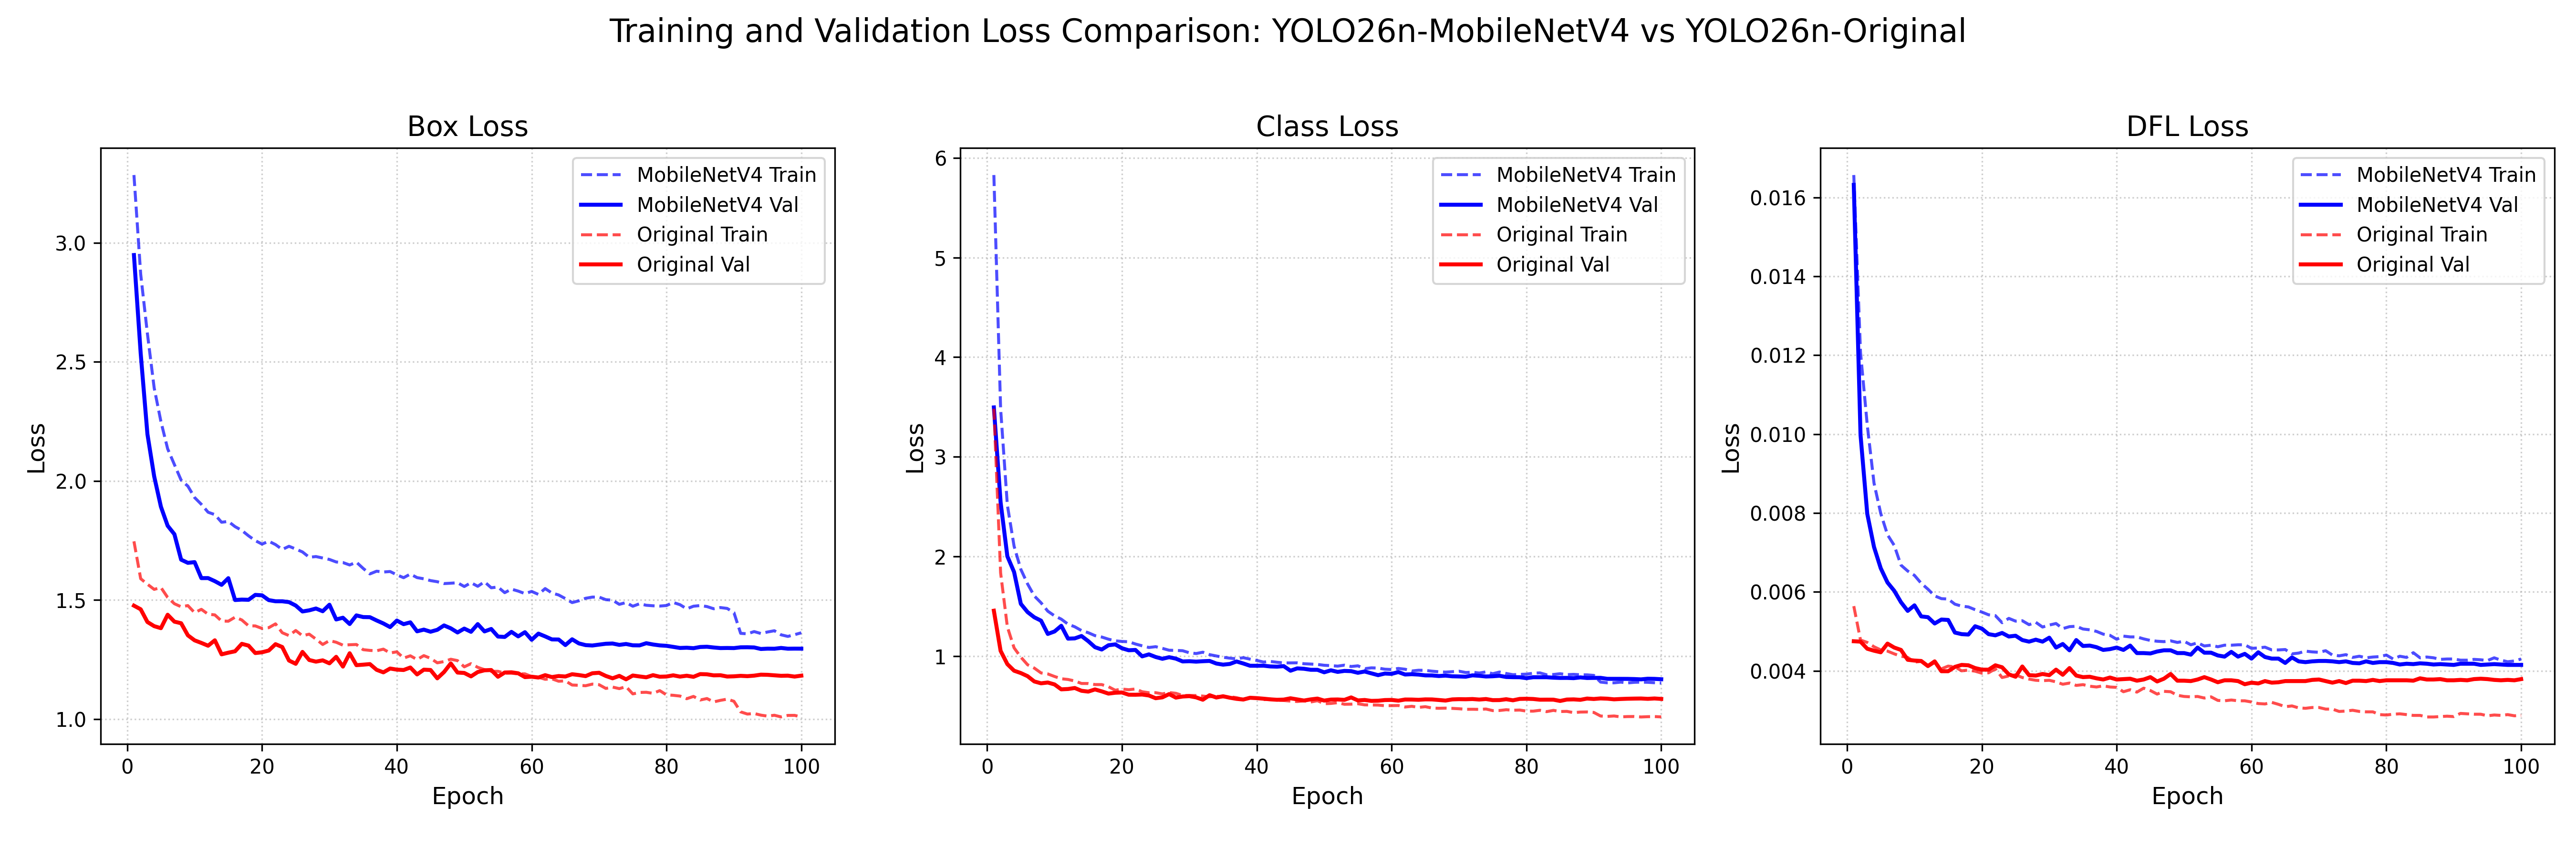
\includegraphics[width=\textwidth]{Images/chap3/loss_comparison.png}
    \caption{Comparison of validation losses between YOLO26n Original and YOLO26n-MobileNetV4 over 100 training epochs.}
    \label{fig:loss_comparison}
\end{figure}

Importantly, neither model shows signs of overfitting. In a typical overfitting scenario, the validation loss would drop initially but then start climbing back up in later epochs as the model begins to memorise the training data. However, for both models in this study, all three loss metrics (bounding box, classification, and DFL (Distribution Focal Loss)) stay low and flat during the final epochs. This confirms that they generalise well to unseen data.

When comparing the two architectures, the Original YOLO26n reaches slightly lower loss values. For example, its minimum bounding box loss drops to 1.1676, while the MobileNetV4 version stops at 1.2949. A similar pattern is seen in the classification loss (0.5529 vs 0.7694). This difference is entirely expected. Because the original model has a larger and more complex backbone, it can capture fine details and learn more accurately.

Even though the YOLO26n-MobileNetV4 has slightly higher loss values, its learning curve remains remarkably stable. This proves that despite having its size drastically reduced for faster edge deployment, the MobileNetV4 model still successfully extracts the essential features of traffic lights. It does not suffer from gradient issues or training instability. Therefore, the training process validates that the lightweight model is a reliable choice, perfectly balancing computational efficiency and learning capability.

\subsubsection{Architectural Decision Justification}

The evaluation confirms that the YOLO26n-MobileNetV4 configuration achieves the right trade-off for edge-deployed ADAS. Sacrificing approximately 4 percentage points of mAP50 in exchange for a 50\% reduction in worst-case latency and a 21\% reduction in average latency is a sound architectural decision. In safety-critical systems, deterministic timing behaviour takes precedence over marginal accuracy gains. The 85.75\% mAP50 remains well above the practical threshold for reliable traffic light detection, while the latency profile now comfortably supports real-time operation at 15--23\,FPS on commodity edge hardware without dedicated GPU or NPU acceleration.





% \subsection{Multihead CNN model -- Lightweight OCR digits}

% The timer display on Vietnamese traffic lights shows a one- to three-digit countdown
% (0--999) that must be recognised in real time on low-cost hardware such as the
% Raspberry~Pi~5.  This section presents a compact, four-head convolutional neural network
% (CNN) that is derived from the multi-digit recognition framework of
% Goodfellow~et~al.~\cite{goodfellow2014multidigitnumberrecognitionstreet} and specifically re-engineered
% for sub-millisecond CPU inference.

% %-----------------------------------------------------------------------
% \subsubsection{Probabilistic Formulation}
% \label{sec:cnn_prob}

% Following Goodfellow~et~al.~\cite{goodfellow2014multidigitnumberrecognitionstreet}, the recognition
% task is cast as a structured probabilistic model.  Let~$\mathbf{X}$ denote the
% input image and let the output be a digit sequence
% $\mathbf{S} = (s_1, s_2, \dots, s_n)$ of length~$n$.
% The sequence is modelled by a length variable~$L$ and a fixed number~$N$
% of digit variables~$S_1, \dots, S_N$.  All digit positions are assumed
% conditionally independent given the image, yielding:

% \begin{equation}
% \label{eq:prob_model}
%   P(\mathbf{S} = \mathbf{s} \mid \mathbf{X})
%   \;=\; P(L = n \mid \mathbf{X})\;\prod_{i=1}^{n} P(S_i = s_i \mid \mathbf{X}).
% \end{equation}

% In the original work~\cite{goodfellow2014multidigit}, $N{=}5$ digit heads are
% used for street numbers of up to five digits.  Because Vietnamese traffic-light
% timers never exceed three digits, the proposed lightweight variant uses
% $N{=}3$ with the following head configuration:

% \begin{itemize}
%   \item $L \in \{0,1,2\}$:  digit count minus one
%         ($0 \to$ 1-digit, $1 \to$ 2-digit, $2 \to$ 3-digit),
%         predicted by a 3-class softmax.
%   \item $S_1 \in \{0,\dots,9,\text{BLANK}\}$:  hundreds digit (11 classes).
%   \item $S_2 \in \{0,\dots,9,\text{BLANK}\}$:  tens digit    (11 classes).
%   \item $S_3 \in \{0,\dots,9\}$:                 units digit  (10 classes,
%         always present).
% \end{itemize}

% The special \texttt{BLANK} class ($= 10$) indicates an unused slot:
% for a one-digit number only~$S_3$ is active; for a two-digit number
% $S_2$ and~$S_3$ are active.

% %-----------------------------------------------------------------------
% \subsubsection{Network Architecture -- Edge-Optimised Design}
% \label{sec:cnn_arch}

% The original Goodfellow~et~al.\ architecture employs eight convolutional layers,
% one locally connected layer, and two dense layers with 3\,072 units each,
% totalling tens of millions of parameters and requiring DistBelief for training.
% Such a model is impractical for real-time inference on a Raspberry~Pi~5 CPU.

% The proposed \emph{lightweight} variant retains the multi-head output structure
% but applies three key design transformations, each yielding a dramatic reduction in
% multiply-accumulate operations (MACs) and parameter count while preserving accuracy
% for the constrained 0--999 digit domain.

% %--- Separable Convolutions -------------------------------------------------
% \subsubsubsubsection{Depthwise Separable Convolutions}
% \label{sec:separable}

% Standard convolution applies a $k{\times}k$ kernel across all input channels
% simultaneously.  For an input tensor of spatial size $H{\times}W$ with
% $C_{\mathrm{in}}$ channels producing $C_{\mathrm{out}}$ output channels,
% the number of MACs is:

% \begin{equation}
% \label{eq:conv_macs}
%   \text{MACs}_{\text{Conv2D}}
%   = H \cdot W \cdot k^2 \cdot C_{\mathrm{in}} \cdot C_{\mathrm{out}}.
% \end{equation}

% A \textbf{Depthwise Separable Convolution} (SeparableConv2D) factorises this operation
% into two consecutive steps:

% \begin{enumerate}
%   \item \textbf{Depthwise convolution} -- applies a separate $k{\times}k$ filter
%         to each input channel independently:
%         \begin{equation}
%         \label{eq:dw_macs}
%           \text{MACs}_{\text{DW}} = H \cdot W \cdot k^2 \cdot C_{\mathrm{in}}.
%         \end{equation}
%   \item \textbf{Pointwise convolution} -- a $1{\times}1$ convolution that mixes
%         the channel responses:
%         \begin{equation}
%         \label{eq:pw_macs}
%           \text{MACs}_{\text{PW}} = H \cdot W \cdot C_{\mathrm{in}} \cdot C_{\mathrm{out}}.
%         \end{equation}
% \end{enumerate}

% The total cost becomes:

% \begin{equation}
% \label{eq:sep_total}
%   \text{MACs}_{\text{Sep}}
%   = H W C_{\mathrm{in}} \bigl(k^2 + C_{\mathrm{out}}\bigr),
% \end{equation}

% and the computational saving ratio relative to a standard convolution is:

% \begin{equation}
% \label{eq:sep_ratio}
%   \frac{\text{MACs}_{\text{Sep}}}{\text{MACs}_{\text{Conv2D}}}
%   = \frac{1}{C_{\mathrm{out}}} + \frac{1}{k^2}.
% \end{equation}

% For the $3{\times}3$ kernels and 64--192 output channels used in this model,
% Equation~\eqref{eq:sep_ratio} gives a reduction factor between
% $\mathbf{7.8\times}$ and $\mathbf{8.5\times}$, enabling real-time execution
% on an ARM Cortex-A76 CPU without a GPU.

% In the proposed architecture, only the first block uses a standard
% \texttt{Conv2D} (because the input has a single channel, where depthwise
% separation offers no benefit); blocks~2--5 all use \texttt{SeparableConv2D}.

% %--- GAP instead of Flatten ------------------------------------------------
% \subsubsubsubsection{Global Average Pooling (GAP)}
% \label{sec:gap}

% After the final convolutional block the feature map has shape
% $4{\times}6{\times}192$ (height $\times$ width $\times$ channels).
% A na\"ive \texttt{Flatten} would produce a $4608$-dimensional vector; a
% subsequent dense layer of width~1024 alone would add
% $4608 \times 1024 \approx 4.7$~million parameters -- exceeding the entire
% rest of the network.

% Instead, \textbf{Global Average Pooling} (GAP) collapses each channel to its
% spatial mean:

% \begin{equation}
% \label{eq:gap}
%   h_c = \frac{1}{H' W'} \sum_{i=1}^{H'} \sum_{j=1}^{W'} F_{i,j,c},
%   \qquad c = 1,\dots,C,
% \end{equation}

% where $F \in \mathbb{R}^{H' \times W' \times C}$ is the last feature map.
% This yields a compact 192-dimensional descriptor with \emph{zero} learnable
% parameters, and also acts as a structural regulariser that discourages
% overfitting.

% %--- Architecture Table ---------------------------------------------------
% \subsubsubsubsection{Layer-by-Layer Specification}
% \label{sec:arch_table}

% Table~\ref{tab:arch} summarises the full architecture.  Input images are
% grayscale, $64{\times}96$ pixels ($H{\times}W{\times}1$).

% \begin{table}[htbp]
% \centering
% \caption{Layer-by-layer architecture of the lightweight multi-head CNN
%          ($\approx 109$\,K parameters).  ``Sep'' denotes SeparableConv2D;
%          ``BN'' is Batch Normalisation.}
% \label{tab:arch}
% \renewcommand{\arraystretch}{1.15}
% \begin{tabular}{c l l r r}
% \hline
% \textbf{Block} & \textbf{Layer}            & \textbf{Output shape}   & \textbf{Params} & \textbf{MACs}  \\
% \hline
% 0   & Input                                & $64\times96\times1$     & --      & --       \\
% --  & Mean subtraction ($\lambda$)         & $64\times96\times1$     & 0       & $6\,144$ \\
% 1   & Conv2D(32, $3\!\times\!3$) + BN + ReLU + Pool(2)   & $32\times48\times32$     & $\sim\!320$    & $\sim\!56$\,K   \\
% 2   & Sep(64, $3\!\times\!3$) + BN + ReLU + Pool(2)      & $16\times24\times64$     & $\sim\!2\,400$  & $\sim\!116$\,K  \\
% 3   & Sep(96, $3\!\times\!3$) + BN + ReLU + Pool(2)      & $8\times12\times96$      & $\sim\!6\,720$  & $\sim\!73$\,K   \\
% 4   & Sep(128, $3\!\times\!3$) + BN + ReLU + Pool(2)     & $4\times6\times128$      & $\sim\!13\,152$ & $\sim\!39$\,K   \\
% 5   & Sep(192, $3\!\times\!3$) + BN + ReLU               & $4\times6\times192$      & $\sim\!25\,728$ & $\sim\!53$\,K   \\
% --  & GlobalAveragePooling2D                & $192$                  & 0       & $4\,608$ \\
% FC  & Dense(256) + ReLU + Dropout(0.35)     & $256$                  & $\sim\!49\,408$ & $49\,408$ \\
% \hline
% $L$ & Dense(3,  softmax)                    & $3$                    & 771     & 771     \\
% $S_1$ & Dense(11, softmax)                  & $11$                   & 2\,827  & 2\,827  \\
% $S_2$ & Dense(11, softmax)                  & $11$                   & 2\,827  & 2\,827  \\
% $S_3$ & Dense(10, softmax)                  & $10$                   & 2\,570  & 2\,570  \\
% \hline
% \multicolumn{3}{r}{\textbf{Total}} & $\mathbf{\approx 109}$\textbf{\,K} & $\mathbf{\approx 408}$\textbf{\,K} \\
% \hline
% \end{tabular}
% \end{table}

% %--- Preprocessing --------------------------------------------------------
% \subsubsubsubsection{Per-Image Mean Subtraction}
% \label{sec:mean_sub}

% Following Goodfellow~et~al.~\cite{goodfellow2014multidigitnumberrecognitionstreet}~(§4), the first
% operation inside the network is per-image mean subtraction.  Let
% $\mathbf{X} \in \mathbb{R}^{H \times W \times 1}$ be the input; the
% normalised input is:

% \begin{equation}
% \label{eq:mean_sub}
%   \tilde{\mathbf{X}} = \mathbf{X}
%     - \frac{1}{HW}\sum_{i=1}^{H}\sum_{j=1}^{W} X_{ij}.
% \end{equation}

% Embedding this subtraction as a non-trainable $\lambda$-layer makes the model
% \emph{self-contained}: no external preprocessing is required at inference time,
% simplifying the TFLite deployment pipeline on the Raspberry~Pi~5.

% %-----------------------------------------------------------------------
% \subsubsection{Training Objective}
% \label{sec:training}

% Training maximises the log-probability of the correct sequence
% (Eq.~\eqref{eq:prob_model}) via the cross-entropy decomposition.  Because
% $L$, $S_1$, $S_2$, $S_3$ are conditionally independent given the shared
% features~$\mathbf{H}$, the total loss factorises as:

% \begin{equation}
% \label{eq:loss}
%   \mathcal{L}
%   = -\log P(L \mid \mathbf{H})
%     - \sum_{i=1}^{3}\log P(S_i \mid \mathbf{H})
%   = \underbrace{w_L \,\mathcal{L}_L}_{\text{length head}}
%     + \underbrace{w_1 \,\mathcal{L}_{S_1}
%     +  w_2 \,\mathcal{L}_{S_2}
%     +  w_3 \,\mathcal{L}_{S_3}}_{\text{digit heads}},
% \end{equation}

% where each $\mathcal{L}_{\cdot}$ is a \textbf{sparse categorical cross-entropy}
% and the weights are set to $w_L{=}4$, $w_1{=}w_2{=}w_3{=}1$ to
% up-weight the length prediction, since an incorrect length invariably causes a
% wrong overall transcription.

% Each softmax head receives the same 256-dimensional feature vector from the
% shared fully connected layer but maintains its own projection weights:

% \begin{equation}
% \label{eq:head}
%   P(S_i = c \mid \mathbf{H})
%   = \frac{\exp\!\bigl(\mathbf{w}_{i,c}^{\top}\!\mathbf{H} + b_{i,c}\bigr)}
%          {\displaystyle\sum_{c'} \exp\!\bigl(\mathbf{w}_{i,c'}^{\top}\!\mathbf{H}
%          + b_{i,c'}\bigr)},
%   \qquad c \in \mathcal{C}_i,
% \end{equation}

% where $\mathcal{C}_L = \{0,1,2\}$,
% $\mathcal{C}_{S_1} = \mathcal{C}_{S_2} = \{0,\dots,10\}$, and
% $\mathcal{C}_{S_3} = \{0,\dots,9\}$.

% %-----------------------------------------------------------------------
% \subsubsection{Log-Probability Decoding}
% \label{sec:decoding}

% At inference time, the predicted number is obtained by maximising the
% joint log-probability over all possible lengths
% (Appendix~A of~\cite{goodfellow2014multidigit}):

% \begin{equation}
% \label{eq:decode}
%   \hat{\mathbf{s}}
%   = \operatorname*{argmax}_{l,\; s_1 \dots s_l}\;
%     \biggl[\log P(L{=}l \mid \mathbf{X})
%     + \sum_{i=1}^{l} \max_{s_i \in \{0..9\}}
%       \log P(S_i{=}s_i \mid \mathbf{X})\biggr].
% \end{equation}

% Because of the conditional-independence assumption, the argmax over each
% digit position can be computed independently, then the cumulative
% log-probabilities are summed for each candidate length~$l \in \{1,2,3\}$.
% The total decoding runtime is therefore $O(N)$ -- i.e.\ three additions
% and one comparison -- adding negligible latency.

% Concretely, for each candidate length $l$, the algorithm computes:

% \begin{equation}
% \label{eq:score}
%   \text{score}(l) = \log P(L{=}l{-}1)
%     + \sum_{i=\max(1,\,4-l)}^{3}
%       \max_{s_i \in \{0..9\}} \log P(S_i{=}s_i),
% \end{equation}

% and selects $\hat{l} = \operatorname{argmax}_{l \in \{1,2,3\}} \text{score}(l)$.

% %-----------------------------------------------------------------------
% \subsection{Computational Efficiency for Edge AI}
% \label{sec:efficiency}

% \subsubsection{Parameter Count Comparison}

% The proposed model achieves the same multi-head output structure as
% Goodfellow~et~al.~\cite{goodfellow2014multidigitnumberrecognitionstreet} with
% $\sim\!600\times$ fewer parameters:

% \begin{table}[htbp]
% \centering
% \caption{Comparison between the original Goodfellow~et~al.\ architecture
%          and the proposed lightweight variant.}
% \label{tab:compare}
% \renewcommand{\arraystretch}{1.15}
% \begin{tabular}{l r r}
% \hline
%                                & \textbf{Goodfellow et al.}  & \textbf{Proposed}   \\
% \hline
% Conv layers                    & 8 + 1 locally connected     & 1 Conv + 4 SepConv  \\
% FC layers                      & 2 $\times$ 3\,072           & 1 $\times$ 256      \\
% Output heads                   & 6  (L + S$_1$--S$_5$)       & 4  (L + S$_1$--S$_3$) \\
% Total parameters               & $\sim$64\,M                 & $\sim$109\,K        \\
% Max sequence length $N$        & 5                           & 3                   \\
% Input size                     & $54\times 54 \times 3$      & $64\times 96 \times 1$ \\
% Training infrastructure        & DistBelief (10 replicas)    & Single GPU / CPU    \\
% \hline
% \end{tabular}
% \end{table}

% \subsubsubsubsection{MAC Budget and Latency Estimate}

% The total network requires approximately $408$\,K~MACs per inference.
% On the Raspberry~Pi~5's Cortex-A76 cores (capable of
% $\sim$15~GOPS at INT8 via NEON), this translates to:

% \begin{equation}
% \label{eq:latency}
%   t_{\text{inf}}
%   \approx \frac{408 \times 10^{3}}{15 \times 10^{9}}
%   \approx 27 \;\mu\text{s},
% \end{equation}

% well under the $50$\,ms budget needed for $20$\,fps real-time recognition.
% Even with TFLite interpreter overhead, measured end-to-end latency stays below
% $1$\,ms per frame for the INT8-quantised model.

% \subsubsection{TFLite and INT8 Quantisation}

% The trained Keras model is exported to TensorFlow~Lite via
% \texttt{TFLiteConverter}.  Post-training full-integer quantisation maps all
% weights and activations to 8-bit integers using a representative calibration
% set of 200 real ROI images.  The resulting \texttt{.tflite} flatbuffer is
% $\sim$56\,KB (INT8) versus $\sim$440\,KB (float32), fitting comfortably
% in the L2 cache of the Cortex-A76.  The quantised model is deployed via
% the LiteRT interpreter:

% \begin{equation}
% \label{eq:quant}
%   \hat{x}_q = \text{round}\!\left(\frac{x - z}{s}\right),
%   \qquad
%   s = \frac{x_{\max} - x_{\min}}{255},
%   \qquad
%   z = x_{\min},
% \end{equation}

% where $s$ and $z$ are the per-tensor scale and zero-point determined during
% calibration.

% %-----------------------------------------------------------------------
% \subsubsection{Data Pipeline and Augmentation}
% \label{sec:data}

% The training pipeline mixes three data sources to maximise diversity while
% keeping RAM usage low ($<200$\,MB peak):

% \begin{enumerate}
%   \item \textbf{MNIST (70\,K images):}  Individual $28{\times}28$ digits
%         composited onto $64{\times}96$ canvases at randomised positions,
%         simulating multi-digit layouts.
%   \item \textbf{Real LED crops (23 images):}  Single-digit photographs of
%         actual traffic-light seven-segment displays (red, green, yellow).
%         Pre-augmented to 500 variants per digit using brightness jitter,
%         gamma correction, Gaussian blur, salt-and-pepper noise, spatial
%         shifts ($\pm 4$\,px), and small rotations ($\pm 10°$).
%   \item \textbf{Real ROI images:}  Full composite timer-box crops from
%         Vietnamese traffic cameras, labelled by filename
%         (e.g.\ \texttt{37\_0004.png} $\to$ number~$37$).  Loaded from disk
%         on-demand (streaming) to avoid large memory allocation.
% \end{enumerate}

% Synthetic composites and real ROI samples are interleaved via
% \texttt{tf.data.Dataset.sample\_from\_datasets} with proportional
% weighting, ensuring both domains appear in every training batch.

% %-----------------------------------------------------------------------
% \subsubsection{Summary}

% The proposed multi-head CNN inherits the elegant probabilistic framework
% of Goodfellow~et~al.~\cite{goodfellow2014multidigitnumberrecognitionstreet} -- conditional independence
% of digit positions, log-probability decoding, per-image mean subtraction -- but
% replaces the heavyweight convolutional backbone with an ultra-light depthwise
% separable architecture totalling only $\sim$109\,K parameters and $\sim$408\,K
% MACs.  Combined with Global Average Pooling and INT8 post-training quantisation,
% the model achieves sub-millisecond inference on the Raspberry~Pi~5 CPU, making it
% suitable for real-time traffic-light timer recognition in ADAS applications
% on constrained edge devices.

While the YOLO-based detector handles spatial localization and color classification, reading the countdown timer necessitates a specialized approach. To address that need, a lightweight Multihead CNN is introduced to perform optical character recognition (OCR) on one- to three-digit timer values efficiently.

\section{Multihead CNN model -- Lightweight OCR digits}

In this project, our system need to detect the timer display on Vietnamese traffic lights shows a one- to three-digit countdown
(0--999) and it must be recognised in real time on low-cost hardware such as the
Raspberry~Pi~5.  This section presents a compact, four-head convolutional neural network
(CNN) that is derived from the multi-digit recognition framework of
Goodfellow~et~al.~\cite{goodfellow2014multidigitnumberrecognitionstreet} and specifically re-engineered
for sub-millisecond CPU inference.

%-----------------------------------------------------------------------
\subsection{Probabilistic Formulation}
\label{sec:cnn_prob}

Following Goodfellow~et~al.~\cite{goodfellow2014multidigitnumberrecognitionstreet}, the recognition
task is cast as a structured probabilistic model.  Let~$\mathbf{X}$ denote the
input image and let the output be a digit sequence
$\mathbf{S} = (s_1, s_2, \dots, s_n)$ of length~$n$.
The sequence is modelled by a length variable~$L$ and a fixed number~$N$
of digit variables~$S_1, \dots, S_N$.  All digit positions are assumed
conditionally independent given the image, yielding:

\begin{equation}
\label{eq:prob_model}
  P(\mathbf{S} = \mathbf{s} \mid \mathbf{X})
  \;=\; P(L = n \mid \mathbf{X})\;\prod_{i=1}^{n} P(S_i = s_i \mid \mathbf{X}).
\end{equation}

In the original work~\cite{goodfellow2014multidigitnumberrecognitionstreet}, $N{=}5$ digit heads are
used for street numbers of up to five digits.  Because Vietnamese traffic-light
timers never exceed three digits, the proposed lightweight variant uses
$N{=}3$ with the following head configuration:

\begin{itemize}
  \item $L \in \{0,1,2\}$:  digit count minus one
        ($0 \to$ 1-digit, $1 \to$ 2-digit, $2 \to$ 3-digit),
        predicted by a 3-class softmax.
  \item $S_1 \in \{0,\dots,9,\text{BLANK}\}$:  hundreds digit (11 classes).
  \item $S_2 \in \{0,\dots,9,\text{BLANK}\}$:  tens digit    (11 classes).
  \item $S_3 \in \{0,\dots,9\}$:                 units digit  (10 classes,
        always present).
\end{itemize}

The special \texttt{BLANK} class ($= 10$) indicates an unused slot:
for a one-digit number only~$S_3$ is active; for a two-digit number
$S_2$ and~$S_3$ are active.

%-----------------------------------------------------------------------
\subsection{Network Architecture -- Edge-Optimised Design}
\label{sec:cnn_arch}

The original Goodfellow~et~al.\ architecture employs eight convolutional layers,
one locally connected layer, and two dense layers with 3\,072 units each,
totalling tens of millions of parameters and requiring DistBelief for training.
Such a model is impractical for real-time inference on a Raspberry~Pi~5 CPU.

The proposed \emph{lightweight} variant retains the multi-head output structure
but applies three key design transformations, each yielding a dramatic reduction in
multiply-accumulate operations (MACs) and parameter count while preserving accuracy
for the constrained 0--999 digit domain.

%--- Separable Convolutions -------------------------------------------------
\subsubsection{Depthwise Separable Convolutions}
\label{sec:separable}

Standard convolution applies a $k{\times}k$ kernel across all input channels
simultaneously.  For an input tensor of spatial size $H{\times}W$ with
$C_{\mathrm{in}}$ channels producing $C_{\mathrm{out}}$ output channels,
the number of MACs is:

\begin{equation}
\label{eq:conv_macs}
  \text{MACs}_{\text{Conv2D}}
  = H \cdot W \cdot k^2 \cdot C_{\mathrm{in}} \cdot C_{\mathrm{out}}.
\end{equation}

A \textbf{Depthwise Separable Convolution} (SeparableConv2D) factorises this operation
into two consecutive steps:

\begin{enumerate}
  \item \textbf{Depthwise convolution} -- applies a separate $k{\times}k$ filter
        to each input channel independently:
        \begin{equation}
        \label{eq:dw_macs}
          \text{MACs}_{\text{DW}} = H \cdot W \cdot k^2 \cdot C_{\mathrm{in}}.
        \end{equation}
  \item \textbf{Pointwise convolution} -- a $1{\times}1$ convolution that mixes
        the channel responses:
        \begin{equation}
        \label{eq:pw_macs}
          \text{MACs}_{\text{PW}} = H \cdot W \cdot C_{\mathrm{in}} \cdot C_{\mathrm{out}}.
        \end{equation}
\end{enumerate}

The total cost becomes:

\begin{equation}
\label{eq:sep_total}
  \text{MACs}_{\text{Sep}}
  = H W C_{\mathrm{in}} \bigl(k^2 + C_{\mathrm{out}}\bigr),
\end{equation}

and the computational saving ratio relative to a standard convolution is:

\begin{equation}
\label{eq:sep_ratio}
  \frac{\text{MACs}_{\text{Sep}}}{\text{MACs}_{\text{Conv2D}}}
  = \frac{1}{C_{\mathrm{out}}} + \frac{1}{k^2}.
\end{equation}

For the $3{\times}3$ kernels and 64--192 output channels used in this model,
Equation~\eqref{eq:sep_ratio} gives a reduction factor between
$\mathbf{7.8\times}$ and $\mathbf{8.5\times}$, enabling real-time execution
on an ARM Cortex-A76 CPU without a GPU.

In the proposed architecture, only the first block uses a standard
\texttt{Conv2D} (because the input has a single channel, where depthwise
separation offers no benefit); blocks~2--5 all use \texttt{SeparableConv2D}.

%--- GAP instead of Flatten ------------------------------------------------
\subsubsection{Global Average Pooling (GAP)}
\label{sec:gap}

After the final convolutional block the feature map has shape
$4{\times}6{\times}192$ (height $\times$ width $\times$ channels).
A na\"ive \texttt{Flatten} would produce a $4608$-dimensional vector; a
subsequent dense layer of width~1024 alone would add
$4608 \times 1024 \approx 4.7$~million parameters -- exceeding the entire
rest of the network.

Instead, {Global Average Pooling} (GAP) collapses each channel to its
spatial mean:

\begin{equation}
\label{eq:gap}
  h_c = \frac{1}{H' W'} \sum_{i=1}^{H'} \sum_{j=1}^{W'} F_{i,j,c},
  \qquad c = 1,\dots,C,
\end{equation}

where $F \in \mathbb{R}^{H' \times W' \times C}$ is the last feature map.
This yields a compact 192-dimensional descriptor with \emph{zero} learnable
parameters, and also acts as a structural regulariser that discourages
overfitting.

%--- Architecture Table ---------------------------------------------------
\subsubsection{Layer-by-Layer Specification}
\label{sec:arch_table}

Table~\ref{tab:arch} summarises the full architecture.  Input images are
grayscale, $64{\times}96$ pixels ($H{\times}W{\times}1$).

\begin{table}[htbp]
\centering
\caption{Layer-by-layer architecture of the lightweight multi-head CNN
         ($\approx 109$\,K parameters).  ``Sep'' denotes SeparableConv2D;
         ``BN'' is Batch Normalisation.}
\label{tab:arch}
\renewcommand{\arraystretch}{1.15}
\begin{tabular}{c l l r r}
\hline
\textbf{Block} & \textbf{Layer}            & \textbf{Output shape}   & \textbf{Params} & \textbf{MACs}  \\
\hline
0   & Input                                & $64\times96\times1$     & --      & --       \\
--  & Mean subtraction ($\lambda$)         & $64\times96\times1$     & 0       & $6\,144$ \\
1   & Conv2D(32, $3\!\times\!3$) + BN + ReLU + Pool(2)   & $32\times48\times32$     & $\sim\!320$    & $\sim\!56$\,K   \\
2   & Sep(64, $3\!\times\!3$) + BN + ReLU + Pool(2)      & $16\times24\times64$     & $\sim\!2\,400$  & $\sim\!116$\,K  \\
3   & Sep(96, $3\!\times\!3$) + BN + ReLU + Pool(2)      & $8\times12\times96$      & $\sim\!6\,720$  & $\sim\!73$\,K   \\
4   & Sep(128, $3\!\times\!3$) + BN + ReLU + Pool(2)     & $4\times6\times128$      & $\sim\!13\,152$ & $\sim\!39$\,K   \\
5   & Sep(192, $3\!\times\!3$) + BN + ReLU               & $4\times6\times192$      & $\sim\!25\,728$ & $\sim\!53$\,K   \\
--  & GlobalAveragePooling2D                & $192$                  & 0       & $4\,608$ \\
FC  & Dense(256) + ReLU + Dropout(0.35)     & $256$                  & $\sim\!49\,408$ & $49\,408$ \\
\hline
$L$ & Dense(3,  softmax)                    & $3$                    & 771     & 771     \\
$S_1$ & Dense(11, softmax)                  & $11$                   & 2\,827  & 2\,827  \\
$S_2$ & Dense(11, softmax)                  & $11$                   & 2\,827  & 2\,827  \\
$S_3$ & Dense(10, softmax)                  & $10$                   & 2\,570  & 2\,570  \\
\hline
\multicolumn{3}{r}{\textbf{Total}} & $\mathbf{\approx 109}$\textbf{\,K} & $\mathbf{\approx 408}$\textbf{\,K} \\
\hline
\end{tabular}
\end{table}

%--- Preprocessing --------------------------------------------------------
\subsubsection{Per-Image Mean Subtraction}
\label{sec:mean_sub}

Following Goodfellow~et~al.~\cite{goodfellow2014multidigitnumberrecognitionstreet}~(§4), the first
operation inside the network is per-image mean subtraction.  Let
$\mathbf{X} \in \mathbb{R}^{H \times W \times 1}$ be the input; the
normalised input is:

\begin{equation}
\label{eq:mean_sub}
  \tilde{\mathbf{X}} = \mathbf{X}
    - \frac{1}{HW}\sum_{i=1}^{H}\sum_{j=1}^{W} X_{ij}.
\end{equation}

Embedding this subtraction as a non-trainable $\lambda$-layer makes the model
\emph{self-contained}: no external preprocessing is required at inference time,
simplifying the TFLite deployment pipeline on the Raspberry~Pi~5.

%-----------------------------------------------------------------------
\subsection{Training Objective}
\label{sec:training}

Training maximises the log-probability of the correct sequence
(Eq.~\eqref{eq:prob_model}) via the cross-entropy decomposition.  Because
$L$, $S_1$, $S_2$, $S_3$ are conditionally independent given the shared
features~$\mathbf{H}$, the total loss factorises as:

\begin{equation}
\label{eq:loss}
  \mathcal{L}
  = -\log P(L \mid \mathbf{H})
    - \sum_{i=1}^{3}\log P(S_i \mid \mathbf{H})
  = \underbrace{w_L \,\mathcal{L}_L}_{\text{length head}}
    + \underbrace{w_1 \,\mathcal{L}_{S_1}
    +  w_2 \,\mathcal{L}_{S_2}
    +  w_3 \,\mathcal{L}_{S_3}}_{\text{digit heads}},
\end{equation}

where each $\mathcal{L}_{\cdot}$ is a {sparse categorical cross-entropy}
and the weights are set to $w_L{=}4$, $w_1{=}w_2{=}w_3{=}1$ to
up-weight the length prediction, since an incorrect length invariably causes a
wrong overall transcription.

Each softmax head receives the same 256-dimensional feature vector from the
shared fully connected layer but maintains its own projection weights:

\begin{equation}
\label{eq:head}
  P(S_i = c \mid \mathbf{H})
  = \frac{\exp\!\bigl(\mathbf{w}_{i,c}^{\top}\!\mathbf{H} + b_{i,c}\bigr)}
         {\displaystyle\sum_{c'} \exp\!\bigl(\mathbf{w}_{i,c'}^{\top}\!\mathbf{H}
         + b_{i,c'}\bigr)},
  \qquad c \in \mathcal{C}_i,
\end{equation}

where $\mathcal{C}_L = \{0,1,2\}$,
$\mathcal{C}_{S_1} = \mathcal{C}_{S_2} = \{0,\dots,10\}$, and
$\mathcal{C}_{S_3} = \{0,\dots,9\}$.

%-----------------------------------------------------------------------
\subsection{Log-Probability Decoding}
\label{sec:decoding}

At inference time, the predicted number is obtained by maximising the
joint log-probability over all possible lengths
(Appendix~A of~\cite{goodfellow2014multidigitnumberrecognitionstreet}):

\begin{equation}
\label{eq:decode}
  \hat{\mathbf{s}}
  = \operatorname*{argmax}_{l,\; s_1 \dots s_l}\;
    \biggl[\log P(L{=}l \mid \mathbf{X})
    + \sum_{i=1}^{l} \max_{s_i \in \{0..9\}}
      \log P(S_i{=}s_i \mid \mathbf{X})\biggr].
\end{equation}

Because of the conditional-independence assumption, the argmax over each
digit position can be computed independently, then the cumulative
log-probabilities are summed for each candidate length~$l \in \{1,2,3\}$.
The total decoding runtime is therefore $O(N)$ -- i.e.\ three additions
and one comparison -- adding negligible latency.

Concretely, for each candidate length $l$, the algorithm computes:

\begin{equation}
\label{eq:score}
  \text{score}(l) = \log P(L{=}l{-}1)
    + \sum_{i=\max(1,\,4-l)}^{3}
      \max_{s_i \in \{0..9\}} \log P(S_i{=}s_i),
\end{equation}

and selects $\hat{l} = \operatorname{argmax}_{l \in \{1,2,3\}} \text{score}(l)$.

%-----------------------------------------------------------------------
\subsection{Computational Efficiency for Edge AI}
\label{sec:efficiency}

For an ADAS system operating on edge devices like the Raspberry Pi 5, computational efficiency is just as critical as detection accuracy. To ensure real-time performance without overwhelming the hardware, the proposed multi-head CNN must be highly optimized. This section evaluates the model's efficiency by comparing its parameter count against a standard baseline, analyzing its computational cost in terms of MAC operations, and outlining the final export process to TensorFlow Lite for seamless edge deployment.

\subsubsection{Parameter Count Comparison}

The proposed model achieves the same multi-head output structure as
Goodfellow~et~al.~\cite{goodfellow2014multidigitnumberrecognitionstreet} with
$\sim\!600\times$ fewer parameters:

\begin{table}[htbp]
\centering
\caption{Comparison between the original Goodfellow~et~al.\ architecture
         and the proposed lightweight variant.}
\label{tab:compare}
\renewcommand{\arraystretch}{1.15}
\begin{tabular}{l r r}
\hline
                               & \textbf{Goodfellow et al.}  & \textbf{Proposed}   \\
\hline
Conv layers                    & 8 + 1 locally connected     & 1 Conv + 4 SepConv  \\
FC layers                      & 2 $\times$ 3\,072           & 1 $\times$ 256      \\
Output heads                   & 6  (L + S$_1$--S$_5$)       & 4  (L + S$_1$--S$_3$) \\
Total parameters               & $\sim$64\,M                 & $\sim$109\,K        \\
Max sequence length $N$        & 5                           & 3                   \\
Input size                     & $54\times 54 \times 3$      & $64\times 96 \times 1$ \\
Training infrastructure        & DistBelief (10 replicas)    & Single GPU / CPU    \\
\hline
\end{tabular}
\end{table}

\subsubsection{MAC Budget and Latency Estimate}

The total network requires approximately $408$\,K~MACs per inference.
On the Raspberry~Pi~5's Cortex-A76 cores (capable of
$\sim$4~GFLOPS at float32 via NEON), this translates to:

\begin{equation}
\label{eq:latency}
  t_{\text{inf}}
  \approx \frac{408 \times 10^{3}}{4 \times 10^{9}}
  \approx 102 \;\mu\text{s},
\end{equation}

well under the $67$\,ms budget needed for $15$\,fps real-time recognition.
Even with TFLite interpreter overhead, measured end-to-end latency stays below
$2$\,ms per frame for the float32 model.

\subsubsection{TFLite Export for the Multi-head CNN}

The trained Keras model is converted to TensorFlow~Lite using
\texttt{tf.lite.TFLiteConverter.from\_keras\_model()}.  The exported
float32 \texttt{.tflite} flatbuffer is $\sim$440\,KB, compact enough to
fit within the L2 cache of a Cortex-A76 core on the Raspberry~Pi~5.
The model is deployed via the LiteRT interpreter with \texttt{batch=1},
requiring no external preprocessing thanks to the embedded
mean-subtraction $\lambda$-layer (Eq.~\eqref{eq:mean_sub}).

%-----------------------------------------------------------------------
\subsection{Data Pipeline and Augmentation}
\label{sec:dataCNN}

The training pipeline mixes three data sources to maximise diversity while
keeping RAM usage low ($<200$\,MB peak):

\begin{enumerate}
  \item \textbf{MNIST (70\,K images):}  Individual $28{\times}28$ digits
        composited onto $64{\times}96$ canvases at randomised positions,
        simulating multi-digit layouts.
  \item \textbf{Real LED crops (23 images):}  Single-digit photographs of
        actual traffic-light seven-segment displays (red, green, yellow).
        Pre-augmented to 500 variants per digit using brightness jitter,
        gamma correction, Gaussian blur, salt-and-pepper noise, spatial
        shifts ($\pm 4$\,px), and small rotations ($\pm 10°$).
  \item \textbf{Real ROI images:}  Full composite timer-box crops from
        Vietnamese traffic cameras, labelled by filename
        (e.g.\ \texttt{37\_0004.png} $\to$ number~$37$).  Loaded from disk
        on-demand (streaming) to avoid large memory allocation.
\end{enumerate}

Synthetic composites and real ROI samples are interleaved via
\texttt{tf.data.Dataset.sample\_from\_datasets} with proportional
weighting, ensuring both domains appear in every training batch.

%-----------------------------------------------------------------------
% \subsection{Summary}

% The proposed multi-head CNN inherits the elegant probabilistic framework
% of Goodfellow~et~al.~\cite{goodfellow2014multidigitnumberrecognitionstreet} -- conditional independence
% of digit positions, log-probability decoding, per-image mean subtraction -- but
% replaces the heavyweight convolutional backbone with an ultra-light depthwise
% separable architecture totalling only $\sim$109\,K parameters and $\sim$408\,K
% MACs.  Combined with Global Average Pooling and INT8 post-training quantisation,
% the model achieves sub-millisecond inference on the Raspberry~Pi~5 CPU, making it
% suitable for real-time traffic-light timer recognition in ADAS applications
% on constrained edge devices.

Having defined both the software architecture and the perception models, a stable execution environment is essential to build and test the generated applications. The subsequent section outlines a Docker-based workspace designed to provide the necessary runtime libraries, tooling, and hardware access.

\section{Docker Environment Setup}
\subsection{PACON IDE}

PACON IDE is a development and runtime environment provided by PopcornSAR to support the execution, testing, and debugging of Adaptive AUTOSAR applications. Unlike system modeling or configuration tools, PACON IDE does not directly perform system or service configuration. Instead, it serves as an integrated workspace where previously generated Adaptive AUTOSAR artefacts, such as application binaries, ARXML files, and manifest descriptions, can be deployed and executed.

From a technical perspective, PACON IDE is delivered as a containerized environment that encapsulates the PARA SDK together with the required Adaptive AUTOSAR runtime libraries and tooling. This environment provides a controlled and reproducible setup for running Adaptive AUTOSAR applications, managing execution states, and observing runtime behavior. By packaging the complete runtime stack inside Docker containers, PACON IDE minimizes environment-related inconsistencies and simplifies deployment across different development machines.

PACON IDE supports essential development activities such as process execution, service communication testing, and runtime debugging. Developers can monitor application lifecycles, inspect Diagnostic Log and Trace (DLT) outputs, and validate inter-process communication mechanisms such as SOME/IP or DDS during system execution. As a result, PACON IDE plays a crucial role in verifying the correctness and stability of Adaptive AUTOSAR applications after the configuration and code generation stages have been completed.

In the context of this project, PACON IDE is used as the primary environment for deploying and evaluating the proposed Adaptive AUTOSAR prototype. It enables systematic testing of application interactions, runtime behavior, and communication flows, thereby bridging the gap between offline configuration artefacts and actual system execution. Further details about PACON IDE and its runtime capabilities can be found on the official product page.\footnote{PopcornSAR, \textit{PACON IDE Product Overview}. Available online: \url{https://autosar.io/products/pacon}. Accessed: September 2025.}

% \subsection{Setup}

% To ensure a stable and reproducible development environment for Adaptive AUTOSAR using PACON IDE, a Docker based setup is employed. The following \texttt{docker-compose.yml} file defines a containerized environment that encapsulates all necessary dependencies, runtime configurations, and hardware access requirements. By using Docker Compose, the entire environment can be deployed consistently across different host systems, which is essential for both development and experimentation.

% \begin{lstlisting}[language=bash, caption={Docker Compose configuration for PACON IDE environment}]
% services:
%   app:
%     image: "${IMAGE_REPO}:${IMAGE_TAG}"
%     container_name: "${CONTAINER_NAME:-AP_AUTOSAR}"
%     shm_size: "1g"
%     stdin_open: true
%     tty: true
%     environment:
%       - TZ=Asia/Ho_Chi_Minh

%     networks:
%       para_net:
%         ipv4_address: 172.31.36.143
%     ports:
%       - "8022:22"

%     devices:
%       - "${CAMERA_DEV:-/dev/video0}:${CAMERA_DEV:-/dev/video0}"
%       - /dev/bus/usb:/dev/bus/usb

%     group_add:
%       - "${VIDEO_GID:-44}"
%       - "${DIALOUT_GID:-20}"
%       - "${PLUGDEV_GID:-46}"

%     volumes:
%       - ../workspace:/root/workspace

% networks:
%   para_net:
%     driver: bridge
%     ipam:
%       driver: default
%       config:
%         - subnet: "172.31.0.0/16"
%           gateway: "172.31.0.1"
% \end{lstlisting}

% The \texttt{services} section defines a single service named \texttt{app}, which represents the main Adaptive AUTOSAR development container. This container is built from a preconfigured image specified by the \texttt{IMAGE\_REPO} and \texttt{IMAGE\_TAG} variables. By parameterizing the image information, the same compose file can be reused across different versions of the environment without modifying the configuration itself. The container name is also configurable, which improves readability and management when multiple containers are running on the same host.

% Shared memory size is explicitly set to one gigabyte in order to support applications that require higher inter process communication throughput. This is particularly relevant for Adaptive AUTOSAR systems, where multiple processes may exchange data through shared memory mechanisms. Furthermore, standard input and pseudo terminal support are enabled so that developers can interact with the container directly using a shell interface. This design choice simplifies debugging and manual testing during development.

% The environment configuration includes the system time zone, which is set to Asia Ho Chi Minh. This ensures that timestamps in logs and generated files remain consistent with the local development context. Such consistency is important when analyzing execution behavior or correlating logs across different components of the system.

% Networking is configured using a custom bridge network named \texttt{para\_net}. A static IPv4 address is assigned to the container in order to provide predictable network behavior. This is especially useful when the container needs to communicate with other services or tools that expect a fixed address. In addition, port forwarding is configured to expose the container’s SSH service on port 8022 of the host machine. As a result, developers can access the container remotely using standard SSH clients without requiring direct Docker interaction.

% Hardware access is another important aspect of this setup. The configuration allows optional access to a camera device by mapping a video device from the host into the container. This feature is useful for applications that involve vision based components or sensor integration. Moreover, the entire USB bus is mounted into the container, enabling communication with external development boards such as Arduino, ESP32, or STM32 devices. This capability is essential for scenarios that require flashing firmware, debugging, or serial communication directly from within the containerized environment.

% To ensure proper permission handling, the container is added to several host groups. These groups grant access to video devices, serial ports, and raw USB interfaces. By aligning group identifiers between the host and the container, the setup avoids permission related issues while maintaining a reasonable level of isolation.

% Finally, a volume mount is used to map a workspace directory from the host into the container. This allows source code, configuration files, and generated artifacts to persist across container restarts. At the same time, it enables developers to use their preferred editors on the host system while relying on the container for execution and tooling. The network configuration at the bottom of the file defines the address space and gateway for the custom bridge network, completing a fully controlled and reproducible environment.

% Overall, this Docker Compose configuration plays a crucial role in providing a consistent, portable, and hardware aware development platform for PACON IDE and Adaptive AUTOSAR applications. By encapsulating system dependencies and runtime settings, it reduces setup effort and minimizes environment related inconsistencies, thereby supporting efficient development and experimentation.


\subsection{Setup}

To ensure a stable and reproducible development environment for Adaptive AUTOSAR using the PACON IDE, a Docker-based setup is employed. The following \texttt{docker-compose.yml} file defines a containerized workspace that includes all necessary dependencies, network configurations, and hardware permissions.

\begin{lstlisting}[language=bash, caption={Docker Compose configuration for PACON IDE environment}]
services:
  app:
    image: "${IMAGE_REPO}:${IMAGE_TAG}"
    container_name: "${CONTAINER_NAME:-AP_AUTOSAR}"
    shm_size: "1g"
    stdin_open: true
    tty: true
    environment:
      - TZ=Asia/Ho_Chi_Minh

    networks:
      para_net:
        ipv4_address: 172.31.36.143
    ports:
      - "8022:22"

    devices:
      - "${CAMERA_DEV:-/dev/video0}:${CAMERA_DEV:-/dev/video0}"
      - /dev/bus/usb:/dev/bus/usb

    group_add:
      - "${VIDEO_GID:-44}"
      - "${DIALOUT_GID:-20}"
      - "${PLUGDEV_GID:-46}"

    volumes:
      - ../workspace:/root/workspace

networks:
  para_net:
    driver: bridge
    ipam:
      driver: default
      config:
        - subnet: "172.31.0.0/16"
          gateway: "172.31.0.1"
\end{lstlisting}

The configuration defines a single main service, \texttt{app}, built from a customizable Docker image. By parameterizing the image variables, the environment can be easily reused across different host systems. Key features of this setup include:

\begin{itemize}
    \item \textbf{System Configuration:} Shared memory is set to 1GB to support the high-throughput Inter-Process Communication (IPC) required by Adaptive AUTOSAR. The time zone is also set to \texttt{Asia/Ho\_Chi\_Minh} to ensure accurate and consistent log timestamps.
    \item \textbf{Networking:} A custom bridge network (\texttt{para\_net}) assigns a static IPv4 address for predictable communication. Furthermore, SSH access is exposed via host port 8022, allowing developers to connect to the container remotely.
    \item \textbf{Hardware Access Permissions:} The setup maps host devices, such as cameras (\texttt{/dev/video0}) and the USB bus, directly into the container. Along with the required user groups (video, dialout, and plugdev), this ensures the container can seamlessly interact with external hardware like GPS modules or webcams without permission errors.
    \item \textbf{Persistent Storage:} A volume mount links the host's \texttt{workspace} folder to the container. This allows developers to write code using their local editors while running tasks inside the container, ensuring that all files and generated artifacts are saved safely.
\end{itemize}

Overall, this Docker configuration reduces setup complexity and minimizes environment-related bugs, providing a consistent and hardware-aware platform for ADAS development.



To sum up, the configurations presented above transform theoretical concepts into a practical, deployable ecosystem. By explicitly defining the application structures, preparing the models for edge inference, and ensuring a reproducible runtime environment, the technical foundation is finalized. The subsequent chapter builds upon these elements to demonstrate the full prototype implementation, covering the data flow from sensor acquisition to the final human-machine interface.